% !TeX program = xelatex
\makeatletter
\def\input@path{{../template/ajbook-active/}}
\makeatother
\documentclass[draftmark=false,colors=true,fontsetup=fonts.tex,titlesetup=titles-setup.tex]{AJbook}
\usepackage{ajbook-page-layout}
\usepackage{pde-adapter}
\usepackage{ajbook-cover}
\usepackage[unicode,bookmarksnumbered]{hyperref}
\usepackage{wrapfig}
\hypersetup{pdftitle={代数几何入门},pdfauthor={Emily Clader; Dustin Ross}}
\newtcolorbox{BookSideNote}{
  enhanced,colback=white,colframe=black,boxrule=.6bp,arc=3bp,
  boxsep=0pt,left=7bp,right=7bp,top=5bp,bottom=5bp,
  before skip=0pt,after skip=0pt,drop fuzzy shadow,
  fontupper=\kaishu\small
}
\newcommand{\BookSideNoteClearance}{2bp}

\newsavebox{\BookNoteBody}
\newsavebox{\BookNoteAside}
\newdimen\BookNoteLastDepth
\newdimen\BookNoteResumeDepth

% Enter on the first body baseline. On exit the lower column determines
% the last line: either the actual body line, or a normal line whose
% lower edge is at the note bottom. Never add the height difference to
% prevdepth: that would eat the following baseline glue.
\newcommand{\BookSideNotePair}[3]{%
  \par\begingroup
  \sbox{\BookNoteBody}{%
    \begin{minipage}[t]{.52\linewidth}
      \ignorespaces#2\par
      \global\BookNoteLastDepth=\prevdepth
    \end{minipage}%
  }%
  \sbox{\BookNoteAside}{%
    \begin{minipage}[t]{.44\linewidth}
      \vspace{0pt}\begin{BookSideNote}#3\end{BookSideNote}%
    \end{minipage}%
  }%
  \setbox\BookNoteAside=\hbox{\raise\ht\BookNoteBody\box\BookNoteAside}%
  \BookNoteResumeDepth=\BookNoteLastDepth
  \ifdim\BookNoteResumeDepth<-999pt
    \BookNoteResumeDepth=\dp\strutbox
  \fi
  \ifdim\dp\BookNoteAside>\dp\BookNoteBody
    \dp\BookNoteAside=\dimexpr\dp\BookNoteAside+\BookSideNoteClearance\relax
    \BookNoteResumeDepth=\dp\strutbox
  \fi
  \noindent
  \if l#1\relax
    \box\BookNoteAside\hfill\box\BookNoteBody
  \else
    \box\BookNoteBody\hfill\box\BookNoteAside
  \fi
  \par\prevdepth=\BookNoteResumeDepth
  \endgroup
}

\newcommand{\BookPairedNote}[2]{\BookSideNotePair{r}{#1}{#2}}
\newcommand{\BookPairedNoteLeft}[2]{\BookSideNotePair{l}{#2}{#1}}

% In continuous prose, the same note bottom sets the end of the narrow
% measure. Include its shadow in the height that wrapfig measures.
\newenvironment{BookFlowNote}[2][r]{%
  \par
  \setlength{\intextsep}{0pt}%
  \setlength{\columnsep}{.04\linewidth}%
  \begin{wrapfigure}{#1}{.44\linewidth}%
    \begin{BookSideNote}#2\end{BookSideNote}%
    \vspace{\BookSideNoteClearance}%
  \end{wrapfigure}%
}{\par}

% Keep the note next to the introduction even inside the theorem list.
\newcommand{\ExampleSideNote}[2]{%
  \leavevmode\strut\par\smallskip
  \BookPairedNote{#1}{#2}%
}

% The author's numbered displays and statements share a chapter counter.
\makeatletter
\AddToHook{begindocument/end}{%
  \global\let\c@equation\c@statement
  \renewcommand{\theequation}{\thestatement}%
  \renewcommand{\theHequation}{\theHchapter.\arabic{equation}}%
}
\makeatother

\AtBeginDocument{%
  \AJUsePDEPlainTheorems
  \newtheorem{BookPropositionDefinition}[statement]{Proposition/Definition}%
  \newtheorem{BookKeyIdea}[statement]{Key Idea}%
  \newtheorem{BookLemmaDefinition}[statement]{Lemma/Definition}%
  \newtheorem{BookTerminologyChange}[statement]{Terminology Change}%
  \newtheorem{BookNotation}[statement]{Notation}%
}

\newlist{BookExercises}{enumerate}{1}
\setlist[BookExercises]{label=\thesection.\arabic*,ref=\thesection.\arabic*,leftmargin=*,align=left}
\newcommand{\BookExerciseHeading}{%
  \par\addvspace{\medskipamount}%
  \noindent{\sffamily\bfseries Exercises for Section~\thesection}\par\nopagebreak[4]%
}


\newcommand{\BookPairedFigure}[2]{%
  \par\noindent
  \begin{minipage}[t]{.69\linewidth}
    \vspace{0pt}#1
  \end{minipage}\hfill
  \begin{minipage}[t]{.27\linewidth}
    \vspace{0pt}\centering#2
  \end{minipage}\par
}

% This full-width note is framed by rules in the source rather than a sidebar.
\newtcolorbox{BookGroundFieldNote}{%
  enhanced,breakable,frame hidden,colback=white,boxrule=0pt,sharp corners,
  borderline north={.6bp}{0pt}{red!45!black},
  borderline south={.6bp}{0pt}{red!45!black},
  boxsep=0pt,left=0pt,right=0pt,top=5bp,bottom=5bp,
  before skip=\medskipamount,after skip=\medskipamount
}

% Use the Book face for every mathematical alphabet, including upright operators.
\unimathsetup{mathrm=sym,mathit=sym,mathbf=sym,mathsf=sym,mathtt=sym}
\setmathfont{NewCMMath-Book.otf}
\setoperatorfont{\symup}

% Keep amsopn's literal punctuation in Unicode math's main family as well.
% In particular, its legacy mathcodes otherwise draw the dots of p.v. in CMMI.
\makeatletter
\renewcommand*{\newmcodes@}{%
  \Umathcode"0027=0 \symoperators "0027\relax
  \Umathcode"002A=0 \symoperators "002A\relax
  \Umathcode"002E=0 \symoperators "002E\relax
  \Umathcode"002D=0 \symoperators "002D\relax
  \Umathcode"002F=0 \symoperators "002F\relax
  \Umathcode"003A=0 \symoperators "003A\relax
}
\makeatother

\begin{document}
\hypersetup{pageanchor=false}
\begingroup
\setCJKfamilyfont{cover-title}[
  Path=../template/ajbook-active/fonts/noto-serif-cjk-sc/,
  BoldFont=NotoSerifCJKsc-Bold.otf
]{NotoSerifCJKsc-Bold.otf}
\setCJKfamilyfont{cover-secondary}[Path=\AJNotoSansFolder]{\AJNotoSansRegular}
\colorlet{CoverSubtitle}{black!62}
\colorlet{octa}{cyan!50!gray}
\providecommand{\identity}{\ensuremath{\mathrm{id}}}
\pgfmathsetseed{20261023}
\begin{titlepage}
\hypertarget{cover:beginning-in-algebraic-geometry}{}
\begin{tikzpicture}[remember picture, overlay, pencildraw/.style={
  color=octa, thick, decorate,
  decoration={random steps, segment length=1pt, amplitude=0.7pt}
}]
  % The band and the text column are anchored independently to the page.
  \shade[top color=gray, bottom color=black]
    ([xshift=11mm, yshift=-29mm] current page.north west) rectangle ++(4.4mm,-88mm);
  \node[anchor=north west, inner sep=0pt, outer sep=0pt]
    at ([xshift=24mm, yshift=-33mm] current page.north west) {%
    \begin{minipage}[t]{\dimexpr\paperwidth-48mm\relax}
      \raggedright\CJKfamily{cover-secondary}
      \fontspec[BoldFont=texgyreheros-bold.otf]{texgyreheros-regular.otf}
      \setlength{\parindent}{0pt}%
      \setlength{\parskip}{0pt}%
      {\fontsize{40}{48}\selectfont\bfseries\CJKfamily{cover-title}
        代数几何入门\par}
      \vspace{20pt}
      {\fontsize{22}{28}\selectfont\bfseries
        Beginning in Algebraic Geometry\par}
      \vspace{13pt}
      {\color{black!55}\rule{\linewidth}{0.8pt}\par}
      \vspace{9pt}
      {\fontsize{16}{22}\selectfont
        \mbox{Emily Clader, Dustin Ross}\enspace {\fontsize{13}{18}\selectfont 著}\par}
    \end{minipage}%
  };

  % AJbook cover illustration: Wen-Wei Li (2022), CC BY 4.0.
  \coordinate (pic) at ([xshift=-23em, yshift=22em] current page.south east);
  \coordinate (pic2) at ([xshift=3em] pic);
  \begin{scope}[shift=(pic2), scale=1.5, opacity=0.55]
    \node (P0) at (90:2.3cm) {$((X \otimes Y) \otimes Z) \otimes W$};
    \node (P1) at (90+72:2cm) {$(X \otimes (Y \otimes Z)) \otimes W$};
    \node (P2) at (90+2*72:2cm) {\makebox[5ex][r]{$X \otimes ((Y \otimes Z) \otimes W)$}};
    \node (P3) at (90+3*72:2cm) {\makebox[5ex][l]{$X \otimes (Y \otimes (Z \otimes W))$}};
    \node (P4) at (90+4*72:2cm) {$(X \otimes Y) \otimes (Z \otimes W)$};
    \path[commutative diagrams/.cd, every arrow, every label]
      (P0) edge node[swap] {$a(X,Y,Z) \otimes \identity_W$} (P1)
      (P1) edge node[swap] {$a(X, Y \otimes Z, W)$} (P2)
      (P2) edge node[swap, inner sep=1em] {$\identity_X \otimes a(Y,Z,W)$} (P3)
      (P3) edge node {$a(X,Y,Z \otimes W)$} (P4)
      (P0) edge node {$a(X \otimes Y, Z, W)$} (P4);
  \end{scope}
  \begin{scope}[shift=(pic), rotate=-30, scale=2]
    \coordinate (A1) at (pic);
    \coordinate (A2) at (6em, 2em);
    \coordinate (A3) at (10em, 0);
    \coordinate (A4) at (4em, -2em);
    \coordinate (B1) at (5em, 5em);
    \coordinate (B2) at (5em, -5em);
  \end{scope}
  \begin{scope}[loosely dashed, opacity=0.6]
    \draw[pencildraw] (A1) -- (A2) -- (A3);
    \draw[pencildraw] (B1) -- (A2) -- (B2);
  \end{scope}
  \draw[pencildraw, fill=octa!10, opacity=0.6] (A1) -- (A4) -- (B1);
  \draw[pencildraw, fill=octa!20, opacity=0.6] (A1) -- (A4) -- (B2);
  \draw[pencildraw, fill=octa!30, opacity=0.6] (A3) -- (A4) -- (B1);
  \draw[pencildraw, fill=octa!50, opacity=0.6] (A3) -- (A4) -- (B2);
  \draw[pencildraw] (B1) -- (A1) -- (B2) -- (A3) -- cycle;
\end{tikzpicture}
\cleardoublepage
\end{titlepage}
\endgroup

\clearpage
\pagenumbering{roman}
\cleardoublepage
\renewcommand{\contentsname}{目录}
\tableofcontents
\chapter*{序言}\label{chap:preface}
\markboth{序言}{序言}

\begin{quote}
最初的恐惧\\
是溺水, 所以\\
船最初的形状\\
是一只筏子; 等到\\
那事没发生, 要把它\\
弄得不再扁平可不容易...

\hfill ---Kay Ryan, \emph{We're Building the Ship as We Sail It}
\end{quote}

代数几何, 广义上是对多项式方程的几何研究, 如今已渗透到几乎整个现代数学. 二十世纪后半叶, 主要由于 Alexander Grothendieck 的工作, 这门学科经历了一场革命. 此后, 代数几何逐渐以一种近乎神话般强大, 却只有入门者才能看懂的机器而闻名. 许多优美的教材致力于逐步降低入门门槛, 帮助仅有一些交换代数和拓扑学基础的学生看清代数几何抽象概念背后的几何直观.

不过, 仍有一群学习者, 这门学科的大门尚未向他们完全开放: 对他们而言, 抽象代数的概念是一门新语言, 虽曾接触过, 却尚未完全内化. 有人可能坚持, 熟悉商环, 模和代数等概念是学习代数几何的先决条件. 我们则认为, 看到这些概念在几何情形中的表现, 可以巩固它们, 有时甚至可以由此引入它们. 这种视角除了让更多学生有机会进入代数几何, 还有一个优点: 代数学习者可以把注意力从任意环的广阔世界收回, 集中在多项式环这个更具体的范围内. 在这里, 许多概念具有更好的性质, 也更容易直观地理解它们的来由.

本书主要为这些学习者而写. 我们预期读者已经修过一门抽象代数入门课, 所以知道\textquotedbl{}环\textquotedbl{}和\textquotedbl{}理想\textquotedbl{}等词的含义. 不过, 读者也和我们一样是普通人: 例如, 见过商环的定义并不意味着就能毫无障碍地在两种看法之间切换, 即把商环视为陪集的集合, 或看成一种\textquotedbl{}置零\textquotedbl{}的操作. 我们力图在这些代数概念与所讲的几何发生关联时, 循序渐进, 自然而然地培养使用它们的能力.

另一方面, 我们也期待本书对代数基础更扎实, 希望学习代数几何基础的学生有所帮助. 对这样的学生而言, 书中介绍的许多代数思想或许并不新鲜, 但我们相信, 在几何情形中重新审视并巩固这些思想, 仍然值得.

\section*{预备知识}

如果你修过本科线性代数和抽象代数课程, 并且愿意深入思考, 慢慢阅读, 那么你已经具备学习本书的条件. 我们会不加定义地使用一些代数术语, 如环, 整环, 域和环同态. 环论中另外一些术语, 如多项式环和理想, 对我们展开代数几何尤其重要, 因此在 Chapter~\ref{chap:polynomial-rings} 中仔细定义. 我们建议所有读者, 尤其不确定自己代数基础是否足够的读者, 从细读该章开始. 在线性代数方面, 有时需要掌握一些矩阵计算, 包括行列式, 秩和零化度的基本性质; 我们也预期读者熟悉有限维向量空间, 包括张成空间, 线性无关, 基, 维数和线性映射等概念. 至于对偶空间和张量积等更深入的线性代数内容, 则在有需要时逐步展开.

值得注意的是, 我们没有把拓扑学基础作为先决条件. 尚未接触拓扑学的读者在本书 Part~\ref{part:affine-algebraic-geometry} (仿射代数几何) 不会处于劣势, 不过我们偶尔也会为学过一点拓扑学的读者指出相应联系. 在 Part~\ref{part:projective-algebraic-geometry} (射影代数几何) 中, 拓扑术语变得不可避免, 因此我们会在需要之处介绍相关背景. 即便这一部分也力求让没有拓扑学基础的学生能够读懂, 不过我们承认, 学过一门拓扑学课程肯定会使本书最后两章更容易消化.

\section*{如何使用本书}

本书沿着一条叙述主线展开, 因而适合按顺序阅读. 话虽如此, 有些内容可以自然地取出, 组成长度合适的课程. 例如, 一门专讲仿射代数几何的课程可以在一学期内讲完从 Chapter~\ref{chap:polynomial-rings} 到 Chapter~\ref{chap:products} 的大部分内容. 如果希望课程更快讲到射影簇, 也可以略过仿射代数几何中较深入的内容 (从 Chapter~\ref{chap:dimension} 到 Chapter~\ref{chap:products}, 讲的是维数, 光滑性和乘积), 直接跳到从 Chapter~\ref{chap:projective-varieties} 到 Chapter~\ref{chap:quasiprojective-varieties} 的内容. 对于代数背景较好的学生, 快速浏览部分纯代数内容之后, 也有可能在一学期内学完全书.

尽管本书有叙述性, 学生切不要以为可以像读小说一样阅读. 阅读时应手持铅笔, 常常停下来推敲细节, 演算例子. 目标是在细节理解和整体理解之间取得微妙的平衡: 熟悉细致计算, 同时不丢掉概念主线. 衡量自己做得如何的最佳办法, 是试着向同学清楚而简洁地解释所学内容.

说到这里, 我们想指出, 本书适合多种学习场景. 我们见过它成功地用于独立研习, 尤其是几名学生一起学习, 定期聚在一起讨论和解题的情形. 也可以用在翻转课堂里, 让学生至少通过课外阅读学习一部分内容. 即便完全独立自学, 我们也相信本书有用, 尤其对准备修读一门假定已熟悉簇的高阶代数几何课程的学生而言.

我们力求让本科生, 以及未受过代数几何训练但正在从事数学工作的读者, 都能读懂本书. 希望这本书能降低这门美丽学科的入门门槛, 向各个层次的学生和研究者打开大门, 让他们接触代数几何的严格基础.

\section*{体例选择}

为了尽可能提高可读性, 我们在体例和内容上作了不少选择. 本书符号几乎贯彻一致到了令人吃不消的程度. 例如, 我们用字母表末尾的字母表示变量, 用开头的字母表示变量的取值. 所以 $\mathbb{R}^{2}$ 中由 $y=x^{2}$ 定义的抛物线, 由满足 $b=a^{2}$ 的实数对 $(a,b)$ 组成. 这一选择源于我们的亲身体会: 对于不甚熟悉当前这类抽象表述的学生, 符号的一致性往往有帮助. 不过, 我们也知道, 最终应放下机械的一致性, 转而依靠灵活的直观; 我们试图让读者在这两端之间平稳过渡.

关于内容, 我们作了一个使本书区别于许多代数几何导论的重要决定: 在引入射影情形以前, 先比较完整地展开仿射簇的理论. 这个安排把代数与几何的相互作用放在中心位置, 因为它在仿射情形下最为显著; 同时, 它将最基础的代数进展与研究射影簇和拟射影簇所需的更多几何与拓扑概念分开. 不过, 如前所述, 如果特别想尽早熟悉射影簇, 也完全可以早一些跳到 Part~\ref{part:projective-algebraic-geometry}.

为写出一本篇幅合理的本科教材, 我们克制住了把自己最喜欢的所有题目都塞进书里的冲动, 选择在拟射影簇处结束, 恰好止于层, 抽象簇和概形论之前. 本书绝不是一部代数几何的综合参考书. 有些专家或许不同意我们舍去的内容, 不过我们已尽力写出连贯的叙述, 纳入我们认为属于代数簇严格基础的核心内容. 学完本书后, 学生将在拟射影簇的框架下打下坚实的基础, 从中汲取工具和直观, 继续学习专题或现代代数几何中更抽象的理论. 为引导后续学习, 书末的\hyperref[chap:coda]{后记}建议了若干最自然的下一步.

\chapter*{致谢}\label{chap:acknowledgements}
\markboth{致谢}{致谢}

在学习代数几何以及更广泛的数学与数学写作时, 我们受到许多老师的教导, 对他们深怀感激. 特别感谢 Bill Fulton 和 Jeff Achter, 是他们带我们迈出了成为代数几何学家的第一步; 也特别感谢我们的导师 Yongbin Ruan 和 Renzo Cavalieri, 当我们学着在这些概念的原野里奔跑和玩耍时, 是他们给予了指引. 许多已有的书启发了我们, 尤其是 Shafarevich 的书~[\ref{bib:shafarevich}], Smith 等人的书~[\ref{bib:smith-et-al}] 和 Vakil 的书~[\ref{bib:vakil}]. 我们从 Sheldon Axler 那里学到了大量关于写书, 排版和出版的知识. 感谢他传授这些经验, 也感谢他为早期稿件提供细致的反馈. 还要感谢 Springer 的 Elizabeth Loew 和 Brian Treadway 所做的编辑和文字校订工作. 许多早期读者是 San Francisco State University 的学生, 他们的意见极其宝贵. 特别感谢 Nitan Avivi-Stuhl, Tracy Camacho, Paul Carmody, Alvaro Cornejo, Ernestina DaCosta, Jupiter Davis, Jason Meintjes, Cesar Meza, Anastasia Nathanson, Lauren Nowak, Patrick O’Melveny 和 Ian Wallace 的敏锐观察和慷慨反馈. 我们也感谢 Swarthmore 的 Linda Chen 和她的学生, 他们试读了本书前几章的初稿, 找到了许多笔误. 感谢 National Science Foundation 的慷慨支持; 本书的撰写得到 NSF 项目 DMS–1810969, DMS–2137060, DMS–2001439 和 DMS–2302024 的部分资助.

最后, 感谢 Maya Ross Clader 忍受有两位代数几何学家做父母这件窘事; 你远远胜过我们所有其他合作成果.

\begin{flushright}
Emily Clader\\
Dustin Ross\\
San Francisco, 2025
\end{flushright}

\chapter*{符号与约定}\label{chap:notation-and-conventions}
\markboth{符号与约定}{符号与约定}

\begin{itemize}
  \item 所有环都是含单位元的交换环, 单位元记为 $1$.
  \item $R$ 和 $S$ 表示环.
  \item 所有环同态 $\varphi:R\to S$ 都满足 $\varphi(1)=1$.
  \item $K$ 表示一个域. 从 Chapter~\ref{chap:varieties-and-ideals} 之后, 假设它是代数闭的.
  \item 对一般的环不假设 $1\ne0$, 但对整环 (以及域) 假设 $1\ne0$.
  \item $\mathbb{Z},\mathbb{Q},\mathbb{R},\mathbb{C}$ 分别表示整数, 有理数, 实数和复数的集合.
  \item $\mathbb{N}=\{0,1,2,3,\ldots\}$ 表示自然数的集合.
  \item $\mathbb{Z}^{+}=\{1,2,3,\ldots\}$ 表示正整数的集合.
\end{itemize}

\cleardoublepage
\pagenumbering{arabic}
\setcounter{chapter}{-1}
\chapter{多项式环}\label{chap:polynomial-rings}

\noindent\textbf{第 \thechapter{} 章学习目标}
\begin{itemize}
  \item 定义多项式和多项式环, 并能对它们进行运算.
  \item 定义理想与商并举例, 特别是在多项式环中.
  \item 描述域上多项式的性质, 例如不可约分解的存在性与唯一性.
  \item 判定给定多项式是否不可约.
\end{itemize}

代数几何研究多项式方程的解, 为解集的几何性质与定义这些解集的多项式方程的代数性质建立一套对应关系. 在这个预备章节中, 我们将介绍学习代数几何所需的多项式环的代数概念. 本章最后将证明一个重要事实: 域上的每个多项式都能唯一地分解成不可约多项式的乘积.

我们假定读者已经修过一门环论入门课程, 熟悉环, 整环和域的概念. 不过, 并不要求读者掌握最基本的定义和结果以外的知识. 代数基础较扎实的学生自然能更快读完本章, 而刚接触抽象代数的学生则可以选择花较多时间掌握这几页的内容.

本章旨在为全书其余部分建立代数基础, 着重讨论对后续内容最有用的多项式环基本性质. 因此, 为求简明, 我们常常不追求一般性. 例如, 我们不会考虑非交换环, 所以每个理想都是双边理想. 本章几乎所有例子都在多项式环的具体情形中说明这些概念, 不过我们希望在这一背景下培养的直觉, 能帮助有兴趣的学生在更一般的情形中研究这些概念.

\par\smallskip
{\footnotesize
\noindent\textcopyright{} The Author(s) 2025\par
\noindent E. Clader, D. Ross, \emph{Beginning in Algebraic Geometry}, Undergraduate Texts in Mathematics,
\href{https://doi.org/10.1007/978-3-031-88819-9_1}{\nolinkurl{https://doi.org/10.1007/978-3-031-88819-9_1}}.\par}


\section{多项式}\label{sec:polynomials}

\setlength{\intextsep}{3bp}
\setlength{\columnsep}{1em}
\begin{wrapfigure}[7]{r}{.247\textwidth}
  \centering
  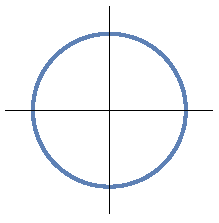
\includegraphics[width=\linewidth]{figures/unit-circle-vector.pdf}
\end{wrapfigure}
多项式及其解是我们学习数学时最早接触的一些对象. 例如, 你或许还记得第一次得知, 在 $\mathbb{R}^{2}$ 中, 二元多项式方程
\[
  x^{2}+y^{2}-1=0
\]
的解构成单位圆. 不过, 如果我们的目标是研究单位圆, 还可以选用许多其他多项式来描述它. 例如, 下列任一方程的解集也都是单位圆:
\[
  2x^{2}+2y^{2}-2=0
  \quad\text{或}\quad
  (x^{2}+y^{2}-1)^{2}=0.
\]
这就自然引出一个问题: 有没有一个描述单位圆的\textbf{最佳}多项式?
代数几何给出的答案, 在某种意义上是最平等的: 所有描述单位圆的多项式都同等重要, 我们应当把它们作为一个\textbf{集合}来研究.
那么, 研究一个多项式\textbf{集合}是什么意思呢?

我们很快就会看到, 描述单位圆的多项式所成的集合远不止是一个集合; 它具有重要的代数结构, 反映了圆的几何性质.
为了能描述这个例子及其他情形中的代数结构, 我们必须先为多项式集合及其代数结构确立准确的记号和术语.
我们从单项式的概念入手, 正式开始讨论多项式.

\begin{Definition}{单项式}\label{def:monomial}
  变量 $x_{1},\ldots,x_{n}$ 的\textbf{单项式}是形如
  \[
    x^{\alpha}=x_{1}^{\alpha_{1}}\cdots x_{n}^{\alpha_{n}},
  \]
  的表达式, 其中 $\alpha=(\alpha_{1},\ldots,\alpha_{n})\in\mathbb{N}^{n}$ 是\textbf{指数向量}.
  两个单项式相等, 当且仅当它们的指数向量相同.
\end{Definition}

\begin{BookFlowNote}{%
  变量只有几个时, 通常用不同的字母表示它们, 例如 \mbox{$x$, $y$ 和 $z$}.
}
变量 $x_{1},\ldots,x_{n}$ 应看作形式符号, 它们的作用只是充当 $\alpha_{1},\ldots,\alpha_{n}$ 的占位符.
一个关于 $x_{1},\ldots,x_{n}$ 的单项式所包含的信息, 与一个指数向量 $(\alpha_{1},\ldots,\alpha_{n})$ 所包含的信息是等价的; 不过, 把每个 $\alpha_{i}$ 写成 $x_{i}$ 的指数, 在下面定义单项式的乘法时会很有用.
指数为 $0$ 的变量通常省略不写. 例如,
\[
  x^{2}y^{3}z^{0}=x^{2}y^{3}
  \quad\text{且}\quad
  x^{0}y^{0}z^{0}=1.
\]
\end{BookFlowNote}
与 $f(x,y)=x^{2}+y^{2}-1$ 一样, 多项式由单项式的线性组合构成.
在最一般的情形下, 这些线性组合的系数属于任意环 $R$, 如下一个定义所示.


\begin{Definition}{环 \textmd{$R$} 上的多项式}\label{def:polynomial-over-ring}
  在环 $R$ 上, 关于变量 $x_{1},\ldots,x_{n}$ 的\textbf{多项式}是形如
  \[
    f=f(x_{1},\ldots,x_{n})=\sum_{\alpha\in\mathbb{N}^{n}}a_{\alpha}x^{\alpha},
  \]
  的表达式, 其中对每个 $\alpha\in\mathbb{N}^{n}$, 都有 $a_{\alpha}\in R$, 且除有限个 $\alpha$ 外, 均有 $a_{\alpha}=0$. 两个多项式
  \[
    f=\sum_{\alpha}a_{\alpha}x^{\alpha}
    \quad\text{和}\quad
    g=\sum_{\alpha}b_{\alpha}x^{\alpha}
  \]
  相等, 当且仅当对所有 $\alpha\in\mathbb{N}^{n}$, 都有 $a_{\alpha}=b_{\alpha}$.
\end{Definition}

\begin{Example}{多项式}\label{ex:polynomials-over-integers}
  \ExampleSideNote{下面是整数环 $\mathbb{Z}$ 上关于变量 $x$ 和 $y$ 的两个多项式:}%
    {多项式通常写成有限和, 省略所有系数为零的项.}
  \[
    f=xy^{2}+3xy+2
    \quad\text{和}\quad
    g=-xy+4.
  \]
  也可以把多项式 $f$ 和 $g$ 看作系数属于 $\mathbb{Q}$, $\mathbb{R}$, $\mathbb{C}$ 或任意其他包含 $\mathbb{Z}$ 的环的多项式.
  注意, 我们可以用熟悉的方式对 $f$ 和 $g$ 作加法和乘法, 从而得到新的多项式:
  \[
    \begin{gathered}
      f+g=xy^{2}+2xy+6,\\
      fg=-x^{2}y^{3}-3x^{2}y^{2}+4xy^{2}+10xy+8.
    \end{gathered}
  \]
\end{Example}

请读者在 Exercise~\ref{ex:polynomial-ring-laws} 中验证: 下一个定义中严格给出的加法和乘法, 使多项式的集合具有环结构.

\begin{Definition}{多项式环}\label{def:polynomial-ring}
  \textbf{多项式环} $R[x_{1},\ldots,x_{n}]$ 是环 $R$ 上关于变量 $x_{1},\ldots,x_{n}$ 的全体多项式的集合. 多项式加法和乘法定义如下:
  \[
    \left(\sum_{\alpha}a_{\alpha}x^{\alpha}\right)
    +\left(\sum_{\alpha}b_{\alpha}x^{\alpha}\right)
    =\sum_{\alpha}(a_{\alpha}+b_{\alpha})x^{\alpha}
  \]
  以及
  \[
    \left(\sum_{\alpha}a_{\alpha}x^{\alpha}\right)
    \left(\sum_{\alpha}b_{\alpha}x^{\alpha}\right)
    =\sum_{\alpha}\left(\sum_{\alpha_{1}+\alpha_{2}=\alpha}
      a_{\alpha_{1}}b_{\alpha_{2}}\right)x^{\alpha}.
  \]
\end{Definition}

加法单位元 $0\in R[x_{1},\ldots,x_{n}]$ 是对所有 $\alpha$ 均有 $a_{\alpha}=0$ 的多项式, 乘法单位元 $1\in R[x_{1},\ldots,x_{n}]$ 是满足下式的多项式:
\[
  a_{\alpha}=
  \begin{cases}
    1 & \text{若 }(\alpha_{1},\ldots,\alpha_{n})=(0,\ldots,0),\\
    0 & \text{若 }(\alpha_{1},\ldots,\alpha_{n})\ne(0,\ldots,0).
  \end{cases}
\]


研究多项式环时, 利用它的递归性质往往很有用, 因为这样便可对变量的个数使用归纳法. 下一个结果相当显然; 但由于经常要用到它, 我们仍仔细陈述如下.

\begin{Proposition}{多项式环的递归性质}\label{prop:polynomial-ring-recursion}
  有一个典范的环同构
  \[
    R[x_{1},\ldots,x_{n}]=R[x_{1},\ldots,x_{n-1}][x_{n}],
  \]
  其中右侧是系数属于环 $R[x_{1},\ldots,x_{n-1}]$ 的单变量 $x_{n}$ 多项式所成的环.
\end{Proposition}

下面的例子说明 Proposition~\ref{prop:polynomial-ring-recursion} 的主要思想.

\begin{Example}{{\textmd{$\mathbb{Z}[x,y]$} 与 \textmd{$\mathbb{Z}[x][y]$}}}\label{ex:iterated-polynomial-ring}
  考虑多项式
  \[
    f=x^{3}y^{2}+xy^{2}-2xy-x+1\in\mathbb{Z}[x,y].
  \]
  把 $y$ 的指数相同的所有项归在一起, 就可将 $f$ 看作 $\mathbb{Z}[x][y]$ 的元素. 这样写得
  \[
    f=(x^{3}+x)y^{2}+(-2x)y+(-x+1)\in\mathbb{Z}[x][y].
  \]
  作为 $y$ 的多项式, $f$ 的系数是 $x^{3}+x$, $-2x$ 和 $-x+1$, 它们都是 $\mathbb{Z}[x]$ 的元素.
\end{Example}

\begin{BookFlowNote}{%
  两个环同构时, 往往有许多可能的同构. \textquotedbl{}典范\textquotedbl{} 一词表示, 在所有可能的同构中有一个自然的选择.
  记号 $\cong$ 用来表示同构, 而 $=$ 用来表示典范同构.
}
\begin{Proof}\unskip\textbf{ of Proposition~\ref{prop:polynomial-ring-recursion}}\par\noindent
  为证明该命题, 我们来描述这个典范的环同构. 如 Example~\ref{ex:iterated-polynomial-ring} 所示, 它只是把 $R[x_{1},\ldots,x_{n}]$ 中某一个多项式内 $x_{n}$ 的指数相同的项归在一起.
  为了更精确地说明这一点, 考虑下列函数:
  \[
    \begin{aligned}
      \phi:R[x_{1},\ldots,x_{n}]&\to R[x_{1},\ldots,x_{n-1}][x_{n}]\\
      \sum_{\alpha\in\mathbb{N}^{n}}a_{\alpha}x_{1}^{\alpha_{1}}\cdots x_{n}^{\alpha_{n}}
      &\mapsto
      \sum_{d\ge0}\left(\sum_{\substack{\alpha\in\mathbb{N}^{n}\\\alpha_{n}=d}}
        a_{\alpha}x_{1}^{\alpha_{1}}\cdots x_{n-1}^{\alpha_{n-1}}\right)x_{n}^{d}.
    \end{aligned}
  \]
  验证 $\phi$ 是环同构, 见 Exercise~\ref{ex:recursive-ring-isomorphism}.
\end{Proof}
\end{BookFlowNote}

下面关于整环上的多项式环的结果, 是 Proposition~\ref{prop:polynomial-ring-recursion} 的第一个应用.


\begin{Proposition}{整环上的多项式}\label{prop:polynomials-over-domain}
  若 $R$ 是整环, 则 $R[x_{1},\ldots,x_{n}]$ 是整环.
\end{Proposition}

\begin{Proof}
  我们对变量的个数作归纳.

  \textbf{(归纳起点)} 设 $f,g\in R[x_{1}]$ 非零. 我们必须证明 $fg\ne0$. 写成
  \[
    f=a_{d}x_{1}^{d}+a_{d-1}x_{1}^{d-1}+\cdots+a_{0}
    \quad\text{且}\quad
    g=b_{e}x_{1}^{e}+b_{e-1}x_{1}^{e-1}+\cdots+b_{0},
  \]
  其中 $a_{d}\ne0$ 且 $b_{e}\ne0$. 根据 $R[x_{1}]$ 中乘法的定义,
  \[
    fg=(a_{d}b_{e})x_{1}^{d+e}
    +(a_{d}b_{e-1}+a_{d-1}b_{e})x_{1}^{d+e-1}+\cdots+a_{0}b_{0}.
  \]
  由于 $R$ 是整环, $a_{d}b_{e}\ne0$. 因为 $fg$ 至少有一个非零系数, 所以 $fg\ne0$.

  \textbf{(归纳步骤)} 假设 $S=R[x_{1},\ldots,x_{n-1}]$ 是整环; 我们必须证明 $R[x_{1},\ldots,x_{n}]$ 是整环. 由 Proposition~\ref{prop:polynomial-ring-recursion},
  \[
    R[x_{1},\ldots,x_{n}]=S[x_{n}].
  \]
  由于 $S$ 是整环, 归纳起点中的论证立即表明 $S[x_{n}]$, 从而 $R[x_{1},\ldots,x_{n}]$, 是整环.
\end{Proof}

Proposition~\ref{prop:polynomials-over-domain} 的证明中出现的数 $d$ 和 $e$ 是多项式 $f$ 和 $g$ 的重要属性, 称为它们的\textbf{次数}. 下一个定义把次数的概念推广到具有任意个变量的多项式.

\begin{Definition}{单项式和多项式的次数}\label{def:polynomial-degree}
  单项式 $x^{\alpha}=x_{1}^{\alpha_{1}}\cdots x_{n}^{\alpha_{n}}$ 的\textbf{次数}为
  \[
    \deg(x^{\alpha})=\alpha_{1}+\cdots+\alpha_{n}\in\mathbb{N}.
  \]
  非零多项式 $f=\sum a_{\alpha}x^{\alpha}\in R[x_{1},\ldots,x_{n}]$ 的\textbf{次数}为
  \[
    \deg(f)=\max\{\deg(x^{\alpha})\mid a_{\alpha}\ne0\}.
  \]
\end{Definition}

\begin{Example}{次数}\label{ex:monomial-and-polynomial-degrees}
  单项式 $x^{2}yz$, $z^{4}$, $x$ 和 $1$ 的次数分别为 $4$, $4$, $1$ 和 $0$, 并且
  \[
    \deg(x^{2}yz+z^{4}+x+1)=4.
  \]
\end{Example}

读者可能已经注意到, 我们没有给零多项式指定次数, 这是有意为之. 次数最有用的性质之一是下一个结果所述的\textbf{可加性}; 若选取任意 $\deg(0)\in\mathbb{N}$, 这个性质都不成立.



\begin{Proposition}{次数的可加性}\label{prop:degree-additivity}
  若 $R$ 是整环, 且 $f,g\in R[x_{1},\ldots,x_{n}]$ 非零, 则
  \[
    \deg(fg)=\deg(f)+\deg(g).
  \]
\end{Proposition}

\begin{Proof}
  设 $f,g\in R[x_{1},\ldots,x_{n}]$ 是次数分别为 $d$ 和 $e$ 的非零多项式. 写成
  \[
    f=f_{d}+f_{d-1}+\cdots+f_{0}
    \quad\text{和}\quad
    g=g_{e}+g_{e-1}+\cdots+g_{0},
  \]
  其中 $f_{i}$ 由 $f$ 中次数为 $i$ 的所有项组成, $g_{j}$ 类似. 由假设, $f_{d}\ne0$ 且 $g_{e}\ne0$.
  稍加思考便可看出, 单项式的次数具有可加性. 因此, $fg$ 中可能以非零系数出现的最高次单项式的次数为 $d+e$, 且来自乘积 $f_{d}g_{e}$.
  由于 $R[x_{1},\ldots,x_{n}]$ 是整环, 可知 $f_{d}g_{e}\ne0$, 从而得出 $\deg(fg)=d+e=\deg(f)+\deg(g)$.
\end{Proof}

\BookExerciseHeading
\begin{BookExercises}
  \item\label{ex:polynomial-ring-laws} 回顾环 (交换且含幺) 的定义, 并证明: 对任意环 $R$, 多项式的加法与乘法使 $R[x_{1},\ldots,x_{n}]$ 具有环 (交换且含幺) 的结构.
  \item\label{ex:regroup-three-variable-polynomial} 对多项式
    \[
      f=xyz^{2}+xyz+z^{3}+x^{2}z^{2}+yz^{2}+z+x+1\in R[x,y,z]
    \]
    的各项分组, 将其分别看作 $R[x,y][z]$, $R[x][y,z]$ 和 $R[y,z][x]$ 的元素.
  \item\label{ex:recursive-ring-isomorphism} 证明 Proposition~\ref{prop:polynomial-ring-recursion} 的证明中定义的函数
    \[
      \phi:R[x_{1},\ldots,x_{n}]\to R[x_{1},\ldots,x_{n-1}][x_{n}]
    \]
    是环同构.
  \item\label{ex:constant-polynomials-subring} 若只要 $\alpha\ne(0,\ldots,0)$ 就有 $a_{\alpha}=0$, 则称多项式 $f=\sum_{\alpha}a_{\alpha}x^{\alpha}\in R[x_{1},\ldots,x_{n}]$ 为常数多项式. 证明常数多项式的集合构成 $R[x_{1},\ldots,x_{n}]$ 中与 $R$ 同构的一个子环.
  \item\label{ex:evaluation-homomorphism} 设 $a=(a_{1},\ldots,a_{n})\in R^{n}$. 证明存在唯一的环同态
    \[
      \phi_{a}:R[x_{1},\ldots,x_{n}]\to R
    \]
    使得对所有 $r\in R$ 有 $\phi_{a}(r)=r$, 对所有 $i$ 有 $\phi_{a}(x_{i})=a_{i}$. (这个同态称为在 $a$ 处的求值, $\phi_{a}(f)$ 常写作 $f(a_{1},\ldots,a_{n})$.)
  \item\label{ex:failure-without-integral-domain} 说明若不假设 $R$ 是整环, Propositions~\ref{prop:polynomials-over-domain} 和 \ref{prop:degree-additivity} 不成立.
  \item\label{ex:degree-zero-polynomial} 说明无论怎样选取 $\deg(0)\in\mathbb{N}$, Proposition~\ref{prop:degree-additivity} 都不能推广到这一情形. (有些数学家采用约定 $\deg(0)=-\infty$.)
  \item\label{ex:degree-of-sum} 证明 $\deg(f+g)\leq\max\{\deg(f),\deg(g)\}$.
\end{BookExercises}


\section{不可约多项式}\label{sec:irreducible-polynomials}

代数几何主要关注系数取自域 $K$ 的多项式环 $K[x_{1},\ldots,x_{n}]$. (本节乃至全书始终用 $K$ 表示一个域.) 为了研究这些多项式环, 了解其中哪些元素是\textquotedbl{}原子\textquotedbl{}以及每个多项式如何分解成这类元素, 是很有用的. 为了引出这些概念, 不妨先考虑更熟悉的环 $\mathbb{Z}$, 其中的原子元素是素数.

回顾一下, 整数 $p\in\mathbb{Z}_{\geq2}$ 是\textbf{素数}, 如果对所有 $m,n\in\mathbb{Z}$ 都有
\begin{equation}\label{eq:prime-integer-factor-test}
  p=mn\implies m=\pm1\quad\text{或}\quad n=\pm1.
\end{equation}
换言之, 素数是不能作非平凡分解的整数. 数论 (乃至整个数学) 的核心结果之一是素因数分解的存在性和唯一性: 每个整数 $n\in\mathbb{Z}_{\geq2}$ 都可以写成素数的乘积, 若不计因子的排列顺序, 这种写法是唯一的.

我们希望在更一般的情形下研究这些概念, 特别是在多项式环中. 为此, 先从环论中\textquotedbl{}原子\textquotedbl{}的定义开始, 其中包括可逆元的概念, 它推广了 \eqref{eq:prime-integer-factor-test} 中出现的 $\pm1\in\mathbb{Z}$.

\begin{Definition}{可逆元与(不)可约元}\label{def:units-irreducible-elements}
  若元素 $u\in R$ 有乘法逆元, 就称它为\textbf{可逆元}. $R$ 中可逆元的集合记为 $R^{*}\subseteq R$. 称元素 $p\in R$ 为\textbf{不可约元}, 如果它既非零也不是可逆元, 并且
  \[
    p=ab\implies a\in R^{*}\quad\text{或}\quad b\in R^{*}.
  \]

  若一个元素既非零, 也不是可逆元或不可约元, 则它是\textbf{可约元}.
\end{Definition}

\BookPairedNote{换言之, 一个非零元素如果不能分解成两个非可逆元的乘积, 就是不可约元. 对域 $K$ 上的多项式环 $K[x_{1},\ldots,x_{n}]$ 而言, 可逆元是非零常数多项式 (Exercise~\ref{ex:units-polynomial-ring-over-field}):}%
  {必须区分可逆元与非可逆元, 因为若允许可逆元, 则每个元素都能分解:
   \[
     a=u(u^{-1}a).
   \]}
\[
  K[x_{1},\ldots,x_{n}]^{*}=K^{*}=K\setminus\{0\}.
\]
因此, 多项式 $f\in K[x_{1},\ldots,x_{n}]$ 不可约, 当且仅当
\begin{enumerate}[label=(\roman*)]
  \item $f$ 不是常数多项式, 且
  \item $f$ 不能写成两个非常数多项式的乘积.
\end{enumerate}

\begin{Example}{{\textmd{$K[x_{1},\ldots,x_{n}]$} 中的一次多项式不可约}}
  \leavevmode\label{ex:linear-polynomials-irreducible}\strut\par\nopagebreak[4]\noindent
  若 $\deg(f)=1$, 就称多项式 $f\in K[x_{1},\ldots,x_{n}]$ 为\textbf{一次多项式}. 若 $f$ 是一次多项式且 $f=gh$, 则由次数的可加性,
  \[
    1=\deg(f)=\deg(g)+\deg(h).
  \]
  因此, $\deg(g)=0$ 或 $\deg(h)=0$, 这说明 $g$ 或 $h$ 是常数多项式.
\end{Example}

\begin{Example}{{\textmd{$y-x^{2}$} 在 \textmd{$K[x,y]$} 中不可约}}\label{ex:parabola-polynomial-irreducible}
  设
  \[
    y-x^{2}=gh
  \]
  对某些 $g,h\in K[x,y]$ 成立. 作为环 $K[x][y]$ 的元素, 多项式 $y-x^{2}$ 的次数为 $1$, 因此 (作为关于 $y$ 的多项式) $g$ 与 $h$ 中一个的次数必为 $1$, 另一个的次数必为 $0$. 不失一般性, 可写成
  \[
    g=ay+b\quad\text{且}\quad h=c
  \]
  其中 $a,b,c\in K[x]$. 由此得到 $y-x^{2}=acy+bc$. 比较 $y$ 的系数, 可知 $ac=1$, 从而 $h=c\in K^{*}$. 因此, $y-x^{2}$ 不可约.
\end{Example}

\begin{Example}{{\textmd{$x^{2}+1\in\mathbb{C}[x]$} 与 \textmd{$x^{2}+1\in\mathbb{R}[x]$}}}\label{ex:quadratic-over-complex-and-real}
  在 $\mathbb{C}[x]$ 中, 有分解
  \[
    x^{2}+1=(x-\mathrm{i})(x+\mathrm{i}),
  \]
  这表明 $x^{2}+1$ 在 $\mathbb{C}[x]$ 中可约. 另一方面, 在 $\mathbb{R}[x]$ 中不可能将 $x^{2}+1$ 分解成两个一次因子 (Exercise~\ref{ex:quadratic-no-real-linear-factors}), 所以 $x^{2}+1$ 在 $\mathbb{R}[x]$ 中不可约. 这个例子说明, 多项式环的性质很大程度上取决于系数环的选取.
\end{Example}

素因数分解是整数环的一项基本性质, 将它推广到整环的情形是有用的. 下面的定义抓住了 $\mathbb{Z}$ 中唯一素因数分解的要点.

\begin{Definition}{唯一分解整环}\label{def:unique-factorization-domain}
  若满足下述条件, 整环 $R$ 称为\textbf{分解整环} (FD):
  \begin{enumerate}[label=(\roman*)]
    \item 对每个非零且不可逆的 $a\in R$, 都存在不可约元 $p_{1},\ldots,p_{\ell}\in R$, 使得 $a=p_{1}\cdots p_{\ell}$.
  \end{enumerate}
  若此外还满足下述条件, 就称它为\textbf{唯一分解整环} (UFD):
  \begin{enumerate}[label=(\roman*),start=2]
    \item 只要不可约元 $p_{i}$ 和 $q_{j}$ 满足 $p_{1}\cdots p_{\ell}=q_{1}\cdots q_{m}$, 就有 $\ell=m$, 且在必要时重新排列后, 存在可逆元 $u_{i}$, 使对所有 $i$ 都有 $p_{i}=u_{i}q_{i}$.
  \end{enumerate}
\end{Definition}

整数环中的唯一素因数分解说明 $\mathbb{Z}$ 是 UFD. $K[x_{1},\ldots,x_{n}]$ 的一个基本性质是它也是 UFD, 这一点我们将在本章陆续看到.

\BookPairedNote{要证明 $K[x_{1},\ldots,x_{n}]$ 是 UFD, 就要证明不可约分解存在且唯一. 本节只证明不可约分解的存在性.}%
  {一个不是 FD 的整环和一个不是 UFD 的 FD, 分别见 Exercises~\ref{ex:domain-without-factorization} 和 \ref{ex:factorization-domain-not-unique}.}

\begin{Proposition}{{\textmd{$K[x_{1},\ldots,x_{n}]$} 是 FD}}\label{prop:polynomial-factorization-exists}
  如果 $f\in K[x_{1},\ldots,x_{n}]$ 是非常数多项式, 则存在不可约多项式 $p_{1},\ldots,p_{\ell}\in K[x_{1},\ldots,x_{n}]$, 使得 $f=p_{1}\cdots p_{\ell}$.
\end{Proposition}

\begin{Proof}
  对 $f$ 的次数作归纳.

  \textbf{(归纳起点)} 如果 $\deg(f)=1$, 则由 Example~\ref{ex:linear-polynomials-irreducible}, $f$ 不可约. 特别地, $f$ 有一个不可约分解 (其中 $\ell=1$).

  \textbf{(归纳步骤)} 假设每个次数小于 $d$ 的多项式都能分解成不可约多项式的乘积, 并设 $f\in K[x_{1},\ldots,x_{n}]$ 的次数为 $d$. 若 $f$ 不可约, 则它有一个 $\ell=1$ 的不可约分解. 若 $f$ 不是不可约多项式, 则 $f=gh$, 其中 $\deg(g)<d$ 且 $\deg(h)<d$. 由归纳假设, 有不可约分解
  \[
    g=p_{1}\cdots p_{\ell}\quad\text{和}\quad h=q_{1}\cdots q_{k}.
  \]
  因此, $f$ 有一个不可约分解
  \[
    f=p_{1}\cdots p_{\ell}\cdot q_{1}\cdots q_{k}.
  \]
\end{Proof}

\begin{Example}{一个不可约分解}\label{ex:irreducible-factorization-complex-quadratic}
  由 Examples~\ref{ex:linear-polynomials-irreducible} 和 \ref{ex:quadratic-over-complex-and-real} 可知,
  \[
    x^{2}+1=(x-\mathrm{i})(x+\mathrm{i})
  \]
  是 $x^{2}+1\in\mathbb{C}[x]$ 的一个不可约分解.
\end{Example}

为了寻找证明不可约分解唯一性的思路, 我们回到熟悉的 $\mathbb{Z}$. 证明整数的素因数分解唯一的关键是 Euclid's Lemma: $p\in\mathbb{Z}_{\geq2}$ 是素数, 当且仅当对所有 $m,n\in\mathbb{Z}$ 都有
\BookPairedNote{%
  \[
    p\mid mn\implies p\mid m\quad\text{或}\quad p\mid n.
  \]
  素数的第二种刻画可以自然地推广到环.}%
  {我们用标准记号 $a\mid b$ 表示\textquotedbl{}$a$ 整除 $b$\textquotedbl{}, 即对某个 $c$, 有 $b=ca$.}

\begin{Definition}{素元}\label{def:prime-element}
  称元素 $p\in R$ 为\textbf{素元}, 如果它既不是零也不是可逆元, 且对所有 $a,b\in R$ 都有
  \[
    p\mid ab\implies p\mid a\quad\text{或}\quad p\mid b.
  \]
\end{Definition}

如下面将要看到的, 不可约分解是否唯一的问题, 可以归结为证明 Euclid's Lemma 在环论中的对应结论. 更确切地说, 给定整环 $R$, Euclid's Lemma 可转化为 $R$ 中的素元与不可约元一致的陈述. 下面的结果验证其中一个方向: 在整环中, 所有素元都是不可约元.

\begin{Proposition}{素元必不可约}\label{prop:prime-implies-irreducible}
  在整环中, 每个素元都是不可约元.
\end{Proposition}

\begin{Proof}
  设 $R$ 是整环, $p\in R$ 是素元. 为了证明 $p$ 不可约, 假设
  \begin{equation}\label{eq:prime-element-factorization}
    p=ab\quad\text{对某些}\quad a,b\in R;
  \end{equation}
  我们必须证明 $a\in R^{*}$ 或 $b\in R^{*}$. 注意, 由 \eqref{eq:prime-element-factorization} 特别可得 $p\mid ab$. 由于 $p$ 是素元, 有 $p\mid a$ 或 $p\mid b$. 不失一般性, 假设 $p\mid a$, 写成 $a=pc$, 其中 $c\in R$. 把这个表达式代入 \eqref{eq:prime-element-factorization}, 得
  \[
    p=pcb.
  \]
  由于 $R$ 是整环且 $p\ne0$, 可以从等式两边约去 $p$, 得到 $1=cb$, 所以 $b\in R^{*}$.
\end{Proof}

\BookPairedNote{Proposition~\ref{prop:prime-implies-irreducible} 的逆命题一般不成立. 实际上, 在某种意义上, 逆命题等价于分解的唯一性, 这就是下一个结果的内容.}%
  {Proposition~\ref{prop:prime-implies-irreducible} 的逆命题不成立的一个例子, 见后面的 Exercise~\ref{ex:factorization-domain-not-unique}.}

\begin{Proposition}{FD 与 UFD}\label{prop:ufd-iff-irreducibles-prime}
  设 $R$ 是一个分解整环. 则 $R$ 是唯一分解整环, 当且仅当 $R$ 的每个不可约元都是素元.
\end{Proposition}

\begin{Proof}
  我们证明两个方向.

  ($\implies$) 假设 $R$ 是 UFD, 设 $p\in R$ 不可约. 为了证明 $p$ 是素元, 假设对某些 $a,b\in R$ 有 $p\mid ab$, 并选取 $c\in R$, 使得 $ab=pc$. 由于 $R$ 是 FD, 每个元素都可以作不可约分解:
  \[
    a=p_{1}\cdots p_{k},\quad b=q_{1}\cdots q_{\ell},\quad\text{且}\quad c=r_{1}\cdots r_{m}.
  \]
  因此, 有两个不可约分解:
  \[
    p_{1}\cdots p_{k}\cdot q_{1}\cdots q_{\ell}=p\cdot r_{1}\cdots r_{m}.
  \]
  由于 $R$ 是 UFD, 存在可逆元 $u$, 使得对某个 $i$ 或 $j$ 有 $p=up_{i}$ 或 $p=uq_{j}$. 因而 $p\mid a$ 或 $p\mid b$, 所以 $p$ 是素元.

  ($\impliedby$) 假设 $R$ 的每个不可约元都是素元, 设
  \begin{equation}\label{eq:two-irreducible-factorizations}
    p_{1}\cdots p_{\ell}=q_{1}\cdots q_{m}
  \end{equation}
  是两个由不可约元 (因而是素元) 给出的分解. 不失一般性, 假设 $\ell\leq m$. 由于 $p_{1}$ 是素元且 $p_{1}\mid q_{1}\cdots q_{m}$, 由 Exercise~\ref{ex:prime-divides-one-of-factors} 可知, 对某个 $j$ 有 $p_{1}\mid q_{j}$. 必要时重新排列, 可设 $j=1$, 并写成 $q_{1}=u_{1}p_{1}$, 其中 $u_{1}\in R$. 因为 $q_{1}$ 不可约, $u_{1}$ 或 $p_{1}$ 必为可逆元. 但 $p_{1}$ 不可约, 不可能是可逆元. 因此, $u_{1}$ 是可逆元. 在 \eqref{eq:two-irreducible-factorizations} 的两边约去 $p_{1}$, 得
  \[
    p_{2}\cdots p_{\ell}=u_{1}q_{2}\cdots q_{m}.
  \]
  由于 $p_{2}\nmid u_{1}$ (否则 $p_{2}$ 本身就是可逆元), 可以重复上述论证, 得知必要时重新排列后, 存在可逆元 $u_{2}\in R$, 使得 $q_{2}=u_{2}p_{2}$, 且
  \[
    p_{3}\cdots p_{\ell}=u_{1}u_{2}q_{3}\cdots q_{m}.
  \]
  这样继续进行 $\ell$ 步, 可知有可逆元 $u_{1},\ldots,u_{\ell}$, 使得 $q_{i}=u_{i}p_{i}$, 而且
  \[
    1=u_{1}\cdots u_{\ell}q_{\ell+1}\cdots q_{m}.
  \]
  由于每个 $q_{j}$ 都不可约, 因而不是可逆元, 于是 $\ell=m$. 这就完成了 $R$ 是 UFD 的证明.
\end{Proof}

既然已知 $K[x_{1},\ldots,x_{n}]$ 是 FD, Proposition~\ref{prop:ufd-iff-irreducibles-prime} 就给出了证明 $K[x_{1},\ldots,x_{n}]$ 是 UFD 的办法: 只须证明每个不可约多项式都是素元. 为了做到这一点, 我们需要更扎实的代数基础来处理这些概念. 为此, 我们先讨论理想与商 (Section~{\ref{sec:ideals-quotients}}), 素理想与极大理想 (Section~{\ref{sec:prime-maximal-ideals}}), 以及一元多项式这一特殊情形 (Section~{\ref{sec:single-variable-polynomials}}). 然后在 Section~{\ref{sec:unique-factorization-polynomial-rings}} 中回到多项式的唯一分解.

\BookExerciseHeading
\begin{BookExercises}
  \item\label{ex:units-form-group} 证明可逆元的集合 $R^{*}\subseteq R$ 在乘法下构成一个群.
  \item\label{ex:units-polynomial-ring-over-field} 证明 $K[x_{1},\ldots,x_{n}]^{*}=K^{*}=K\setminus\{0\}$.
  \item\label{ex:quadratic-no-real-linear-factors} 利用对任何实数 $a\in\mathbb{R}$ 都有 $a^{2}+1\ne0$ 这一事实, 证明 $x^{2}+1$ 在 $\mathbb{R}[x]$ 中不能分解成一次因子的乘积.
  \item\label{ex:quadratic-cubic-irreducible-root-test} 设 $f\in K[x]$ 是次数为 $2$ 或 $3$ 的多项式. 证明: $f$ 不可约, 当且仅当不存在元素 $a\in K$ 使得 $f(a)=0$.
  \item\label{ex:quartic-no-real-zeros-reducible} 给出一个 $\mathbb{R}[x]$ 中可约且无零点的显式例子, 说明上一题对四次多项式不成立.
  \item\label{ex:circle-polynomial-irreducible-over-complex} 用次数论证证明 $x^{2}+y^{2}-1$ 在 $\mathbb{C}[x,y]$ 中不可约.
  \item\label{ex:prime-divides-one-of-factors} 假设 $p\in R$ 是素元. 若 $p\mid a_{1}\cdots a_{n}$, 证明对某个 $i$ 有 $p\mid a_{i}$.
  \item\label{ex:units-zz-polynomial-and-reducible-linear}
    \begin{enumerate}[label=(\alph*)]
      \item 描述 $\mathbb{Z}[x]$ 中的可逆元.
      \item 给出一个 $\mathbb{Z}[x]$ 中可约的一次多项式的例子.
    \end{enumerate}
  \item\label{ex:field-is-ufd} 说明为什么每个域都是 UFD.
  \item\label{ex:domain-without-factorization} 考虑环 $R=\{f\in\mathbb{Q}[x]\mid f(0)\in\mathbb{Z}\}\subseteq\mathbb{Q}[x]$.
    \begin{enumerate}[label=(\alph*)]
      \item 证明 $R$ 是整环.
      \item 证明元素 $x\in R$ 既不是可逆元也不是不可约元.
      \item 证明 $x\in R$ 不能分解成不可约元的乘积, 因此 $R$ 不是 FD.
    \end{enumerate}
\end{BookExercises}


\section{理想与商}\label{sec:ideals-quotients}

对理想取商是环论的核心构造之一. 本节回顾取商构造, 以及关于商的最基本的结果: 第一同构定理. 理想和商环是环论入门课程的标准论题, 因而本节把证明留作习题. 不过, 我们会给出若干有启发性的例子, 说明在多项式环中怎样处理理想和商.

我们从理想的概念开始讨论商环.

\begin{Definition}{理想}\label{def:ideal}
  $R$ 的\textbf{理想}是满足以下两个性质的非空子集 $I\subseteq R$:
  \begin{enumerate}[label=(\roman*)]
    \item $a,b\in I\implies a-b\in I$, 且
    \item $a\in I$ 且 $r\in R\implies ra\in I$.
  \end{enumerate}
\end{Definition}

换言之, 环的一个非空子集是理想, 如果它 (i) 对减法封闭, 且 (ii) 对乘法有吸收性. 在许多情形下, 描述理想最简单的方法是指定一个生成集. 下面的定义明确了这种描述方法.

\begin{Definition}{理想的生成集}\label{def:ideal-generating-set}
  若 $A\subseteq R$ 是一个子集, 则 \textbf{由 $A$ 生成的理想}, 记作 $\langle A\rangle$, 是 $A$ 中元素的所有 $R$-线性组合所成的集合:
  \[
    \langle A\rangle=
    \left\{\left.\sum_{i=1}^{n}r_{i}a_{i}\ \right|\;
    n\in\mathbb{N},\ r_{1},\ldots,r_{n}\in R,\ a_{1},\ldots,a_{n}\in A\subseteq R\right\}.
  \]
  若 $A=\{a_{1},\ldots,a_{n}\}$ 是有限集, 则写成 $\langle A\rangle=\langle a_{1},\ldots,a_{n}\rangle$. 能由单个元素生成的理想称为\textbf{主理想}.
\end{Definition}

读者不妨验证, 集合 $\langle A\rangle$ 确实是一个理想. 此外, 它是 $R$ 中包含集合 $A$ 的最小理想 (Exercise~\ref{ex:ideal-generated-by-set}). 下面给出 $R[x_{1},\ldots,x_{n}]$ 中一个理想及其生成集的具体例子.

\begin{Example}{{\textmd{$R[x_{1},\ldots,x_{n}]$} 中一个理想的生成元}}\label{ex:vanishing-constant-ideal}
  设 $I\subseteq R[x_{1},\ldots,x_{n}]$ 是全体常数项为零的多项式所成的子集. 这些多项式所成的集合对减法封闭, 并且对乘法有吸收性, 因此 $I$ 是理想. 此外, 一个多项式属于 $I$, 当且仅当它的每一项都能提出至少一个变量作为因子. 由此可知 $I=\langle x_{1},\ldots,x_{n}\rangle$.
\end{Example}

根据定义, 主理想 $\langle a\rangle$ 由其生成元的所有倍数组成:
\[
  \langle a\rangle=\{ra\mid r\in R\}=\{b\in R\mid a\text{ 整除 }b\}.
\]
主理想特别便于处理, 但多项式环中的理想并不都是主理想; 例如, Example~\ref{ex:vanishing-constant-ideal} 中的理想就不是主理想 (Exercise~\ref{ex:variables-ideal-not-principal}).

给定理想 $I\subseteq R$, 如下定义 $R$ 上的一个关系:
\[
  r\sim s\iff r-s\in I.
\]
利用 Definition~\ref{def:ideal} 的条件 (i) 可以证明, $\sim$ 是一个等价关系 (Exercise~\ref{ex:coset-relation-equivalence}). 元素 $r\in R$ 在这一等价关系下的等价类称为\textbf{陪集}, 记为
\[
  [r]=r+I=\{s\in R\mid s\sim r\}\subseteq R.
\]
若上下文中理想 $I$ 已经明确, 我们通常优先采用记号 $[r]$; 在需要强调 $I$ 的作用时, 则用记号 $r+I$. 注意,
\[
  [r]=[s]\iff r-s\in I.
\]

\begin{Example}{陪集}\label{ex:cosets-of-variable-ideal}
  考虑主理想 $I=\langle x\rangle\subseteq R[x]$. 注意, $[x+2]=[x^{2}+2]$, 因为
  \[
    (x+2)-(x^{2}+2)=x-x^{2}\in\langle x\rangle.
  \]
  更一般地, $[f(x)]=[g(x)]$ 当且仅当 $f(0)=g(0)\in R$. 换言之, 全体陪集与环 $R$ 通过下面的对应构成自然双射:
  \[
    [f(x)]\longmapsto f(0)\in R.
  \]
\end{Example}

在上一个例子中, 我们看到全体陪集与系数环 $R$ 双射, 因而可以赋予它环结构. 下一个定义说明, 对任意理想, 怎样在陪集的集合上赋予环结构.

\begin{Definition}{商环}\label{def:quotient-ring}
  设 $I\subseteq R$ 是理想. \textbf{商环} $R/I$ 是陪集的集合
  \[
    R/I=\{[r]\mid r\in R\}.
  \]
  陪集的加法和乘法定义为
  \[
    [r]+[s]=[r+s]\quad\text{且}\quad[r][s]=[rs].
  \]
\end{Definition}

\BookPairedNote{$R/I$ 中的加法和乘法是否良定义, 并不是显然的. 特别是, 同一个陪集可以选择不同的元素来代表, 所以必须核实这两种运算都不依赖于陪集代表元的选取.}%
  {在商环 $R/I$ 中, 加法单位元为 $0=[0]$, 乘法单位元为 $1=[1]$. 因为 $[a]=0$ 当且仅当 $a\in I$, 所以可以把取商理解为\textquotedbl{}令 $I$ 中的元素等于零\textquotedbl{}.}
\noindent 这一点可由 Definition~\ref{def:ideal} 的条件 (i) 和 (ii) 得出; 我们把具体计算留给读者 (Exercise~\ref{ex:quotient-operations-well-defined}).

注意, 对任意理想 $I\subseteq R$, 存在一个环同态
\[
  \begin{aligned}
    \pi:R&\to R/I\\
    a&\mapsto[a].
  \end{aligned}
\]
这个同态称为\textbf{商同态}.

\begin{Example}{商环中的计算}\label{ex:quotient-parabola-computations}
  考虑主理想 $\langle y-x^{2}\rangle\subseteq R[x,y]$. 由商环中加法和乘法的定义可得
  \[
    [y]-[x]^{2}=[y-x^{2}]=0\in\frac{R[x,y]}{\langle y-x^{2}\rangle}.
  \]
  特别地, 这说明 $[y]=[x]^{2}$. 再往前一步, 例如可以得到
  \[
    [y]^{2}=[x]^{4}\quad\text{且}\quad[x]^{2}[y]^{3}=[x]^{8}.
  \]
  一般地, 对任意多项式 $f(x,y)\in R[x,y]$, 注意到
  \[
    [f(x,y)]=f([x],[y])=f([x],[x]^{2})=[f(x,x^{2})].
  \]
  换言之, 对理想 $\langle y-x^{2}\rangle$ 取商时, 可以把 $y-x^{2}$ 当作零元, 并把所有出现的 $y$ 都换成 $x^{2}$. 特别地, 商环的每个元素都可以仅用变量 $x$ 表示. 如下面的 Example~\ref{ex:quotient-parabola-isomorphism} 所示, 本例中的商环与 $R[x]$ 同构.
\end{Example}

取商构造最重要的应用, 是提供了一种把同态化为同构的工具. 下面这一基本结果的三点证明都留给读者 (Exercise~\ref{ex:prove-first-ring-isomorphism-theorem}).

\begin{Theorem}{环的第一同构定理}\label{thm:first-isomorphism-theorem-for-rings}
  若 $\phi:R\to S$ 是环同态, 则
  \begin{enumerate}[label=(\roman*)]
    \item $\operatorname{im}(\phi)=\{s\in S\mid s=\phi(r)\text{ 对某个 }r\in R\text{ 成立}\}$ 是 $S$ 的子环,
    \item $\ker(\phi)=\{r\in R\mid\phi(r)=0\}$ 是 $R$ 的理想, 且
    \item 函数
      \[
        \begin{aligned}
          [\phi]:\frac{R}{\ker(\phi)}&\to\operatorname{im}(\phi)\\
          [r]&\mapsto[\phi(r)]
        \end{aligned}
      \]
      是一个良定义的环同构.
  \end{enumerate}
\end{Theorem}

本节最后给出若干详细例子, 说明第一同构定理在多项式环中的应用. 更多例子见本节习题.

\begin{Example}{{\textmd{$\langle x_{1},\ldots,x_{n}\rangle\subseteq R[x_{1},\ldots,x_{n}]$}}}
  \leavevmode\label{ex:quotient-evaluation-origin}\strut\par\nopagebreak[4]\noindent
  考虑环同态
  \[
    \begin{aligned}
      \phi:R[x_{1},\ldots,x_{n}]&\to R\\
      f(x_{1},\ldots,x_{n})&\mapsto f(0,\ldots,0).
    \end{aligned}
  \]
  注意, $f(0,\ldots,0)$ 就是 $f$ 的常数项. 稍加思考便可看出, $\phi$ 是满射, 而 $\phi$ 的核由所有常数项为零的多项式组成. 因此, 由 Example~\ref{ex:vanishing-constant-ideal},
  \[
    \ker(\phi)=\langle x_{1},\ldots,x_{n}\rangle\subseteq R[x_{1},\ldots,x_{n}],
  \]
  再由第一同构定理, 可知 $[\phi]$ 给出一个同构:
  \[
    \frac{R[x_{1},\ldots,x_{n}]}{\langle x_{1},\ldots,x_{n}\rangle}\cong R.
  \]
  通过类似论证, 可以用多种方式推广本例. 例如, 见 Exercises~\ref{ex:quotient-set-last-variables-zero} 和 \ref{ex:quotient-evaluation-at-point}.
\end{Example}

\begin{Example}{{\textmd{$\langle y-x^{2}\rangle\subseteq R[x,y]$}}}\label{ex:quotient-parabola-isomorphism}
  本例验证
  \[
    \frac{R[x,y]}{\langle y-x^{2}\rangle}\cong R[x].
  \]
  根据 Example~\ref{ex:quotient-parabola-computations} 的计算, 这个结论是合乎情理的: 我们可以把所有出现的 $y$ 换成 $x^{2}$, 从而仅用 $x$ 来写每个陪集. 要借助第一同构定理把这一论证说得确切, 只须构造一个满同态 $\phi:R[x,y]\to R[x]$, 使它的核为 $\langle y-x^{2}\rangle$.

  定义
  \[
    \begin{aligned}
      \phi:R[x,y]&\to R[x]\\
      f(x,y)&\mapsto f(x,x^{2}),
    \end{aligned}
  \]
  读者可以验证, 这是一个满的环同态. 因此, 只需证明 $\langle y-x^{2}\rangle=\ker(\phi)$. 我们证明两个包含关系.

  ($\subseteq$) 设 $f(x,y)\in\langle y-x^{2}\rangle$. 这意味着存在 $g(x,y)\in R[x,y]$, 使得
  \[
    f(x,y)=(y-x^{2})g(x,y).
  \]
  对 $f(x,y)$ 应用 $\phi$, 可得
  \[
    \phi(f(x,y))=(x^{2}-x^{2})g(x,x^{2})=0,
  \]
  所以 $f(x,y)\in\ker(\phi)$.

  ($\supseteq$) 设 $f(x,y)\in\ker(\phi)$. 根据 Example~\ref{ex:quotient-parabola-computations} 的计算, 可知在商环 $R[x,y]/\langle y-x^{2}\rangle$ 中, $[f(x,y)]=[f(x,x^{2})]$, 因而
  \begin{equation}\label{eq:parabola-substitution-difference}
    f(x,y)-f(x,x^{2})\in\langle y-x^{2}\rangle.
  \end{equation}
  此外, 因为 $f(x,y)\in\ker(\phi)$, 所以
  \begin{equation}\label{eq:parabola-substitution-zero}
    0=\phi(f(x,y))=f(x,x^{2})\in R[x]\subseteq R[x,y].
  \end{equation}
  结合 \eqref{eq:parabola-substitution-zero} 与 \eqref{eq:parabola-substitution-difference}, 可得
  \[
    f(x,y)=f(x,y)-f(x,x^{2})\in\langle y-x^{2}\rangle.
  \]
  Exercise~\ref{ex:quotient-substitute-polynomial} 给出了这个结果的一个有用的推广.
\end{Example}

\BookExerciseHeading
\begin{BookExercises}
  \item\label{ex:ideal-containing-unit} 设 $I\subseteq R$ 是理想. 证明: $I=R$ 当且仅当 $I$ 包含一个可逆元.
  \item\label{ex:ideal-zero-and-addition} 证明理想包含 $0$, 并且对加法封闭.
  \item\label{ex:ideals-of-field} 证明域 $K$ 只有 $\{0\}$ 和 $K$ 这两个理想.
  \item\label{ex:ideal-generated-by-set} 设 $A\subseteq R$ 是子集. 证明以下结论.
    \begin{enumerate}[label=(\alph*)]
      \item 集合 $\langle A\rangle$ 是 $R$ 的理想.
      \item 若 $I\subseteq R$ 是包含 $A$ 的任意理想, 则 $\langle A\rangle\subseteq I$.
    \end{enumerate}
  \item\label{ex:variables-ideal-not-principal} 证明当 $n>1$ 时, $\langle x_{1},\ldots,x_{n}\rangle\subseteq K[x_{1},\ldots,x_{n}]$ 不是主理想.
  \item\label{ex:coset-relation-equivalence} 设 $I\subseteq R$ 是理想, 考虑 $R$ 上的关系
    \[
      r\sim s\iff r-s\in I.
    \]
    \begin{enumerate}[label=(\alph*)]
      \item 证明 $\sim$ 是自反的: 对所有 $r\in R$, 都有 $r\sim r$.
      \item 证明 $\sim$ 是对称的: $r\sim s$ 蕴涵 $s\sim r$.
      \item 证明 $\sim$ 是传递的: 若 $r\sim s$ 且 $s\sim t$, 则 $r\sim t$.
    \end{enumerate}
    因此, $\sim$ 是一个等价关系.
  \item\label{ex:coset-representative-sum} 给定理想 $I\subseteq R$, 证明 $[r]=\{r+a\mid a\in I\}$, 从而说明记号 $[r]=r+I$ 是合理的.
  \item\label{ex:quotient-operations-well-defined} 设 $I\subseteq R$ 是理想, 且 $r_{1},r_{2},s\in R$. 证明以下结论.
    \begin{enumerate}[label=(\alph*)]
      \item 若 $r_{1}\sim r_{2}$, 则 $r_{1}+s\sim r_{2}+s$.
      \item 若 $r_{1}\sim r_{2}$, 则 $r_{1}s\sim r_{2}s$.
    \end{enumerate}
    因此, 商环 $R/I$ 中的加法和乘法是良定义的.
  \item\label{ex:prove-first-ring-isomorphism-theorem} 论证环的第一同构定理.
  \item\label{ex:ideal-images-and-preimages} 设 $\phi:R\to S$ 是环同态.
    \begin{enumerate}[label=(\alph*)]
      \item 若 $I\subseteq S$ 是理想, 证明 $\phi^{-1}(I)\subseteq R$ 是理想.
      \item 若 $\phi$ 是满射且 $I\subseteq R$ 是理想, 证明 $\phi(I)\subseteq S$ 是理想.
      \item 举出一个非满的环同态 $\phi:R\to S$ 和一个理想 $I\subseteq R$, 使得 $\phi(I)$ 不是理想.
    \end{enumerate}
  \item\label{ex:quotient-set-last-variables-zero} 证明
    \[
      \frac{R[x_{1},\ldots,x_{n}]}{\langle x_{k+1},\ldots,x_{n}\rangle}\cong R[x_{1},\ldots,x_{k}].
    \]
  \item\label{ex:quotient-evaluation-at-point} 设 $a_{1},\ldots,a_{n}$ 是 $R$ 的元素. 证明
    \[
      \frac{R[x_{1},\ldots,x_{n}]}{\langle x_{1}-a_{1},\ldots,x_{n}-a_{n}\rangle}\cong R.
    \]
  \item\label{ex:quotient-substitute-polynomial} 设 $f_{1},\ldots,f_{k}\in R[x_{1},\ldots,x_{n}]$, 且 $g\in R[x_{1},\ldots,x_{n-1}]$. 考虑环同态
    \[
      \begin{aligned}
        \phi:R[x_{1},\ldots,x_{n}]&\to R[x_{1},\ldots,x_{n-1}]\\
        f(x_{1},\ldots,x_{n-1},x_{n})&\mapsto f(x_{1},\ldots,x_{n-1},g).
      \end{aligned}
    \]
    利用第一同构定理证明
    \[
      \frac{R[x_{1},\ldots,x_{n}]}{\langle f_{1},\ldots,f_{k},x_{n}-g\rangle}
      \cong\frac{R[x_{1},\ldots,x_{n-1}]}{\langle\phi(f_{1}),\ldots,\phi(f_{k})\rangle}.
    \]
    (注意, Examples~\ref{ex:quotient-evaluation-origin} 和 \ref{ex:quotient-parabola-isomorphism}, 以及 Exercises~\ref{ex:quotient-set-last-variables-zero} 和 \ref{ex:quotient-evaluation-at-point}, 都是这个结果的推论. 这一结果实质上说明, 对 $x_{n}-g$ 取商等价于把所有出现的 $x_{n}$ 换成 $g$.)
  \item\label{ex:unit-circle-quotient-normal-form} 证明商环
    \[
      \frac{R[x,y]}{\langle x^{2}+y^{2}-1\rangle}
    \]
    中的每个元素都能唯一地用形如 $f(x)+yg(x)$ 的多项式表示, 其中 $f(x),g(x)\in R[x]$.
  \item\label{ex:factorization-domain-not-unique} 考虑商环
    \[
      R=\frac{K[x,y]}{\langle x^{2}-y^{3}\rangle}.
    \]
    \begin{enumerate}[label=(\alph*)]
      \item 证明 $R$ 的每个元素都能用形如 $f(y)+xg(y)$ 的多项式表示, 其中 $f(y),g(y)\in K[y]$.
      \item 证明 $R$ 是整环.
      \item 证明 $R$ 是分解整环.
      \item 证明 $[x],[y]\in R$ 都不可约.
      \item 证明 $[x],[y]\in R$ 都不是素元.
      \item 找出 $R$ 中一个有两种不同不可约分解的元素.
    \end{enumerate}
\end{BookExercises}


\section{素理想与极大理想}\label{sec:prime-maximal-ideals}

给定理想 $I\subseteq R$, 商环 $R/I$ 的环论性质怎样反映为理想 $I$ 的性质? 例如, 若 $R/I$ 是整环或域, 这又说明 $I$ 有什么性质? 本节引入两类对环论和代数几何都很重要的特殊理想, 即素理想和极大理想, 借此讨论这些问题. 我们会给出多项式环中素理想与极大理想的若干例子, 最后举例说明怎样用这些概念研究不可约分解.

\begin{Definition}{素理想与极大理想}\label{def:prime-maximal-ideals}
  若理想 $I\subseteq R$ 满足 $I\ne R$, 且对所有 $a,b\in R$ 都有
  \[
    ab\in I\implies a\in I\quad\text{或}\quad b\in I,
  \]
  则称 $I$ 为\textbf{素理想}.

  若理想 $I\subseteq R$ 满足 $I\ne R$, 且不存在理想 $J\subseteq R$ 使得
  \[
    I\subsetneq J\subsetneq R,
  \]
  则称 $I$ 为\textbf{极大理想}.
\end{Definition}

\begin{Example}{素理想名称由来的例子}\label{ex:prime-ideal-eponymous}
  从定义可知 (Exercise~\ref{ex:prime-element-and-principal-ideal}), 非零元素 $p\in R$ 是素元, 当且仅当主理想 $\langle p\rangle\subseteq R$ 是素理想. 特别地, $\langle2\rangle$, $\langle3\rangle$, $\langle5\rangle$ 和 $\langle7\rangle$ 都是 $\mathbb{Z}$ 中的素理想, 但 $\langle1\rangle$, $\langle4\rangle$, $\langle6\rangle$ 和 $\langle9\rangle$ 不是.
\end{Example}

\begin{Example}{{\textmd{$\langle x\rangle\subseteq K[x]$} 是极大理想}}\label{ex:linear-ideal-maximal}
  要证明 $\langle x\rangle$ 极大, 设 $J\subseteq K[x]$ 是理想且 $\langle x\rangle\subsetneq J$; 我们证明 $J=K[x]$.

  由于 $\langle x\rangle$ 由所有不含常数项的多项式组成, $J$ 必至少包含一个常数项非零的多项式:
  \[
    f=a_{0}+a_{1}x+a_{2}x^{2}+\cdots+a_{n}x^{n}\in J
    \quad\text{且}\quad a_{0}\ne0.
  \]
  由于 $\langle x\rangle$ 是 $J$ 的子集, 所有不含常数项的多项式都属于 $J$. 因此
  \[
    g=a_{1}x+a_{2}x^{2}+\cdots+a_{n}x^{n}\in J.
  \]
  因为理想对减法封闭, 得 $a_{0}=f-g\in J$. 又因为 $a_{0}$ 是 $K[x_{1},\ldots,x_{n}]$ 中的可逆元, 所以 $J=K[x_{1},\ldots,x_{n}]$.
\end{Example}

下面的结果用商环的环论性质给出素理想与极大理想的一种有用刻画.

\begin{Proposition}{按素理想和极大理想取商}\label{prop:prime-maximal-quotient-characterization}
  设 $I\subseteq R$ 是理想.
  \begin{enumerate}[label=(\roman*)]
    \item $I$ 是素理想, 当且仅当 $R/I$ 是整环.
    \item $I$ 是极大理想, 当且仅当 $R/I$ 是域.
  \end{enumerate}
\end{Proposition}

\begin{Proof}
  我们证明每一条的正向蕴涵, 逆向蕴涵分别留在 Exercises~\ref{ex:domain-quotient-implies-prime} 和 \ref{ex:field-quotient-implies-maximal}.

  对 (i) 的正向蕴涵, 我们证明其逆否命题. 假设 $R/I$ 不是整环, 于是存在非零陪集 $[a],[b]\in R/I$, 使得 $[a][b]=0$. 根据商环的定义, 这意味着 $a,b\notin I$, 但 $ab\in I$. 换言之, $I$ 不是素理想.

  要证明 (ii) 的正向蕴涵, 设 $I$ 是极大理想, 并令 $[a]\in R/I$ 是一个非零陪集, 即 $a\notin I$. 我们必须证明 $[a]$ 有乘法逆元. 考虑由 $I$ 和 $a$ 生成的理想:
  \[
    J=\langle I,a\rangle.
  \]
  由于 $a\notin I$, 有 $I\subsetneq J$. 由 $I$ 的极大性, 得 $J=R$, 所以 $1\in J$. 根据理想生成集的定义, 可以把 $1$ 写成
  \[
    1=r_{1}b_{1}+\cdots+r_{n}b_{n}+sa
  \]
  其中 $b_{1},\ldots,b_{n}\in I$, 且 $r_{1},\ldots,r_{n},s\in R$. 由于 $I$ 本身是理想, 这意味着 $1=b+sa$, 其中 $b=r_{1}b_{1}+\cdots+r_{n}b_{n}\in I$, 且 $s\in R$. 因此, 在商环 $R/I$ 中,
  \[
    1=[1]=[b+sa]=[b]+[s][a]=[s][a].
  \]
  所以 $[a]$ 有乘法逆元.
\end{Proof}

由于每个域都是整环, 由 Proposition~\ref{prop:prime-maximal-quotient-characterization} 立即得到以下推论.

\begin{Corollary}{极大理想必为素理想}\label{cor:maximal-implies-prime}
  每个极大理想都是素理想.
\end{Corollary}

\begin{Example}{{\textmd{$\langle x^{2}\rangle\subseteq R[x]$} 不是素理想}}\label{ex:square-variable-ideal-not-prime}
  注意,
  \[
    [x]\in\frac{R[x]}{\langle x^{2}\rangle}
  \]
  是商环中的非零元素, 但 $[x][x]=[x^{2}]=0$. 因此 $[x]$ 是零因子. 由于商环 $R[x]/\langle x^{2}\rangle$ 有零因子, 它不是整环. 由 Proposition~\ref{prop:prime-maximal-quotient-characterization} 可知, $\langle x^{2}\rangle$ 不是素理想. 特别地, 这意味着 $\langle x^{2}\rangle$ 不是极大理想, 也可直接验证:
  \[
    \langle x^{2}\rangle\subsetneq\langle x\rangle\subsetneq K[x].
  \]
\end{Example}

\begin{Example}{{\textmd{$\langle y-x^{2}\rangle\subseteq K[x,y]$} 是素理想但不是极大理想}}
  \leavevmode\label{ex:parabola-ideal-prime-not-maximal}\strut\par\nopagebreak[4]\noindent
  由 Example~\ref{ex:quotient-parabola-isomorphism},
  \[
    K[x,y]/\langle y-x^{2}\rangle\cong K[x].
  \]
  由于 $K[x]$ 是整环但不是域, 可知 $\langle y-x^{2}\rangle$ 是素理想, 但不是极大理想.
\end{Example}

\begin{Example}{{\textmd{$\langle x_{1},\ldots,x_{n}\rangle\subseteq K[x_{1},\ldots,x_{n}]$} 是极大理想}}
  \leavevmode\label{ex:variables-ideal-maximal}\strut\par\nopagebreak[4]\noindent
  由 Example~\ref{ex:quotient-evaluation-origin},
  \[
    K[x_{1},\ldots,x_{n}]/\langle x_{1},\ldots,x_{n}\rangle\cong K.
  \]
  由于 $K$ 是域, 可知 $\langle x_{1},\ldots,x_{n}\rangle\subseteq K[x_{1},\ldots,x_{n}]$ 是极大理想.
\end{Example}

\begin{Example}{{\textmd{$\langle x^{2}+1\rangle\subseteq\mathbb{R}[x]$} 与 \textmd{$\langle x^{2}+1\rangle\subseteq\mathbb{C}[x]$}}}
  \leavevmode\label{ex:quadratic-ideal-real-vs-complex}\strut\par\nopagebreak[4]\noindent
  考虑商环
  \[
    \frac{\mathbb{R}[x]}{\langle x^{2}+1\rangle}.
  \]
  注意, $[x]$ 满足 $[x]^{2}=-[1]=-1$. 换言之, $[x]$ 是 $-1$ 的一个平方根. 我们还知道另一个有 $-1$ 的平方根的环, 即复数域 $\mathbb{C}$.

  考虑函数
  \[
    \begin{aligned}
      \phi:\mathbb{R}[x]&\to\mathbb{C}\\
      f(x)&\mapsto f(\mathrm{i}).
    \end{aligned}
  \]
  可以证明 (Exercise~\ref{ex:real-quadratic-quotient-complex}), $\phi$ 是满的环同态, 且 $\ker(\phi)=\langle x^{2}+1\rangle$. 因此, 由第一同构定理, 可知这个商环与复数域同构:
  \[
    \frac{\mathbb{R}[x]}{\langle x^{2}+1\rangle}\cong\mathbb{C}.
  \]
  所以 $\langle x^{2}+1\rangle\subseteq\mathbb{R}[x]$ 是极大理想.

  现在考虑商环
  \[
    \frac{\mathbb{C}[x]}{\langle x^{2}+1\rangle}.
  \]
  在这个情形下, $[x-\mathrm{i}]$ 和 $[x+\mathrm{i}]$ 都不是零, 但其乘积是零:
  \[
    [x-\mathrm{i}][x+\mathrm{i}]=[x^{2}+1]=0\in\frac{\mathbb{C}[x]}{\langle x^{2}+1\rangle}.
  \]
  因此, $\mathbb{C}$ 上的商环有零因子, 不是整环. 所以 $\langle x^{2}+1\rangle\subseteq\mathbb{C}[x]$ 既不是素理想也不是极大理想.
\end{Example}

最后给出一个应用, 说明素理想和极大理想的概念怎样帮助我们研究不可约元与素元. 先定义一类性质特别好的环.

\begin{Definition}{主理想整环}\label{def:principal-ideal-domain}
  如果整环 $R$ 中的每个理想都是主理想, 则称 $R$ 为\textbf{主理想整环} (PID).
\end{Definition}

例如, 整数环 $\mathbb{Z}$ 是 PID, 读者不妨在 Exercise~\ref{ex:integers-pid} 中验证. 如 Exercise~\ref{ex:variables-ideal-not-principal} 所示, 当 $n>1$ 时, 多项式环 $K[x_{1},\ldots,x_{n}]$ 不是 PID, 因为 $\langle x_{1},\ldots,x_{n}\rangle$ 不是主理想. 不过, 正如下一节将看到的, 一元多项式环 $K[x]$ 是 PID.

下面的结果利用素理想和极大理想的概念证明每个 PID 都是 UFD. 特别地, 这一结果与 Exercise~\ref{ex:integers-pid} 一起, 给出了 $\mathbb{Z}$ 中素因数分解唯一性的自足证明.

\begin{Proposition}{PID 都是 UFD}\label{prop:pid-is-ufd}
  每个主理想整环都是唯一分解整环.
\end{Proposition}

\begin{Proof}
  设 $R$ 是 PID. 先证明 $R$ 是 FD. 为作反证, 假设存在非零且不可逆的 $a\in R$, 不能分解成不可约元的乘积. 这意味着 $a$ 不是不可约元, 因此可将它分解成 $a=a_{1}b_{1}$, 其中 $a_{1}$ 和 $b_{1}$ 都不是可逆元. 如果 $a_{1}$ 和 $b_{1}$ 都能分解成不可约元的乘积, 则 $a$ 也能如此分解. 因而, 不失一般性, 假设 $a_{1}$ 不能分解成不可约元的乘积, 写成 $a_{1}=a_{2}b_{2}$, 其中 $a_{2}$ 和 $b_{2}$ 都不是可逆元. 同前, 不失一般性, 可以假设 $a_{2}$ 不能分解成不可约元的乘积.

  继续上述过程, 递归构造一个序列
  \[
    (a=a_{0},a_{1},a_{2},a_{3},\ldots)
  \]
  其中对每个 $i\ge0$, 都有 $a_{i}=a_{i+1}b_{i+1}$, 且 $b_{i+1}$ 是非可逆元. 由 Exercise~\ref{ex:factor-strict-principal-inclusion}, 可知理想 $\langle a_{i}\rangle$ 构成一个严格包含的链:
  \[
    \langle a_{0}\rangle\subsetneq\langle a_{1}\rangle\subsetneq\langle a_{2}\rangle\subsetneq\langle a_{3}\rangle\subsetneq\cdots.
  \]
  由 Exercise~\ref{ex:ascending-ideal-union}, 上述理想的并是理想. 由于 $R$ 是 PID, 可选 $c\in R$ 使得
  \[
    \langle c\rangle=\bigcup_{i=0}^{\infty}\langle a_{i}\rangle.
  \]
  则必存在某个 $n$ 使 $c\in\langle a_{n}\rangle$, 从而对所有 $k\ge n$ 都有 $\langle c\rangle=\langle a_{k}\rangle$. 这与严格包含 $\langle a_{n}\rangle\subsetneq\langle a_{n+1}\rangle$ 矛盾.

  现在要证明 $R$ 是 UFD. 由 Proposition~\ref{prop:ufd-iff-irreducibles-prime}, 只须证明 $R$ 的每个不可约元都是素元. 设 $p\in R$ 不可约. 要证明 $p$ 是素元, 只须证明 $\langle p\rangle$ 极大. 为此, 设 $I\subseteq R$ 是理想, 且 $\langle p\rangle\subseteq I\subseteq R$. 我们必须证明 $I=\langle p\rangle$ 或 $I=R$.

  由于 $R$ 是 PID, 对某个 $r\in R$ 有 $I=\langle r\rangle$. 因为 $p\in\langle p\rangle\subseteq\langle r\rangle$, 所以对某个 $s\in R$ 有 $p=rs$. 由 $p$ 的不可约性, $r$ 或 $s$ 是可逆元. 若 $r$ 是可逆元, 则 $I=R$; 若 $s$ 是可逆元, 则 $I=\langle p\rangle$.
\end{Proof}

\BookExerciseHeading
\begin{BookExercises}
  \item\label{ex:prime-element-and-principal-ideal} 证明: 非零元素 $p\in R$ 是素元, 当且仅当主理想 $\langle p\rangle\subseteq R$ 是素理想.
  \item\label{ex:two-prime-generators-not-prime} 证明: 即使两个生成元都是素元, $\langle y,y-x^{2}\rangle\subseteq K[x,y]$ 也不是素理想.
  \item\label{ex:zero-ideal-prime-iff-domain} 证明: 零理想 $\langle0\rangle\subseteq R$ 是素理想, 当且仅当 $R$ 是整环.
  \item\label{ex:domain-quotient-implies-prime} 设 $I\subseteq R$ 是理想, 且 $R/I$ 是整环. 证明 $I$ 是素理想.
  \item\label{ex:field-quotient-implies-maximal} 设 $I\subseteq R$ 是理想, 且 $R/I$ 是域. 证明 $I$ 是极大理想.
  \item\label{ex:real-quadratic-quotient-complex} 证明
    \[
      \frac{\mathbb{R}[x]}{\langle x^{2}+1\rangle}\cong\mathbb{C}.
    \]
  \item\label{ex:integers-pid} 证明 $\mathbb{Z}$ 是 PID. (提示: 若 $I\subseteq\mathbb{Z}$ 是理想, 令 $n$ 为 $I$ 中最小的正整数. 证明 $I=\langle n\rangle$.)
  \item\label{ex:factor-strict-principal-inclusion} 设 $R$ 是整环. 若 $a=bc$ 且 $c\notin R^{*}$, 证明 $\langle a\rangle\subsetneq\langle b\rangle$.
  \item\label{ex:ascending-ideal-union} 设 $I_{1}\subseteq I_{2}\subseteq I_{3}\subseteq\cdots$ 是环 $R$ 的理想的一个升链. 证明
    \[
      I=\bigcup_{k=1}^{\infty}I_{k}
    \]
    是 $R$ 的理想.
  \item\label{ex:nonzero-primes-maximal-in-pid} 设 $R$ 是 PID. 证明 $R$ 中每个非零素理想都极大.
\end{BookExercises}

\noindent\textbf{开放获取}\quad 本章按 \href{http://creativecommons.org/licenses/by-nc/4.0/}{Creative Commons Attribution-NonCommercial 4.0 International License} 的条款授权. 只要适当注明原作者与来源, 提供该许可的链接, 并说明是否作过改动, 即可为非商业目的以任何媒介或格式使用, 分享, 改编, 分发和复制.

除非材料的署名说明另有注明, 本章的图片及其他第三方材料也纳入本章的 Creative Commons 许可. 如果某材料未纳入本章的 Creative Commons 许可, 且预期用途不受法律法规许可或超出许可使用范围, 则须直接向版权所有者取得许可.


\section{一元多项式}\label{sec:single-variable-polynomials}

本节考察系数在一个域中的一元多项式环. 我们将介绍若干基本结果, 最后证明 $K[x]$ 是 UFD. 下一节将以此为出发点, 证明 $K[x_{1},\ldots,x_{n}]$ 是 UFD. 本节的结果都直接来自多项式除法算法. 这一算法是许多学生在小学所学的长除法在多项式中的对应算法.

\begin{Theorem}{多项式除法算法}\label{thm:polynomial-division}
  对任意 $f,g\in K[x]$, 若 $g\ne0$, 则存在唯一的多项式 $q,r\in K[x]$, 使得
  \[
    f=qg+r
  \]
  且 $r=0$ 或 $\deg(r)<\deg(g)$.
\end{Theorem}

满足除法算法中条件的多项式 $q$ 和 $r$, 分别称为 $f$ 除以 $g$ 的\textbf{商}和\textbf{余式}. 注意, 余式为零当且仅当 $g\mid f$.

在给出多项式除法算法的证明之前, 我们先仔细算一个例子, 说明怎样一步步求出商和余式. 读者不妨再算一算 Exercise~\ref{ex:polynomial-division-computations} 中的几个例子.

\begin{Example}{多项式长除法}\label{ex:polynomial-long-division}
  考虑 $\mathbb{Q}[x]$ 中的多项式 $f=x^{3}+x^{2}+1$ 和 $g=x-2$. 我们求 $f$ 除以 $g$ 的商和余式.

  \textbf{第 1 步:} 减去 $g$ 的一个倍式, 使 $f$ 的首项被消去. 这个倍式是唯一的:
  \[
    f-x^{2}g=3x^{2}+1.
  \]
  \textbf{第 2 步:} 再减去 $g$ 的一个倍式, 使 $3x^{2}+1$ 的首项被消去:
  \[
    f-x^{2}g-3xg=6x+1.
  \]
  \textbf{第 3 步:} 再减去 $g$ 的一个倍式, 使 $6x+1$ 的首项被消去:
  \[
    f-x^{2}g-3xg-6g=13.
  \]
  \textbf{最后一步:} 由于多项式 $13$ 的次数严格小于 $g$ 的次数, 到此停止. 移项可见
  \[
    f=qg+r
  \]
  其中 $q=x^{2}+3x+6$, $r=13$.

  注意, 每一步都降低了右端多项式的次数, 因而这个过程最终一定停止.
\end{Example}

\begin{Proof}\unskip\textbf{ of Theorem~\ref{thm:polynomial-division}}\quad
  我们先证明商和余式存在, 再证明它们唯一.

  固定一个非零多项式 $g$. 为了证明任意 $f$ 除以这个固定的 $g$ 都有商和余式, 我们对 $\deg(f)$ 归纳 (若 $f=0$, 则令 $q=r=0$).

  \textbf{(归纳起点)} 设 $\deg(f)=0$. 若 $\deg(g)>0$, 令 $q=0$, $r=f$. 若 $\deg(g)=0$, 则 $g$ 是非零常数. 由于 $K$ 是域, $g$ 有乘法逆元. 令 $q=fg^{-1}$, $r=0$. 读者可以直接验证, 如此选取的 $q$ 和 $r$ 满足除法算法中的条件.

  \textbf{(归纳步骤)} 设 $f\in K[x]$ 是次数为 $d>0$ 的多项式. 若 $\deg(g)>d$, 令 $q=0$, $r=f$. 若 $\deg(g)\le d$, 令 $k=\deg(g)$, 并令 $a_{d}$ 和 $b_{k}$ 分别为 $f$ 和 $g$ 的首项系数. 由构造可知, 多项式
  \[
    \widetilde f=f-a_{d}b_{k}^{-1}x^{d-k}g
  \]
  等于零或满足 $\deg(\widetilde f)<d$. 若 $\widetilde f=0$, 令 $q=a_{d}b_{k}^{-1}x^{d-k}$, $r=0$. 否则, 由归纳假设, 可选取 $\widetilde q$ 和 $\widetilde r$ 使得 $\widetilde r=0$ 或 $\deg(\widetilde r)<\deg(g)$, 且
  \[
    \widetilde f=\widetilde qg+\widetilde r,
  \]
  并令 $q=\widetilde q+a_{d}b_{k}^{-1}x^{d-k}$, $r=\widetilde r$. 读者可以验证, 在每种情形下 $q$ 和 $r$ 都满足除法算法中的条件, 从而完成归纳步骤和存在性的证明.

  还须证明唯一性. 若 $q,r$ 和 $\widetilde q,\widetilde r$ 都满足除法算法的结论, 则
  \[
    f=qg+r=\widetilde qg+\widetilde r\implies g(\widetilde q-q)=(r-\widetilde r).
  \]
  由假设, 或者 $r-\widetilde r=0$, 或者 $\deg(r-\widetilde r)<\deg(g)$. 在后一种情形下, 由次数的可加性, 得 $\deg(\widetilde q-q)<0$, 矛盾. 因此必有 $r=\widetilde r$. 由于 $g\ne0$, 且 $K[x]$ 是整环, 从而有 $q=\widetilde q$.
\end{Proof}

有了除法算法, 我们现在证明一系列重要结果. 前两个应用涉及一元多项式的零点.

\begin{Corollary}{因式定理}\label{cor:polynomial-factor-theorem}
  若 $f(x)\in K[x]$ 且 $a\in K$, 则 $f(a)=0$ 当且仅当 $(x-a)\mid f(x)$.
\end{Corollary}

\begin{Proof}
  用除法算法, 写成
  \[
    f(x)=(x-a)q+r
  \]
  其中 $q,r\in K[x]$, 且 $r=0$ 或 $\deg(r)<\deg(x-a)=1$. 在两种情形下, 余式都必为常数: $r\in K$. 在 $x=a$ 处求值, 得
  \[
    f(a)=(a-a)q(a)+r=r.
  \]
  因此, 由 $(x-a)\mid f(x)$ 当且仅当 $f(x)$ 除以 $x-a$ 的余式为零, 而我们刚证明该余式是 $f(a)$, 即得结论.
\end{Proof}

\begin{Example}{{\textmd{$x^{n}-1\in K[x]$}}}\label{ex:power-minus-one-factor}
  考虑多项式 $f(x)=x^{n}-1\in K[x]$. 由于 $f(1)=1^{n}-1=0$, 由 Corollary~\ref{cor:polynomial-factor-theorem} 可知 $(x-1)\mid(x^{n}-1)$. 实际上, 展开下式的右端即可验证
  \[
    x^{n}-1=(x-1)(x^{n-1}+x^{n-2}+\cdots+x+1).
  \]
\end{Example}

\begin{Corollary}{有限零点定理}\label{cor:polynomial-finite-zeros}
  若 $f(x)\in K[x]$ 是次数为 $d$ 的非零多项式, 则至多有 $d$ 个值 $a\in K$ 使得 $f(a)=0$.
\end{Corollary}

\begin{Proof}
  对 $d$ 归纳.

  \textbf{(归纳起点)} 设 $d=0$. 则对某个非零常数 $b\in K$, 有 $f=b$. 因此, 对所有 $a\in K$ 都有 $f(a)=b\ne0$, 所以 $f$ 没有零点.

  \textbf{(归纳步骤)} 设 $f$ 是次数为 $d>0$ 的多项式. 若 $f$ 没有零点, 则结论成立. 若 $f$ 至少有一个零点 $a\in K$, 则由 Corollary~\ref{cor:polynomial-factor-theorem} 可知
  \[
    f=(x-a)g
  \]
  其中 $g\in K[x]$. 由次数的可加性, $\deg(g)=d-1$, 故归纳假设说明 $g$ 至多有 $d-1$ 个零点. 由于 $f$ 除 $a$ 之外的每个零点都必是 $g$ 的零点, 所以 $f$ 至多有 $d$ 个零点.
\end{Proof}

\begin{Example}{{\textmd{$x^{n}-1\in\mathbb{C}[x]$}}}\label{ex:complex-roots-of-unity}
  \ExampleSideNote{由 Corollary~\ref{cor:polynomial-finite-zeros}, 多项式 $x^{n}-1\in\mathbb{C}[x]$ 至多有 $n$ 个零点. 对 $j=1,\ldots,n$, 考虑复数}%
    {回顾 Euler 公式可能有助于理解本例:
    \[
      e^{\mathrm{i}x}=\cos(x)+\mathrm{i}\sin(x).
    \]}
  \[
    a_{j}=e^{\frac{2\pi\mathrm{i}}{n}j}.
  \]
  由于
  \[
    (a_{j})^{n}=e^{2\pi\mathrm{i}j}=1^{j}=1,
  \]
  可知对每个 $j$, $a_{j}$ 都是 $x^{n}-1$ 的零点. 由于 $\{a_{1},\ldots,a_{n}\}$ 是由 $n$ 个不同零点组成的集合, 它们必是 $x^{n}-1$ 的全部零点.
\end{Example}

下面是除法算法的另一个重要推论.

\begin{Corollary}{{\textmd{$K[x]$} 是 PID}}\label{cor:univariate-polynomial-ring-pid}
  一元多项式环 $K[x]$ 是主理想整环.
\end{Corollary}

\begin{Proof}
  设 $I\subseteq K[x]$ 是理想, 定义集合
  \[
    D=\{\deg(f)\mid f\in I\text{ 且 }f\ne0\}\subseteq\mathbb{N}.
  \]
  若 $D=\emptyset$, 则 $I$ 是零理想 $\langle0\rangle$, 因而是主理想. 若 $D\ne\emptyset$, 则由良序原理, $D$ 含有最小元素, 记作 $d$. 取非零元素 $f\in I$ 使得 $\deg(f)=d$. 要证明 $I$ 是主理想, 我们证明 $I=\langle f\rangle$.

  由于 $f\in I$, 立即得到 $\langle f\rangle\subseteq I$. 为证明反向包含, 设 $g\in I$. 应用除法算法, 有
  \[
    g=qf+r
  \]
  其中 $r=0$ 或 $\deg(r)<\deg(f)=d$. 由于 $f,g\in I$, 可知 $r\in I$. 若 $r\ne0$, 则 $\deg(r)\in D$ 且 $\deg(r)<d$, 这与 $d=\min(D)$ 矛盾. 因此 $r=0$, 从而 $g\in\langle f\rangle$, 证明完毕.
\end{Proof}

本节最后给出一个重要结论: $K[x]$ 是 UFD. 这是 Corollary~\ref{cor:univariate-polynomial-ring-pid} 和 Proposition~\ref{prop:pid-is-ufd} 的直接推论.

\begin{Corollary}{{\textmd{$K[x]$} 是 UFD}}\label{cor:univariate-polynomial-ring-ufd}
  一元多项式环 $K[x]$ 是唯一分解整环.
\end{Corollary}

\BookExerciseHeading
\begin{BookExercises}
  \item\label{ex:polynomial-division-computations} 求出 $\mathbb{Q}[x]$ 中下列各对多项式相除的商和余式.
    \begin{enumerate}[label=(\alph*)]
      \item $f=2x^{3}+7x^{2}+2x+9$ 且 $g=2x+3$.
      \item $f=3x^{3}-2x^{2}+5$ 且 $g=x^{2}-1$.
      \item $f=x^{3}+3x^{2}-4x-12$ 且 $g=x^{2}+x-6$.
    \end{enumerate}
  \item\label{ex:factor-and-divide-at-one} 考虑 $f=x^{3}-x^{2}+x-1\in\mathbb{Q}[x]$.
    \begin{enumerate}[label=(\alph*)]
      \item 用 Corollary~\ref{cor:polynomial-factor-theorem} 说明 $x-1$ 整除 $f$.
      \item 求 $f$ 除以 $x-1$ 的商.
    \end{enumerate}
  \item\label{ex:division-algorithm-fails-in-zz} 举例说明多项式除法算法在 $\mathbb{Z}[x]$ 中不成立.
  \item\label{ex:factor-theorem-over-ring} 证明对任意环 $R$, Corollary~\ref{cor:polynomial-factor-theorem} 在 $R[x]$ 中成立. (提示: 尝试把 $f(x)-f(a)$ 写成 $x-a$ 的倍式.)
  \item\label{ex:finite-zeros-iff-domain} 证明: Corollary~\ref{cor:polynomial-finite-zeros} 在 $R[x]$ 中成立, 当且仅当 $R$ 是整环.
  \item\label{ex:nonzero-polynomial-infinite-zeros} 举出一个环 $R$ 和一个非零多项式 $f\in R[x]$, 使 $f$ 有无穷多个零点.
  \item\label{ex:complex-power-minus-one-unique-factorization} 求 $x^{n}-1\in\mathbb{C}[x]$ 的唯一不可约分解.
\end{BookExercises}


\section{多项式环中的唯一分解}\label{sec:unique-factorization-polynomial-rings}

本节完成 $K[x_{1},\ldots,x_{n}]$ 是唯一分解整环的证明. 由 Propositions~\ref{prop:polynomial-factorization-exists} 和 \ref{prop:ufd-iff-irreducibles-prime}, 只剩下证明下面这个与 Euclid's Lemma 类似的结果.

\begin{Proposition}{多项式的 Euclid's Lemma}\label{prop:multivariate-polynomial-euclid-lemma}
  $K[x_{1},\ldots,x_{n}]$ 中的每个不可约多项式都是素元.
\end{Proposition}

Proposition~\ref{prop:multivariate-polynomial-euclid-lemma} 的证明对变量个数归纳, 以 $K[x]$ 为归纳起点. 因为证明相当复杂, 我们先概述主要思路, 再逐一展开, 最后在本节末尾把它们合成一个正式的证明.

为引出下面的思路, 回顾一下, 可以把多项式环 $K[x_{1},\ldots,x_{n}]$ 看作 $n-1$ 元的多项式环:
\[
  K[x_{1},\ldots,x_{n}]=R[x_{1},\ldots,x_{n-1}],
\]
其中 $R=K[x_{n}]$. 本节引入的一个重要概念是\textbf{分式域}: 它为任意整环 $R$ 配上一个域 $\operatorname{Frac}(R)$, 以及一个典范包含 $R\subseteq\operatorname{Frac}(R)$. 特别地, 若 $K'=\operatorname{Frac}(K[x_{n}])$, 则有包含关系
\[
  K[x_{1},\ldots,x_{n}]\subseteq K'[x_{1},\ldots,x_{n-1}].
\]

利用这个包含, 归纳论证的轮廓便开始显现. 具体说, 若归纳假设是任意域上的 $n-1$ 元不可约多项式都是素元, 就可以分以下两步证明 $n$ 元不可约多项式都是素元 (分别见 Lemmas~\ref{lem:irreducible-over-fraction-field} 和 \ref{lem:prime-descends-from-fraction-field}):
\begin{enumerate}[label=\arabic*.]
  \item 证明 $K[x_{1},\ldots,x_{n}]$ 中的每个不可约多项式在 $K'[x_{1},\ldots,x_{n-1}]$ 中仍不可约 (因而由归纳假设是素元).
  \item 证明若 $K[x_{1},\ldots,x_{n}]$ 中的一个不可约多项式恰好在 $K'[x_{1},\ldots,x_{n-1}]$ 中是素元, 则它在 $K[x_{1},\ldots,x_{n}]$ 中也是素元.
\end{enumerate}
有了这个概略, 现在正式说明分式域的概念, 从分式的定义开始.

\begin{BookPropositionDefinition}[分式]\label{def:fraction-equivalence}
  设 $R$ 是整环. $R$ 中元素的\textbf{分式}是形如 $a/b$ 的表达式, 其中 $a,b\in R$, 且 $b\ne0$. 分式相等定义为
  \[
    \frac{a}{b}=\frac{c}{d}\iff ad=bc\in R.
  \]
  分式相等是一个等价关系. 等价类所成的集合记作 $\operatorname{Frac}(R)$.
\end{BookPropositionDefinition}

Exercise~\ref{ex:fraction-equality-equivalence} 验证分式相等确实是一个等价关系. 下面考察分式构造的几个熟悉的例子.

\begin{Example}{{\textmd{$\mathbb{Q}=\operatorname{Frac}(\mathbb{Z})$}}}\label{ex:rationals-as-fraction-field}
  分式相等的定义乍看可能不易理解, 但它仿照了我们熟悉的从整数构造有理数的方法. 具体地说, 正如小学所学, 要检验有理数的一个等式, 例如
  \[
    \frac{3}{4}=\frac{6}{8},
  \]
  就交叉相乘: $3\cdot8=4\cdot6\in\mathbb{Z}$.
\end{Example}

\begin{Example}{有理函数}\label{ex:rational-functions}
  因为多项式环 $K[x_{1},\ldots,x_{n}]$ 在我们的讨论中十分重要, 多项式的分式有一个专名: \textbf{有理函数}. 我们用下面的记号表示有理函数的集合:
  \[
    K(x_{1},\ldots,x_{n})=\operatorname{Frac}(K[x_{1},\ldots,x_{n}]).
  \]
  例如, 考虑 $K(x,y)$ 中的以下两个元素:
  \[
    \frac{2x^{2}+x-2xy-y}{x^{2}-y^{2}}
    \quad\text{和}\quad\frac{2x+1}{x+y}.
  \]
  实际上, 这两个有理函数相等, 因为读者可以验证
  \[
    (2x^{2}+x-2xy-y)(x+y)=(2x+1)(x^{2}-y^{2}).
  \]
  也可以通过约去分子和分母的相同因子来看这个等式:
  \[
    \frac{2x^{2}+x-2xy-y}{x^{2}-y^{2}}
    =\frac{(x-y)(2x+1)}{(x-y)(x+y)}
    =\frac{2x+1}{x+y}.
  \]
\end{Example}

\begin{BookFlowNote}[l]{%
实际上, 全体分式不只构成一个集合; 在熟悉的分式加法和乘法下, 它构成一个域. 因为同一个分式可以有多种表示, 必须验证这些运算是良定义的, 即不依赖于代表元的选取.
}
\noindent 这里的\textquotedbl{}函数\textquotedbl{}是标准术语, 但容易使人误解. 不必把有理函数看成严格意义上具有定义域, 值域和对应法则的函数. 它只是多项式的形式商.

\noindent 此外, 还应验证在这些运算下, 分式的集合满足域的公理. 下面严格定义加法与乘法, 所需的验证留给 Exercise~\ref{ex:fraction-field-axioms}.
\end{BookFlowNote}

\begin{BookPropositionDefinition}[分式域]\leavevmode\label{def:fraction-field}
  设 $R$ 是整环. 下述加法和乘法
  \[
    \frac{a}{b}+\frac{c}{d}=\frac{ad+bc}{bd}
    \quad\text{和}\quad
    \frac{a}{b}\cdot\frac{c}{d}=\frac{ac}{bd}
  \]
  在分式的等价类上是良定义的, 并使 $\operatorname{Frac}(R)$ 具有域结构, 称为 $R$ 的\textbf{分式域}.
\end{BookPropositionDefinition}

分式域最重要的性质之一, 是它以典范的方式包含 $R$ 作为子环 (Exercise~\ref{ex:canonical-fraction-field-inclusion}):
\[
  R=\{a/1\mid a\in R\}\subseteq\operatorname{Frac}(R).
\]
特别地, $K[x_{n}]\subseteq K(x_{n})$, 从而 $K[x_{1},\ldots,x_{n}]\subseteq K(x_{n})[x_{1},\ldots,x_{n-1}]$. 此外, 给定任意元素 $f\in K(x_{n})[x_{1},\ldots,x_{n-1}]$, 总可以找到多项式 $r\in K[x_{n}]$ 使得 $rf\in K[x_{1},\ldots,x_{n}]$ (Exercise~\ref{ex:clear-polynomial-denominators}). 用这样的 $r$ 乘 $f$ 称为\textbf{清除 $f$ 的分母}, 这是本节证明中常用的操作.

现在可以证明 Proposition~\ref{prop:multivariate-polynomial-euclid-lemma} 所需的两个引理了.

\begin{Lemma}\label{lem:irreducible-over-fraction-field}
  若 $f$ 在 $K[x_{1},\ldots,x_{n}]$ 中不可约且 $f\notin K[x_{n}]$, 则 $f$ 作为 $K(x_{n})[x_{1},\ldots,x_{n-1}]$ 的元素不可约.
\end{Lemma}

\begin{Proof}
  我们证明逆否命题. 假设 $f\in K[x_{1},\ldots,x_{n}]$ 在 $K(x_{n})[x_{1},\ldots,x_{n-1}]$ 中可约; 我们要证明它在 $K[x_{1},\ldots,x_{n}]$ 中可约.

  由于 $f$ 在 $K(x_{n})[x_{1},\ldots,x_{n-1}]$ 中可约, 可写成 $f=gh$, 其中 $g$ 和 $h$ 都不是 $K(x_{n})$ 的元素. 同时清除 $g$ 和 $h$ 的分母, 可写成
  \[
    rf=g_{0}h_{0},
  \]
  其中 $r\in K[x_{n}]$, 且 $g_{0},h_{0}\in K[x_{1},\ldots,x_{n}]\setminus K[x_{n}]$. 因为一元多项式环 $K[x_{n}]$ 是 UFD (Corollary~\ref{cor:univariate-polynomial-ring-ufd}), 可写成 $r=p_{1}\cdots p_{\ell}$, 其中每个 $p_{i}$ 都不可约, 因而都是素元. 我们有
  \[
    p_{1}\cdots p_{\ell}f=g_{0}h_{0}.
  \]

  \begingroup\emergencystretch=3em
  因为 $p_{1}$ 在 $K[x_{n}]$ 中是素元, 由 Exercise~\ref{ex:prime-in-ring-and-polynomial-ring} 可知 $p_{1}$ 在 $K[x_{n}][x_{1},\ldots,x_{n-1}]=K[x_{1},\ldots,x_{n}]$ 中也是素元. 因此, 由素元的定义, $p_{1}\mid g_{0}$ 或 $p_{1}\mid h_{0}$. 不失一般性, 假设 $p_{1}\mid g_{0}$, 写成 $g_{0}=p_{1}g_{1}$, 并令 $h_{1}=h_{0}$, 从而
  \[
    p_{2}\cdots p_{\ell}f=g_{1}h_{1}.
  \]
  对 $p_{2},\ldots,p_{\ell}$ 重复上述过程, 得 $f=g_{\ell}h_{\ell}$. 由于 $g_{0}$ 和 $h_{0}$ 都不是 $K[x_{n}]$ 的元素, 所以 $g_{\ell}$ 和 $h_{\ell}$ 都不是 $K$ 的元素. 因此, $f$ 在 $K[x_{1},\ldots,x_{n}]$ 中可约.
  \par\endgroup
\end{Proof}

\begin{Lemma}\label{lem:prime-descends-from-fraction-field}
  设 $f\in K[x_{1},\ldots,x_{n}]$, 且 $f$ 作为 $K[x_{1},\ldots,x_{n}]$ 的元素不可约.\linebreak[4]
  若 $f$ 作为 $K(x_{n})[x_{1},\ldots,x_{n-1}]$ 的元素是素元, 则 $f$ 在 $K[x_{1},\ldots,x_{n}]$ 中是素元.
\end{Lemma}

\begin{Proof}
  假设 $f\in K[x_{1},\ldots,x_{n}]$ 不可约, 且 $f$ 在 $K(x_{n})[x_{1},\ldots,x_{n-1}]$ 中是素元. 要证明 $f$ 在 $K[x_{1},\ldots,x_{n}]$ 中是素元, 设 $K[x_{1},\ldots,x_{n}]$ 中有 $f\mid gh$. 由于 $f$ 在 $K(x_{n})[x_{1},\ldots,x_{n-1}]$ 中是素元, 所以在 $K(x_{n})[x_{1},\ldots,x_{n-1}]$ 中有 $f\mid g$ 或 $f\mid h$. 不失一般性, 假设 $f\mid g$, 写成
  \[
    af=g
  \]
  其中 $a\in K(x_{n})[x_{1},\ldots,x_{n-1}]$. 清除 $a$ 中的分母, 写成
  \[
    a_{0}f=rg\in K[x_{1},\ldots,x_{n}]
  \]
  其中 $a_{0}\in K[x_{1},\ldots,x_{n}]$, 且 $r\in K[x_{n}]$. 如 Lemma~\ref{lem:irreducible-over-fraction-field} 的证明, 设 $r=p_{1}\cdots p_{\ell}$ 为 $r$ 的素因数分解. 因此 $p_{1}$ 必整除 $a_{0}$ 或 $f$. 因为 $f$ 在 $K[x_{1},\ldots,x_{n}]$ 中不可约, $p_{1}$ 整除 $f$ 的唯一可能性是两者只相差一个常数因子, 这会推出 $f\in K[x_{n}]$. 这样 $f$ 就成了 $K(x_{n})[x_{1},\ldots,x_{n-1}]$ 中的可逆元, 与 $f$ 在其中是素元的假设矛盾. 因此, $p_{1}$ 必整除 $a_{0}$. 写成 $a_{0}=a_{1}p_{1}$, 从而
  \[
    a_{1}f=p_{2}\cdots p_{\ell}g.
  \]
  对 $p_{2},\ldots,p_{\ell}$ 重复上述过程, 可得
  \[
    a_{\ell}f=g\in K[x_{1},\ldots,x_{n}].
  \]
  所以 $f\mid g$ 在 $K[x_{1},\ldots,x_{n}]$ 中成立, 从而 $f$ 是素元.
\end{Proof}

结合前两个引理, 我们现在证明 Proposition~\ref{prop:multivariate-polynomial-euclid-lemma}.

\begin{Proof}\unskip\textbf{ of Proposition~\ref{prop:multivariate-polynomial-euclid-lemma}}\quad
  对 $n$ 归纳, $n=1$ 的情形就是 Corollary~\ref{cor:univariate-polynomial-ring-ufd}. 对归纳步骤, 假设对某个 $n\ge2$ 及任意域 $K$, $K[x_{1},\ldots,x_{n-1}]$ 中的每个不可约多项式都是素元. 设 $K$ 是域, 且 $f\in K[x_{1},\ldots,x_{n}]$ 不可约; 我们必须证明 $f$ 是素元.

  由于 $f$ 不是可逆元, 它关于至少一个变量的次数为正; 不失一般性, 假设它关于 $x_{n}$ 之外的某个变量次数为正. 于是 $f$ 不可约, 且不是 $K[x_{n}]$ 的元素. 因而由 Lemma~\ref{lem:irreducible-over-fraction-field}, $f$ 作为 $K(x_{n})[x_{1},\ldots,x_{n-1}]$ 的元素不可约. 因为 $K(x_{n})$ 是域, 由归纳假设可知 $f$ 在 $K(x_{n})[x_{1},\ldots,x_{n-1}]$ 中是素元. 再应用 Lemma~\ref{lem:prime-descends-from-fraction-field}, 即得 $f$ 在 $K[x_{1},\ldots,x_{n}]$ 中是素元.
\end{Proof}

\BookPairedNote{作为 Propositions~\ref{prop:polynomial-factorization-exists}, \ref{prop:ufd-iff-irreducibles-prime} 和 \ref{prop:multivariate-polynomial-euclid-lemma} 的直接推论, 我们现在得出 $K[x_{1},\ldots,x_{n}]$ 是唯一分解整环. 为便于引用, 在本节最后精确表述这个结果.}%
  {还可以证明一个更一般的结论: 只要 $R$ 是 UFD, $R[x_{1},\ldots,x_{n}]$ 就是 UFD. 对我们的目的而言, 不必用到这种一般性.}

\begin{Theorem}{{\textmd{$K[x_{1},\ldots,x_{n}]$} 是 UFD}}\label{thm:multivariate-polynomial-ring-ufd}
  若 $f\in K[x_{1},\ldots,x_{n}]$ 非常数, 则存在不可约多项式 $p_{1},\ldots,p_{\ell}\in K[x_{1},\ldots,x_{n}]$ 使得
  \[
    f=p_{1}\cdots p_{\ell}.
  \]
  若 $f=q_{1}\cdots q_{m}$ 是另一个不可约分解, 则 $\ell=m$, 且在必要时重新排列各项后, 对每个 $i$, $q_{i}$ 都是 $p_{i}$ 的常数倍.
\end{Theorem}

\BookExerciseHeading
\begin{BookExercises}
  \item\label{ex:fraction-equality-equivalence} 证明分式相等是一个等价关系.
  \item\label{ex:fraction-field-axioms} 设 $R$ 是整环, 且 $a/b,c/d,r/s\in\operatorname{Frac}(R)$, 满足 $a/b=c/d$.
    \begin{enumerate}[label=(\alph*)]
      \item 证明
        \[
          \frac{a}{b}+\frac{r}{s}=\frac{c}{d}+\frac{r}{s}
          \quad\text{且}\quad
          \frac{a}{b}\cdot\frac{r}{s}=\frac{c}{d}\cdot\frac{r}{s}.
        \]
      \item 证明 $\operatorname{Frac}(R)$ 满足域的公理.
    \end{enumerate}
  \item\label{ex:canonical-fraction-field-inclusion} 设 $R$ 是整环.
    \begin{enumerate}[label=(\alph*)]
      \item 证明函数
        \[
          \begin{aligned}
            \phi:R&\to\operatorname{Frac}(R)\\
            a&\mapsto a/1
          \end{aligned}
        \]
        是单射环同态.
      \item 设 $K$ 是域且 $R\subseteq K$. 证明 $\operatorname{Frac}(R)\subseteq K$.
    \end{enumerate}
  \item\label{ex:fraction-field-needs-domain} 假设 $R$ 不是整环. 说明如果试图构造 $R$ 的分式域, 可能出现什么问题.
  \item\label{ex:clear-polynomial-denominators} 设 $f\in K(x_{n})[x_{1},\ldots,x_{n-1}]$. 证明存在多项式 $r\in K[x_{n}]$, 使得 $rf\in K[x_{1},\ldots,x_{n}]$.
  \item\label{ex:prime-in-ring-and-polynomial-ring} 设 $a\in R$, 考虑满同态
    \[
      \pi:R[x_{1},\ldots,x_{n}]\to(R/\langle a\rangle)[x_{1},\ldots,x_{n}].
    \]
    \begin{enumerate}[label=(\alph*)]
      \item 证明 $\ker(\pi)=\langle a\rangle\subseteq R[x_{1},\ldots,x_{n}]$, 并由此得出
        \[
          \frac{R[x_{1},\ldots,x_{n}]}{\langle a\rangle}\cong(R/\langle a\rangle)[x_{1},\ldots,x_{n}].
        \]
      \item 证明 $a$ 在 $R$ 中是素元, 当且仅当 $a$ 在 $R[x_{1},\ldots,x_{n}]$ 中是素元.
    \end{enumerate}
\end{BookExercises}


\section{不可约性判别法}\label{sec:irreducibility-criteria}

为了在代数几何中有大量具体例子可用, 掌握研究特定多项式的方法是有益的. 例如, 如果我们考虑某个特定多项式, 如
\[
  x^{2}+y^{2}+z^{2}-1\in\mathbb{R}[x,y,z],
\]
那么能够迅速判断它是否不可约, 可能很有帮助. 在本章最后一节, 我们讨论两种判别给定多项式是否不可约的方法. 第一个结果可由前面的论述直接得出, 证明留给 Exercise~\ref{ex:irreducible-criteria-equivalence}.

\begin{Proposition}{不可约多项式的刻画}\label{prop:irreducible-polynomial-characterization}
  设 $f\in K[x_{1},\ldots,x_{n}]$. 下列条件等价.
  \begin{enumerate}[label=\arabic*.]
    \item $f$ 不可约;
    \item $f$ 是素元;
    \item $\langle f\rangle$ 是素理想;
    \item $K[x_{1},\ldots,x_{n}]/\langle f\rangle$ 是整环.
  \end{enumerate}
\end{Proposition}

\begin{Example}{{再论 \textmd{$y-x^{2}$} 在 \textmd{$K[x,y]$} 中不可约}}\label{ex:parabola-polynomial-irreducible-revisited}
  我们已经直接证明了 $y-x^{2}$ 不可约. 根据 Proposition~\ref{prop:irreducible-polynomial-characterization}, 由 $K[x]$ 是整环以及
  \[
    \frac{K[x,y]}{\langle y-x^{2}\rangle}\cong K[x].
  \]
  也能看出这一点.
\end{Example}

在实际应用中, Proposition~\ref{prop:irreducible-polynomial-characterization} 并非总有帮助. 证明一个理想是素理想或一个商环是整环, 通常和直接证明多项式不可约一样困难. 这个命题转换了问题, 却不一定简化了它. 下面的判别法称为 Eisenstein 判别法. 虽然表述稍复杂, 它在实际应用中却有用得多, 后面的例子将说明这一点.

\begin{Proposition}{Eisenstein 判别法}\label{prop:eisenstein-criterion}
  设 $R$ 是整环, 且 $f=a_{n}x^{n}+\cdots+a_{1}x+a_{0}\in R[x]$ 是满足以下条件的多项式.
  \begin{enumerate}[label=\arabic*.]
    \item 不存在非可逆元 $b\in R$ 使 $b\mid f$.
    \item 存在素元 $p\in R$ 使得
      \begin{itemize}
        \item 当 $i<n$ 时, $p\mid a_{i}$, 且
        \item $p^{2}\nmid a_{0}$.
      \end{itemize}
  \end{enumerate}
  则 $f$ 不可约.
\end{Proposition}

与 Proposition~\ref{prop:irreducible-polynomial-characterization} 不同, Eisenstein 判别法不是一个充要条件. 特别地, Eisenstein 判别法不能用来判别一元多项式 $f\in K[x]$ 是否不可约, 原因只是域中没有素元. 在证明 Eisenstein 判别法之前, 我们先给出几个应用的例子, 说明怎样将它用于域上的多元多项式. 习题中还有更多例子.

\begin{Example}{{\textmd{$f=x^{2}+y^{2}-1$} 在 \textmd{$\mathbb{R}[x,y]$} 中不可约}}\label{ex:eisenstein-unit-circle}
  若把 $f$ 看作 $R[y]$ 的元素, 其中 $R=\mathbb{R}[x]$, 则
  \[
    f=a_{2}y^{2}+a_{1}y+a_{0}
  \]
  其中 $a_{2}=1$, $a_{1}=0$, 且 $a_{0}=x^{2}-1=(x-1)(x+1)$. 注意, 这些系数在 $\mathbb{R}[x]$ 中没有公共的非常数因子, 因而 $f$ 满足 Eisenstein 判别法的第一个条件. 由于商环
  \[
    \frac{\mathbb{R}[x]}{\langle x-1\rangle}\cong\mathbb{R},
  \]
  \BookPairedNote{是整环, $p=x-1$ 在 $\mathbb{R}[x]$ 中是素元, 且满足 Eisenstein 判别法的第二个条件. 因此, $f$ 是不可约多项式.}%
    {这两个例子并不一定要在 $\mathbb{R}$ 上进行. 对于任何满足 $1\ne-1$ (即 $\operatorname{char}(K)\ne2$) 的域, 同样的论证都成立.}
\end{Example}

\begin{Example}{{\textmd{$f=x^{2}+y^{2}+z^{2}-1$} 在 \textmd{$\mathbb{R}[x,y,z]$} 中不可约}}
  \leavevmode\label{ex:eisenstein-unit-sphere}\strut\par\nopagebreak[4]\noindent
  和上一个例子一样, 写成
  \[
    f=a_{2}z^{2}+a_{1}z+a_{0}
  \]
  其中 $a_{2}=1$, $a_{1}=0$, 且 $a_{0}=x^{2}+y^{2}-1$. 这些系数在 $\mathbb{R}[x,y]$ 中没有公共的非常数因子, 所以 $f$ 满足 Eisentein 判别法的第一个条件. 令 $p=x^{2}+y^{2}-1$, 由上一个例子可知 $p$ 不可约, 且由于 $\mathbb{R}[x,y]$ 是 UFD, 因而 $p$ 是素元. 多项式 $p$ 满足 Eisenstein 判别法的第二个条件, 所以 $f$ 不可约.
\end{Example}

\begin{Example}{{\textmd{$f=x^{2}y^{2}+yz^{2}+x^{3}z^{2}\in K[x,y,z]$} 不可约}}
  \leavevmode\label{ex:eisenstein-three-variable-polynomial}\strut\par\nopagebreak[4]\noindent
  写成
  \[
    f=a_{3}x^{3}+a_{2}x^{2}+a_{1}x+a_{0}\in R[x]
  \]
  其中 $R=K[y,z]$, 且 $a_{3}=z^{2}$, $a_{2}=y^{2}$, $a_{1}=0$, $a_{0}=yz^{2}$. 注意, 这些系数在 $K[y,z]$ 中没有公共的非常数因子, 因此 $f$ 满足 Eisenstein 判别法的第一个条件. 令 $p=y\in R$. 由于
  \[
    \frac{R}{\langle p\rangle}=\frac{K[y,z]}{\langle y\rangle}\cong K[z]
  \]
  是整环, 可知 $p=y$ 在 $R$ 中是素元. 因为 $p$ 满足 Eisenstein 判别法的第二个条件, 所以 $f$ 不可约.
\end{Example}

\begin{Proof}\unskip\textbf{ of Proposition~\ref{prop:eisenstein-criterion}}\quad
  设 $f$ 和 $p$ 如命题所述, 并假设对某些 $g,h\in R[x]$ 有 $f=gh$. 我们必须证明 $g$ 或 $h$ 是 $R$ 中的可逆元. 由第一个条件, $f$ 不可被 $R$ 中任何非可逆元整除, 所以只需证明 $g$ 或 $h$ 是 $R$ 的元素.

  为作反证, 假设 $g=b_{k}x^{k}+\cdots+b_{0}$ 和 $h=c_{\ell}x^{\ell}+\cdots+c_{0}$ 的次数都为正. 考虑环同态
  \[
    \begin{aligned}
      \phi:R[x]&\to(R/\langle p\rangle)[x]\\
      \sum_{i\ge0}r_{i}x^{i}&\mapsto\sum_{i\ge0}[r_{i}]x^{i}.
    \end{aligned}
  \]
  根据 Proposition~\ref{prop:eisenstein-criterion} 对 $f$ 的假设, 可得
  \[
    \phi(f)=[a_{n}]x^{n}=\phi(g)\phi(h),
  \]
  且 $[a_{n}]\ne0$. 由于 $R/\langle p\rangle$ 是整环, $\phi(g)$ 和 $\phi(h)$ 必各由一个非零项组成 (Exercise~\ref{ex:single-term-product}), 并且由次数的可加性, 得 $\phi(g)=[b_{k}]x^{k}$, $\phi(h)=[c_{\ell}]x^{\ell}$. 特别地, 这意味着 $p\mid b_{0}$ 且 $p\mid c_{0}$, 所以 $p^{2}\mid b_{0}c_{0}=a_{0}$, 与对 $p$ 的假设矛盾.
\end{Proof}

\BookExerciseHeading
\begin{BookExercises}
  \item\label{ex:irreducible-criteria-equivalence} 引用前几节的相关结果, 证明 Proposition~\ref{prop:irreducible-polynomial-characterization}.
  \item\label{ex:single-term-product} 设 $R$ 是整环, 且 $g,h\in R[x]$ 的乘积 $gh$ 只有一个非零项, 即 $gh=ax^{n}$, 其中 $a\in R$ 非零且 $n\in\mathbb{N}$. 证明 $g$ 和 $h$ 都只有一个非零项.
  \item\label{ex:determinant-two-by-two-irreducible} 证明 $wx-yz\in K[w,x,y,z]$ 不可约.
  \item\label{ex:mixed-cubic-polynomial-irreducible} 证明 $xyz+x^{2}z^{2}+yz^{3}+x\in K[x,y,z]$ 不可约.
  \item\label{ex:quadratic-sphere-any-dimension-irreducible} 假设 $\operatorname{char}(K)\ne2$ 且 $n\ge2$. 证明 $x_{1}^{2}+\cdots+x_{n}^{2}-1$ 在 $K[x_{1},\ldots,x_{n}]$ 中不可约.
  \item\label{ex:fermat-polynomial-irreducible} 假设 $n\ge3$ 且 $m\ge1$. 证明 $x_{1}^{m}+\cdots+x_{n}^{m}\in\mathbb{C}[x_{1},\ldots,x_{n}]$ 不可约.
\end{BookExercises}


\part[仿射代数几何]{仿射代数几何\label{part:affine-algebraic-geometry}}
\chapter{簇与理想}\label{chap:varieties-and-ideals}

\noindent\textbf{第 \thechapter{} 章学习目标}
\begin{itemize}
  \item 定义仿射空间 $\mathbb{A}^{n}_{K}$, 并能在其中进行运算.
  \item 使用 $\mathcal{V}$ 和 $\mathcal{I}$ 算子, 在 $K[x_{1},\ldots,x_{n}]$ 的子集与 $\mathbb{A}^{n}_{K}$ 的子集之间转换.
  \item 定义 $\mathbb{A}^{n}_{K}$ 中的仿射簇和 $K[x_{1},\ldots,x_{n}]$ 中的根理想, 并举例说明.
  \item 叙述零点定理, 并用它描述仿射簇与根理想之间的双射.
\end{itemize}

从根本上说, 代数几何是一本在两种语言之间进行翻译的词典: 一种是代数的语言, 另一种是几何的语言. 和任何双语词典一样, 它可以在两个方向上进行翻译. 给定一个代数对象, 例如一个多项式, 我们通过确定它的零点集得到一个几何对象. 例如, 多项式 $x^{2}+y^{2}-1$ 的零点集是平面上的单位圆. 反过来, 给定一个几何对象, 我们通过确定在给定几何集合上处处为零的所有多项式所成的集合, 得到一个代数对象.

在这一章, 我们借助 $\mathcal{V}$ 和 $\mathcal{I}$ 算子精确表述这两种运算, 正式开始学习代数几何. 关键在于, 我们发现这些算子不是满射. 并非每个几何集合都是某族多项式的零点集; 能以这种方式得到的几何集合称为仿射簇. 反过来, 并非每个多项式集合都能从某个几何集合出发, 通过求出在其上处处为零的多项式得到. 研究能够以这种方式得到的代数集合, 将引出根理想这一代数概念.

本章最后将叙述一个结果. 它本可以恰当地称为\textquotedbl{}代数几何基本定理\textquotedbl{}, 不过传统上它用德语名称 Nullstellensatz (零点定理). 在一个关键假设下, 即基域是代数闭域, 零点定理断言: 若几何一侧限于仿射簇, 代数一侧限于根理想, 那么 $\mathcal{V}$ 和 $\mathcal{I}$ 算子就在代数与几何之间给出了一本真正的词典, 用数学的话说, 给出了一个双射.

\par\smallskip
{\footnotesize
\noindent\textcopyright{} The Author(s) 2025\par
\noindent E. Clader, D. Ross, \emph{Beginning in Algebraic Geometry}, Undergraduate Texts in Mathematics,
\href{https://doi.org/10.1007/978-3-031-88819-9_2}{\nolinkurl{https://doi.org/10.1007/978-3-031-88819-9_2}}.\par}

\section{\texorpdfstring{$\mathcal{V}$}{V} 算子}\label{sec:vanishing-set-operator}

为了研究多项式的零点集, 首先要明确这些多项式及其解分别属于哪里. 选定一个域 $K$, 称为\textbf{基域}, 并考虑多项式环 $K[x_{1},\ldots,x_{n}]$. 这个环的元素除了可视为抽象的多项式之外, 还可用来定义以 $K^{n}$ 的元素为输入, 以 $K$ 的元素为输出的函数. 例如, 多项式
\[
  f=2xy+4z^{2}\in\mathbb{R}[x,y,z]
\]
定义了一个从 $\mathbb{R}^{3}$ 到 $\mathbb{R}$ 的函数. 若输入元素 $(1,-1,3)$, 则 $f$ 的输出是一个实数:
\[
  f(1,-1,3)=2\cdot1\cdot(-1)+4\cdot3^{2}=34.
\]
多项式函数的定义域称为仿射空间.

\begin{Definition}{仿射空间}\leavevmode\label{def:affine-space}
  $K$ 上的 $n$ 维\textbf{仿射空间}记作 $\mathbb{A}^{n}_{K}$, 是由 $K$ 中元素组成的 $n$ 元组的集合:
  \[
    \mathbb{A}^{n}_{K}=\{(a_{1},\ldots,a_{n})\mid a_{i}\in K\}.
  \]
\end{Definition}

\BookPairedNote
  {作为集合, $\mathbb{A}^{n}_{K}$ 与向量空间 $K^{n}$ 相同. 那么, 为什么要另起一个名字, 另用一个记号呢? 写成 $K^{n}$ 时, 我们把这个集合看成具有加法和数乘运算的代数对象, 也就是一个向量空间.}
  {$K^{n}$ 的元素通常称为\textquotedbl{}向量\textquotedbl{}, 而 $\mathbb{A}^{n}_{K}$ 的元素称为\textquotedbl{}点\textquotedbl{}, 以突出它们的几何意义.}
\noindent 相反, 写成 $\mathbb{A}^{n}_{K}$ 时, 我们不考虑这个集合的代数结构: 不再把它的元素看成可以相加的向量, 而把它们看成多项式函数的输入. 特别地, 元素 $(0,\ldots,0)$ 在向量空间 $K^{n}$ 中十分特殊, 因为它是加法单位元; 但在仿射空间 $\mathbb{A}^{n}_{K}$ 中, 它与任何其他元素并无实质区别.

\BookPairedNoteLeft
  {当基域 $K$ 可由上下文确定时, 我们通常只写 $\mathbb{A}^{n}$, 不写 $\mathbb{A}^{n}_{K}$.}
  {为了区分多项式与它们的取值, 我们用字母表末尾的字母 ($x$, $y$ 和 $z$) 表示变量, 用字母表开头的字母 ($a$, $b$ 和 $c$) 表示 $K$ 的元素.}
\noindent 例如, $f=x^{2}y$ 表示环 $K[x,y]$ 的一个元素, 而 $f(a,b)=a^{2}b$ 表示在点 $(a,b)\in\mathbb{A}^{2}$ 处对 $f$ 求值所得的 $K$ 的元素. 如果 $f\in K[x_{1},\ldots,x_{n}]$ 对某点 $(a_{1},\ldots,a_{n})\in\mathbb{A}^{n}$ 满足
\[
  f(a_{1},\ldots,a_{n})=0,
\]
就称 $f$ 在 $(a_{1},\ldots,a_{n})$ 处为零.

给定一个多项式 $f\in K[x_{1},\ldots,x_{n}]$, $f$ 取值为零的所有点组成的集合是 $\mathbb{A}^{n}$ 的一个子集. 例如, 若
\[
  f=y-x^{2}\in\mathbb{R}[x,y],
\]
\BookPairedFigure
  {则 $f$ 在点 $(0,0)$, $(1,1)$, $(2,4)$, $(-1,1)$ 等处取值为零. $\mathbb{A}^{2}_{\mathbb{R}}$ 中使 $f=y-x^{2}$ 为零的所有点组成了我们熟悉的抛物线. 这是我们第一次接触代数几何: 一个代数对象, 即环 $\mathbb{R}[x,y]$ 的元素 $y-x^{2}$, 引出了一个几何对象, 即这条抛物线.}
  {\phantomsection\label{fig:parabola-vanishing-set}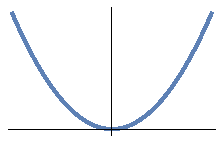
\includegraphics[width=\linewidth]{figures/parabola-1-1.pdf}}

更一般地, 对一个 (可能是无限的) 多项式集合, 可以研究 $\mathbb{A}^{n}$ 中使集合内每个多项式都为零的点所成的集合.

\begin{Definition}{零点集}\leavevmode\label{def:vanishing-set}
  设 $S\subseteq K[x_{1},\ldots,x_{n}]$ 是一个多项式集合. $S$ 的\textbf{零点集}为
  \[
    \mathcal{V}(S)=\{(a_{1},\ldots,a_{n})\in\mathbb{A}^{n}\mid
      f(a_{1},\ldots,a_{n})=0 \text{ 对所有 } f\in S\}\subseteq\mathbb{A}^{n}.
  \]
\end{Definition}

通常称 $\mathcal{V}(S)$ 中的点为 $S$ 中多项式的解. 当 $S=\{f_{1},\ldots,f_{r}\}$ 是有限集时, 我们写 $\mathcal{V}(f_{1},\ldots,f_{r})$, 而不写 $\mathcal{V}(\{f_{1},\ldots,f_{r}\})$.

\begin{Example}{$\mathbb{A}^{2}_{\mathbb{R}}$ 中的曲线}\leavevmode\label{ex:plane-curves}
  考虑 $S=\{y-x^{2}\}\subseteq K[x,y]$. 那么 $\mathcal{V}(S)=\{(a,a^{2})\mid a\in K\}\subseteq\mathbb{A}^{2}$. 当 $K=\mathbb{R}$ 时, 这就是\hyperref[fig:parabola-vanishing-set]{上面的抛物线}. 类似地, $\mathcal{V}(x^{2}+y^{2}-1)$, $\mathcal{V}(y^{2}-x^{3}-x^{2})$ 和 $\mathcal{V}(y^{2}-(x+1)^{3})$ 是\hyperref[fig:three-plane-curves]{下图}所示的 $\mathbb{A}^{2}_{\mathbb{R}}$ 中的平面曲线.
  \par\smallskip
  {\centering\phantomsection\label{fig:three-plane-curves}%
    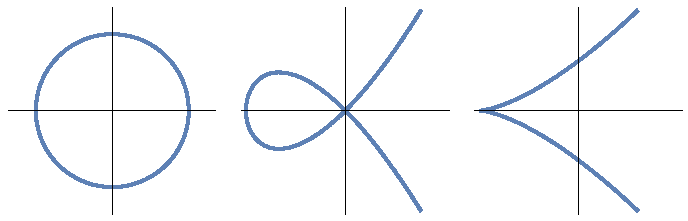
\includegraphics[width=.94\linewidth]{figures/plane-curves-1-3.pdf}\par}
\end{Example}

\begin{Example}{$\mathbb{A}^{3}_{\mathbb{R}}$ 中的曲面}\leavevmode\label{ex:three-surfaces}
  零点集 $\mathcal{V}(x^{2}+y^{2}+z^{2}-1)$, $\mathcal{V}(x^{2}+y^{2}-z^{2})$ 和 $\mathcal{V}(x^{2}+y^{2}z)$ 分别是单位球面, 圆锥面以及\textquotedbl{}Whitney 伞\textquotedbl{}, 如\hyperref[fig:sphere-cone-and-whitney-umbrella]{下图}在 $\mathbb{A}^{3}_{\mathbb{R}}$ 中所示.
  \par\smallskip
  {\centering\phantomsection\label{fig:sphere-cone-and-whitney-umbrella}%
    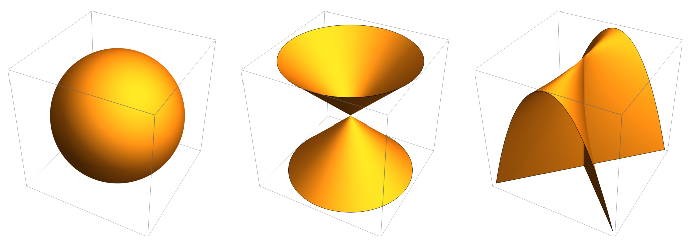
\includegraphics[width=.94\linewidth]{figures/surfaces-1-4.pdf}\par}
\end{Example}

\begin{Example}{坐标轴}\leavevmode\label{ex:vanishing-set-coordinate-axes}
  若 $S=\{xy\}\subseteq K[x,y]$, 则 $\mathcal{V}(S)=\{(a,b)\in\mathbb{A}^{2}\mid ab=0\}\subseteq\mathbb{A}^{2}$. 由于 $K$ 是域, $ab=0$ 当且仅当 $a=0$ 或 $b=0$ (或者两者都为零), 所以 $\mathcal{V}(S)$ 是满足 $a=0$ 的点与满足 $b=0$ 的点的并集. 当 $K=\mathbb{R}$ 时, 这就是实平面 $\mathbb{A}^{2}_{\mathbb{R}}$ 中的 $x$ 轴与 $y$ 轴的并集.
\end{Example}

\begin{Example}{单点}\leavevmode\label{ex:singleton-vanishing-sets}
  令 $S=\{x,y\}\subseteq K[x,y]$. 那么
  \[
    \mathcal{V}(S)=\{(a,b)\in\mathbb{A}^{2}\mid a=0\text{ 且 }b=0\}
      =\{(0,0)\}\subseteq\mathbb{A}^{2}.
  \]
  也就是说, $\mathcal{V}(S)$ 由一个点组成, 即原点.

  类似地, 若 $S=\{x-\mathrm{i},y-1-\mathrm{i},z-5\}\subseteq\mathbb{C}[x,y,z]$, 则
  \[
    \mathcal{V}(S)=\{(\mathrm{i},1+\mathrm{i},5)\}\subseteq\mathbb{A}^{3}_{\mathbb{C}},
  \]
  这同样是一个单点.
\end{Example}

\begin{Example}{$\mathbb{A}^{3}$ 中的一条曲线}\leavevmode\label{ex:space-curve-intersection}
  \BookPairedFigure
    {集合
     \[
       S=\{x^{2}+y^{2}-1,x^{2}-y^{2}-z\}
         \subseteq\mathbb{R}[x,y,z]
     \]
     的零点集由 $\mathbb{A}^{3}_{\mathbb{R}}$ 中使 $a^{2}+b^{2}-1$ 和 $a^{2}-b^{2}-c$ 都为零的点 $(a,b,c)$ 组成. \hyperref[fig:intersection-of-two-surfaces]{图中}将这条曲线画成两个曲面的交, 每个曲面对应一个定义它的多项式.}
    {\phantomsection\label{fig:intersection-of-two-surfaces}%
      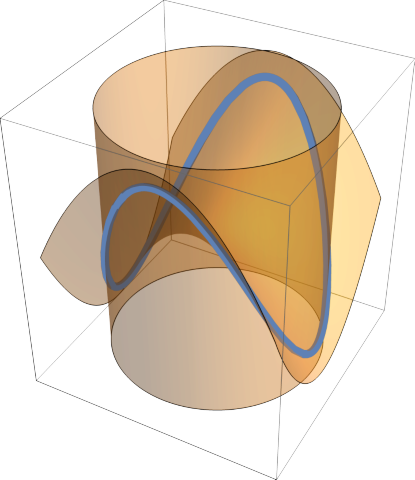
\includegraphics[width=.94\linewidth]{figures/intersection-curve-1-7.png}}
\end{Example}

\BookPairedNoteLeft
  {上面各图的基域都是 $K=\mathbb{R}$. 在 $\mathbb{R}$ 上, 我们有一定的几何直觉; 例如, 大致知道\textquotedbl{}曲线\textquotedbl{}或\textquotedbl{}曲面\textquotedbl{}意味着什么. 代数几何的目标是在一般的域上精确地表述这种直觉.}
  {既然现在把多项式看作函数 $\mathbb{A}^{n}\to K$, 就值得指出多项式与多项式函数之间有一个微妙却重要的区别. 尤其让人有些意外的是, $K[x_{1},\ldots,x_{n}]$ 中不同的多项式可以给出同一个函数 $\mathbb{A}^{n}\to K$.}

例如, 设 $K=\mathbb{F}_{2}=\{0,1\}$, 即含两个元素的域; 回顾一下, 这个域的加法与乘法都是模 $2$ 进行的. 令
\begin{equation}\label{eq:distinct-polynomials-over-two-elements}
  f(x)=1+x+x^{2} \qquad\text{以及}\qquad g(x)=1.
\end{equation}
作为 $\mathbb{F}_{2}[x]$ 的元素, 这两个多项式不相等, 因为它们在单项式 $x$ 和 $x^{2}$ 上的系数不同. 然而, 将它们视作函数 $\mathbb{A}^{1}\to\mathbb{F}_{2}$ 时, 可以看到
\[
  f(0)=1+0+0^{2}=1=g(0) \qquad\text{以及}\qquad
  f(1)=1+1+1^{2}=1=g(1).
\]
因此, 对定义域中的每一个输入, $f$ 和 $g$ 给出同一个输出. 所以尽管它们作为多项式不同, 作为函数却相等.

为了更一般地描述多项式与其对应函数的区别, 令 $K[\mathbb{A}^{n}]$ 表示多项式函数 $\mathbb{A}^{n}\to K$ 的集合. 也就是说, $K[\mathbb{A}^{n}]$ 的元素是形如
\[
  (a_{1},\ldots,a_{n})\mapsto f(a_{1},\ldots,a_{n})
\]
的函数, 其中 $f\in K[x_{1},\ldots,x_{n}]$. 稍加思考即可看出, $K[\mathbb{A}^{n}]$ 在取值于 $K$ 的函数加法与乘法下构成一个环. 把多项式送到其对应函数, 就定义了一个满的环同态 $K[x_{1},\ldots,x_{n}]\to K[\mathbb{A}^{n}]$. 恰好在不同的多项式给出同一个函数时, 这个同态不是单射. 例如,
\[
  \mathbb{F}_{2}[x]\to\mathbb{F}_{2}[\mathbb{A}^{1}]
\]
不是单射, 因为 \eqref{eq:distinct-polynomials-over-two-elements} 中定义的不同多项式 $f,g\in\mathbb{F}_{2}[x]$ 在 $\mathbb{F}_{2}[\mathbb{A}^{1}]$ 中给出同一个多项式函数.

下面的结果表明, 上述现象仅在有限域中出现, 因而只要假定 $K$ 是无限域, 就不必担心这一细微差别.

\begin{Proposition}{多项式与函数}\leavevmode\label{prop:polynomial-function-isomorphism}
  将多项式送到对应函数的环同态 $K[x_{1},\ldots,x_{n}]\to K[\mathbb{A}^{n}]$ 是同构, 当且仅当 $K$ 是无限域.
\end{Proposition}

\begin{Proof}
  我们证明这个充要条件的两个方向.

  ($\Rightarrow$) 用逆否命题来证明. 假设 $K=\{a_{1},\ldots,a_{n}\}$ 是有限域, 考虑非零多项式
  \[
    f=\prod_{i=1}^{n}(x_{1}-a_{i})\in K[x_{1}]\subseteq K[x_{1},\ldots,x_{n}].
  \]
  把 $K$ 中的任何值代入 $x_{1}$, 都会使一个因子为零. 所以 $f$ 定义了零函数 $\mathbb{A}^{n}\to K$. 这表明 $K[x_{1},\ldots,x_{n}]\to K[\mathbb{A}^{n}]$ 不是同构.

  ($\Leftarrow$) 假设 $K$ 是无限域. 根据定义, $K[x_{1},\ldots,x_{n}]\to K[\mathbb{A}^{n}]$ 是满射. 因此只需证明它是单射, 或者等价地, 证明它的核只含零多项式. 为此对 $n$ 作归纳.

  (归纳起点) 假设 $h\in K[x]$ 定义了零函数 $\mathbb{A}^{1}\to K$. 因为 $K$ 是无限域, 这意味着 $h$ 有无穷多个零点. 根据 Corollary~\ref{cor:polynomial-finite-zeros}, 非零多项式只有有限多个零点, 所以 $h$ 必为零多项式.

  (归纳步骤) 假设 $h\in K[x_{1},\ldots,x_{n}]$ 定义了零函数, 写成
  \[
    h=\sum_{i=0}^{d}h_{i}x_{n}^{i},
  \]
  其中 $h_{i}\in K[x_{1},\ldots,x_{n-1}]$. 对每个 $(a_{1},\ldots,a_{n-1})\in\mathbb{A}^{n-1}$, 一元多项式 $h(a_{1},\ldots,a_{n-1},x_{n})\in K[x_{n}]$ 定义了零函数 $\mathbb{A}^{1}\to K$. 因此, 按照归纳起点中的论证, $h(a_{1},\ldots,a_{n-1},x_{n})$ 是零多项式. 特别地, 对所有 $i$ 都有 $h_{i}(a_{1},\ldots,a_{n-1})=0$. 由于这对每个 $(a_{1},\ldots,a_{n-1})\in\mathbb{A}^{n-1}$ 都成立, 所以对所有 $i$, $h_{i}:\mathbb{A}^{n-1}\to K$ 都是零函数. 根据归纳假设, 对每个 $i$, $h_{i}\in K[x_{1},\ldots,x_{n-1}]$ 都是零多项式, 从而 $h$ 是零多项式.
\end{Proof}

\BookExerciseHeading
\begin{BookExercises}
  \item\label{ex:sketch-vanishing-sets} 画出下列零点集的草图.
    \begin{enumerate}[label=(\alph*)]
      \item $\mathcal{V}(x^{2}-1)\subseteq\mathbb{A}^{1}_{\mathbb{R}}$
      \item $\mathcal{V}(x^{2}-y^{2})\subseteq\mathbb{A}^{2}_{\mathbb{R}}$
      \item $\mathcal{V}(y-x^{2},y-x)\subseteq\mathbb{A}^{2}_{\mathbb{R}}$
      \item $\mathcal{V}(x^{2}+y^{2}+z^{2}-1,z)\subseteq\mathbb{A}^{3}_{\mathbb{R}}$
      \item $\mathcal{V}(x^{2}+y^{2}-z^{2},x)\subseteq\mathbb{A}^{3}_{\mathbb{R}}$
      \item $\mathcal{V}(x^{2}+y^{2}-z^{2},z)\subseteq\mathbb{A}^{3}_{\mathbb{R}}$
      \item $\mathcal{V}(xy-y^{2},x^{2}-xy-x+y)\subseteq\mathbb{A}^{2}_{\mathbb{R}}$
    \end{enumerate}
  \item\label{ex:express-sets-by-polynomials} 把下列集合表示成某个 $S$ 的零点集 $\mathcal{V}(S)$.
    \begin{enumerate}[label=(\alph*)]
      \item $\{0,\pi,-1\}\subseteq\mathbb{A}^{1}_{\mathbb{R}}$
      \item $\mathbb{A}^{3}_{\mathbb{R}}$ 中的 $x$ 轴
      \item $\{(4,-1,3)\}\subseteq\mathbb{A}^{3}_{\mathbb{R}}$
      \item $\{(-1,0),(1,0)\}\subseteq\mathbb{A}^{2}_{\mathbb{R}}$
      \item $\{(a,a,a)\mid a\in\mathbb{R}\}\subseteq\mathbb{A}^{3}_{\mathbb{R}}$
      \item $\{(\cos(a),\sin(a),\cos^{2}(a)-\sin^{2}(a))\mid a\in[0,2\pi)\}\subseteq\mathbb{A}^{3}_{\mathbb{R}}$
    \end{enumerate}
  \item\label{ex:origin-over-real-or-complex} 证明: 当 $K=\mathbb{R}$ 时, 原点 $\{(0,0)\}\subseteq\mathbb{A}^{2}_{K}$ 是单个多项式的零点集; 当 $K=\mathbb{C}$ 时则不是.
  \item\label{ex:union-and-intersection-of-vanishing-sets} 设 $f,g\in K[x_{1},\ldots,x_{n}]$. 证明:
    \begin{enumerate}[label=(\alph*)]
      \item $\mathcal{V}(fg)=\mathcal{V}(f)\cup\mathcal{V}(g)$;
      \item $\mathcal{V}(f,g)=\mathcal{V}(f)\cap\mathcal{V}(g)$.
    \end{enumerate}
  \item\label{ex:decompose-a-space-vanishing-set} 设
    \[
      X=\mathcal{V}(x^{2}-yz,xz-x)\subseteq\mathbb{A}^{3}_{K}.
    \]
    \begin{enumerate}[label=(\alph*)]
      \item 证明
        \[
          X=\mathcal{V}(x,y)\cup\mathcal{V}(x,z)\cup\mathcal{V}(x^{2}-y,z-1).
        \]
      \item 利用 (a) 画出 $K=\mathbb{R}$ 时 $X$ 的草图.
    \end{enumerate}
  \item\label{ex:finite-set-affine-line} 对任意域 $K$, 证明 $\mathbb{A}^{1}_{K}$ 中的每个有限集都可表示成一个多项式的零点集.
  \item\label{ex:finite-set-affine-plane} 对任意域 $K$, 证明 $\mathbb{A}^{2}_{K}$ 中的每个有限集都可表示成两个多项式的零点集.
  \item\label{ex:finite-set-affine-space} 推广前面两道习题: 证明 $\mathbb{A}^{n}_{K}$ 中的每个有限集都可表示成一族 $n$ 个多项式的零点集. (提示: 考虑忘掉最后一个坐标的映射 $\mathbb{A}^{n}\to\mathbb{A}^{n-1}$, 并对 $n$ 作归纳.)
\end{BookExercises}

\section{仿射簇}\label{sec:affine-varieties}

并非 $\mathbb{A}^{n}$ 的每个子集都是某族多项式的零点集. 例如, 设 $X\subseteq\mathbb{A}^{1}_{\mathbb{R}}$ 为全体非零实数的集合:
\[
  X=\{a\in\mathbb{R}\mid a\ne0\}\subsetneq\mathbb{A}^{1}_{\mathbb{R}}.
\]
我们来说明 $X$ 不能是任何多项式集合的零点集. 反设对某个集合 $S\subseteq\mathbb{R}[x]$, 有 $X=\mathcal{V}(S)$. 那么 $S$ 必须至少包含一个非零元素, 因为如果 $S$ 是 $\varnothing$ 或 $\{0\}$, 它的零点集就是整个 $\mathbb{A}^{1}_{\mathbb{R}}$. 取 $S$ 中任一个非零元素 $f$. 由于 $X=\mathcal{V}(S)$, 对所有 $a\in\mathbb{R}\setminus\{0\}$ 都有 $f(a)=0$. 这意味着 $f\in\mathbb{R}[x]$ 是一个有无穷多个零点的非零多项式, 与 Corollary~\ref{cor:polynomial-finite-zeros} 矛盾.

鉴于这类例子, 我们给仿射空间中能定义为一个多项式集合的零点集的那些特殊子集起一个名字.

\begin{Definition}{仿射簇}\leavevmode\label{def:affine-variety}
  若对某个多项式集合 $S\subseteq K[x_{1},\ldots,x_{n}]$, 有 $X=\mathcal{V}(S)$, 则称子集 $X\subseteq\mathbb{A}^{n}$ 为\textbf{仿射簇}.
\end{Definition}

我们已经在第~\ref{sec:vanishing-set-operator}~节给出的例子中见过若干仿射簇. 此外, 对第~\ref{sec:vanishing-set-operator}~节中的每个仿射簇, 我们都给出了一个以它为零点集的多项式集合. 另外两个例子可能比前面的任何例子都更基本, 却同样重要: 空集和整个仿射空间.

\begin{Example}{空集和仿射空间都是仿射簇}\leavevmode\label{ex:empty-and-full-affine-varieties}
  常数多项式 $1\in K[x_{1},\ldots,x_{n}]$ 在 $\mathbb{A}^{n}$ 的任一点都不为零, 所以
  \[
    \mathcal{V}(1)=\varnothing\subseteq\mathbb{A}^{n}.
  \]
  零多项式 $0\in K[x_{1},\ldots,x_{n}]$ 在 $\mathbb{A}^{n}$ 的每一点都为零, 所以
  \[
    \mathcal{V}(0)=\mathbb{A}^{n}.
  \]
  因而 $\varnothing$ 和 $\mathbb{A}^{n}$ 都是仿射簇.
\end{Example}

只要写出一些多项式集合, 再考察它们的零点集, 就很容易列出无穷多个仿射簇的例子, 不过这种做法并不能说明太多问题. 更微妙的任务是弄清仿射簇在仿射空间的子集中有什么特别之处. 换句话说, 哪些仿射空间的子集不是仿射簇? 我们已经见过一个例子: $\mathbb{R}\setminus\{0\}$ 不是 $\mathbb{A}^{1}_{\mathbb{R}}$ 中的仿射簇. 事实上, $\mathbb{A}^{1}$ 中仅有的仿射簇是有限点集 (包括 $\varnothing$) 和整个 $\mathbb{A}^{1}$ (Exercise~\ref{ex:affine-varieties-on-the-line}).

另一方面, $\mathbb{A}^{2}$ 中的无限真子集完全可以是仿射簇, $\mathbb{A}^{2}_{\mathbb{R}}$ 中的抛物线就是一例. 但 $\mathbb{A}^{2}_{\mathbb{R}}$ 的真子集要成为仿射簇, 就不可能有非空内部. 下面的例子说明这一现象.

\begin{Example}{实心正方形不是仿射簇}\leavevmode\label{ex:solid-square-not-affine-variety}
  设 $X$ 是 $\mathbb{A}^{2}_{\mathbb{R}}$ 中如下定义的实心正方形:
  \[
    X=\{(a,b)\in\mathbb{A}^{2}_{\mathbb{R}}\mid-1\leq a\leq1
      \text{ 且 }-1\leq b\leq1\}.
  \]
  反设对某个集合 $S\subseteq\mathbb{R}[x,y]$, 有 $X=\mathcal{V}(S)$. 任取 $f\in S$, 我们来说明 $f$ 是零多项式. 写成
  \[
    f=\sum_{i=0}^{d}f_{i}y^{i},
  \]
  其中对每个 $i$ 都有 $f_{i}\in\mathbb{R}[x]$. 由于 $f\in S$, 它在 $X$ 的所有点上都为零. 换句话说, 对任意 $a\in[-1,1]$, 一元多项式
  \[
    f(a,y)=\sum_{i=0}^{d}f_{i}(a)y^{i}\in\mathbb{R}[y]
  \]
  在所有 $b\in[-1,1]$ 处都为零. 由于非零一元多项式只能有有限多个零点, 可知 $f(a,y)$ 必为零多项式, 从而对所有 $i$ 都有 $f_{i}(a)=0$. 换句话说, 我们已经说明一元多项式 $f_{i}\in\mathbb{R}[x]$ 在所有 $a\in[-1,1]$ 处都为零. 再次利用非零一元多项式只有有限多个零点这一事实, 可知对每个 $i$, $f_{i}$ 都是零多项式, 所以 $f$ 是零多项式. 这一论证表明, $S$ 中可能有的多项式只有零多项式, 从而 $X=\mathcal{V}(S)=\mathbb{A}^{2}_{\mathbb{R}}$, 矛盾.

  学过拓扑学的学生不妨证明一个更一般的结论: 赋予 $\mathbb{A}^{n}_{\mathbb{R}}$ 欧氏拓扑后, $\mathbb{A}^{n}_{\mathbb{R}}$ 中唯一具有非空拓扑内部的仿射簇是整个 $\mathbb{A}^{n}_{\mathbb{R}}$ (Exercise~\ref{ex:affine-variety-empty-interior}).
\end{Example}

\begin{Example}{$\mathbb{A}^{2}_{\mathbb{R}}$ 中 $e^{x}$ 的图像不是仿射簇}\leavevmode\label{ex:exponential-graph-not-affine-variety}
  令 $X$ 为实数上的指数函数的图像:
  \begin{equation}\label{eq:exponential-graph}
    X=\{(a,b)\in\mathbb{A}^{2}_{\mathbb{R}}\mid b=e^{a}\}\subseteq\mathbb{A}^{2}_{\mathbb{R}}.
  \end{equation}
  Exercise~\ref{ex:prove-exponential-graph-not-affine-variety} 给出了证明 $X$ 不是仿射簇的严谨思路. 直观上, $X$ 不是仿射簇似乎是合理的: 它由表达式 $y-e^{x}$ 为零来定义, 而这个表达式不是 $x$ 和 $y$ 的多项式. 不过, 采用这种推理时要谨慎. 例如, 表达式 $\sin^{2}(x)+\cos^{2}(x)+y$ 也不是多项式, 但集合
  \[
    \{(a,b)\in\mathbb{A}^{2}_{\mathbb{R}}\mid\sin^{2}(a)+\cos^{2}(a)+b=0\}
    \subseteq\mathbb{A}^{2}_{\mathbb{R}}
  \]
  与集合
  \[
    \{(a,b)\in\mathbb{A}^{2}_{\mathbb{R}}\mid1+b=0\}=\mathcal{V}(1+y)
    \subseteq\mathbb{A}^{2}_{\mathbb{R}}
  \]
  相同, 所以它是一个仿射簇.
\end{Example}

不同的集合 $S$ 的 $\mathcal{V}(S)$ 完全可能给出同一个仿射簇. 例如,
\[
  \mathcal{V}(x,y)=\mathcal{V}(x+y,x-y)=\{(0,0)\}\subseteq\mathbb{A}^{2},
\]
读者不难验证这一点. 事实上, 可以用 $S$ 生成的整个理想 $\langle S\rangle\subseteq K[x_{1},\ldots,x_{n}]$ 替换 $S$, 而不改变其零点集.

\begin{Proposition}{仿射簇由理想定义}\leavevmode\label{prop:affine-varieties-defined-by-ideals}
  若 $S\subseteq K[x_{1},\ldots,x_{n}]$ 是一个多项式集合, 则
  \[
    \mathcal{V}(S)=\mathcal{V}(\langle S\rangle).
  \]
\end{Proposition}

\begin{Proof}
  见 Exercise~\ref{ex:prove-ideals-define-affine-varieties}.
\end{Proof}

为了概括本节的讨论, 我们把 $\mathcal{V}$ 算子看成函数
\[
  \mathcal{V}:\{K[x_{1},\ldots,x_{n}]\text{ 的子集}\}
    \longrightarrow\{\mathbb{A}^{n}\text{ 的子集}\}.
\]
这个函数不是满射, 因为 $\mathbb{A}^{n}$ 的子集不全是仿射簇. 但如果把陪域限制为仿射簇, 则根据定义, 它就成为满射:
\[
  \mathcal{V}:\{K[x_{1},\ldots,x_{n}]\text{ 的子集}\}
    \longrightarrow\{\mathbb{A}^{n}\text{ 中的仿射簇}\}.
\]
$\mathcal{V}$ 算子也不是单射, 因为 $K[x_{1},\ldots,x_{n}]$ 的不同子集可以定义同一个仿射簇. 为了使它成为双射, 第一步是利用 Proposition~\ref{prop:affine-varieties-defined-by-ideals}: 可以把定义域限制为理想, 同时保持函数是满射:
\[
  \mathcal{V}:\{K[x_{1},\ldots,x_{n}]\text{ 的理想}\}
    \longrightarrow\{\mathbb{A}^{n}\text{ 中的仿射簇}\}.
\]
事实上, 这个算子仍不是单射 (见 Exercise~\ref{ex:distinct-ideals-same-variety}). 要最终得到一个双射的 $\mathcal{V}$ 算子, 还需要进一步限制定义域, 并对基域 $K$ 作一个假设.

\BookExerciseHeading
\begin{BookExercises}
  \item\label{ex:affine-varieties-on-the-line} 证明 $\mathbb{A}^{1}$ 中仅有的仿射簇是有限点集和整个 $\mathbb{A}^{1}$.
  \item\label{ex:prove-ideals-define-affine-varieties} 证明 Proposition~\ref{prop:affine-varieties-defined-by-ideals}.
  \item\label{ex:distinct-ideals-same-variety} 举出不同的理想 $I,J\in K[x]$, 使得 $\mathcal{V}(I)=\mathcal{V}(J)$.
  \item\label{ex:twisted-cubic-is-affine-variety} 求一个多项式集合 $S$, 使得 $X=\mathcal{V}(S)$, 由此证明集合
    \[
      X=\{(a,a^{2},a^{3})\mid a\in K\}\subseteq\mathbb{A}^{3}
    \]
    是一个仿射簇. (簇 $X$ 称为仿射扭三次曲线.)
  \item\label{ex:containment-in-affine-plane} 设 $K$ 是无限域. $\mathbb{A}^{3}_{K}$ 中的一个平面是能定义为某个非常数线性多项式的零点集的仿射簇 $P$:
    \[
      P=\mathcal{V}(Ax+By+Cz+D),
    \]
    其中 $A,B,C,D\in K$, 且 $A,B,C$ 不全为零. 证明下列结论.
    \begin{enumerate}[label=(\alph*)]
      \item 对任意次数至多为二的多项式 $f_{1},f_{2},f_{3}\in K[x]$, 集合
        \[
          X=\{(f_{1}(a),f_{2}(a),f_{3}(a))\mid a\in K\}\subseteq\mathbb{A}^{3}
        \]
        至少包含在一个平面内. (提示: 对 $A,B,C,D$ 建立线性方程, 并说明至少存在一个解.)
      \item Exercise~\ref{ex:twisted-cubic-is-affine-variety} 中的仿射扭三次曲线不包含在任何平面内. (因此, 把 (a) 中的\textquotedbl{}二\textquotedbl{}换成\textquotedbl{}三\textquotedbl{}后, 结论不成立.)
    \end{enumerate}
  \item\label{ex:parameterized-set-not-affine-variety} 设 $K$ 是无限域. 证明集合
    \[
      X=\{(a,ab)\mid a,b\in K\}\subseteq\mathbb{A}^{2}
    \]
    不是仿射簇.
  \item\label{ex:prove-exponential-graph-not-affine-variety} 证明表达式 $y-e^{x}$ 在 $\mathbb{A}^{2}_{\mathbb{R}}$ 中的零点集 $X$ 不是仿射簇, 可以采用以下策略.
    \begin{enumerate}[label=(\alph*)]
      \item 反设对某个 $S\subseteq\mathbb{R}[x,y]$, 有 $X=\mathcal{V}(S)$. 说明为什么存在非零多项式 $f\in\mathbb{R}[x,y]$, 使得对所有 $a\in\mathbb{R}$ 都有 $f(a,e^{a})=0$.
      \item 对上述任意多项式 $f$, 写成
        \[
          f(x,y)=p_{0}(x)+p_{1}(x)y+p_{2}(x)y^{2}+\cdots+p_{d}(x)y^{d},
        \]
        其中 $p_{d}\ne0\in\mathbb{R}[x]$. 证明对所有 $a\in\mathbb{R}$ 都有
        \[
          \frac{p_{0}(a)}{e^{da}}+\frac{p_{1}(a)}{e^{(d-1)a}}+
          \frac{p_{2}(a)}{e^{(d-2)a}}+\cdots+
          \frac{p_{d-1}(a)}{e^{a}}+p_{d}(a)=0.
        \]
      \item 令 $a\to\infty$, 取上式的极限, 得到
        \[
          \lim_{a\to\infty}p_{d}(a)=0.
        \]
        说明对任意非零的 $g\in\mathbb{R}[x]$, 有 $\lim g(a)\ne0$, 从而得出矛盾.
    \end{enumerate}
  \item\label{ex:affine-variety-empty-interior} (供学过一些拓扑学的学生.) 把 $\mathbb{A}^{n}_{\mathbb{R}}=\mathbb{R}^{n}$ 看作带欧氏拓扑的拓扑空间. 设 $X\subseteq\mathbb{A}^{n}_{\mathbb{R}}$ 是一个不同于 $\mathbb{A}^{n}_{\mathbb{R}}$ 本身的仿射簇. 证明: 作为 $\mathbb{A}^{n}_{\mathbb{R}}$ 的拓扑子空间, $X$ 的内部为空. (用类似的证明, 把 $\mathbb{R}$ 换成 $\mathbb{C}$ 后, 同一结果也成立.)
\end{BookExercises}

\section{\texorpdfstring{$\mathcal{I}$}{I} 算子}\label{sec:vanishing-ideal-operator}

在第~\ref{sec:vanishing-set-operator}~节, 我们学习了怎样借助 $\mathcal{V}$ 算子, 给 $K[x_{1},\ldots,x_{n}]$ 的每个子集对应 $\mathbb{A}^{n}$ 的一个子集. 在本节中, 我们反过来描述一个算子, 给 $\mathbb{A}^{n}$ 的每个子集对应 $K[x_{1},\ldots,x_{n}]$ 的一个子集.

\begin{Definition}{消没理想}\leavevmode\label{def:vanishing-ideal}
  设 $X\subseteq\mathbb{A}^{n}$ 是一个子集. $X$ 的\textbf{消没理想}定义为
  \[
    \mathcal{I}(X)=\{f\in K[x_{1},\ldots,x_{n}]
      \mid f(a_{1},\ldots,a_{n})=0\text{ 对所有 }(a_{1},\ldots,a_{n})\in X\}.
  \]
\end{Definition}

换句话说, $X$ 的消没理想是所有在 $X$ 上处处为零的多项式所成的集合. 正如名称所暗示的那样, 集合 $\mathcal{I}(X)$ 不只是多项式环 $K[x_{1},\ldots,x_{n}]$ 的一个子集, 还是一个理想 (Exercise~\ref{ex:vanishing-set-of-polynomials-is-ideal}).

\begin{Example}{在 $(0,0)$ 处为零的多项式}\leavevmode\label{ex:vanishing-ideal-of-origin}
  设 $X=\{(0,0)\}\subseteq\mathbb{A}^{2}$. 多项式 $f\in K[x,y]$ 在 $(0,0)$ 处为零, 当且仅当 $f$ 的常数项为零. 如 Example~\ref{ex:vanishing-constant-ideal} 所述, 所有这样的多项式构成理想 $\langle x,y\rangle$. 因此, $\mathcal{I}(X)=\langle x,y\rangle$.
\end{Example}

\begin{Example}{一元情形中的消没理想}\leavevmode\label{ex:one-variable-vanishing-ideals}
  设 $X=\{1,3\}\subseteq\mathbb{A}^{1}_{\mathbb{R}}$. 根据 Corollary~\ref{cor:polynomial-factor-theorem}, 多项式 $f\in\mathbb{R}[x]$ 在 $1$ 处为零, 当且仅当 $x-1$ 整除 $f$; $f$ 在 $3$ 处为零, 当且仅当 $x-3$ 整除 $f$. 由于 $x-1$ 和 $x-3$ 都不可约, 由 $\mathbb{R}[x]$ 中分解的唯一性可得
  \[
    \mathcal{I}(X)=\{f\in\mathbb{R}[x]\mid(x-1)(x-3)\text{ 整除 }f\}
    =\langle x^{2}-4x+3\rangle.
  \]
  采用类似方法可求任意 $X\subseteq\mathbb{A}^{1}$ 的消没理想 (Exercise~\ref{ex:vanishing-ideals-of-subsets-of-line}).
\end{Example}

\begin{Example}{抛物线的消没理想}\leavevmode\label{ex:vanishing-ideal-of-parabola}
  设 $K$ 是无限域, 并设 $X$ 为下式定义的仿射簇:
  \[
    X=\mathcal{V}(y-x^{2})=\{(a,a^{2})\mid a\in K\}\subseteq\mathbb{A}^{2}.
  \]
  哪些多项式在 $X$ 的每个点都为零? 任何形如 $(y-x^{2})f(x,y)$ 的多项式当然在 $X$ 的每个点都为零, 所以 $\langle y-x^{2}\rangle\subseteq\mathcal{I}(X)$. 下面证明反向的包含关系也成立.

  设 $f\in\mathcal{I}(X)$. Example~\ref{ex:quotient-parabola-computations} 中的论证表明, 在商环 $K[x,y]/\langle y-x^{2}\rangle$ 中, 有 $[f(x,y)]=[f(x,x^{2})]$. 特别地, 这意味着
  \begin{equation}\label{eq:parabola-vanishing-ideal-difference}
    f(x,y)-f(x,x^{2})\in\langle y-x^{2}\rangle.
  \end{equation}
  由 $f$ 在 $X=\{(a,a^{2})\mid a\in K\}$ 上处处为零的假设可知, 对每个 $a\in K$ 都有 $f(a,a^{2})=0$. 这意味着 $f(x,x^{2})\in K[x]$ 是一个具有无穷多个零点的一元多项式. 只有在 $f(x,x^{2})$ 为零多项式时这才可能. 将 $f(x,x^{2})=0$ 代入 \eqref{eq:parabola-vanishing-ideal-difference}, 可知 $f\in\langle y-x^{2}\rangle$, 从而有 $\mathcal{I}(X)\subseteq\langle y-x^{2}\rangle$.

  两个方向的包含关系都已证明, 因此 $\mathcal{I}(X)=\langle y-x^{2}\rangle$.
\end{Example}

即使在 Example~\ref{ex:vanishing-ideal-of-parabola} 的抛物线这样简单的情形中, 证明消没理想等于 $\langle y-x^{2}\rangle$ 也已经颇费周折. 的确, 一般来说, 计算仿射簇的消没理想并不容易, 通常必须针对每个具体情形采用专门的方法 (更多此类计算的例子见 Exercises~\ref{ex:vanishing-ideals-of-subsets-of-line}--\ref{ex:unit-circle-infinite-field}). 如第~\ref{sec:nullstellensatz}~节所示, 零点定理会大大简化计算消没理想的工作.

现在我们已经介绍了 $\mathcal{V}$ 和 $\mathcal{I}$ 算子, 它们把 $K[x_{1},\ldots,x_{n}]$ 的子集与 $\mathbb{A}^{n}$ 的子集相互联系起来. 自然会问, 这两个算子在多大程度上互为逆运算? 下面的结果给出第一个答案: 在一般情形下, 它们不互为逆运算; 但把它们限制在消没理想和仿射簇上以后, 它们就互为逆运算了.

\begin{Proposition}{复合 $\mathcal{V}$ 和 $\mathcal{I}$ 算子}\leavevmode\label{prop:compose-vanishing-operators}
  \strut\par\nopagebreak[4]
  \begin{enumerate}[label=\arabic*.,ref=\arabic*]
    \item\label{item:compose-vanishing-operators-sets} 设 $X\subseteq\mathbb{A}^{n}$. 则
    \[
      \mathcal{V}(\mathcal{I}(X))\supseteq X,
    \]
    等号成立当且仅当对某个 $S\subseteq K[x_{1},\ldots,x_{n}]$, 有 $X=\mathcal{V}(S)$.
    \item\label{item:compose-vanishing-operators-polynomials} 设 $S\subseteq K[x_{1},\ldots,x_{n}]$. 则
    \[
      \mathcal{I}(\mathcal{V}(S))\supseteq S,
    \]
    等号成立当且仅当对某个 $X\subseteq\mathbb{A}^{n}$, 有 $S=\mathcal{I}(X)$.
  \end{enumerate}
\end{Proposition}

\begin{Proof}
  我们证明第~\ref{item:compose-vanishing-operators-sets}~部分, 第~\ref{item:compose-vanishing-operators-polynomials}~部分留给 Exercise~\ref{ex:prove-second-composition-inclusion}.

  取 $a=(a_{1},\ldots,a_{n})\in X$. 为证明 $a\in\mathcal{V}(\mathcal{I}(X))$, 任取多项式 $f\in\mathcal{I}(X)$. 根据消没理想的定义, 对所有 $b\in X$ 都有 $f(b)=0$. 特别地, $f(a)=0$. 这样便证明了对每个 $f\in\mathcal{I}(X)$ 都有 $f(a)=0$. 这意味着 $a\in\mathcal{V}(\mathcal{I}(X))$.

  若等号成立, 则 $X$ 是 $S=\mathcal{I}(X)$ 的零点集, 这就证明了充要条件的一个方向. 为了证明反向, 设对某个 $S\subseteq K[x_{1},\ldots,x_{n}]$, 有 $X=\mathcal{V}(S)$. 必须证明 $\mathcal{V}(\mathcal{I}(X))\subseteq X$. 这等价于证明 $a\notin X$ 蕴含 $a\notin\mathcal{V}(\mathcal{I}(X))$, 所以假定 $a\notin X$. 由于 $X=\mathcal{V}(S)$ 且 $a\notin X$, 存在某个 $f\in S$ 使得 $f(a)\ne0$. 又因为 $f\in S$ 且 $X=\mathcal{V}(S)$, $f$ 在 $X$ 上处处为零, 所以 $f\in\mathcal{I}(X)$. 由 $f\in\mathcal{I}(X)$ 且 $f(a)\ne0$, 可知 $a\notin\mathcal{V}(\mathcal{I}(X))$.
\end{Proof}

\BookPairedNoteLeft
  {若 $X\subseteq\mathbb{A}^{n}$ 是仿射簇, 该命题的第~\ref{item:compose-vanishing-operators-sets}~部分说明有一个以 $X$ 为零点集的特别的理想, 即 $\mathcal{I}(X)$.}
  {若 $X\subseteq\mathbb{A}^{n}$ 是一个子集, Proposition~\ref{prop:compose-vanishing-operators} 第一部分中的集合 $\mathcal{V}(\mathcal{I}(X))$ 还有另一种解释: 它是包含 $X$ 的最小仿射簇 (Exercise~\ref{ex:smallest-affine-variety-containing-set}). 从这个意义上说, 它类似于由集合 $S$ 生成的理想, 即包含 $S$ 的最小理想.}
\noindent 我们甚至可以称 $\mathcal{V}(\mathcal{I}(X))$ 为\textquotedbl{}由 $X$ 生成的仿射簇\textquotedbl{}, 并记作 $\langle X\rangle$. 用这个记号, Proposition~\ref{prop:compose-vanishing-operators} 的最后一部分就与 Proposition~\ref{prop:affine-varieties-defined-by-ideals} 相类似:
\[
  \mathcal{I}(X)=\mathcal{I}(\langle X\rangle).
\]

从 Proposition~\ref{prop:compose-vanishing-operators} 的两个充要条件可以看出, 这些包含关系当然可能是严格的. 例如, 若 $X$ 不是仿射簇, 则对任意 $S$ 都有 $X\ne\mathcal{V}(S)$, 因而 $X\ne\mathcal{V}(\mathcal{I}(X))$. 同样, 若 $S$ 不是理想, 就不可能有 $S=\mathcal{I}(\mathcal{V}(S))$, 因为后者是理想. 事实上, 即使 $S$ 是理想, 等号也不必成立. 下面的例子说明这一点.

\begin{Example}{$\mathcal{I}(\mathcal{V}(I))\ne I$}\leavevmode\label{ex:square-ideal-not-vanishing-ideal}
  设 $I=\langle x^{2}\rangle\subseteq K[x]$. 则
  \[
    \mathcal{V}(I)=\{a\in K\mid a^{2}=0\}.
  \]
  因为 $K$ 是域, 所以 $a^{2}=0$ 当且仅当 $a=0$. 因此, $\mathcal{V}(I)=\{0\}$. 与 Example~\ref{ex:one-variable-vanishing-ideals} 相同的推理表明 $\mathcal{I}(\{0\})=\langle x\rangle$, 所以
  \[
    \mathcal{I}(\mathcal{V}(I))=\mathcal{I}(\{0\})=\langle x\rangle.
  \]
  消没理想 $\mathcal{I}(\mathcal{V}(I))=\langle x\rangle$ 包含 $I=\langle x^{2}\rangle$, 但不等于它. 因此, 根据 Proposition~\ref{prop:compose-vanishing-operators} 第二部分中的充要条件, $I$ 不是任何 $X\subseteq\mathbb{A}^{1}$ 的消没理想.
\end{Example}

在第~\ref{sec:affine-varieties}~节末尾, 我们看到 $\mathcal{V}$ 算子给出满射
\[
  \mathcal{V}:\{K[x_{1},\ldots,x_{n}]\text{ 中的理想}\}
    \longrightarrow\{\mathbb{A}^{n}\text{ 中的仿射簇}\}.
\]
由 Proposition~\ref{prop:compose-vanishing-operators} 可知, 若把定义域限制为消没理想的集合, 即那些能作为某个集合的消没理想的理想, 那么 $\mathcal{V}$ 算子就成为双射, 其逆由 $\mathcal{I}$ 算子给出. 因此, 要理解代数与几何之间的这本词典, 我们的目标就是更好地理解 $K[x_{1},\ldots,x_{n}]$ 中的消没理想. 受 Example~\ref{ex:square-ideal-not-vanishing-ideal} 中观察的启发, 下一节将介绍根理想这一代数概念, 沿这个方向迈出第一步.

\BookExerciseHeading
\begin{BookExercises}
  \item\label{ex:vanishing-set-of-polynomials-is-ideal} 对任意子集 $X\subseteq\mathbb{A}^{n}$, 证明 $\mathcal{I}(X)\subseteq K[x_{1},\ldots,x_{n}]$ 是一个理想.
  \item\label{ex:prove-second-composition-inclusion} 证明 Proposition~\ref{prop:compose-vanishing-operators} 第~\ref{item:compose-vanishing-operators-polynomials}~部分.
  \item\label{ex:vanishing-ideals-of-subsets-of-line} 设 $X\subseteq\mathbb{A}^{1}$.
    \begin{enumerate}[label=(\alph*)]
      \item 假设 $X=\{a_{1},\ldots,a_{r}\}$ 是有限集. 利用 $K[x]$ 中分解的唯一性证明
        \[
          \mathcal{I}(X)=\langle(x-a_{1})\cdots(x-a_{r})\rangle\subseteq K[x].
        \]
      \item 假设 $X$ 是无限集. 证明 $\mathcal{I}(X)=\langle0\rangle$.
    \end{enumerate}
  \item\label{ex:vanishing-ideal-quadratic-real-complex} 分别求 $\mathcal{V}(x^{2}+1)\subseteq\mathbb{A}^{1}$ 的消没理想:
    \begin{enumerate}[label=(\alph*)]
      \item 在 $\mathbb{R}$ 上;
      \item 在 $\mathbb{C}$ 上.
    \end{enumerate}
  \item\label{ex:vanishing-ideal-of-a-single-point} 设 $X=\{(a_{1},\ldots,a_{n})\}\in\mathbb{A}^{n}$ 是一个单点. 证明
    \[
      \mathcal{I}(X)=\langle x_{1}-a_{1},\ldots,x_{n}-a_{n}\rangle.
    \]
  \item\label{ex:vanishing-ideal-of-real-unit-circle} 设 $X=\mathcal{V}(x^{2}+y^{2}-1)\subseteq\mathbb{A}^{2}_{\mathbb{R}}$ 是单位圆. 这道习题证明 $\mathcal{I}(X)=\langle x^{2}+y^{2}-1\rangle$.
    \begin{enumerate}[label=(\alph*)]
      \item 证明 $\mathcal{I}(X)\supseteq\langle x^{2}+y^{2}-1\rangle$.
      \item 证明 $\mathcal{I}(X)\subseteq\langle x^{2}+y^{2}-1\rangle$, 可以采用以下证明提纲. 假设 $f\in\mathcal{I}(X)$.
        \begin{enumerate}[label=\roman*.]
          \item 证明对某些 $g_{1},g_{2}\in\mathbb{R}[x]$, 有
            \[
              f-g_{1}-yg_{2}\in\langle x^{2}+y^{2}-1\rangle.
            \]
          \item 利用 $f\in\mathcal{I}(X)$ 证明对所有 $a\in[-1,1]$, 都有
            \[
              g_{1}(a)^{2}=(1-a^{2})g_{2}(a)^{2},
            \]
            并得出 $g_{1}(x)^{2}=(1-x^{2})g_{2}(x)^{2}$.
          \item 利用分解的唯一性证明 $g_{1}$ 和 $g_{2}$ 都是零多项式, 由此得到 $f\in\langle x^{2}+y^{2}-1\rangle$.
        \end{enumerate}
    \end{enumerate}
  \item\label{ex:vanishing-ideal-of-unit-n-sphere} 设 $X=\mathcal{V}(x_{1}^{2}+\cdots+x_{n}^{2}-1)\subseteq\mathbb{A}^{n}_{\mathbb{R}}$ 是单位 $n$ 维球面. 推广上一道习题, 证明 $\mathcal{I}(X)=\langle x_{1}^{2}+\cdots+x_{n}^{2}-1\rangle$.
  \item\label{ex:unit-circle-infinite-field} 设 $K$ 是满足 $1\ne-1$ 的无限域, 且 $X=\mathcal{V}(x^{2}+y^{2}-1)\subseteq\mathbb{A}^{2}_{K}$.
    \begin{enumerate}[label=(\alph*)]
      \item 对任意满足 $c^{2}\ne-1$ 的 $c\in K$, 证明
        \[
          \left(\frac{c^{2}-1}{c^{2}+1},\frac{2c}{c^{2}+1}\right)\in X.
        \]
      \item 证明有无穷多个 $a\in K$, 使 $(a,b)\in X$ 对某个 $b\in K$ 成立.
      \item 证明 $\mathcal{I}(X)=\langle x^{2}+y^{2}-1\rangle$, 可以改用 Exercise~\ref{ex:vanishing-ideal-of-real-unit-circle} 的策略来处理本题.
    \end{enumerate}
  \item\label{ex:parabola-vanishing-ideal-over-f2} 设 $K=\mathbb{F}_{2}$ 是含两个元素的有限域. 令
    \[
      X=\mathcal{V}(y-x^{2})\subseteq\mathbb{A}^{2}_{\mathbb{F}_{2}}.
    \]
    证明 $\mathcal{I}(X)\ne\langle y-x^{2}\rangle$, 这与 Example~\ref{ex:vanishing-ideal-of-parabola} 中讨论的 $\mathbb{R}$ 上的类似情形不同. 求 $\mathcal{I}(X)$.
  \item\label{ex:smallest-affine-variety-containing-set} 设 $X\subseteq\mathbb{A}^{n}$ 是任意子集.
    \begin{enumerate}[label=(\alph*)]
      \item 证明 $\mathcal{V}(\mathcal{I}(X))$ 是包含 $X$ 的最小仿射簇, 其含义如下: 若 $Y\subseteq\mathbb{A}^{n}$ 是任意仿射簇, 且 $X\subseteq Y$, 则 $\mathcal{V}(\mathcal{I}(X))\subseteq Y$.
      \item 任选一个不是仿射簇的 $X\subseteq\mathbb{A}^{2}_{\mathbb{R}}$, 计算 $\mathcal{V}(\mathcal{I}(X))$, 以说明 (a).
    \end{enumerate}
\end{BookExercises}

\section{根理想}\label{sec:radical-ideals}

上一节说明了 $K[x_{1},\ldots,x_{n}]$ 中并非每个理想都能作为 $\mathbb{A}^{n}$ 中某个子集的消没理想. 特别地, 在 Example~\ref{ex:square-ideal-not-vanishing-ideal} 中, 我们看到理想 $\langle x^{2}\rangle\subseteq K[x]$ 不是消没理想. 那么, 怎样判断给定的理想是否为某个 $X$ 的 $\mathcal{I}(X)$ 呢? 本节来考察消没理想的一个重要性质: 消没理想都是根理想.

\begin{Definition}{根理想}\leavevmode\label{def:radical-ideal}
  若对所有 $a\in R$ 都有
  \[
    a^{m}\in I\text{ 对某个整数 }m>0\text{ 成立}
    \quad\Longrightarrow\quad a\in I,
  \]
  则称理想 $I\subseteq R$ 为\textbf{根理想}.
\end{Definition}

换句话说, 一个理想是根理想, 当且仅当它对开方封闭: 只要一个元素的某次幂属于理想, 该元素本身就必须属于理想. 注意, Example~\ref{ex:square-ideal-not-vanishing-ideal} 中的理想 $\langle x^{2}\rangle\subseteq K[x]$ 不是根理想, 因为 $x^{2}\in\langle x^{2}\rangle$, 但 $x\notin\langle x^{2}\rangle$. 下面的结果表明, 所有消没理想都具有这个性质.

\begin{Proposition}{消没理想都是根理想}\leavevmode\label{prop:vanishing-ideals-are-radical}
  对任意集合 $X\subseteq\mathbb{A}^{n}$, 消没理想 $\mathcal{I}(X)$ 是根理想.
\end{Proposition}

特别地, 由 Proposition~\ref{prop:vanishing-ideals-are-radical} 和 $\langle x^{2}\rangle$ 不是根理想这一事实可知, $\langle x^{2}\rangle$ 不是消没理想, 正如我们在 Example~\ref{ex:square-ideal-not-vanishing-ideal} 中看到的那样.

\begin{Proof}\unskip\textbf{ of Proposition~\ref{prop:vanishing-ideals-are-radical}}\quad
  设 $X\subseteq\mathbb{A}^{n}$ 是一个子集, 并假设存在正整数 $m$ 使得 $f^{m}\in\mathcal{I}(X)$, 换句话说, 对所有 $a\in X$ 都有 $f^{m}(a)=0$. 那么
  \[
    0=f^{m}(a)=\bigl(f(a)\bigr)^{m}\in K.
  \]
  由于 $K$ 是域, 它没有零因子. 特别地, $\bigl(f(a)\bigr)^{m}=0$ 当且仅当 $f(a)=0$. 因而对所有 $a\in X$, 都有 $f(a)=0$, 所以 $f\in\mathcal{I}(X)$.
\end{Proof}

特别地, Proposition~\ref{prop:vanishing-ideals-are-radical} 表明根理想在代数几何中起核心作用. 因此, 本节余下的篇幅将集中介绍与根理想有关的一些基本概念.

根据定义, 若一个理想对开方不封闭, 它就不是根理想. 因此, 你或许会想到, 只要补上缺少的根, 就能构造一个根理想. 下面的定义将这一构造精确化.

\begin{Definition}{理想的根}\leavevmode\label{def:radical-of-an-ideal}
  设 $I\subseteq R$ 是一个理想. $I$ 的\textbf{根}为
  \[
    \sqrt{I}=\{a\in R\mid a^{m}\in I\text{ 对某个 }m>0\text{ 成立}\}.
  \]
\end{Definition}

如下一个结果所示, 这个\textquotedbl{}补上缺少的根\textquotedbl{}的过程确实给出一个根理想.

\begin{Proposition}{理想的根是根理想}\leavevmode\label{prop:radicals-are-radical}
  若 $I\subseteq R$ 是一个理想, 则 $\sqrt{I}$ 是根理想.
\end{Proposition}

\begin{Proof}
  $\sqrt{I}$ 是一个理想的证明见 Exercise~\ref{ex:radical-is-an-ideal}. 为了证明 $\sqrt{I}$ 是根理想, 假设对某个整数 $k>0$, 有 $a^{k}\in\sqrt{I}$, 需要证明 $a\in\sqrt{I}$. 根据 $\sqrt{I}$ 的定义, 有
  \[
    a^{k}\in\sqrt{I}\quad\Longrightarrow\quad(a^{k})^{m}\in I
      \text{ 对某个整数 }m>0\text{ 成立}.
  \]
  换句话说, $a^{(km)}\in I$, 因而 $a\in\sqrt{I}$.
\end{Proof}

如果 $I$ 是根理想, 那么它已经对开方封闭, 所以 $I=\sqrt{I}$. 反过来, 若 $I=\sqrt{I}$, 则 Proposition~\ref{prop:radicals-are-radical} 蕴含 $I$ 是根理想. 这样我们证明了以下对根理想的有用刻画.

\begin{Corollary}{根理想的刻画}\leavevmode\label{cor:characterize-radical-ideals}
  理想 $I\subseteq R$ 是根理想, 当且仅当 $I=\sqrt{I}$.
\end{Corollary}

下面举几个例子, 帮助读者熟悉根理想.

\begin{Example}{}\leavevmode\label{ex:radical-of-square-variable}
  若 $R=K[x]$ 且 $I=\langle x^{2}\rangle$, 我们已经看到 $I$ 不是根理想. 若要通过加入 $I$ 中元素的所有可能的根来扩大 $I$, 应当加些什么呢? 下面证明
  \[
    \sqrt{I}=\langle x\rangle.
  \]
  首先, 由于 $x^{2}\in I$, 故 $x\in\sqrt{I}$. 因为 $\sqrt{I}$ 是理想, 由 $x\in\sqrt{I}$ 可知 $\langle x\rangle\subseteq\sqrt{I}$, 这就证明了一个方向的包含关系.

  反过来, 假设 $f\notin\langle x\rangle$. 这意味着 $f$ 的常数项非零. 因而对所有整数 $m>0$, $f^{m}$ 的常数项都非零, 所以 $f^{m}\notin I$. 因此 $f\notin\sqrt{I}$, 这就用逆否命题证明了 $\sqrt{I}\subseteq\langle x\rangle$.
\end{Example}

\begin{Example}{}\leavevmode\label{ex:radical-of-twelve}
  若 $R=\mathbb{Z}$ 且 $I=\langle12\rangle$, 那么 $I$ 不是根理想, 因为 $6^{2}\in I$, 但 $6\notin I$. 事实上,
  \[
    \sqrt{I}=\langle6\rangle.
  \]
  为证 $\sqrt{I}\subseteq\langle6\rangle$, 取 $r\in\sqrt{I}$. 则对某个正整数 $m$ 和某个整数 $k$, 有 $r^{m}=12k$. 由于 $2$ 是素数且 $2\mid r^{m}$, 根据 Euclid 引理可得 $2\mid r$. 同理可得 $3\mid r$. 因为 $r$ 同时被 $2$ 和 $3$ 整除, 所以 $r$ 被 $6$ 整除, 即 $r\in\langle6\rangle$, 这就证明了一个方向的包含关系.

  反过来, 若 $r\in\langle6\rangle$, 则对某个整数 $k$, 有 $r=6k$. 因此
  \[
    r^{2}=36k^{2}=12(3k^{2}),
  \]
  所以 $r^{2}\in I$. 由此得 $r\in\sqrt{I}$, 验证了 $\langle6\rangle\subseteq\sqrt{I}$.
\end{Example}

比较上一例中的根理想 $\langle6\rangle$ 和非根理想 $\langle12\rangle$, 可见 $6$ 是无平方因子的, 换句话说, 它不被任何素数的平方整除. 而 $12$ 不是无平方因子的, 它被 $2^{2}$ 整除. 与 Example~\ref{ex:radical-of-twelve} 类似的论证表明, $\langle n\rangle\subseteq\mathbb{Z}$ 是根理想当且仅当 $n$ 无平方因子.

在代数几何的背景下, 能够判断理想 $I\subseteq K[x_{1},\ldots,x_{n}]$ 何时是根理想会很有用. 对一般的理想而言, 这可能相当困难. 不过, 当 $I$ 是主理想时, 情形与整数的情形类似. 为了准确叙述结果, 取非常数多项式 $f\in K[x_{1},\ldots,x_{n}]$, 并考虑其一个不可约分解:
\[
  f=p_{1}\cdots p_{m}.
\]
由不可约性可知, $p_{i}\mid p_{j}$ 当且仅当两者相差一个常数因子. 把相差常数因子的各项归在一起, 可以写成
\begin{equation}\label{eq:distinct-irreducible-factorization}
  f=aq_{1}^{k_{1}}\cdots q_{\ell}^{k_{\ell}}
\end{equation}
其中 $a\in K$ 非零, 每个 $q_{i}$ 都不可约, 且 $i\ne j$ 时 $q_{i}\nmid q_{j}$. 我们称 \eqref{eq:distinct-irreducible-factorization} 为 $f$ 的\textbf{不同不可约因子分解}, 称各 $q_{i}$ 为 $f$ 的\textbf{不同不可约因子}. 由分解的唯一性可知, 除去重新排列和乘以常数的差别, 不同不可约因子是唯一的.

下面的结果用这些因子来描述主理想的根.

\begin{Proposition}{主理想的根}\leavevmode\label{prop:radicals-of-principal-ideals}
  若 $f\in K[x_{1},\ldots,x_{n}]$ 是非常数多项式, 不同不可约因子为 $q_{1},\ldots,q_{\ell}$, 则
  \[
    \sqrt{\langle f\rangle}=\langle q_{1}\cdots q_{\ell}\rangle.
  \]
  特别地, $\langle f\rangle$ 是根理想, 当且仅当 $f$ 不被任何非常数多项式的平方整除.
\end{Proposition}

\begin{Proof}
  我们证明等式两边互相包含, 将充要条件的推导留给 Exercise~\ref{ex:principal-radical-iff-square-free}.

  ($\subseteq$) 假设 $g\in\sqrt{\langle f\rangle}$. 那么对某个 $m>0$ 和某个 $h\in K[x_{1},\ldots,x_{n}]$, 有 $g^{m}=hf$. 特别地, 这意味着对每个 $i$, 都有 $q_{i}\mid g^{m}$. 由不同不可约因子的唯一性可知, 每个 $q_{i}$ 必定是 $g^{m}$ 的不同不可约因子之一. 因为 $g^{m}$ 的不同不可约因子与 $g$ 的相同, 所以每个 $q_{i}$ 也必定是 $g$ 的不同不可约因子之一. 从而 $q_{1}\cdots q_{\ell}\mid g$, 所以 $g\in\langle q_{1}\cdots q_{\ell}\rangle$.

  ($\supseteq$) 假设 $g\in\langle q_{1}\cdots q_{\ell}\rangle$, 写成 $g=hq_{1}\cdots q_{\ell}$, 其中 $h$ 为某个多项式. 对于不同不可约因子分解
  \[
    f=aq_{1}^{k_{1}}\cdots q_{\ell}^{k_{\ell}},
  \]
  令 $m=\max\{k_{1},\ldots,k_{\ell}\}$. 于是
  \[
    g^{m}=h^{m}q_{1}^{m}\cdots q_{\ell}^{m}
      =\bigl(h^{m}q_{1}^{m-k_{1}}\cdots q_{\ell}^{m-k_{\ell}}a^{-1}\bigr)f
      \in\langle f\rangle,
  \]
  因而 $g\in\sqrt{\langle f\rangle}$.
\end{Proof}

\begin{Example}{{\textmd{$\langle x^{2}+y^{2}\rangle\subseteq\mathbb{C}[x,y]$} 是根理想}}\leavevmode\label{ex:sum-of-squares-complex-radical}
  $x^{2}+y^{2}$ 在 $\mathbb{C}[x,y]$ 中的不可约分解为
  \[
    x^{2}+y^{2}=(x-\mathrm{i}y)(x+\mathrm{i}y).
  \]
  因为两个不可约因子不同, 所以 $x^{2}+y^{2}$ 无平方因子. 因此, 理想 $\langle x^{2}+y^{2}\rangle\subseteq\mathbb{C}[x,y]$ 是根理想.
\end{Example}

\begin{Example}{不是消没理想的根理想}\leavevmode\label{ex:real-radical-not-vanishing}
  在实数上, 多项式 $x^{2}+y^{2}\in\mathbb{R}[x,y]$ 不可约. 因此由 Proposition~\ref{prop:radicals-of-principal-ideals}, 理想 $\langle x^{2}+y^{2}\rangle$ 是根理想. 然而, 由于 $x^{2}+y^{2}$ 仅在原点为零, 可得
  \[
    \mathcal{I}\bigl(\mathcal{V}(\langle x^{2}+y^{2}\rangle)\bigr)
     =\mathcal{I}(\{(0,0)\})=\langle x,y\rangle\supsetneq\langle x^{2}+y^{2}\rangle.
  \]
  因此 Proposition~\ref{prop:compose-vanishing-operators} 蕴含 $\langle x^{2}+y^{2}\rangle$ 不是消没理想. 特别地, 这个例子说明 Proposition~\ref{prop:vanishing-ideals-are-radical} 的逆命题在 $\mathbb{R}$ 上不成立: 根理想不一定是消没理想.
\end{Example}

在研究环的过程中, 我们现在已经遇到三类特殊理想: 极大理想, 素理想和根理想. 我们已经知道极大理想是素理想. 下面的结果把根理想也纳入这个层次中.

\begin{Proposition}{素理想和极大理想都是根理想}\leavevmode\label{prop:prime-ideals-are-radical}
  每个素理想都是根理想.
\end{Proposition}

\begin{Proof}
  为证明逆否命题, 假设 $I$ 是一个不是根理想的理想. 选取 $a\notin I$, 使对某个 $m>1$ 有 $a^{m}\in I$. 若 $m_{0}$ 是使 $a^{m_{0}}\in I$ 成立的大于 $1$ 的最小整数, 则 $a$ 和 $a^{m_{0}-1}$ 都不属于 $I$, 但它们的乘积 $a^{m_{0}}$ 属于 $I$. 因此 $I$ 不是素理想.
\end{Proof}

概括起来, 对任意环 $R$, 有如下理想的层次:
\[
  \{\text{理想}\}\supseteq\{\text{根理想}\}\supseteq
  \{\text{素理想}\}\supseteq\{\text{极大理想}\}.
\]
这些包含关系并不对每个环都是严格的, 但对域上的多元多项式环, 它们是严格的 (Exercise~\ref{ex:strict-hierarchy-of-ideals}).

本节最后, 回到我们的总目标: 在代数对象和几何对象之间建立双射. 由于对于所有仿射簇 $X\subseteq\mathbb{A}^{n}$, 都有 $\mathcal{V}(\mathcal{I}(X))=X$ (Proposition~\ref{prop:compose-vanishing-operators}), 而且 $\mathcal{I}(X)$ 是根理想 (Proposition~\ref{prop:vanishing-ideals-are-radical}), 所以限制定义域后 $\mathcal{V}$ 算子仍然是满射:
\begin{equation}\label{eq:radical-ideal-vanishing-set-surjection}
  \mathcal{V}:\{K[x_{1},\ldots,x_{n}]\text{ 中的根理想}\}
   \longrightarrow\{\mathbb{A}^{n}\text{ 中的仿射簇}\}.
\end{equation}
我们或许会乐观地希望 \eqref{eq:radical-ideal-vanishing-set-surjection} 就是要寻找的代数对象与几何对象之间的双射. 遗憾的是, Example~\ref{ex:real-radical-not-vanishing} 给出了一个反例: $\langle x^{2}+y^{2}\rangle$ 与 $\langle x,y\rangle$ 是 $\mathbb{R}[x,y]$ 中不同的根理想, 却有同一个零点集 $\{(0,0)\}\in\mathbb{A}^{2}_{\mathbb{R}}$. 不过, 如果再对基域 $K$ 加一个假设, 即 $K$ 是代数闭域, 那么 \eqref{eq:radical-ideal-vanishing-set-surjection} 的确就是我们需要的双射. 这个结果是零点定理的推论; 下一节转而讨论这个定理.

\BookExerciseHeading
\begin{BookExercises}
  \item\label{ex:compute-sample-radicals} 判断下列理想哪些是根理想. 对不是根理想的, 求它们的根.
    \begin{enumerate}[label=(\alph*)]
      \item $\langle4\rangle\subseteq\mathbb{Z}$
      \item $\langle6\rangle\subseteq\mathbb{Z}$
      \item $\langle18\rangle\subseteq\mathbb{Z}$
      \item $\langle x^{2}+y^{2}-1\rangle\subseteq\mathbb{R}[x,y]$
      \item $\langle x^{2},y^{3}\rangle\subseteq\mathbb{R}[x,y]$
      \item $\langle y-x^{2},y\rangle\subseteq\mathbb{R}[x,y]$
      \item $\langle x^{2}-y^{2}\rangle\subseteq\mathbb{R}[x,y]$
    \end{enumerate}
  \item\label{ex:radical-is-an-ideal} 设 $I\subseteq R$ 是一个理想. 证明 $\sqrt{I}\subseteq R$ 是一个理想. (提示: 用二项式定理证明 $\sqrt{I}$ 对加法和减法封闭.)
  \item\label{ex:principal-radical-iff-square-free} 证明主理想 $\langle f\rangle\subseteq K[x_{1},\ldots,x_{n}]$ 是根理想, 当且仅当 $f$ 不被任何非常数多项式的平方整除.
  \item\label{ex:strict-hierarchy-of-ideals}
    \begin{enumerate}[label=(\alph*)]
      \item 举出一个不是根理想的理想 $I\subseteq K[x,y]$.
      \item 举出一个不是素理想的根理想 $I\subseteq K[x,y]$.
      \item 举出一个不是极大理想的素理想 $I\subseteq K[x,y]$.
    \end{enumerate}
  \item\label{ex:square-free-generators-need-not-give-radical} 举例证明: 即使 $f_{1}$ 和 $f_{2}$ 都无平方因子, 理想 $\langle f_{1},f_{2}\rangle\subseteq K[x_{1},\ldots,x_{n}]$ 也不一定是根理想.
  \item\label{ex:zero-divisors-as-radical-ideal} 证明环 $R$ 中所有零因子的集合是根理想.
  \item\label{ex:unit-ideal-iff-radical-unit-ideal} 设 $R$ 是环, $I\subseteq R$ 是理想. 证明 $\sqrt{I}=R$ 当且仅当 $I=R$.
  \item\label{ex:radical-of-intersection} 设 $R$ 是环, $I,J\subseteq R$ 是理想. 证明
    \[
      \sqrt{I\cap J}=\sqrt{I}\cap\sqrt{J}.
    \]
  \item\label{ex:radical-is-intersection-of-primes} 设 $R$ 是环, $I\subseteq R$ 是理想. 证明 $\sqrt{I}$ 是 $R$ 中所有包含 $I$ 的素理想的交.
\end{BookExercises}

\par\smallskip
{\footnotesize
\noindent\textbf{开放获取.} 本章按照
\href{http://creativecommons.org/licenses/by-nc/4.0/}{Creative Commons Attribution-NonCommercial 4.0 International License}
的条款授权. 该许可允许以任何媒介或格式进行非商业性使用, 分享, 改编, 分发和复制, 但须对原作者和来源作适当署名, 提供 Creative Commons 许可的链接, 并说明是否作了修改.

\noindent
\begin{minipage}[t]{.17\linewidth}
  \vspace{0pt}
\includegraphics[width=.9\linewidth]{figures/source-cc-by-nc.png}
\end{minipage}\hfill
\begin{minipage}[t]{.81\linewidth}
  \vspace{0pt}本章的图片或其他第三方材料均纳入本章的 Creative Commons 许可, 除非材料的署名行另有注明. 如果材料未纳入本章的 Creative Commons 许可, 且您拟进行的使用未获法律规定的许可或超出允许使用的范围, 则须直接向著作权持有人取得许可.
\end{minipage}\par}

\section{零点定理}\label{sec:nullstellensatz}

\BookPairedNote
  {本节叙述一个构成代数几何许多内容之基础的定理: 零点定理. 这个结果让我们能在仿射簇和多项式环中的根理想之间建立一种有力的对应.}
  {\textquotedbl{}Nullstellensatz\textquotedbl{} 是一个德语词, 由 \textquotedbl{}Nullstellen\textquotedbl{} (零点) 和 \textquotedbl{}Satz\textquotedbl{} (定理) 组成.}
\noindent 这种对应是连接几何与代数两界的词典的主干.

为了叙述这一定理, 需要对基域作一个关键假设.

\begin{Definition}{代数闭域}\leavevmode\label{def:algebraically-closed-field}
  如果 $K[x]$ 中每个非常数多项式在 $K$ 中都至少有一个零点, 则称域 $K$ 是\textbf{代数闭的}.
\end{Definition}

例如, 域 $\mathbb{Q}$ 和 $\mathbb{R}$ 都不是代数闭域, 因为 $x^{2}+1$ 没有有理零点, 也没有实零点. 然而, $x^{2}+1$ 在 $\mathbb{C}$ 中确实有零点, 即 $\mathrm{i}$ 和 $-\mathrm{i}$. 事实上, $\mathbb{C}[x]$ 中每个非常数多项式都至少有一个零点, 这就是代数基本定理的内容.

\begin{Theorem}{代数基本定理}\leavevmode\label{thm:fundamental-theorem-of-algebra}
  域 $\mathbb{C}$ 是代数闭的.
\end{Theorem}

虽然代数基本定理往往很早就讲到, 但它绝非显而易见. 它有很多证明, 包括利用 Galois 理论, 复分析和拓扑学的证明. 这些都不在本书的范围之内, 而 $\mathbb{C}$ 是代数闭域这一事实也不是本书内容在逻辑上所必需的. 这里引入代数基本定理, 只是为了强调至少存在一个熟悉而具体的代数闭域的例子. 我们鼓励读者不加证明地接受这一定理.

如我们在第~\ref{sec:vanishing-set-operator}~节所见, 基域是无限域时, 代数几何的许多内容更为直接, 因为这时不再需要区分多项式与其定义的函数. 在代数闭域上工作的一个好处, 是代数闭域必定是无限域.

\begin{Proposition}{代数闭域是无限域}\leavevmode\label{prop:algebraically-closed-fields-are-infinite}
  如果 $K$ 是代数闭域, 则 $K$ 是无限域.
\end{Proposition}

\begin{Proof}
  见 Exercise~\ref{ex:algebraically-closed-field-infinite}.
\end{Proof}

特别地, 对任何素数 $p\in\mathbb{Z}$, 有限域 $\mathbb{F}_{p}=\mathbb{Z}/\langle p\rangle$ 都不是代数闭域. 那么, 除了 $\mathbb{C}$ 以外, 哪些域是代数闭的呢? 也许再没有别的熟悉例子, 但有一种方法可以从任意域 $K$ 出发, 构造其\textbf{代数闭包} $\overline{K}$, 即包含 $K$ 的最小代数闭域. 这一构造最熟悉的应用是 $\overline{\mathbb{R}}=\mathbb{C}$. 把此方法应用到任意域, 就能得到许多新的代数闭域例子, 尽管它们并不特别熟悉, 如 $\overline{\mathbb{Q}}$, $\overline{\mathbb{F}}_{p}$ 等. 不熟悉这些内容的读者, 每当遇到 $K$ 是代数闭域的假设时, 不妨想一想较熟悉的情形 $K=\mathbb{C}$.

在讨论了何谓代数闭域以后, 现在可以叙述零点定理了. 它的证明留到第~\ref{chap:nullstellensatz-proof}~章.

\begin{Theorem}{零点定理}\leavevmode\label{thm:nullstellensatz}
  设 $K$ 是代数闭域. 则对任意理想 $I\subseteq K[x_{1},\ldots,x_{n}]$, 有
  \[
    \mathcal{I}(\mathcal{V}(I))=\sqrt{I}.
  \]
\end{Theorem}

包含关系 $\sqrt{I}\subseteq\mathcal{I}(\mathcal{V}(I))$ 在任意域上都成立, 可以直接由定义证明 (Exercise~\ref{ex:radical-contained-in-vanishing-ideal}). 另一方向的包含关系需要相当多的工作, 而且 $K$ 为代数闭域这一假设是必要的.

零点定理帮助我们回答第~\ref{sec:affine-varieties}~节末尾提出的问题: 在怎样的定义域和陪域上, $\mathcal{V}$ 算子是双射? 在代数闭域上, 答案是 $\mathcal{V}$ 给出根理想与仿射簇之间的一个双射. 这是代数与几何之间的精确词典中第一个关键例子.

\begin{Corollary}{根理想与仿射簇}\leavevmode\label{cor:radical-ideals-affine-varieties-bijection}
  若 $K$ 是代数闭域, 则
  \[
    \mathcal{V}:\{K[x_{1},\ldots,x_{n}]\text{ 的根理想}\}
      \longrightarrow\{\mathbb{A}^{n}\text{ 中的仿射簇}\}
  \]
  是一个双射, 其逆为 $\mathcal{I}$.
\end{Corollary}

\begin{Proof}
  由于一个函数是双射当且仅当它有逆函数, 只需证明 $\mathcal{I}$ 是 $\mathcal{V}$ 的逆. 换句话说, 我们必须证明对任意仿射簇 $X\subseteq\mathbb{A}^{n}$, 有
  \begin{equation}\label{eq:vanishing-of-affine-variety-ideal}
    \mathcal{V}(\mathcal{I}(X))=X
  \end{equation}
  并且对任意根理想 $I\subseteq K[x_{1},\ldots,x_{n}]$, 有
  \begin{equation}\label{eq:ideal-of-radical-vanishing-set}
    \mathcal{I}(\mathcal{V}(I))=I.
  \end{equation}
  等式 \eqref{eq:vanishing-of-affine-variety-ideal} 是 Proposition~\ref{prop:compose-vanishing-operators} 的第一部分, 因此无须对 $K$ 作任何假设. 为证 \eqref{eq:ideal-of-radical-vanishing-set}, 注意
  \[
    \mathcal{I}(\mathcal{V}(I))=\sqrt{I}=I,
  \]
  其中第一个等号来自零点定理, 第二个等号来自根理想的刻画, 即根理想恰好是等于自身的根的理想 (Corollary~\ref{cor:characterize-radical-ideals}).
\end{Proof}

零点定理不仅给出仿射簇和根理想之间的双射, 也是计算消没理想的有用工具. 特别地, 判断一个理想是否为根理想, 常常比判断它是否为消没理想容易得多. 以下几个例子说明这一点.

\begin{Example}{$\mathcal{I}(\mathcal{V}(y-x^{2}))=\langle y-x^{2}\rangle$}\leavevmode\label{ex:parabola-nullstellensatz}
  设 $K$ 是代数闭域, 并考虑仿射簇
  \[
    X=\mathcal{V}(y-x^{2})\subseteq\mathbb{A}^{2}.
  \]
  由于每个代数闭域都是无限域, 由 Example~\ref{ex:vanishing-ideal-of-parabola} 已知 $\mathcal{I}(X)=\langle y-x^{2}\rangle$. 不过, 该例中的论证颇费周折, 且只针对特定的多项式 $y-x^{2}$. 对代数闭域, 有一个适用于所有不可约多项式的简单得多的论证.

  具体来说, 已知 $y-x^{2}\in K[x,y]$ 是不可约多项式, 可知 $\langle y-x^{2}\rangle\subseteq K[x,y]$ 是素理想 (Proposition~\ref{prop:irreducible-polynomial-characterization}), 因而是根理想 (Proposition~\ref{prop:prime-ideals-are-radical}). 于是由零点定理,
  \[
    \mathcal{I}(X)=\mathcal{I}(\mathcal{V}(y-x^{2}))
      =\sqrt{\langle y-x^{2}\rangle}=\langle y-x^{2}\rangle.
  \]
\end{Example}

\begin{Example}{$f$ 无平方因子时 $\mathcal{I}(\mathcal{V}(f))=\langle f\rangle$}\leavevmode\label{ex:square-free-polynomial-nullstellensatz}
  推广上一例可知, 只要 $K$ 是代数闭域, 且 $f\in K[x_{1},\ldots,x_{n}]$ 不被任何非零多项式的平方整除, 就有
  \[
    \mathcal{I}(\mathcal{V}(f))=\sqrt{\langle f\rangle}=\langle f\rangle.
  \]
  第一个等号来自零点定理, 第二个等号来自 Proposition~\ref{prop:radicals-of-principal-ideals}. 特别地, 若 $f$ 不可约, 则 $\mathcal{V}(f)$ 的消没理想就是 $\langle f\rangle$.

  注意, 当 $K$ 不是代数闭域时, 本例的结论不成立. 例如, 考虑不可约多项式 $x^{2}+1\in\mathbb{R}[x]$. 由于它没有零点,
  \[
    \mathcal{I}(\mathcal{V}(x^{2}+1))=\mathcal{I}(\varnothing)
      =K[x]\supsetneq\langle x^{2}+1\rangle.
  \]
\end{Example}

对我们将继续在代数与几何之间建立的丰富词典而言, 根理想与仿射簇之间的双射仅仅触及表面. 借用语言来类比, Corollary~\ref{cor:radical-ideals-affine-varieties-bijection} 中的双射应当看作两种语言之间对名词的翻译. 这种翻译或许能让我们进行十分简单的对话, 但若要充分利用语言的丰富性, 还应翻译动词, 形容词, 副词等等.

在接下来的三章中, 我们会继续建立代数与几何之间的词典, 并始终假设零点定理成立. 在这个过程中, 我们将有机会引入一些有用的新代数概念. 到第~\ref{chap:nullstellensatz-proof}~章, 当我们有了更扎实的代数基础, 对代数与几何之间的词典有了更全面的认识之后, 再回头证明零点定理.

\begin{BookGroundFieldNote}
  \noindent\textbf{\color{red!45!black}关于基域 $K$ 的假设}\par\smallskip
  零点定理是代数几何的主干. 因此, \textbf{在本书余下部分, 若无特别说明, 均假设 $K$ 是代数闭域.} 我们所建立的许多定义和结果在一般的域上依然成立. 但另一些需要稍作调整, 还有一些在基域不是代数闭域时完全不成立. 为了帮助读者理解我们的假设, 对代数闭性不可缺少的结果, 我们常用 $K=\mathbb{R}$ 的情形来说明反例.

  虽然代数几何的核心结果在实数域上不成立, 因为实数域不是代数闭域, 但我们对仿射簇的很多几何直觉来自观察多项式在 $\mathbb{R}$ 上的解. 的确, 第~\ref{sec:vanishing-set-operator}~节中每一幅关于零点集的几何图像都画的是 $\mathbb{R}$ 上的仿射簇. 作为代数几何研究者, 我们需要学会把在 $\mathbb{R}$ 上的知识和直觉用作启发, 同时不被那一特殊情形中因 $\mathbb{R}$ 并非代数闭域而出现的现象所误导.

  接下来, 虽然总是假设基域是代数闭域, 但我们仍会通过观察 $\mathbb{R}$ 上的解来讨论和描绘簇的例子, 并继续使用我们多年来研究这些集合时熟悉的词语. 例如, 我们把簇 $\mathcal{V}(y-x^{2})\subseteq\mathbb{A}^{2}$ 称为\emph{抛物线}, 把 $\mathcal{V}(x^{2}+y^{2}+z^{2}-1)\subseteq\mathbb{A}^{3}$ 称为\emph{单位球面}, 尽管在一般的域上, 这些簇可能与\emph{抛物线}和\emph{球面}这些词在我们脑海中唤起的几何图形并不十分相似. 因为 $\mathbb{R}$ 是代数闭域 $\mathbb{C}$ 的一个子集, 读者不妨始终假设 $K=\mathbb{C}$. 在这种情形下, 例子中所画的 $\mathbb{R}$ 上的图像是 $\mathbb{C}$ 上完整解集的一个子集. 这些图像并不能给出全貌, 但至少可让我们由一瞥, 或者说一个切片, 略窥这个簇的性质.

  域的另一个重要属性是它的\textbf{特征}. 回顾一下, $K$ 的特征记为 $\operatorname{char}(K)$, 是使得下式成立的最小正整数 $p$:
  \[
    \underbrace{1+\cdots+1}_{p}=0\in K.
  \]
  如果不存在这样的 $p$, 如 $\mathbb{Q}$, $\mathbb{R}$ 和 $\mathbb{C}$ 的情形, 就说这个域的特征为 $0$. 本书中所有结果都对一般的代数闭域成立. 不过, 在举例时, 我们可能希望避开有限多个特征, 因为在那些特征下, 某些类型的多项式可能表现异常. 例如, 当 $\operatorname{char}(K)\ne2$ 时, 多项式 $x^{2}+y^{2}-1$ 不可约, 但如果 $1+1=0\in K$, 那么
  \[
    x^{2}+y^{2}-1=(x+y+1)^{2}.
  \]
  为了简明起见, 在具体例子中我们常假设 $K=\mathbb{C}$, 而不列出例外的特征, 尽管例子所给出的结论通常能推广到一般的代数闭域, 只有有限多个特征例外.
\end{BookGroundFieldNote}

\BookExerciseHeading
\begin{BookExercises}
  \item\label{ex:algebraically-closed-field-infinite} 证明任意代数闭域都是无限域. (提示: 如果 $K=\{a_{1},\ldots,a_{r}\}$ 是有限集, 你能在 $K[x]$ 中构造一个在 $K$ 中没有零点的多项式吗?)
  \item\label{ex:factorization-over-algebraically-closed-field} 设 $K$ 是代数闭域, 并设 $f\in K[x]$ 是次数为 $d$ 的多项式. 证明存在 $a_{0},a_{1},\ldots,a_{d}\in K$, 不要求彼此不同, 使得
    \[
      f=a_{0}(x-a_{1})\cdots(x-a_{d}).
    \]
  \item\label{ex:radical-contained-in-vanishing-ideal} 设 $K$ 是任意域, $I\subseteq K[x_{1},\ldots,x_{n}]$ 是一个理想. 证明零点定理的一个包含关系不需要假设 $K$ 是代数闭域:
    \[
      \sqrt{I}\subseteq\mathcal{I}(\mathcal{V}(I)).
    \]
  \item\label{ex:nullstellensatz-requires-algebraically-closed-field} 证明零点定理在任何不是代数闭域的域上均不成立.
  \item\label{ex:weak-nullstellensatz} 设 $K$ 是代数闭域, $I\subseteq K[x_{1},\ldots,x_{n}]$ 是一个理想. 假设零点定理成立, 证明 $\mathcal{V}(I)=\varnothing$ 当且仅当 $I=K[x_{1},\ldots,x_{n}]$. (这个结果通常称为弱零点定理.)
  \item\label{ex:compute-ideals-by-nullstellensatz} 假设零点定理成立, 求以下各簇的 $\mathcal{I}(X)$.
    \begin{enumerate}[label=(\alph*)]
      \item $X=\mathcal{V}(x^{2}-y^{3},x^{2}+y^{3})\subseteq\mathbb{A}^{2}_{\mathbb{C}}$
      \item $X=\mathcal{V}(x)\cup\mathcal{V}(y-z)\subseteq\mathbb{A}^{3}_{\mathbb{C}}$
      \item $X=\mathcal{V}((x^{2}y^{2}+yz^{2}+x^{3}z^{2})(x^{2}+y^{2}+1))\subseteq\mathbb{A}^{3}_{\mathbb{C}}$
    \end{enumerate}
  \item\label{ex:parametrized-radical-ideal-parabola-intersection} 设 $K$ 是代数闭域. 对每个 $a\in K$, 定义
    \[
      X_{a}=\mathcal{V}(y-x^{2},y-a)\subseteq\mathbb{A}^{2}_{K}.
    \]
    \begin{enumerate}[label=(\alph*),ref=(\alph*)]
      \item\label{item:parabola-intersection-radical-values} $a$ 取哪些值时有 $\mathcal{I}(X_{a})=\langle y-x^{2},y-a\rangle$? 等式不成立时, $\mathcal{I}(X_{a})$ 是什么?
      \item 对 $a\in\mathbb{R}$ 取几个有代表性的值, 在 $\mathbb{R}$ 上画出仿射簇 $X_{a}$. 你能从几何上解释 \ref{item:parabola-intersection-radical-values} 中等式成立的 $a$ 值与等式不成立的 $a$ 值之间的差别吗?
    \end{enumerate}
  \item\label{ex:unit-circle-characteristic-two} 假设 $\operatorname{char}(K)=2$. 证明 $x^{2}+y^{2}-1=(x+y+1)^{2}\in K[x]$.
  \item\label{ex:frobenius-additivity-for-polynomials} 推广上一例, 假设对某个素数 $p\in\mathbb{Z}$, 有 $\operatorname{char}(K)=p$. 证明对任意 $f_{1},\ldots,f_{m}\in K[x_{1},\ldots,x_{n}]$, 都有
    \[
      \left(\sum_{i=1}^{m}f_{i}\right)^{p}
        =\sum_{i=1}^{m}f_{i}^{p}\in K[x_{1},\ldots,x_{n}].
    \]
\end{BookExercises}


\chapter{仿射簇的不可约性}\label{chap:irreducibility-of-affine-varieties}

\noindent\textbf{第 \thechapter{} 章学习目标}
\begin{itemize}
  \item 举出仿射簇的包含, 交和并的例子, 并用相应的理想描述它们.
  \item 证明每个仿射簇都可以写成某个有限多项式集合的零点集.
  \item 定义仿射簇的不可约性, 并在具体例子中判定不可约性.
  \item 求仿射簇的不可约分解.
  \item 描述把根理想与仿射簇之间的词典限制到素理想或极大理想时会发生什么.
\end{itemize}

研究整数时, 一个关键工具是素因数分解的存在性. 在研究多项式时, 有一个类似的工具, 即分解成不可约因子; 在研究有限 Abel 群时也有类似的工具, 即分解成循环群的直和. 这些情形都说明, 可以通过指出一类数学对象中哪些是不可再分的基本对象, 以及一般对象怎样分解成这些基本组成部分, 来理解这类对象. 在本章中, 我们把这一思想应用于仿射簇, 引入不可约仿射簇的概念, 并说明每个仿射簇怎样唯一地分解成有限多个不可约仿射簇的并, 这些不可约仿射簇就是它的不可约分支.

为实现这一目标, 必须先作一些准备. 首先, 由于我们的目标是证明每个仿射簇都能写成它的不可约分支的并, 所以需要对仿射簇关于包含, 交与并等集合论概念的性质有一般的认识, 这将在第~\ref{sec:inclusions-intersections-unions}~节讨论. 此外, 正如一个整数经过反复分解最终可以分解成素因数, 我们也要确保仿射簇的类似过程不会产生由更小的簇构成的无限嵌套链. 这个条件可转化为 $K[x_{1},\ldots,x_{n}]$ 的一个纯代数性质, 即它是 Noether 环, 这是第~\ref{sec:finite-generation}~节的主题. 作好准备之后, 我们在第~\ref{sec:irreducible-affine-varieties}~节引入不可约性的概念, 并在第~\ref{sec:irreducible-decompositions}~节证明每个仿射簇都能唯一地分解为有限多个不可约仿射簇的并.

\par\smallskip
{\footnotesize
\noindent\textcopyright{} The Author(s) 2025\par
\noindent E. Clader, D. Ross, \emph{Beginning in Algebraic Geometry}, Undergraduate Texts in Mathematics,
\href{https://doi.org/10.1007/978-3-031-88819-9_3}{\nolinkurl{https://doi.org/10.1007/978-3-031-88819-9_3}}.\par}

\section{包含, 交与并}\label{sec:inclusions-intersections-unions}

在本节中, 我们讨论 $\mathcal{V}$ 和 $\mathcal{I}$ 算子与集合论概念之间的关系, 先考察它们关于包含关系的性质.

\begin{Proposition}{$\mathcal{V}$ 和 $\mathcal{I}$ 反转包含关系}\leavevmode\label{prop:operators-reverse-inclusions}
  设 $S,T\subseteq K[x_{1},\ldots,x_{n}]$ 和 $X,Y\subseteq\mathbb{A}^{n}$ 为子集.
  \begin{enumerate}[label=\arabic*.,ref=\arabic*]
    \item\label{item:vanishing-set-reverses-inclusion} 若 $S\subseteq T$, 则 $\mathcal{V}(S)\supseteq\mathcal{V}(T)$.
    \item\label{item:vanishing-ideal-reverses-inclusion} 若 $X\subseteq Y$, 则 $\mathcal{I}(X)\supseteq\mathcal{I}(Y)$.
  \end{enumerate}
  此外, 若 $X$ 和 $Y$ 都是仿射簇, 则
  \[
    X\subseteq Y \quad\text{当且仅当}\quad \mathcal{I}(X)\supseteq\mathcal{I}(Y).
  \]
\end{Proposition}

用文字来说, 第一项是说, 较大的多项式集合的公共解比较小的多项式集合的公共解少; 第二项是说, 在 $\mathbb{A}^{n}$ 的较大点集上处处为零的多项式少于在较小点集上处处为零的多项式. 在尝试正式证明之前, 读者不妨花一点时间, 从直观上理解这两个陈述.

\begin{Proof}\unskip\textbf{ of Proposition~\ref{prop:operators-reverse-inclusions}}\quad
  第~\ref{item:vanishing-set-reverses-inclusion}~项和第~\ref{item:vanishing-ideal-reverses-inclusion}~项分别留给 Exercises~\ref{ex:vanishing-sets-reverse-inclusion} 和 \ref{ex:vanishing-ideals-reverse-inclusion}; 这两道习题还说明两个陈述各自的逆命题都可能不成立. 对最后的充要条件, \textquotedbl{}仅当\textquotedbl{}方向就是第~\ref{item:vanishing-ideal-reverses-inclusion}~项的陈述, 因此只需证明\textquotedbl{}当\textquotedbl{}的方向. 于是, 假设 $\mathcal{I}(X)\supseteq\mathcal{I}(Y)$. 由第~\ref{item:vanishing-set-reverses-inclusion}~项得到 $\mathcal{V}(\mathcal{I}(X))\subseteq\mathcal{V}(\mathcal{I}(Y))$. 利用 $X$ 和 $Y$ 都是仿射簇的假设并应用 Proposition~\ref{prop:compose-vanishing-operators}, 可知 $\mathcal{V}(\mathcal{I}(X))=X$ 且 $\mathcal{V}(\mathcal{I}(Y))=Y$, 从而 $X\subseteq Y$.
\end{Proof}

\begin{Example}{双曲面上的一条直线}\leavevmode\label{ex:line-on-a-hyperboloid}
  \BookPairedFigure
    {考虑理想
     \[
       I=\langle x^{2}+y^{2}-z^{2}-1\rangle
       \quad\text{和}\quad J=\langle x-z,y-1\rangle.
     \]
     此时, $\mathcal{V}(I)$ 是\hyperref[fig:line-on-hyperboloid]{右图}所画的 $\mathbb{R}$ 上的单叶双曲面, 簇 $\mathcal{V}(J)$ 是双曲面上那条直线, 其点集形如 $\{(a,1,a)\mid a\in K\}$. 包含关系 $\mathcal{V}(I)\supseteq\mathcal{V}(J)$ 来自理想的包含关系 $I\subseteq J$. 注意到 $I$ 的生成元在 $J$ 中, 即可验证这一点:}
    {\phantomsection\label{fig:line-on-hyperboloid}%
      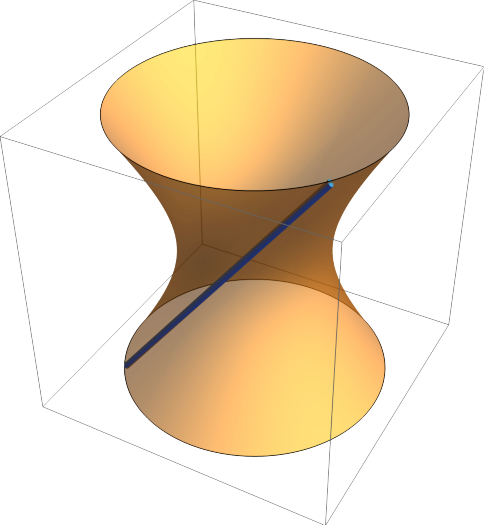
\includegraphics[width=\linewidth]{figures/line-on-hyperboloid.png}}
  \[
    x^{2}+y^{2}-z^{2}-1=(x+z)(x-z)+(y+1)(y-1)\in J.
  \]
\end{Example}

讨论了包含之后, 现在来看交与并. 一族仿射簇的交或并还是仿射簇吗? 如果是, 而且我们恰好知道原来那一族簇的一组定义方程, 能否求出交与并的定义方程? 我们从一个熟悉的例子出发, 探讨这些问题.

\begin{Example}{坐标轴的交与并}\leavevmode\label{ex:coordinate-axes-intersection-and-union}
  考虑仿射簇 $\mathcal{V}(x)\subseteq\mathbb{A}^{2}$ 和 $\mathcal{V}(y)\subseteq\mathbb{A}^{2}$, 它们分别是 $y$ 轴和 $x$ 轴. 两条坐标轴相交于原点. 我们在 Example~\ref{ex:singleton-vanishing-sets} 中看到, 原点由集合 $\{x,y\}$ 同时为零来定义. 因此,
  \begin{equation}\label{eq:coordinate-axes-intersection}
    \mathcal{V}(x)\cap\mathcal{V}(y)=\mathcal{V}(x,y).
  \end{equation}
  另一方面, 它们的并是 Example~\ref{ex:vanishing-set-coordinate-axes} 中的仿射簇, 由多项式 $xy$ 为零来定义. 因此,
  \begin{equation}\label{eq:coordinate-axes-union}
    \mathcal{V}(x)\cup\mathcal{V}(y)=\mathcal{V}(xy).
  \end{equation}
\end{Example}

如果从理想的角度解释等式 \eqref{eq:coordinate-axes-intersection} 和 \eqref{eq:coordinate-axes-union}, 那么等式 \eqref{eq:coordinate-axes-union} 中的理想 $\langle xy\rangle$ 是理想 $\langle x\rangle$ 与 $\langle y\rangle$ 的交. 等式 \eqref{eq:coordinate-axes-intersection} 中的理想 $\langle x,y\rangle$ 并不正好是 $\langle x\rangle$ 与 $\langle y\rangle$ 的并, 因为它们的并不是理想, 而是由这个并集生成的理想 (Exercise~\ref{ex:coordinate-ideals-intersection-and-generated-union}). Example~\ref{ex:coordinate-axes-intersection-and-union} 就这样说明了下面的一般结果.

\begin{Proposition}{零点集的交与并}\leavevmode\label{prop:intersection-and-union-of-vanishing-sets}
  对任意理想 $I,J\subseteq K[x_{1},\ldots,x_{n}]$,
  \[
    \begin{aligned}
      \mathcal{V}(I)\cap\mathcal{V}(J)&=\mathcal{V}(I\cup J),\\
      \mathcal{V}(I)\cup\mathcal{V}(J)&=\mathcal{V}(I\cap J).
    \end{aligned}
  \]
\end{Proposition}

\begin{Proof}
  我们证明第二个等式, 第一个留给 Exercise~\ref{ex:intersection-of-vanishing-sets}.

  ($\subseteq$): 由于 $I\cap J\subseteq I$, Proposition~\ref{prop:operators-reverse-inclusions} 蕴含 $\mathcal{V}(I)\subseteq\mathcal{V}(I\cap J)$. 同理, 有 $\mathcal{V}(J)\subseteq\mathcal{V}(I\cap J)$. 合起来可得
  \[
    \mathcal{V}(I)\cup\mathcal{V}(J)\subseteq\mathcal{V}(I\cap J).
  \]

  ($\supseteq$): 设 $a=(a_{1},\ldots,a_{n})\notin\mathcal{V}(I)\cup\mathcal{V}(J)$. 因为 $a\notin\mathcal{V}(I)$, 所以存在 $f\in I$ 使 $f(a)\ne0$. 类似地, 存在 $g\in J$ 使 $g(a)\ne0$. 因为理想吸收乘法, 乘积 $fg$ 既在 $I$ 中又在 $J$ 中, 所以 $fg\in I\cap J$. 由于
  \[
    (fg)(a)=f(a)g(a)\ne0,
  \]
  可得 $a\notin\mathcal{V}(I\cap J)$, 证明完毕.
\end{Proof}

由于每个仿射簇 $X$ 都是某个理想的零点集, 即理想 $\mathcal{I}(X)$ 的零点集, Proposition~\ref{prop:intersection-and-union-of-vanishing-sets} 蕴含任意两个仿射簇的交与并本身都是仿射簇. 不过, Proposition~\ref{prop:intersection-and-union-of-vanishing-sets} 中的两个等式各有一个不便之处. 在第一个等式中, 问题在于理想的并 $I\cup J$ 一般不是理想 (Exercise~\ref{ex:when-union-of-ideals-is-ideal}). 在第二个等式中, 虽然 $I\cap J$ 是理想, 但在实际运算中可能并不方便. 例如, 即使知道 $I$ 和 $J$ 的生成元, 也不能直接看出怎样求 $I\cap J$ 的生成元.

用下面两种理想的代数运算来重新表述 Proposition~\ref{prop:intersection-and-union-of-vanishing-sets}, 就能解决这两个问题.

\begin{Definition}{理想的和与积}\leavevmode\label{def:sum-and-product-of-ideals}
  设 $I$ 和 $J$ 为环 $R$ 中的理想. $I$ 与 $J$ 的\textbf{和}是理想
  \[
    I+J=\{r+s\mid r\in I,s\in J\},
  \]
  而 $I$ 与 $J$ 的\textbf{积}是理想
  \[
    I\cdot J=\left\{\sum_{i=1}^{m}r_{i}s_{i}\ \middle|\,
      m\in\mathbb{N},r_{i}\in I,s_{i}\in J\right\}.
  \]
\end{Definition}

两个理想的和的定义正如人们所预期的: 把两个理想的元素两两相加所得的集合, 恰好是一个理想. 然而, 积的定义需要额外一步: 由于两两相乘所得的集合对加法不封闭, 要得到一个理想, 就必须把两两乘积的所有有限和都包括进来. 验证两个理想的和与积确实都是理想, 留给 Exercise~\ref{ex:ideal-sum-and-product-properties}; 这道习题还给出了其他一些有用的性质.

处理理想的和与积时, 一个重要之处是: 如果已知 $I$ 和 $J$ 的生成元, 比如 $I=\langle a_{1},\ldots,a_{k}\rangle$ 和 $J=\langle b_{1},\ldots,b_{\ell}\rangle$, 就能直接写出和理想及积理想的生成元 (Exercise~\ref{ex:ideal-sum-and-product-properties}):
\[
  \begin{aligned}
    I+J&=\langle a_{1},\ldots,a_{k},b_{1},\ldots,b_{\ell}\rangle,\\
    I\cdot J&=\langle a_{i}b_{j}\mid i=1,\ldots,k\text{ 且 }j=1,\ldots,\ell\rangle.
  \end{aligned}
\]
例如, 在环 $K[x,y]$ 中, 有
\[
  \begin{aligned}
    \langle x\rangle+\langle y\rangle&=\langle x,y\rangle,\\
    \langle x\rangle\cdot\langle y\rangle&=\langle xy\rangle.
  \end{aligned}
\]
利用和与积, 可以把 Proposition~\ref{prop:intersection-and-union-of-vanishing-sets} 改述如下.

\begin{Proposition}{再论交与并}\leavevmode\label{prop:vanishing-sets-of-ideal-sum-and-product}
  对任意理想 $I,J\subseteq K[x_{1},\ldots,x_{n}]$,
  \[
    \begin{aligned}
      \mathcal{V}(I)\cap\mathcal{V}(J)&=\mathcal{V}(I+J),\\
      \mathcal{V}(I)\cup\mathcal{V}(J)&=\mathcal{V}(I\cdot J).
    \end{aligned}
  \]
\end{Proposition}

\begin{Proof}
  对第一个等式, 只需留意 $I+J$ 是由 $I\cup J$ 生成的理想 (Exercise~\ref{ex:ideal-sum-and-product-properties}), 则 Proposition~\ref{prop:vanishing-sets-of-ideal-sum-and-product} 的第一个等式可由 Proposition~\ref{prop:intersection-and-union-of-vanishing-sets} 的第一个等式得到.

  为证第二个等式, 注意 $I\cdot J$ 包含在 $I$ 和 $J$ 两者之中 (Exercise~\ref{ex:ideal-sum-and-product-properties}). 因此, $\mathcal{V}(I)\cup\mathcal{V}(J)\subseteq\mathcal{V}(I\cdot J)$ 的证明可以原样照搬 Proposition~\ref{prop:intersection-and-union-of-vanishing-sets} 的证明. 类似地, 由于当 $f\in I$ 且 $g\in J$ 时总有 $fg\in I\cdot J$, $\mathcal{V}(I)\cup\mathcal{V}(J)\supseteq\mathcal{V}(I\cdot J)$ 的证明也可原样照用.
\end{Proof}

\begin{Example}{借助理想求交与并}\leavevmode\label{ex:intersection-and-union-via-ideals}
  考虑 $\mathbb{A}^{2}$ 中的仿射簇 $\mathcal{V}(x,y)$ 和 $\mathcal{V}(x-y)$, 它们是原点与过原点的一条直线. 本例用代数方法计算它们的交与并, 验证预期的结果.

  应用 Proposition~\ref{prop:vanishing-sets-of-ideal-sum-and-product} 以及理想的和的生成元描述, 有
  \[
    \mathcal{V}(x,y)\cap\mathcal{V}(x-y)
      =\mathcal{V}(\langle x,y\rangle+\langle x-y\rangle)=\mathcal{V}(x,y,x-y).
  \]
  注意 $\langle x,y,x-y\rangle=\langle x,y\rangle$, 因为 $x-y$ 已在 $x$ 和 $y$ 生成的理想中. 所以上式可写成
  \[
    \mathcal{V}(x,y)\cap\mathcal{V}(x-y)=\mathcal{V}(x,y),
  \]
  它表达了这两个仿射簇的交为原点这一几何事实.

  至于它们的并, Proposition~\ref{prop:vanishing-sets-of-ideal-sum-and-product} 蕴含
  \[
    \mathcal{V}(x,y)\cup\mathcal{V}(x-y)
      =\mathcal{V}(\langle x,y\rangle\cdot\langle x-y\rangle)
      =\mathcal{V}(x(x-y),y(x-y)).
  \]
  元素 $(a,b)\in\mathcal{V}(x(x-y),y(x-y))$ 必须满足方程
  \[
    a(a-b)=0 \qquad\text{和}\qquad b(a-b)=0.
  \]
  第一个方程蕴含 $a=0$ 或 $a=b$. 若 $a=0$, 则第二个方程蕴含 $b^{2}=0$, 所以 $b=0$. 若 $a=b$, 则第二个方程自动满足. 由此可验证
  \[
    \mathcal{V}(x(x-y),y(x-y))=\{(a,b)\in\mathbb{A}^{2}\mid a=b\}.
  \]
  换句话说, 我们用代数方法验证了, 正如预期, 原点与直线 $y=x$ 的并就是这条直线.
\end{Example}

到目前为止, 我们只考虑了两个仿射簇的并与交. 不过细心的读者或许已经发现, 上述一切都可以推广到有限多个仿射簇 $\mathcal{V}(I_{1}),\ldots,\mathcal{V}(I_{k})$ 的并与交. 实际上, 交还可以进一步推广, 允许可数无穷多个仿射簇 $\mathcal{V}(I_{1}),\mathcal{V}(I_{2}),\mathcal{V}(I_{3}),\ldots$, 甚至不可数多个仿射簇.

在记号上, 为了讨论任意一族理想, 我们考虑集合 $\{I_{\alpha}\}_{\alpha\in A}$, 其中 $A$ 是任意集合 (称为指标集), 且对每个 $\alpha\in A$, $I_{\alpha}\subseteq K[x_{1},\ldots,x_{n}]$ 是一个理想. 例如, 如果 $A=\{1,2,3\}$, 这就是一族理想 $\{I_{1},I_{2},I_{3}\}$. 如果 $A=\mathbb{N}$, 这就是可数无穷多个理想 $\{I_{0},I_{1},I_{2},\ldots\}$. 甚至可以取 $A=\mathbb{R}$, 这意味着这一族不仅含理想 $I_{0},I_{1},I_{2},\ldots$, 还含理想 $I_{-1},I_{1/2},I_{\sqrt{2}},I_{\pi}$ 等等.

有了这个记号, 一般结果如下.

\begin{Proposition}{一般的交与并}\leavevmode\label{prop:arbitrary-intersections-and-finite-unions}
  对任意一族理想 $\{I_{\alpha}\}_{\alpha\in A}$, 其中 $I_{\alpha}\subseteq K[x_{1},\ldots,x_{n}]$, 有
  \[
    \bigcap_{\alpha\in A}\mathcal{V}(I_{\alpha})
      =\mathcal{V}\left(\bigcup_{\alpha\in A}I_{\alpha}\right).
  \]
  对任意有限族理想 $\{I_{1},\ldots,I_{k}\}$, 其中 $I_{i}\subseteq K[x_{1},\ldots,x_{n}]$, 有
  \[
    \bigcup_{i=1}^{k}\mathcal{V}(I_{i})
      =\mathcal{V}\left(\bigcap_{i=1}^{k}I_{i}\right).
  \]
\end{Proposition}

\begin{Proof}
  \BookPairedNote
    {证明仿照 Proposition~\ref{prop:intersection-and-union-of-vanishing-sets} 的证明. 第二个等式要求有限性, 是因为 Proposition~\ref{prop:intersection-and-union-of-vanishing-sets} 证明中出现的乘积 $fg$, 在这里要换成从每个 $I_{i}$ 中各取一个 $f_{i}$ 所成的乘积, 而无穷多个多项式的乘积并不是多项式.}
    {Proposition~\ref{prop:arbitrary-intersections-and-finite-unions} 也可以用理想的和与积来表述, 但定义理想的无穷和时需要略加小心.}
\end{Proof}

仿射簇的并要成为仿射簇, 有限性是不可少的. 例如, $\mathbb{Z}\subseteq\mathbb{C}=\mathbb{A}^{1}_{\mathbb{C}}$ 是其中各点的无限并, 每个点都是仿射簇. 但我们知道 $\mathbb{Z}\subseteq\mathbb{A}^{1}_{\mathbb{C}}$ 不是仿射簇, 因为它既不是有限集, 也不是整个 $\mathbb{A}^{1}_{\mathbb{C}}$.

Proposition~\ref{prop:arbitrary-intersections-and-finite-unions} 蕴含仿射簇的任意交与有限并都是仿射簇. 熟悉拓扑学的读者也许会认出这些条件: 连同 $\varnothing$ 和 $\mathbb{A}^{n}$ 都是仿射簇这一事实, 它们构成一个拓扑的闭集的定义条件, 因而闭集的补集构成开集. $\mathbb{A}^{n}$ 上的这一拓扑称为 \textbf{Zariski 拓扑}, 得名于 Oscar Zariski (1899--1986). 他受过经典意大利学派方法的训练, 将这种方法奠定在更严格的代数基础之上, 为现代代数几何作出了奠基性贡献.

虽然本书并不假定读者熟悉拓扑学, 但 Zariski 开集与 Zariski 闭集的术语遍见于代数几何, 所以我们在此给出定义, 以供后文参考.

\begin{Definition}{$\mathbb{A}^{n}$ 上的 Zariski 拓扑}\leavevmode\label{def:zariski-topology}
  若子集 $X\subseteq\mathbb{A}^{n}$ 是仿射簇, 则称 $X$ 是 \textbf{Zariski 闭的}.

  若子集 $U\subseteq\mathbb{A}^{n}$ 的补集 $\mathbb{A}^{n}\setminus U$ 是仿射簇, 则称 $U$ 是 \textbf{Zariski 开的}.
\end{Definition}

\BookPairedNote
  {修饰语\textquotedbl{}Zariski\textquotedbl{}将这个拓扑与 $\mathbb{A}^{n}_{K}$ 上其他自然的拓扑区分开来, 例如 $K=\mathbb{R}$ 或 $\mathbb{C}$ 时的欧氏拓扑.}
  {有拓扑学背景且对此感兴趣的读者, 可参看 Exercise~\ref{ex:compare-zariski-and-euclidean-topologies}, 探索 Zariski 拓扑的一些基本性质及其与欧氏拓扑的比较.}

\BookExerciseHeading
\begin{BookExercises}
  \item\label{ex:vanishing-sets-reverse-inclusion} 设 $S,T\subseteq K[x_{1},\ldots,x_{n}]$ 为子集.
    \begin{enumerate}[label=(\alph*),ref=(\alph*)]
      \item\label{item:vanishing-sets-inclusion-proof} 证明 $S\subseteq T$ 蕴含 $\mathcal{V}(S)\supseteq\mathcal{V}(T)$.
      \item 举例证明 \ref{item:vanishing-sets-inclusion-proof} 的逆命题可能不成立.
    \end{enumerate}
  \item\label{ex:vanishing-ideals-reverse-inclusion} 设 $X,Y\subseteq\mathbb{A}^{n}$ 为子集.
    \begin{enumerate}[label=(\alph*),ref=(\alph*)]
      \item\label{item:vanishing-ideals-inclusion-proof} 证明 $X\subseteq Y$ 蕴含 $\mathcal{I}(X)\supseteq\mathcal{I}(Y)$.
      \item 举例证明 \ref{item:vanishing-ideals-inclusion-proof} 的逆命题可能不成立.
    \end{enumerate}
  \item\label{ex:coordinate-ideals-intersection-and-generated-union} 本题涉及理想 $\langle x\rangle\subseteq K[x,y]$ 与 $\langle y\rangle\subseteq K[x,y]$.
    \begin{enumerate}[label=(\alph*)]
      \item 证明 $\langle x\rangle\cap\langle y\rangle=\langle xy\rangle$.
      \item 证明 $\langle x\rangle\cup\langle y\rangle=\langle x,y\rangle$.
    \end{enumerate}
  \item\label{ex:intersection-of-vanishing-sets} 证明对任意理想 $I,J\subseteq K[x_{1},\ldots,x_{n}]$, 都有
    \[
      \mathcal{V}(I)\cap\mathcal{V}(J)=\mathcal{V}(I\cup J),
    \]
    以补全 Proposition~\ref{prop:intersection-and-union-of-vanishing-sets} 的证明.
  \item\label{ex:when-union-of-ideals-is-ideal} 证明环中两个理想的并是理想, 当且仅当其中一个理想包含在另一个中.
  \item\label{ex:pairwise-products-need-not-be-ideal} 设 $I,J$ 是环 $R$ 的理想. 举例证明 $\{ab\mid a\in I,b\in J\}$ 不一定是 $R$ 的理想.
  \item\label{ex:ideal-sum-and-product-properties} 设 $I$ 和 $J$ 为环 $R$ 中的理想.
    \begin{enumerate}[label=(\alph*)]
      \item 证明 $I+J$ 和 $I\cdot J$ 都是理想.
      \item 假设 $I=\langle a_{1},\ldots,a_{k}\rangle$ 且 $J=\langle b_{1},\ldots,b_{\ell}\rangle$. 证明
        \[
          I+J=\langle a_{1},\ldots,a_{k},b_{1},\ldots,b_{\ell}\rangle
        \]
        以及
        \[
          I\cdot J=\langle a_{i}b_{j}\mid i=1,\ldots,k,\ j=1,\ldots,\ell\rangle.
        \]
      \item 证明 $I+J$ 是由 $I\cup J$ 生成的理想.
      \item 证明 $I\cdot J\subseteq I\cap J$.
    \end{enumerate}
  \item\label{ex:nonempty-zariski-opens-intersect} 假设 $K$ 是无限域. 证明 $\mathbb{A}^{n}_{K}$ 中任意两个非空 Zariski 开集的交非空. (对有一定拓扑学背景的学生来说, 这意味着 $\mathbb{A}^{n}_{K}$ 上的 Zariski 拓扑不是 Hausdorff 的.)
  \item\label{ex:compare-zariski-and-euclidean-topologies} (供有一定拓扑学背景的学生.) 比较 $\mathbb{A}^{n}_{\mathbb{R}}=\mathbb{R}^{n}$ 上的 Zariski 拓扑和欧氏拓扑. 其中一个拓扑是否比另一个粗?
\end{BookExercises}

\section{有限生成}\label{sec:finite-generation}

无论 $S$ 是有限集还是无限集, 零点集 $\mathcal{V}(S)$ 都有意义, 但我们往往可以用有限集来替换无限集, 而不影响相应的零点集. 例如, 理想 $\langle y-x^{2}\rangle\subseteq K[x,y]$ 含有无穷多个多项式, 但 $\mathcal{V}(\langle y-x^{2}\rangle)$ 等于 $\mathcal{V}(y-x^{2})$, 即仅由一个多项式给出的零点集.

于是一个自然的问题是: 是否每个仿射簇都等于某个有限集 $S$ 的 $\mathcal{V}(S)$? 答案是肯定的, 给出这一事实的代数证明是本节的主要目标. 先介绍一点代数术语.

\begin{Definition}{有限生成理想}\leavevmode\label{def:finitely-generated-ideal}
  若 $I=\langle r_{1},\ldots,r_{k}\rangle$, 其中 $r_{1},\ldots,r_{k}\in R$ 是有限多个元素, 则称环 $R$ 的理想 $I$ 是\textbf{有限生成的}.
\end{Definition}

例如, 理想 $\langle y-x^{2}\rangle\subseteq K[x,y]$ 是有限生成的, 理想 $\langle x,y\rangle\subseteq K[x,y]$ 也是. 事实上, 要找一个不是有限生成的理想的例子, 必须考察一个不太熟悉的环.

\begin{Example}{一个不是有限生成的理想}\leavevmode\label{ex:infinitely-generated-variable-ideal}
  考虑无穷元多项式环 $K[x_{1},x_{2},x_{3},\ldots]$. 具体来说, $K[x_{1},x_{2},x_{3},\ldots]$ 中的单项式是形如
  \[
    x^{\alpha}=x_{1}^{\alpha_{1}}x_{2}^{\alpha_{2}}x_{3}^{\alpha_{3}}\cdots,
  \]
  的表达式, 其中 $\alpha=(\alpha_{1},\alpha_{2},\alpha_{3},\ldots)$ 为满足下列条件的指数向量:
  \begin{enumerate}[label=(\roman*),ref=(\roman*)]
    \item\label{item:infinite-variable-nonnegative-exponents} 对所有 $i$, 都有 $\alpha_{i}\in\mathbb{N}$;
    \item\label{item:infinite-variable-finite-support} 除有限多个 $i$ 外, 都有 $\alpha_{i}=0$.
  \end{enumerate}
  $R$ 的元素是单项式的有限 $K$-线性组合:
  \[
    f=\sum_{\alpha}a_{\alpha}x^{\alpha},
  \]
  其中求和遍及满足 \ref{item:infinite-variable-nonnegative-exponents} 和 \ref{item:infinite-variable-finite-support} 的所有指数向量 $\alpha$, 系数 $a_{\alpha}$ 是 $K$ 中的元素, 且除有限多个 $\alpha$ 外, 都有 $a_{\alpha}=0$.

  在 $K[x_{1},x_{2},x_{3},\ldots]$ 中, 由所有变量生成的理想
  \[
    I=\langle x_{1},x_{2},x_{3},\ldots\rangle,
  \]
  不是有限生成的, 读者不妨自行验证 (Exercise~\ref{ex:infinite-variable-ideal-not-finitely-generated}).
\end{Example}

尽管有上面的例子, 我们熟悉的许多环都具有这样的性质: 它们的所有理想都是有限生成的. 为纪念 Emmy Noether (1882--1935), 这类环有一个专门的名称. 除了在抽象代数上的开创性工作以外, Noether 还发现了对称性与守恒定律之间的联系, 指引了现代物理学的发展.

\begin{Definition}{Noether 环}\leavevmode\label{def:noetherian-ring}
  若一个环的所有理想都是有限生成的, 则称它是 \textbf{Noether 环}.
\end{Definition}

本节的主要目标是证明 $K[x_{1},\ldots,x_{n}]$ 是 Noether 环. 首先来讨论几个我们已经知道是 Noether 环的熟悉例子.

\begin{Example}{域是 Noether 环}\leavevmode\label{ex:fields-are-noetherian}
  若 $K$ 是任意一个域, 则 $K$ 仅有的理想是 $\{0\}$ 和 $K$. 两者都是有限生成的, 因为 $\{0\}=\langle0\rangle$ 且 $K=\langle1\rangle$. 因此, $K$ 是 Noether 环.
\end{Example}

\begin{Example}{PID 是 Noether 环}\leavevmode\label{ex:principal-ideal-domains-are-noetherian}
  根据定义, 主理想整环中的每个理想都由单个元素生成, 因而都是有限生成的. 所以 $\mathbb{Z}$ 和 $K[x]$ 都是 Noether 环的例子.
\end{Example}

还可以用相互嵌套的理想序列来刻画 Noether 环. 尽管第二种刻画叙述起来没有那么简单, 但正如下面所见, 它在实际运用中很有用.

\begin{Proposition}{升链条件}\leavevmode\label{prop:ascending-chain-condition}
  环 $R$ 是 Noether 环, 当且仅当给定 $R$ 的任意理想 $I_{1},I_{2},I_{3},\ldots$ 满足
  \[
    I_{1}\subseteq I_{2}\subseteq I_{3}\subseteq\cdots,
  \]
  就存在正整数 $k$, 使得对所有 $d\geq k$ 都有 $I_{d}=I_{k}$.
\end{Proposition}

换句话说, Proposition~\ref{prop:ascending-chain-condition} 表明 Noether 环由\textbf{升链条件}刻画: 任何理想的升链最终都必定稳定. 环 $R=K[x_{1},x_{2},x_{3},\ldots]$ 不是 Noether 环, 并不满足升链条件. 例如, 理想链
\[
  \langle x_{1}\rangle\subsetneq\langle x_{1},x_{2}\rangle
  \subsetneq\langle x_{1},x_{2},x_{3}\rangle\subsetneq\cdots
\]
每一步都严格增加.

\begin{Proof}\unskip\textbf{ of Proposition~\ref{prop:ascending-chain-condition}}\quad
  我们证明两个方向.

  ($\Rightarrow$) 假设 $R$ 是 Noether 环, 且
  \[
    I_{1}\subseteq I_{2}\subseteq I_{3}\subseteq\cdots
  \]
  是 $R$ 中的一条理想升链. 考虑这些相互嵌套的理想的并
  \[
    I=\bigcup_{k=1}^{\infty}I_{k},
  \]
  根据 Exercise~\ref{ex:ascending-ideal-union}, 这是 $R$ 的一个理想. 由于 $R$ 是 Noether 环, 对某些 $a_{1},\ldots,a_{r}\in R$, 有 $I=\langle a_{1},\ldots,a_{r}\rangle$. 每个 $a_{i}$ 都在各 $I_{k}$ 的并中, 所以它必属于其中一个, 设 $a_{i}\in I_{k_{i}}$. 由于这些理想相互嵌套, 对所有 $d\geq k_{i}$ 都有 $a_{i}\in I_{d}$. 特别地, 令 $k=\max\{k_{1},\ldots,k_{r}\}$, 则对所有 $d\geq k$ 都有 $\{a_{1},\ldots,a_{r}\}\subseteq I_{d}$, 从而对于所有 $d\geq k$ 都有 $I=\langle a_{1},\ldots,a_{r}\rangle\subseteq I_{d}$. 另一方面, 由于 $I$ 是各 $I_{k}$ 的并, 还有 $I\supseteq I_{d}$. 由此得对所有 $d\geq k$, 都有 $I=I_{d}$, 验证了升链条件.

  ($\Leftarrow$) 我们证明这个方向的逆否命题. 假设 $R$ 不是 Noether 环, 选取 $R$ 的一个不是有限生成的理想 $I$. 任取一个元素 $a_{1}\in I$, 定义 $I_{1}=\langle a_{1}\rangle$. 那么 $I_{1}\subseteq I$, 但因为 $I$ 不是有限生成的, 这个包含关系必是严格的. 因而可以选取元素 $a_{2}\in I\setminus I_{1}$, 定义 $I_{2}=\langle a_{1},a_{2}\rangle$. 现在有
  \[
    I_{1}\subsetneq I_{2}\subsetneq I;
  \]
  第一个包含关系是严格的, 因为 $a_{2}\notin I_{1}$; 第二个包含关系也是严格的, 因为 $I$ 不是有限生成的. 选取 $a_{n+1}\in I\setminus\langle a_{1},\ldots,a_{n}\rangle$ 并定义 $I_{n+1}=\langle a_{1},\ldots,a_{n+1}\rangle$, 就能将这个过程无限继续下去. 这个过程递归地产生一条永不稳定的理想升链, 所以升链条件不成立.
\end{Proof}

\BookPairedNote
  {有了用升链来刻画 Noether 性的结果, 现在就能证明多项式环 $K[x_{1},\ldots,x_{n}]$ 是 Noether 环. 证明用归纳法, 每次添加一个变量. 归纳步骤由下面这个关键的代数结果给出.}
  {\textquotedbl{}基\textquotedbl{}这个词多少有些过时: 在 Hilbert 的时代, 理想的一组生成元称为一组基. 这个术语在某种程度上沿用至今, 例如还出现在\textquotedbl{}Gröbner 基\textquotedbl{}中, 但已相对少见.}
\noindent 这一结果称为 Hilbert 基定理, 得名于成果颇丰的数学家 David Hilbert (1862--1943). 他于 1890 年在研究不变量理论时首次证明了这个结果.

\begin{Theorem}{Hilbert 基定理}\leavevmode\label{thm:hilbert-basis-theorem}
  如果 $R$ 是 Noether 环, 那么 $R[x]$ 是 Noether 环.
\end{Theorem}

\begin{Proof}
  假设 $R$ 是 Noether 环, 并反设 $R[x]$ 不是 Noether 环. 令 $I\subseteq R[x]$ 为一个不是有限生成的理想. 按如下递归过程定义 $R[x]$ 中的一个无穷多项式序列:
  \begin{enumerate}[label=\arabic*.]
    \item 选取 $f_{1}\in I$ 为一个次数最小的非零多项式.
    \item 选定 $f_{1},\ldots,f_{j}\in I$ 后, 选取 $f_{j+1}\in I\setminus\langle f_{1},\ldots,f_{j}\rangle$ 为一个次数最小的非零多项式.
  \end{enumerate}
  不可能有 $\deg(f_{j})>\deg(f_{j+1})$, 否则与 $f_{j}$ 在 $I\setminus\langle f_{1},\ldots,f_{j-1}\rangle$ 中次数最小的选法矛盾. 因此, 序列 $(f_{1},f_{2},f_{3},\ldots)$ 中多项式的次数是非递减的.

  对每个 $j$, 令 $a_{j}$ 为 $f_{j}$ 的首项系数, 并考虑 $R$ 中的如下理想升链:
  \[
    \langle a_{1}\rangle\subseteq\langle a_{1},a_{2}\rangle
    \subseteq\langle a_{1},a_{2},a_{3}\rangle\subseteq\cdots.
  \]
  由于 $R$ 是 Noether 环, 这条链最终一定稳定. 假设它在第 $k$ 步稳定. 则 $a_{k+1}\in\langle a_{1},\ldots,a_{k}\rangle$. 选取元素 $r_{1},\ldots,r_{k}\in R$, 使得
  \[
    a_{k+1}=r_{1}a_{1}+\cdots+r_{k}a_{k}.
  \]
  利用对所有 $i\leq k$ 都有 $\deg(f_{i})\leq\deg(f_{k+1})$ 这一事实, 定义多项式
  \[
    g=x^{\deg(f_{k+1})-\deg(f_{1})}r_{1}f_{1}
      +\cdots+x^{\deg(f_{k+1})-\deg(f_{k})}r_{k}f_{k}\in R[x].
  \]
  按照这一构造, $g$ 与 $f_{k+1}$ 有相同的首项, 从而
  \[
    \deg(f_{k+1}-g)<\deg(f_{k+1}).
  \]
  由于 $f_{k+1}$ 和 $g$ 都是 $I$ 的元素, 可知 $f_{k+1}-g\in I$. 然而, $g$ 是 $\langle f_{1},\ldots,f_{k}\rangle$ 的元素而 $f_{k+1}$ 不是, 故 $f_{k+1}-g$ 不可能属于 $\langle f_{1},\ldots,f_{k}\rangle$. 因此 $f_{k+1}-g\in I\setminus\langle f_{1},\ldots,f_{k}\rangle$, 且 $\deg(f_{k+1}-g)<\deg(f_{k+1})$, 这与选择 $f_{k+1}$ 时的次数最小性矛盾.
\end{Proof}

这样就得出了多项式环的以下基本性质.

\begin{Corollary}{{\textmd{$K[x_{1},\ldots,x_{n}]$} 是 Noether 环}}\leavevmode\label{cor:polynomial-rings-are-noetherian}
  \strut\par\nopagebreak[4]\noindent
  对任意域 $K$, 多项式环 $K[x_{1},\ldots,x_{n}]$ 是 Noether 环.
\end{Corollary}

\begin{Proof}
  对 $n$ 作归纳.

  (归纳起点) 如 Example~\ref{ex:fields-are-noetherian} 所述, 任意域 $K$ 都是 Noether 环, 这就证明了 $n=0$ 的情形.

  (归纳步骤) 假设 $K[x_{1},\ldots,x_{n-1}]$ 是 Noether 环. 利用典范同构
  \[
    K[x_{1},\ldots,x_{n}]=K[x_{1},\ldots,x_{n-1}][x_{n}]
  \]
  并对 $R=K[x_{1},\ldots,x_{n-1}]$ 应用 Hilbert 基定理, 可知 $K[x_{1},\ldots,x_{n}]$ 是 Noether 环.
\end{Proof}

$K[x_{1},\ldots,x_{n}]$ 是 Noether 环的几何含义是: 每个仿射簇都可以定义为有限多个多项式的零点集. 实际上, 还有一个稍强的结论, 如下一个结果所述.

\begin{Corollary}{仿射簇是有限生成的}\leavevmode\label{cor:affine-varieties-finitely-generated}
  对任意子集 $S\subseteq K[x_{1},\ldots,x_{n}]$, 都存在有限子集 $T\subseteq S$, 使得
  \[
    \mathcal{V}(S)=\mathcal{V}(T).
  \]
\end{Corollary}

\begin{Proof}
  \BookPairedNote
    {令 $S\subseteq K[x_{1},\ldots,x_{n}]$ 为一个 (可能是无限的) 集合. 根据 Corollary~\ref{cor:polynomial-rings-are-noetherian}, 存在 $f_{1},\ldots,f_{k}\in K[x_{1},\ldots,x_{n}]$, 使得
    \[
      \langle S\rangle=\langle f_{1},\ldots,f_{k}\rangle.
    \]}
    {这个结果比仅仅说 $\mathcal{V}(S)$ 可以用一个有限多项式集合来定义更强. 它还断言这个有限集可以选为 $S$ 的子集.}
  \noindent 多项式 $f_{1},\ldots,f_{k}$ 本身未必都属于集合 $S$, 但由 $\langle S\rangle$ 的定义, 我们可以把每个 $f_{i}$ 写成 $S$ 中元素的线性组合:
  \begin{equation}\label{eq:finite-generators-in-span-of-original-set}
    f_{i}=\sum_{j=1}^{\ell_{i}}g_{i,j}h_{i,j}
  \end{equation}
  其中 $g_{i,j}\in K[x_{1},\ldots,x_{n}]$, $h_{i,j}\in S$. 定义有限子集
  \[
    T=\{h_{i,j}\mid1\leq i\leq k,\ 1\leq j\leq\ell_{i}\}\subseteq S.
  \]
  等式 \eqref{eq:finite-generators-in-span-of-original-set} 蕴含对所有 $i$, 都有 $f_{i}\in\langle T\rangle$, 所以 $\langle S\rangle=\langle f_{1},\ldots,f_{k}\rangle\subseteq\langle T\rangle$. 反过来, 由于 $T\subseteq S$, 得到 $\langle T\rangle\subseteq\langle S\rangle$. 因此 $\langle S\rangle=\langle T\rangle$, 从而
  \[
    \mathcal{V}(S)=\mathcal{V}(\langle S\rangle)=\mathcal{V}(\langle T\rangle)=\mathcal{V}(T).
  \]
\end{Proof}

\BookExerciseHeading
\begin{BookExercises}
  \item\label{ex:infinite-variable-ideal-not-finitely-generated} 证明 $\langle x_{1},x_{2},x_{3},\ldots\rangle\subseteq K[x_{1},x_{2},x_{3},\ldots]$ 不是有限生成的.
  \item\label{ex:ascending-chain-of-integer-ideals} 因为 $\mathbb{Z}$ 是主理想整环 (因而是 Noether 环), Proposition~\ref{prop:ascending-chain-condition} 蕴含 $\mathbb{Z}$ 中任何理想升链 $I_{1}\subseteq I_{2}\subseteq I_{3}\subseteq\cdots$ 必定稳定. 具体解释这个现象: 即把各 $I_{i}$ 写成 $I_{i}=\langle a_{i}\rangle$, 其中 $a_{i}$ 为某个整数, 那么 $a_{i}$ 与 $a_{i+1}$ 之间有什么关系? 为什么一定存在 $k\in\mathbb{N}$, 使 $a_{k}=a_{k+1}=a_{k+2}=\cdots$?
  \item\label{ex:quotient-of-noetherian-ring} 设 $R$ 是 Noether 环, $I\subseteq R$ 是理想. 证明 $R/I$ 是 Noether 环.
  \item\label{ex:noetherian-ring-as-factorization-domain} 证明每个 Noether 环都是分解整环.
  \item\label{ex:subring-need-not-be-noetherian} 本题说明 Noether 环的子环不一定是 Noether 环. 记 $K[yz,yz^{2},yz^{3},\ldots]$ 为环同态
    \[
      \begin{aligned}
        \phi:K[x_{1},x_{2},x_{3},\ldots]&\to K[y,z]\\
        f(x_{1},x_{2},x_{3},\ldots)&\mapsto f(yz,yz^{2},yz^{3},\ldots).
      \end{aligned}
    \]
    的像. 证明 $K[yz,yz^{2},yz^{3},\ldots]$ 是 $K[y,z]$ 的一个不是 Noether 环的子环.
  \item\label{ex:noetherian-surjective-endomorphism} 设 $R$ 是 Noether 环, 且 $\phi:R\to R$ 是环同态. 证明 $\phi$ 是同构当且仅当 $\phi$ 是满射. (提示: 考察理想 $I_{1}=\ker(\phi)$, $I_{2}=\ker(\phi\circ\phi)$, $I_{3}=\ker(\phi\circ\phi\circ\phi)$ 等.)
  \item\label{ex:zariski-topology-is-compact} 假设
    \[
      \mathbb{A}^{n}=\bigcup_{\alpha\in A}U_{\alpha}
    \]
    其中每个 $U_{\alpha}\subseteq\mathbb{A}^{n}$ 都是 Zariski 开集. 证明存在有限子集 $B\subseteq A$, 使得
    \[
      \mathbb{A}^{n}=\bigcup_{\alpha\in B}U_{\alpha}.
    \]
    (对有一定拓扑学背景的学生来说, 这是说 $\mathbb{A}^{n}$ 上的 Zariski 拓扑是紧的.)
\end{BookExercises}

\section{不可约仿射簇}\label{sec:irreducible-affine-varieties}

现在来到本章的核心, 也是代数几何中的一个中心概念: 不可约性. 为了引出这一概念, 考虑仿射簇
\[
  X_{1}=\mathcal{V}(y-x^{2}),\quad X_{2}=\mathcal{V}(y-2),
  \quad\text{以及}\quad X_{3}=\mathcal{V}(x-1,y-3).
\]
\BookPairedFigure
  {$\mathbb{R}$ 上的仿射簇 $X=X_{1}\cup X_{2}\cup X_{3}$ 画在\hyperref[fig:three-irreducible-pieces]{右边}. 设想只给你看这幅图, 却不告诉你 $X$ 是三个仿射簇的并. 你很可能仍能从图上看出 $X$ 是这样的并, 仔细看图甚至可能确定这三个簇.}
  {\phantomsection\label{fig:three-irreducible-pieces}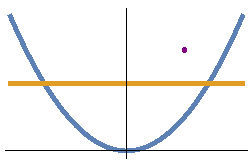
\includegraphics[width=\linewidth]{figures/three-irreducible-pieces.pdf}}
\noindent 这些簇是 $X$ 的基本组成部分, 即它的不可约分支.

如上所述, 把仿射簇分解成各个组成部分, 就是把它写成有限多个较小仿射簇的并. 因此, 基本组成部分正是那些不能写成两个较小仿射簇之并的仿射簇. 下面的定义把这一概念精确化.

\begin{Definition}{可约与不可约仿射簇}\leavevmode\label{def:reducible-and-irreducible-affine-varieties}
  若对某些仿射簇 $X_{1},X_{2}\subsetneq X$, 有 $X=X_{1}\cup X_{2}$, 则称仿射簇 $X\subseteq\mathbb{A}^{n}$ 是\textbf{可约的}. 若 $X$ 既非空也不是可约的, 则称它是\textbf{不可约的}.
\end{Definition}

\begin{Example}{}\leavevmode\label{ex:two-lines-reducible-variety}
  仿射簇 $X=\mathcal{V}(x^{2}-y^{2})\subseteq\mathbb{A}^{2}_{\mathbb{C}}$ 是可约的. 为见此点, 注意
  \[
    X=\mathcal{V}((x+y)(x-y))=\mathcal{V}(x+y)\cup\mathcal{V}(x-y).
  \]
  \BookPairedFigure
    {因此, 两个仿射簇
    \[
      X_{1}=\mathcal{V}(x+y)\subsetneq X
    \]
    与
    \[
      X_{2}=\mathcal{V}(x-y)\subsetneq X
    \]
    满足 $X=X_{1}\cup X_{2}$.}
    {\phantomsection\label{fig:two-crossing-lines}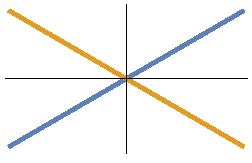
\includegraphics[width=\linewidth]{figures/two-crossing-lines.pdf}}
  \noindent 限制到实数时, 由\hyperref[fig:two-crossing-lines]{上图}可见, $X_{1}$ 和 $X_{2}$ 是构成 $X$ 的两条直线. 实际上, 如下一节将看到的, 簇 $X_{1}$ 和 $X_{2}$ 是 $X$ 的唯一两个不可约分支.
\end{Example}

\begin{Example}{}\leavevmode\label{ex:parabola-geometrically-irreducible}
  相比之下, 抛物线 $X=\mathcal{V}(y-x^{2})\subseteq\mathbb{A}^{2}$ 是不可约的. 从几何上看, 这个断言应当是可信的: 与 Example~\ref{ex:two-lines-reducible-variety} 中的仿射簇不同, 抛物线只由一\textquotedbl{}块\textquotedbl{}组成. 虽然这一直觉还不是证明, 但 $X$ 的不可约性可由下面的 Proposition~\ref{prop:irreducible-iff-vanishing-ideal-prime} 得出.
\end{Example}

如上面的例子所示, 证明仿射簇 $X$ 可约很直接: 找到一对仿射簇 $X_{1}\subsetneq X$ 和 $X_{2}\subsetneq X$, 使两者的并为 $X$. 怎样证明仿射簇不可约则没有那么明显. 下面用代数方法刻画不可约性, 提供一个关键工具.

\begin{Proposition}{不可约性的代数刻画}\leavevmode\label{prop:irreducible-iff-vanishing-ideal-prime}
  仿射簇 $X\subseteq\mathbb{A}^{n}$ 是不可约的, 当且仅当 $\mathcal{I}(X)$ 是素理想.
\end{Proposition}

\begin{Proof}
  我们分别证明两个方向的逆否命题.

  ($\Leftarrow$) 假设 $X$ 可约, 选取仿射簇 $X_{1},X_{2}\subsetneq X$, 使得
  \[
    X=X_{1}\cup X_{2}.
  \]
  因为 $X_{1}\subsetneq X$, 由 Proposition~\ref{prop:operators-reverse-inclusions} 得 $\mathcal{I}(X_{1})\supsetneq\mathcal{I}(X)$. 因此, 存在 $f\in\mathcal{I}(X_{1})$ 使 $f\notin\mathcal{I}(X)$. 类似地, 存在 $g\in\mathcal{I}(X_{2})$ 使 $g\notin\mathcal{I}(X)$. 对任意 $a\in X$, 或者有 $a\in X_{1}$ (因而 $f(a)=0$), 或者有 $a\in X_{2}$ (因而 $g(a)=0$). 所以 $(fg)(a)=f(a)g(a)=0$, 从而 $fg\in\mathcal{I}(X)$. 这样就证明了存在一对元素 $f,g\in K[x_{1},\ldots,x_{n}]$, 满足
  \begin{equation}\label{eq:two-factors-outside-vanishing-ideal}
    f\notin\mathcal{I}(X),\quad g\notin\mathcal{I}(X),\quad\text{且}\quad fg\in\mathcal{I}(X),
  \end{equation}
  这证明 $\mathcal{I}(X)$ 不是素理想.

  ($\Rightarrow$) 假设 $\mathcal{I}(X)$ 不是素理想, 选取满足 \eqref{eq:two-factors-outside-vanishing-ideal} 中条件的 $f,g\in K[x_{1},\ldots,x_{n}]$. 定义
  \[
    X_{1}=\mathcal{V}(f)\cap X \qquad\text{且}\qquad X_{2}=\mathcal{V}(g)\cap X.
  \]
  Proposition~\ref{prop:intersection-and-union-of-vanishing-sets} 蕴含 $X_{1}$ 与 $X_{2}$ 都是仿射簇, 且都包含在 $X$ 中. 此外, 这两个包含关系都必定是严格的. 例如, 若 $X=X_{1}$, 则 $X=\mathcal{V}(f)\cap X$, 这意味着 $X\subseteq\mathcal{V}(f)$. 若果真如此, 那么对所有 $a\in X$, 都有 $f(a)=0$, 即 $f\in\mathcal{I}(X)$, 与假设矛盾.

  根据构造, 有 $X_{1}\cup X_{2}\subseteq X$, 但反向的包含关系也成立. 为见此点, 取 $a\in X$. 由 $fg\in\mathcal{I}(X)$ 可知 $(fg)(a)=f(a)g(a)=0$. 从而 $f(a)=0$ 或 $g(a)=0$, 因此 $a\in\mathcal{V}(f)$ 或 $a\in\mathcal{V}(g)$. 由于已经假设 $a\in X$, 可知 $a\in\mathcal{V}(f)\cap X=X_{1}$ 或 $a\in\mathcal{V}(g)\cap X=X_{2}$, 所以 $a\in X_{1}\cup X_{2}$. 我们由此找到了两个仿射簇 $X_{1},X_{2}\subsetneq X$, 使得 $X=X_{1}\cup X_{2}$, 因而 $X$ 可约.
\end{Proof}

\begin{Example}{抛物线不可约}\leavevmode\label{ex:parabola-is-irreducible}
  考虑仿射簇 $X=\mathcal{V}(y-x^{2})\subseteq\mathbb{A}^{2}$. 在 Example~\ref{ex:vanishing-ideal-of-parabola} 中, 已求得其消没理想为 $\mathcal{I}(X)=\langle y-x^{2}\rangle$. 因为 $y-x^{2}$ 不可约, $\mathcal{I}(X)$ 是素理想 (Proposition~\ref{prop:irreducible-polynomial-characterization}), 这就证明了 $X$ 不可约.
\end{Example}

仿射簇常用定义方程来描述, 或者等价地, 用理想 $I=\langle f_{1},\ldots,f_{k}\rangle$ 来描述. 然而, 这个定义理想不一定等于消没理想. 这就提出一个问题: 给定理想 $I$, 是否不必知道消没理想, 就能判定 $\mathcal{V}(I)$ 是否不可约? 零点定理给出下面这个有用的答案.

\begin{Proposition}{$\mathcal{V}(I)$ 的不可约性}\leavevmode\label{prop:vanishing-set-of-prime-ideal-is-irreducible}
  如果 $I\subseteq K[x_{1},\ldots,x_{n}]$ 是素理想, 则 $\mathcal{V}(I)$ 不可约. 特别地, 如果 $f\in K[x_{1},\ldots,x_{n}]$ 是不可约多项式, 则 $\mathcal{V}(f)$ 不可约.
\end{Proposition}

\begin{Proof}
  假设 $I$ 是素理想. 那么根据 Proposition~\ref{prop:prime-ideals-are-radical}, $I$ 是根理想. 于是由零点定理,
  \[
    \mathcal{I}(\mathcal{V}(I))=\sqrt{I}=I.
  \]
  因为 $\mathcal{I}(\mathcal{V}(I))$ 是素理想, 由 Proposition~\ref{prop:irreducible-iff-vanishing-ideal-prime} 可知 $\mathcal{V}(I)$ 不可约.

  为证第二个断言, 假设 $f$ 是不可约多项式. 则由 Proposition~\ref{prop:irreducible-polynomial-characterization} 可知 $\langle f\rangle$ 是素理想. 因此, 命题的第一个断言蕴含 $\mathcal{V}(f)=\mathcal{V}(\langle f\rangle)$ 不可约.
\end{Proof}

需要指出, 当 $K$ 不是代数闭域时, Proposition~\ref{prop:vanishing-set-of-prime-ideal-is-irreducible} 不成立. 例如, $x^{2}+1\in\mathbb{R}[x]$ 不可约, 但
\[
  \mathcal{V}(x^{2}+1)=\varnothing\in\mathbb{A}^{1}_{\mathbb{R}},
\]
而根据定义, 空集不是不可约的. 若要看 $\mathbb{R}$ 上定义非空可约簇的不可约多项式的例子, 见 Exercise~\ref{ex:real-irreducible-polynomial-with-reducible-variety}.

不过, 正如前面所说, 利用我们在 $\mathbb{R}$ 上的直觉, 常常有助于了解更一般的簇. 例如, 从直观上应该不难看出抛物线在 $\mathbb{R}$ 上不可约, 因为它只由一\textquotedbl{}块\textquotedbl{}组成. 这一直觉也适用于更一般的域: 在任意无限域 $K$ 上, 簇 $\mathcal{V}(y-x^{2})$ 都不可约. 然而, 在 $\mathbb{R}$ 上采用这种推理时应当谨慎, 如下面的例子所示.

\begin{Example}{双曲线不可约}\leavevmode\label{ex:hyperbola-is-irreducible}
  \BookPairedFigure
    {考虑双曲线 $X=\mathcal{V}(xy-1)\subseteq\mathbb{A}^{2}$, \hyperref[fig:real-hyperbola]{右图}画的是它在 $\mathbb{R}$ 上的情形. 一眼看去, 几何直觉告诉我们 $X$ 由两\textquotedbl{}块\textquotedbl{}组成, 一块在第一象限, 另一块在第三象限. 因此, 很自然会猜测 $X$ 可约. 恰恰相反, $X$ 实际上不可约.}
    {\phantomsection\label{fig:real-hyperbola}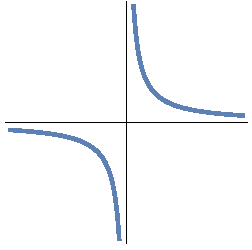
\includegraphics[width=\linewidth]{figures/real-hyperbola.pdf}}
  \noindent 在代数闭域上, 这来自 $xy-1$ 不可约这一事实. 不过, 也可以证明 $X$ 在任意无限域上不可约, 其中包括 $\mathbb{R}$ (Exercise~\ref{ex:hyperbola-irreducible-over-infinite-field}).

  那么, 这个例子中我们的直觉为什么失灵了呢? 答案是 $\mathbb{R}$ 上的解并未反映全貌. 如果拓宽视野, 考虑 $xy-1$ 在 $\mathbb{R}$ 的代数闭包即 $\mathbb{C}$ 上的零点, 就会发现这两\textquotedbl{}块\textquotedbl{}实际上通过复数解相连接. 例如, 可以沿着复数解集
  \[
    \{(e^{\pi\mathrm{i}\theta},e^{-\pi\mathrm{i}\theta})\mid\theta\in[0,1]\}
  \]
  从上面一块中的点 $(1,1)$ 走到下面一块中的点 $(-1,-1)$.

  \BookPairedFigure
    {受这一观察启发, 我们试画 $\mathcal{V}(xy-1)\subseteq\mathbb{A}^{2}_{\mathbb{C}}$. 这有些困难, 因为 $\mathbb{A}^{2}_{\mathbb{C}}$ 在实数上是四维的: $\mathbb{A}^{2}_{\mathbb{C}}=\mathbb{C}^{2}=\mathbb{R}^{4}$. 不过, 通过映入 $\mathbb{R}^{3}$, 可以说明 (Exercise~\ref{ex:complex-hyperbola-real-surface}) 复数解可以与\hyperref[fig:complex-hyperbola]{右图}中的曲面对应起来. 图中还画出了实双曲线和连接 $(1,1)$ 与 $(-1,-1)$ 的路径.}
    {\phantomsection\label{fig:complex-hyperbola}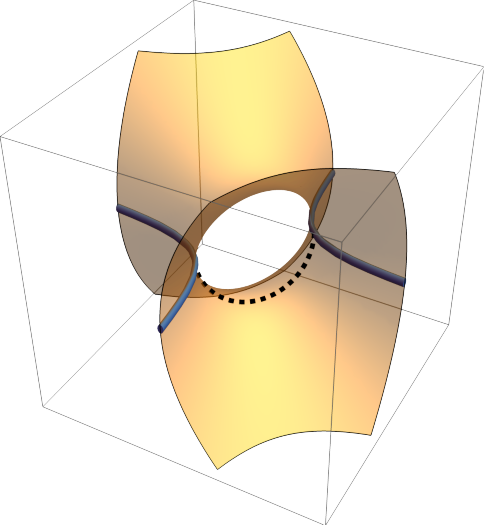
\includegraphics[width=\linewidth]{figures/complex-hyperbola.png}}
  \noindent 因此, 复数情形的图像更接近我们直观上所预期的不可约簇: 它只由一\textquotedbl{}块\textquotedbl{}组成.

  这个例子说明, 在代数几何中利用 $\mathbb{R}$ 上的几何直觉固然重要, 但这样做未必能看到全貌. 只有在能用代数论证加以证明的范围内, 才应当信赖这一直觉.
\end{Example}

有一类特殊的不可约仿射簇只由一个点组成: $X=\{a\}\subseteq\mathbb{A}^{n}$. 由于单点在簇中 (按包含关系) 是极小的, 而 $\mathcal{V}$ 和 $\mathcal{I}$ 算子反转包含关系, 这暗示单点的消没理想应是极大理想. 已知极大理想是特殊的素理想. 这一猜想确实成立, 而且还能说得更多.

\begin{Proposition}{单点与极大理想}\leavevmode\label{prop:single-points-and-maximal-ideals}
  设 $I\subseteq K[x_{1},\ldots,x_{n}]$ 是一个理想. 下列条件等价.
  \begin{enumerate}[label=(\roman*),ref=(\roman*)]
    \item\label{item:maximal-ideal-as-vanishing-ideal-of-singleton} 对某个点 $a=(a_{1},\ldots,a_{n})\in\mathbb{A}^{n}$, 有 $I=\mathcal{I}(\{a\})$.
    \item\label{item:maximal-ideal-as-coordinate-differences} 对某些 $a_{1},\ldots,a_{n}\in K$, 有 $I=\langle x_{1}-a_{1},\ldots,x_{n}-a_{n}\rangle$.
    \item\label{item:maximal-ideal-quotient-is-k} $K[x_{1},\ldots,x_{n}]/I\cong K$.
    \item\label{item:maximal-ideal-condition} $I$ 是极大理想.
  \end{enumerate}
\end{Proposition}

\begin{Proof}
  \ref{item:maximal-ideal-as-vanishing-ideal-of-singleton} 蕴含 \ref{item:maximal-ideal-as-coordinate-differences} 是 Exercise~\ref{ex:vanishing-ideal-of-a-single-point}. \ref{item:maximal-ideal-as-coordinate-differences} 蕴含 \ref{item:maximal-ideal-quotient-is-k} 是 Exercise~\ref{ex:quotient-evaluation-at-point}. \ref{item:maximal-ideal-quotient-is-k} 蕴含 \ref{item:maximal-ideal-condition} 可由 Proposition~\ref{prop:prime-maximal-quotient-characterization} 得出. 因此只需证明 \ref{item:maximal-ideal-condition} 蕴含 \ref{item:maximal-ideal-as-vanishing-ideal-of-singleton}. 假设 $I$ 是极大理想. 由于极大理想都是根理想, 零点定理蕴含 $I=\mathcal{I}(\mathcal{V}(I))$. 要证明 \ref{item:maximal-ideal-as-vanishing-ideal-of-singleton}, 必须证明 $\mathcal{V}(I)$ 是单点. 反设 $\mathcal{V}(I)$ 不是单点. 有两种情形: $\mathcal{V}(I)=\varnothing$ 或 $\mathcal{V}(I)$ 含不止一个点. 若 $\mathcal{V}(I)=\varnothing$, 则
  \[
    I=\mathcal{I}(\mathcal{V}(I))=K[x_{1},\ldots,x_{n}],
  \]
  与 $I$ 的极大性矛盾. 另一方面, 若 $\mathcal{V}(I)$ 含不止一个点, 任取点 $a\in\mathcal{V}(I)$, 并注意 $\varnothing\subsetneq\{a\}\subsetneq\mathcal{V}(I)$ 是仿射簇的严格包含关系. 应用 Proposition~\ref{prop:operators-reverse-inclusions}, 得到
  \[
    K[x_{1},\ldots,x_{n}]\supsetneq\mathcal{I}(\{a\})
      \supsetneq\mathcal{I}(\mathcal{V}(I))=I,
  \]
  这也与 $I$ 的极大性矛盾.
\end{Proof}

注意, \ref{item:maximal-ideal-quotient-is-k} 与 \ref{item:maximal-ideal-condition} 的等价性是纯代数陈述, 在非代数闭域上不成立. 例如, 理想 $\langle x^{2}+1\rangle$ 在 $\mathbb{R}[x]$ 中是极大的, 尽管
\[
  \mathbb{R}[x]/\langle x^{2}+1\rangle\cong\mathbb{C}\not\cong\mathbb{R}.
\]
这一观察反映出 $\langle x^{2}+1\rangle\subseteq\mathbb{R}[x]$ 不是消没理想.

本节最后, 我们描述一部更细致的理想与簇之间的词典. 如前所见, 零点定理蕴含 $\mathcal{V}$ 算子给出 $K[x_{1},\ldots,x_{n}]$ 中的根理想与 $\mathbb{A}^{n}$ 中的仿射簇之间的双射, 其逆是 $\mathcal{I}$ 算子 (Corollary~\ref{cor:radical-ideals-affine-varieties-bijection}). 现在进一步细化这一双射, 把素理想和极大理想也包括进来.

\begin{Proposition}{理想与簇之间更细致的词典}\leavevmode\label{prop:refined-ideals-varieties-dictionary}
  算子 $\mathcal{V}$ 和 $\mathcal{I}$ 是互为逆映射并反转包含关系的双射, 它们建立了下列理想层次与簇的层次之间的对应:
  \[
    \begin{array}{c@{\quad}c@{\quad}c}
      \{K[x_{1},\ldots,x_{n}]\text{ 中的根理想}\}&\longleftrightarrow&
         \{\mathbb{A}^{n}\text{ 中的仿射簇}\}\\
      \rotatebox[origin=c]{90}{$\subseteq$}&&\rotatebox[origin=c]{90}{$\subseteq$}\\
      \{K[x_{1},\ldots,x_{n}]\text{ 中的素理想}\}&\longleftrightarrow&
         \{\mathbb{A}^{n}\text{ 中的不可约簇}\}\\
      \rotatebox[origin=c]{90}{$\subseteq$}&&\rotatebox[origin=c]{90}{$\subseteq$}\\
      \{K[x_{1},\ldots,x_{n}]\text{ 中的极大理想}\}&\longleftrightarrow&
         \{\mathbb{A}^{n}\text{ 中的点}\}.
    \end{array}
  \]
\end{Proposition}

\begin{Proof}
  若 $I$ 是根理想且 $X=\mathcal{V}(I)$, 则零点定理蕴含 $I=\mathcal{I}(X)$. 因此, 根理想与仿射簇之间的双射反转包含关系, 正是 Proposition~\ref{prop:operators-reverse-inclusions} 中的最后一个断言. 要证明 $\mathcal{V}$ 和 $\mathcal{I}$ 限制后给出素理想与不可约簇之间的双射, 只需注意 $I=\mathcal{I}(X)$ 是素理想当且仅当 $X=\mathcal{V}(I)$ 不可约 (Proposition~\ref{prop:irreducible-iff-vanishing-ideal-prime}). 要证明 $\mathcal{V}$ 和 $\mathcal{I}$ 限制后给出极大理想与单点之间的双射, 只需注意 $I=\mathcal{I}(X)$ 是极大理想当且仅当 $X=\mathcal{V}(I)$ 是单点 (Proposition~\ref{prop:single-points-and-maximal-ideals}).
\end{Proof}

\BookExerciseHeading
\begin{BookExercises}
  \item\label{ex:affine-space-is-irreducible} 证明仿射空间在任意无限域上都是不可约的.
  \item\label{ex:irreducible-varieties-over-finite-fields} 说明为什么有限域 (它不可能是代数闭域) 上的仿射簇不可约当且仅当它只含一个点.
  \item\label{ex:coordinate-axes-variety-reducible} 证明 $\mathcal{V}(xy)\subseteq\mathbb{A}^{2}$ 可约.
  \item\label{ex:irreducible-variety-in-finite-union} 设 $X$ 是不可约仿射簇, 并假设
    \[
      X=\bigcup_{i=1}^{r}X_{i},
    \]
    其中每个 $X_{i}$ 都是仿射簇. 证明对某个 $i$, 有 $X=X_{i}$.
  \item\label{ex:sum-of-squares-real-and-complex-irreducibility} 证明仿射簇 $\mathcal{V}(x^{2}+y^{2})\subseteq\mathbb{A}^{2}$ 在 $\mathbb{R}$ 上不可约, 但在 $\mathbb{C}$ 上可约.
  \item\label{ex:real-irreducible-polynomial-with-reducible-variety} 考虑函数 $f=(x^{2}+1)(x^{2}-1)^{2}+y^{2}\in\mathbb{R}[x,y]$.
    \begin{enumerate}[label=(\alph*)]
      \item 用 Eisenstein 判别法证明 $f$ 不可约.
      \item 证明 $\mathcal{V}(f)$ 可约, 由两个不同的点组成.
    \end{enumerate}
  \item\label{ex:hyperbola-irreducible-over-infinite-field} 设 $K$ 是无限域. 本题证明
    \[
      X=\mathcal{V}(xy-1)\subseteq\mathbb{A}^{2}_{K}
    \]
    的不可约性.
    \begin{enumerate}[label=(\alph*)]
      \item 利用 $\mathcal{I}$ 和 $\mathcal{V}$ 的性质证明 $\mathcal{I}(X)\supseteq\langle xy-1\rangle$.
      \item 证明 $\mathcal{I}(X)\subseteq\langle xy-1\rangle$, 可以采用以下策略.
        \begin{enumerate}[label=\roman*.]
          \item 设 $f\in\mathcal{I}(X)$. 证明对某些 $k\in\mathbb{N}$ 和 $g\in K[x]$, 有
          \[
            x^{k}f-g\in\langle xy-1\rangle.
          \]
          \item 利用 $f\in\mathcal{I}(X)$, 证明 $g$ 是零多项式.
          \item 利用 $x^{k}f\in\langle xy-1\rangle$, 证明 $f\in\langle xy-1\rangle$.
        \end{enumerate}
      \item 证明 $\langle xy-1\rangle$ 是素理想, 并用这一点说明为什么 $X$ 不可约.
    \end{enumerate}
  \item\label{ex:complex-hyperbola-real-surface} Example~\ref{ex:hyperbola-is-irreducible} 中画的曲面是实仿射簇
    \[
      Y=\mathcal{V}(uv+w^{2}-1)\subseteq\mathbb{A}^{3}_{\mathbb{R}}.
    \]
    设 $X=\mathcal{V}(xy-1)\subseteq\mathbb{A}^{2}_{\mathbb{C}}$.
    \begin{enumerate}[label=(\alph*)]
      \item 证明 $X=\{(re^{\mathrm{i}\theta},(re^{\mathrm{i}\theta})^{-1})\mid r\in\mathbb{R}_{>0},\ 0\leq\theta<2\pi\}$.
      \item 定义函数 $F:X\to\mathbb{A}^{3}_{\mathbb{R}}$, 把 $(re^{\mathrm{i}\theta},(re^{\mathrm{i}\theta})^{-1})\in X$ 送到
        \[
          \left(\frac{r^{2}-1}{2r}+\frac{r^{2}+1}{2r}\cos\theta,\
            \frac{1-r^{2}}{2r}+\frac{r^{2}+1}{2r}\cos\theta,\
            \frac{r^{2}+1}{2r}\sin\theta\right).
        \]
        证明 $F$ 是从 $X$ 到 $Y$ 的双射.
    \end{enumerate}
\end{BookExercises}

\par\smallskip
{\footnotesize
\noindent\textbf{开放获取.} 本章按照
\href{http://creativecommons.org/licenses/by-nc/4.0/}{Creative Commons Attribution-NonCommercial 4.0 International License}
的条款授权. 该许可允许以任何媒介或格式进行非商业性使用, 分享, 改编, 分发和复制, 但须对原作者和来源作适当署名, 提供 Creative Commons 许可的链接, 并说明是否作了修改.

\noindent
\begin{minipage}[t]{.17\linewidth}
  \vspace{0pt}
\includegraphics[width=.9\linewidth]{figures/source-cc-by-nc.png}
\end{minipage}\hfill
\begin{minipage}[t]{.81\linewidth}
  \vspace{0pt}本章的图片或其他第三方材料均纳入本章的 Creative Commons 许可, 除非材料的署名行另有注明. 如果材料未纳入本章的 Creative Commons 许可, 且您拟进行的使用未获法律规定的许可或超出允许使用的范围, 则须直接向著作权持有人取得许可.
\end{minipage}\par}

\section{不可约分解}\label{sec:irreducible-decompositions}

上一节介绍了仿射簇不可约性的概念. 本节证明一个基本事实: 每个仿射簇都是由不可约仿射簇组成的唯一一个有限集合中各簇的并. 这是 $K[x_{1},\ldots,x_{n}]$ 是 Noether 环这一代数事实的最重要推论之一.

如果 $X$ 可约, 那么可以把 $X$ 写成仿射簇 $X_{1},X_{2}\subsetneq X$ 的并, 而 $X_{1}$ 和 $X_{2}$ 本身也可能可约. 进一步分解 $X_{1}$ 和 $X_{2}$, 就可以把 $X$ 拆成越来越多的仿射簇的并, 直到组成部分都不可约才停止. 这一过程类似于逐步把整数分解成素因数, 或把多项式分解成不可约因子. 下面的命题表明, 与整数的素因数分解或多项式的不可约分解一样, 这一过程最终会终止, 而以这种方式得到的分解是唯一的.

\begin{BookPropositionDefinition}[不可约分解]\leavevmode\label{prop:irreducible-decomposition}
  设 $X\subseteq\mathbb{A}^{n}$ 为非空仿射簇. 则存在不可约仿射簇 $X_{1},\ldots,X_{r}\subseteq X$, 使得对任意 $i\ne j$ 都有 $X_{i}\nsubseteq X_{j}$, 并且
  \begin{equation}\label{eq:irreducible-components-union}
    X=\bigcup_{i=1}^{r}X_{i}.
  \end{equation}
  此外, 除排列顺序外, 不可约仿射簇 $X_{1},\ldots,X_{r}$ 是唯一的. 我们称它们为 $X$ 的\textbf{不可约分支}, 称 \eqref{eq:irreducible-components-union} 为 $X$ 的\textbf{不可约分解}.
\end{BookPropositionDefinition}

这里应当强调, 不可约分支的数目有限, 以及对所有 $i\ne j$ 都有 $X_{i}\nsubseteq X_{j}$, 这两点对不可约分解的唯一性都至关重要. 为说明原因, 考虑抛物线 $X=\mathcal{V}(y-x^{2})\subseteq\mathbb{A}^{2}$. 因为 $X$ 已经不可约, 它的不可约分解只含一个分支. 另一方面, 若不要求 $X_{i}$ 的数目有限, 把 $X$ 写成它的所有点的并,
\[
  X=\bigcup_{p\in X}\{p\},
\]
就会得到另一个不可约分解. 如果不要求对所有 $i\ne j$ 都有 $X_{i}\nsubseteq X_{j}$, 那么也能得到不同的不可约分解, 例如
\[
  X=\{(0,0)\}\cup X.
\]

\begin{Proof}\unskip\textbf{ of Proposition~\ref{prop:irreducible-decomposition}}\quad
  我们先证明存在性, 再证明唯一性.

  (存在性) 反设 $X\subseteq\mathbb{A}^{n}$ 是一个没有有限不可约分解的非空仿射簇. 特别地, 这意味着 $X$ 不是不可约的, 所以可以写成
  \[
    X=X_{1}\cup X_{1}'\qquad\text{其中某些 }X_{1},X_{1}'\subsetneq X.
  \]
  如果 $X_{1}$ 和 $X_{1}'$ 都有有限不可约分解, 那么这两个分解的并将给出 $X$ 的一个有限不可约分解, 与假设相矛盾. 所以 $X_{1}$ 与 $X_{1}'$ 中必有一个没有有限不可约分解. 不妨设 $X_{1}$ 没有有限不可约分解, 写成
  \[
    X_{1}=X_{2}\cup X_{2}'\qquad\text{其中某些 }X_{2},X_{2}'\subsetneq X.
  \]
  同样, 因为 $X_{1}$ 没有有限不可约分解, 所以 $X_{2}$ 和 $X_{2}'$ 中至少有一个没有有限不可约分解. 假设 $X_{2}$ 没有有限不可约分解, 写成
  \[
    X_{2}=X_{3}\cup X_{3}'\qquad\text{其中某些 }X_{3},X_{3}'\subsetneq X.'
  \]
  如此继续, 就在 $\mathbb{A}^{n}$ 中构造出一条相互嵌套的无限仿射簇链:
  \[
    X\supsetneq X_{1}\supsetneq X_{2}\supsetneq X_{3}\supsetneq\cdots.
  \]
  根据 Proposition~\ref{prop:operators-reverse-inclusions}, 这给出 $K[x_{1},\ldots,x_{n}]$ 中一条相互嵌套的无限理想链:
  \[
    \mathcal{I}(X)\subsetneq\mathcal{I}(X_{1})\subsetneq\mathcal{I}(X_{2})
      \subsetneq\mathcal{I}(X_{3})\subsetneq\cdots,
  \]
  这与 $K[x_{1},\ldots,x_{n}]$ 是 Noether 环 (Corollary~\ref{cor:polynomial-rings-are-noetherian}) 矛盾. 这个矛盾蕴含每个仿射簇 $X\subseteq\mathbb{A}^{n}$ 都必定至少有一个有限不可约分解.

  (唯一性) 设
  \[
    X=\bigcup_{i=1}^{r}X_{i}=\bigcup_{j=1}^{s}Y_{j}
  \]
  是 $X$ 的两个不可约分解. 我们必须证明 $r=s$, 且必要时重新排列后, 对每个 $i$ 都有 $X_{i}=Y_{i}$. 不妨设 $r\geq s$.

  因为 $X_{1}\subseteq X$, 有
  \[
    X_{1}=X_{1}\cap X=X_{1}\cap\left(\bigcup_{j=1}^{s}Y_{j}\right)
      =\bigcup_{j=1}^{s}(X_{1}\cap Y_{j}).
  \]
  由于 $X_{1}$ 不可约, 可得对某个 $j$ 有 $X_{1}=X_{1}\cap Y_{j}$ (Exercise~\ref{ex:irreducible-variety-in-finite-union}). 重新排列 $Y_{1},\ldots,Y_{s}$, 可设 $X_{1}=X_{1}\cap Y_{1}$, 这蕴含 $X_{1}\subseteq Y_{1}$.

  同理, 由于 $Y_{1}\subseteq X$, 有
  \[
    Y_{1}=Y_{1}\cap X=Y_{1}\cap\left(\bigcup_{i=1}^{r}X_{i}\right)
      =\bigcup_{i=1}^{r}(Y_{1}\cap X_{i}),
  \]
  所以对某个 $i$ 有 $Y_{1}=Y_{1}\cap X_{i}$, 即 $Y_{1}\subseteq X_{i}$. 由此得 $X_{1}\subseteq Y_{1}\subseteq X_{i}$. 根据不可约分解的定义, 对任意 $i\ne1$ 都有 $X_{1}\nsubseteq X_{i}$, 所以必有 $i=1$. 包含关系 $X_{1}\subseteq Y_{1}\subseteq X_{1}$ 蕴含 $X_{1}=Y_{1}$.

  用 $X_{2}$ 代替 $X_{1}$ 重复这一论证, 可知对某个 $j$ 有 $X_{2}=Y_{j}$. 因为 $X_{2}\ne X_{1}$, 不可能有 $j=1$. 于是, 重新排列 $Y_{2},\ldots,Y_{s}$ 后, 可设 $X_{2}=Y_{2}$. 如此继续, 可证明对每个 $i\in\{1,\ldots,r\}$ 都有 $X_{i}=Y_{i}$. 特别地, 这证明了 $r\leq s$. 由于已经假定 $r\geq s$, 故 $r=s$, 且对所有 $i$ 都有 $X_{i}=Y_{i}$.
\end{Proof}

\begin{Example}{一个交集的不可约分支}\leavevmode\label{ex:irreducible-components-of-quadric-intersection}
  考虑仿射簇
  \[
    X=\mathcal{V}(2x^{2}+2y^{2}-z^{2}-1,x^{2}+y^{2}-1)
      \subseteq\mathbb{A}^{3}_{\mathbb{C}}.
  \]
  \BookPairedFigure
    {注意 $X=Y_{1}\cap Y_{2}$, 其中
     \[
       Y_{1}=\mathcal{V}(2x^{2}+2y^{2}-z^{2}-1)
     \]
     与
     \[
       Y_{2}=\mathcal{V}(x^{2}+y^{2}-1).
     \]
     为了对簇 $X$ 建立一些直觉, 来看 $K=\mathbb{R}$ 时的图形. 在这种情形下, $Y_{1}$ 是单叶双曲面, $Y_{2}$ 是圆柱面, 如\hyperref[fig:quadric-intersection]{右图}所示. 从图中可看出, 它们的交 $X$ 由两个圆组成.}
    {\phantomsection\label{fig:quadric-intersection}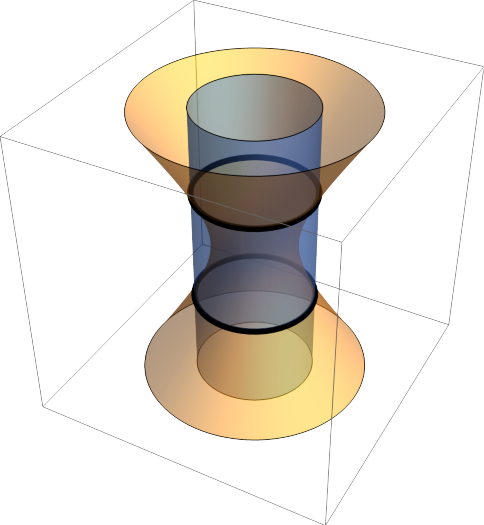
\includegraphics[width=\linewidth]{figures/quadric-intersection-two-circles.png}}
  \noindent 人们或许自然会猜测这两个圆是 $X$ 的不可约分支. 下面用代数方法验证这一直觉.

  如果 $(a,b,c)\in X$, 则其坐标满足
  \[
    2a^{2}+2b^{2}-c^{2}=1\qquad\text{且}\qquad a^{2}+b^{2}=1.
  \]
  从第一个等式中减去第二个等式的两倍, 可知这两个等式成立当且仅当
  \[
    c^{2}=1\qquad\text{且}\qquad a^{2}+b^{2}=1.
  \]
  因为 $c^{2}=1$ 当且仅当 $c=\pm1$, 所以
  \[
    \begin{aligned}
      X&=\{(a,b,1)\mid a^{2}+b^{2}=1\}\cup\{(a,b,-1)\mid a^{2}+b^{2}=1\}\\
       &=\underbrace{\mathcal{V}(x^{2}+y^{2}-1,z-1)}_{X_{1}}\cup
         \underbrace{\mathcal{V}(x^{2}+y^{2}-1,z+1)}_{X_{2}}.
    \end{aligned}
  \]
  在实数上, $X_{1}$ 和 $X_{2}$ 正是\hyperref[fig:quadric-intersection]{上图}所画的两个圆.

  为了证明 $X_{1}$ 和 $X_{2}$ 确实是 $X$ 的不可约分支, 还要证明它们各自不可约. 虽然这一事实可以在 $\mathbb{R}$ 上证明, 但在诸如 $\mathbb{C}$ 这样的代数闭域上证明要简单得多. 特别地, 在 $\mathbb{C}$ 上, 根据 Proposition~\ref{prop:vanishing-set-of-prime-ideal-is-irreducible}, 只需注意
  \[
    \langle x^{2}+y^{2}-1,z+1\rangle,\quad
    \langle x^{2}+y^{2}-1,z-1\rangle\subseteq\mathbb{C}[x,y,z]
  \]
  都是素理想. 读者不妨自行验证这一点 (见 Exercise~\ref{ex:circle-in-plane-prime-ideal}).
\end{Example}

一般而言, 判定一个簇的不可约分支并不容易, 尤其当该簇由含有许多变量的许多多项式描述, 因而无法画图来利用几何直觉时. 不过, 在簇由单个多项式 $f$ 定义的特殊情形下, $\mathcal{V}(f)$ 的不可约分解与 $f$ 的不可约分解密切相关.

\begin{Proposition}{$\mathcal{V}(f)$ 的不可约分解}\leavevmode\label{prop:hypersurface-irreducible-components}
  \strut\par\nopagebreak[4]\noindent
  如果 $f\in K[x_{1},\ldots,x_{n}]$ 的不同不可约因子为 $q_{1},\ldots,q_{m}$, 则 $\mathcal{V}(f)$ 的不可约分解为
  \[
    \mathcal{V}(f)=\mathcal{V}(q_{1})\cup\cdots\cup\mathcal{V}(q_{m}).
  \]
\end{Proposition}

\begin{Proof}
  由零点定理可知
  \[
    \mathcal{V}(f)=\mathcal{V}\bigl(\sqrt{\langle f\rangle}\bigr).
  \]
  应用 Proposition~\ref{prop:radicals-of-principal-ideals}, 可知 $\sqrt{\langle f\rangle}=\langle q_{1}\cdots q_{m}\rangle$, 所以
  \[
    \mathcal{V}(f)=\mathcal{V}(q_{1}\cdots q_{m}).
  \]
  因为 $q_{1}\cdots q_{m}$ 在某点为零当且仅当其中一个 $q_{i}$ 在该点为零, 所以
  \begin{equation}\label{eq:hypersurface-irreducible-decomposition}
    \mathcal{V}(f)=\mathcal{V}(q_{1})\cup\cdots\cup\mathcal{V}(q_{m}).
  \end{equation}
  由于每个 $q_{i}$ 都不可约, Proposition~\ref{prop:vanishing-set-of-prime-ideal-is-irreducible} 蕴含每个 $\mathcal{V}(q_{i})$ 都不可约.

  为完成证明, 必须验证对任意 $i\ne j$ 都有 $\mathcal{V}(q_{i})\nsubseteq\mathcal{V}(q_{j})$. 根据不同不可约因子的定义, 对任意 $i\ne j$ 都有 $q_{i}\nmid q_{j}$. 这蕴含对任意 $i\ne j$ 都有 $\langle q_{i}\rangle\nsupseteq\langle q_{j}\rangle$. 因为每个 $q_{i}$ 都不可约, 所以 $\langle q_{i}\rangle$ 是素理想, 而零点定理蕴含
  \[
    \mathcal{I}(\mathcal{V}(q_{i}))=\mathcal{I}(\mathcal{V}(\langle q_{i}\rangle))
      =\sqrt{\langle q_{i}\rangle}=\langle q_{i}\rangle.
  \]
  因此, 由于对任意 $i\ne j$ 都有 $\mathcal{I}(\mathcal{V}(q_{i}))\nsupseteq\mathcal{I}(\mathcal{V}(q_{j}))$, Proposition~\ref{prop:operators-reverse-inclusions} 的最后一个断言蕴含对任意 $i\ne j$ 都有 $\mathcal{V}(q_{i})\nsubseteq\mathcal{V}(q_{j})$.
\end{Proof}

\BookPairedNote
  {$K[x_{1},\ldots,x_{n}]$ 中并非每个理想都由单个多项式生成, 很自然会问, 对非主理想 $I$, 怎样计算 $\mathcal{V}(I)$ 的不可约分解? 虽然手算很困难, 但可以借助计算机完成.}
  {关于代数几何中侧重计算和算法的入门介绍, 见 Cox, Little 和 O’Shea 的书 [\ref{bib:cox-little-oshea}].}
\noindent 特别地, 给定一组生成元 $I=\langle f_{1},\ldots,f_{k}\rangle$, 有利用 Gröbner 基计算 $\mathcal{V}(I)$ 的不可约分解的有效算法. 本书选择不介绍这些计算工具, 而着重讨论代数与几何之间的词典中较偏理论的方面.

\BookExerciseHeading
\begin{BookExercises}
  \item\label{ex:irreducible-components-crossing-lines} 设 $K$ 是特征不等于 $2$ 的无限域. 证明 $\mathcal{V}(x^{2}-y^{2})\subseteq\mathbb{A}^{2}$ 的不可约分解为
    \[
      \mathcal{V}(x^{2}-y^{2})=\mathcal{V}(x+y)\cup\mathcal{V}(x-y).
    \]
    如果特征等于 $2$, 会有什么变化?
  \item\label{ex:circle-in-plane-prime-ideal} 证明
    \[
      \frac{\mathbb{C}[x,y,z]}{\langle x^{2}+y^{2}-1,z-1\rangle}
        \cong\frac{\mathbb{C}[x,y]}{\langle x^{2}+y^{2}-1\rangle}.
    \]
    据此得出 $\langle x^{2}+y^{2}-1,z-1\rangle$ 是素理想.
  \item\label{ex:quadric-intersection-real-components} 下列仿射簇的不可约分支是什么?
    \[
      \mathcal{V}(x^{2}+y^{2}+z^{2}-2z,x^{2}+y^{2}-z^{2})
        \subseteq\mathbb{A}^{3}_{\mathbb{R}}.
    \]
    (提示: 画出两个曲面, 看它们怎样相交.)
  \item\label{ex:quadric-intersection-complex-components} 求下列仿射簇的不可约分解:
    \[
      \mathcal{V}(x^{2}+y^{2}+z^{2}-2z,x^{2}+y^{2}-z^{2})
        \subseteq\mathbb{A}^{3}_{\mathbb{C}}.
    \]
    (提示: 有三个不可约分支. 复数情形的图像与上一道习题的实数情形有何不同?)
  \item\label{ex:polynomial-curve-two-irreducible-components} 求下列仿射簇的不可约分解:
    \[
      \mathcal{V}(xy+z,x^{2}-x+y^{2}+yz)\subseteq\mathbb{A}^{3}_{\mathbb{C}}.
    \]
    (提示: 有两个不可约分支.)
\end{BookExercises}


\chapter{坐标环}\label{chap:coordinate-rings}

\noindent\textbf{第 \thechapter{} 章学习目标}
\begin{itemize}
  \item 分别用多项式函数和商环定义仿射簇 $X$ 的坐标环 $K[X]$.
  \item 定义 $K$-代数, 并说明怎样把有限生成的 $K$-代数与多项式环的商等同起来.
  \item 判定一个环是否既约, 并借助商环判定理想是否为根理想.
  \item 用代数性质刻画坐标环: 它们正是有限生成的既约 $K$-代数.
  \item 在具体例子中, 给定一个有限生成的既约 $K$-代数, 求以它为坐标环的仿射簇.
\end{itemize}

第~\ref{chap:varieties-and-ideals}~章的工作给出了在代数与几何两界之间往返的方法, 其中 $\mathcal{V}$ 和 $\mathcal{I}$ 算子是 $\mathbb{A}^{n}$ 中的仿射簇与 $K[x_{1},\ldots,x_{n}]$ 中的根理想之间互逆的双射. 但在代数一侧, 理想还有一个我们尚未用到的特殊作用: 正是对 $K[x_{1},\ldots,x_{n}]$ 的这些子集, 可以取商得到一个环. 若 $X\subseteq\mathbb{A}^{n}$ 是一个仿射簇, 那么应当怎样从仿射簇 $X$ 的角度解释 $K[x_{1},\ldots,x_{n}]$ 对 $\mathcal{I}(X)$ 取商所得的环?

如本章所见, 答案是这个商环自然同构于 $X$ 的坐标环, 即由从 $X$ 到基域 $K$ 的多项式函数所组成的环 $K[X]$. 在第~\ref{sec:polynomial-functions-on-affine-varieties}~节给出这些对象的精确定义后, 我们将有一种从几何走向代数的新方法:
\[
  \begin{aligned}
    \{\text{仿射簇}\}&\to\{\text{环}\}\\
    X&\mapsto K[X].
  \end{aligned}
\]
照例, 我们要问这个对应是否是一本双向词典. 一开始并不是, 因为并非每个环都是某个 $X$ 的 $K[X]$. 为了从代数上刻画哪些环可以成为坐标环, 我们将定义 $K$-代数这一概念, 并研究它的关键代数性质. $K$-代数是一类特殊的环, 包括多项式环及其商环. 本章最后得出的结论是: 一个环恰好在它是有限生成的既约 $K$-代数时才是某个仿射簇的坐标环.

\par\smallskip
{\footnotesize
\noindent\textcopyright{} The Author(s) 2025\par
\noindent E. Clader, D. Ross, \emph{Beginning in Algebraic Geometry}, Undergraduate Texts in Mathematics,
\href{https://doi.org/10.1007/978-3-031-88819-9_4}{\nolinkurl{https://doi.org/10.1007/978-3-031-88819-9_4}}.\par}

\section{仿射簇上的多项式函数}\label{sec:polynomial-functions-on-affine-varieties}

第~\ref{sec:vanishing-set-operator}~节说明了每个多项式 $f\in K[x_{1},\ldots,x_{n}]$ 都可用来定义函数 $\mathbb{A}^{n}\to K$, 把 $(a_{1},\ldots,a_{n})$ 映到 $f(a_{1},\ldots,a_{n})$. 若 $X\subseteq\mathbb{A}^{n}$ 是一个仿射簇, 就可以把这样的函数的定义域限制到 $X$, 得到一个新函数
\[
  \begin{aligned}
    f|_{X}:X&\to K\\
    (a_{1},\ldots,a_{n})&\mapsto f(a_{1},\ldots,a_{n}).
  \end{aligned}
\]
由这种方式得到的函数 $F:X\to K$ 称为多项式函数.

\begin{Definition}{多项式函数}\leavevmode\label{def:polynomial-function-on-affine-variety}
  设 $X\subseteq\mathbb{A}^{n}$ 是仿射簇. $X$ 上的\textbf{多项式函数}是满足 $F=f|_{X}$ 的函数 $F:X\to K$, 其中 $f\in K[x_{1},\ldots,x_{n}]$ 为某个多项式.
\end{Definition}

\begin{Example}{抛物线上的多项式函数}\leavevmode\label{ex:polynomial-functions-on-parabola}
  设 $X=\mathcal{V}(y-x^{2})\subseteq\mathbb{A}^{2}$. 函数
  \[
    \begin{aligned}
      F:X&\to K\\
      (a,b)&\mapsto a+b
    \end{aligned}
  \]
  是多项式函数, 因为
  \[
    F=f|_{X}\qquad\text{其中}\qquad f=x+y\in K[x,y].
  \]
  注意, $f=x+y$ 并不是唯一能给出 $F$ 的多项式. 例如, 由于对所有 $(a,b)\in X$ 都有 $a^{2}=b$, 可知 $F=g|_{X}$, 其中 $g=x+x^{2}$, 同时 $F=h|_{X}$, 其中 $h=x+2y-x^{2}$.
\end{Example}

\begin{Example}{坐标函数}\leavevmode\label{ex:coordinate-functions}
  设 $X\subseteq\mathbb{A}^{n}$ 是仿射簇. 对每个 $i\in\{1,\ldots,n\}$, $X$ 上的第 $i$ 个坐标函数是
  \[
    \begin{aligned}
      C_{i}:X&\to K\\
      (a_{1},\ldots,a_{n})&\mapsto a_{i}.
    \end{aligned}
  \]
  坐标函数是多项式函数, 因为 $C_{i}$ 是多项式 $x_{i}\in K[x_{1},\ldots,x_{n}]$ 所对应函数的限制.
\end{Example}

\begin{Example}{空函数}\leavevmode\label{ex:empty-polynomial-function}
  若 $X=\varnothing\subseteq\mathbb{A}^{n}$, 那么只有一个函数 $F:\varnothing\to K$, 即空函数. 此外, 把定义域限制到空集时, 每个函数 $\mathbb{A}^{n}\to K$ 都给出空函数. 特别地, 这意味着空函数是仿射簇 $\varnothing\subseteq\mathbb{A}^{n}$ 上唯一的多项式函数.
\end{Example}

从以上讨论应当很清楚, 构造 $X\subseteq\mathbb{A}^{n}$ 上的多项式函数, 只须选取任意多项式 $f\in K[x_{1},\ldots,x_{n}]$, 考虑 $\mathbb{A}^{n}$ 上相应的函数, 再把其定义域限制到 $X$. 那么, 为什么定义 $X$ 上的多项式函数时, 我们却似乎采用了相反的方式, 从 $F$ 出发, 再寻找一个限制到 $X$ 后等于 $F$ 的 $f$?

这样做的主要原因是: 给定多项式函数 $F:X\to K$, 可能有许多多项式 $f\in K[x_{1},\ldots,x_{n}]$ 满足 $F=f|_{X}$, 我们并不想把它们看成 $X$ 上不同的多项式函数. 这一点在 Example~\ref{ex:polynomial-functions-on-parabola} 中已经很明显, 其中不同的多项式 $f,g,h\in K[x,y]$ 都定义了同一个函数 $F:X\to K$. 这里重要的不是多项式 $f\in K[x_{1},\ldots,x_{n}]$, 我们要研究的是函数 $F:X\to K$.

不过, 从 $F$ 出发也有缺点. 视 $F$ 的定义如何给出, 它是否为某个多项式所对应函数的限制, 可能并不显然. 下一个例子说明了这个现象, 也提醒我们不要过早判断一个函数是不是多项式函数.

\begin{Example}{一个不显然是多项式函数的函数}\leavevmode\label{ex:apparently-nonpolynomial-hyperbola-function}
  设 $X=\mathcal{V}(xy-1)\subseteq\mathbb{A}^{2}$. 由于任意 $(a,b)\in X$ 都有 $a\ne0$, 可以考虑如下定义的函数:
  \[
    \begin{aligned}
      F:X&\to K\\
      (a,b)&\mapsto\frac{1}{a}.
    \end{aligned}
  \]
  输出 $\frac{1}{a}$ 并不是关于 $a$ 和 $b$ 的多项式, 这也许会让人猜测 $F$ 不是多项式函数. 然而, 对所有 $(a,b)\in X$ 都有 $ab-1=0$, 这意味着 $\frac{1}{a}=b$, 从而 $F=f|_{X}$, 其中 $f=y\in K[x,y]$.

  更一般地, 任意形如
  \[
    F(a,b)=\frac{f(a,b)}{a^{j}b^{k}}
  \]
  的函数 $F:X\to K$, 其中 $f\in K[x,y]$, $j,k\in\mathbb{N}$, 都是 $X$ 上的多项式函数 (Exercise~\ref{ex:hyperbola-polynomial-function-despite-denominators}).
\end{Example}

对 $X$ 上多项式函数的集合, 可以用通常的方式加乘函数, 从而赋予它环结构:
\[
  \begin{aligned}
    (F+G)(a_{1},\ldots,a_{n})&=F(a_{1},\ldots,a_{n})+G(a_{1},\ldots,a_{n}),\\
    (F\cdot G)(a_{1},\ldots,a_{n})&=F(a_{1},\ldots,a_{n})\cdot G(a_{1},\ldots,a_{n}).
  \end{aligned}
\]
因此, 从一个仿射簇 $X$ 出发, 可以得到一个与之关联的环. 这个环在代数几何的研究中居于核心地位.

\begin{Definition}{坐标环}\leavevmode\label{def:coordinate-ring}
  设 $X\subseteq\mathbb{A}^{n}$ 是仿射簇. $X$ 的\textbf{坐标环}记为 $K[X]$, 是 $X$ 上所有多项式函数构成的环.
\end{Definition}

加法单位元 $0\in K[X]$ 是对所有 $a\in X$ 取值 $0\in K$ 的常函数, 乘法单位元是对所有 $a\in X$ 取值 $1\in K$ 的常函数. 这两个函数分别来自多项式 $0,1\in K[x_{1},\ldots,x_{n}]$: $0=0|_{X}$ 且 $1=1|_{X}$.

给定仿射簇 $X$, 能否计算 $K[X]$? 换句话说, 能否把 $K[X]$ 与一个更熟悉的环等同起来? 下面的结果把坐标环表示为一个商环, 朝这个方向迈出一步.

\begin{Proposition}{坐标环的商环表示}\leavevmode\label{prop:coordinate-ring-as-quotient}
  若 $X\subseteq\mathbb{A}^{n}$ 是仿射簇, 则有典范环同构
  \[
    K[X]=\frac{K[x_{1},\ldots,x_{n}]}{\mathcal{I}(X)}.
  \]
\end{Proposition}

\begin{Proof}
  根据第一同构定理, 只须找到一个以 $\mathcal{I}(X)$ 为核的典范满同态 $\phi:K[x_{1},\ldots,x_{n}]\to K[X]$. 定义 $\phi$ 为
  \[
    \phi(f)=f|_{X}.
  \]
  注意 $(f+g)|_{X}=f|_{X}+g|_{X}$ 且 $(f\cdot g)|_{X}=f|_{X}\cdot g|_{X}$, 可知 $\phi$ 是环同态. 根据定义, $X$ 上每个多项式函数都来自某个 $f\in K[x_{1},\ldots,x_{n}]$, 所以 $\phi$ 是满射. 最后, $f\in\ker\phi$ 当且仅当 $f|_{X}=0$, 这等价于 $f\in\mathcal{I}(X)$. 由此可见 $\ker\phi=\mathcal{I}(X)$.
\end{Proof}

\begin{Example}{仿射空间的坐标环}\leavevmode\label{ex:coordinate-ring-of-affine-space}
  由 Proposition~\ref{prop:polynomial-function-isomorphism}, 以及 $K$ 是代数闭域从而是无限域这一事实, 可知 $K[\mathbb{A}^{n}]=K[x_{1},\ldots,x_{n}]$.
\end{Example}

\begin{Example}{抛物线的坐标环}\leavevmode\label{ex:coordinate-ring-of-parabola}
  在 Example~\ref{ex:polynomial-functions-on-parabola} 中, 我们已经看到, 对 $X=\mathcal{V}(y-x^{2})\subseteq\mathbb{A}^{2}$, 三个多项式
  \[
    f=x+y,\quad g=x+x^{2},\quad\text{以及}\quad h=x-x^{2}+2y
  \]
  都给出同一个多项式函数 $F:X\to K$. 这反映了在商环
  \[
    K[X]=\frac{K[x,y]}{\mathcal{I}(X)}=\frac{K[x,y]}{\langle y-x^{2}\rangle}
  \]
  中有 $[f]=[g]=[h]$. 验算如下: $f-g=y-x^{2}\in\langle y-x^{2}\rangle$ 且 $g-h=2x^{2}-2y\in\langle y-x^{2}\rangle$.
\end{Example}

对一个仿射簇 $X\subseteq\mathbb{A}^{n}$, Definition~\ref{def:coordinate-ring} 和 Proposition~\ref{prop:coordinate-ring-as-quotient} 给出了坐标环 $K[X]$ 的两种不同刻画. 记住这两种解释很重要: 坐标环的元素既应看作函数 $F:X\to K$, 也应看作 $K[x_{1},\ldots,x_{n}]$ 中多项式的等价类. 对任意 $f\in K[x_{1},\ldots,x_{n}]$, Proposition~\ref{prop:coordinate-ring-as-quotient} 中的典范同构将多项式函数 $f|_{X}$ 与等价类 $[f]$ 等同起来.

如本章开篇所说, 我们现在已经给出一种从几何走向代数的新方法, 即为一个仿射簇 $X$ 配上它的坐标环 $K[X]$. 按照几何与代数之间的转换应是一本双向词典这一思想, 我们现在要问从仿射簇到其坐标环的转换能否逆转. 更确切地说, 给定一个环 $R$, 是否存在仿射簇 $X$ 使 $R=K[X]$? 我们将看到, 如果 $R$ 是有限生成的既约 $K$-代数, 答案就是肯定的. 接下来三节将定义并研究这些术语.

\BookExerciseHeading
\begin{BookExercises}
  \item\label{ex:coordinate-ring-of-empty-set} 描述空集上的多项式函数环. $0$ 是什么? $1$ 又是什么?
  \item\label{ex:distinct-polynomials-restrict-to-same-function} 设 $X=\mathcal{V}(x^{2}+y^{2}-2z^{2})\subseteq\mathbb{A}^{3}$. 列出 $K[x,y,z]$ 的三个不同元素, 它们限制后给出 $K[X]$ 中同一个多项式函数; 再列出 $K[x,y,z]$ 的两个元素, 它们限制后给出 $K[X]$ 中不同的多项式函数.
  \item\label{ex:hyperbola-polynomial-function-despite-denominators} 设 $X=\mathcal{V}(xy-1)\subseteq\mathbb{A}^{2}$. 证明任意形如
    \[
      F(a,b)=\frac{f(a,b)}{a^{j}b^{k}}
    \]
    的函数 $F:X\to K$, 其中 $f\in K[x,y]$, $j,k\in\mathbb{N}$, 都是多项式函数.
  \item\label{ex:coordinate-ring-domain-iff-irreducible} 设 $X\subseteq\mathbb{A}^{n}$ 是仿射簇.
    \begin{enumerate}[label=(\alph*),ref=(\alph*)]
      \item\label{item:coordinate-ring-domain-iff-irreducible} 证明 $K[X]$ 是整环当且仅当 $X$ 不可约.
      \item 作为 \ref{item:coordinate-ring-domain-iff-irreducible} 的一个例子, 设 $X=\mathcal{V}(x^{2}-xy)\subseteq\mathbb{A}^{2}$. 找到两个仿射簇 $X_{1}\subsetneq X$ 和 $X_{2}\subsetneq X$ 使 $X=X_{1}\cup X_{2}$, 从而证明 $X$ 可约. 然后, 找到 $K[X]$ 中乘积为零的两个非零函数, 验证 $K[X]$ 不是整环.
    \end{enumerate}
  \item\label{ex:coordinate-ring-of-single-point} 设 $X=\{p\}\subseteq\mathbb{A}^{n}$ 是一个单点. 证明由 $\phi(F)=F(p)$ 定义的函数 $\phi:K[X]\to K$ 是环同构.
  \item\label{ex:coordinate-ring-of-finite-points} 设 $p_{1},\ldots,p_{m}\in\mathbb{A}^{n}$ 是 $\mathbb{A}^{n}$ 中互不相同的点, 并令 $X=\{p_{1},\ldots,p_{m}\}$. 证明函数
    \[
      \begin{aligned}
        \phi:K[X]&\to\overbrace{K\oplus\cdots\oplus K}^{m}\\
        \phi(F)&=(F(p_{1}),\ldots,F(p_{m}))
      \end{aligned}
    \]
    是环同构. (回顾一下, 直和的加法和乘法按分量定义.)
  \item\label{ex:equal-coordinate-functions-on-infinite-variety}
    \begin{enumerate}[label=(\alph*),ref=(\alph*)]
      \item\label{item:equal-coordinate-functions-example} 举出一个无限仿射簇 $X\subseteq\mathbb{A}^{3}$, 使三个坐标函数都是同一个多项式函数.
      \item 证明 \ref{item:equal-coordinate-functions-example} 的解是唯一的.
    \end{enumerate}
\end{BookExercises}

\section{\texorpdfstring{$K$}{K}-代数}\label{sec:k-algebras}

哪些类型的环可以写成某个仿射簇 $X$ 的 $K[X]$? 先考察基域 $K$ 所起的特殊作用, 从而给出这个问题的第一个答案.

为了引出下面的讨论, 考虑 $X=\mathbb{A}^{1}$ 的情形, 此时
\[
  K[\mathbb{A}^{1}]=K[x].
\]
如我们已经详细讨论的, $K[x]$ 是一个环. 不过, 它不只是一个普通的环, 还是 $K$ 上的向量空间, 因为除了能对多项式作加法与乘法, 也能用 $K$ 中的标量乘多项式 (加法和数乘这两个运算满足通常的向量空间公理). 与线性代数入门课程中通常研究的向量空间不同, $K[x]$ 是无限维的, 它的一组基为
\[
  B=\{1,x,x^{2},x^{3},\ldots\}.
\]
尽管如此, 与较熟悉的有限维向量空间一样, $K[x]$ 的每个元素都能唯一地写成 $B$ 中元素的线性组合.

更一般地, 每个坐标环都具有相同的附加结构: 它既是一个环, 又是 $K$ 上的向量空间. 本节建立 $K$-代数的代数基础, 用 $K$-代数将这一结构形式化. (在此提醒读者, 本书假设所有环都是带单位元的交换环.)

\begin{Definition}{$K$-代数}\leavevmode\label{def:k-algebra}
  一个 \textbf{$K$-代数}是一个环 $A$, 连同一个数乘映射
  \[
    \begin{aligned}
      K\times A&\to A\\
      (r,a)&\mapsto r\cdot a
    \end{aligned}
  \]
  满足以下公理.
  \begin{enumerate}[label=\arabic*.]
    \item 对所有 $r\in K$ 和所有 $a,b\in A$, 有 $r\cdot(a+b)=r\cdot a+r\cdot b$.
    \item 对所有 $r,s\in K$ 和所有 $a\in A$, 有 $(r+s)\cdot a=r\cdot a+s\cdot a$.
    \item 对所有 $r,s\in K$ 和所有 $a\in A$, 有 $(rs)\cdot a=r\cdot(s\cdot a)$.
    \item 对所有 $a\in A$, 有 $1\cdot a=a$.
    \item 对所有 $r\in K$ 和所有 $a,b\in A$, 有 $r\cdot(ab)=(r\cdot a)b=a(r\cdot b)$.
  \end{enumerate}
\end{Definition}

\BookPairedNoteLeft
  {为便于读懂 Definition~\ref{def:k-algebra} 中的公理, $K$ 和 $A$ 各自内部的乘积用元素直接并写来表示, 记号\textquotedbl{}$\cdot$\textquotedbl{}只用于数乘.}
  {前四条公理规定 $A$ 构成 $K$ 上的向量空间, 第五条公理说明数乘与 $A$ 中的乘法运算如何相容.}
\noindent 由上述公理可知, 对任意 $a\in A$, 用 $0\in K$ 数乘 $a$ 得到 $0\in A$, 用 $-1\in K$ 数乘 $a$ 得到加法逆元 $-a\in A$. 这也是一般向量空间都具有的性质 (Exercise~\ref{ex:zero-and-negative-one-scalar-action}).

\begin{Example}{多项式环}\leavevmode\label{ex:polynomial-rings-as-k-algebras}
  尤其从代数几何的角度来看, 多项式环 $K[x_{1},\ldots,x_{n}]$ 是 $K$-代数的典型例子. 的确, 除了可以对多项式作加法与乘法, 还可以用 $K$ 中的标量乘多项式, 而 Definition~\ref{def:k-algebra} 中的公理很容易验证.
\end{Example}

\begin{Example}{坐标环}\leavevmode\label{ex:coordinate-rings-as-k-algebras}
  设 $X$ 是一个仿射簇. 坐标环 $K[X]$ 构成一个 $K$-代数. 对任意 $F\in K[X]$ 和 $r\in K$, 定义 $r\cdot F\in K[X]$ 为下式给出的函数:
  \[
    (r\cdot F)(a_{1},\ldots,a_{n})=r\cdot F(a_{1},\ldots,a_{n}),
  \]
  其中右边的乘法是 $K$ 中通常的乘法. 为验证 $r\cdot F$ 确实是 $K[X]$ 的元素, 注意对某个 $f\in K[x_{1},\ldots,x_{n}]$, 有 $F=f|_{X}$, 因而 $r\cdot F=(r\cdot f)|_{X}$. 由于 $r\cdot f\in K[x_{1},\ldots,x_{n}]$, 可见 $r\cdot F\in K[X]$. Definition~\ref{def:k-algebra} 中的公理同样容易验证.
\end{Example}

\begin{Example}{$K$ 的扩张环}\leavevmode\label{ex:extension-rings-as-k-algebras}
  若 $A$ 是以 $K$ 为子环的任意环, 那么 $A$ 自然是一个 $K$-代数, 其中数乘就是 $A$ 中通常的环乘法. 事实上, 在我们的假设下 (环是带单位元的交换环), 每个非平凡的 $K$-代数都以这种方式得到. 更确切地说, 给定任意 $K$-代数 $A\ne\{0\}$, 都有一个典范包含映射 $K\to A$. 经由这个包含映射把 $K$ 看成 $A$ 的子环, 数乘就与 $A$ 中通常的乘法等同起来 (Exercise~\ref{ex:canonical-copy-of-k-in-algebra}). 特别地, 每个非平凡的 $K$-代数都以典范的方式包含一份 $K$.
\end{Example}

\begin{Example}{不是 $K$-代数的例子}\leavevmode\label{ex:integers-not-k-algebra}
  根据 Example~\ref{ex:extension-rings-as-k-algebras}, 任何不包含 $K$ 的非零环都不是 $K$-代数. 例如, 由于 $\mathbb{Z}$ 不包含任何域, 它不是任何域 $K$ 上的 $K$-代数.
\end{Example}

要完整建立 $K$-代数的理论, 还必须指明其间适当的态射. 既然 $K$-代数是带有数乘运算的环, $K$-代数同态就是保持数乘的环同态.

\begin{Definition}{$K$-代数同态}\leavevmode\label{def:k-algebra-homomorphism}
  设 $A$ 和 $B$ 为 $K$-代数. 一个 \textbf{$K$-代数同态} $\phi:A\to B$ 是满足
  \[
    \phi(r\cdot a)=r\cdot\phi(a)
  \]
  的环同态, 其中等式对所有 $r\in K$ 和 $a\in A$ 成立. 若 $\phi$ 有一个同样为 $K$-代数同态的逆, 则称 $\phi$ 是一个 \textbf{$K$-代数同构}, 并记 $A\cong B$.
\end{Definition}

同构似乎比双射要求更强: 不仅逆函数应当存在, 它还必须是 $K$-代数同态. 不过, 与群, 环和域的情形一样, 若 $\phi$ 是双射同态, 那么它的逆自动是同态 (Exercise~\ref{ex:bijective-k-algebra-homomorphism-is-isomorphism}).

\begin{Example}{从多项式环出发的 $K$-代数同态}\leavevmode\label{ex:k-algebra-evaluation-homomorphisms}
  考虑求值映射
  \[
    \begin{aligned}
      \phi:\mathbb{R}[x,y]&\to\mathbb{R}\\
      f(x,y)&\mapsto f(2,3).
    \end{aligned}
  \]
  稍加思考便可看出 $\phi$ 是一个 $\mathbb{R}$-代数同态. 此外, 知道 $\phi$ 是一个 $\mathbb{R}$-代数同态后, 还可看出它完全由 $x$ 和 $y$ 的像决定. 例如, 一旦知道 $\phi(x)=2$ 和 $\phi(y)=3$, 利用 $\phi$ 是保持数乘的环同态这一事实, 可得
  \[
    \phi(5x^{2}y+2y+xy)=5(2)^{2}(3)+2(3)+(2)(3)=72.
  \]
  更一般地, 对任意 $K$-代数 $A$ 和子集 $\{a_{1},\ldots,a_{n}\}\subseteq A$, 存在唯一的 $K$-代数同态
  \[
    \phi:K[x_{1},\ldots,x_{n}]\to A
  \]
  满足对所有 $i$ 都有 $\phi(x_{i})=a_{i}$ (Exercise~\ref{ex:polynomial-ring-map-determined-by-generators}). 这表明, 给出一个 $K$-代数同态 $K[x_{1},\ldots,x_{n}]\to A$ 等价于选定 $a_{1},\ldots,a_{n}\in A$.
\end{Example}

与群和环一样, $K$-代数也有第一同构定理, 它是证明两个 $K$-代数同构的基本工具. 要叙述这一定理, 首先必须定义 $K$-代数的商与子代数.

由于 $K$-代数 $A$ 是一个环, 已知对任何理想 $I\subseteq A$, 都可以构造商环 $A/I$. 下面的结果表明, 商环 $A/I$ 自然地从 $A$ 继承一个 $K$-代数结构.

\begin{Proposition}{商 $K$-代数}\leavevmode\label{prop:quotient-k-algebra}
  设 $A$ 为 $K$-代数. 若 $I\subseteq A$ 是一个理想, 则商环 $A/I$ 是一个 $K$-代数, 其中数乘定义为
  \begin{equation}\label{eq:quotient-algebra-scalar-multiplication}
    r\cdot[a]=[r\cdot a].
  \end{equation}
\end{Proposition}

\begin{Proof}
  我们必须验证 \eqref{eq:quotient-algebra-scalar-multiplication} 给出的数乘是良定义的. 关键在于理想自动对数乘封闭: 若 $a\in I$ 且 $r\in K$, 则
  \[
    r\cdot a=r\cdot(1a)=(r\cdot1)a.
  \]
  其中 $1$ 是 $A$ 的单位元. 由于 $r\cdot1\in A$ 且 $a\in I$, 理想的吸收性蕴含 $(r\cdot1)a\in I$. 因此 $r\cdot a\in I$, 这验证了 $I$ 对数乘封闭.

  由此出发, 要说明数乘是良定义的, 假设 $[a]=[b]$. 则 $a-b\in I$. 利用 $I$ 吸收数乘这一事实, 得 $r\cdot a-r\cdot b=r\cdot(a-b)\in I$, 这表明 $[r\cdot a]=[r\cdot b]$.

  由于 $I$ 是理想, 我们已经知道 $A/I$ 是环. 所以只剩下 Definition~\ref{def:k-algebra} 中的五条公理需要验证. 它们容易由 $A$ 中相应公理的成立得出.
\end{Proof}

现在给出第一同构定理所需的最后一个要素.

\begin{Definition}{子代数}\leavevmode\label{def:k-subalgebra}
  设 $A$ 为 $K$-代数. \textbf{子代数} $B\subseteq A$ 是满足对所有 $r\in K$ 和 $b\in B$ 都有 $r\cdot b\in B$ 的子环.
\end{Definition}

换言之, $K$-代数的一个子集是子代数, 当且仅当它既是子环又对数乘封闭, 因而本身构成一个 $K$-代数. 一个自然的例子是把 $K$-代数 $K[x]$ 作为 $K[x,y]$ 的子代数.

\begin{Theorem}{$K$-代数的第一同构定理}\leavevmode\label{thm:first-isomorphism-theorem-k-algebras}
  若 $\phi:A\to B$ 是一个 $K$-代数同态, 则
  \begin{enumerate}[label=(\roman*)]
    \item $\operatorname{im}(\phi)$ 是 $B$ 的子代数,
    \item $\ker(\phi)$ 是 $A$ 的理想, 并且
    \item 函数
    \[
      \begin{aligned}
        [\phi]:\frac{A}{\ker(\phi)}&\to\operatorname{im}(\phi)\\
        [a]&\mapsto\phi(a)
      \end{aligned}
    \]
    是一个良定义的 $K$-代数同构.
  \end{enumerate}
\end{Theorem}

\begin{Proof}
  见 Exercise~\ref{ex:prove-first-isomorphism-theorem-k-algebras}.
\end{Proof}

\begin{Example}{$\mathbb{C}$ 作为商 $\mathbb{R}$-代数}\leavevmode\label{ex:complex-numbers-as-quotient-real-algebra}
  把 $\mathbb{C}$ 看成 $\mathbb{R}$-代数, 其中数乘是通常的乘法. 令 $\phi$ 为函数
  \[
    \begin{aligned}
      \phi:\mathbb{R}[x]&\to\mathbb{C}\\
      \phi(f)&=f(\mathrm{i}).
    \end{aligned}
  \]
  可以验证 (Exercise~\ref{ex:verify-complex-quotient-real-algebra}) $\phi$ 是以 $\langle x^{2}+1\rangle$ 为核的满 $\mathbb{R}$-代数同态. 因此, 由 Theorem~\ref{thm:first-isomorphism-theorem-k-algebras}, 有 $\mathbb{R}$-代数同构
  \[
    \mathbb{C}\cong\mathbb{R}[x]/\langle x^{2}+1\rangle.
  \]
  作为 $\mathbb{R}$ 上的向量空间, 复数集 $\mathbb{C}$ 有一组基 $\{1,\mathrm{i}\}$, 而商 $\mathbb{R}[x]/\langle x^{2}+1\rangle$ 有一组基 $\{1,[x]\}$. 同构 $[\phi]$ 将 $1$ 与 $1$ 等同, 将 $[x]$ 与 $\mathrm{i}$ 等同. 这一对应的由来是 $[x]^{2}=\mathrm{i}^{2}=-1\in\mathbb{R}$.
\end{Example}

回到引出这一讨论的坐标环, 现在可以用有关 $K$-代数的知识, 把 Proposition~\ref{prop:coordinate-ring-as-quotient} 改述为 $K$-代数情形下的结果. 设 $X\subseteq\mathbb{A}^{n}$ 为仿射簇, 考虑环同态
\[
  \begin{aligned}
    K[x_{1},\ldots,x_{n}]&\to K[X]\\
    f&\mapsto f|_{X}.
  \end{aligned}
\]
由于 $(r\cdot f)|_{X}=r\cdot(f|_{X})$, 这是一个 $K$-代数同态. 与 Proposition~\ref{prop:coordinate-ring-as-quotient} 的证明完全一样, 它是以 $\mathcal{I}(X)$ 为核的满射. 因此由第一同构定理得到如下结果.

\begin{Proposition}{坐标环的商 $K$-代数表示}\leavevmode\label{prop:coordinate-ring-as-quotient-k-algebra}
  若 $X\subseteq\mathbb{A}^{n}$ 是仿射簇, 则有典范 $K$-代数同构
  \[
    K[X]=\frac{K[x_{1},\ldots,x_{n}]}{\mathcal{I}(X)}.
  \]
\end{Proposition}

\BookExerciseHeading
\begin{BookExercises}
  \item\label{ex:zero-and-negative-one-scalar-action} 设 $A$ 是 $K$-代数. 证明对所有 $a\in A$, 都有 $0\cdot a=0$ 和 $(-1)\cdot a=-a$.
  \item\label{ex:bijective-k-algebra-homomorphism-is-isomorphism} 设 $\phi:A\to B$ 是 $K$-代数同态. 假设 $\phi$ 是双射, 因而有逆函数 $\phi^{-1}:B\to A$. 证明这个逆函数是 $K$-代数同态.
  \item\label{ex:polynomial-ring-map-determined-by-generators} 设 $A$ 是 $K$-代数, $\{a_{1},\ldots,a_{n}\}\subseteq A$ 为一个子集. 证明存在唯一的 $K$-代数同态 $\phi:K[x_{1},\ldots,x_{n}]\to A$, 使得对所有 $i=1,\ldots,n$ 都有 $\phi(x_{i})=a_{i}$.
  \item\label{ex:ring-homomorphism-not-complex-algebra-homomorphism} 举出一个不是 $\mathbb{C}$-代数同态的环同态 $\phi:\mathbb{C}\to\mathbb{C}$.
  \item\label{ex:canonical-copy-of-k-in-algebra} 设 $A\ne\{0\}$ 是一个 $K$-代数.
    \begin{enumerate}[label=(\alph*),ref=(\alph*)]
      \item\label{item:canonical-field-embedding} 证明由 $\phi(r)=r\cdot1$ 定义的函数 $\phi:K\to A$ 是单的环同态.
      \item 通过 \ref{item:canonical-field-embedding} 中的同态把 $K$ 看作 $A$ 的子环, 证明数乘与 $A$ 中通常的乘法等同.
    \end{enumerate}
  \item\label{ex:k-algebra-homomorphism-restricts-to-identity} 设 $A$ 和 $B$ 是非平凡的 $K$-代数. 由 Exercise~\ref{ex:canonical-copy-of-k-in-algebra}, 两者都以典范的方式包含一份 $K$. 证明任何 $K$-代数同态 $\phi:A\to B$ 限制到 $K$ 上都是恒等映射.
  \item\label{ex:prove-first-isomorphism-theorem-k-algebras} 证明 $K$-代数的第一同构定理.
  \item\label{ex:verify-complex-quotient-real-algebra} 补全 Example~\ref{ex:complex-numbers-as-quotient-real-algebra} 中的证明细节: 作为 $\mathbb{R}$-代数, $\mathbb{C}\cong\mathbb{R}[x]/\langle x^{2}+1\rangle$.
\end{BookExercises}

\section{\texorpdfstring{$K$}{K}-代数的生成元}\label{sec:generators-of-k-algebras}

回顾一下, 我们一直要确定哪些环恰好可以作为坐标环. 上一节表明, 一个环 $R$ 要成为坐标环, 就必须是 $K$-代数. Proposition~\ref{prop:coordinate-ring-as-quotient-k-algebra} 进一步指出: $R$ 必须是某个多项式环的商. 但给定一个环, 它是否同构于这样的商未必一目了然. 例如, 在 Example~\ref{ex:complex-numbers-as-quotient-real-algebra} 中, 我们看到 $\mathbb{C}$ 作为 $\mathbb{R}$-代数同构于 $\mathbb{R}[x]$ 的一个商, 尽管它一开始并不是这样给出的.

本节的目标是准确刻画哪些 $K$-代数能作为多项式环的商. 为此所需的关键概念是多项式组合和 $K$-代数的生成元.

\begin{Definition}{多项式组合与生成元}\leavevmode\label{def:polynomial-combinations-and-generators}
  设 $A$ 是一个 $K$-代数, $S\subseteq A$ 是一个子集. $S$ 的一个\textbf{多项式组合}是 $A$ 中形如
  \[
    f(a_{1},\ldots,a_{n})
  \]
  的元素, 其中 $f\in K[x_{1},\ldots,x_{n}]$ 是某个多项式, 且 $a_{1},\ldots,a_{n}\in S$. $S$ 的全体多项式组合所成的集合称为 $A$ 中\textbf{由 $S$ 生成的子代数}, 记为 $K[S]$.
\end{Definition}

\BookPairedNote
  {读者不妨验证 $K[S]$ 确实是 $A$ 的子代数, 并且它是包含 $S$ 的最小子代数 (Exercise~\ref{ex:generated-subalgebra-is-smallest}).}
  {如果 $S=\{a_{1},\ldots,a_{n}\}$ 是有限集, 就省去集合的花括号, 写成 $K[S]=K[a_{1},\ldots,a_{n}]$.}
\noindent 另一种理解 $K[S]$ 的方式是: 它由 $A$ 中所有可以从 $S$ 中的元素出发, 通过加法, 乘法与用 $K$ 中的元素数乘而得到的元素组成.

\begin{Example}{{\textmd{$K[x,y]$} 的子代数}}\leavevmode\label{ex:subalgebras-of-two-variable-polynomials}
  考虑 $K$-代数 $A=K[x,y]$. 若令 $a=x$, 则由 $a$ 生成的子代数为 $x$ 的全体多项式:
  \[
    K[a]=K[x]\subseteq K[x,y].
  \]
  另一方面, 若 $b=x+y$, 则 $K[b]$ 是所有形如
  \[
    \sum_{i=0}^{k}r_{i}(x+y)^{i}
  \]
  的多项式所成的集合, 其中 $k\in\mathbb{N}$, 且对所有 $i$ 有 $r_{i}\in K$. 同时取生成元 $a$ 和 $b$, 可见 $K[a,b]$ 含有 $x=a$ 和 $y=b-a$. 从而可知 $K[a,b]$ 是 $x$ 和 $y$ 的全体多项式所成的集合:
  \[
    K[a,b]=K[x,y].
  \]
\end{Example}

\begin{Example}{{\textmd{$K[x,y]/\langle xy-1\rangle$} 的生成元}}\leavevmode\label{ex:generators-of-hyperbola-quotient-algebra}
  考虑 $K$-代数
  \[
    A=\frac{K[x,y]}{\langle xy-1\rangle}.
  \]
  $A$ 的任意元素都形如 $[f(x,y)]$, 其中 $f(x,y)\in K[x,y]$. 根据陪集运算的定义, 有
  \[
    [f(x,y)]=f([x],[y]).
  \]
  因此, $A$ 的任意元素都可以写成关于 $a=[x]$ 和 $b=[y]$ 的多项式表达式. 这意味着作为代数, $A$ 由 $a$ 和 $b$ 生成:
  \[
    A=K[a,b].
  \]
\end{Example}

虽然 Example~\ref{ex:generators-of-hyperbola-quotient-algebra} 中的记号 $K[a,b]$ 让人想起多项式环, 但 $A$ 并不等于以 $a$ 和 $b$ 为变量的多项式环. 特别地, 生成元之间有一个关系:
\[
  ab=1.
\]
在这里以及全书中, 我们用字母表末尾的字母 (例如 $x$ 和 $y$) 表示多项式环中的变量. 根据定义, 这些变量之间没有任何关系, 也就是说, 两个多项式相等当且仅当它们的系数相同. 另一方面, 我们用字母表开头的字母 (例如 $a$ 和 $b$) 表示 $K$-代数的生成元, 它们可以满足一些关系. 换句话说, 即使 $f$ 与 $g$ 是不同的多项式, 也可能有 $f(a,b)=g(a,b)$.

前面两个例子中的整个 $K$-代数都可由有限多个元素生成. 为了描述这种性质, 我们称它们为有限生成的 $K$-代数.

\begin{Definition}{有限生成的 $K$-代数}\leavevmode\label{def:finitely-generated-k-algebra}
  设 $A$ 是一个 $K$-代数. 如果存在 $a_{1},\ldots,a_{n}\in A$, 使得 $A=K[a_{1},\ldots,a_{n}]$, 就称 $A$ 是\textbf{有限生成的}.
\end{Definition}

例如, 多项式环 $K[x_{1},\ldots,x_{n}]$ 是有限生成的 $K$-代数, 只须对所有 $i=1,\ldots,n$ 取 $a_{i}=x_{i}$. 更一般地, 对任意理想 $I$, 商环 $K[x_{1},\ldots,x_{n}]/I$ 都是有限生成的, 因为可对所有 $i=1,\ldots,n$ 取 $a_{i}=[x_{i}]$, 这是 Example~\ref{ex:generators-of-hyperbola-quotient-algebra} 的推广. 实际上, 在同构意义下, 这些是有限生成的 $K$-代数的全部例子. 下面验证这一点.

\begin{Proposition}{有限生成的 $K$-代数的刻画}\leavevmode\label{prop:characterization-of-finitely-generated-k-algebras}
  设 $A$ 是一个 $K$-代数. 则 $A$ 是有限生成的, 当且仅当对某个 $n\in\mathbb{N}$ 和某个理想 $I\subseteq K[x_{1},\ldots,x_{n}]$, 有 $K$-代数同构
  \[
    A\cong K[x_{1},\ldots,x_{n}]/I.
  \]
\end{Proposition}

\begin{Proof}
  假设 $A$ 是有限生成的. 根据定义, 这意味着存在 $a_{1},\ldots,a_{n}\in A$, 使得 $A=K[a_{1},\ldots,a_{n}]$. 定义函数
  \[
    \begin{aligned}
      \phi:K[x_{1},\ldots,x_{n}]&\to A\\
      f(x_{1},\ldots,x_{n})&\mapsto f(a_{1},\ldots,a_{n}).
    \end{aligned}
  \]
  容易验证 $\phi$ 是 $K$-代数同态, 而 $A=K[a_{1},\ldots,a_{n}]$ 等价于 $\phi$ 是满射. 令 $I=\ker(\phi)$, 由第一同构定理可知
  \[
    A\cong K[x_{1},\ldots,x_{n}]/I.
  \]

  反过来, 假设存在同构
  \[
    \psi:K[x_{1},\ldots,x_{n}]/I\to A,
  \]
  并对 $i=1,\ldots,n$ 令 $a_{i}=\psi([x_{i}])$. 我们要证明 $A=K[a_{1},\ldots,a_{n}]$. 假设 $a\in A$, 必须证明 $a$ 是关于 $a_{1},\ldots,a_{n}$ 的一个多项式表达式. 因为 $\psi$ 是满射, 存在 $[f]\in K[x_{1},\ldots,x_{n}]/I$, 使 $\psi([f])=a$. 那么
  \[
    \begin{aligned}
      a&=\psi([f(x_{1},\ldots,x_{n})])=\psi(f([x_{1}],\ldots,[x_{n}]))\\
       &=f(\psi([x_{1}]),\ldots,\psi([x_{n}])),
    \end{aligned}
  \]
  其中第二个等号来自陪集运算, 第三个等号来自 $\psi$ 为 $K$-代数同态的假设. 因为 $a_{i}=\psi([x_{i}])$, 可见 $a$ 是关于 $a_{1},\ldots,a_{n}$ 的多项式表达式, 因而 $A$ 是有限生成的.
\end{Proof}

Proposition~\ref{prop:characterization-of-finitely-generated-k-algebras} 中这种形式的同构常称为 $K$-代数 $A$ 的一个\textbf{表示}. $x_{1},\ldots,x_{n}$ 的像是这个表示的生成元, $I$ 中的多项式是这个表示的关系.

\BookPairedNote
  {由 Proposition~\ref{prop:coordinate-ring-as-quotient-k-algebra}, 仿射簇的坐标环典范同构于多项式环的商. 因此, 由 Proposition~\ref{prop:characterization-of-finitely-generated-k-algebras} 得到下面的结果.}
  {关于几个不是有限生成的代数的例子, 见 Exercises~\ref{ex:infinite-variable-polynomial-algebra-not-finite}--\ref{ex:subalgebra-not-finitely-generated}.}

\begin{Corollary}{{\textmd{$K[X]$} 是有限生成的}}\leavevmode\label{cor:coordinate-ring-finitely-generated}
  设 $X\subseteq\mathbb{A}^{n}$ 是仿射簇. 则坐标环 $K[X]$ 是有限生成的 $K$-代数.
\end{Corollary}

更明确地说, Proposition~\ref{prop:characterization-of-finitely-generated-k-algebras} 的证明表明, $K[X]$ 作为 $K$-代数, 可以由 Proposition~\ref{prop:coordinate-ring-as-quotient-k-algebra} 的典范同构
\[
  K[x_{1},\ldots,x_{n}]/\mathcal{I}(X)=K[X]
\]
中的元素 $[x_{1}],\ldots,[x_{n}]$ 生成. 这些像就是 $n$ 个坐标函数
\[
  \begin{aligned}
    C_{i}:X&\to K\\
    (a_{1},\ldots,a_{n})&\mapsto a_{i}.
  \end{aligned}
\]
因此, $K[X]$ 是由 $X$ 上的坐标函数生成的 $K$-代数. 这恰好就是我们把它称为 $X$ 的\textquotedbl{}坐标环\textquotedbl{}的原因.

\BookExerciseHeading
\begin{BookExercises}
  \item\label{ex:generated-subalgebra-is-smallest} 设 $A$ 是一个 $K$-代数, $S\subseteq A$ 是一个子集.
    \begin{enumerate}[label=(\alph*)]
      \item 证明 $K[S]$ 是 $A$ 的子代数.
      \item 证明 $K[S]$ 包含在 $A$ 的每个包含 $S$ 的子代数中.
    \end{enumerate}
  \item\label{ex:two-generating-sets-of-polynomial-algebra} 给出三元素生成 $K[x,y,z]$ 的两个不同例子.
  \item\label{ex:one-generator-for-parabola-quotient} 考虑 $K$-代数
    \[
      A=K[x,y,z]/\langle y-x^{2},z\rangle.
    \]
    找出一个元素 $a\in A$, 使 $A=K[a]$.
  \item\label{ex:hyperbola-quotient-needs-two-generators} 考虑 $K$-代数
    \[
      A=K[x,y]/\langle xy-1\rangle.
    \]
    证明对任意 $a\in A$, 都有 $A\ne K[a]$.
  \item\label{ex:algebra-maps-agree-on-generators} 假设 $A$ 与 $B$ 是 $K$-代数, 且对某些 $a_{1},\ldots,a_{n}\in A$, 有 $A=K[a_{1},\ldots,a_{n}]$. 证明如果 $\phi,\psi:A\to B$ 是 $K$-代数同态, 且对所有 $i=1,\ldots,n$ 都有 $\phi(a_{i})=\psi(a_{i})$, 则对所有 $a\in A$ 都有 $\phi(a)=\psi(a)$.
  \item\label{ex:presentations-of-rational-subalgebras} 把 $\mathbb{R}$ 视为 $\mathbb{Q}$-代数.
    \begin{enumerate}[label=(\alph*),ref=(\alph*)]
      \item\label{item:present-quadratic-rational-algebra} 子代数 $\mathbb{Q}[\sqrt{2}]\subseteq\mathbb{R}$ 是有限生成的, 所以由 Proposition~\ref{prop:characterization-of-finitely-generated-k-algebras} 可知, 对某个 $n$ 和某个 $I$, 有 $\mathbb{Q}[\sqrt{2}]\cong\mathbb{Q}[x_{1},\ldots,x_{n}]/I$. 明确找出满足此式的一个 $n$ 和一个 $I$.
      \item 对子代数 $\mathbb{Q}[\sqrt[3]{2}]\subseteq\mathbb{R}$ 重做 \ref{item:present-quadratic-rational-algebra}.
      \item 对子代数 $\mathbb{Q}[\pi]\subseteq\mathbb{R}$ 重做 \ref{item:present-quadratic-rational-algebra}.
    \end{enumerate}
  \item\label{ex:infinite-variable-polynomial-algebra-not-finite} 证明 $K[x_{1},x_{2},x_{3},\ldots]$ 不是有限生成的 $K$-代数. (环 $K[x_{1},x_{2},x_{3},\ldots]$ 在 Example~\ref{ex:infinitely-generated-variable-ideal} 中定义.)
  \item\label{ex:finite-type-over-q-countable} 证明任何有限生成的 $\mathbb{Q}$-代数都是可数的, 并据此得出 $\mathbb{R}$ 不是有限生成的 $\mathbb{Q}$-代数.
  \item\label{ex:subalgebra-not-finitely-generated} 考虑子代数
    \[
      A=K[x,xy,xy^{2},xy^{3},xy^{4},\ldots]\subseteq K[x,y].
    \]
    证明 $A$ 不是有限生成的 $K$-代数. 因此, 有限生成代数的子代数不一定是有限生成的.
\end{BookExercises}

\section{幂零元与既约环}\label{sec:nilpotents-and-reduced-rings}

由 Corollary~\ref{cor:coordinate-ring-finitely-generated} 可知, 仿射簇 $X$ 的坐标环 $K[X]$ 是一个有限生成的 $K$-代数. 这一点来自对 $K[X]$ 的商环解释:
\[
  K[X]=K[x_{1},\ldots,x_{n}]/\mathcal{I}(X).
\]
不过, 这个商环还有一个重要方面没有考虑: $K[X]$ 不是对任意理想取商, 而是对根理想取商. 那么, $\mathcal{I}(X)$ 是根理想这一事实, 对坐标环 $K[X]$ 的代数性质意味着什么? 这个问题的答案可以用以下定义表述.

\begin{Definition}{幂零元与既约环}\leavevmode\label{def:nilpotent-elements-and-reduced-rings}
  设 $R$ 是一个环. 若存在整数 $m\geq1$ 使得 $a^{m}=0$, 则称元素 $a\in R$ 是\textbf{幂零的}. 如果 $R$ 没有非零幂零元, 就称 $R$ 是\textbf{既约的}.
\end{Definition}

\begin{Example}{既约环}\leavevmode\label{ex:reduced-ring-not-domain}
  任何整环都必定是既约的, 因为非零幂零元会是零因子. 不过, 并非所有既约环都是整环. 例如, 商环
  \[
    \frac{K[x,y]}{\langle xy\rangle}
  \]
  不是整环, 因为 $[x]$ 和 $[y]$ 是零因子, 但它是既约的. 要说明这个环是既约的, 假设 $[f]^{m}=0$, 必须证明 $[f]=0$. 因为
  \[
    [f^{m}]=[f]^{m}=0\in\frac{K[x,y]}{\langle xy\rangle},
  \]
  可知 $xy$ 整除 $f^{m}$, 这蕴含 $x$ 和 $y$ 都整除 $f^{m}$. 由于 $x$ 和 $y$ 在 $K[x,y]$ 中不可约, 因而是素元, 可得 $x$ 和 $y$ 都整除 $f$. 所以 $xy$ 整除 $f$, 且 $[f]=0$. 因而该环不含任何非零幂零元, 所以它是既约的.
\end{Example}

整环都是既约环而反之不然, 正反映出素理想都是根理想而反之不然 (见 Proposition~\ref{prop:quotient-reduced-iff-ideal-radical}).

\begin{Example}{一个非既约环}\leavevmode\label{ex:nonreduced-ring}
  商环
  \[
    \frac{K[x]}{\langle x^{2}\rangle}
  \]
  不是既约的, 因为它有非零幂零元:
  \[
    [x]\ne0\qquad\text{满足}\qquad[x]^{2}=0.
  \]
\end{Example}

下面的结果用商环刻画根理想, 类似于用商环刻画素理想与极大理想的结果.

\begin{Proposition}{对根理想取商}\leavevmode\label{prop:quotient-reduced-iff-ideal-radical}
  理想 $I\subseteq R$ 是根理想, 当且仅当 $R/I$ 是既约的.
\end{Proposition}

\begin{Proof}
  见 Exercise~\ref{ex:prove-quotient-reduced-iff-ideal-radical}.
\end{Proof}

现在可以从代数上完整刻画哪些环可以作为 $K$ 上的仿射簇的坐标环: 它们是作为环既约的有限生成 $K$-代数.

\begin{Proposition}{坐标环的刻画}\leavevmode\label{prop:coordinate-rings-as-finitely-generated-reduced-algebras}
  若 $X\subseteq\mathbb{A}^{n}$ 是一个仿射簇, 则坐标环 $K[X]$ 是有限生成的既约 $K$-代数. 反过来, 若 $A$ 是有限生成的既约 $K$-代数, 则对某个仿射簇 $X\subseteq\mathbb{A}^{n}$, 有 $A\cong K[X]$.
\end{Proposition}

\begin{Proof}
  假设 $X$ 为仿射簇. 由 Proposition~\ref{prop:coordinate-ring-as-quotient-k-algebra},
  \[
    K[X]=K[x_{1},\ldots,x_{n}]/\mathcal{I}(X).
  \]
  因此, 由 Proposition~\ref{prop:characterization-of-finitely-generated-k-algebras} 可知 $K[X]$ 是有限生成的. 又因为 $\mathcal{I}(X)$ 是根理想, 由 Proposition~\ref{prop:quotient-reduced-iff-ideal-radical} 可知它是既约的.

  反过来, 假设 $A$ 是有限生成的既约 $K$-代数. 根据 Proposition~\ref{prop:characterization-of-finitely-generated-k-algebras}, 对某个 $n$ 和某个 $I$ 可以写成
  \[
    A\cong K[x_{1},\ldots,x_{n}]/I
  \]
  并且根据 Proposition~\ref{prop:quotient-reduced-iff-ideal-radical} 可知 $I$ 是根理想. 定义 $X=\mathcal{V}(I)\subseteq\mathbb{A}^{n}$. 由零点定理,
  \[
    \mathcal{I}(X)=\mathcal{I}(\mathcal{V}(I))=\sqrt{I}=I.
  \]
  再由 Proposition~\ref{prop:coordinate-ring-as-quotient-k-algebra} 可得 $A\cong K[X]$.
\end{Proof}

为了实际运用 Proposition~\ref{prop:coordinate-rings-as-finitely-generated-reduced-algebras}, 应当能在给定有限生成的既约 $K$-代数 $A$ 时, 找到一个满足 $K[X]\cong A$ 的仿射簇 $X$. 下例说明具体怎样做.

\begin{Example}{{由 \textmd{$K[X]$} 确定 $X$}}\leavevmode\label{ex:coordinate-ring-of-quadratic-subalgebra}
  设 $A$ 为子代数
  \[
    A=K[u^{2},uv,v^{2}]\subseteq K[u,v].
  \]
  那么 $A$ 显然是有限生成的, 因为它由 $u^{2}$, $uv$ 和 $v^{2}$ 这三个元素生成. 它也是既约的, 因为它是既约 $K$-代数 $K[u,v]$ 的子代数. 因此应当存在一个仿射簇 $X$, 使得 $K[X]\cong A$.

  为求出 $X$, 先给三个生成元取一些有提示作用的名字:
  \[
    x=u^{2},\quad y=uv,\quad\text{以及}\quad z=v^{2}.
  \]
  注意, 这三个生成元满足关系
  \[
    xz-y^{2}=(u^{2})(v^{2})-(uv)^{2}=0.
  \]
  考虑由此关系定义的仿射簇:
  \[
    X=\mathcal{V}(xz-y^{2})\subseteq\mathbb{A}^{3}.
  \]
  本例余下的部分证明 $K[X]\cong A$.

  首先注意多项式 $xz-y^{2}$ 不可约 (例如可用 Eisenstein 判别法), 所以理想 $\langle xz-y^{2}\rangle$ 是素理想, 因而是根理想. 由零点定理可得
  \[
    \mathcal{I}(X)=\mathcal{I}(\mathcal{V}(xz-y^{2}))
      =\sqrt{\langle xz-y^{2}\rangle}=\langle xz-y^{2}\rangle,
  \]
  所以
  \[
    K[X]\cong\frac{K[x,y,z]}{\langle xz-y^{2}\rangle}.
  \]
  剩下要证明的是
  \begin{equation}\label{eq:quadratic-subalgebra-presentation}
    \frac{K[x,y,z]}{\langle xz-y^{2}\rangle}\cong A.
  \end{equation}
  为证明 \eqref{eq:quadratic-subalgebra-presentation}, 定义 $K$-代数同态 $\phi:K[x,y,z]\to A$ 为
  \[
    \phi(f)=f(u^{2},uv,v^{2}).
  \]
  由于 $A$ 的三个生成元 $u^{2},uv,v^{2}$ 都在 $\phi$ 的像中, $\phi$ 是满射. 因此, 只要能证明 $\ker(\phi)=\langle xz-y^{2}\rangle$, 所求的同构 \eqref{eq:quadratic-subalgebra-presentation} 就可由 $K$-代数的第一同构定理得出.

  由于
  \[
    \phi(xz-y^{2})=(u^{2})(v^{2})-(uv)^{2}=0,
  \]
  $\langle xz-y^{2}\rangle$ 的每个元素都被 $\phi$ 映到 $0$, 所以 $\ker(\phi)\supseteq\langle xz-y^{2}\rangle$. 要证明反向的包含关系, 假设 $f\in\ker(\phi)$, 并考虑陪集
  \[
    [f]\in\frac{K[x,y,z]}{\langle xz-y^{2}\rangle}.
  \]
  反复利用等式 $[y^{2}]=[xz]$, 可知
  \[
    [f]=[g(x,z)+yh(x,z)]
  \]
  对某些多项式 $g,h\in K[x,z]$ 成立. 换句话说,
  \[
    f=g(x,z)+y\cdot h(x,z)+\ell(x,y,z)(xz-y^{2})
  \]
  对某个多项式 $\ell\in K[x,y,z]$ 成立. 对此式应用 $\phi$, 得到
  \[
    0=\phi(f)=g(u^{2},v^{2})+uv\cdot h(u^{2},v^{2})\in K[u,v].
  \]
  因为 $g(u^{2},v^{2})$ 这一项是 $u$ 和 $v$ 都只出现偶次幂的多项式, 而 $uv\cdot h(u^{2},v^{2})$ 这一项是 $u$ 和 $v$ 都只出现奇次幂的多项式, 这两项不能相消. 因此必有 $g=h=0$, 从而 $f\in\langle xz-y^{2}\rangle$. 于是 $\ker(\phi)\subseteq\langle xz-y^{2}\rangle$, 论证完毕.
\end{Example}

\hyperref[fig:coordinate-rings-venn-diagram]{下图}概括了本章的进展. 特别地, 在环的范畴中, 我们已经准确确定了哪些环可以作为 $K$ 上仿射簇的坐标环: 它们是既有限生成又既约的 $K$-代数.

\par\smallskip
{\centering
\begin{tikzpicture}
  \phantomsection\label{fig:coordinate-rings-venn-diagram}
  \node[inner sep=0pt,anchor=south west] (venn) at (0,0)
    {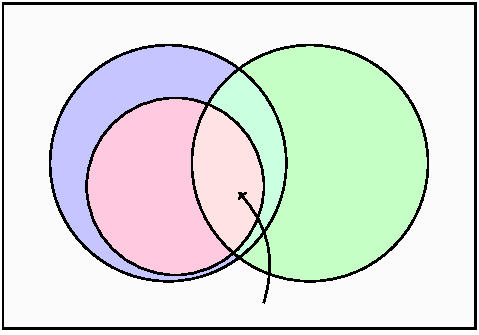
\includegraphics[width=.70\linewidth]{figures/coordinate-ring-venn-geometry.pdf}};
  \begin{scope}[x={(venn.south east)},y={(venn.north west)},every node/.style={font=\small,inner sep=0pt,align=center}]
    \node at (.50,.922) {环};
    \node at (.334,.762) {$K$-代数};
    \node at (.683,.740) {既约环};
    \node at (.327,.390) {有限生成的\\$K$-代数};
    \node at (.551,.061) {坐标环};
  \end{scope}
\end{tikzpicture}\par}
\smallskip

现在我们有了一套代数语言, 可以用来刻画和讨论坐标环. 下一章的目标是研究坐标环 $K[X]$ 能告诉我们有关仿射簇 $X$ 的哪些信息. 正如我们将看到的, 坐标环本质上知道与其对应的仿射簇的一切. 这一有力的事实使我们能够把环和 $K$-代数的所有代数工具用到仿射簇的研究中.

\BookExerciseHeading
\begin{BookExercises}
  \item\label{ex:subring-of-reduced-ring-is-reduced} 说明为什么既约环的任意子环都是既约的.
  \item\label{ex:prove-quotient-reduced-iff-ideal-radical} 证明 Proposition~\ref{prop:quotient-reduced-iff-ideal-radical}.
  \item\label{ex:direct-sums-and-reducedness}
    \begin{enumerate}[label=(\alph*)]
      \item 证明如果 $R$ 或 $S$ 是既约的, 则直和 $R\oplus S$ 是既约的. (回顾一下, 直和中的加法和乘法按分量定义.)
      \item 证明 $K$-代数 $A=K[x]/\langle x^{2}\rangle$ 与 $K\oplus K$ 作为 $K$-向量空间同构, 但作为环不同构.
    \end{enumerate}
  \item\label{ex:polynomial-rings-over-reduced-rings} 设 $R$ 是既约环. 证明 $R[x]$ 是既约的, 并用归纳法得出对任意 $n$, $R[x_{1},\ldots,x_{n}]$ 都是既约的.
  \item\label{ex:find-variety-of-subalgebra-square-cube} 设 $A=K[u^{2},u^{3}]\subseteq K[u]$.
    \begin{enumerate}[label=(\alph*)]
      \item 说明怎样知道 $A$ 是有限生成且既约的.
      \item 找出一个仿射簇 $X$, 使 $K[X]\cong A$, 并证明你的答案.
    \end{enumerate}
  \item\label{ex:find-affine-variety-of-linear-generators} 设 $A=K[u+w,v+w]\subseteq K[u,v,w]$. 找出一个仿射簇 $X$, 使 $K[X]\cong A$, 并证明你的答案.
  \item\label{ex:find-affine-variety-from-multiplication-table} 设 $A$ 是以
    \[
      \{x^{i}\mid i\geq0\}\cup\{x^{i}y\mid i\geq0\}
    \]
    为基的 $K$-向量空间. 在这些基元素上定义一个 (交换的) 乘积, 令
    \[
      \begin{aligned}
        x^{i}\cdot x^{j}&=x^{i+j},\\
        x^{i}\cdot x^{j}y&=x^{i+j}y,\qquad\text{并且}\\
        x^{i}y\cdot x^{j}y&=x^{i+j+3},
      \end{aligned}
    \]
    再以 $K$-线性的方式把这个乘积扩张到 $A$ 的所有元素.
    \begin{enumerate}[label=(\alph*)]
      \item 证明 $A$ 是有限生成的既约 $K$-代数.
      \item 找出一个仿射簇 $X$, 使 $K[X]\cong A$, 并证明你的答案.
    \end{enumerate}
  \item\label{ex:coordinate-ring-from-ideal-of-relations} 设 $a_{1},\ldots,a_{m}\in K[x_{1},\ldots,x_{n}]$, 考虑子代数
    \[
      A=K[a_{1},\ldots,a_{m}]\subseteq K[x_{1},\ldots,x_{n}].
    \]
    设 $I\subseteq K[y_{1},\ldots,y_{m}]$ 是 $a_{1},\ldots,a_{m}$ 的关系理想:
    \[
      f\in I\quad\Longleftrightarrow\quad
        f(a_{1},\ldots,a_{m})=0\in K[x_{1},\ldots,x_{n}].
    \]
    定义 $X=\mathcal{V}(I)\subseteq\mathbb{A}^{m}$. 证明 $K[X]\cong A$.
  \item\label{ex:examples-for-coordinate-ring-venn-regions} 对本节末尾\hyperref[fig:coordinate-rings-venn-diagram]{Venn 图}的每个区域, 各举一个属于该区域的环的明确例子.
\end{BookExercises}

\par\smallskip
{\footnotesize
\noindent\textbf{开放获取.} 本章按照
\href{http://creativecommons.org/licenses/by-nc/4.0/}{Creative Commons Attribution-NonCommercial 4.0 International License}
的条款授权. 该许可允许以任何媒介或格式进行非商业性使用, 分享, 改编, 分发和复制, 但须对原作者和来源作适当署名, 提供 Creative Commons 许可的链接, 并说明是否作了修改.

\noindent
\begin{minipage}[t]{.17\linewidth}
  \vspace{0pt}
\includegraphics[width=.9\linewidth]{figures/source-cc-by-nc.png}
\end{minipage}\hfill
\begin{minipage}[t]{.81\linewidth}
  \vspace{0pt}本章的图片或其他第三方材料均纳入本章的 Creative Commons 许可, 除非材料的署名行另有注明. 如果材料未纳入本章的 Creative Commons 许可, 且您拟进行的使用未获法律规定的许可或超出允许使用的范围, 则须直接向著作权持有人取得许可.
\end{minipage}\par}


\chapter{多项式映射}\label{chap:polynomial-maps}

\noindent\textbf{第 \thechapter{} 章学习目标}
\begin{itemize}
  \item 定义仿射簇之间的多项式映射并举例, 包括同构的例子.
  \item 定义与多项式映射关联的拉回同态, 并在具体例子中计算它.
  \item 利用拉回的双射性证明: 仿射簇同构当且仅当它们的坐标环同构.
  \item 描述代数与几何的等价, 以及它怎样在 $K$-代数和仿射簇的内在性质之间进行转换.
\end{itemize}

上一章给出了一个对应
\[
  \begin{aligned}
    \{\text{仿射簇}\}&\to\{\text{有限生成的既约 }K\text{-代数}\}\\
    X&\mapsto K[X]
  \end{aligned}
\]
并确认了它是满射. 但它是单射吗? 也就是说, 如果 $K[X]=K[Y]$, 是否必有 $X=Y$?

这个问题比乍看起来更微妙. 要回答它, 必须准确决定何时两个 $K$-代数是\textquotedbl{}同一个\textquotedbl{}: 例如, $K[x]$ 与 $K[y]$ 是同一个吗? 从字面上说, 不是. 但我们是如此习惯于把同构的环看成相同的, 所以读者觉得这个答案不能令人满意, 也是可以理解的. 为抓住同构就是\textquotedbl{}相同\textquotedbl{}这一直觉, 可以重新表述问题: 如果 $K[X]\cong K[Y]$, 是否必有 $X\cong Y$?

要处理这个问题, 必须首先精确定义两个仿射簇\textquotedbl{}同构\textquotedbl{}是什么意思, 从仿射簇之间保持结构的\textquotedbl{}态射\textquotedbl{}这一概念着手. 每当引入一种新类型的数学对象 (例如群, 环, 拓扑空间) 时, 都应做这件事: 问这些对象之间哪些映射保持有关的结构. 对群来说, 有关的映射是群同态; 对环来说, 是环同态; 对拓扑空间来说, 是连续映射. 因为代数几何研究多项式, 仿射簇之间有关的映射是多项式映射, 或许不足为奇. 我们将在本章引入这些映射.

有了多项式映射的定义, 就能说清仿射簇 $X$ 与 $Y$ 同构是什么意思, 并能证明 $X\cong Y$ 当且仅当 $K[X]\cong K[Y]$. 这一陈述称为\textquotedbl{}代数与几何的等价\textquotedbl{}, 是本章的目标, 也是代数与几何之间的词典的核心.

\par\smallskip
{\footnotesize
\noindent\textcopyright{} The Author(s) 2025\par
\noindent E. Clader, D. Ross, \emph{Beginning in Algebraic Geometry}, Undergraduate Texts in Mathematics,
\href{https://doi.org/10.1007/978-3-031-88819-9_5}{\nolinkurl{https://doi.org/10.1007/978-3-031-88819-9_5}}.\par}

\section{仿射簇之间的多项式映射}\label{sec:polynomial-maps-between-affine-varieties}

上一章介绍了仿射簇 $X\subseteq\mathbb{A}^{m}$ 的坐标环 $K[X]$, 其元素是多项式函数 $F:X\to K$. 把 $K$ 与 $\mathbb{A}^{1}$ 等同, 就可以把这类函数看成仿射簇之间的映射的特例 (即 $X$ 到 $\mathbb{A}^{1}$ 的映射). 我们的第一个目标是扩充这一定义, 使它涵盖从任意仿射簇到另一个仿射簇的映射.

\BookPairedNoteLeft
  {这里有意区分\textquotedbl{}函数\textquotedbl{}和\textquotedbl{}映射\textquotedbl{}两个词. 函数在基域中取值, 而映射在仿射簇中取值.}
  {设 $X\subseteq\mathbb{A}^{m}$ 是仿射簇. 因为坐标环 $K[X]$ 的每个元素都是函数 $X\to K$, 所以 $n$ 个元素 $F_{1},\ldots,F_{n}\in K[X]$ 给出一个映射 $X\to\mathbb{A}^{n}$, 定义为 $a\in X\mapsto(F_{1}(a),\ldots,F_{n}(a))\in\mathbb{A}^{n}$.}
\noindent 若 $Y\subseteq\mathbb{A}^{n}$ 为仿射簇, 且映射 $X\to\mathbb{A}^{n}$ 的像恰好落在 $Y$ 中, 就得到映射 $X\to Y$. 这样由多项式函数给出的映射称为多项式映射.

\begin{Definition}{仿射簇之间的多项式映射}\leavevmode\label{def:polynomial-map-between-affine-varieties}
  设 $X\subseteq\mathbb{A}^{m}$ 与 $Y\subseteq\mathbb{A}^{n}$ 为仿射簇. 若存在 $F_{1},\ldots,F_{n}\in K[X]$, 使得对每个 $a\in X$ 都有
  \[
    F(a)=(F_{1}(a),\ldots,F_{n}(a)),
  \]
  则称映射 $F:X\to Y$ 是\textbf{多项式映射}.
\end{Definition}

特别地, $X$ 上的多项式函数与多项式映射 $F:X\to\mathbb{A}^{1}$ 是完全相同的概念. 在下一例中, 我们考虑一个陪域是仿射空间 $\mathbb{A}^{3}$ 的多项式映射.

\begin{Example}{到仿射空间的多项式映射}\leavevmode\label{ex:polynomial-map-to-affine-space}
  考虑抛物线 $X=\mathcal{V}(x_{2}-x_{1}^{2})\subseteq\mathbb{A}^{2}$. (为给下一例作准备, 这里将变量记为 $x_{1},x_{2}$, 而不是 $x,y$.) 那么
  \[
    \begin{aligned}
      F:X&\to\mathbb{A}^{3}\\
      (a_{1},a_{2})&\mapsto(a_{1}-a_{1}^{2},a_{1}+a_{2},a_{1}^{2}-a_{2}^{2})
    \end{aligned}
  \]
  是多项式映射, 因为它的三个分量函数
  \[
    F_{1}(a_{1},a_{2})=a_{1}-a_{1}^{2},\quad F_{2}(a_{1},a_{2})=a_{1}+a_{2},
    \quad\text{以及}\quad F_{3}(a_{1},a_{2})=a_{1}^{2}-a_{2}^{2}
  \]
  分别来自多项式
  \[
    f_{1}=x_{1}-x_{1}^{2},\quad f_{2}=x_{1}+x_{2},\quad\text{以及}\quad f_{3}=x_{1}^{2}-x_{2}^{2},
  \]
  因而都是 $K[X]$ 的元素. 注意, 三个多项式
  \[
    g_{1}=x_{1}-x_{2},\quad g_{2}=x_{1}+x_{1}^{2},\quad\text{以及}\quad g_{3}=x_{2}-x_{2}^{2}
  \]
  给出同一个多项式映射 $F:X\to\mathbb{A}^{3}$, 因为 $[f_{i}]=[g_{i}]\in K[X]$.
\end{Example}

若 $X\subseteq\mathbb{A}^{m}$ 是仿射簇, 构造陪域为仿射空间的多项式映射 $F:X\to\mathbb{A}^{n}$ 并不困难. 具体来说, 任取多项式 $f_{1},\ldots,f_{n}\in K[x_{1},\ldots,x_{m}]$, 令
\[
  F_{i}=[f_{i}]\in\frac{K[x_{1},\ldots,x_{m}]}{\mathcal{I}(X)}=K[X],
\]
就定义了这种映射的坐标函数 $F_{1},\ldots,F_{n}$. 另一组选取的多项式 $g_{1},\ldots,g_{n}$ 给出同一个多项式映射, 当且仅当对每个 $i$ 都有 $f_{i}-g_{i}\in\mathcal{I}(X)$.

另一方面, 若 $Y\subsetneq\mathbb{A}^{n}$ 是不同于整个仿射空间的仿射簇, 那么并非每一组 $F_{1},\ldots,F_{n}\in K[X]$ 都给出映射 $F:X\to Y$. 特别地, 要保证 $X$ 中每个点的像都是 $Y$ 中的点, 必须要求对每个 $a\in X$, 点
\[
  (F_{1}(a),\ldots,F_{n}(a))\in\mathbb{A}^{n}
\]
确实落在 $Y$ 中, 即为 $Y$ 的定义多项式的零点. 更具体地, 若 $Y=\mathcal{V}(S)$, 其中 $S\subseteq K[x_{1},\ldots,x_{n}]$, 那么必须验证对每个 $a\in X$ 与每个 $g\in S$, 都有
\[
  g(F_{1}(a),\ldots,F_{n}(a))=0.
\]

\begin{Example}{到仿射簇的一个多项式映射}\leavevmode\label{ex:parabola-map-to-hyperbolic-paraboloid}
  \BookPairedFigure
    {和 Example~\ref{ex:polynomial-map-to-affine-space} 一样, 设 $X=\mathcal{V}(x_{2}-x_{1}^{2})\subseteq\mathbb{A}^{2}$, 但现在令 $Y=\mathcal{V}(y_{1}y_{2}-y_{3})\subseteq\mathbb{A}^{3}$. 在实数上, $Y$ 是\hyperref[fig:curve-on-hyperbolic-paraboloid]{右图}所示的双曲抛物面, 而 Example~\ref{ex:polynomial-map-to-affine-space} 中的函数
    \[
      \begin{aligned}
        F:X&\to Y\\
        (a_{1},a_{2})&\mapsto(a_{1}-a_{1}^{2},a_{1}+a_{2},a_{1}^{2}-a_{2}^{2})
      \end{aligned}
    \]
    是从 $X$ 到 $Y$ 的多项式映射, 它的像就是图中曲面上的那条曲线.}
    {\phantomsection\label{fig:curve-on-hyperbolic-paraboloid}%
      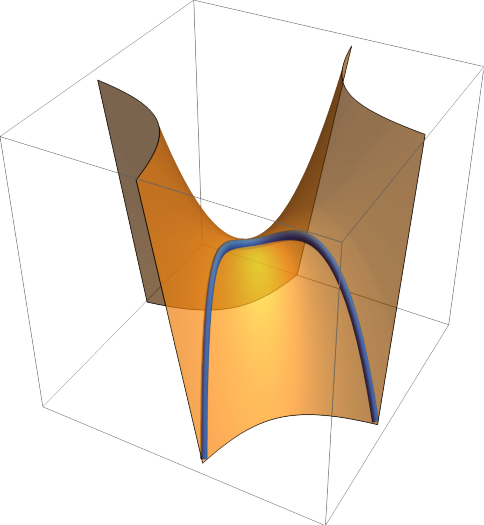
\includegraphics[width=\linewidth]{figures/curve-on-hyperbolic-paraboloid.png}}
  \noindent 我们已经验证 $F$ 的三个分量函数都是多项式函数, 但现在还必须确认其像确实落在 $Y$ 中. 这等价于断言 $F(a_{1},a_{2})$ 满足 $Y$ 的定义方程 $y_{1}y_{2}-y_{3}$, 换句话说, 只要 $(a_{1},a_{2})\in X$, 就有
  \[
    F_{1}(a_{1},a_{2})F_{2}(a_{1},a_{2})-F_{3}(a_{1},a_{2})=0.
  \]
  为验证这一点, 只需代入 $F_{1},F_{2},F_{3}$ 的表达式并整理:
  \[
    (a_{1}-a_{1}^{2})(a_{1}+a_{2})-(a_{1}^{2}-a_{2}^{2})
       =(a_{1}+a_{2})(a_{2}-a_{1}^{2})=(a_{1}+a_{2})\cdot0=0,
  \]
  其中第二个等号来自 $(a_{1},a_{2})\in X$, 它蕴含 $a_{2}-a_{1}^{2}=0$.
\end{Example}

\BookPairedNoteLeft
  {为区分 $X$ 与 $Y$ 上的坐标, 常像上一例那样使用下标: 对 $X$ 用 $x_{1},x_{2},\ldots$, 对 $Y$ 用 $y_{1},y_{2},\ldots$.}
  {读者从代数中已经熟悉这样的概念: 某些同态是同构, 而同构的对象具有一切有关的共同性质. 例如, 同构的群具有相同的群论性质.}
\noindent 类似地, 仿射簇的同构使我们能够讨论仿射簇在本质上相同是什么意思.

\begin{Definition}{仿射簇的同构}\leavevmode\label{def:isomorphism-of-affine-varieties}
  设 $X\subseteq\mathbb{A}^{m}$ 与 $Y\subseteq\mathbb{A}^{n}$ 为仿射簇. 若多项式映射 $F:X\to Y$ 有一个同样为多项式映射的逆函数 $F^{-1}:Y\to X$, 则称 $F$ 是一个\textbf{同构}. 若存在这样的同构, 则称 $X$ 与 $Y$ \textbf{同构}, 记作 $X\cong Y$.
\end{Definition}

\begin{Example}{抛物线同构于 $\mathbb{A}^{1}$}\leavevmode\label{ex:parabola-isomorphic-to-affine-line}
  \BookPairedFigure
    {设 $X=\mathcal{V}(x_{2}-x_{1}^{2})\subseteq\mathbb{A}^{2}$. 注意, 由下式定义的两个映射 $F$ 与 $G$
    \[
      \begin{aligned}
        F:X&\to\mathbb{A}^{1}&G:\mathbb{A}^{1}&\to X\\
        (a_{1},a_{2})&\mapsto a_{1}&b&\mapsto(b,b^{2})
      \end{aligned}
    \]
    都是多项式映射.}
    {\phantomsection\label{fig:parabola-isomorphism}%
      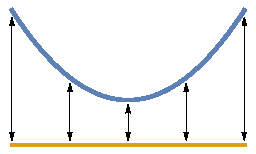
\includegraphics[width=\linewidth]{figures/parabola-isomorphism.pdf}}
  \noindent 此外, 容易验证 $F\circ G$ 是 $\mathbb{A}^{1}$ 上的恒等映射. 利用对每个 $(a_{1},a_{2})\in X$ 都有 $a_{2}=a_{1}^{2}$, 也可以验证 $G\circ F$ 是 $X$ 上的恒等映射. 因而 $X\cong\mathbb{A}^{1}$. \hyperref[fig:parabola-isomorphism]{上图}画出了 $\mathbb{R}$ 上仿射直线与抛物线之间的同构, 其中 $F$ 是向下的映射, $G$ 是向上的映射.
\end{Example}

\begin{Example}{给出同构的投影}\leavevmode\label{ex:isomorphic-projections}
  推广上一例, 假设 $X=\mathcal{V}(x_{m}-g)\subseteq\mathbb{A}^{m}$, 其中 $g\in K[x_{1},\ldots,x_{m-1}]$. 考虑两个映射
  \[
    \begin{aligned}
      F:X&\to\mathbb{A}^{m-1}\\
      (a_{1},\ldots,a_{m})&\mapsto(a_{1},\ldots,a_{m-1})
    \end{aligned}
  \]
  以及
  \[
    \begin{aligned}
      G:\mathbb{A}^{m-1}&\to X\\
      (b_{1},\ldots,b_{m-1})&\mapsto(b_{1},\ldots,b_{m-1},g(b_{1},\ldots,b_{m-1})).
    \end{aligned}
  \]
  $F$ 与 $G$ 都是多项式映射. 利用对每个 $(a_{1},\ldots,a_{m})\in X$ 都有 $a_{m}=g(a_{1},\ldots,a_{m-1})$, 可见两者互为逆映射. 因而 $X\cong\mathbb{A}^{m-1}$. 本例的进一步推广见 Exercise~\ref{ex:eliminate-a-linear-coordinate}.
\end{Example}

\begin{Example}{平移是同构}\leavevmode\label{ex:translation-is-iso}
  给定参考点 $c=(c_{1},\ldots,c_{m})\in\mathbb{A}^{m}$, 考虑平移映射
  \[
    \begin{aligned}
      T_{c}:\mathbb{A}^{m}&\to\mathbb{A}^{m}\\
      (a_{1},\ldots,a_{m})&\mapsto(a_{1}+c_{1},\ldots,a_{m}+c_{m}).
    \end{aligned}
  \]
  那么对任意仿射簇 $X\subseteq\mathbb{A}^{m}$, 平移 $T_{c}(X)$ 也是仿射簇. 为见此点, 注意多项式 $f(x_{1},\ldots,x_{m})$ 在 $T_{c}(X)$ 上处处为零, 当且仅当 $f(x_{1}+c_{1},\ldots,x_{m}+c_{m})$ 在 $X$ 上处处为零, 所以
  \[
    T_{c}(X)=\mathcal{V}\bigl(\{f\in K[x_{1},\ldots,x_{n}]
      \mid f(x_{1}+c_{1},\ldots,x_{m}+c_{m})\in\mathcal{I}(X)\}\bigr).
  \]
  映射 $T_{c}:X\to T_{c}(X)$ 显然是多项式映射, 而且实际上还是同构. 为证明这一点, 只需注意它有一个多项式逆映射, 即用参考点 $(-c_{1},\ldots,-c_{m})\in\mathbb{A}^{m}$ 作反向平移.

  Exercise~\ref{ex:invertible-affine-linear-map} 把本例推广到平移和可逆线性映射的复合; 这样的复合称为\textbf{仿射线性变换}.
\end{Example}

\BookPairedNote
  {仿射簇的映射要成为同构, 就必须是双射, 因为这是逆函数存在的必要条件. 然而, \emph{并非每个双射的仿射簇多项式映射都是同构}, 因为逆函数即使存在也未必是多项式映射.}
  {几何和代数在这里有所不同: 在代数中, 若同态 (群, 环, 代数等的同态) 有逆函数, 那么这个逆函数自动是同态. 见 Exercise~\ref{ex:bijective-k-algebra-homomorphism-is-isomorphism}.}
\noindent 下一例说明这一现象.

\begin{Example}{双射的多项式映射未必是同构}\leavevmode\label{ex:cusp-bijective-map-not-isomorphism}
  \BookPairedFigure
    {考虑 $X=\mathcal{V}(x^{2}-y^{3})\subseteq\mathbb{A}^{2}$. 那么
    \[
      \begin{aligned}
        F:\mathbb{A}^{1}&\to X\\
        a&\mapsto(a^{3},a^{2})
      \end{aligned}
    \]
    是\hyperref[fig:cusp-polynomial-map]{右图}所示的多项式映射. (注意, 对每个 $a\in\mathbb{A}^{1}$, 点 $(a^{3},a^{2})\in\mathbb{A}^{2}$ 确实满足方程 $x^{2}-y^{3}=0$.)}
    {\phantomsection\label{fig:cusp-polynomial-map}%
      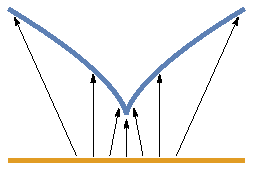
\includegraphics[width=\linewidth]{figures/cusp-polynomial-map.pdf}}
  \noindent 此外, 读者可以验证 $F$ 的一个逆函数为
  \[
    \begin{aligned}
      G:X&\to\mathbb{A}^{1}\\
      (b,c)&\mapsto
       \begin{cases}
         b/c & \text{若 }c\ne0,\\
         0   & \text{若 }c=0.
       \end{cases}
    \end{aligned}
  \]
  然而, $G$ 不是多项式映射. $G$ 涉及对输入作除法, 这的确暗示它可能不是多项式映射. 但如 Example~\ref{ex:apparently-nonpolynomial-hyperbola-function} 所示, 要确定 $G$ 不是多项式映射, 仍需更加谨慎. 下一节将建立证明 $X\not\cong\mathbb{A}^{1}$ 所需的工具, 由此可知 $G$ 不可能是多项式映射. 曲线 $X$ 似乎改变方向的\textquotedbl{}尖点\textquotedbl{}给出了 $X\not\cong\mathbb{A}^{1}$ 的一个直观线索.
\end{Example}

要证明 $X\cong Y$, 做法相对直接: 必须找到 $X$ 与 $Y$ 之间的一个同构. 但证明 $X\not\cong Y$ 更微妙. 怎样严格证明不存在任何同构? 在代数中, 我们有不少工具做这件事: 要证明两个环不同构, 可以找到某种一个环具有而另一个不具有的环论性质, 例如是整环或者是 UFD.

因此, 如果想要判定何时两个仿射簇不同构, 一个自然的办法是证明 $X\cong Y$ 蕴含 $K[X]\cong K[Y]$. 一旦做到这一点, 证明 $K[X]\not\cong K[Y]$ 的代数论证就会蕴含几何结论 $X\not\cong Y$, 于是可以用代数方法判定何时仿射簇不同构. 因而, 我们的目标是建立一个过程, 将仿射簇的同构转换成对应坐标环的同构. 这个过程就是拉回, 是下一节的主题.

\BookExerciseHeading
\begin{BookExercises}
  \item\label{ex:polynomial-map-to-two-equation-variety} 设 $X=\mathcal{V}(y^{2}-z^{2}+xy-z,z^{2}-x^{3}y^{2})\subseteq\mathbb{A}^{3}$. 证明 $F(a)=(1,a,a)$ 定义了多项式映射 $F:\mathbb{A}^{1}\to X$. $F$ 是同构吗?
  \item\label{ex:polynomial-map-between-two-circles} 设 $X=\mathcal{V}(x^{2}+y^{2}-1)\subseteq\mathbb{A}^{2}$, 并设 $Y=\mathcal{V}(u^{2}+v^{2}-2)\subseteq\mathbb{A}^{2}$. 证明 $F(a,b)=(a+b,a-b)$ 定义了多项式映射 $F:X\to Y$. $F$ 是同构吗?
  \item\label{ex:polynomial-map-to-nodal-cubic} 设 $X=\mathcal{V}(y^{2}-x^{3}-x^{2})\subseteq\mathbb{A}^{2}$. 证明 $F(a)=(a^{2}-1,a^{3}-a)$ 定义了多项式映射 $F:\mathbb{A}^{1}\to X$. $F$ 是同构吗? (提示: 画图.)
  \item\label{ex:eliminate-a-linear-coordinate} 设 $X=\mathcal{V}(f_{1},\ldots,f_{k},x_{m}-g)\subseteq\mathbb{A}^{m}$, 其中 $g\in K[x_{1},\ldots,x_{m-1}]$, $f_{1},\ldots,f_{k}\in K[x_{1},\ldots,x_{m}]$. 对每个 $i=1,\ldots,k$, 定义
    \[
      \widetilde{f}_{i}=f_{i}(x_{1},\ldots,x_{m-1},g)\in K[x_{1},\ldots,x_{m-1}],
    \]
    并令 $Y=\mathcal{V}(\widetilde{f}_{1},\ldots,\widetilde{f}_{k})\subseteq\mathbb{A}^{m-1}$. 证明 $X\cong Y$. (这说明如果一个仿射簇的某个定义方程对其中一个变量是线性的, 那么就可以用一个与之同构的仿射簇取代它, 新簇由更少变量中的更少方程定义.)
  \item\label{ex:polynomial-image-may-not-be-variety}
    \begin{enumerate}[label=(\alph*)]
      \item 证明多项式映射
        \[
          \begin{aligned}
            F:\mathbb{A}^{1}&\to\mathbb{A}^{3}\\
            a&\mapsto(a,a^{2},a^{3})
          \end{aligned}
        \]
        的像是仿射簇.
      \item 证明多项式映射
        \[
          \begin{aligned}
            G:\mathbb{A}^{2}&\to\mathbb{A}^{2}\\
            (a,b)&\mapsto(a,ab)
          \end{aligned}
        \]
        的像不是仿射簇.
    \end{enumerate}
    因此, 多项式映射的像可能是仿射簇, 也可能不是.
  \item\label{ex:invertible-affine-linear-map} 设 $M$ 是一个系数在 $K$ 中的可逆 $m\times m$ 矩阵, 且 $c\in\mathbb{A}^{m}$. 将 $\mathbb{A}^{m}$ 与向量空间 $K^{m}$ 等同, 并将 $M$ 与线性变换 $\phi_{M}:K^{m}\to K^{m}$ 等同, 定义函数
    \[
      \begin{aligned}
        F:\mathbb{A}^{m}&\to\mathbb{A}^{m}\\
        a&\mapsto\phi_{M}(a)+c.
      \end{aligned}
    \]
    证明下列结论.
    \begin{enumerate}[label=(\alph*)]
      \item 若 $X\subseteq\mathbb{A}^{m}$ 是仿射簇, 则 $F(X)\subseteq\mathbb{A}^{m}$ 是仿射簇.
      \item 若 $X\subseteq\mathbb{A}^{m}$ 是仿射簇, 则 $X\cong F(X)$.
    \end{enumerate}
  \item\label{ex:linear-equations-give-affine-space} 设 $X=\mathcal{V}(\ell_{1},\ldots,\ell_{k})\subseteq\mathbb{A}^{n}$, 其中每个 $\ell_{i}$ 都是线性多项式:
    \[
      \ell_{i}=a_{i1}x_{1}+\cdots+a_{in}x_{n}+b_{i}\in K[x_{1},\ldots,x_{n}].
    \]
    令 $M=(a_{ij})$ 为 $k\times n$ 的系数矩阵. 假设 $X$ 非空, 证明
    \[
      X\cong\mathbb{A}^{n-\operatorname{rk}(M)}.
    \]
    (提示: 使用秩--零度定理.)
\end{BookExercises}

\par\smallskip
{\footnotesize
\noindent\textbf{开放获取.} 本章按照
\href{http://creativecommons.org/licenses/by-nc/4.0/}{Creative Commons Attribution-NonCommercial 4.0 International License}
的条款授权. 该许可允许以任何媒介或格式进行非商业性使用, 分享, 改编, 分发和复制, 但须对原作者和来源作适当署名, 提供 Creative Commons 许可的链接, 并说明是否作了修改.

\noindent
\begin{minipage}[t]{.17\linewidth}
  \vspace{0pt}
\includegraphics[width=.9\linewidth]{figures/source-cc-by-nc.png}
\end{minipage}\hfill
\begin{minipage}[t]{.81\linewidth}
  \vspace{0pt}本章的图片或其他第三方材料均纳入本章的 Creative Commons 许可, 除非材料的署名行另有注明. 如果材料未纳入本章的 Creative Commons 许可, 且您拟进行的使用未获法律规定的许可或超出允许使用的范围, 则须直接向著作权持有人取得许可.
\end{minipage}\par}

\section{拉回同态}\label{sec:pullback-homomorphisms}

\BookPairedNote
  {多项式映射是仿射簇之间保持结构的映射, 正如同态是代数对象之间保持结构的映射. 就像能在对象层面从几何走向代数, 即把 $X$ 送到 $K[X]$, 也能在映射层面从几何走向代数.}
  {粗略地说, 一族数学对象及其之间保持结构的映射, 就构成了一个\textquotedbl{}范畴\textquotedbl{}.}
\noindent 具体来说, 可以把仿射簇之间的多项式映射送到坐标环之间相应的 $K$-代数同态. 映射层面的这一转换由拉回同态给出.

\begin{Definition}{拉回同态}\leavevmode\label{def:pullback-homomorphism}
  设 $X\subseteq\mathbb{A}^{m}$ 和 $Y\subseteq\mathbb{A}^{n}$ 为仿射簇, $F:X\to Y$ 为多项式映射. $F$ 诱导的\textbf{拉回同态}为
  \[
    \begin{aligned}
      F^{*}: K[Y]&\to K[X]\\
      F^{*}(G)&=G\circ F.
    \end{aligned}
  \]
\end{Definition}

\BookPairedNoteLeft
  {注意, 拉回改变了映射方向:
   \[
     F:X\to Y\ \Longrightarrow\ F^{*}:K[Y]\to K[X].
   \]}
  {为了使拉回同态的定义有意义, 必须验证对每个 $G\in K[Y]$, 复合 $G\circ F$ 都是 $K[X]$ 的元素. 由于 $G:Y\to K$ 且 $F:X\to Y$, 根据复合的定义, $G\circ F$ 确实是一个从 $X$ 到 $K$ 的函数.}
\noindent 示意如下:
\[
  X\xrightarrow{F}Y\xrightarrow{G}K\ \Longrightarrow\ X\xrightarrow{G\circ F}K.
\]
进一步, $G\circ F$ 是多项式函数, 这是因为多项式函数的复合仍是多项式函数 (Exercise~\ref{ex:composing-with-polynomial-map}).

\begin{Example}{拉回同态}\leavevmode\label{ex:pullback-homomorphism-calculation}
  设 $X=\mathcal{V}(x_{2}-x_{1}^{2})\subseteq\mathbb{A}^{2}$, $Y=\mathcal{V}(y_{1}y_{2}-y_{3})\subseteq\mathbb{A}^{3}$. 回顾 Example~\ref{ex:parabola-map-to-hyperbolic-paraboloid} 中的多项式映射 $F:X\to Y$:
  \[
    F(a_{1},a_{2})=(a_{1}-a_{1}^{2},a_{1}+a_{2},a_{1}^{2}-a_{2}^{2}).
  \]
  考虑由 $G(b_{1},b_{2},b_{3})=b_{1}^{2}-b_{2}b_{3}$ 定义的函数 $G\in K[Y]$. 沿 $F$ 拉回, 得到多项式函数 $F^{*}(G)\in K[X]$, 定义为
  \[
    (F^{*}G)(a_{1},a_{2})=(G\circ F)(a_{1},a_{2})=(a_{1}-a_{1}^{2})^{2}-(a_{1}+a_{2})(a_{1}^{2}-a_{2}^{2}).
  \]
  类似地, 将由 $H(b_{1},b_{2},b_{3})=b_{1}+b_{2}-b_{3}$ 定义的 $H\in K[Y]$ 拉回, 得到多项式函数 $F^{*}(H)\in K[X]$, 定义为
  \[
    (F^{*}H)(a_{1},a_{2})=(H\circ F)(a_{1},a_{2})=(a_{1}-a_{1}^{2})+(a_{1}+a_{2})-(a_{1}^{2}-a_{2}^{2}).
  \]
\end{Example}

如上一例所示, 选定 $F=(F_{1},\ldots,F_{n})$ 和 $G$ 的多项式表达式后, 只需将 $F$ 和 $G$ 的多项式表达式复合, 就得到 $F^{*}(G)$ 的多项式表达式. 将这一观察展开, 设 $X\subseteq\mathbb{A}^{m}$ 和 $Y\subseteq\mathbb{A}^{n}$. 则
\[
  K[X]=\frac{K[x_{1},\ldots,x_{m}]}{\mathcal{I}(X)}
  \qquad\text{且}\qquad
  K[Y]=\frac{K[y_{1},\ldots,y_{n}]}{\mathcal{I}(Y)}.
\]
若选取多项式 $f_{1},\ldots,f_{n}\in K[x_{1},\ldots,x_{m}]$ 和 $g\in K[y_{1},\ldots,y_{n}]$, 使 $F_{i}=[f_{i}]$ 且 $G=[g]$, 则对每个 $a\in X$ 和 $b=(b_{1},\ldots,b_{n})\in Y$, 有
\[
  F(a)=(f_{1}(a),\ldots,f_{n}(a))
  \qquad\text{且}\qquad
  G(b_{1},\ldots,b_{n})=g(b_{1},\ldots,b_{n}).
\]
这蕴含
\[
  F^{*}(G)(a)=G(F(a))=g(f_{1}(a),\ldots,f_{n}(a)).
\]
因此 $F^{*}(G)=[g(f_{1},\ldots,f_{n})]$, 其中 $g(f_{1},\ldots,f_{n})\in K[x_{1},\ldots,x_{m}]$ 是将 $g$ 中的 $y_{i}$ 替换成 $f_{i}(x_{1},\ldots,x_{m})$ 所得的多项式.

\begin{Example}{再看拉回同态}\leavevmode\label{ex:pullback-by-polynomial-substitution}
  在 Example~\ref{ex:pullback-homomorphism-calculation} 的同一情形中, $F$ 的各分量函数来自多项式
  \[
    f_{1}(x_{1},x_{2})=x_{1}-x_{1}^{2},\quad f_{2}(x_{1},x_{2})=x_{1}+x_{2},\quad
    \text{以及}\quad f_{3}(x_{1},x_{2})=x_{1}^{2}-x_{2}^{2}.
  \]
  多项式函数 $G\in K[Y]$ 来自多项式
  \[
    g=y_{1}^{2}-y_{2}y_{3}.
  \]
  直接观察便可看出, 拉回函数 $F^{*}(G)$ 来自多项式
  \[
    g(f_{1},f_{2},f_{3})=(x_{1}-x_{1}^{2})^{2}-(x_{1}+x_{2})(x_{1}^{2}-x_{2}^{2}).
  \]
\end{Example}

顾名思义, 拉回同态不只是一个函数, 还是 $K$-代数同态. 下面验证这一点.

\begin{Proposition}{$F^{*}$ 是同态}\leavevmode\label{prop:pullback-is-homomorphism}
  若 $X\subseteq\mathbb{A}^{m}$ 和 $Y\subseteq\mathbb{A}^{n}$ 为仿射簇, $F:X\to Y$ 为多项式映射, 则
  \[
    F^{*}:K[Y]\to K[X]
  \]
  是 $K$-代数同态.
\end{Proposition}

\begin{Proof}
\BookPairedNote
  {要证明 $F^{*}$ 是 $K$-代数同态, 必须验证它保持加法, 乘法和数乘. 我们正式证明第一个性质, 把其余两个留给 Exercise~\ref{ex:pullback-preserves-multiplications}.}
  {有高等线性代数基础的读者也许会看出, 拉回同态是线性映射的对偶映射的推广; 见 Exercise~\ref{ex:pullback-restricts-to-dual-map}.}
\noindent 为说明 $F^{*}$ 保持加法, 设 $G_{1},G_{2}\in K[Y]$ 为两个多项式函数. 在任意 $a\in X$ 处对 $F^{*}(G_{1}+G_{2})$ 求值, 得到
\[
  \begin{aligned}
    \bigl(F^{*}(G_{1}+G_{2})\bigr)(a)&=\bigl((G_{1}+G_{2})\circ F\bigr)(a)
       &&\text{(拉回的定义)}\\
    &=(G_{1}+G_{2})(F(a)) &&\text{(复合的定义)}\\
    &=G_{1}(F(a))+G_{2}(F(a)) &&\text{($K[Y]$ 中 $+$ 的定义)}\\
    &=(G_{1}\circ F)(a)+(G_{2}\circ F)(a) &&\text{(复合的定义)}\\
    &=\bigl((G_{1}\circ F)+(G_{2}\circ F)\bigr)(a) &&\text{($K[X]$ 中 $+$ 的定义)}\\
    &=(F^{*}G_{1}+F^{*}G_{2})(a) &&\text{(拉回的定义)}.
  \end{aligned}
\]
所以 $F^{*}(G_{1}+G_{2})=F^{*}G_{1}+F^{*}G_{2}$, 这就验证了 $F^{*}$ 保持加法.
\end{Proof}

回顾一下, 我们引入拉回同态, 是为了取得判定两个仿射簇是否同构的代数工具. 由于在任何范畴中, \textquotedbl{}同构\textquotedbl{}的定义都要求验证两个态射的复合等于恒等映射, 为实现这一目标, 首先要证明拉回与复合及恒等函数相容.

\begin{Proposition}{拉回保持复合与恒等映射}\leavevmode\label{prop:pullback-preserves-compositions-and-identity}
  设 $X\subseteq\mathbb{A}^{\ell}$, $Y\subseteq\mathbb{A}^{m}$ 和 $Z\subseteq\mathbb{A}^{n}$ 为仿射簇.
  \begin{enumerate}
    \item 若 $F:X\to Y$ 和 $G:Y\to Z$ 为多项式映射, 则
      \[
        (G\circ F)^{*}=F^{*}\circ G^{*}.
      \]
    \item 恒等函数的拉回是恒等函数:
      \[
        (\operatorname{id}_{X})^{*}=\operatorname{id}_{K[X]}.
      \]
  \end{enumerate}
\end{Proposition}

\begin{Proof}
\BookPairedNote
  {为证明第一条, 设 $H\in K[Z]$. 利用复合的结合律, 计算如下.}
  {在范畴论中, 拉回的这些性质称为\textquotedbl{}函子性\textquotedbl{}.}
\[
  (G\circ F)^{*}(H)=H\circ(G\circ F)=(H\circ G)\circ F
    =F^{*}(H\circ G)=F^{*}(G^{*}(H)),
\]
这说明 $(G\circ F)^{*}=F^{*}\circ G^{*}$. 对于第二条, 设 $H\in K[X]$. 则
\[
  (\operatorname{id}_{X})^{*}(H)=H\circ\operatorname{id}_{X}=H,
\]
所以 $(\operatorname{id}_{X})^{*}$ 确实是 $K[X]$ 上的恒等函数.
\end{Proof}

现在可以实现用坐标环判定仿射簇是否同构的目标了.

\begin{Corollary}{同构的拉回仍是同构}\leavevmode\label{cor:pullback-of-isomorphism}
  设 $X\subseteq\mathbb{A}^{m}$ 和 $Y\subseteq\mathbb{A}^{n}$ 为仿射簇. 若 $F:X\to Y$ 是同构, 则 $F^{*}:K[Y]\to K[X]$ 是同构.
\end{Corollary}

\begin{Proof}
  设 $F:X\to Y$ 为同构, 其逆为 $F^{-1}:Y\to X$. 为证明 $F^{*}$ 是同构, 只需证明 $F^{*}$ 与 $(F^{-1})^{*}$ 互为逆映射. 利用 Proposition~\ref{prop:pullback-preserves-compositions-and-identity} 验证如下:
  \[
    F^{*}\circ(F^{-1})^{*}=(F^{-1}\circ F)^{*}=(\operatorname{id}_{X})^{*}=\operatorname{id}_{K[X]}
  \]
  以及
  \[
    (F^{-1})^{*}\circ F^{*}=(F\circ F^{-1})^{*}=(\operatorname{id}_{Y})^{*}=\operatorname{id}_{K[Y]}.
  \]
\end{Proof}

Corollary~\ref{cor:pullback-of-isomorphism} 的逆命题也成立, 但证明还需要一些工具, 因此留到下一节再讨论. 现在先看几个应用上述结果的例子.

\begin{Example}{$\mathcal{V}(xy)\not\cong\mathbb{A}^{1}$}\leavevmode\label{ex:crossing-lines-not-isomorphic-to-line}
  考虑仿射簇 $X=\mathcal{V}(xy)\subseteq\mathbb{A}^{2}$. 我们来证明 $X$ 不同构于 $\mathbb{A}^{1}$. 直观上, 从\hyperref[fig:crossing-lines-vs-line]{下图}画出的两个簇应当不难看出这一点. 具体来说, $X$ 由相交于一点的两条仿射直线组成, 看起来当然与一条仿射直线很不同.
  \par\smallskip
  {\centering\phantomsection\label{fig:crossing-lines-vs-line}%
  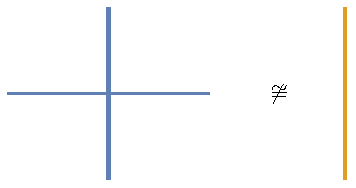
\includegraphics[width=.53\linewidth]{figures/crossing-lines-vs-line.pdf}\par}
  \smallskip
  为把这一直觉说准确, 注意 $X=\mathcal{V}(x)\cup\mathcal{V}(y)$ 是可约仿射簇. 因此 $\mathcal{I}(X)$ 不是素理想, 从而
  \[
    K[X]=\frac{K[x,y]}{\mathcal{I}(X)}
  \]
  不是整环. 由于 $K[\mathbb{A}^{1}]=K[z]$ 是一元多项式环, 它是整环. 因而, 由于同构保持\textquotedbl{}是整环\textquotedbl{}这一性质, 可知 $K[X]\not\cong K[\mathbb{A}^{1}]$, 由 Corollary~\ref{cor:pullback-of-isomorphism} 的逆否命题可得 $X\not\cong\mathbb{A}^{1}$.
\end{Example}

上一例很容易推广: 若一个仿射簇不可约而另一个可约, 则它们不可能同构, 因为其中一个的坐标环是整环, 而另一个的不是. 相比之下, 下一例说明怎样证明两个\emph{不可约}仿射簇不同构, 这可能更棘手. 这个例子还完成了我们在 Example~\ref{ex:cusp-bijective-map-not-isomorphism} 中开始的讨论, 即仿射簇之间的双射多项式映射不一定是同构.

\begin{Example}{$\mathcal{V}(x^{2}-y^{3})\not\cong\mathbb{A}^{1}$}\leavevmode\label{ex:cusp-not-isomorphic-to-line}
  与 Example~\ref{ex:cusp-bijective-map-not-isomorphism} 一样, 设 $X=\mathcal{V}(x^{2}-y^{3})\subseteq\mathbb{A}^{2}$. 为说明由 $f(a)=(a^{3},a^{2})$ 定义的多项式双射 $F:\mathbb{A}^{1}\to X$ 没有多项式逆映射, 我们证明 $X\not\cong\mathbb{A}^{1}$. 为此, 分析这两个簇的坐标环. 由于 $x^{2}-y^{3}$ 不可约, $X$ 的消没理想为
  \[
    \mathcal{I}(X)=\langle x^{2}-y^{3}\rangle.
  \]
  因此
  \[
    K[X]=\frac{K[x,y]}{\langle x^{2}-y^{3}\rangle}.
  \]
  要证明 $X\not\cong\mathbb{A}^{1}$, 只需找到一元多项式环 $K[\mathbb{A}^{1}]=K[z]$ 具有而 $K[X]$ 不具有的一个环论性质. 例如, $K[X]$ 不是 UFD. 实际上, 可以证明 (Exercise~\ref{ex:factorization-domain-not-unique}) $[x]$ 和 $[y]$ 是 $K[X]$ 中不同的不可约元, 所以等式
  \[
    [x]^{2}=[y]^{3}
  \]
  用两种不等价的方式把同一个元素表示成不可约元的乘积.
\end{Example}

本节讨论了怎样给每个多项式映射配上一个 $K$-代数同态. 具体来说, 我们得到一个从仿射簇范畴到 $K$-代数范畴的对应, 它在对象和态射上的定义分别为
\[
  \begin{aligned}
    X&\longmapsto K[X]\\
    (F:X\to Y)&\longmapsto(F^{*}:K[Y]\to K[X]).
  \end{aligned}
\]
连同 Proposition~\ref{prop:pullback-preserves-compositions-and-identity} 中的条件, 这样的对应称为这两个范畴之间的\textbf{函子}. 下一节将说明态射的对应是可逆的: 坐标环之间的每个 $K$-代数同态都来自相应仿射簇之间唯一的多项式映射. 这是证明 Corollary~\ref{cor:pullback-of-isomorphism} 的逆命题的关键一步, 我们将在 Corollary~\ref{cor:coordinate-rings-detect-isomorphisms} 中证明该逆命题.

\BookExerciseHeading
\begin{BookExercises}
  \item\label{ex:compute-pullback-quadratic} 设 $F:\mathbb{A}^{2}\to\mathbb{A}^{2}$ 为如下定义的多项式映射:
    \[
      F(a_{1},a_{2})=(a_{1}^{2}+2a_{1}a_{2},a_{1}-a_{2}).
    \]
    计算 $F^{*}(G)$, 其中 $G\in K[\mathbb{A}^{2}]$ 是由下式定义的函数:
    \[
      G(b_{1},b_{2})=b_{1}-b_{2}^{2}.
    \]
  \item\label{ex:compute-pullback-to-parametrized-line} 设 $Y=\mathcal{V}(y_{3}-y_{1}^{3})\subseteq\mathbb{A}^{3}$, $F:\mathbb{A}^{1}\to Y$ 为如下定义的多项式映射:
    \[
      F(a)=(a,a^{2},a^{3}).
    \]
    计算 $F^{*}([g])\in K[\mathbb{A}^{1}]$, 其中 $g=y_{1}y_{2}+y_{3}^{2}\in K[y_{1},y_{2},y_{3}]$.
  \item\label{ex:composing-with-polynomial-map} 设 $X$ 和 $Y$ 为仿射簇, $F:X\to Y$ 为函数. 证明: 若 $F$ 是多项式映射, 则对任意 $G\in K[Y]$, 有 $G\circ F\in K[X]$.
  \item\label{ex:converse-polynomial-composition} 设 $X$ 和 $Y$ 为仿射簇, $F:X\to Y$ 为函数. 证明: 若对所有 $G\in K[Y]$ 都有 $F\circ G\in K[X]$, 则 $F$ 是多项式映射. (这是上一题的逆命题.)
  \item\label{ex:pullback-of-inclusion} 设 $X,Y\subseteq\mathbb{A}^{n}$ 为仿射簇, $X\subseteq Y$, $F:X\to Y$ 为包含映射. 描述 $F^{*}:K[Y]\to K[X]$.
  \item\label{ex:pullback-preserves-multiplications} 设 $X$ 和 $Y$ 为仿射簇, $F:X\to Y$ 为多项式映射. 证明拉回 $F^{*}:K[Y]\to K[X]$ 保持环乘法和数乘.
  \item\label{ex:decide-variety-isomorphisms} 对下面的每对仿射簇 $X$ 和 $Y$, 判定是否有 $X\cong Y$, 并证明你的答案.
    \begin{enumerate}[label=(\alph*)]
      \item $X=\mathbb{A}^{1}$, $Y=\mathbb{A}^{2}$
      \item $X=\mathcal{V}(x_{1},x_{2})\subseteq\mathbb{A}^{2}$, $Y=\mathcal{V}(y_{1}-y_{2},y_{1}^{2}-y_{2})\subseteq\mathbb{A}^{2}$
      \item $X=\mathcal{V}(x_{3}-x_{1}^{2}+x_{1}x_{2})\subseteq\mathbb{A}^{3}$, $Y=\mathbb{A}^{2}$
      \item $X=\mathcal{V}(x_{1}x_{2})\subseteq\mathbb{A}^{2}$, $Y=\mathcal{V}(y_{1}^{2}-y_{2}^{2})\subseteq\mathbb{A}^{2}$
    \end{enumerate}
  \item\label{ex:hyperbola-not-isomorphic-to-line} 证明 $\mathcal{V}(xy-1)\subseteq\mathbb{A}^{2}$ 不同构于 $\mathbb{A}^{1}$.
  \item\label{ex:pullback-injectivity-and-surjectivity} 设 $X\subseteq\mathbb{A}^{m}$ 和 $Y\subseteq\mathbb{A}^{n}$ 为仿射簇, $F:X\to Y$ 为多项式映射.
    \begin{enumerate}[label=(\alph*)]
      \item 证明若 $F$ 是满射, 则 $F^{*}$ 是单射.
      \item 根据 (a), 我们或许会希望 $F$ 是单射时 $F^{*}$ 是满射. 证明这是错的, 方法是说明多项式映射
        \[
          \begin{aligned}
            F:\mathcal{V}(xy-1)&\to\mathbb{A}^{1}\\
            F(a,b)&=a
          \end{aligned}
        \]
        是单射, 但 $F^{*}$ 不是满射.
    \end{enumerate}
  \item\label{ex:density-dominance-and-injective-pullback}
    \begin{enumerate}[label=(\alph*)]
      \item 设 $Y\subseteq\mathbb{A}^{n}$ 为仿射簇, $X\subseteq Y$ 为子集. 若不存在仿射簇 $Z\subseteq\mathbb{A}^{n}$ 使 $X\subseteq Z\subsetneq Y$, 则称 $X$ 在 $Y$ 中稠密. 证明 $X$ 在 $Y$ 中稠密当且仅当 $K[Y]$ 中在 $X$ 上消没的唯一多项式函数 $G$ 是零函数.
      \item 设 $X\subseteq\mathbb{A}^{m}$ 和 $Y\subseteq\mathbb{A}^{n}$ 为仿射簇. 若 $F(X)$ 在 $Y$ 中稠密, 则称多项式映射 $F:X\to Y$ 是支配的. 证明多项式映射是支配的当且仅当它的拉回是单射.
    \end{enumerate}
  \item\label{ex:closed-embedding-surjective-pullback} 设 $X\subseteq\mathbb{A}^{m}$ 和 $Y\subseteq\mathbb{A}^{n}$ 为仿射簇. 若存在仿射簇 $Z\subseteq\mathbb{A}^{n}$, 使 $F(X)=Z$ 且诱导的映射 $F:X\to Z$ 是同构, 则称多项式映射 $F:X\to Y$ 是闭嵌入. 证明多项式映射是闭嵌入当且仅当它的拉回是满射.
  \item\label{ex:pullback-restricts-to-dual-map} (供学过一些高等线性代数的读者.) 设 $V,W$ 为 $K$-向量空间, $F:V\to W$ 为线性映射. 为 $V,W$ 选取基, 固定同构 $V\cong K^{m}$ 和 $W\cong K^{n}$; 通过这些同构, 可将 $V,W$ 分别等同于仿射空间 $\mathbb{A}^{m}_{K}$ 和 $\mathbb{A}^{n}_{K}$, 从而将它们视为仿射簇. 用 $V^{\vee},W^{\vee}$ 表示对偶向量空间, 说明为什么
    \[
      V^{\vee}\subseteq K[V]\qquad\text{且}\qquad W^{\vee}\subseteq K[W],
    \]
    并验证 $F^{*}|_{W^{\vee}}$ 与对偶映射 $F^{\vee}:W^{\vee}\to V^{\vee}$ 一致.
\end{BookExercises}

\section{拉回是双射}\label{sec:pullback-is-bijection}

若 $X\subseteq\mathbb{A}^{m}$ 和 $Y\subseteq\mathbb{A}^{n}$ 为仿射簇, 则把多项式映射送到其拉回的对应给出了两个态射集合之间的函数:
\[
  \begin{aligned}
    \{X\to Y\text{ 的多项式映射}\}
      &\to\{K[Y]\to K[X]\text{ 的 }K\text{-代数同态}\}\\
    F&\mapsto F^{*}.
  \end{aligned}
\]
本节的主要结论是这个函数为双射.

\begin{Proposition}{多项式函数的拉回给出双射}\leavevmode\label{prop:pullback-bijection}
  设 $X\subseteq\mathbb{A}^{m}$ 和 $Y\subseteq\mathbb{A}^{n}$ 为仿射簇. 对应 $F\mapsto F^{*}$ 是从多项式映射 $X\to Y$ 的集合到 $K$-代数同态 $K[Y]\to K[X]$ 的集合的双射.
\end{Proposition}

\BookPairedNoteLeft
  {用范畴论的语言来说, Proposition~\ref{prop:pullback-bijection} 所给的双射表明, 把 $X$ 送到 $K[X]$, 把 $F$ 送到 $F^{*}$ 的函子是\textquotedbl{}全忠实的\textquotedbl{}.}
  {为证明 Proposition~\ref{prop:pullback-bijection}, 只需构造把 $F$ 送到 $F^{*}$ 的过程的逆. 也就是说, 给定任意 $K$-代数同态 $\phi:K[Y]\to K[X]$, 只需说明存在唯一的多项式映射 $F:X\to Y$ 使 $F^{*}=\phi$.}
\noindent 这一结论的证明由于记号的缘故可能不易读懂, 因此先看一个具体例子. 建议读者在学习证明时回看这一例子.

\begin{Example}{由拉回恢复原映射}\leavevmode\label{ex:invert-pullback}
  考虑 Example~\ref{ex:parabola-map-to-hyperbolic-paraboloid} 中的仿射簇:
  \[
    X=\mathcal{V}(x_{2}-x_{1}^{2})\subseteq\mathbb{A}^{2}
    \qquad\text{且}\qquad
    Y=\mathcal{V}(y_{1}y_{2}-y_{3})\subseteq\mathbb{A}^{3}.
  \]
  利用 $x_{2}-x_{1}^{2}$ 和 $y_{1}y_{2}-y_{3}$ 都不可约这一事实, 得到
  \[
    K[X]=\frac{K[x_{1},x_{2}]}{\langle x_{2}-x_{1}^{2}\rangle}
    \qquad\text{且}\qquad
    K[Y]=\frac{K[y_{1},y_{2},y_{3}]}{\langle y_{1}y_{2}-y_{3}\rangle}.
  \]
  考虑 $K$-代数同态 $\phi:K[Y]\to K[X]$. 这样的同态由每个生成元 $[y_{i}]$ 的像 $[f_{i}]$ 决定, 其中 $f_{i}\in K[x_{1},x_{2}]$ 是某个多项式. 例如, 考虑同态
  \[
    \begin{aligned}
      \phi:K[Y]&\to K[X]\\
      \phi([y_{1}])&=[x_{1}+x_{2}]\\
      \phi([y_{2}])&=[x_{1}]\\
      \phi([y_{3}])&=[x_{1}x_{2}+x_{2}].
    \end{aligned}
  \]
  $\phi$ 是 $K$-代数同态, 这一事实决定了任意元素 $[g]\in K[Y]$ 的像. 例如,
  \[
    \phi([y_{1}^{2}+y_{2}-y_{2}y_{3}])=[(x_{1}+x_{2})^{2}+x_{1}-x_{1}(x_{1}x_{2}+x_{2})].
  \]
  更一般地, 对任意 $g\in K[y_{1},y_{2},y_{3}]$, 有
  \[
    \phi([g])=[g(x_{1}+x_{2},x_{1},x_{1}x_{2}+x_{2})].
  \]
  并不是任取三个多项式 $f_{1},f_{2},f_{3}$ 都能得到良定义的 $K$-代数同态. 必须有 $[0]=[y_{1}y_{2}-y_{3}]$ 被送到 $[0]\in K[X]$, 或者说 $f_{1}f_{2}-f_{3}$ 必须属于 $\langle x_{2}-x_{1}^{2}\rangle$. 我们所选的 $f_{1},f_{2},f_{3}$ 的确满足这一点:
  \begin{equation}\label{eq:inverse-pullback-relation-in-ideal}
    (x_{1}+x_{2})x_{1}-(x_{1}x_{2}+x_{2})=x_{1}^{2}-x_{2}\in\langle x_{2}-x_{1}^{2}\rangle.
  \end{equation}

  给出 $\phi$ 之后, 能否找到多项式映射 $F:X\to Y$, 使 $F^{*}=\phi$? 这样的映射把 $X\subseteq\mathbb{A}^{2}$ 的元素送到 $Y\subseteq\mathbb{A}^{3}$ 的元素, 因此它由三个二元多项式定义. 能想到哪三个多项式呢? 有一种自然的选择: 定义 $\phi$ 时所用的三个多项式 $f_{1},f_{2},f_{3}$. 换句话说, 考虑函数
  \[
    \begin{aligned}
      F:X&\to Y\\
      F(a_{1},a_{2})&=(a_{1}+a_{2},a_{1},a_{1}a_{2}+a_{2}).
    \end{aligned}
  \]
  虽然 $F$ 显然是多项式映射, 但仍应确认它确实把 $X$ 的元素送到 $Y$ 的元素, 即 $F(a_{1},a_{2})$ 满足 $Y$ 的定义方程. 具体地, 验证
  \begin{equation}\label{eq:inverse-pullback-map-satisfies-relation}
    (a_{1}+a_{2})a_{1}-(a_{1}a_{2}+a_{2})=a_{1}^{2}-a_{2}=0,
  \end{equation}
  其中最后一个等号成立是因为 $(a_{1},a_{2})\in X=\mathcal{V}(x_{2}-x_{1}^{2})$. 注意 \eqref{eq:inverse-pullback-relation-in-ideal} 与 \eqref{eq:inverse-pullback-map-satisfies-relation} 的相似之处: 验证 $\phi$ 良定义所需的条件, 恰好就是验证 $F$ 将 $X$ 映入 $Y$ 所需的条件.

  最后, 为确认 $F^{*}=\phi$, 只需检查这两个同态在 $K[Y]$ 的生成元 $[y_{1}],[y_{2}],[y_{3}]$ 上相同. 把 $[y_{i}]$ 看成函数 $Y\to K$, 它就是坐标函数
  \[
    \begin{aligned}
      [y_{i}]:Y&\to K\\
      [y_{i}](b_{1},b_{2},b_{3})&=b_{i}.
    \end{aligned}
  \]
  因此, 按拉回的定义,
  \[
    \begin{aligned}
      F^{*}([y_{1}])(a_{1},a_{2})
        &=([y_{1}]\circ F)(a_{1},a_{2})\\
        &=[y_{1}](a_{1}+a_{2},a_{1},a_{1}a_{2}+a_{2})=a_{1}+a_{2}.
    \end{aligned}
  \]
  换句话说,
  \[
    F^{*}([y_{1}])=[x_{1}+x_{2}],
  \]
  从而 $F^{*}([y_{1}])=\phi([y_{1}])$. 类似地, $F^{*}$ 和 $\phi$ 在另外两个生成元上也相同, 所以我们已经构造出一个多项式映射 $F$, 使 $F^{*}=\phi$. 此外, 这一构造实质上也说明了 $F$ 的唯一性: 要求 $F^{*}([y_{i}])=\phi([y_{i}])$ 决定了 $F$ 的第 $i$ 个分量函数, 而这些分量函数唯一决定 $F$.
\end{Example}

推广这一例子的思路, 现在可以证明 Proposition~\ref{prop:pullback-bijection}.

\begin{Proof}\textbf{of Proposition~\ref{prop:pullback-bijection}.}\quad
  设 $X\subseteq\mathbb{A}^{m}$ 和 $Y\subseteq\mathbb{A}^{n}$ 为仿射簇, 有
  \[
    K[X]=\frac{K[x_{1},\ldots,x_{m}]}{\mathcal{I}(X)}
    \qquad\text{且}\qquad
    K[Y]=\frac{K[y_{1},\ldots,y_{n}]}{\mathcal{I}(Y)}.
  \]
  为证明该命题, 我们说明对于每个 $K$-代数同态 $\phi:K[Y]\to K[X]$, 存在唯一的多项式映射 $F:X\to Y$ 使 $F^{*}=\phi$.

  (存在性.) 设 $\phi:K[Y]\to K[X]$ 为 $K$-代数同态. 沿用上例的构造, 令 $F_{i}=\phi([y_{i}])\in K[X]$, 考虑多项式映射
  \[
    F=(F_{1},\ldots,F_{n}):X\to\mathbb{A}^{n}.
  \]
  与上例一样, 必须验证 $F$ 的像落在 $Y$ 中, 从而得到多项式映射 $F:X\to Y$. 为此, 设 $a\in X$; 必须证明
  \[
    (F_{1}(a),\ldots,F_{n}(a))\in Y.
  \]
  由于 $Y=\mathcal{V}(\mathcal{I}(Y))$, 只需验证对所有 $h\in\mathcal{I}(Y)$, 有
  \[
    h(F_{1}(a),\ldots,F_{n}(a))=0.
  \]
  设 $h\in\mathcal{I}(Y)$. 则 $[h]=0\in K[Y]$, 因为 $\phi$ 是同态, 所以 $\phi([h])=0\in K[X]$. 但这蕴含
  \[
    \phi([h(y_{1},\ldots,y_{n})])=h(\phi([y_{1}]),\ldots,\phi([y_{n}]))=h(F_{1},\ldots,F_{n})
  \]
  是 $X$ 上的零函数, 从而 $h(F_{1}(a),\ldots,F_{n}(a))=0$. 因此 $F$ 确实是从 $X$ 到 $Y$ 的多项式映射.

  还需证明 $F^{*}=\phi$. 与上例一样, 对每个 $i=1,\ldots,n$,
  \[
    F^{*}([y_{i}])=[y_{i}]\circ(F_{1},\ldots,F_{n})=F_{i}=\phi([y_{i}]).
  \]
  于是 $F^{*}$ 和 $\phi$ 在 $K[Y]$ 的生成元 $[y_{i}]$ 上相同, 从而 $F^{*}=\phi$.

  (唯一性.) 设 $F,G:X\to Y$ 为满足 $F^{*}=G^{*}$ 的多项式映射. 必须证明 $F=G$. 按定义,
  \[
    F=(F_{1},\ldots,F_{n})\qquad\text{且}\qquad G=(G_{1},\ldots,G_{n}),
  \]
  其中 $F_{i},G_{i}\in K[X]$ 是 $X$ 上的多项式函数. 在 $[y_{i}]$ 处对 $F^{*}$ 和 $G^{*}$ 求值, 有
  \[
    F^{*}([y_{i}])=[y_{i}]\circ(F_{1},\ldots,F_{n})=F_{i}\in K[X],
  \]
  类似地, $G^{*}([y_{i}])=G_{i}\in K[X]$. 因为 $F^{*}=G^{*}$, 所以
  \[
    F_{i}=F^{*}([y_{i}])=G^{*}([y_{i}])=G_{i}
  \]
  对所有 $i=1,\ldots,n$ 成立. 因此 $F=G$.
\end{Proof}

证明 Proposition~\ref{prop:pullback-bijection} 所作的工作给我们带来的结果是: 现在可以通过研究两个仿射簇的坐标环, 准确判定它们是否同构.

\begin{Corollary}{坐标环判定同构}\leavevmode\label{cor:coordinate-rings-detect-isomorphisms}
  设 $X\subseteq\mathbb{A}^{m}$ 和 $Y\subseteq\mathbb{A}^{n}$ 为仿射簇. 则 $F:X\to Y$ 是同构当且仅当 $F^{*}:K[Y]\to K[X]$ 是同构, 并且
  \[
    X\cong Y\qquad\Longleftrightarrow\qquad K[X]\cong K[Y].
  \]
\end{Corollary}

\begin{Proof}
  第一个断言的正向蕴含正是 Corollary~\ref{cor:pullback-of-isomorphism} 的内容. 为证明逆向蕴含, 假设 $F^{*}:K[Y]\to K[X]$ 是同构, 其逆为 $(F^{*})^{-1}:K[X]\to K[Y]$. 由 Theorem~\ref{prop:pullback-bijection} 中的满射性, 存在多项式映射 $G:Y\to X$, 使 $G^{*}=(F^{*})^{-1}$. 我们断言 $G=F^{-1}$. 的确, 根据 Proposition~\ref{prop:pullback-preserves-compositions-and-identity},
  \[
    (F\circ G)^{*}=G^{*}\circ F^{*}=(F^{*})^{-1}\circ F^{*}
      =\operatorname{id}_{K[Y]}=(\operatorname{id}_{Y})^{*}.
  \]
  因为 $F\circ G$ 和 $\operatorname{id}_{Y}$ 有相同的拉回, Theorem~\ref{prop:pullback-bijection} 中的单射性蕴含 $F\circ G=\operatorname{id}_{Y}$. 类似地, $G\circ F=\operatorname{id}_{X}$. 所以 $G=F^{-1}$, 从而 $F$ 是同构.

  现在考虑第二个断言. 正向蕴含是第一个断言的推论: 若 $X\cong Y$, 则存在同构 $F:X\to Y$, 其拉回给出同构 $F^{*}:K[Y]\to K[X]$, 这说明 $K[X]\cong K[Y]$. 逆向蕴含也来自第一个断言, 只须利用 Theorem~\ref{prop:pullback-bijection} 中的满射性, 注意 $K[X]$ 与 $K[Y]$ 之间的任意同构必定是 $X$ 与 $Y$ 之间某个多项式映射的拉回.
\end{Proof}

\BookExerciseHeading
\begin{BookExercises}
  \item\label{ex:inverse-pullback-of-natural-inclusion} 假设 $m\leq n$, 考虑自然单射
    \[
      \phi:K[x_{1},\ldots,x_{m}]\to K[x_{1},\ldots,x_{n}].
    \]
    描述相应的多项式映射 $F:\mathbb{A}^{n}\to\mathbb{A}^{m}$.
  \item\label{ex:inverse-pullback-of-specialization} 假设 $m\leq n$, 考虑满射
    \[
      \begin{aligned}
        \phi:K[x_{1},\ldots,x_{n}]&\to K[x_{1},\ldots,x_{m}]\\
        f(x_{1},\ldots,x_{n})&\mapsto f(x_{1},\ldots,x_{m},0,\ldots,0).
      \end{aligned}
    \]
    描述相应的多项式映射 $F:\mathbb{A}^{m}\to\mathbb{A}^{n}$.
  \item\label{ex:inverse-pullback-into-affine-plane} 考虑 $K$-代数同态
    \[
      \phi:K[x,y]\to K[t],
    \]
    其定义为
    \[
      \phi(f)=f(t+1,t^{2}+t).
    \]
    对于哪些仿射簇 $X,Y$ 以及哪个多项式映射 $F:X\to Y$, 有 $\phi=F^{*}$?
  \item\label{ex:inverse-pullback-from-quadric} 设 $X=\mathcal{V}(x^{2}+y^{2}+z^{2}-1)\subseteq\mathbb{A}^{3}_{\mathbb{C}}$, 有
    \[
      \mathbb{C}[X]=\frac{\mathbb{C}[x,y,z]}{\langle x^{2}+y^{2}+z^{2}-1\rangle}.
    \]
    考虑 $\mathbb{C}$-代数同态
    \[
      \begin{aligned}
        \phi:\mathbb{C}[u,v]&\to\mathbb{C}[X]\\
        \phi(f)&=[f(x+y+z,xyz)].
      \end{aligned}
    \]
    对于哪个多项式映射 $F:X\to\mathbb{A}^{2}$, 有 $\phi=F^{*}$?
  \item\label{ex:pullback-bijection-for-plane} 设 $f_{1},f_{2},f_{3}\in K[w]$, 且 $X=\mathcal{V}(x+y-z)\subseteq\mathbb{A}^{3}$.
    \begin{enumerate}[label=(\alph*)]
      \item $f_{1},f_{2},f_{3}$ 满足什么条件时,
        \[
          \begin{aligned}
            F:\mathbb{A}^{1}&\to X\\
            F(a)&=(f_{1}(a),f_{2}(a),f_{3}(a))
          \end{aligned}
        \]
        给出一个到 $X$ 的良定义多项式映射? 给出满足和不满足该条件的 $f_{1},f_{2},f_{3}\in K[w]$ 各一个具体例子.
      \item $f_{1},f_{2},f_{3}$ 满足什么条件时, 存在良定义的 $K$-代数同态
        \[
          \phi:\frac{K[x,y,z]}{\langle x+y-z\rangle}\to K[w],
        \]
        它在生成元上的定义为
        \[
          \begin{aligned}
            \phi([x])&=f_{1}(w)\\
            \phi([y])&=f_{2}(w)\\
            \phi([z])&=f_{3}(w)?
          \end{aligned}
        \]
        给出满足和不满足该条件的 $f_{1},f_{2},f_{3}\in K[w]$ 各一个具体例子.
      \item 利用 (a) 和 (b), 具体描述多项式映射 $\mathbb{A}^{1}\to X$ 的集合与 $K$-代数同态 $K[X]\to K[\mathbb{A}^{1}]$ 的集合之间的双射.
    \end{enumerate}
  \item\label{ex:pullback-to-a-point} 设 $X\subseteq\mathbb{A}^{m}$ 为仿射簇, $Y\subseteq\mathbb{A}^{n}$ 为单点. 从 $X$ 到 $Y$ 只有一个可能的多项式映射, 因而由 Theorem~\ref{prop:pullback-bijection}, 只有一个可能的 $K$-代数同态 $K[Y]\to K[X]$. $K[Y]$ 是什么? 这个唯一的 $K$-代数同态 $K[Y]\to K[X]$ 是什么?
  \item\label{ex:pullback-from-irreducible-to-two-points} 假设 $X\subseteq\mathbb{A}^{m}$ 为不可约仿射簇, $Y\subseteq\mathbb{A}^{n}$ 由两个不同的点组成. 证明恰有两个多项式映射 $F:X\to Y$. 具体描述这两个映射及其拉回.
  \item\label{ex:pullbacks-of-polynomial-functions} 若 $X\subseteq\mathbb{A}^{n}$ 是任意仿射簇, 则多项式映射 $X\to\mathbb{A}^{1}$ 的集合恰是 $K[X]$, 因而由 Theorem~\ref{prop:pullback-bijection}, $K[X]$ 与 $K$-代数同态 $K[\mathbb{A}^{1}]\to K[X]$ 的集合之间有一个双射. 具体描述这个双射.
\end{BookExercises}

\section{代数与几何的等价}\label{sec:equivalence-algebra-geometry}

结合本章与上一章的结果, 现在证明从 $X$ 到 $K[X]$ 的转换确实是仿射簇与有限生成既约 $K$-代数之间的一部词典, 其中两边的对象同构时, 就把它们视为\textquotedbl{}相同\textquotedbl{}. \emph{同构类}是同构关系下的等价类, 而同构在 $K$-代数, 仿射簇或更一般的任意范畴中都是等价关系. 用同构类来表述, 已经证明的结果导出如下定理.

\begin{Theorem}{代数与几何的等价}\leavevmode\label{thm:equivalence-algebra-geometry}
  对应 $X\mapsto K[X]$ 诱导双射
  \[
    \{\text{仿射簇的同构类}\}
     \longrightarrow
    \{\text{有限生成既约 }K\text{-代数的同构类}\}.
  \]
\end{Theorem}

\begin{Proof}
由 Proposition~\ref{prop:coordinate-rings-as-finitely-generated-reduced-algebras}, 每个坐标环都是有限生成既约 $K$-代数, 所以可将对应 $X\to K[X]$ 看作函数
\[
  \{\text{仿射簇}\}\longrightarrow
  \{\text{有限生成既约 }K\text{-代数的同构类}\}.
\]
\BookPairedNote
  {为证明这个函数在仿射簇的同构类上良定义, 注意只要 $X\cong Y$, 就有 $K[X]\cong K[Y]$; 这是 Corollary~\ref{cor:coordinate-rings-detect-isomorphisms} 的一个方向. 为证明它在同构类上是单射, 注意只要 $K[X]\cong K[Y]$, 就有 $X\cong Y$; 这是 Corollary~\ref{cor:coordinate-rings-detect-isomorphisms} 的另一个方向.}
  {用范畴论的语言来说, Theorem~\ref{thm:equivalence-algebra-geometry} 的双射反映了仿射簇与有限生成既约 $K$-代数之间的\textquotedbl{}范畴等价\textquotedbl{}.}
\noindent 最后, 为证明满射性, 注意每个有限生成既约 $K$-代数都是某个仿射簇的坐标环 (Proposition~\ref{prop:coordinate-rings-as-finitely-generated-reduced-algebras}).
\end{Proof}

不那么严格地说, Theorem~\ref{thm:equivalence-algebra-geometry} 断言仿射簇 $X$ 的所有几何信息都编码在 $K$-代数 $K[X]$ 中. 不过, 或许应该说得更仔细一些: $X$ 所处的具体仿射空间 $\mathbb{A}^{n}$ 也是关于 $X$ 的\textquotedbl{}几何信息\textquotedbl{}, 但这项信息无法从 $K[X]$ 的同构类恢复. 例如, $\mathcal{V}(y-x^{2})\subseteq\mathbb{A}^{2}$ 与 $\mathcal{V}(y-x^{2},z)\subseteq\mathbb{A}^{3}$ 的坐标环在同一个同构类中, 尽管这两个仿射簇处于不同的环境仿射空间.

之所以无法从 $K[X]$ 的同构类恢复 $X$ 的环境仿射空间, 是因为同构的仿射簇可以处于不同的仿射空间中. 仿射簇, 或者任何数学对象, 在同构下不保持的性质可以看作一种\textquotedbl{}偶然\textquotedbl{}性质, 即依赖于某个外在选择的性质. 相比之下, 同构所保持的性质关乎对象的\textquotedbl{}本质\textquotedbl{}. 为把这些想法说准确, 以下定义很有用.

\begin{Definition}{内在性质与外在性质}\leavevmode\label{def:intrinsic-extrinsic-property}
  设 $C$ 为一组数学对象, 其上有一个称为同构的等价关系. 若每当两个对象同构时, 其中一个具有性质 $P$ 当且仅当另一个具有性质 $P$, 则称 $C$ 中对象的性质 $P$ 是\textbf{内在的}. 不是内在的性质称为\textbf{外在的}.
\end{Definition}

例如, 成为 $\mathbb{A}^{2}$ 中的零点集是所有仿射簇上的一个外在性质, 因为 $\mathcal{V}(y-x^{2})\subseteq\mathbb{A}^{2}$ 有此性质, 而同构的簇 $\mathcal{V}(y-x^{2},z)\subseteq\mathbb{A}^{3}$ 没有此性质. 下面再给出一些代数与几何中的内在性质和外在性质的例子.

\begin{Example}{环的内在性质}\leavevmode\label{ex:intrinsic-ring-properties}
  既约性是环的一个内在性质. 为证明这一点, 设 $\phi:R\to S$ 是环同构; 必须说明 $R$ 既约当且仅当 $S$ 既约. 假设 $R$ 不是既约的. 则存在 $a\in R$ 满足 $a\ne0$, 且对某个 $m\geq1$ 有 $a^{m}=0$. 由环同构的基本性质可知 $\phi(a)\ne0$, 而
  \[
    \phi(a)^{m}=\phi(a^{m})=\phi(0)=0.
  \]
  因此 $\phi(a)$ 是非零幂零元, 说明 $S$ 不是既约的. 将同一证明用于 $\phi^{-1}:S\to R$ 则可说明, 若 $S$ 不是既约的, 那么 $R$ 也不是既约的.

  类似的论证说明, 是整环, UFD, PID 或域都是环的内在性质 (Exercise~\ref{ex:prove-intrinsic-ring-properties}).
\end{Example}

\begin{Example}{生成元个数是外在的}\leavevmode\label{ex:number-generators-extrinsic}
  \strut\par\nopagebreak[4]\noindent
  每个有限生成的 $K$-代数都同构于某个商 $K[x_{1},\ldots,x_{n}]/I$, 但生成元的个数 $n$ 是外在的. 例如, $K$-代数
  \[
    \frac{K[x,y]}{\langle y-x^{2}\rangle}
    \qquad\text{与}\qquad
    \frac{K[x,y,z]}{\langle y-x^{2},z\rangle}
  \]
  是同构的, 尽管第一个用两个生成元, 第二个用三个生成元. 另一方面, 生成元的最少个数是内在性质.
\end{Example}

\begin{Example}{不可约性是内在的}\leavevmode\label{ex:irreducibility-is-intrinsic}
  是不可约仿射簇这一性质是内在的. 这可以直接使用多项式映射和不可约性的定义证明 (Exercise~\ref{ex:prove-irreducibility-intrinsic}), 也可以通过几何与代数之间的词典证明. 为此, 设 $X\subseteq\mathbb{A}^{m}$ 和 $Y\subseteq\mathbb{A}^{n}$ 是仿射簇, 且 $X\cong Y$. 那么
  \[
    \begin{aligned}
      X\text{ 不可约}
        &\Longleftrightarrow \mathcal{I}(X)\text{ 是素理想}
          &&\text{(Proposition~\ref{prop:irreducible-iff-vanishing-ideal-prime})}\\
        &\Longleftrightarrow K[X]\text{ 是整环}
          &&\text{(Propositions~\ref{prop:coordinate-ring-as-quotient-k-algebra} 和 \ref{prop:prime-maximal-quotient-characterization}).}
    \end{aligned}
  \]
  由假设 $X\cong Y$, 于是 $K[X]\cong K[Y]$ (Corollary~\ref{cor:coordinate-rings-detect-isomorphisms}). 由于是整环是 $K$-代数的内在性质, 所以 $X$ 不可约当且仅当 $Y$ 不可约. 因此不可约性是一个内在性质.
\end{Example}

一类数学对象 $C$ 的内在性质 $P$, 可以看成同构类集合的一个子集, 由其中有一个 (从而每一个) 代表具有性质 $P$ 的那些同构类组成. 特别地, 仿射簇的一项内在性质, 比如不可约性, 可以看成仿射簇的同构类集合的一个子集. 通过 Theorem~\ref{thm:equivalence-algebra-geometry} 中的双射, 可以把它等同于有限生成既约 $K$-代数的同构类集合的一个子集, 从而也可以看成有限生成既约 $K$-代数的一项内在性质. 它是哪一项代数性质? 就不可约性而言, 答案是: 仿射簇不可约对应于有限生成既约 $K$-代数是整环.

更一般地, 现在可以问一个很宽泛的问题: 给定一项适用于仿射簇的内在几何性质或构造, 它在 $K$-代数范畴中怎样体现? 反过来, 给定一项适用于 $K$-代数的内在代数性质或构造, 它在仿射簇范畴中怎样体现? 这些问题有助于理解代数, 也有助于理解几何; 这类现象的具体例子构成了后续代数几何的主线.

\BookExerciseHeading
\begin{BookExercises}
  \item\label{ex:prove-intrinsic-ring-properties} 证明下列都是环的内在性质:
    \begin{enumerate}[label=(\alph*)]
      \item 是整环;
      \item 是域;
      \item 是主理想整环;
      \item 是唯一分解整环.
    \end{enumerate}
  \item\label{ex:prove-irreducibility-intrinsic} 设 $X\subseteq\mathbb{A}^{m}$ 和 $Y\subseteq\mathbb{A}^{n}$ 为仿射簇, $F:X\to Y$ 为同构.
    \begin{enumerate}[label=(\alph*)]
      \item 证明若子集 $X_{1}\subseteq X$ 是 $\mathbb{A}^{m}$ 中的仿射簇, 则 $F(X_{1})$ 是 $\mathbb{A}^{n}$ 中的仿射簇.
      \item 直接根据 Definition~\ref{def:reducible-and-irreducible-affine-varieties} 证明不可约性是内在的.
    \end{enumerate}
  \item\label{ex:number-irreducible-components-intrinsic} 证明仿射簇的不可约分支个数是一个内在性质. 描述有限生成既约 $K$-代数中与之对应的性质.
  \item\label{ex:finiteness-of-variety-intrinsic} 证明是有限集是仿射簇的一个内在性质. 描述有限生成既约 $K$-代数中与之对应的性质.
  \item\label{ex:isomorphism-classes-of-morphisms} 若存在同构 $G_{1}:A_{1}\to A_{2}$ 和 $G_{2}:B_{1}\to B_{2}$ 使
    \[
      F_{1}=G_{2}^{-1}\circ F_{2}\circ G_{1},
    \]
    则称两个态射 $F_{1}:A_{1}\to B_{1}$ 和 $F_{2}:A_{2}\to B_{2}$ 是同构的.
    \begin{enumerate}[label=(\alph*)]
      \item 证明同构是态射集合上的一个等价关系.
      \item 证明仿射簇之间多项式映射的同构类与有限生成既约 $K$-代数之间 $K$-代数同态的同构类之间有一个双射.
    \end{enumerate}
\end{BookExercises}


\chapter{零点定理的证明}\label{chap:nullstellensatz-proof}

\noindent\textbf{第 \thechapter{} 章学习目标}
\begin{itemize}
  \item 定义环上的模和代数, 并给出例子.
  \item 描述有限生成代数与有限生成模之间的区别.
  \item 利用整性的概念, 判定何时一个有限生成代数实际上是有限生成模.
  \item 通过 Noether 正规化描述有限生成 $K$-代数的一般结构.
  \item 利用 Noether 正规化证明零点定理.
\end{itemize}

我们已经通过代数与几何的等价看到了零点定理的威力, 现在该证明它了. 要走到零点定理的证明, 必须先花相当一段篇幅考察纯代数内容, 包括研究 $R$-模和 $R$-代数, 最后在第~\ref{sec:noether-normalization}~节证明 Noether 正规化定理.

除了是证明零点定理的关键一步外, Noether 正规化定理本身也是一个关于有限生成 $K$-代数结构的重要结论. 它说明, 这样的代数固然不必是有限生成的 $K$-向量空间 (例如多项式环 $K[x]$ 就不是), 却总能表示为有限生成的\textquotedbl{}向量空间\textquotedbl{}, 其标量取自一个同构于多项式环的子代数. 我们给\textquotedbl{}向量空间\textquotedbl{}加上引号, 是因为这里的标量不构成域. 所以, 要理解 Noether 正规化, 就必须推广向量空间的定义, 允许标量来自一般的环 (照例假设它是带单位元的交换环). 这些广义的向量空间称为模, 在第~\ref{sec:r-modules}~节引入.

带单位元的交换环上的模, 其基本定义与域上的向量空间并无不同, 但这个更一般背景下的理论引出了不少新概念, 其中最重要的是整性的概念及其与有限生成的关系. 本章前四节用于发展 $R$-模和 $R$-代数的理论, 最后在第~\ref{sec:noether-normalization}~节给出 Noether 正规化的证明. 在第~\ref{sec:proof-of-nullstellensatz}~节, 这些准备将使我们证明零点定理, 从而完整地论证代数与几何的等价.

\par\smallskip
{\footnotesize
\noindent\textcopyright{} The Author(s) 2025\par
\noindent E. Clader, D. Ross, \emph{Beginning in Algebraic Geometry}, Undergraduate Texts in Mathematics,
\href{https://doi.org/10.1007/978-3-031-88819-9_6}{\nolinkurl{https://doi.org/10.1007/978-3-031-88819-9_6}}.\par}

\section{模}\label{sec:r-modules}

为了引出模的概念, 先讨论几个熟悉的坐标环的代数结构. 考虑
\[
  K[x,y]\qquad\text{与}\qquad K[x,y]/\langle x^{2}+y^{2}-1\rangle,
\]
它们分别是仿射平面与单位圆的坐标环. 直觉上, 仿射平面显然不像是与单位圆同构的, 这表明应当有某个代数性质可用来区分这两个 $K$-代数. 我们的目标是用线性代数的思想描述这样一个性质.

首先, 将这些坐标环看成向量空间. 注意, $K[x,y]$ 的每个元素都可唯一写成
\[
  B=\{x^{i}y^{j}\mid i,j\in\mathbb{N}\}
\]
中元素的 $K$-线性组合, 这说明 $K[x,y]$ 是以 $B$ 为基的无限维 $K$-向量空间. 另一方面, 考虑环 $K[x,y]/\langle x^{2}+y^{2}-1\rangle$, 可以反复使用关系 $[y^{2}]=[1-x^{2}]$, 把每个元素唯一写成
\[
  [f(x)+g(x)y]
\]
的形式, 其中 $f,g\in K[x]$. 换句话说, $K[x,y]/\langle x^{2}+y^{2}-1\rangle$ 也是无限维 $K$-向量空间, 但它的基由较小的集合
\[
  B'=\{[x^{i}y^{j}]\mid i\in\mathbb{N},\, j\in\{0,1\}\}
\]
给出. 虽然 $B'$ 可以看作 $B$ 的真子集, 但 $B$ 和 $B'$ 都是可数无限集, 因而这两个向量空间实际上同构. 既然这两个坐标环作为向量空间同构, 仅靠向量空间理论就不足以区分它们.

不过, 如果允许扩大\textquotedbl{}标量\textquotedbl{}的范围, 用环 $R=K[x]$ 代替 $K$, 就会注意到 $K[x,y]$ 的每个元素都可唯一写成无限集
\[
  S=\{1,y,y^{2},y^{3},\ldots\}
\]
中元素的 $R$-线性组合. 而对环 $K[x,y]/\langle x^{2}+y^{2}-1\rangle$, 要把每个元素写成 $R$-线性组合, 只需要含两个元素的集合
\[
  S'=\{[1],[y]\}.
\]
换句话说, 如果暂且假装 $R=K[x]$ 是域 (它并不是!), 就会看到 $K[x,y]$ 是无限维的 $R$ 上的\textquotedbl{}向量空间\textquotedbl{}, 而 $K[x,y]/\langle x^{2}+y^{2}-1\rangle$ 是有限维的. 这样, 我们似乎找到了能区分这两个坐标环的性质.

要使这番假设性的论证成为实际论证, 就必须推广向量空间的概念, 允许标量来自环而不一定是域. 重要的代数概念\emph{模}正好刻画了这种情形. 本节先给出模的定义和一些基本概念. 照例, $R$ 表示一个环, 并假设所有环都是带单位元的交换环.

\begin{Definition}{$R$-模}\leavevmode\label{def:r-module}
  一个 \textbf{$R$-模}是一个 Abel 群 $M$ (运算记为 $+$), 连同一个数乘函数
  \[
    \begin{aligned}
      R\times M&\to M\\
      (r,a)&\mapsto r\cdot a
    \end{aligned}
  \]
  并且满足以下公理.
  \begin{enumerate}
    \item 对所有 $r\in R$ 和所有 $a,b\in M$, 有 $r\cdot(a+b)=r\cdot a+r\cdot b$.
    \item 对所有 $r,s\in R$ 和所有 $a\in M$, 有 $(r+s)\cdot a=r\cdot a+s\cdot a$.
    \item 对所有 $r,s\in R$ 和所有 $a\in M$, 有 $(rs)\cdot a=r\cdot(s\cdot a)$.
    \item 对所有 $a\in M$, 有 $1\cdot a=a$.
  \end{enumerate}
\end{Definition}

当 $R=K$ 是域时, Definition~\ref{def:r-module} 正是 $K$-向量空间的定义. 向量空间的许多概念, 但并不是全部, 都可自然推广到模. 先看几个值得记住的例子.

\begin{Example}{$R^{n}$ 是一个 $R$-模}\leavevmode\label{ex:cartesian-power-as-module}
  $K^{n}$ 是向量空间的标准例子, 它可推广到 $R$-模的情形. 具体来说, 考虑 Cartesian 积
  \[
    R^{n}=\{(a_{1},\ldots,a_{n})\mid a_{i}\in R\text{ 对每个 }i\text{ 成立}\}.
  \]
  集合 $R^{n}$ 自然构成一个 $R$-模, 加法和数乘的定义与向量空间情形完全相同:
  \[
    \begin{aligned}
      (a_{1},\ldots,a_{n})+(b_{1},\ldots,b_{n})&=(a_{1}+b_{1},\ldots,a_{n}+b_{n}),\\
      r\cdot(a_{1},\ldots,a_{n})&=(ra_{1},\ldots,ra_{n}).
    \end{aligned}
  \]
\end{Example}

\begin{Example}{多项式环是模}\leavevmode\label{ex:polynomial-ring-as-module}
  多项式环 $R[x_{1},\ldots,x_{n}]$ 是一个 $R$-模, 其加法和数乘按通常方式定义:
  \[
    \begin{aligned}
      \Bigl(\sum_{\alpha}b_{\alpha}x^{\alpha}\Bigr)+
      \Bigl(\sum_{\alpha}c_{\alpha}x^{\alpha}\Bigr)
        &=\sum_{\alpha}(b_{\alpha}+c_{\alpha})x^{\alpha},\\
      r\cdot\Bigl(\sum_{\alpha}b_{\alpha}x^{\alpha}\Bigr)
        &=\sum_{\alpha}(rb_{\alpha})x^{\alpha}.
    \end{aligned}
  \]
  模公理可由环公理直接推出.
\end{Example}

\begin{Example}{扩张环}\leavevmode\label{ex:ring-extension-as-module}
  推广上一例, 若 $R\subseteq S$ 是子环, 则 $S$ 可看成一个 $R$-模. 对于 $r\in R$ 和 $s\in S$, 用 $S$ 中的环乘法定义 $r\cdot s$. 同样, 模公理是环公理的推论.

  作为本节开头出现的一个特例, 可把 $M=K[x,y]$ 看成子环 $R=K[x]$ 上的模. 也就是说, $K[x,y]$ 中的元素可以照常相加, 其中任何元素也可以乘以 $K[x]$ 中的一个\textquotedbl{}标量\textquotedbl{}.
\end{Example}

\begin{Example}{Abel 群是 $\mathbb{Z}$-模}\leavevmode\label{ex:abelian-group-as-z-module}
  设 $M$ 是任意 Abel 群. 则 $M$ 可看成一个 $\mathbb{Z}$-模, 对于 $n\in\mathbb{Z}$ 和 $a\in M$, 数乘定义为
  \[
    n\cdot a=
    \begin{cases}
      \underbrace{a+\cdots+a}_{n\text{ 次}}, & \text{若 } n>0,\\
      0, & \text{若 } n=0,\\
      \underbrace{(-a)+\cdots+(-a)}_{-n\text{ 次}}, & \text{若 } n<0.
    \end{cases}
  \]
  \BookPairedNote
    {事实上, 从模公理可以验证, 这是能使 $M$ 成为 $\mathbb{Z}$-模的唯一一种数乘定义; 见 Exercise~\ref{ex:unique-z-action-on-abelian-group}. 因此每个 Abel 群都以典范的方式成为一个 $\mathbb{Z}$-模.}
    {反过来, 忘掉数乘后, 每个 $\mathbb{Z}$-模都是 Abel 群. 所以, $\mathbb{Z}$-模和 Abel 群实际上是同一事物的两个名称.}
\end{Example}

当然, 讨论 $R$-模还必须引入其间相应的态射. 既然模是带有数乘这一附加结构的 Abel 群, 自然可将模同态定义为保持数乘的群同态.

\begin{Definition}{$R$-模同态}\leavevmode\label{def:module-homomorphism}
  设 $M,N$ 为 $R$-模. 一个 \textbf{$R$-模同态} $\phi:M\to N$ 是满足
  \[
    \phi(r\cdot a)=r\cdot\phi(a)
  \]
  的群同态, 其中等式对所有 $r\in R$ 和 $a\in M$ 成立. 若 $\phi$ 有一个同样是 $R$-模同态的逆, 则称 $\phi$ 是一个 $R$-模\textbf{同构}, 并记 $M\cong N$.
\end{Definition}

换言之, $R$-模同态就是同时保持数乘与加法的函数:
\[
  \phi(r\cdot a)=r\cdot\phi(a)
  \qquad\text{且}\qquad
  \phi(a+b)=\phi(a)+\phi(b),
\]
其中 $a,b\in M$, $r\in R$ 任意. 特别地, 若 $R=K$ 是域, 从而 $M,N$ 是 $K$-向量空间, 则 $K$-模同态恰好是 $K$-向量空间之间的线性映射.

模论的另一个重要概念是子模.

\begin{Definition}{子模}\leavevmode\label{def:submodule}
  设 $M$ 是一个 $R$-模. \textbf{子模} $N\subseteq M$ 是一个子群, 对所有 $r\in R$ 和 $a\in N$ 都有 $r\cdot a\in N$.
\end{Definition}

换句话说, 子模是一个还在数乘下封闭的子群, 因而本身构成一个模. 由于加法群的非空子集是子群当且仅当它包含任意两个自身元素的差, 非空子集 $N\subseteq M$ 是子模当且仅当
\[
  a-b\in N\qquad\text{且}\qquad r\cdot a\in N
\]
对所有 $a,b\in N$ 和 $r\in R$ 成立. 子模的概念是向量空间中线性子空间概念的自然推广.

给定 $R$-模 $M$ 及其子模 $N\subseteq M$, 可以构造商群 $M/N$. 这个商群自然继承一个 $R$-模结构, 数乘定义为
\[
  r\cdot[a]=[r\cdot a].
\]
建议读者验证这个数乘是良定义的, 而且商 $M/N$ 满足 $R$-模公理 (Exercise~\ref{ex:quotient-module-is-well-defined}). 如同群, 环和 $K$-代数一样, $R$-模也有相应的第一同构定理, 这是 Exercise~\ref{ex:first-isomorphism-theorem-for-modules} 的内容.

在定义 $R$-模时, 我们从一个加法 Abel 群出发. 不过, 在许多有关的情形中, 比如多项式环及其商的情形, 这个加法 Abel 群还有乘法结构, 使它成为一个环. 这时我们称所得的结构为 $R$-代数, 其确切含义见以下定义.

\begin{Definition}{$R$-代数}\leavevmode\label{def:r-algebra}
  一个 \textbf{$R$-代数}是一个环 $A$, 连同一个数乘函数
  \[
    \begin{aligned}
      R\times A&\to A\\
      (r,a)&\mapsto r\cdot a
    \end{aligned}
  \]
  它满足 $R$-模的四条公理, 此外还满足
  \[
    r\cdot(ab)=(r\cdot a)b=a(r\cdot b)
  \]
  对所有 $r\in R$ 和所有 $a,b\in A$ 成立.
\end{Definition}

读者应当注意, $R$-代数的定义不是新的: 将 $R$ 换成 $K$ 后, 它与第~\ref{sec:k-algebras}~节的 $K$-代数定义完全相同. 事实上, 我们讨论过的关于 $K$-代数的多数概念和结果, 例如同态, 子代数, 理想, 商, 第一同构定理以及生成元, 都可原样移到 $R$-代数的情形, 这里不再重述. 与 $K$-代数的情形一样, $R$-代数的典型例子是多项式环 $R[x_{1},\ldots,x_{n}]$.

但与 $K$-代数的情形不同, 现在不要求标量构成域, 观点就可以更灵活. 例如, 即使我们本来要研究域上的多项式, 现在也可以把其中一个变量当作\textquotedbl{}标量\textquotedbl{}, 写成
\[
  K[x_{1},\ldots,x_{n}]=R[x_{1},\ldots,x_{n-1}]
  \qquad\text{其中 }R=K[x_{n}].
\]
这样就有可能在更一般的 $R$-代数背景下用归纳论证, 来证明关于 $K$-代数的结论. 实质上, 正因为如此, $R$-代数的背景具有我们发展代数几何所需的恰当的一般性.

给定一个 $R$-代数, 忘掉乘法结构就得到唯一一个底层 $R$-模. 反过来, 如果从一个 $R$-模出发, 通常可以用多种方式给它添加乘法, 使它成为 $R$-代数. 下一例说明这一点.

\begin{Example}{具有同一底层 $R$-模的不同 $R$-代数}\leavevmode\label{ex:different-algebras-on-same-module}
  考虑 $R$-模 $M=R^{2}$. 将 $M$ 变成 $R$-代数的一种自然方法是按分量定义乘法:
  \[
    (a,b)\cdot(c,d)=(ac,bd).
  \]
  不过, 这不是唯一的方法. 也可以按下式定义乘法:
  \[
    (a,b)\cdot(c,d)=(ac,ad+bc).
  \]
  虽然第二种乘法乍看有些奇怪, 所得的 $R$-代数实际上与熟悉的商 $R[x]/\langle x^{2}\rangle$ 同构, 建议读者在 Exercise~\ref{ex:module-product-dual-numbers} 中验证.
\end{Example}

下一节讨论模的生成元, 这将允许我们把线性代数中重要的有限维概念推广到模.

\BookExerciseHeading
\begin{BookExercises}
  \item\label{ex:module-over-different-rings} 设 $M=K[x,y]$. 找出至少三个不同的环 $R$, 使 $M$ 可自然视为 $R$-模.
  \item\label{ex:zero-scalar-and-zero-vector} 设 $R$ 为环, $M$ 为 $R$-模. 利用模公理证明
    \[
      0\cdot a=0\qquad\text{对所有 }a\in M,
    \]
    以及
    \[
      r\cdot0=0\qquad\text{对所有 }r\in R.
    \]
  \item\label{ex:subgroup-not-submodule} 举出一个环 $R$, 一个 $R$-模 $M$ 和一个不是 $R$-模的子群 $N\subseteq M$.
  \item\label{ex:submodule-addition-and-scaling} 设 $M$ 是 $R$-模, $N\subseteq M$ 是非空子集. 证明 $N$ 是子模当且仅当它在加法和数乘下封闭:
    \[
      a+b\in N\qquad\text{且}\qquad r\cdot a\in N
      \qquad\text{对所有 }a,b\in N\text{ 和 }r\in R.
    \]
  \item\label{ex:ideal-as-submodule-of-ring} 把 $R$ 看作其自身上的一个子模, 数乘为通常的乘法. 证明 $I\subseteq R$ 是理想当且仅当它是子模.
  \item\label{ex:bijective-module-homomorphism-is-isomorphism} 证明一个 $R$-模同态是同构当且仅当它是双射.
  \item\label{ex:ring-module-via-polynomial-constant-term} 证明在由下式定义的数乘下, $R$ 是一个 $R[x]$-模:
    \[
      (r_{0}+r_{1}x+r_{2}x^{2}+\cdots+r_{n}x^{n})\cdot a=r_{0}a.
    \]
  \item\label{ex:quotient-module-is-well-defined} 设 $M$ 是 $R$-模, $N\subseteq M$ 是子模, $M/N$ 是商群.
    \begin{enumerate}[label=(\alph*)]
      \item 假设 $[a_{1}]=[a_{2}]\in M/N$. 证明
        \[
          [r\cdot a_{1}]=[r\cdot a_{2}].
        \]
        从而得出 $M/N$ 中的数乘是良定义的.
      \item 证明 $M/N$ 满足 $R$-模公理.
    \end{enumerate}
  \item\label{ex:first-isomorphism-theorem-for-modules} 设 $\phi:M\to N$ 是 $R$-模同态.
    \begin{enumerate}[label=(\alph*)]
      \item 证明 $\ker(\phi)$ 是 $M$ 的子模.
      \item 证明 $\operatorname{im}(\phi)$ 是 $N$ 的子模.
      \item 证明函数
        \[
          \begin{aligned}
            [\phi]:M/\ker(\phi)&\to\operatorname{im}(\phi)\\
            [a]&\mapsto\phi(a)
          \end{aligned}
        \]
        是一个良定义的 $R$-模同构.
    \end{enumerate}
  \item\label{ex:module-product-dual-numbers} 设 $A$ 是给 $R^{2}$ 配备如下乘法后定义的 $R$-代数:
    \[
      (a,b)\cdot(c,d)=(ac,ad+bc).
    \]
    证明作为 $R$-代数有 $A\cong R[x]/\langle x^{2}\rangle$.
  \item\label{ex:unique-z-action-on-abelian-group} 设 $M$ 为 Abel 群. 证明使 $M$ 成为 $\mathbb{Z}$-模的唯一一种数乘定义, 是 Example~\ref{ex:abelian-group-as-z-module} 中给出的定义.
\end{BookExercises}

\par\smallskip
{\footnotesize
\noindent\textbf{开放获取.} 本章按照
\href{http://creativecommons.org/licenses/by-nc/4.0/}{Creative Commons Attribution-NonCommercial 4.0 International License}
的条款授权. 该许可允许以任何媒介或格式进行非商业性使用, 分享, 改编, 分发和复制, 但须对原作者和来源作适当署名, 提供 Creative Commons 许可的链接, 并说明是否作了修改.

\noindent
\begin{minipage}[t]{.17\linewidth}
  \vspace{0pt}
\includegraphics[width=.9\linewidth]{figures/source-cc-by-nc.png}
\end{minipage}\hfill
\begin{minipage}[t]{.81\linewidth}
  \vspace{0pt}本章的图片或其他第三方材料均纳入本章的 Creative Commons 许可, 除非材料的署名行另有注明. 如果材料未纳入本章的 Creative Commons 许可, 且您拟进行的使用未获法律规定的许可或超出允许使用的范围, 则须直接向著作权持有人取得许可.
\end{minipage}\par}

\section{模的生成元}\label{sec:module-generators}

上一节介绍了模: 它是一种代数结构, 把向量空间推广到标量构成环而不必构成域的情形. 本节将向量空间中重要的有限维概念推广到模. 作此推广所需的关键概念是线性组合和生成元.

\begin{Definition}{线性组合与生成元}\leavevmode\label{def:module-linear-combination}
  设 $M$ 是 $R$-模, $S\subseteq M$ 是子集. $S$ 的一个\textbf{线性组合}是 $M$ 中形如
  \[
    r_{1}a_{1}+\cdots+r_{n}a_{n}
  \]
  的元素, 其中 $n\in\mathbb{N}$, $r_{i}\in R$, $a_{i}\in S$. $S$ 的所有线性组合所成的集合称为 $M$ 中\textbf{由 $S$ 生成的子模}, 记作 $RS$.
\end{Definition}

值得练习验证的是, $RS$ 确实是 $M$ 的子模, 而且是 $M$ 的包含集合 $S$ 的最小子模 (Exercise~\ref{ex:smallest-submodule-containing-set}). 来看几个例子.

\begin{Example}{{\textmd{$R[x]$} 的子模}}\leavevmode\label{ex:submodules-of-polynomial-ring}
  将 $R[x]$ 看作 $R$-模. 由 $\{x^{2},x^{3}\}$ 生成的子模为
  \[
    R\{x^{2},x^{3}\}=\{ax^{2}+bx^{3}\mid a,b\in R\}\subseteq R[x].
  \]
  换句话说, 其中的多项式只有 $x^{2}$ 项和 $x^{3}$ 项的系数可能非零. 类似地,
  \[
    R\{1,x^{2},x^{4},x^{6},\ldots\}=
       \left\{\sum_{i=0}^{n}a_{i}x^{2i}\mathrel{}\middle|\mathrel{}n\in\mathbb{N},\ a_{i}\in R\right\}\subseteq R[x]
  \]
  由非零系数只出现在 $x$ 的偶次幂上的多项式组成.
\end{Example}

\begin{Example}{$\mathbb{Z}$ 的子模}\leavevmode\label{ex:integer-submodule-generators}
  将 $\mathbb{Z}$ 看作 $\mathbb{Z}$-模. 由 $\{4,6\}$ 生成的子模为
  \[
    \mathbb{Z}\{4,6\}=\{a\cdot4+b\cdot6\mid a,b\in\mathbb{Z}\}.
  \]
  注意到 $2=(-1)\cdot4+1\cdot6\in\mathbb{Z}\{4,6\}$, 不难看出每个偶整数都能写成 $4$ 与 $6$ 的线性组合. 这证明 $2\mathbb{Z}\subseteq\mathbb{Z}\{4,6\}$. 另一方面, $4$ 与 $6$ 的每个线性组合都是偶数, 所以 $\mathbb{Z}\{4,6\}\subseteq2\mathbb{Z}$. 两者结合, 得
  \[
    \mathbb{Z}\{4,6\}=2\mathbb{Z}.
  \]
  若改为考虑由 $2$ 和 $3$ 生成的子模, 则有
  \[
    1=(-1)\cdot2+1\cdot3\in\mathbb{Z}\{2,3\},
  \]
  从而 $\mathbb{Z}\{2,3\}=\mathbb{Z}$.
\end{Example}

\begin{Example}{{作为 \textmd{$K[x]$}-模的单位圆坐标环}}\leavevmode\label{ex:circle-coordinate-ring-module}
  考虑单位圆 $X=\mathcal{V}(x^{2}+y^{2}-1)\subseteq\mathbb{A}^{2}$ 的坐标环:
  \[
    K[X]=\frac{K[x,y]}{\langle x^{2}+y^{2}-1\rangle}.
  \]
  对任意 $f\in K[x]$ 和 $[g]\in K[X]$, 定义
  \[
    f\cdot[g]=[fg],
  \]
  就能自然地把 $K[X]$ 看作 $K[x]$-模. 反复使用等式 $[y^{2}]=[1-x^{2}]$, 可将 $K[X]$ 的每个元素写成
  \[
    [f_{1}(x)+f_{2}(x)y]=f_{1}(x)\cdot[1]+f_{2}(x)\cdot[y],
  \]
  这表明 $K[X]=K[x]\{[1],[y]\}$.
\end{Example}

我们尤其关心模能否由一个有限集合生成. 这推广了向量空间中的有限维概念.

\begin{Definition}{有限生成模}\leavevmode\label{def:finitely-generated-module}
  若存在 $a_{1},\ldots,a_{n}\in M$, 使得
  \[
    M=R\{a_{1},\ldots,a_{n}\},
  \]
  则称 $M$ 是\textbf{有限生成 $R$-模}.
\end{Definition}

Example~\ref{ex:circle-coordinate-ring-module} 表明, 单位圆的坐标环是由 $[1]$ 和 $[y]$ 生成的有限生成 $K[x]$-模. 下一例给出一个熟悉的但并非有限生成的模.

\begin{Example}{{\textmd{$R[x]$} 不是有限生成 $R$-模}}\leavevmode\label{ex:polynomial-ring-not-finite-module}
  考虑多项式环 $R[x]$. 为证明 $R[x]$ 不是有限生成的, 设 $f_{1},\ldots,f_{n}\in R[x]$ 是任意有限个多项式, 考虑子模
  \[
    R\{f_{1},\ldots,f_{n}\}\subseteq R[x].
  \]
  必须证明这个子模不是整个 $R[x]$. 为此, 令 $d$ 为多项式 $f_{1},\ldots,f_{n}$ 的最高次数. 则这些多项式的任意线性组合的次数至多为 $d$. 特别地, $x^{d+1}\notin R\{f_{1},\ldots,f_{n}\}$.
\end{Example}

\BookPairedNote
  {模在许多方面表现得像向量空间, 但也要注意它们的关键区别. 读者也许记得线性代数中的一个标准结果: 每个有限维 $K$-向量空间都同构于某个 $K^{n}$.}
  {Exercise~\ref{ex:minimal-module-generators} 讨论模与向量空间的更多区别.}
\noindent 对模而言并非如此. 例如, 给定任意非平凡的有限群 $M$, 可将它看作 $\mathbb{Z}$-模 (Example~\ref{ex:abelian-group-as-z-module}). 它由其全部元素生成, 因而是有限生成的. 然而, 对任何 $n$ 都没有 $M\cong\mathbb{Z}^{n}$, 因为 $1<|M|<\infty$, 而 $\mathbb{Z}^{n}$ 要么是无限的 (若 $n>0$), 要么只有一个元素 (若 $n=0$).

实际上, 本书中的大多数模都会自然地带有乘法运算, 从而具有代数结构. 给定一个 $R$-代数, 可以讨论其模的性质, 这些性质只涉及加法与数乘 (也就是说, 线性代数); 也可以讨论其代数的性质, 这些性质还涉及乘法运算 (也就是说, 多项式代数). 下一例将对比这两种观点.

\begin{Example}{由集合生成的子模与子代数}\leavevmode\label{ex:generated-submodule-versus-subalgebra}
  在 Example~\ref{ex:submodules-of-polynomial-ring} 中, 我们看到 $R[x]$ 中由 $x^{2}$ 和 $x^{3}$ 生成的子模为
  \[
    R\{x^{2},x^{3}\}=\{ax^{2}+bx^{3}\mid a,b\in R\}.
  \]
  为与代数情形作对比, 考虑由同样两个元素生成的子代数. 根据第~\ref{sec:generators-of-k-algebras}~节的定义, 子代数 $R[x^{2},x^{3}]$ 由 $x^{2}$ 和 $x^{3}$ 的所有多项式组合组成. 所以它不仅包含上面的线性组合, 还包含诸如
  \[
    (x^{2})^{2}=x^{4},\quad x^{2}\cdot x^{3}=x^{5}
    \qquad\text{和}\qquad (x^{3})^{2}=x^{6}
  \]
  的元素. 实际上, 可以证明 (Exercise~\ref{ex:polynomial-subalgebra-powers-two-three}) $R[x^{2},x^{3}]$ 由 $R[x]$ 中所有一次项系数为零的多项式组成:
  \[
    R[x^{2},x^{3}]=R\{1,x^{2},x^{3},x^{4},\ldots\}.
  \]
  因此 $x^{2}$ 与 $x^{3}$ 生成的子代数比子模大得多; 它作为模甚至不是有限生成的.
\end{Example}

若 $A$ 是 $R$-代数, $S\subseteq A$ 是子集, 则
\[
  RS\subseteq R[S],
\]
因为每个线性组合都是多项式组合的特例. 因此, 若 $A$ 作为模是有限生成的, 则它作为代数也必是有限生成的. 另一方面, 给定一个有限生成代数, 它作为模通常并非有限生成; 例如, 多项式环 $R[x_{1},\ldots,x_{n}]$ 作为 $R$-代数由 $x_{1},\ldots,x_{n}$ 有限生成, 但它不是有限生成 $R$-模. 因此, 模意义下的有限生成比代数意义下的有限生成限制严格得多.

据此, 问给定的有限生成代数作为模是否仍有限生成, 既有趣又有用. 例如, 把 $\mathbb{R}$ 看作 $\mathbb{Z}$-模并取一个实数 $a\in\mathbb{R}$, 则子代数 $\mathbb{Z}[a]$ 作为 $\mathbb{Z}$-代数是有限生成的. 它作为模是否有限生成? 接下来两个例子对两个不同的 $a$ 值考察这个问题.

\begin{Example}{{\textmd{$\mathbb{Z}[\sqrt{2}]$} 是有限生成 $\mathbb{Z}$-模}}\leavevmode\label{ex:square-root-two-finite-module}
  将实数 $\mathbb{R}$ 看作 $\mathbb{Z}$-代数, 考察有限生成子代数
  \[
    \mathbb{Z}[\sqrt{2}]\subseteq\mathbb{R}.
  \]
  $\mathbb{Z}[\sqrt{2}]$ 的元素是可以写成多项式组合 $f(\sqrt{2})$ 的实数, 其中 $f\in\mathbb{Z}[x]$. 例如, 考虑多项式
  \[
    f=3+5x+4x^{2}-x^{3}.
  \]
  按定义, $f(\sqrt{2})\in\mathbb{Z}[\sqrt{2}]$. 化简可得
  \[
    \begin{aligned}
      f(\sqrt{2})&=3+5\sqrt{2}+4(\sqrt{2})^{2}-(\sqrt{2})^{3}\\
        &=3+5\sqrt{2}+4\cdot2-2\sqrt{2}\\
        &=11+3\sqrt{2}.
    \end{aligned}
  \]
  因此, 多项式组合 $f(\sqrt{2})$ 等于线性组合 $11+3\sqrt{2}\in\mathbb{Z}\{1,\sqrt{2}\}$. 将同一技巧推广到任意多项式, 就可证明 $\mathbb{Z}[\sqrt{2}]$ 是有限生成 $\mathbb{Z}$-模 (Exercise~\ref{ex:square-root-two-module-generators}):
  \[
    \mathbb{Z}[\sqrt{2}]=\mathbb{Z}\{1,\sqrt{2}\}.
  \]
\end{Example}

\begin{Example}{{\textmd{$\mathbb{Z}[1/2]$} 不是有限生成 $\mathbb{Z}$-模}}\leavevmode\label{ex:half-not-finite-module}
  再次将实数 $\mathbb{R}$ 看作 $\mathbb{Z}$-代数, 考察有限生成子代数
  \[
    \mathbb{Z}[1/2]\subseteq\mathbb{R}.
  \]
  这个子代数由 $1/2$ 的多项式组合组成. 例如, 取 $f=3+5x+4x^{2}-x^{3}$, 则
  \[
    f(1/2)=3+5(1/2)+4(1/4)-(1/8)=51/8\in\mathbb{Z}[1/2].
  \]
  注意, 对于次数为 $d$ 的多项式 $f$, $f(1/2)$ 的任何一项的分母中出现的最大的 $2$ 的幂是 $2^{d}$. 因此, 合并各项并把有理数 $f(1/2)$ 写成既约分数后, 其分母不会被 $2^{d+1}$ 整除. 现在利用这一观察证明 $\mathbb{Z}[1/2]$ 作为 $\mathbb{Z}$-模不是有限生成的.

  考虑任意有限生成子模 $\mathbb{Z}\{a_{1},\ldots,a_{n}\}\subseteq\mathbb{Z}[1/2]$. 由于每个 $a_{i}$ 都是 $\mathbb{Z}[1/2]$ 的元素, 可知 $a_{i}=f_{i}(1/2)$, 其中 $f_{i}$ 是 $\mathbb{Z}[x]$ 中的某个多项式. 令 $d$ 为各 $f_{i}$ 的最高次数. 将每个 $a_{i}$ 写成既约分数后, 其分母都不被 $2^{d+1}$ 整除. 取 $\mathbb{Z}$-线性组合并约分, 不会在分母中引入更高的 $2$ 的幂, 这就证明
  \[
    \frac{1}{2^{d+1}}\notin\mathbb{Z}\{a_{1},\ldots,a_{n}\}.
  \]
  然而, 由于对 $f=x^{d+1}\in\mathbb{Z}[x]$ 有 $1/2^{d+1}=f(1/2)$, 可得
  \[
    \frac{1}{2^{d+1}}\in\mathbb{Z}[1/2],
  \]
  因而
  \[
    \mathbb{Z}\{a_{1},\ldots,a_{n}\}\ne\mathbb{Z}[1/2].
  \]
  所以 $\mathbb{Z}[1/2]$ 不是有限生成 $\mathbb{Z}$-模, 正如所要证明的.
\end{Example}

停下来想想前两个例子. 在两个例子中, 我们都考察了由单个实数生成的 $\mathbb{Z}$-代数. 可能会觉得这两个代数应当很相似, 但结果一个是有限生成模, 另一个却不是. 那么, $\sqrt{2}$ 和 $1/2$ 究竟有什么区别, 导致如此不同的表现? 下一节将给出一个一般判据, 用来确定有限生成代数作为模是否仍是有限生成的, 从而回答这个问题.

\BookExerciseHeading
\begin{BookExercises}
  \item\label{ex:smallest-submodule-containing-set} 设 $M$ 是 $R$-模, $S\subseteq M$ 是子集. 证明下列结论.
    \begin{enumerate}[label=(\alph*)]
      \item 集合 $RS$ 是 $M$ 的子模.
      \item 若 $N\subseteq M$ 是包含 $S$ 的任意子模, 则 $RS\subseteq N$.
    \end{enumerate}
  \item\label{ex:polynomial-subalgebra-powers-two-three} 证明
    \[
      R[x^{2},x^{3}]=R\{1,x^{2},x^{3},x^{4},\ldots\}.
    \]
  \item\label{ex:gcd-generates-integer-submodule} 将 $\mathbb{Z}$ 看作 $\mathbb{Z}$-模, 设 $a,b\in\mathbb{Z}$. 证明
    \[
      \mathbb{Z}\{a,b\}=\gcd(a,b)\mathbb{Z}.
    \]
  \item\label{ex:square-root-two-module-generators} 证明 $\mathbb{Z}[\sqrt{2}]=\mathbb{Z}\{1,\sqrt{2}\}$.
  \item\label{ex:pi-not-finite-module} 证明 $\mathbb{Z}[\pi]$ 作为 $\mathbb{Z}$-模不是有限生成的.
  \item\label{ex:finite-module-in-tower} 设 $R\subseteq S\subseteq T$ 为环. 证明若 $S$ 是有限生成 $R$-模, $T$ 是有限生成 $S$-模, 则 $T$ 是有限生成 $R$-模.
  \item\label{ex:minimal-module-generators} 由 Example~\ref{ex:integer-submodule-generators} 回忆, $\mathbb{Z}=\mathbb{Z}\{2,3\}$.
    \begin{enumerate}[label=(\alph*)]
      \item 证明 $\{2,3\}$ 是极小生成集, 意即 $\{2,3\}$ 的任何真子集都不能生成 $\mathbb{Z}$-模 $\mathbb{Z}$.
      \item 证明虽然 $\mathbb{Z}$ 的每个元素都可表示为
        \[
          r_{1}\cdot2+r_{2}\cdot3,
        \]
        其中 $r_{1},r_{2}\in\mathbb{Z}$, 但这种表示并不唯一.
      \item 证明 $\{1\}$ 也生成 $\mathbb{Z}$-模 $\mathbb{Z}$, 而且是极小生成集.
    \end{enumerate}
    这凸显了 $R$-模与向量空间之间的两个区别. 第一, 若 $V$ 是向量空间, 则 $V$ 的极小生成集必是基. 由 (a) 和 (b) 可知, 对 $R$-模并非如此. 第二, 若 $V$ 是向量空间, 则每个极小生成集的大小都相同. (a) 和 (c) 表明, 对 $R$-模并非如此.
\end{BookExercises}

\section{整性}\label{sec:integrality}

考虑环的包含 $R\subseteq S$, 并把 $S$ 看作 $R$-模. 在什么条件下, $S$ 是有限生成 $R$-模? 上一节末研究了两种这样的情形:
\begin{enumerate}
  \item $R=\mathbb{Z}$ 且 $S=\mathbb{Z}[\sqrt{2}]$;
  \item $R=\mathbb{Z}$ 且 $S=\mathbb{Z}[1/2]$.
\end{enumerate}
在第一种情形中, 我们看到 $\mathbb{Z}[\sqrt{2}]$ 确实是有限生成 $\mathbb{Z}$-模. 在第二种情形中, 我们论证了 $\mathbb{Z}[1/2]$ 不是. 回顾这些例子, $\sqrt{2}$ 和 $1/2$ 的一个主要区别是: 对 $\sqrt{2}$ 取幂最终会得到 $\mathbb{Z}$ 中的元素, 而对 $1/2$ 取幂则始终回不到 $\mathbb{Z}$. 正是 $(\sqrt{2})^{2}=2$ 这一事实, 使我们能把所有关于 $\sqrt{2}$ 的多项式表达式化为一次多项式.

本节的目标是将以上观察推广到一般的环, 并给出准确的表述. 这里关键的新概念是\emph{整性}. 为引出下面的定义, 回忆首一多项式是首项系数为 $1$ 的非零多项式. 也就是说, $R[x]$ 中的首一多项式形如
\[
  x^{n}+a_{n-1}x^{n-1}+\cdots+a_{1}x+a_{0},
\]
其中 $n\geq0$, $a_{0},\ldots,a_{n-1}\in R$.

\begin{Definition}{代数元与整元}\leavevmode\label{def:algebraic-and-integral-elements}
  设 $R\subseteq S$ 为环, $a\in S$. 若存在非零多项式 $f\in R[x]$ 使得 $f(a)=0\in S$, 则称 $a$ \textbf{在 $R$ 上代数}. 进一步, 若存在首一多项式 $f\in R[x]$ 使得 $f(a)=0$, 则称 $a$ \textbf{在 $R$ 上整}.
\end{Definition}

若 $R$ 是域, 一个元素是代数元当且仅当它是整元, 因为可以用任意非零多项式除以其首项系数来得到首一多项式. 在更一般的环中, 除法未必有意义, 因此整性比代数性更强.

在 $R=\mathbb{Z}$ 且 $S=\mathbb{R}$ 的情形下看几个例子.

\begin{Example}{$\sqrt{2}$ 在 $\mathbb{Z}$ 上整}\leavevmode\label{ex:square-root-two-integral}
  因为 $a=\sqrt{2}$ 是首一多项式
  \[
    x^{2}-2\in\mathbb{Z}[x]
  \]
  的一个根, 所以 $\sqrt{2}$ 在 $\mathbb{Z}$ 上整.
\end{Example}

\begin{Example}{$\pi$ 在 $\mathbb{Z}$ 上不是代数元}\leavevmode\label{ex:pi-not-algebraic}
  在学习数学的某个阶段, 你或许知道了 $\pi$ 是超越数. 这就是说它不满足 $\mathbb{Z}$ 上的任何多项式方程. 因而 $\pi$ 在 $\mathbb{Z}$ 上不是代数元.
\end{Example}

\begin{Example}{$1/2$ 在 $\mathbb{Z}$ 上代数但不整}\leavevmode\label{ex:half-algebraic-not-integral}
  元素 $a=1/2$ 在 $\mathbb{Z}$ 上代数, 因为它是多项式
  \[
    g(x)=2x-1\in\mathbb{Z}[x]
  \]
  的一个根, 但它不整. 这一点并非显而易见: 虽然 $g$ 不是首一的, 但也许仍会希望存在以 $1/2$ 为根的首一多项式. 然而, 如果
  \[
    h(x)=x^{n}+a_{n-1}x^{n-1}+\cdots+a_{1}x+a_{0}\in\mathbb{Z}[x]
  \]
  是这样的多项式, 那么将等式 $h(1/2)=0$ 的两边乘以 $2^{n-1}$, 得
  \[
    \frac{1}{2}+a_{n-1}+a_{n-2}\cdot2+a_{n-3}\cdot2^{2}
      +\cdots+a_{1}\cdot2^{n-2}+a_{0}\cdot2^{n-1}=0.
  \]
  \BookPairedNote
    {把第一项以外的项都移到右边, 就把 $1/2$ 表示成了整数之和. 这是不可能的, 所以 $1/2$ 不整.}
    {更一般地, 有理数 $a\in\mathbb{Q}$ 在 $\mathbb{Z}$ 上整当且仅当 $a\in\mathbb{Z}$ (Exercise~\ref{ex:rational-integral-iff-integer}).}
\end{Example}

$S$ 的每个元素都有可能在 $R$ 上代数, 甚至都在 $R$ 上整. 此时使用以下术语.

\begin{Definition}{代数扩张与整扩张}\leavevmode\label{def:algebraic-and-integral-extensions}
  设 $R\subseteq S$ 为环. 若 $S$ 的每个元素都在 $R$ 上代数 (分别地, 在 $R$ 上整), 则称 $S$ \textbf{是 $R$ 的代数扩张} (分别地, \textbf{是 $R$ 的整扩张}).
\end{Definition}

\begin{Example}{{\textmd{$\mathbb{Z}[\sqrt{2}]$} 在 $\mathbb{Z}$ 上整}}\leavevmode\label{ex:sqrt-two-ring-integral}
  要证明 $\mathbb{Z}[\sqrt{2}]$ 在 $\mathbb{Z}$ 上整, 必须说明 $\mathbb{Z}[\sqrt{2}]$ 的每个元素都在 $\mathbb{Z}$ 上整. 为此, 先回顾 (Example~\ref{ex:square-root-two-finite-module})
  \[
    \mathbb{Z}[\sqrt{2}]=\{r+s\sqrt{2}\mid r,s\in\mathbb{Z}\}.
  \]
  因此, 给定 $\mathbb{Z}[\sqrt{2}]$ 中一个元素, 可把它写成 $r+s\sqrt{2}$, 其中 $r,s\in\mathbb{Z}$. 平方后得到
  \[
    (r+s\sqrt{2})^{2}=(r^{2}+2s^{2})+(2rs)\sqrt{2}.
  \]
  移项后再次平方, 得
  \[
    \bigl((r+s\sqrt{2})^{2}-(r^{2}+2s^{2})\bigr)^{2}=(2rs)^{2}\cdot2.
  \]
  最后一个等式表明 $r+s\sqrt{2}$ 是四次首一多项式
  \[
    f(x)=\bigl(x^{2}-(r^{2}+2s^{2})\bigr)^{2}-(2rs)^{2}\cdot2\in\mathbb{Z}[x]
  \]
  的一个根. 因此 $\mathbb{Z}[\sqrt{2}]$ 的每个元素都在 $\mathbb{Z}$ 上整.
\end{Example}

\begin{Example}{$\mathbb{R}$ 不是 $\mathbb{Z}$ 的代数扩张}\leavevmode\label{ex:reals-not-algebraic-over-integers}
  因为实数中含有超越数, 如 $\pi$, 所以 $\mathbb{R}$ 不是 $\mathbb{Z}$ 的代数扩张.
\end{Example}

\begin{Example}{$\mathbb{Q}$ 是 $\mathbb{Z}$ 的代数扩张, 但不是整扩张}\leavevmode\label{ex:rationals-algebraic-not-integral}
  环 $\mathbb{Q}$ 是 $\mathbb{Z}$ 的代数扩张, 因为 $a=p/q\in\mathbb{Q}$ 是多项式 $f(x)=qx-p\in\mathbb{Z}[x]$ 的一个根. 但由 Example~\ref{ex:half-algebraic-not-integral}, $\mathbb{Q}$ 不是 $\mathbb{Z}$ 的整扩张.
\end{Example}

现在回到我们的目标: 判定有限生成 $R$-代数何时作为 $R$-模也是有限生成的. 这与整性密切相关. 具体来说, 下面的结果告诉我们, 一个有限生成 $R$-代数是有限生成 $R$-模, 当且仅当它在 $R$ 上整. 此外, 为验证整性, 只须验证各代数生成元在 $R$ 上整.

\begin{Theorem}{有限生成与整性}\leavevmode\label{thm:finite-generation-integrality}
  设 $R\subseteq S$ 为环, 且 $S=R[a_{1},\ldots,a_{n}]$. 下列条件等价:
  \begin{enumerate}[label=(\roman*)]
    \item $S$ 是有限生成 $R$-模;
    \item $S$ 在 $R$ 上整;
    \item 对每个 $i=1,\ldots,n$, $a_{i}$ 均在 $R$ 上整.
  \end{enumerate}
\end{Theorem}

在开始证明前, 先指出论证将涉及一些矩阵运算, 这些矩阵的元素来自环 $R$, 而读者可能还未在这么一般的情形中处理过矩阵. 所有这类运算, 如矩阵与向量相乘或矩阵的行列式, 都用与较熟悉的实数或其他域上相同的公式定义. 这些定义对任意环中的元素都有意义, 因为只涉及元素的和与积.

\begin{Proof}\textbf{of Theorem~\ref{thm:finite-generation-integrality}.}\quad
  证明 (i) $\Rightarrow$ (ii) $\Rightarrow$ (iii) $\Rightarrow$ (i).

  \textbf{(i)} $\Rightarrow$ \textbf{(ii):} 假设 $S$ 是有限生成 $R$-模. 这意味着存在 $v_{1},\ldots,v_{m}\in S$, 使得 $S=R\{v_{1},\ldots,v_{m}\}$. 必须证明任意元素 $b\in S$ 都在 $R$ 上整. 为此, 先将 $b$ 乘以每个模生成元, 并将乘积写成这些生成元的线性组合:
  \[
    bv_{i}=c_{i1}v_{1}+c_{i2}v_{2}+\cdots+c_{im}v_{m},
  \]
  其中 $i,j=1,\ldots,m$ 时 $c_{ij}\in R$. 将每个等式的所有项移到左边, 得线性方程组
  \[
    \begin{aligned}
      (b-c_{11})v_{1}+(-c_{12})v_{2}+\cdots+(-c_{1m})v_{m}&=0\\
      (-c_{21})v_{1}+(b-c_{22})v_{2}+\cdots+(-c_{2m})v_{m}&=0\\
      &\ \vdots\\
      (-c_{m1})v_{1}+(-c_{m2})v_{2}+\cdots+(b-c_{mm})v_{m}&=0.
    \end{aligned}
  \]
  这样的方程组写成矩阵与向量相乘更方便: 若 $C$ 是第 $(i,j)$ 个元素为 $c_{ij}$ 的矩阵, 则
  \begin{equation}\label{eq:module-generators-matrix-system}
    (bI-C)\cdot
    \begin{pmatrix}v_{1}\\\vdots\\v_{m}\end{pmatrix}
    =\begin{pmatrix}0\\\vdots\\0\end{pmatrix},
  \end{equation}
  其中 $I$ 是 $m\times m$ 单位矩阵.

  此时用到 Cramer 法则, 读者在学习线性代数时可能见过这一关于矩阵的结果. 这里先给出其表述, 证明见 Exercise~\ref{ex:determinant-cramer-rule}.

  \begin{Lemma}{Cramer 法则}\leavevmode\label{lem:cramers-rule-over-ring}
    设 $A$ 是元素在环 $R$ 中的 $m\times m$ 矩阵. 设 $v,w\in R^{m}$, 将它们看作列向量, 并假设
    \[
      Av=w.
    \]
    则对所有 $i=1,\ldots,m$,
    \[
      \det(A)\cdot v_{i}=\det(A_{i}),
    \]
    其中 $A_{i}$ 由 $A$ 将第 $i$ 列替换为 $w$ 而得到.
  \end{Lemma}

  将这个工具应用于矩阵等式 \eqref{eq:module-generators-matrix-system}, 得到
  \begin{equation}\label{eq:determinant-annihilates-module-generators}
    \det(bI-C)\cdot v_{i}=0
  \end{equation}
  对所有 $i$ 成立. 注意, 右边为零是因为它是一个有一列全为零的矩阵的行列式. 回顾 $v_{i}$ 是 $S$ 作为 $R$-模的生成元, 故可将 $1\in S$ 表示成 $v_{1},\ldots,v_{m}$ 的线性组合:
  \[
    1=d_{1}v_{1}+\cdots+d_{m}v_{m}.
  \]
  两边乘以 $\det(bI-C)$ 并应用 \eqref{eq:determinant-annihilates-module-generators}, 得
  \[
    \det(bI-C)=0.
  \]
  因此 $b$ 是多项式
  \[
    f(x)=\det(xI-C)\in R[x]
  \]
  的一个根. 由行列式的性质, $f(x)=\det(xI-C)$ 作为 $x$ 的多项式, 其首项正是对角元素乘积的首项:
  \[
    f(x)=\prod_{i=1}^{m}(x-c_{ii})+\text{关于 $x$ 的次数至多为 $m-1$ 的各项}.
  \]
  从而 $f(x)$ 首一, 这证明了 $b$ 在 $R$ 上整.

  \textbf{(ii)} $\Rightarrow$ \textbf{(iii):} 若 $S$ 在 $R$ 上整, 则 $S$ 的每个元素都在 $R$ 上整, 所以每个 $a_{i}$ 都整.

  \textbf{(iii)} $\Rightarrow$ \textbf{(i):} 假设各 $a_{i}$ 都在 $R$ 上整, 则存在首一多项式 $f_{1},\ldots,f_{n}\in R[x]$, 使每个 $f_{i}(a_{i})=0$. 以 $d_{i}>0$ 记 $f_{i}$ 的次数. 我们要证明 $S$ 作为 $R$-模由有限集
  \[
    \mathcal{T}=\{a_{1}^{k_{1}}\cdots a_{n}^{k_{n}}\mid 0\leq k_{i}<d_{i}\}
  \]
  生成. 证明 $S=R\mathcal{T}$ 的第一步是, 对每个 $i=1,\ldots,n$ 证明
  \begin{equation}\label{eq:single-integral-element-module-span}
    R[a_{i}]=R\{a_{i}^{k_{i}}\mid 0\leq k_{i}<d_{i}\}.
  \end{equation}
  这一步通过归纳论证得到: 利用关系 $f_{i}(a_{i})=0$ 降低关于 $a_{i}$ 的多项式表达式的次数 (Exercise~\ref{ex:monic-relation-bounds-module-powers}), 类似于在 Example~\ref{ex:square-root-two-finite-module} 中论证 $\mathbb{Z}[\sqrt{2}]=\mathbb{Z}\{1,\sqrt{2}\}$ 的办法. 一旦确立 \eqref{eq:single-integral-element-module-span}, 对任意 $\ell_{i}\geq0$, 就能把 $a_{i}^{\ell_{i}}\in R[a_{i}]$ 写成 $\{a_{i}^{k_{i}}\mid 0\leq k_{i}<d_{i}\}$ 的 $R$-线性组合. 将这些线性组合相乘并展开, 可知对任意 $\ell_{1},\ldots,\ell_{n}\geq0$, 元素
  \begin{equation}\label{eq:products-of-arbitrary-powers}
    a_{1}^{\ell_{1}}\cdots a_{n}^{\ell_{n}}\in S
  \end{equation}
  都可写成 $\mathcal{T}$ 中元素的 $R$-线性组合.

  因为 $S=R[a_{1},\ldots,a_{n}]$ 的每个元素都可写成形如 \eqref{eq:products-of-arbitrary-powers} 且 $\ell_{1},\ldots,\ell_{n}\geq0$ 的表达式的 $R$-线性组合, 而每个这样的表达式 \eqref{eq:products-of-arbitrary-powers} 又可写成 $\mathcal{T}$ 中元素的 $R$-线性组合, 所以 $S$ 的每个元素都可写成 $\mathcal{T}$ 中元素的 $R$-线性组合. 这正好证明了 $S=R\mathcal{T}$.
\end{Proof}

一般而言, 给定环扩张 $R\subseteq S$, 环 $S$ 在 $R$ 上无论作为 $R$-模还是作为 $R$-代数都未必有限生成, 也未必在 $R$ 上整. 但是 Theorem~\ref{thm:finite-generation-integrality} 告诉我们, 既是有限生成 $R$-代数又在 $R$ 上整的那些扩张, 恰好就是有限生成 $R$-模. \hyperref[fig:integrality-venn-diagram]{下方的 Venn 图}说明了这一结果.

\par\smallskip
{\centering
\begin{tikzpicture}
  \phantomsection\label{fig:integrality-venn-diagram}
  \node[inner sep=0pt,anchor=south west] (venn) at (0,0)
    {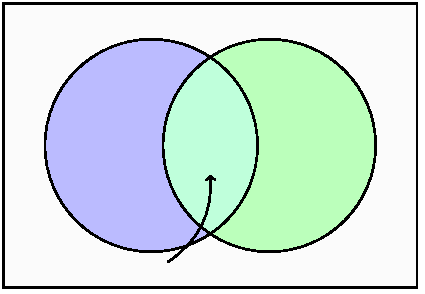
\includegraphics[width=.65\linewidth]{figures/integrality-venn-geometry.pdf}};
  \begin{scope}[x={(venn.south east)},y={(venn.north west)},every node/.style={font=\small,inner sep=0pt,align=center}]
    \node at (.50,.937) {包含 $R$ 的环};
    \node at (.251,.527) {有限生成\\$R$-代数};
    \node at (.755,.500) {$R$ 的整扩张};
    \node at (.386,.071) {有限生成 $R$-模};
  \end{scope}
\end{tikzpicture}\par}

\BookExerciseHeading
\begin{BookExercises}
  \item\label{ex:square-root-of-two-root-test} 元素 $\frac{\sqrt{2}}{2}\in\mathbb{R}$ 在 $\mathbb{Z}$ 上代数吗? 整吗?
  \item\label{ex:rational-integral-iff-integer} 证明 $a\in\mathbb{Q}$ 在 $\mathbb{Z}$ 上整当且仅当 $a\in\mathbb{Z}$. 这说明了\textquotedbl{}整\textquotedbl{}这个术语的由来.
  \item\label{ex:complex-integral-over-real} 证明 $\mathbb{C}$ 在 $\mathbb{R}$ 上整 (或等价地, 代数). (提示: 仿照 Example~\ref{ex:sqrt-two-ring-integral} 的论证.)
  \item\label{ex:classify-integral-polynomial-quotients} 对下列各环, 令 $a=[x]$ 为 $x$ 的陪集, 判定这个环是否在子环 $R[a]$ 上整.
    \begin{enumerate}[label=(\alph*)]
      \item $R[x,y]$
      \item $R[x,y]/\langle y^{2}-x^{2}\rangle$
      \item $R[x,y]/\langle xy\rangle$
      \item $R[x,y,z]/\langle y^{2}-x^{3},z^{3}-x^{4}\rangle$
    \end{enumerate}
  \item\label{ex:rationals-not-finite-module-direct} 由 Example~\ref{ex:rationals-algebraic-not-integral} 可知 $\mathbb{Q}$ 不在 $\mathbb{Z}$ 上整, 所以 Theorem~\ref{thm:finite-generation-integrality} 蕴含 $\mathbb{Q}$ 不是有限生成 $\mathbb{Z}$-模. 请直接验证这一点: 说明对于任意 $a_{1},\ldots,a_{n}\in\mathbb{Q}$, 都有真包含
    \[
      \mathbb{Z}\{a_{1},\ldots,a_{n}\}\subsetneq\mathbb{Q}.
    \]
  \item\label{ex:determinant-cramer-rule} 本题证明 Cramer 法则, 假定读者熟悉矩阵乘法和行列式. 设 $A$ 是元素在环 $R$ 中的 $m\times m$ 矩阵, 向量 $v,w\in R^{m}$ 满足 $Av=w$.
    \begin{enumerate}[label=(\alph*)]
      \item 以 $I_{i}$ 记由 $m\times m$ 单位矩阵 $I$ 将第 $i$ 列替换为 $v$ 而得的矩阵. 证明
        \[
          AI_{i}=A_{i},
        \]
        其中 $A_{i}$ 由 $A$ 将第 $i$ 列替换为 $w$ 而得到.
      \item 用你喜欢的求行列式的方法证明
        \[
          \det(I_{i})=v_{i},
        \]
        再利用行列式的乘法性得出
        \[
          \det(A)\cdot v_{i}=\det(A_{i}).
        \]
    \end{enumerate}
  \item\label{ex:monic-relation-bounds-module-powers} 设 $R\subseteq S$ 为环, $a\in S$. 假设存在 $d$ 次首一多项式 $f\in R[x]$ 使 $f(a)=0$. 证明
    \[
      R[a]=R\{1,a,a^{2},\ldots,a^{d-1}\}.
    \]
    若 $f$ 不首一, 你的证明会在哪一步失效?
  \item\label{ex:integral-closure-is-subring} 设 $R\subseteq S$ 为环. 证明集合 $\{s\in S\mid s\text{ 在 $R$ 上整}\}$ 是 $S$ 中包含 $R$ 的子环. (提示: 使用 Theorem~\ref{thm:finite-generation-integrality}.) 这个子环称为 $R$ 在 $S$ 中的整闭包.
  \item\label{ex:integrality-venn-regions} 令 $R=\mathbb{Z}$. 对本节 \hyperref[fig:integrality-venn-diagram]{Venn 图}中的每个区域, 描述位于该区域中的环 $S$ 的例子.
\end{BookExercises}

\section{Noether 正规化}\label{sec:noether-normalization}

前三节发展了若干模论概念. 现在, 我们将用这些概念研究处于代数几何核心的一类代数对象: 有限生成 $K$-代数.

Noether 正规化定理是关于所有有限生成 $K$-代数的结构定理. 为了说明这一定理所讨论的问题, 回想一下, 有限生成 $K$-代数的典型例子是多项式环
\[
  K[x_{1},\ldots,x_{d}].
\]
并非每个有限生成 $K$-代数都同构于多项式环. Noether 正规化定理试图回答: 用多项式环\textquotedbl{}逼近\textquotedbl{}有限生成 $K$-代数, 究竟能逼近到什么程度? 我们将看到, 给定有限生成 $K$-代数 $A$, 总可以找到子代数 $B\subseteq A$, 使得
\begin{enumerate}
  \item 对某个 $d$, 有 $B\cong K[x_{1},\ldots,x_{d}]$;
  \item $A$ 是有限生成 $B$-模, 或者等价地, $A$ 在 $B$ 上整.
\end{enumerate}
换句话说, Noether 正规化定理保证, 每个有限生成 $K$-代数都是某个多项式环 (最简单的一类 $K$-代数) 上的有限生成模 (最小的一类环扩张).

在陈述并证明 Noether 正规化定理之前, 我们先引入代数独立的概念. 它把线性独立推广到多项式代数的情形, 也便于我们讨论判定子代数何时同构于多项式环的准则.

\begin{Definition}{代数相关与代数独立}\leavevmode\label{def:algebraic-dependence-and-independence}\strut\par\nopagebreak[4]\noindent
设 $A$ 是 $R$-代数. 若存在非零多项式 $f\in R[x_{1},\ldots,x_{d}]$, 使得
\[
  f(a_{1},\ldots,a_{d})=0,
\]
则称元素 $a_{1},\ldots,a_{d}\in A$ 在 $R$ 上\emph{代数相关}. 如果不存在这样的多项式, 则称 $a_{1},\ldots,a_{d}$ 在 $R$ 上\emph{代数独立}.

若集合 $S\subseteq A$ 含有互不相同且在 $R$ 上代数相关的元素 $a_{1},\ldots,a_{d}$, 则称 $S$ 在 $R$ 上\emph{代数相关}. 如果不存在这样的元素, 则称 $S$ 在 $R$ 上\emph{代数独立}.
\end{Definition}

这里的用语有一个细微之处. 元素的列表允许重复, 而集合不计重复. 因此, 即便集合 $\{a_{1},\ldots,a_{d}\}$ 并不代数相关, 元素 $a_{1},\ldots,a_{d}$ 仍可能代数相关. 这种情况恰好发生在这些元素有重复的时候. 例如, 若 $a_{1}=a_{2}=\pi$, 元素 $a_{1}$ 和 $a_{2}$ 在 $\mathbb{Z}$ 上代数相关, 因为非零多项式 $f=x_{1}-x_{2}\in\mathbb{Z}[x_{1},x_{2}]$ 在 $(a_{1},a_{2})$ 处取值为零. 但集合 $\{a_{1},a_{2}\}=\{\pi\}$ 在 $\mathbb{Z}$ 上代数独立. 为避免混淆, 我们会在必要时强调 $a_{1},\ldots,a_{d}$ 互不相同.

由有限个代数独立元素生成的子代数同构于多项式环, 如下一个结论所述. 这是第一同构定理的一个应用 (Exercise~\ref{ex:prove-independent-generators-proposition}).

\begin{Proposition}{代数独立的生成元}\leavevmode\label{prop:algebraically-independent-generators}
设 $A$ 是 $R$-代数. 元素 $a_{1},\ldots,a_{d}\in A$ 在 $R$ 上代数独立, 当且仅当取值映射
\[
  \begin{aligned}
    R[x_{1},\ldots,x_{d}]&\to R[a_{1},\ldots,a_{d}]\subseteq A,\
    f(x_{1},\ldots,x_{d})&\mapsto f(a_{1},\ldots,a_{d})
  \end{aligned}
\]
是 $R$-代数同构.
\end{Proposition}

换句话说, Proposition~\ref{prop:algebraically-independent-generators} 断言, 给定 $R$-代数 $A$, 找到一个同构于多项式环的子代数 $B$, 等价于找到一个由代数独立元素组成的有限集合. 由此引出下面的 Noether 正规化定理, 它对任意域 $K$ 都成立.

\begin{Theorem}{Noether 正规化定理}\leavevmode\label{thm:noether-normalization}
若 $A$ 是有限生成 $K$-代数, 则存在有限子集 $S\subseteq A$, 使得
\begin{enumerate}
  \item[(i)] $S$ 在 $K$ 上代数独立;
  \item[(ii)] $A$ 在 $K[S]$ 上整.
\end{enumerate}
\end{Theorem}

具体地说, 若将定理中集合 $S$ 的各个不同元素写成 $a_{1},\ldots,a_{d}$, 则 $K[a_{1},\ldots,a_{d}]$ 同构于 $d$ 元多项式环, 且 $A$ 在 $K[a_{1},\ldots,a_{d}]$ 上整. 我们未必能找到一个代数独立的有限集合, 使它生成整个 $K$-代数 $A$ (因为 $A$ 未必同构于多项式环). 然而, $A$ 在 $K[a_{1},\ldots,a_{d}]$ 上整, 因而是有限生成 $K[a_{1},\ldots,a_{d}]$-模. 这表明 $a_{1},\ldots,a_{d}$ 所生成的多项式环\textquotedbl{}尽可能接近 $A$\textquotedbl{}.

Noether 正规化定理启发了下面的定义.

\begin{Definition}{Noether 基}\leavevmode\label{def:noether-basis}
设 $A$ 是有限生成 $K$-代数. $A$ 在 $K$ 上的一个\emph{Noether 基}是满足下列条件的有限子集 $S\subseteq A$:
\begin{enumerate}
  \item[(i)] $S$ 在 $K$ 上代数独立;
  \item[(ii)] $A$ 在 $K[S]$ 上整.
\end{enumerate}
\end{Definition}

用 Noether 基的语言来说, Noether 正规化定理就是断言每个有限生成 $K$-代数都存在 Noether 基. 在深入证明这一定理之前, 先来看几个具体的 Noether 基.

\begin{Example}{{\textmd{$K[x,y]/\langle x^{2}+y^{2}-1\rangle$} 的一个 Noether 基}}\leavevmode\label{ex:noether-basis-for-circle}
考虑 $K$-代数
\[
  A=\frac{K[x,y]}{\langle x^{2}+y^{2}-1\rangle}.
\]
注意, $A$ 由 $[x]$ 和 $[y]$ 生成. 但这两个元素并不代数独立, 因为它们满足一个非零的多项式关系:
\[
  [x]^{2}+[y]^{2}-1=[x^{2}+y^{2}-1]=0.
\]
令 $a=[x]\in A$. 我们证明 $\{a\}$ 是 $A$ 的一个 Noether 基.

首先, $a$ 在 $K$ 上代数独立. 为证明这一点, 必须说明对任意非零一元多项式 $f\in K[z]$, 有 $f(a)\neq0$. 注意任意这样的 $f$ 都满足 $f(x)\notin\langle x^{2}+y^{2}-1\rangle$. 因此,
\[
  f(a)=[f(x)]\neq0\in\frac{K[x,y]}{\langle x^{2}+y^{2}-1\rangle}.
\]
其次, 注意到 $K[a]\neq A$, 因为我们无法将 $[y]\in A$ 写成 $a=[x]$ 的多项式表达式. 然而, Example~\ref{ex:circle-coordinate-ring-module} 已经说明, 作为 $K[a]$-模, $A$ 由 $[1]$ 和 $[y]$ 生成:
\[
  A=K[a]\{[1],[y]\}.
\]
这就证明 $A$ 是有限生成 $K[a]$-模, 因此它在 $K[a]$ 上整. 由于 $a$ 在 $K$ 上代数独立, 而 $A$ 在 $K[a]$ 上整, 所以 $\{a\}$ 是一个 Noether 基.

这个例子容易推广到单位 $n$-球面的坐标环
\[
  A=\frac{K[x_{1},\ldots,x_{n}]}{\langle x_{1}^{2}+\cdots+x_{n}^{2}-1\rangle},
\]
从而说明 $\{a_{1}=[x_{1}],\ldots,a_{n-1}=[x_{n-1}]\}$ 是一个 Noether 基 (Exercise~\ref{ex:noether-basis-for-unit-sphere}).
\end{Example}

\begin{Example}{{\textmd{$K[x,y]/\langle xy-1\rangle$} 的一个 Noether 基}}\leavevmode\label{ex:noether-basis-for-hyperbola}
考虑 $K$-代数
\[
  A=\frac{K[x,y]}{\langle xy-1\rangle}.
\]
和 Example~\ref{ex:noether-basis-for-circle} 一样, $A$ 由 $[x]$ 和 $[y]$ 生成, 但这两个元素并不代数独立, 因而不构成 Noether 基. 自然会猜想, 单独取 $[x]$ 或 $[y]$ 也许就能构成 Noether 基. 但事实并非如此. 例如, $[x]$ 固然在 $K$ 上代数独立, 却可以验证 $A$ 不在 $K[x]$ 上整 (Exercise~\ref{ex:hyperbola-not-integral-over-x}).

尽管单独取 $[x]$ 或 $[y]$ 都不能构成 $A$ 的 Noether 基, 但 Noether 正规化定理保证 Noether 基一定存在. 在本例中, 一个 Noether 基由元素 $a=[x+y]$ 给出. 证明的思路见 Exercise~\ref{ex:hyperbola-integral-over-sum}.
\end{Example}

看过几个 Noether 基的例子后, 现在转向 Noether 正规化定理的证明. 证明采用一个巧妙的归纳论证, 其中关键是 Theorem~\ref{thm:finite-generation-integrality}.

\begin{Proof}\textbf{of Theorem~\ref{thm:noether-normalization}.}\quad
按定义, 任意有限生成 $K$-代数都可写成 $A=K[b_{1},\ldots,b_{n}]$, 其中 $b_{1},\ldots,b_{n}\in A$. 我们对生成元的个数 $n$ 归纳.

(归纳起点) 若 $n=0$, 则 $A=K$, 空集就是一个 Noether 基.

(归纳步骤) 假设生成元少于 $n$ 个的所有 $K$-代数都有 Noether 基, 并令 $A=K[b_{1},\ldots,b_{n}]$. 如果 $b_{1},\ldots,b_{n}$ 在 $K$ 上代数独立, 那么 $\{b_{1},\ldots,b_{n}\}$ 就是 $A$ 在 $K$ 上的一个 Noether 基, 结论得证. 于是设 $b_{1},\ldots,b_{n}$ 在 $K$ 上不代数独立, 即存在非零多项式 $f\in K[x_{1},\ldots,x_{n}]$, 使得
\[
  f(b_{1},\ldots,b_{n})=0.
\]
我们将变换这个关系, 得到一个关于 $b_{1}$ 首一的关系.

选取整数 $N$, 使之大于 $f$ 中所有非零系数单项式里出现的最大指数. 定义新元素 $c_{2},\ldots,c_{n}\in A$ 如下:
\[
  c_{2}=b_{2}-b_{1}^{N},\quad c_{3}=b_{3}-b_{1}^{N^{2}},\quad\ldots,\quad
  c_{n}=b_{n}-b_{1}^{N^{n-1}},
\]
因而
\[
  0=f(b_{1},\ldots,b_{n})
  =f\bigl(b_{1},c_{2}+b_{1}^{N},c_{3}+b_{1}^{N^{2}},\ldots,c_{n}+b_{1}^{N^{n-1}}\bigr).
\]
考虑下面的一元多项式
\[
  g(z)=f\bigl(z,c_{2}+z^{N},c_{3}+z^{N^{2}},\ldots,c_{n}+z^{N^{n-1}}\bigr)
  \in K[c_{2},\ldots,c_{n}][z].
\]
注意 $g(b_{1})=0$. 接下来证明 $g$ 的首项系数是单位, 从而 $b_{1}$ 在 $K[c_{2},\ldots,c_{n}]$ 上整.

将 $f$ 的任一单项式 $x_{1}^{\alpha_{1}}\cdots x_{n}^{\alpha_{n}}$ 在 $\bigl(z,c_{2}+z^{N},\ldots,c_{n}+z^{N^{n-1}}\bigr)$ 处取值, 得到
\begin{equation}\label{eq:noether-normalization-evaluated-monomial}
  z^{\alpha_{1}}(c_{2}+z^{N})^{\alpha_{2}}(c_{3}+z^{N^{2}})^{\alpha_{3}}
    \cdots(c_{n}+z^{N^{n-1}})^{\alpha_{n}}.
\end{equation}
合并 $z$ 的同次幂, 可将 \eqref{eq:noether-normalization-evaluated-monomial} 写成
\[
  z^{\alpha_{1}+\alpha_{2}N+\alpha_{3}N^{2}+\cdots+\alpha_{n}N^{n-1}}
  +\text{$z$ 的较低次项}.
\]
由于选取的 $N$ 大于 $\alpha_{1},\ldots,\alpha_{n}$, 指数
\[
  \alpha_{1}+\alpha_{2}N+\alpha_{3}N^{2}+\cdots+\alpha_{n}N^{n-1}
\]
唯一确定 $\alpha_{1},\ldots,\alpha_{n}$. (这个断言就是\textquotedbl{}$N$ 进制展开的唯一性\textquotedbl{}: 例如, 若 $N=10$, 它就是断言一个数的各位数字由这个数本身唯一确定. 参见 Exercise~\ref{ex:uniqueness-of-base-n-expansions}.) 特别地, 对不同的单项式
\[
  x_{1}^{\alpha_{1}}\cdots x_{n}^{\alpha_{n}}\qquad\text{和}\qquad
  x_{1}^{\alpha'_{1}}\cdots x_{n}^{\alpha'_{n}},
\]
在 $\bigl(z,c_{2}+z^{N},\ldots,c_{n}+z^{N^{n-1}}\bigr)$ 处取值后, 得到的 $z$ 的次数不同.

因此, $f$ 中有唯一一个非零系数的单项式使 $\alpha_{1}+\alpha_{2}N+\alpha_{3}N^{2}+\cdots+\alpha_{n}N^{n-1}$ 达到最大. 若 $c\in K$ 是该单项式在 $f$ 中的非零系数, 则 $c$ 也是 $g$ 的首项系数. 所以 $c^{-1}g\in K[c_{2},\ldots,c_{n}][z]$ 是一个在 $b_{1}$ 处取值为零的首一多项式, 因而 $b_{1}$ 在 $K[c_{2},\ldots,c_{n}]$ 上整. 由 Theorem~\ref{thm:finite-generation-integrality} 得到 $K[c_{2},\ldots,c_{n}][b_{1}]$ 在 $K[c_{2},\ldots,c_{n}]$ 上整. 又由于 $b_{1},b_{2},\ldots,b_{n}$ 的多项式组合和 $b_{1},c_{2},\ldots,c_{n}$ 的多项式组合可以相互转换, 有
\[
  K[c_{2},\ldots,c_{n}][b_{1}]=K[b_{1},c_{2},\ldots,c_{n}]
    =K[b_{1},b_{2},\ldots,b_{n}]=A.
\]
于是证明了 $A=K[b_{1},\ldots,b_{n}]$ 在 $K[c_{2},\ldots,c_{n}]$ 上整.

由归纳假设, 存在一个 Noether 基 $S\subseteq K[c_{2},\ldots,c_{n}]$. 我们断言 $S$ 也是 $A$ 的一个 Noether 基. 为此, 需要证明 $S$ 在 $K$ 上代数独立, 且 $A$ 在 $K[S]$ 上整. $S$ 在 $K$ 上代数独立直接来自 $S$ 是 $K[c_{1},\ldots,c_{n}]$ 的一个 Noether 基这一事实. 为证明 $A$ 在 $K[S]$ 上整, 注意下列各环都在它前一个环上整:
\[
  K[S]\subseteq K[c_{2},\ldots,c_{n}]\subseteq A.
\]
其中, 第一个包含关系的整性来自 $S$ 是 $K[c_{1},\ldots,c_{n}]$ 的一个 Noether 基这一假设, 第二个包含关系的整性则是前面论证的核心. 由 Theorem~\ref{thm:finite-generation-integrality}, 这些环中的每一个作为前一个环上的模都是有限生成的. 因此由 Exercise~\ref{ex:finite-module-in-tower} 得到 $A$ 作为 $K[S]$-模有限生成; 再用 Theorem~\ref{thm:finite-generation-integrality}, 得到 $A$ 在 $K[S]$ 上整. 所以 $S$ 是 $A$ 的一个 Noether 基, 归纳论证完成.
\end{Proof}

Noether 正规化定理是过去四节代数理论发展的结晶, 这些努力将带来许多收获. 最直接的一项是, 如下一节所见, Noether 正规化可用来证明零点定理, 从而证明代数与几何的等价性. 收获还不止于此: Noether 正规化也与维数密切相关, 这是下一章要引入的概念. 我们将看到, 若 $X$ 是仿射簇, 则坐标环 $K[X]$ 的任意 Noether 基所含元素的个数等于 $X$ 的维数. 借此可以用 Noether 基证明维数的基本性质.

\BookExerciseHeading
\begin{BookExercises}
  \item\label{ex:prove-independent-generators-proposition} 证明 Proposition~\ref{prop:algebraically-independent-generators}.
  \item\label{ex:noether-basis-for-unit-sphere} 考虑 $K$-代数
  \[
    A=\frac{K[x_{1},\ldots,x_{n}]}{\langle x_{1}^{2}+\cdots+x_{n}^{2}-1\rangle}.
  \]
  对所有 $i=1,\ldots,n-1$, 令 $a_{i}=[x_{i}]$.
  \begin{enumerate}
    \item 证明 $a_{1},\ldots,a_{n-1}$ 代数独立.
    \item 证明 $A$ 在 $K[a_{1},\ldots,a_{n-1}]$ 上整.
  \end{enumerate}
  \item\label{ex:hyperbola-not-integral-over-x} 令 $A=K[x,y]/\langle xy-1\rangle$, 并令 $a=[x]$.
  \begin{enumerate}
    \item 证明 $a$ 在 $K$ 上代数独立.
    \item 证明 $A$ 不在 $K[a]$ 上整.
  \end{enumerate}
  \item\label{ex:hyperbola-integral-over-sum} 令 $A=K[x,y]/\langle xy-1\rangle$, 并令 $a=[x+y]$.
  \begin{enumerate}
    \item 证明 $a$ 在 $K$ 上代数独立.
    \item 证明 $A$ 在 $K[a]$ 上整. (提示: 证明 $[x]$ 和 $[y]$ 都是 $K[a]$ 上首一二次多项式的零点.)
  \end{enumerate}
  \item\label{ex:noether-basis-is-maximal-independent} 设 $A$ 是 $K$-代数. 证明 $A$ 在 $K$ 上的每个 Noether 基都是极大的代数独立集. (换句话说, 真包含一个 Noether 基的任何集合都必定代数相关.)
  \item\label{ex:maximal-independent-need-not-be-noether-basis} 举例说明 Exercise~\ref{ex:noether-basis-is-maximal-independent} 的逆命题不成立. 也就是说, 若 $A$ 是有限生成 $K$-代数, 且 $S$ 是极大的代数独立集, $A$ 不一定在 $K[S]$ 上整.
  \item\label{ex:uniqueness-of-base-n-expansions} 设 $N$ 是正整数, 令 $[N]=\{0,1,\ldots,N-1\}$. 对 $k\geq0$, 考虑函数
  \[
    \begin{aligned}
      \psi_{n}:[N]^{k+1} &\to \mathbb{N},\\
      (\alpha_{0},\ldots,\alpha_{k}) &\mapsto
        \alpha_{0}+\alpha_{1}N+\alpha_{2}N^{2}+\cdots+\alpha_{k}N^{k}.
    \end{aligned}
  \]
  \begin{enumerate}
    \item 若 $N=10$, 你会怎样描述数 $\psi_{k}(\alpha_{0},\ldots,\alpha_{k})$?
    \item 证明对所有 $k\geq0$, $\psi_{k}$ 都是单射. (换句话说, 数 $\alpha_{0}+\alpha_{1}N+\alpha_{2}N^{2}+\cdots+\alpha_{k}N^{k}$ 唯一确定 $\alpha_{0},\ldots,\alpha_{k}$.)
  \end{enumerate}
\end{BookExercises}

\section{零点定理的证明}\label{sec:proof-of-nullstellensatz}

我们现在已经具备了讨论零点定理证明所需的代数工具, 因而可以对第~\ref{chap:varieties-and-ideals}--\ref{chap:polynomial-maps} 章建立的代数与几何的等价性给出完整的论证. 我们先给出两个有用的引理, 借此证明零点定理一个看似较弱的版本. 随后我们将证明, 出人意料的是, 这个弱版本蕴含完整的零点定理.

所需的第一个引理只是告诉我们, 代数闭域没有非平凡的代数域扩张.

\begin{Lemma}{代数闭域上的代数扩张}\leavevmode\label{lem:algebraic-extension-of-algebraically-closed-field}
设 $K\subseteq L$ 为域, 且 $L$ 在 $K$ 上代数. 若 $K$ 是代数闭的, 则 $L=K$.
\end{Lemma}
\begin{Proof}
\BookPairedNote
  {反设 $a\in L\setminus K$. 由于 $a$ 在 $K$ 上代数, 存在多项式 $f\in K[x]$ 使得 $f(a)=0$. 这样的多项式可能有很多, 取其中次数最小的一个作为 $f$. 由于 $K$ 是代数闭的, 存在 $b\in K$ 使 $f(b)=0$.}
  {\textquotedbl{}代数闭\textquotedbl{}这个名称反映了如下事实: 试图向 $K$ 添加一个在 $K$ 上代数的元素时, 所得到的元素其实已在 $K$ 中. 因此 $K$ 对\textquotedbl{}添加代数元\textquotedbl{}是封闭的.}
由 Corollary~\ref{cor:polynomial-factor-theorem}, 可以将 $f(x)$ 分解为
\[
  f(x)=(x-b)g(x),
\]
其中 $g\in K[x]$ 且 $\deg(g)<\deg(f)$. 两边在 $x=a$ 处取值, 得
\[
  0=(a-b)g(a).
\]
我们已假设 $a\notin K$, 且 $b\in K$, 因此 $a\neq b$. 所以上式只有在 $g(a)=0$ 时才成立. 这与 $f$ 是 $K[x]$ 中在 $a$ 处取值为零的次数最小的多项式相矛盾.
\end{Proof}

下一个结论是本节所需的 Noether 正规化定理的主要推论. 它最早由 Zariski 证明, 不过他的方法与这里的方法不同. 这个结论对任意域 $K$ 都成立.

\begin{Lemma}{Zariski 引理}\leavevmode\label{lem:zariski}
设 $K\subseteq L$ 为域. 如果 $L$ 是有限生成 $K$-代数, 则 $L$ 在 $K$ 上代数.
\end{Lemma}
\begin{Proof}
设 $K\subseteq L$ 为域, 且 $L$ 是有限生成 $K$-代数. 对 $L$ 应用 Noether 正规化定理, 可知存在 $d\geq0$ 以及在 $K$ 上代数独立的元素 $a_{1},\ldots,a_{d}\in L$, 使得 $L$ 在 $K[a_{1},\ldots,a_{d}]$ 上整, 因而也代数. 要说明 $L$ 在 $K$ 上代数, 只需证明 $d=0$.

反设 $d>0$. 由于 $L$ 是域, 存在 $a_{1}^{-1}\in L$. 由于 $L$ 在 $K[a_{1},\ldots,a_{d}]$ 上整, 元素 $a_{1}^{-1}$ 是一个系数在 $K[a_{1},\ldots,a_{d}]$ 中的首一多项式的根:
\[
  (a_{1}^{-1})^{m}+c_{1}(a_{1}^{-1})^{m-1}+\cdots
  +c_{m-1}(a_{1}^{-1})+c_{m}=0,
\]
其中 $c_{1},\ldots,c_{m}\in K[a_{1},\ldots,a_{d}]$. 两边同乘 $a_{1}^{m}$, 得
\[
  1+c_{1}a_{1}+\cdots+c_{m-1}a_{1}^{m-1}+c_{m}a_{1}^{m}=0.
\]
这是 $a_{1},\ldots,a_{d}$ 之间的一个多项式关系, 与这些元素的代数独立性矛盾. 因此 $d=0$, 这正是所需结论.
\end{Proof}

下面用前两个引理证明的结论通常称为\textquotedbl{}弱零点定理\textquotedbl{}, 因为如果已经证明了零点定理, 就能相当直接地推出它 (Exercise~\ref{ex:nullstellensatz-implies-weak-nullstellensatz}).

\begin{Proposition}{弱零点定理}\leavevmode\label{prop:weak-nullstellensatz}
设 $K$ 是代数闭的. 对任意真理想 $I\subsetneq K[x_{1},\ldots,x_{n}]$, 都有 $\mathcal{V}(I)\neq\varnothing$.
\end{Proposition}
\begin{Proof}
设 $K$ 是代数闭的, 且 $I\subsetneq K[x_{1},\ldots,x_{n}]$ 是真理想. 由 Exercise~\ref{ex:proper-ideal-contained-in-maximal-ideal}, $K[x_{1},\ldots,x_{n}]$ 存在一个包含 $I$ 的极大理想 $J$. 由于 $I\subseteq J$ 蕴含 $\mathcal{V}(J)\subseteq\mathcal{V}(I)$, 只需证明 $\mathcal{V}(J)\neq\varnothing$.

由于 $J$ 是极大理想, 商环
\[
  L=K[x_{1},\ldots,x_{n}]/J
\]
是域. 此外, $L$ 是有限生成 $K$-代数 (由 $[x_{1}],\ldots,[x_{n}]$ 生成), 因此由 Zariski 引理, $L$ 在 $K$ 上代数. 但 $K$ 是代数闭的, 所以 Lemma~\ref{lem:algebraic-extension-of-algebraically-closed-field} 蕴含 $L=K$.

由于 $L=K$, 存在 $K$-代数同构 $\phi:L\to K$. 定义 $a_{i}=\phi([x_{i}])$. 利用 $\phi$ 是 $K$-代数同态这一事实, 得
\[
  \phi([x_{i}-a_{i}])=\phi([x_{i}])-\phi([a_{i}])=a_{i}-a_{i}=0.
\]
由于 $\phi$ 是单射, 这蕴含对所有 $i$ 都有 $[x_{i}-a_{i}]=0$. 换句话说,
\[
  \langle x_{1}-a_{1},\ldots,x_{n}-a_{n}\rangle\subseteq J.
\]
由于 $\langle x_{1}-a_{1},\ldots,x_{n}-a_{n}\rangle$ 是极大理想, 且 $J$ 是真理想, 可知 $J=\langle x_{1}-a_{1},\ldots,x_{n}-a_{n}\rangle$. 因而
\[
  \mathcal{V}(J)=\{(a_{1},\ldots,a_{n})\}\neq\varnothing,
\]
这就是所需结论.
\end{Proof}

弱零点定理只是一件粗略的工具, 它仅保证 $\mathcal{V}(I)$ 非空. 而 (强) 零点定理却能确切地告诉我们哪些多项式在 $\mathcal{V}(I)$ 上取值为零. 现在我们证明, 这个加强了的结论实际上可由弱零点定理推出. 由于我们在证明弱版本时没有用到强版本, 至此便能完成零点定理的证明.

\begin{Theorem}{回顾零点定理}\leavevmode\label{thm:nullstellensatz-recalled}
设 $K$ 是代数闭域. 则对任意理想 $I\subseteq K[x_{1},\ldots,x_{n}]$, 有
\[
  \mathcal{I}(\mathcal{V}(I))=\sqrt{I}.
\]
\end{Theorem}
\begin{Proof}
包含关系 $\mathcal{I}(\mathcal{V}(I))\supseteq\sqrt{I}$ 在任意域上都成立, 直接由定义得到; 参见 Exercise~\ref{ex:radical-contained-in-vanishing-ideal}. 因此只须证明包含关系 $\mathcal{I}(\mathcal{V}(I))\subseteq\sqrt{I}$. 由于 $K[x_{1},\ldots,x_{n}]$ 是 Noether 环, 可写成 $I=\langle f_{1},\ldots,f_{m}\rangle$.

设 $g\in\mathcal{I}(\mathcal{V}(I))$. 引入新变量 $x_{n+1}$, 考虑理想
\[
  J=\langle f_{1},\ldots,f_{m},h\rangle\subseteq K[x_{1},\ldots,x_{n},x_{n+1}],
\]
其中
\[
  h(x_{1},\ldots,x_{n+1})=1-x_{n+1}g(x_{1},\ldots,x_{n}).
\]
\BookPairedNote
  {我们断言 $\mathcal{V}(J)=\varnothing\subseteq\mathbb{A}^{n+1}$. 为此, 反设 $a=(a_{1},\ldots,a_{n},a_{n+1})\in\mathcal{V}(J)$. 于是对所有 $i$ 都有 $f_{i}(a)=0$. 但 $f_{i}$ 只涉及变量 $x_{1},\ldots,x_{n}$, 所以这等价于对所有 $i$ 都有 $f_{i}(a_{1},\ldots,a_{n})=0$.}
  {添加一个变量的技巧, 是把弱零点定理用于 (强) 零点定理的巧妙手段.}
也就是说, $(a_{1},\ldots,a_{n})\in\mathcal{V}(I)$. 由于 $g\in\mathcal{I}(\mathcal{V}(I))$, 可知 $g(a_{1},\ldots,a_{n})=0$, 因而
\[
  h(a)=1-a_{n+1}g(a_{1},\ldots,a_{n})=1\neq0.
\]
由于 $h\in J$, 这与 $a\in\mathcal{V}(J)$ 矛盾.

我们已经证明 $\mathcal{V}(J)=\varnothing$, 所以弱零点定理蕴含 $J=K[x_{1},\ldots,x_{n+1}]$. 特别地, 常数多项式 $1$ 可用 $J$ 的生成元表示:
\begin{equation}\label{eq:nullstellensatz-unit-ideal-relation}
  1=q_{1}f_{1}+\cdots+q_{m}f_{m}+r(1-x_{n+1}g),
\end{equation}
其中 $q_{1},\ldots,q_{m},r\in K[x_{1},\ldots,x_{n+1}]$. 我们希望在这个等式中把 $g$ 单独分离出来, 但这需要除以 $x_{n+1}$. 为此, 考虑较大的环 $K(x_{n+1})[x_{1},\ldots,x_{n}]$, 其中允许出现关于 $x_{n+1}$ 的有理函数 (我们在 Section~\ref{sec:unique-factorization-polynomial-rings} 中已见过这种环). 等式 \eqref{eq:nullstellensatz-unit-ideal-relation} 在这个较大的环中仍成立. 现在可以把等式两边同除以 $x_{n+1}$ 的一个足够高的幂, 使 $x_{n+1}$ 的正次幂不再出现:
\begin{equation}\label{eq:nullstellensatz-negative-variable-powers}
  x_{n+1}^{-k}=\widetilde{q}_{1}f_{1}+\cdots+\widetilde{q}_{m}f_{m}
    +\widetilde{r}(x_{n+1}^{-1}-g),
\end{equation}
其中 $\widetilde{q}_{1},\ldots,\widetilde{q}_{m},\widetilde{r}\in K[x_{1},\ldots,x_{n},x_{n+1}^{-1}]\subseteq K(x_{n+1})[x_{1},\ldots,x_{n}]$.

现在已经得到多项式环 $K[x_{1},\ldots,x_{n},x_{n+1}^{-1}]$ 中的一个等式. 代入 $x_{n+1}^{-1}=g\in K[x_{1},\ldots,x_{n}]$, 得到
\[
  g^{k}=\widehat{q}_{1}f_{1}+\cdots+\widehat{q}_{m}f_{m},
\]
其中 $\widehat{q}_{i}\in K[x_{1},\ldots,x_{n}]$ 是在 $\widetilde{q}_{i}$ 中令 $x_{n+1}^{-1}=g$ 得到的. 最后这个等式表明 $g^{k}\in I$, 所以 $g\in\sqrt{I}$. 证明完毕.
\end{Proof}

初读时, 证明的最后一步令 $x_{n+1}^{-1}=g$, 常使读者感到可疑: 为什么可以直接给 $x_{n+1}^{-1}$ 选一个值? 我们强调, 这样做成立, 是因为 $x_{n+1}^{-1}$ 在环 $K[x_{1},\ldots,x_{n},x_{n+1}^{-1}]$ 中和其他变量一样, 也是一个变量. 下面在一个小例子中具体展示这一过程.

\begin{Example}{零点定理证明的一个例子}\leavevmode\label{ex:nullstellensatz-proof-illustration}
令 $J=\langle x^{2},y\rangle\subseteq K[x,y]$, 并令 $g=x+y$. 本例中以 $z$ 表示变量 $x_{n+1}$, 等式 \eqref{eq:nullstellensatz-unit-ideal-relation} 就写成
\[
  1=q_{1}(x,y,z)\cdot x^{2}+q_{2}(x,y,z)\cdot y
    +r(x,y,z)\cdot\bigl(1-z(x+y)\bigr),
\]
容易验证, 如下选取 $q_{1},q_{2},r$ 时, 这个等式成立:
\[
  1=(z^{2})\cdot x^{2}+(2xz^{2}+yz^{2})\cdot y
    +(1+xz+yz)\cdot\bigl(1-z(x+y)\bigr).
\]
注意这个等式在 $K[x,y,z]$ 中成立. 在较大的环 $K(z)[x,y]$ 中, 可以把两边同除以 $z^{2}$, 消去 $z$ 的所有正次幂, 得到
\[
  z^{-2}=(1)\cdot x^{2}+(2x+y)\cdot y
    +(z^{-1}+x+y)\cdot\bigl(z^{-1}-(x+y)\bigr),
\]
这个新等式在子环 $K[x,y,z^{-1}]\subseteq K(z)[x,y]$ 中成立. 这个子环就是一个多项式环, 因而可以用其余变量的表达式代替其中一个变量. 代入 $z^{-1}=g=x+y$, 得到
\[
  (x+y)^{2}=(1)\cdot x^{2}+(2x+y)\cdot y,
\]
它显然在 $K[x,y]$ 中成立, 也说明 $g^{2}\in J$.
\end{Example}

\BookExerciseHeading
\begin{BookExercises}
  \item\label{ex:nullstellensatz-implies-weak-nullstellensatz} 证明零点定理蕴含弱零点定理.
  \item\label{ex:weak-nullstellensatz-fails-over-nonclosed-field} 举例说明当 $K$ 不是代数闭的时, 弱零点定理可能不成立. 讨论为什么你的例子虽然不符合弱零点定理, 却仍与 Zariski 引理相容.
  \item\label{ex:proper-ideal-contained-in-maximal-ideal} 设 $I\subseteq K[x_{1},\ldots,x_{n}]$ 为理想, 且 $I\neq K[x_{1},\ldots,x_{n}]$. 证明存在包含 $I$ 的极大理想. (提示: $K[x_{1},\ldots,x_{n}]$ 是 Noether 环, 所以满足升链条件.)
  \item\label{ex:maximal-ideal-geometric-interpretation} 设 $K$ 是代数闭的, 且 $I\subsetneq K[x_{1},\ldots,x_{n}]$ 是真理想.
  \begin{enumerate}
    \item 用仿射簇 $\mathcal{V}(I)$ 和 $\mathcal{V}(J)$ 解释\textquotedbl{}$J$ 是包含 $I$ 的极大理想\textquotedbl{}这一命题.
    \item 利用这一仿射簇解释, 找出两个包含 $I=\langle y^{2}-x^{3}-x^{2}\rangle\subseteq K[x,y]$ 的不同极大理想.
  \end{enumerate}
  \item\label{ex:nullstellensatz-tangent-varieties} 令 $I=\langle x^{2}+y^{2}-1,y-1\rangle\subseteq K[x,y]$, 并令 $g=x\in K[x,y]$.
  \begin{enumerate}
    \item 求 $\mathcal{V}(I)\subseteq\mathbb{A}^{2}$, 并验证 (不引用零点定理) $g\in\mathcal{I}(\mathcal{V}(I))$, 但 $g\notin I$.
    \item 令 $f_{1}=x^{2}+y^{2}-1$ 和 $f_{2}=y-1$ 为 $I$ 的生成元, 并仿照零点定理的证明取 $J=\langle f_{1},f_{2},1-zx\rangle$. 求 $q_{1},q_{2},r\in K[x,y,z]$, 使等式 \eqref{eq:nullstellensatz-unit-ideal-relation} 成立.
    \item 在 (b) 的等式中令 $z=1/g$ 并消去分母, 推出一个表明 $g\in\sqrt{I}$ 的等式.
    \item 你刚刚验证了理想 $I=\langle x^{2}+y^{2}-1,y-1\rangle$ 不是根理想. 另一方面,
    \[
      I=\langle x^{2}+y^{2}-1\rangle+\langle y-1\rangle,
    \]
    因此
    \[
      \mathcal{V}(I)=\mathcal{V}(x^{2}+y^{2}-1)\cap\mathcal{V}(y-1).
    \]
    画出实数域上的 $\mathcal{V}(x^{2}+y^{2}-1)$ 和 $\mathcal{V}(y-1)$. 你能否猜出, 这些簇的什么几何特征导致 $\langle x^{2}+y^{2}-1\rangle+\langle y-1\rangle$ 不是根理想?
  \end{enumerate}
  \item\label{ex:algebraic-closure-from-maximal-ideals} 证明域 $K$ 是代数闭的, 当且仅当每个极大理想 $I\subseteq K[x_{1},\ldots,x_{n}]$ 都具有形式
  \[
    I=\langle x_{1}-a_{1},\ldots,x_{n}-a_{n}\rangle,
  \]
  其中 $a_{1},\ldots,a_{n}\in K$.
\end{BookExercises}


\chapter{维数}\label{chap:dimension}

\noindent\textbf{第 \thechapter{} 章学习目标}
\begin{itemize}
  \item 从直观上描述仿射簇的维数, 并用坐标环中的代数独立性描述它.
  \item 定义仿射簇的函数域, 并在例子中求出函数域.
  \item 用超越基度量域扩张.
  \item 在例子中仔细算出仿射簇的维数.
  \item 用 Noether 正规化定理证明维数论基本定理.
\end{itemize}

给定一组多项式方程, 关于它的解集, 最基本的几何问题大概是这个解集有多\textquotedbl{}大\textquotedbl{}. 本章引入仿射簇维数这个重要概念, 以说明这个问题.

直观上, 维数衡量我们在一个集合中移动的自由度. 那么, 怎样度量在仿射簇中移动的自由度? 我们将看到, 回答这个问题的关键在坐标环里. 本章的一个出发点是: 仿射簇的维数就是其坐标环中代数独立元素的最大个数.

这也许会让读者想起线性代数中的维数: 一个 (有限维) 向量空间的维数可以定义为线性独立元素的最大个数. 本章所发展的许多思想, 确实都与线性代数中关于维数的思想类似. 尤其是第~\ref{sec:transcendence-bases}~节引入的超越基, 其定义和性质与向量空间的基十分相近. 为了建立完善的超越基理论, 我们需要在域而非环中工作. 因此第~\ref{sec:function-fields}~节专门讨论不可约仿射簇的函数域.

在建立函数域和超越基的基础之后, 第~\ref{sec:dimension-of-affine-varieties}~节将定义维数, 并描述它的一些基本性质. 例如, 我们会看到 $\dim(\mathbb{A}^{n})=n$; 若 $X\subseteq Y$, 则 $\dim(X)\leq\dim(Y)$. 本章的思想最终汇聚于第~\ref{sec:fundamental-theorem-of-dimension-theory}~节, 得到我们所称的维数论基本定理. 这个代数几何中的核心结果大意是: 一组多项式方程中, 每增加一个方程, 解集的维数至多降低一.

\par\smallskip
{\footnotesize
\noindent\textcopyright{} The Author(s) 2025\par
\noindent E. Clader, D. Ross, \emph{Beginning in Algebraic Geometry}, Undergraduate Texts in Mathematics,
\href{https://doi.org/10.1007/978-3-031-88819-9_7}{\nolinkurl{https://doi.org/10.1007/978-3-031-88819-9_7}}.\par}

\section{引入维数的想法}\label{sec:motivation-for-dimension}

维数是一个人人都很熟悉的概念. 例如, 我们大多数人大概从小就明白, 自己生活在一个三维世界里. 我们对这三个维度的理解是, 我们有三个基本的移动方向: 前后, 左右和上下. 当然, 方向并不只有这三种, 但任何其他方向都是这三种方向的组合.

\BookPairedFigure
  {对我们许多人来说, 线性代数是第一次学到维数的精确定义的数学学科. 这一定义自然体现了上一段提到的\textquotedbl{}基本\textquotedbl{}和\textquotedbl{}组合\textquotedbl{}两个概念. 回忆一下, 若域 $K$ 上的向量空间 $V$ 有一组含 $n$ 个向量的基, 就称其维数为 $n$. 重要的是, 必须检查 $V$ 的任何两组基都有相同数目的向量, 这样才能保证这一定义是良定义的. 可以把基向量看成在 $V$ 中移动的基本方向.}
  {\phantomsection\label{fig:dimension-standard-basis}%
   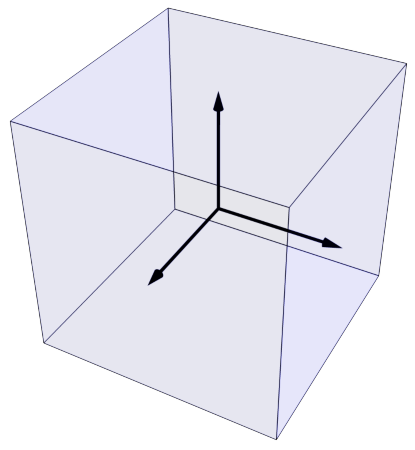
\includegraphics[width=\linewidth]{figures/dimension-standard-basis.png}}
\noindent\hyperref[fig:dimension-standard-basis]{上图}画出了 $\mathbb{R}^{3}$ 的三个标准基向量. 在 $\mathbb{R}^{3}$ 中移动的任意方向, 都可以唯一表示成这三个向量的线性组合.

\BookPairedNoteLeft
  {维数衡量在一个集合中移动的自由度, 这个直观想法将指导我们给出代数几何中的维数定义. 下面用一个熟悉的非线性例子进一步说明.}
  {注意域 $K$ 对向量空间维数的重要作用: 通常的平面作为 $\mathbb{R}$-向量空间是二维的, 但作为 $\mathbb{C}$-向量空间只有一维.}

\begin{Example}{球面的维数}\leavevmode\label{ex:dimension-of-the-sphere}
考虑球面 $X=\mathcal{V}(x^{2}+y^{2}+z^{2}-1)\subseteq\mathbb{A}^{3}$. 在实数域上, 这就是熟悉的单位球面. 甚至可以把单位球面想象成地球表面的模型.

\BookPairedFigure
  {我们自然会认为地球表面是二维的, 因为在任何位置, 我们都有两个基本的移动方向. 当不在两极时, 我们称这两个方向为南北方向和东西方向. 但是, 如何用代数精确刻画日常经验中这两个维度的自由度?}
  {\phantomsection\label{fig:dimension-blue-marble}%
   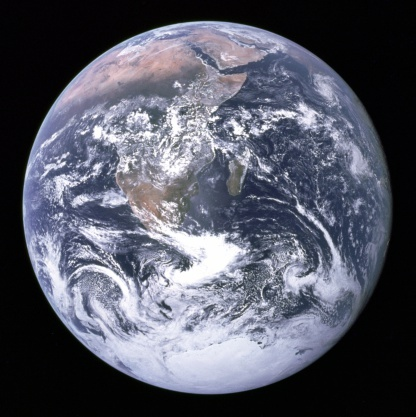
\includegraphics[width=\linewidth]{figures/dimension-blue-marble.jpg}\par
   {\footnotesize\emph{The Blue Marble}\\NASA 摄\par}}

可以这样论证: 若选定 $X$ 中一点的两个坐标, 比如令 $x=a$ 且 $y=b$, 其中 $a,b\in K$, 那么由 $X$ 的定义方程可知, 第三个坐标受这两个选择的约束, 必须满足
\[
  z^{2}=1-a^{2}-b^{2}.
\]
特别地, 第三个坐标至多有两个可能的解.

换句话说, 要描述 $X$ 上的一个点, 有两个可以自由取值的变量: 可以不受约束地选择 $x$ 和 $y$ 坐标, 而第三个坐标随之只能取有限个可能的值. 这反映出一个代数事实: 元素 $[x],[y]\in K[X]$ 在 $K$ 上代数独立, 因为指定其中一个的值不会约束另一个. 而 $[x],[y],[z]$ 在 $K$ 上代数相关, 因为它们满足多项式关系
\[
  [x]^{2}+[y]^{2}+[z]^{2}-1=[x^{2}+y^{2}+z^{2}-1]=0\in K[X].
\]
\end{Example}

上一个例子表明, 在 $X$ 中\textquotedbl{}移动的自由度\textquotedbl{}可以用代数独立的函数来度量: 只要 $K[X]$ 中有代数独立的坐标函数, 就可以不受约束地选择这些坐标的值. 由于维数应当度量我们所能具有的最大移动自由度, 便得到以下想法.

\begin{BookKeyIdea}{仿射簇的维数}\leavevmode\label{idea:dimension-as-algebraic-independence}
仿射簇 $X$ 的维数应当等于 $K[X]$ 中在 $K$ 上代数独立的元素的最大个数.
\end{BookKeyIdea}

其实, 可以用这个想法定义维数. 我们不这样做, 是因为这个定义不太便于使用. 首先, 按这种描述甚至不清楚维数是否有限: 给定仿射簇 $X$, 如何知道 $K[X]$ 中不可能找到越来越大的代数独立函数集? 要证明这种情形不可能发生, 得先做一些准备. 第~\ref{sec:function-fields}--\ref{sec:transcendence-degree}~节将仔细完成这些准备. 然后第~\ref{sec:dimension-of-affine-varieties}~节会给出一个更便于使用的维数定义, 并证明它与上面的描述等价 (Corollary~\ref{cor:dimension-and-algebraic-independence}).

先把 Key Idea~\ref{idea:dimension-as-algebraic-independence} 作为动机记在心里, 转而讨论我们希望维数具备什么性质. 仿射簇的维数应当满足哪些基本性质? 我们先列出这些性质, 称之为维数公理.

\begin{Definition}{仿射簇的维数公理}\leavevmode\label{def:axioms-for-dimension}
如果函数
\[
  D:\left\{\text{非空仿射簇的同构类}\right\}\longrightarrow\mathbb{N}
\]
满足下列性质, 则称它为\emph{维数函数}:
\begin{enumerate}
  \item\label{ax:dimension-of-a-point} 若 $X$ 只含一个点, 则 $D(X)=0$;
  \item\label{ax:dimension-of-a-finite-union} $D(X_{1}\cup\cdots\cup X_{n})=\max\{D(X_{1}),\ldots,D(X_{n})\}$;
  \item\label{ax:dimension-of-a-hypersurface-section} 若 $X\subseteq\mathbb{A}^{n}$ 不可约, 且 $f\in K[x_{1},\ldots,x_{n}]$ 使得 $X\cap\mathcal{V}(f)$ 非空且不等于整个 $X$, 则 $D(X\cap\mathcal{V}(f))=D(X)-1$.
\end{enumerate}
\end{Definition}

简要解释一下这些维数公理. 首先, 两个同构的仿射簇具有相同的本质性质, 所以可以预期它们的维数相同. 这就是为什么我们把维数看成定义在仿射簇同构类集合上的函数. 由直观也不难看出为何要求公理~\ref{ax:dimension-of-a-point}: 在单个点上没有移动的自由, 所以一个点的维数应为零.

关于公理~\ref{ax:dimension-of-a-finite-union}, 以 $\mathbb{A}^{3}$ 中一条直线 $L$ 和一个平面 $P$ 的并为例. 如果直线包含在平面内, 它们的并就是这个平面, 因此 $\dim(L\cup P)=\dim(P)$, 即两个维数中的较大者. 然而, 如果直线不包含在平面内, \textquotedbl{}移动的自由度\textquotedbl{}这一直观想法就失效了: 在 $L\cup P$ 中能往多少个方向移动, 取决于站在哪一点. 为消除这种歧义, 我们规定取两者中较大的维数. 更一般地说, 我们会发现只有在不可约簇上才容易定义维数, 而可约簇的维数将定义为其不可约分支的维数的最大值.

最后来看公理~\ref{ax:dimension-of-a-hypersurface-section}. 将 $X$ 写成零点集 $\mathcal{V}(f_{1},\ldots,f_{m})$, 就能进一步分析这一陈述. 此时
\[
  X\cap\mathcal{V}(f)=\mathcal{V}(f_{1},\ldots,f_{m},f).
\]
换句话说, 公理~\ref{ax:dimension-of-a-hypersurface-section} 的实质是: 若再加上一个方程, 维数恰好降低一. 这个维数性质在代数几何中的重要性怎么强调都不为过. 因此, 本书称这一性质为\emph{维数论基本定理}.

\begin{BookFlowNote}[l]{%
公理~\ref{ax:dimension-of-a-hypersurface-section} 的所有假设都是必要的. 假设 $X$ 不可约, 是因为否则 $X$ 可能由两个相同维数的不可约分支组成, 而与 $\mathcal{V}(f)$ 相交时可能只选出其中一个分支.
}
\noindent 在向量空间的情形, 公理~\ref{ax:dimension-of-a-hypersurface-section} 是秩--零度定理的推论 (见 Exercise~\ref{ex:dimension-axiom-vector-space-analogue}).

例如, 在 $\mathbb{A}^{2}$ 中, 一维簇 $X=\mathcal{V}(xy)$ 是两个坐标轴的并. 与 $\mathcal{V}(x)$ 相交, 只选出一维的 $y$ 轴, 有违公理~\ref{ax:dimension-of-a-hypersurface-section} 的结论. 我们假设 $X\cap\mathcal{V}(f)$ 非空, 是因为 $\varnothing$ 没有定义维数. 我们还假设 $X\cap\mathcal{V}(f)\neq X$, 因为如果两者相等, 公理~\ref{ax:dimension-of-a-hypersurface-section} 的结论就不成立.
\end{BookFlowNote}

人们自然会问, 为什么不为维数再加几条公理. 例如, 我们或许会自然地假定 $\mathbb{A}^{n}$ 的维数为 $n$; 更一般地, 由线性方程定义的仿射簇的维数应当等于它作为向量空间的维数. 我们不作更多假设, 是因为 Definition~\ref{def:axioms-for-dimension} 中为数不多的几条公理已经唯一决定了所有仿射簇的维数, 如下所述.

\begin{Proposition}{维数函数至多有一个}\leavevmode\label{prop:uniqueness-of-dimension}
若 $D_{1}$ 和 $D_{2}$ 都是维数函数, 则对所有仿射簇 $X$ 都有 $D_{1}(X)=D_{2}(X)$.
\end{Proposition}
\begin{Proof}
证明的思路见 Exercise~\ref{ex:prove-dimension-function-unique}.
\end{Proof}

根据 Proposition~\ref{prop:uniqueness-of-dimension}, 接下来的路线已经清楚了: 我们要定义一个函数
\[
  D:\left\{\text{非空仿射簇的同构类}\right\}\longrightarrow\mathbb{N},
\]
并证明它满足 Definition~\ref{def:axioms-for-dimension} 的公理~\ref{ax:dimension-of-a-point}--\ref{ax:dimension-of-a-hypersurface-section}. 接下来三节将发展定义维数所需的代数工具. 重点是进一步理解代数相关与代数独立, 并发展超越次数这个关键概念. 第~\ref{sec:dimension-of-affine-varieties}~节用超越次数严格定义维数后, 公理~\ref{ax:dimension-of-a-point} 和~\ref{ax:dimension-of-a-finite-union} 的证明将很直接. 实际上, 用 Key Idea~\ref{idea:dimension-as-algebraic-independence} 就已经能证明它们 (见 Exercise~\ref{ex:point-has-dimension-zero-by-independence}, \ref{ex:dimension-monotonic-by-independence} 和~\ref{ex:dimension-of-union-by-independence}). 相比之下, 证明公理~\ref{ax:dimension-of-a-hypersurface-section} 要复杂得多, 其中一个关键步骤用到 Noether 正规化定理. 我们将在第~\ref{sec:fundamental-theorem-of-dimension-theory}~节完成这项工作.

\BookExerciseHeading
\begin{BookExercises}
  \item\label{ex:point-has-dimension-zero-by-independence} 假设 Key Idea~\ref{idea:dimension-as-algebraic-independence}, 证明一个点的维数为零.
  \item\label{ex:affine-space-dimension-lower-bound} 假设 Key Idea~\ref{idea:dimension-as-algebraic-independence}, 证明 $\dim(\mathbb{A}^{n})\geq n$.
  \item\label{ex:dimension-monotonic-by-independence} 设 $X,Y\subseteq\mathbb{A}^{n}$ 是仿射簇, 且 $X\subseteq Y$.
  \begin{enumerate}
    \item 设 $f_{1},\ldots,f_{m}\in K[x_{1},\ldots,x_{n}]$ 是多项式, 且
    \[
      f_{1}|_{X},\ldots,f_{m}|_{X}\in K[X]
    \]
    在 $K$ 上代数独立. 证明
    \[
      f_{1}|_{Y},\ldots,f_{m}|_{Y}\in K[Y]
    \]
    在 $K$ 上代数独立.
    \item 假设用 Key Idea~\ref{idea:dimension-as-algebraic-independence} 得到 $\dim(X)=d_{1}$ 且 $\dim(Y)=d_{2}$. 证明 $d_{1}\leq d_{2}$.
  \end{enumerate}
  \item\label{ex:dimension-of-union-by-independence} 设 $X_{1},\ldots,X_{m}\subseteq\mathbb{A}^{n}$ 是仿射簇, 令 $X=X_{1}\cup\cdots\cup X_{m}$.
  \begin{enumerate}
    \item 设 $f_{1},\ldots,f_{\ell}\in K[x_{1},\ldots,x_{n}]$ 是多项式, 且
    \[
      f_{1}|_{X},\ldots,f_{\ell}|_{X}\in K[X]
    \]
    在 $K$ 上代数独立. 证明对某个 $i$,
    \[
      f_{1}|_{X_{i}},\ldots,f_{\ell}|_{X_{i}}\in K[X_{i}]
    \]
    在 $K$ 上代数独立.
    \item 假设用 Key Idea~\ref{idea:dimension-as-algebraic-independence} 得到 $\dim(X_{i})=d_{i}$, $i=1,\ldots,m$. 证明
    \[
      \dim(X)=\max\{d_{1},\ldots,d_{m}\}.
    \]
    (提示: 一个不等式用 (a), 另一个用上一题.)
  \end{enumerate}
  \item\label{ex:dimension-function-of-affine-space} 设 $D$ 是维数函数. 证明 $D(\mathbb{A}^{n})=n$.
  \item\label{ex:dimension-axiom-vector-space-analogue} 设 $\ell_{1},\ldots,\ell_{m}$ 是 $n$ 元齐次线性多项式, 考虑由它们的共同零点定义的线性子空间 $V\subseteq K^{n}$:
  \[
    V=\mathcal{V}(\ell_{1},\ldots,\ell_{m})\subseteq\mathbb{A}^{n}=K^{n}.
  \]
  \begin{enumerate}
    \item 将 $V$ 解释成某个具体矩阵 $M$ 的核, 并用秩--零度定理将 $V$ 的维数表示成 $n$ 和 $\operatorname{rk}(M)$ 的函数.
    \item 设 $\ell$ 是另一个齐次线性方程, 考虑子空间
    \[
      W=V\cap\mathcal{V}(\ell).
    \]
    将 $W$ 解释成某个具体矩阵 $M'$ 的核. $M$ 和 $M'$ 有何关系?
    \item 利用 $M$ 和 $M'$ 的关系, 说明 $V$ 和 $W$ 的维数有何关系. 这与 Definition~\ref{def:axioms-for-dimension} 中的公理~\ref{ax:dimension-of-a-hypersurface-section} 相比如何?
  \end{enumerate}
  (提示: (c) 要考虑两种可能的情形. 是哪两种?)
  \item\label{ex:proper-nonempty-hypersurface-section} 设 $X\subseteq\mathbb{A}^{n}$ 是不只含一个点的不可约仿射簇. 证明存在 $f\in K[x_{1},\ldots,x_{n}]$ 使得
  \[
    \varnothing\subsetneq X\cap\mathcal{V}(f)\subsetneq X.
  \]
  (本题有助于做下一题.)
  \item\label{ex:prove-dimension-function-unique} 设 $D_{1}$ 和 $D_{2}$ 是维数函数.
  \begin{enumerate}
    \item 证明 $D_{1}(X)=0$ 当且仅当 $X$ 是有限个点的并, 由此得出: 只要 $D_{1}(X)=0$, 就有 $D_{1}(X)=D_{2}(X)$.
    \item 设 $m\geq1$, 并假设 $D_{1}(X)<m$ 时 $D_{1}(X)=D_{2}(X)$. 证明对所有满足 $D_{1}(X)=m$ 的 $X$, 都有 $D_{1}(X)=D_{2}(X)$.
    \item 将 (a) 和 (b) 合起来, 给出 Proposition~\ref{prop:uniqueness-of-dimension} 的归纳证明.
  \end{enumerate}
  \item\label{ex:dimension-function-need-not-exist-over-reals} 本题证明当 $K$ 不是代数闭的时, 维数函数不一定存在. 令 $K=\mathbb{R}$, 并反设存在维数函数 $D$.
  \begin{enumerate}
    \item 证明 $D(\mathbb{A}^{2})=2$ 且 $D(\{(0,0)\})=0$.
    \item 证明存在 $f$ 使得 $\{(0,0)\}=\mathcal{V}(f)\cap\mathbb{A}^{2}$.
    \item 说明 (a) 和 (b) 与 Definition~\ref{def:axioms-for-dimension} 的公理~\ref{ax:dimension-of-a-hypersurface-section} 矛盾.
  \end{enumerate}
\end{BookExercises}

\par\medskip
{\footnotesize
\noindent\textbf{开放获取.} 本章按照
\href{http://creativecommons.org/licenses/by-nc/4.0/}{Creative Commons Attribution-NonCommercial 4.0 International License}
的条款授权. 该许可允许以任何媒介或格式进行非商业性使用, 分享, 改编, 分发和复制, 但须对原作者和来源作适当署名, 提供 Creative Commons 许可的链接, 并说明是否作了修改.

\noindent
\begin{minipage}[t]{.17\linewidth}
  \vspace{0pt}
\includegraphics[width=.9\linewidth]{figures/source-cc-by-nc.png}
\end{minipage}\hfill
\begin{minipage}[t]{.81\linewidth}
  \vspace{0pt}本章的图片或其他第三方材料均纳入本章的 Creative Commons 许可, 除非材料的署名行另有注明. 如果材料未纳入本章的 Creative Commons 许可, 且您拟进行的使用未获法律规定的许可或超出允许使用的范围, 则须直接向著作权持有人取得许可.
\end{minipage}\par}

\section{函数域}\label{sec:function-fields}

上一节说过, 仿射簇的维数应当衡量其坐标环中代数独立元素的最大个数. 然而, 在 $K$-代数中处理代数相关与代数独立往往相当困难, 而在 $K$ 的域扩张中处理这些概念则容易许多. 因此, 本节研究怎样从不可约仿射簇 $X$ 过渡到一个相应的域 $K(X)$, 即它的函数域.

\begin{Definition}{函数域}\leavevmode\label{def:function-field}
设 $X$ 是不可约仿射簇. $X$ 的\emph{函数域}记为 $K(X)$, 它是 $X$ 的坐标环的分式域:
\[
  K(X)=\operatorname{Frac}(K[X]).
\]
$K(X)$ 的元素称为 $X$ 上的\emph{有理函数}.
\end{Definition}

回忆一下, 分式域在第~\ref{sec:unique-factorization-polynomial-rings}~节定义. 我们在那里知道, $K(X)$ 的元素是 $f/g$ 形式的商, 其中 $f,g\in K[X]$ 且 $g\neq0$. 两个分式 $f_{1}/g_{1}$ 和 $f_{2}/g_{2}$ 相等, 当且仅当 $f_{1}g_{2}=f_{2}g_{1}\in K[X]$. 分式域的确是一个域, 其加法与乘法定义为
\[
  \frac{f_{1}}{g_{1}}+\frac{f_{2}}{g_{2}}
    =\frac{f_{1}g_{2}+f_{2}g_{1}}{g_{1}g_{2}}
  \qquad\text{和}\qquad
  \frac{f_{1}}{g_{1}}\cdot\frac{f_{2}}{g_{2}}=\frac{f_{1}f_{2}}{g_{1}g_{2}}.
\]
由于只有整环才有分式域 (Exercise~\ref{ex:fraction-field-needs-domain}), 函数域只对不可约仿射簇定义. 来看几个例子.

\begin{Example}{仿射空间的函数域}\leavevmode\label{ex:function-field-of-affine-space}
由于 $\mathbb{A}^{n}$ 的坐标环是 $K[x_{1},\ldots,x_{n}]$, 它的函数域就是通常的有理函数域
\[
  K(\mathbb{A}^{n})=K(x_{1},\ldots,x_{n}),
\]
我们已经在第~\ref{sec:unique-factorization-polynomial-rings}~节遇到过它.
\end{Example}

\begin{Example}{$\mathcal{V}(x^{2}-y^{3})$ 的函数域}\leavevmode\label{ex:function-field-of-cusp}
令 $X=\mathcal{V}(x^{2}-y^{3})\subseteq\mathbb{A}^{2}$. 计算坐标环, 得到
\[
  K[X]=K[x,y]/\langle x^{2}-y^{3}\rangle
  \quad\Longrightarrow\quad
  K(X)=\operatorname{Frac}(K[x,y]/\langle x^{2}-y^{3}\rangle).
\]
这看上去是个相当复杂的域, 但我们可以把它与一个更熟悉的域认同. 考虑 $K$-代数同态
\[
  \begin{aligned}
    \phi:K[X]&\to K[t],\\
    [f(x,y)]&\mapsto f(t^{3},t^{2}).
  \end{aligned}
\]
这是 Example~\ref{ex:cusp-bijective-map-not-isomorphism} 所定义的多项式映射的拉回. 注意 $\phi$ 是单射, 但不是同构, 因为多项式 $t$ 不在它的像里.

过渡到函数域, 就能把 $\phi$ 扩张成域同态
\[
  \begin{aligned}
    \overline{\phi}:K(X)&\to K(t),\\
    \frac{[f(x,y)]}{[g(x,y)]}&\mapsto\frac{f(t^{3},t^{2})}{g(t^{3},t^{2})}.
  \end{aligned}
\]
现在可以做除法了, 就会发现 $t$ 实际上在 $\overline{\phi}$ 的像中:
\[
  t=\frac{\phi([x])}{\phi([y])}
    =\overline{\phi}\left(\frac{[x]}{[y]}\right).
\]
这样便能求出 $\overline{\phi}$ 的逆:
\[
  \overline{\phi}^{-1}\left(\frac{f(t)}{g(t)}\right)
    =\frac{f([x]/[y])}{g([x]/[y])}
    =\frac{[y^{\max(\deg(f),\deg(g))}f(x/y)]}
          {[y^{\max(\deg(f),\deg(g))}g(x/y)]},
\]
其中第二个等号只是清除 $f$ 和 $g$ 中的分母, 使像显式地表示成 $K(X)$ 的一个元素. 由此得到 $K(X)\cong K(t)$. 建议读者在 Exercise~\ref{ex:verify-cusp-function-field-isomorphism} 中检查论证的细节.

这个例子表明, 尽管 $X$ 与 $\mathbb{A}^{1}$ 不同构, 它们的函数域却同构, 因为两者都同构于 $K(t)$. 因此, 尽管坐标环包含了关于仿射簇同构类的全部信息, 过渡到函数域时却会丢掉一部分信息.
\end{Example}

\begin{BookFlowNote}[l]{%
在前两个例子中, 所考察的两个函数域都同构于通常的有理函数域 $K(x_{1},\ldots,x_{d})$, 其中 $d$ 为某个整数. 若一个不可约簇的函数域同构于通常的有理函数域, 就称这个簇为\emph{有理}的.
}
\noindent 尽管具有同构函数域的仿射簇未必同构, 第~\ref{chap:rational-maps}~章将说明它们\textquotedbl{}双有理\textquotedbl{}.

事实上有理簇相当特殊. 本书范围之外的一个一般事实是, \textquotedbl{}大多数\textquotedbl{}簇都不是有理的. 特别是, 若 $f\in K[x_{1},\ldots,x_{n}]$ 是一个次数足够高的\textquotedbl{}随机\textquotedbl{}多项式, 则 $\mathcal{V}(f)$ 不是有理的. 下一个例子或许是最简单的非有理簇例子.
\end{BookFlowNote}

\begin{Example}{$\mathcal{V}(x^{3}+y^{3}+1)$ 不是有理的}\leavevmode\label{ex:fermat-cubic-not-rational}
\BookPairedFigure
  {置 $K=\mathbb{C}$, 令 $X=\mathcal{V}(x^{3}+y^{3}+1)\subseteq\mathbb{A}^{2}$. $X$ 的实点在\hyperref[fig:nonrational-cubic-real-points]{右图}中画出. 我们证明 $X$ 不是有理的. 论证的关键在于以下事实: 若非零多项式 $f_{1},f_{2},f_{3}\in K[x_{1},\ldots,x_{n}]$ 满足 (i) 任意两个都没有公共不可约因子, 且 (ii) $f_{1}^{3}+f_{2}^{3}+f_{3}^{3}=0$, 则 $f_{1},f_{2},f_{3}$ 必须都是常数 (证明见 Exercise~\ref{ex:polynomial-fermat-cubes}).}
  {\phantomsection\label{fig:nonrational-cubic-real-points}%
   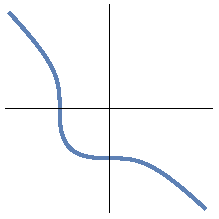
\includegraphics[width=\linewidth]{figures/function-field-nonrational-curve.pdf}}
要证明 $X$ 不是有理的, 首先注意到 $x^{3}+y^{3}+1$ 不可约, 因此
\[
  \begin{gathered}
    K[X]=K[x,y]/\langle x^{3}+y^{3}+1\rangle\\
    \Longrightarrow\quad K(X)=\operatorname{Frac}(K[x,y]/\langle x^{3}+y^{3}+1\rangle).
  \end{gathered}
\]
设
\[
  \phi:K(X)\to K(x_{1},\ldots,x_{d})
\]
对某个 $d>0$ 是域同态. 我们证明 $\operatorname{im}(\phi)\subseteq K$, 从而 $\phi$ 不可能是同构. 注意 $\phi([x])=f/g$ 且 $\phi([y])=h/k$, 其中 $f,g,h,k\in K[x_{1},\ldots,x_{d}]$ 是多项式, $g,k\neq0$. 由于 $K[x_{1},\ldots,x_{n}]$ 是 UFD, 我们可以将每个多项式分解成不可约因子的乘积并约分. 换句话说, 可以假设 $f$ 和 $g$ 之间, 以及 $h$ 和 $k$ 之间, 都没有公共不可约因子. 由 $[x^{3}+y^{3}+1]=0\in K(X)$ 得到关系
\[
  0=\phi([x^{3}+y^{3}+1])
    =\left(\frac{f}{g}\right)^{3}+\left(\frac{h}{k}\right)^{3}+1.
\]
消去分母得
\begin{equation}\label{eq:nonrational-cubic-cleared-denominators}
  (fk)^{3}+(gh)^{3}+(gk)^{3}=0.
\end{equation}
等式 \eqref{eq:nonrational-cubic-cleared-denominators} 给出 $g^{3}\mid(fk)^{3}$. 由于假设 $f$ 和 $g$ 没有公共不可约因子, 所以 $g^{3}\mid k^{3}$. 类似地, 可得 $k^{3}\mid g^{3}$. 因此, 由 $g^{3}\mid k^{3}$ 和 $k^{3}\mid g^{3}$ 知道 $g^{3}=ak^{3}$, 其中 $a$ 为常数. 将其代入等式 \eqref{eq:nonrational-cubic-cleared-denominators} 并约去 $k^{3}$, 得到关系
\begin{equation}\label{eq:nonrational-cubic-coprime-relation}
  f^{3}+ah^{3}+g^{3}=0.
\end{equation}
注意 $g$ 的不可约因子和 $k$ 的不可约因子相同, 因而按假设, 它们既不是 $f$ 的不可约因子, 也不是 $h$ 的不可约因子. 此外, $f$ 和 $h$ 不能有公共不可约因子, 否则由等式 \eqref{eq:nonrational-cubic-coprime-relation}, 它也会是 $g$ 的不可约因子, 与关于 $f$ 和 $g$ 的假设矛盾. 因此, 等式 \eqref{eq:nonrational-cubic-coprime-relation} 中任意两项都没有公共不可约因子, 可以应用 Exercise~\ref{ex:polynomial-fermat-cubes} 得到 $f,g,h,k$ 都是常数, 正如所断言的那样.

上面的论证表明, 对任意 $d>0$, $K(X)$ 都与 $K(x_{1},\ldots,x_{d})$ 不同构. 但若 $d=0$ 呢? 由于 $X$ 有不止一个点, 可知 $K\subsetneq K[X]$, 这蕴含 $K\subsetneq K(X)$, 从而 $K(X)$ 与 $K$ 不同构. 结合前面的论证, 可知 $X$ 不是有理的.
\end{Example}

最后对术语作一个简短说明: 虽然 $K(X)$ 的元素称为有理函数, 但它们实际上不是 $X$ 上的函数. 具体地说, 给定 $f/g\in K(X)$ 且 $g\neq0$, 对某些 (但非全部) $a\in X$, 可能有 $g(a)=0$. 因而 $f/g$ 只在 $X$ 中满足 $g\neq0$ 的子集上定义了一个函数. 通常用虚线箭头表示有理函数, 提醒读者它们并非在整个定义域上都有定义:
\[
  \frac{f}{g}:X\mathrel{\rightdasharrow}K.
\]
若把定义域限制为 $\mathcal{V}(g)$ 的补集, 则每个有理函数都会给出一个真正的函数, 为定义域的每个元素指定一个值:
\[
  \frac{f}{g}:X\setminus\mathcal{V}(g)\longrightarrow K.
\]
这个概念和记号将在第~\ref{sec:rational-maps-between-varieties}~节大幅推广.

\BookExerciseHeading
\begin{BookExercises}
  \item\label{ex:hyperbola-function-field} 令 $X=\mathcal{V}(xy-1)\subseteq\mathbb{A}^{2}$. 证明 $K(X)\cong K(t)$.
  \item\label{ex:extend-injection-to-fraction-fields} 设 $R$ 和 $S$ 为整环, 且 $\phi:R\to S$ 为单射环同态. 证明存在良定义的域同态
  \[
    \begin{aligned}
      \overline{\phi}:\operatorname{Frac}(R)&\to\operatorname{Frac}(S),\\
      \frac{a}{b}&\mapsto\frac{\phi(a)}{\phi(b)}.
    \end{aligned}
  \]
  \item\label{ex:verify-cusp-function-field-isomorphism} 设 $\phi$ 和 $\overline{\phi}$ 为 Example~\ref{ex:function-field-of-cusp} 中的同态.
  \begin{enumerate}
    \item 证明 $\phi$ 是单射, 并用这一点证明 $\overline{\phi}$ 是良定义的.
    \item 证明 $\overline{\phi}$ 和 $\overline{\phi}^{-1}$ 的确是互逆的域同态.
  \end{enumerate}
  \item\label{ex:polynomial-fermat-cubes} 假设 $\operatorname{char}(K)\neq3$. 设 $f_{1},f_{2},f_{3}\in K[x_{1},\ldots,x_{n}]$ 是非零多项式, 满足 (i) 任意两个都没有公共不可约因子, 且 (ii) $f_{1}^{3}+f_{2}^{3}+f_{3}^{3}=0$. 本题勾勒 $f_{1},f_{2},f_{3}$ 必须都是常数的证明.
  \begin{enumerate}
    \item 反设 $f_{1}$ 关于 $x_{1}$ 不是常数, 令 $f_{i}'$ 表示 $f_{i}$ 关于 $x_{1}$ 的导数. 证明
    \[
      f_{1}^{2}(f_{1}'f_{3}-f_{1}f_{3}')=f_{2}^{2}(f_{2}f_{3}'-f_{2}'f_{3}).
    \]
    (提示: 先用链式法则对 $f_{1}^{3}+f_{2}^{3}+f_{3}^{3}=0$ 求导.)
    \item 证明 $f_{1}'f_{3}-f_{1}f_{3}'\neq0$, 由此得出 $f_{2}f_{3}'-f_{2}'f_{3}\neq0$. (提示: 使用商的求导法则对 $f_{1}/f_{3}$ 求导.)
    \item 证明 $f_{1}^{2}\mid(f_{2}f_{3}'-f_{2}'f_{3})$, 由此得出
    \[
      2\deg_{x_{1}}(f_{1})\leq\deg_{x_{1}}(f_{2})+\deg_{x_{1}}(f_{3})-1.
    \]
    \item 证明将 $f_{1}$ 分别换成 $f_{2}$ 和 $f_{3}$ 后, (a)--(c) 中的过程可以再做两次. 会得到哪些不等式?
    \item 将三个不等式相加, 得出矛盾.
  \end{enumerate}
  \item\label{ex:circle-function-field-isomorphism} 假设 $\operatorname{char}(K)\neq2$, 并令 $X=\mathcal{V}(x^{2}+y^{2}-1)\subseteq\mathbb{A}^{2}$. 证明由
  \[
    \phi\left(\frac{[f(x,y)]}{[g(x,y)]}\right)
    =\frac{f\left(\frac{1-t^{2}}{1+t^{2}},\frac{2t}{1+t^{2}}\right)}
           {g\left(\frac{1-t^{2}}{1+t^{2}},\frac{2t}{1+t^{2}}\right)}
  \]
  定义的映射 $\phi:K(X)\to K(t)$ 是良定义的域同构.
\end{BookExercises}

\section{超越基}\label{sec:transcendence-bases}

如第~\ref{sec:motivation-for-dimension}~节所述, 仿射簇 $X$ 的维数应当等于 $K[X]$ 中代数独立元素的最大个数. 事实上, 在域中研究代数相关与代数独立更为直接. 这就是第~\ref{sec:function-fields}~节为不可约仿射簇引入相应的函数域 $K(X)$ 的原因. 对于不可约仿射簇, 有一组自然的包含关系
\[
  K\subseteq K[X]\subseteq K(X),
\]
且 $K[X]$ 中代数独立的元素在 $K(X)$ 中仍然代数独立. 以此为动机, 我们转向研究形如 $K\subseteq K(X)$ 的域扩张中的代数相关与代数独立.

为便于讨论域扩张, 先引入域的生成元这一概念.

\begin{Definition}{域的生成元}\leavevmode\label{def:field-generators}
设 $K\subseteq L$ 为域, 且 $S\subseteq L$ 为子集. 由 $S$ 生成的 $K$ 的\emph{域扩张}是
\[
  K(S)=\{ab^{-1}:a,b\in K[S],\ b\neq0\}\subseteq L.
\]
若对某个有限集 $S\subseteq L$ 有 $L=K(S)$, 则称 $L$ 是 $K$ 的\emph{有限生成域扩张}.
\end{Definition}

注意 $K(S)$ 是 $L$ 的同时包含 $K$ 和 $S$ 的最小子域 (Exercise~\ref{ex:generated-field-minimality}), 且它与 $\operatorname{Frac}(K[S])$ 典范同构, 其中 $K[S]$ 是由 $S$ 生成的 $K$-代数. 此外, 有 (Exercise~\ref{ex:generated-field-in-stages})
\[
  K(S_{1})(S_{2})=K(S_{1}\cup S_{2}).
\]
当 $S=\{a_{1},\ldots,a_{n}\}$ 时, 省去集合的花括号, 写成 $K(S)=K(a_{1},\ldots,a_{n})$.

\begin{Example}{有理函数域}\leavevmode\label{ex:rational-function-field-generators}
就这里的目的而言, $K$ 的域扩张的典型例子是第~\ref{sec:unique-factorization-polynomial-rings}~节引入的有理函数域:
\[
  K\subseteq K(x_{1},\ldots,x_{n}).
\]
如记号所示, $K(x_{1},\ldots,x_{n})$ 在 $K$ 上由 $x_{1},\ldots,x_{n}$ 有限生成.
\end{Example}

\begin{Example}{函数域}\leavevmode\label{ex:function-field-generated-by-coordinate-functions}
设 $X\subseteq\mathbb{A}^{n}$ 为不可约仿射簇, 坐标环为 $K[X]$, 函数域为 $K(X)$. 坐标函数 $[x_{1}],\ldots,[x_{n}]\in K[X]$ 可以自然地视为 $K(X)$ 的元素, 而 $K(X)$ 的任意元素都能写成
\[
  \frac{[f(x_{1},\ldots,x_{n})]}{[g(x_{1},\ldots,x_{n})]}
  =\frac{f([x_{1}],\ldots,[x_{n}])}{g([x_{1}],\ldots,[x_{n}])},
\]
其中 $f,g\in K[x_{1},\ldots,x_{n}]$, 且 $[g]\neq0$. 按定义, 最后一个表达式属于 $K([x_{1}],\ldots,[x_{n}])$, 这意味着 $K(X)$ 由 $[x_{1}],\ldots,[x_{n}]$ 有限生成.
\end{Example}

现在来定义超越基这一关键概念. 它是向量空间的基在域扩张中的对应概念. 回忆一下, 向量空间的基须满足两个条件: (i) 线性独立, (ii) 张成向量空间. 第一个条件给基的大小设定了上界: 一个向量空间子集若有太多元素, 它们就会线性相关. 第二个条件给基的大小设定了下界: 元素若太少, 就张不成整个向量空间. 同样, 超越基也必须满足两个性质. 如下一节所示, 第一个性质给出超越基大小的上界, 第二个则给出下界.

\begin{Definition}{超越基}\leavevmode\label{def:transcendence-basis}
设 $K\subseteq L$ 为域. 若子集 $S\subseteq L$ 满足下列两个条件, 则称它是 $L$ 在 $K$ 上的\emph{超越基}:
\begin{enumerate}
  \item[(i)] $S$ 在 $K$ 上代数独立;
  \item[(ii)] $L$ 在 $K(S)$ 上代数.
\end{enumerate}
\end{Definition}

\begin{BookFlowNote}[l]{%
在讨论超越基的具体例子之前, 先熟悉代数域扩张的一些性质会有所帮助. Definition~\ref{def:transcendence-basis} 的条件 (ii) 中就出现了这样的扩张.
}
\noindent 消去分母后可知, (ii) 与一个看似更强的条件等价, 即 $L$ 在 $K$-代数 $K[S]$ 上代数 (Exercise~\ref{ex:algebraic-over-generated-field-iff-algebraic-over-algebra}).

下面的结论是 Theorem~\ref{thm:finite-generation-integrality} 在域中的对应结论, 也是我们所需的关键工具.
\end{BookFlowNote}

\begin{Proposition}{用代数元扩张域}\leavevmode\label{prop:extending-fields-by-algebraic-elements}
设 $K\subseteq L$ 为域, 且 $a_{1},\ldots,a_{n}\in L$. 下列条件等价:
\begin{enumerate}
  \item[(i)] 对每个 $i=1,\ldots,n$, $a_{i}$ 在 $K$ 上代数;
  \item[(ii)] $K[a_{1},\ldots,a_{n}]$ 是 $K$ 上的有限维向量空间;
  \item[(iii)] $K[a_{1},\ldots,a_{n}]$ 在 $K$ 上代数;
  \item[(iv)] $K[a_{1},\ldots,a_{n}]=K(a_{1},\ldots,a_{n})$.
\end{enumerate}
\end{Proposition}
\begin{Proof}
条件 (i)--(iii) 的等价性是 Theorem~\ref{thm:finite-generation-integrality} 中 $R=K$ 为域的特殊情形. 此时代数性等价于整性, 有限生成模就是有限维向量空间.

为证明 (iv) 与其余三个条件等价, 只需证明 (iv) 与 (iii) 等价. (iv) 蕴含 (iii) 实质上就是 Zariski 引理 (Lemma~\ref{lem:zariski}) 的陈述. 具体来说, 若 $K[a_{1},\ldots,a_{n}]=K(a_{1},\ldots,a_{n})$, 则 $K[a_{1},\ldots,a_{n}]$ 是一个包含 $K$ 且作为 $K$-代数有限生成的域. 由 Zariski 引理, $K[a_{1},\ldots,a_{n}]$ 在 $K$ 上代数.

还须证明 (iii) 蕴含 (iv). 假设 $K[a_{1},\ldots,a_{n}]$ 在 $K$ 上代数. 我们要证明 $K[a_{1},\ldots,a_{n}]=K(a_{1},\ldots,a_{n})$. 包含关系 $K[a_{1},\ldots,a_{n}]\subseteq K(a_{1},\ldots,a_{n})$ 直接来自定义, 所以转而证明反向包含.

由于 $K(a_{1},\ldots,a_{n})$ 是 $L$ 中包含 $K$ 和 $a_{1},\ldots,a_{n}$ 的最小子域, 只要说明环 $K[a_{1},\ldots,a_{n}]$ 实际上是域, 就能证明 $K(a_{1},\ldots,a_{n})\subseteq K[a_{1},\ldots,a_{n}]$. 为此, 设 $a\in K[a_{1},\ldots,a_{n}]$ 非零, 必须证明 $a$ 有乘法逆元. 由 $K[a_{1},\ldots,a_{n}]$ 在 $K$ 上代数的假设, 知道存在下列形式的非平凡代数关系:
\[
  c_{d}a^{d}+\cdots+c_{1}a+c_{0}=0
    \quad\Longrightarrow\quad c_{d}a^{d}+\cdots+c_{i+1}a^{i+1}+c_{i}a^{i}=0,
\]
其中 $c_{0},\ldots,c_{d}\in K$, $c_{i}$ 是第一个非零系数. 解出 $a^{i}$, 得
\[
  a^{i}=-c_{i}^{-1}(c_{d}a^{d}+\cdots+c_{i+1}a^{i+1}).
\]
两边约去因子 $a^{i}$ (运算在域 $L$ 中进行, 所以可以这样做), 再从右边提出 $a$, 便得到 $a$ 有逆元:
\[
  1=-\bigl[c_{i}^{-1}(c_{d}a^{d-i-1}+\cdots+c_{i+1})\bigr]a.
\]
所以 $K[a_{1},\ldots,a_{n}]$ 是一个域, 如所需.
\end{Proof}

Proposition~\ref{prop:extending-fields-by-algebraic-elements} 中唯一不是 Theorem~\ref{thm:finite-generation-integrality} 特例的条件是 (iv). 用下面的例子来说明它.

\begin{Example}{{\textmd{$\mathbb{Q}(\sqrt{2})=\mathbb{Q}[\sqrt{2}]$}}}\leavevmode\label{ex:sqrt-two-field-equals-algebra}
考虑 $\sqrt{2}\in\mathbb{R}$. 由于 $\sqrt{2}$ 是多项式 $x^{2}-2\in\mathbb{Q}[x]$ 的根, 所以 $\sqrt{2}$ 在 $\mathbb{Q}$ 上代数. 因而 Proposition~\ref{prop:extending-fields-by-algebraic-elements} 断言 $\mathbb{Q}(\sqrt{2})=\mathbb{Q}[\sqrt{2}]$. 下面验证这一点.

用 Example~\ref{ex:square-root-two-finite-module} 的论证算出 $\mathbb{Q}[\sqrt{2}]=\mathbb{Q}\{1,\sqrt{2}\}$. 由域的生成元的定义, $\mathbb{Q}(\sqrt{2})$ 的每个元素都形如
\[
  \frac{a+b\sqrt{2}}{c+d\sqrt{2}},
\]
其中 $a,b,c,d\in\mathbb{Q}$, 且 $c$ 和 $d$ 不全为零. 可以将该商的分母有理化:
\[
  \frac{a+b\sqrt{2}}{c+d\sqrt{2}}
  =\frac{(a+b\sqrt{2})(c-d\sqrt{2})}{(c+d\sqrt{2})(c-d\sqrt{2})}
  =\frac{(ac-2bd)+(bc-ad)\sqrt{2}}{c^{2}-2d^{2}}=r+q\sqrt{2},
\]
其中
\[
  r=\frac{ac-2bd}{c^{2}-2d^{2}}\in\mathbb{Q}
  \qquad\text{且}\qquad
  q=\frac{bc-ad}{c^{2}-2d^{2}}\in\mathbb{Q}.
\]
这表明 $\mathbb{Q}(\sqrt{2})$ 的每个元素实际上都属于 $\mathbb{Q}[\sqrt{2}]$. 反向包含由定义得到, 故 $\mathbb{Q}(\sqrt{2})=\mathbb{Q}[\sqrt{2}]$.
\end{Example}

Proposition~\ref{prop:extending-fields-by-algebraic-elements} 的一个最重要的推论如下. 它在环的情形下不成立 (见下文 Example~\ref{ex:algebraic-transitivity-fails-for-rings}). 这正是代数相关与代数独立在域中的性质比在环中好得多的根本原因.

\begin{Corollary}{代数扩张的传递性}\leavevmode\label{cor:algebraic-field-extensions-transitive}
设 $K\subseteq L\subseteq M$ 为有限生成域扩张. 若 $L$ 在 $K$ 上代数, 且 $M$ 在 $L$ 上代数, 则 $M$ 在 $K$ 上代数.
\end{Corollary}
\begin{Proof}
由 Proposition~\ref{prop:extending-fields-by-algebraic-elements}, 该断言等价于证明: 若 $L$ 是 $K$ 上的有限维向量空间, 且 $M$ 是 $L$ 上的有限维向量空间, 则 $M$ 是 $K$ 上的有限维向量空间. 只需注意 (见 Exercise~\ref{ex:finite-module-in-tower}): 若 $L=K\{a_{1},\ldots,a_{m}\}$ 且 $M=L\{b_{1},\ldots,b_{n}\}$, 则
\[
  M=K\{a_{i}b_{j}\mid 1\leq i\leq m,\ 1\leq j\leq n\}.
\]
\end{Proof}

下一个例子说明 Corollary~\ref{cor:algebraic-field-extensions-transitive} 在环的情形下不成立.

\begin{Example}{环扩张不满足 Corollary~\ref{cor:algebraic-field-extensions-transitive}}\leavevmode\label{ex:algebraic-transitivity-fails-for-rings}
考虑环扩张
\[
  \mathbb{C}\subseteq\frac{\mathbb{C}[x]}{\langle x^{2}-1\rangle}
    \subseteq\frac{\mathbb{C}[x,y]}{\langle x^{2}-1,xy-y\rangle}.
\]
我们说明第二个环在第一个环上代数, 第三个环在第二个环上代数, 但第三个环在第一个环上不代数.

先看第一个扩张. 由关系 $[x^{2}]=1$, $\mathbb{C}[x]/\langle x^{2}-1\rangle$ 的任意元素都可以写为 $[ax+b]$, 其中 $a,b\in\mathbb{C}$. 直接计算可知, 这样的元素 $[ax+b]$ 是多项式
\[
  f(z)=z^{2}-2bz+b^{2}-a^{2}\in\mathbb{C}[z]
\]
的根, 所以第一个扩张是代数扩张.

为说明第二个扩张是代数扩张, 注意由关系 $[x^{2}]=1$ 和 $[xy]=[y]$, $\mathbb{C}[x,y]/\langle x^{2}-1,xy-y\rangle$ 的任意元素都可写为 $[ax+b+yg(y)]$, 其中 $a,b\in\mathbb{C}$ 且 $g(y)\in\mathbb{C}[y]$. 直接计算可知, 这样的元素 $[ax+b+yg(y)]$ 是多项式
\[
  f(z)=[x-1]z+[ax-bx+b-a]\in
  \bigl(\mathbb{C}[x]/\langle x^{2}-1\rangle\bigr)[z]
\]
的根, 这说明第二个扩张也是代数扩张.

然而, 虽然两个扩张都是代数扩张, 扩张
\[
  \mathbb{C}\subseteq\frac{\mathbb{C}[x,y]}{\langle x^{2}-1,xy-y\rangle}
\]
却不是代数扩张. 为说明这一点, 只要论证 $[y]$ 在 $\mathbb{C}$ 上不代数. 事实上, $\langle x^{2}-1,xy-y\rangle\subseteq\mathbb{C}[x,y]$ 的每个非零元素必是 $x-1$ 的倍式, 因此对任意非零多项式 $f(z)\in\mathbb{C}[z]$, 都不会有
\[
  f([y])=[f(y)]=0\in\frac{\mathbb{C}[x,y]}{\langle x^{2}-1,xy-y\rangle}.
\]
\end{Example}

虽然 Corollary~\ref{cor:algebraic-field-extensions-transitive} 对一般的环不成立, 但通过过渡到分式域, 它在整环这一特殊情形下仍然成立 (Exercise~\ref{ex:algebraic-transitivity-for-domains}).

本节最后举几个具体例子说明超越基的概念, 从空集这个例子一直到 $\mathbb{R}$ 中有关超越数的一个长期未解问题.

\begin{Example}{代数扩张的超越基}\leavevmode\label{ex:empty-transcendence-basis}
域扩张 $K\subseteq L$ 有空超越基, 当且仅当 $L$ 在 $K$ 上代数. 为验证这一点, 先注意 $\varnothing\subseteq L$ 自然是代数独立的: 由于 $\varnothing$ 不含任何元素, 元素之间就不可能存在代数关系. 因此, 按定义, $\varnothing\subseteq L$ 是超越基当且仅当 $L$ 在 $K(\varnothing)=K$ 上代数.
\end{Example}

\begin{Example}{单位球面的超越基}\leavevmode\label{ex:transcendence-basis-of-unit-sphere}
令 $K=\mathbb{C}$, 并令 $X=\mathcal{V}(x^{2}+y^{2}+z^{2}-1)\subseteq\mathbb{A}^{3}$. 来验证 $\{[x],[y]\}$ 是域扩张 $\mathbb{C}\subseteq\mathbb{C}(X)$ 的一个超越基. 为此要检查两个条件.

先验证 $\{[x],[y]\}$ 在 $\mathbb{C}$ 上代数独立. 设有多项式关系 $0=f([x],[y])$, 必须证明 $f=0$. 由于 $0=f([x],[y])=[f(x,y)]\in\mathbb{C}[X]$, 有
\[
  f(x,y)\in\mathcal{I}(X)=\langle x^{2}+y^{2}+z^{2}-1\rangle.
\]
然而, $\langle x^{2}+y^{2}+z^{2}-1\rangle$ 的每个非零元素关于 $z$ 都有正次数, 而 $f(x,y)$ 并非如此. 这意味着 $f(x,y)$ 必须是零多项式, 因此 $\{[x],[y]\}$ 在 $\mathbb{C}$ 上代数独立.

为证明 $\mathbb{C}(X)$ 在 $\mathbb{C}([x],[y])$ 上代数, 由 Proposition~\ref{prop:extending-fields-by-algebraic-elements} 及 $\mathbb{C}(X)=\mathbb{C}([x],[y],[z])$, 只需证明 $[z]$ 在 $\mathbb{C}([x],[y])$ 上代数. 这由 $[z]$ 是下列多项式的零点得到:
\[
  g(w)=w^{2}+([x]^{2}+[y]^{2}-1)\in\mathbb{C}([x],[y])[w].
\]
\end{Example}

\begin{Example}{$\mathcal{V}(f)$ 的超越基}\leavevmode\label{ex:transcendence-basis-of-hypersurface}
推广上一例, 若对某个不属于 $K[x_{1},\ldots,x_{n-1}]$ 的不可约多项式 $f\in K[x_{1},\ldots,x_{n}]$, 有 $X=\mathcal{V}(f)$, 则与上一例类似的论证表明 (Exercise~\ref{ex:hypersurface-transcendence-basis}), $\{[x_{1}],\ldots,[x_{n-1}]\}$ 是域扩张
\[
  K\subseteq K(X)=\operatorname{Frac}(K[x_{1},\ldots,x_{n}]/\langle f\rangle)
\]
的一个超越基.
\end{Example}

\begin{Example}{$\pi$ 和 $e$}\leavevmode\label{ex:pi-and-e-transcendence-basis}
判定 $\pi$ 和 $e$ 在 $\mathbb{Q}$ 上是否代数独立, 是一个长期未解的问题. 若它们代数独立, 则 $\{\pi,e\}$ 是 $\mathbb{Q}(\pi,e)$ 在 $\mathbb{Q}$ 上的一个超越基. 否则, 单元素集 $\{\pi\}$ 和 $\{e\}$ 各自都是 $\mathbb{Q}(\pi,e)$ 在 $\mathbb{Q}$ 上的一个超越基.
\end{Example}

看过几个超越基的例子后, 自然会有些疑问. 每个域扩张都有超越基吗? 如果有, 关于超越基的大小能说些什么? 下一节将证明, 若 $K\subseteq L$ 是有限生成域扩张, 则存在有限超越基, 且它们的大小都相同. 这样, 就能把这种域扩张的超越次数定义为任一超越基的大小, 类似于向量空间维数的一种定义方式. 超越次数这个概念是第~\ref{sec:dimension-of-affine-varieties}~节严格定义仿射簇维数的关键.

\BookExerciseHeading
\begin{BookExercises}
  \item\label{ex:generated-field-minimality} 设 $K\subseteq L$ 为域扩张, 且 $S\subseteq L$ 为子集.
  \begin{enumerate}
    \item 证明 $K(S)$ 是 $L$ 的子域.
    \item 若 $M$ 是 $L$ 中包含 $K$ 和 $S$ 的子域, 证明 $K(S)\subseteq M$.
  \end{enumerate}
  \item\label{ex:generated-field-in-stages} 设 $K\subseteq L$ 为域扩张, 且 $S_{1},S_{2}\subseteq L$ 为子集. 证明
  \[
    K(S_{1})(S_{2})=K(S_{1}\cup S_{2}).
  \]
  \item\label{ex:algebraic-over-generated-field-iff-algebraic-over-algebra} 设 $K\subseteq L$ 为域扩张, 且 $S\subseteq L$ 为集合. 证明 $L$ 在 $K(S)$ 上代数当且仅当 $L$ 在 $K[S]$ 上代数.
  \item\label{ex:algebraic-transitivity-for-domains} 设 $K$ 为域, 并设 $A\subseteq B$ 是有限生成 $K$-代数, 使得 $A$ 在 $K$ 上代数, 且 $B$ 在 $A$ 上代数. 假设 $A$ 和 $B$ 都是整环, 证明 $B$ 在 $K$ 上代数. (提示: 使用分式域.)
  \item\label{ex:hypersurface-transcendence-basis} 设 $f\in K[x_{1},\ldots,x_{n}]$ 是不属于 $K[x_{1},\ldots,x_{n-1}]$ 的不可约多项式, 考虑不可约仿射簇 $X=\mathcal{V}(f)$. 证明 $\{[x_{1}],\ldots,[x_{n-1}]\}$ 是 $K(X)$ 在 $K$ 上的一个超越基.
  \item\label{ex:noether-basis-is-transcendence-basis-of-fraction-field} 设 $A$ 是有限生成 $K$-代数, 且是整环. 证明 $A$ 在 $K$ 上的每个 Noether 基都是 $\operatorname{Frac}(A)$ 在 $K$ 上的一个超越基.
\end{BookExercises}

\section{超越次数}\label{sec:transcendence-degree}

上一节熟悉了超越基. 域扩张的超越基在许多方面与向量空间的基类似. 重要的是, 向量空间的基提供了度量向量空间大小的方法: 所有基的大小都一样, 向量空间的维数就是任一基的大小. 本节为超越基发展相应的概念. 具体来说, 我们证明每个有限生成域扩张都有有限超越基, 且所有这样的基大小相同. 于是可以定义域扩张 $K\subseteq L$ 的超越次数, 用代数的方式 (而非仅仅用线性代数的方式) 度量 $L$ 相对于 $K$ 的大小.

先证明有限超越基的存在性.

\begin{Proposition}{有限超越基的存在性}\leavevmode\label{prop:finite-transcendence-basis-existence}
设 $K\subseteq L$ 为域, 且 $a_{1},\ldots,a_{n}\in L$. 若 $L$ 在 $K(a_{1},\ldots,a_{n})$ 上代数, 则 $\{a_{1},\ldots,a_{n}\}$ 包含 $L$ 在 $K$ 上的一个超越基. 特别地, 所有有限生成域扩张都有有限超越基.
\end{Proposition}
\begin{Proof}
对 $n$ 归纳. 若 $n=0$, 则 $L$ 在 $K$ 上代数, 且 $\varnothing$ 是一个超越基 (Example~\ref{ex:empty-transcendence-basis}), 归纳起点成立.

假设结论对少于 $n$ 个元素成立. 取 $a_{1},\ldots,a_{n}\in L$, 使得 $L$ 在 $K(a_{1},\ldots,a_{n})$ 上代数. 若 $a_{1},\ldots,a_{n}$ 代数独立, 则它们组成 $L$ 在 $K$ 上的一个超越基, 结论得证. 否则存在非零多项式 $f\in K[x_{1},\ldots,x_{n}]$, 使得 $f(a_{1},\ldots,a_{n})=0$. 在所有这样的 $f$ 中, 选取一个使 $f$ 关于尽可能少的变量有正次数. 因为 $f$ 至少关于一个 $x_{i}$ 有正次数, 不妨设它关于 $x_{n}$ 有正次数. 若写作 $f=\sum g_{i}x_{n}^{i}$, 其中 $g_{i}\in K[x_{1},\ldots,x_{n-1}]$, 则至少一个 $g_{i}$ 非零. 而且, 任何非零的 $g_{i}$ 在 $(a_{1},\ldots,a_{n-1})$ 处都不能取值为零, 否则就违背了选取 $f$ 时的极小性. 因此, 一元多项式
\[
  f(a_{1},\ldots,a_{n-1},x_{n})\in K[a_{1},\ldots,a_{n-1}][x_{n}]
\]
非零, 且在 $a_{n}$ 处取值为零. 因而 $a_{n}$ 在 $K[a_{1},\ldots,a_{n-1}]$ 上代数, 从而在 $K(a_{1},\ldots,a_{n-1})$ 上代数. 由 Proposition~\ref{prop:extending-fields-by-algebraic-elements},
\[
  K(a_{1},\ldots,a_{n-1})\subseteq K(a_{1},\ldots,a_{n})
\]
是代数域扩张. 现在有一串代数扩张
\[
  K(a_{1},\ldots,a_{n-1})\subseteq K(a_{1},\ldots,a_{n})\subseteq L,
\]
而 Corollary~\ref{cor:algebraic-field-extensions-transitive} 蕴含 $K(a_{1},\ldots,a_{n-1})\subseteq L$ 是代数扩张. 由归纳假设, $\{a_{1},\ldots,a_{n-1}\}$ 包含 $L$ 在 $K$ 上的一个超越基. 所以 $\{a_{1},\ldots,a_{n}\}$ 也包含 $L$ 在 $K$ 上的一个超越基, 归纳论证完成.

为说明引理中的最后一个断言, 假设 $L$ 在 $K$ 上有限生成. 那么对某些 $a_{1},\ldots,a_{n}\in L$, $L$ 等于 $K(a_{1},\ldots,a_{n})$, 因而在其上代数. 所以 $\{a_{1},\ldots,a_{n}\}$ 包含一个有限超越基.
\end{Proof}

\BookPairedNoteLeft
  {接下来的任务是证明每个超越基都有相同的大小. 下面的引理以其证明中使用的策略命名, 是我们所需的关键结论.}
  {再多做一点工作并利用选择公理, 可以证明所有域扩张都存在 (可能无限的) 超越基.}

\begin{Lemma}{交换引理}\leavevmode\label{lem:transcendence-basis-exchange}
设 $K\subseteq L$ 为域, $a_{1},\ldots,a_{n}\in L$ 是 $L$ 中互不相同的元素, 且 $L$ 在 $K(a_{1},\ldots,a_{n})$ 上代数. 若集合 $S\subseteq L$ 在 $K$ 上代数独立, 则 $S$ 有限且 $|S|\leq n$.
\end{Lemma}
\begin{Proof}
设 $a_{1},\ldots,a_{n}\in L$ 为 $L$ 中互不相同的元素, $L$ 在 $K(a_{1},\ldots,a_{n})$ 上代数, 且 $S\subseteq L$ 在 $K$ 上代数独立. 反设 $|S|>n$ (包括 $S$ 无限的可能). 为导出矛盾, 依次把 $\{a_{1},\ldots,a_{n}\}$ 中的元素\textquotedbl{}交换\textquotedbl{}成 $S$ 中的元素. 更具体地说, 完成第 $k$ 步时, 我们已选出了互不相同的 $b_{1},\ldots,b_{k}\in S$, 使得在必要时重新排列 $a_{1},\ldots,a_{n}$ 后, $L$ 在 $K(b_{1},\ldots,b_{k},a_{k+1},\ldots,a_{n})$ 上代数. 如下所示, 矛盾在完成第 $n$ 步后出现. 现在精确描述这个递归交换过程的第 $k$ 步.

设对某个 $k\in\{0,\ldots,n\}$, 已找到互不相同的元素 $b_{1},\ldots,b_{k-1}\in S$, 使得在必要时重新排列 $a_{1},\ldots,a_{n}$ 后, $L$ 在 $K(b_{1},\ldots,b_{k-1},a_{k},\ldots,a_{n})$ 上代数. 由于 $|S|>n\geq k$, 可以再选一个元素 $b_{k}\in S\setminus\{b_{1},\ldots,b_{k-1}\}$. 由于 $L$ 在域 $K(b_{1},\ldots,b_{k-1},a_{k},\ldots,a_{n})$ 上代数, 它也在代数 $K[b_{1},\ldots,b_{k-1},a_{k},\ldots,a_{n}]$ 上代数 (Exercise~\ref{ex:algebraic-over-generated-field-iff-algebraic-over-algebra}). 由于 $b_{k}\in L$, 这意味着存在非零多项式 $f\in K[x_{1},\ldots,x_{k},y_{k},\ldots,y_{n}]$, 使得
\[
  f(b_{1},\ldots,b_{k},a_{k},\ldots,a_{n})=0.
\]
在所有这样的 $f$ 中, 选取一个使 $f$ 关于 $y_{k},\ldots,y_{n}$ 中尽可能少的变量有正次数. 由于 $b_{1},\ldots,b_{k}$ 是代数独立集 $S$ 中互不相同的元素, $f$ 必须关于 $y_{k},\ldots,y_{n}$ 中至少一个变量有正次数. 必要时重新编号, 不妨设 $f$ 关于 $y_{k}$ 有正次数. 把 $f$ 看作系数在 $K[x_{1},\ldots,x_{k},y_{k+1},\ldots,y_{n}]$ 中的 $y_{k}$ 的一元多项式, 注意它的任何非零系数在 $(b_{1},\ldots,b_{k},a_{k+1},\ldots,a_{n})$ 处都不能取值为零, 否则就违背了选取 $f$ 时的极小性. 因而
\[
  \begin{aligned}
    &f(b_{1},\ldots,b_{k},y_{k},a_{k+1},\ldots,a_{n})\\
    &\qquad\in K[b_{1},\ldots,b_{k},a_{k+1},\ldots,a_{n}][y_{k}]
  \end{aligned}
\]
是一个非零多项式, 且在 $a_{k}$ 处取值为零. 所以 $a_{k}$ 在 $K[b_{1},\ldots,b_{k},a_{k+1},\ldots,a_{n}]$ 上代数, 也在 $K(b_{1},\ldots,b_{k},a_{k+1},\ldots,a_{n})$ 上代数. 因此下列链中的每个域都在它前一个域上代数:
\[
  \begin{gathered}
    K(b_{1},\ldots,b_{k},a_{k+1},\ldots,a_{n})\\
    \subseteq K(b_{1},\ldots,b_{k},a_{k},\ldots,a_{n})\subseteq L.
  \end{gathered}
\]
于是由 Corollary~\ref{cor:algebraic-field-extensions-transitive}, $L$ 在 $K(b_{1},\ldots,b_{k},a_{k+1},\ldots,a_{n})$ 上代数, 交换过程的第 $k$ 步完成.

完成上述递归过程的第 $n$ 步后, 得到不同的元素 $b_{1},\ldots,b_{n}\in S$, 使得 $L$ 在 $K(b_{1},\ldots,b_{n})$ 上代数. 按假设, $|S|>n$, 所以存在 $b\in S\setminus\{b_{1},\ldots,b_{n}\}\subseteq L$. 因此 $b$ 在 $K(b_{1},\ldots,b_{n})$ 上代数, 也在 $K[b_{1},\ldots,b_{n}]$ 上代数. 于是有非平凡的多项式关系 $f(b_{1},\ldots,b_{n},b)=0$, 与 $S$ 的代数独立性矛盾. 这一矛盾表明 $S$ 有限且 $|S|\leq n$.
\end{Proof}

由交换引理可推出下列重要结论.

\begin{Proposition}{所有超越基的大小相同}\leavevmode\label{prop:transcendence-bases-equal-size}
若 $L$ 是 $K$ 的有限生成域扩张, 则 $L$ 在 $K$ 上的每个超越基都有限, 且大小相同.
\end{Proposition}
\begin{Proof}
设 $L$ 是 $K$ 的有限生成域扩张. 由 Proposition~\ref{prop:finite-transcendence-basis-existence}, $L$ 包含有限超越基, 取 $\{a_{1},\ldots,a_{n}\}$ 为一个大小为 $n$ 的超越基. 设 $S$ 为任意另一个超越基. 由于 $L$ 在 $K(a_{1},\ldots,a_{n})$ 上代数, 且 $S$ 在 $K$ 上代数独立, 交换引理蕴含 $S$ 有限且 $|S|\leq n$. 写成 $S=\{b_{1},\ldots,b_{m}\}$, 其中 $b_{1},\ldots,b_{m}\in L$ 互不相同且 $m\leq n$. 由于 $L$ 在 $K(b_{1},\ldots,b_{m})$ 上代数, 且 $a_{1},\ldots,a_{n}$ 在 $K$ 上代数独立, 交换引理蕴含 $m\geq n$. 因此 $|S|=m=n$.
\end{Proof}

现在得到下面的核心定义. 它是本章余下部分定义和研究仿射簇维数的关键.

\begin{Definition}{超越次数}\leavevmode\label{def:transcendence-degree}
设 $L$ 是 $K$ 的有限生成域扩张. $L$ 在 $K$ 上的\emph{超越次数}, 记作 $\operatorname{trdeg}_{K}(L)$, 是 $L$ 在 $K$ 上的任一超越基的大小.
\end{Definition}

再来看上一节的几个例子.

\begin{Example}{代数扩张的超越次数}\leavevmode\label{ex:transcendence-degree-of-algebraic-extensions}
从 Example~\ref{ex:empty-transcendence-basis} 回忆, $K\subseteq L$ 是代数扩张当且仅当 $\varnothing$ 是一个超越基. 换言之, $K\subseteq L$ 是代数扩张当且仅当 $\operatorname{trdeg}_{K}(L)=0$. 从这个意义上说, 代数域扩张是最小的一类域扩张.
\end{Example}

\begin{Example}{超越次数与单位球面}\leavevmode\label{ex:transcendence-degree-of-unit-sphere}
令 $K=\mathbb{C}$, 并令 $X=\mathcal{V}(x^{2}+y^{2}+z^{2}-1)\subseteq\mathbb{A}^{3}$. 如 Example~\ref{ex:transcendence-basis-of-unit-sphere} 所见, 二元集合 $\{[x],[y]\}\subseteq K(X)$ 是 $K$ 上的一个超越基. 因此 $\operatorname{trdeg}_{K}K(X)=2$.
\end{Example}

\begin{Example}{$\mathbb{Q}(\pi,e)$ 的超越次数}\leavevmode\label{ex:transcendence-degree-pi-e}
换一种说法表述 Example~\ref{ex:pi-and-e-transcendence-basis} 的未解问题: 在写作本书时, 仍不知道 $\operatorname{trdeg}_{\mathbb{Q}}\mathbb{Q}(\pi,e)$ 是 $1$ 还是 $2$.
\end{Example}

本节最后列出几个可用于估计超越次数的性质. 注意 Proposition~\ref{prop:finite-transcendence-basis-existence} 提供了\textquotedbl{}从上方\textquotedbl{}求超越基和超越次数的方法: 若 $L$ 在 $K(S)$ 上代数, 则可以把 $S\subseteq L$ 缩减成 $L$ 的一个超越基, 类似于将向量空间的生成集缩减成一组基. 下一个结论提供了\textquotedbl{}从下方\textquotedbl{}求超越基和超越次数的方法: 若 $S\subseteq L$ 是代数独立集, 则可以把它扩充成 $L$ 在 $K$ 上的一个超越基.

\begin{Proposition}{独立集包含在基中}\leavevmode\label{prop:independent-sets-extend-to-transcendence-bases}
设 $K\subseteq L$ 为有限生成域扩张. 若子集 $S\subseteq L$ 在 $K$ 上代数独立, 则 $S$ 有限, 且包含在 $L$ 在 $K$ 上的一个超越基中.
\end{Proposition}
\begin{Proof}
见 Exercise~\ref{ex:prove-independent-sets-extend-to-transcendence-bases}.
\end{Proof}

由 Proposition~\ref{prop:finite-transcendence-basis-existence} 和~\ref{prop:independent-sets-extend-to-transcendence-bases}, 得到以下结论, 它提供了确定超越次数上下界的方法.

\begin{Corollary}{超越次数的界}\leavevmode\label{cor:bounds-on-transcendence-degree}
设 $K\subseteq L$ 为有限生成域扩张, $S\subseteq L$ 为子集.
\begin{enumerate}
  \item\label{part:transcendence-degree-upper-bound} 若 $L$ 在 $K(S)$ 上代数, 则 $\operatorname{trdeg}_{K}(L)\leq|S|$.
  \item\label{part:transcendence-degree-lower-bound} 若 $S$ 在 $K$ 上代数独立, 则 $\operatorname{trdeg}_{K}(L)\geq|S|$.
\end{enumerate}
\end{Corollary}
\begin{Proof}
超越次数有限, 所以若 $S$ 无限, 第一个断言为真, 因而可假设 $S$ 有限. 若 $L$ 在 $K(S)$ 上代数, 则 Proposition~\ref{prop:finite-transcendence-basis-existence} 蕴含 $S$ 包含一个超越基. 由超越次数的定义得 $\operatorname{trdeg}_{K}(L)\leq|S|$. 类似地, 若 $S$ 在 $K$ 上代数独立, 则 Proposition~\ref{prop:independent-sets-extend-to-transcendence-bases} 蕴含 $S$ 有限且包含在一个超越基中, 从而 $\operatorname{trdeg}_{K}(L)\geq|S|$.
\end{Proof}

\BookExerciseHeading
\begin{BookExercises}
  \item\label{ex:prove-independent-sets-extend-to-transcendence-bases} 证明 Proposition~\ref{prop:independent-sets-extend-to-transcendence-bases}.
  \item\label{ex:transcendence-degree-monotone-in-field} 设 $L\subseteq M$ 是在 $K$ 上有限生成的域. 证明 $\operatorname{trdeg}_{K}(L)\leq\operatorname{trdeg}_{K}(M)$.
  \item\label{ex:transcendence-degree-of-pi-i-square-root-two} 求 $\mathbb{Q}(\pi,i,\sqrt{2})$ 在 $\mathbb{Q}$ 上的超越次数.
  \item\label{ex:characterize-basis-of-known-transcendence-degree} 设 $K\subseteq L$ 是有限生成域扩张, $\operatorname{trdeg}_{K}(L)=d$, 且 $a_{1},\ldots,a_{d}\in L$ 互不相同.
  \begin{enumerate}
    \item 证明 $\{a_{1},\ldots,a_{d}\}\subseteq L$ 是 $L$ 在 $K$ 上的一个超越基, 当且仅当 $a_{1},\ldots,a_{d}$ 在 $K$ 上代数独立.
    \item 证明 $\{a_{1},\ldots,a_{d}\}\subseteq L$ 是 $L$ 在 $K$ 上的一个超越基, 当且仅当 $L$ 在 $K(a_{1},\ldots,a_{d})$ 上代数.
  \end{enumerate}
  \item\label{ex:extremal-characterizations-of-transcendence-degree} 设 $K\subseteq L$ 为有限生成域扩张.
  \begin{enumerate}
    \item 证明 $\operatorname{trdeg}_{K}(L)$ 是 $L$ 中代数独立元素的最大个数.
    \item 证明 $\operatorname{trdeg}_{K}(L)$ 是满足以下条件的 $L$ 中元素的最小个数: 它们生成的域使 $L$ 在该域上代数.
  \end{enumerate}
  \item\label{ex:linear-algebra-analogues-of-transcendence-degree} 用向量空间的维数, 张成空间和线性独立等概念, 陈述本节所有结论以及 Exercise~\ref{ex:characterize-basis-of-known-transcendence-degree} 和~\ref{ex:extremal-characterizations-of-transcendence-degree} 的线性代数对应结论.
\end{BookExercises}

\section{维数: 定义和初步性质}\label{sec:dimension-of-affine-varieties}

有了函数域和超越次数的概念, 现在可以给出维数的正式定义.

\begin{Definition}{仿射簇的维数}\leavevmode\label{def:dimension-of-affine-variety}
不可约仿射簇 $X\subseteq\mathbb{A}^{n}$ 的\emph{维数}是它的函数域在 $K$ 上的超越次数:
\[
  \dim(X)=\operatorname{trdeg}_{K}(K(X)).
\]
非空可约仿射簇的\emph{维数}是其各不可约分支维数的最大值.
\end{Definition}

关于维数有许多常用术语. 例如, 一维簇和二维簇通常分别称为\emph{曲线}和\emph{曲面}, $n$ 维簇常称为 \emph{$n$-fold}. 仿射簇 $X\subseteq\mathbb{A}^{n}$ 的\emph{余维数}定义为
\[
  \operatorname{codim}(X)=n-\dim(X),
\]
余维数为一的簇通常称为\emph{超曲面}. 更一般地, 若 $X\subseteq Y\subseteq\mathbb{A}^{n}$ 为仿射簇, 则 $X$ 在 $Y$ 中的\emph{余维数}定义为
\[
  \operatorname{codim}_{Y}(X)=\dim(Y)-\dim(X).
\]
下面在几个具体例子中计算维数.

\begin{Example}{仿射空间 $\mathbb{A}^{n}$ 的维数为 $n$}\leavevmode\label{ex:dimension-of-affine-space}
如 Example~\ref{ex:function-field-of-affine-space} 所见, $\mathbb{A}^{n}$ 的函数域是有理函数域:
\[
  K(\mathbb{A}^{n})=K(x_{1},\ldots,x_{n}).
\]
由于 $x_{1},\ldots,x_{n}\in K(\mathbb{A}^{n})$ 代数独立且生成 $K(\mathbb{A}^{n})$, 它们组成一个超越基. 因此,
\[
  \dim(\mathbb{A}^{n})=\operatorname{trdeg}_{K}(K(\mathbb{A}^{n}))=n.
\]
\end{Example}

\begin{Example}{单位球面的维数为 $2$}\leavevmode\label{ex:dimension-of-unit-sphere}
令 $K=\mathbb{C}$, 并令 $X=\mathcal{V}(x^{2}+y^{2}+z^{2}-1)\subseteq\mathbb{A}^{3}$. 如 Example~\ref{ex:transcendence-basis-of-unit-sphere} 所见, 两个元素
\[
  [x],[y]\in\mathbb{C}(X)
\]
组成一个超越基. 因此,
\[
  \dim(X)=\operatorname{trdeg}_{\mathbb{C}}(\mathbb{C}(X))=2.
\]
更一般地, 可证明仿射簇 $X\subseteq\mathbb{A}^{n}$ 能对某个非零多项式 $f\in K[x_{1},\ldots,x_{n}]$ 写成 $X=\mathcal{V}(f)$, 当且仅当 $X$ 的每个不可约分支都有维数 $n-1$ (Exercise~\ref{ex:characterization-of-hypersurfaces}).
\end{Example}

我们需要借助函数域确保超越次数是良定义的. 不过, 现在基础已经建立, 就能完全用坐标环来讨论维数. 下一个结论说明如何利用 (可能可约的) 簇的坐标环确定其维数的界.

\begin{Proposition}{多项式函数与维数}\leavevmode\label{prop:dimension-bounds-from-coordinate-ring}
设 $X\subseteq\mathbb{A}^{n}$ 为非空仿射簇, 且 $S\subseteq K[X]$.
\begin{enumerate}
  \item\label{part:coordinate-ring-dimension-lower-bound} 若 $S$ 在 $K$ 上代数独立, 则 $|S|\leq\dim(X)$.
  \item\label{part:coordinate-ring-dimension-upper-bound} 若 $K[X]$ 在 $K[S]$ 上整, 则 $\dim(X)\leq|S|$.
\end{enumerate}
\end{Proposition}
\begin{Proof}
证明第一个陈述, 第二个留给 Exercise~\ref{ex:prove-dimension-upper-bound-by-integrality}. 设 $S\subseteq K[X]$ 在 $K$ 上代数独立. 考虑不可约分解 $X=X_{1}\cup\cdots\cup X_{m}$. 将任意函数 $F\in K[X]$ 的定义域限制到分支 $X_{j}$, 得到函数 $F|_{X_{j}}\in K[X_{j}]$. 给定互不相同的函数 $F_{1},\ldots,F_{d}\in S$, 我们断言对至少一个 $j$, 限制
\[
  F_{1}|_{X_{j}},\ldots,F_{d}|_{X_{j}}\in K[X_{j}]
\]
在 $K$ 上代数独立. 为证明这一点, 反设不成立. 那么对每个 $j=1,\ldots,m$, 存在非零多项式 $g_{j}\in K[x_{1},\ldots,x_{d}]$ 使得
\[
  g_{j}(F_{1},\ldots,F_{d})|_{X_{j}}
    =g_{j}(F_{1}|_{X_{j}},\ldots,F_{d}|_{X_{j}})=0.
\]
但 $X$ 是 $X_{1},\ldots,X_{m}$ 的并, 因此乘积 $g_{1}\cdots g_{m}\in K[x_{1},\ldots,x_{d}]$ 给出 $X$ 上一个非平凡的多项式关系:
\[
  g_{1}(F_{1},\ldots,F_{d})\cdots g_{m}(F_{1},\ldots,F_{d})=0\in K[X],
\]
这与 $S$ 在 $K$ 上代数独立的假设矛盾.

因此, 给定互不相同的元素 $F_{1},\ldots,F_{d}\in S$, 至少对一个 $j$, 函数 $F_{1}|_{X_{j}},\ldots,F_{d}|_{X_{j}}$ 在 $K$ 上代数独立. 对这样的 $j$, 得
\[
  \dim(X)\geq\dim(X_{j})=\operatorname{trdeg}_{K}(K(X_{j}))\geq d,
\]
其中第一个不等号和等号由维数的定义得到, 第二个不等号由 Corollary~\ref{cor:bounds-on-transcendence-degree} 第~\ref{part:transcendence-degree-lower-bound} 项得到. 因为这对 $S$ 中任意 $d$ 个不同元素成立, 可知 $|S|\leq\dim(X)$, 如所断言.
\end{Proof}

由 Proposition~\ref{prop:dimension-bounds-from-coordinate-ring} 得到下面的结论: 一个坐标环的每个 Noether 基的大小相同, 且等于该仿射簇的维数.

\begin{Corollary}{Noether 基与维数}\leavevmode\label{cor:noether-basis-counts-dimension}
若 $X\subseteq\mathbb{A}^{n}$ 为非空仿射簇, 且 $\{F_{1},\ldots,F_{d}\}\subseteq K[X]$ 为大小等于 $d$ 的 Noether 基, 则 $d=\dim(X)$.
\end{Corollary}
\begin{Proof}
由 Noether 基的定义, $F_{1},\ldots,F_{d}$ 在 $K$ 上代数独立, 且 $K[X]$ 在 $K[F_{1},\ldots,F_{d}]$ 上整. 因此 Proposition~\ref{prop:dimension-bounds-from-coordinate-ring} 的两部分分别蕴含 $d\leq\dim(X)$ 和 $\dim(X)\leq d$, 所以 $d=\dim(X)$.
\end{Proof}

还可以把维数的正式讨论与 Key Idea~\ref{idea:dimension-as-algebraic-independence} 给出的维数刻画联系起来. 那正是下一结果的第一部分.

\begin{Corollary}{维数的刻画}\leavevmode\label{cor:dimension-and-algebraic-independence}
设 $X\subseteq\mathbb{A}^{n}$ 为非空仿射簇.
\begin{enumerate}
  \item $X$ 的维数是 $K[X]$ 中代数独立函数的最大个数.
  \item\label{part:dimension-as-minimum-integral-generators} $X$ 的维数是满足下列性质的 $F_{1},\ldots,F_{d}\in K[X]$ 的最小个数: $K[X]$ 在 $K[F_{1},\ldots,F_{d}]$ 上整.
\end{enumerate}
\end{Corollary}
\begin{Proof}
证明第一部分, 第二部分留给 Exercise~\ref{ex:prove-dimension-minimum-integral-generators}.

若 $S\subseteq K[X]$ 代数独立, 则 Proposition~\ref{prop:dimension-bounds-from-coordinate-ring} 的第一部分给出 $|S|\leq\dim(X)$. 因此 $K[X]$ 中代数独立函数的最大个数以 $\dim(X)$ 为上界. 另一方面, Noether 正规化告诉我们, $K[X]$ 含有一个 Noether 基, 而由 Corollary~\ref{cor:noether-basis-counts-dimension}, 这个基的大小为 $\dim(X)$. 因而 $K[X]$ 中至少有一个大小为 $\dim(X)$ 的代数独立集. 合起来就得到, $K[X]$ 中代数独立元素的最大个数等于 $\dim(X)$.
\end{Proof}

现在已有几种理解仿射簇维数的方式, 可以借此证明维数满足某些自然的性质. 第一条性质涉及仿射簇之间的包含关系. 由于维数衡量仿射簇的大小, 自然预期 $X\subseteq Y$ 蕴含 $\dim(X)\leq\dim(Y)$. 不那么显然的是, 在不可约仿射簇的情形, 真包含会给出严格不等式. 换句话说, 若 $Y\subseteq\mathbb{A}^{n}$ 是不可约仿射簇, 则真包含于 $Y$ 的仿射簇的维数都严格小于 $Y$ 的维数. 这就是下一个结论.

\begin{Proposition}{维数与包含关系}\leavevmode\label{prop:dimension-monotonicity}
若 $X\subseteq Y$ 为 $\mathbb{A}^{n}$ 中的非空仿射簇, 则 $\dim(X)\leq\dim(Y)$. 若进一步有 $Y$ 不可约且 $X\subsetneq Y$, 则 $\dim(X)<\dim(Y)$.
\end{Proposition}
\begin{Proof}
设 $X,Y\subseteq\mathbb{A}^{n}$ 为非空仿射簇, 且 $X\subseteq Y$. 定义 $d=\dim(X)$. 由 Corollary~\ref{cor:dimension-and-algebraic-independence}, $K[X]$ 中有一个大小为 $d$ 的代数独立子集. 取多项式 $f_{1},\ldots,f_{d}\in K[x_{1},\ldots,x_{n}]$, 使得 $\{f_{1}|_{X},\ldots,f_{d}|_{X}\}$ 为 $K[X]$ 的代数独立子集. 由于 $f_{1},\ldots,f_{d}$ 限制到 $X$ 时不满足任何多项式关系, 限制到较大的集合 $Y$ 时当然也不满足任何多项式关系 (建议读者停下来确认这一点). 因此 $\{f_{1}|_{Y},\ldots,f_{d}|_{Y}\}$ 是 $K[Y]$ 中的代数独立集, 由 Corollary~\ref{cor:dimension-and-algebraic-independence} 得到 $\dim(Y)\geq d=\dim(X)$.

为证明第二个陈述, 进一步设 $Y$ 不可约且 $X\subsetneq Y$. 我们要证明 $\dim(X)<\dim(Y)$. 反设 $\dim(Y)=\dim(X)=d$. 由 $X\subsetneq Y$, 存在 $f\in K[x_{1},\ldots,x_{n}]$ 使得 $f\in\mathcal{I}(X)\setminus\mathcal{I}(Y)$, 换句话说, $f|_{Y}\neq0\in K[Y]$, 但 $f|_{X}=0\in K[X]$. 由于 $K[Y]$ 中代数独立元素的最大个数为 $\dim(Y)=d$, 集合 $\{f_{1}|_{Y},\ldots,f_{d}|_{Y},f|_{Y}\}$ 不可能代数独立 (这里的 $f_{1},\ldots,f_{d}$ 是上一段选取的多项式). 因而可取非零多项式
\[
  g(z)\in K[f_{1}|_{Y},\ldots,f_{d}|_{Y}][z]
\]
使得 $g(f|_{Y})=0$. 不妨设 $g$ 是具有此性质且次数最小的多项式. 逐项写出这一关系:
\[
  \begin{aligned}
    0=g(f|_{Y})={}&g_{k}(f_{1}|_{Y},\ldots,f_{d}|_{Y})(f|_{Y})^{k}+\cdots\\
                &{}+g_{1}(f_{1}|_{Y},\ldots,f_{d}|_{Y})f|_{Y}
                  +g_{0}(f_{1}|_{Y},\ldots,f_{d}|_{Y}),
  \end{aligned}
\]
其中 $g_{0},\ldots,g_{k}\in K[z_{1},\ldots,z_{d}]$. 注意 $g_{0}$ 不可能是零多项式. 否则, 利用 $Y$ 不可约从而 $K[Y]$ 是整环这一假设, 可以约去一个因子 $f|_{Y}$, 得到一个次数更小且在 $f|_{Y}$ 处取值为零的多项式, 与选取 $g$ 时的极小性矛盾. 限制到 $X$ 后, 因为 $f|_{X}$ 是零函数, 所以 $g_{0}$ 给出 $f_{1}|_{X},\ldots,f_{d}|_{X}$ 之间的多项式关系, 与它们是 $K[X]$ 中代数独立元素的假设矛盾. 因此 $\dim(X)<\dim(Y)$, 如所断言.
\end{Proof}

注意, 若不假设 $Y$ 不可约, Proposition~\ref{prop:dimension-monotonicity} 的第二个陈述就不成立. 例如 $x$ 轴 $\mathcal{V}(y)\subseteq\mathbb{A}^{2}$ 真包含于两个坐标轴的并 $\mathcal{V}(xy)\subseteq\mathbb{A}^{2}$, 但这两个簇的维数都是一.

现在有了维数的严格定义, 不难证明它满足 Definition~\ref{def:axioms-for-dimension} 的前两条公理 (见 Exercise~\ref{ex:isomorphic-varieties-have-equal-dimension}, \ref{ex:zero-dimensional-variety-finite} 和~\ref{ex:dimension-of-finite-union}). 所以只剩证明公理~\ref{ax:dimension-of-a-hypersurface-section}, 这就是本章最后一节的内容.

\BookExerciseHeading
\begin{BookExercises}
  \item\label{ex:isomorphic-varieties-have-equal-dimension} 利用本节的结论, 证明两个同构的 (可能可约的) 仿射簇有相同的维数.
  \item\label{ex:zero-dimensional-variety-finite} 设 $X$ 为仿射簇. 证明 $\dim(X)=0$ 当且仅当 $X$ 有限.
  \item\label{ex:dimension-of-finite-union} 设 $X_{1},\ldots,X_{m}\subseteq\mathbb{A}^{n}$ 为 (可能可约的) 仿射簇. 证明
  \[
    \dim(X_{1}\cup\cdots\cup X_{m})=\max\{\dim(X_{1}),\ldots,\dim(X_{m})\}.
  \]
  \item\label{ex:characterization-of-hypersurfaces} 设 $X\subseteq\mathbb{A}^{n}$ 为仿射簇. 证明可对某个非零多项式 $f\in K[x_{1},\ldots,x_{n}]$ 写成 $X=\mathcal{V}(f)$, 当且仅当 $X$ 的每个不可约分支都有维数 $n-1$.
  \item\label{ex:prove-dimension-upper-bound-by-integrality} 证明 Proposition~\ref{prop:dimension-bounds-from-coordinate-ring} 第~\ref{part:coordinate-ring-dimension-upper-bound} 项.
  \item\label{ex:prove-dimension-minimum-integral-generators} 证明 Corollary~\ref{cor:dimension-and-algebraic-independence} 第~\ref{part:dimension-as-minimum-integral-generators} 项.
\end{BookExercises}

\section{维数论基本定理}\label{sec:fundamental-theorem-of-dimension-theory}

现在来到维数论中技术上的核心: 维数论基本定理. 这个结果说, 若 $X\subseteq\mathbb{A}^{n}$ 为不可约仿射簇, $f\in K[x_{1},\ldots,x_{n}]$ 为多项式, 那么或者 $X\cap\mathcal{V}(f)$ 是平凡的交 (为空或为整个 $X$), 或者 $\dim(X\cap\mathcal{V}(f))=\dim(X)-1$.

这个结论的证明颇为繁难, 需要读者拿出一点耐心. 证明借用了前几章介绍的许多思想, 其中一个关键步骤来自 Noether 正规化定理. 此外还需要关于极小多项式的几个新概念, 以及它与代数域扩张中某些线性映射的行列式之间的联系. 我们先讨论这些新的想法. 它们见于 Lemmas~\ref{lemdef:minimal-polynomial}, \ref{lem:minimal-polynomials-and-noether-bases} 和~\ref{lem:determinant-of-multiplication}, 随后都将用于维数论基本定理 (Theorem~\ref{thm:fundamental-theorem-of-dimension-theory}) 的证明.

\begin{BookLemmaDefinition}{极小多项式}\leavevmode\label{lemdef:minimal-polynomial}
设 $L\subseteq M$ 为域扩张. 对任意在 $L$ 上代数的 $a\in M$, 存在唯一不可约首一多项式 $\mu_{a}\in L[x]$ 使得 $\mu_{a}(a)=0\in M$. 称 $\mu_{a}$ 为 $a$ 在 $L$ 上的\emph{极小多项式}.
\end{BookLemmaDefinition}
\begin{Proof}
设 $L\subseteq M$ 为域扩张, 且 $a\in M$ 在 $L$ 上代数. 由代数性知, 存在 $L[x]$ 中的非零多项式在 $a$ 处取值为零. 可以在这些多项式中选一个次数最小的, 并且除以首项系数后, 还可以使它首一. 设 $\mu_{a}$ 为在 $a$ 处取值为零的次数最小的首一多项式. 由次数的极小性知, $\mu_{a}$ 不可约.

为证明引理, 只剩证明在 $a$ 处取值为零的每个不可约首一多项式都等于 $\mu_{a}$. 设 $g\in L[x]$ 是在 $a$ 处取值为零的不可约首一多项式. 由带余除法,
\[
  g=q\mu_{a}+r,
\]
其中 $r=0$ 或 $\deg(r)<\deg(\mu_{a})$. 在 $a$ 处取值, 利用 $g(a)=\mu_{a}(a)=0$, 得到 $r(a)=0$. 故 $\mu_{a}$ 次数的极小性蕴含 $r=0$. 因此 $g=q\mu_{a}$, 而 $g$ 的不可约性蕴含 $q$ 是单位. 由于 $g$ 与 $\mu_{a}$ 均为首一, 必有 $q=1$, 所以 $g=\mu_{a}$.
\end{Proof}

\begin{Example}{$\sqrt{2}$ 在 $\mathbb{Q}$ 上的极小多项式}\leavevmode\label{ex:minimal-polynomial-of-square-root-two}
$\sqrt{2}$ 在 $\mathbb{Q}$ 上的极小多项式是 $x^{2}-2\in\mathbb{Q}[x]$. 为证明这一点, 只需注意 $x^{2}-2$ 是首一的, 不可约, 并且在 $\sqrt{2}$ 处取值为零. 由 Lemma~\ref{lemdef:minimal-polynomial} 知它就是 $\sqrt{2}$ 在 $\mathbb{Q}$ 上的极小多项式.
\end{Example}

极小多项式在 Theorem~\ref{thm:fundamental-theorem-of-dimension-theory} 的证明中起关键作用. 在那个情形, 我们有坐标环 $K[X]$ 的一个 Noether 基 $\{F_{1},\ldots,F_{d}\}$, 其中 $X$ 不可约, 并将考虑域扩张
\[
  K(F_{1},\ldots,F_{d})\subseteq K(X).
\]
所需的关键结论由下面的引理给出: 对任意 $F\in K[X]\subseteq K(X)$, $\mu_{F}$ 的系数都属于 $K[F_{1},\ldots,F_{d}]\subseteq K(F_{1},\ldots,F_{d})$.

\begin{Lemma}{极小多项式与 Noether 基}\leavevmode\label{lem:minimal-polynomials-and-noether-bases}
设 $A$ 是一个同时也是整环的有限生成 $K$-代数, 且 $\{a_{1},\ldots,a_{d}\}$ 是 $A$ 在 $K$ 上的一个 Noether 基. 则有以下结论.
\begin{enumerate}
  \item 域扩张 $K(a_{1},\ldots,a_{d})\subseteq\operatorname{Frac}(A)$ 是代数扩张.
  \item\label{part:minimal-polynomial-coefficients-in-subalgebra} 对任意元素 $a\in A\subseteq\operatorname{Frac}(A)$, 它在 $K(a_{1},\ldots,a_{d})$ 上的极小多项式 $\mu_{a}$ 满足
  \[
    \mu_{a}\in K[a_{1},\ldots,a_{d}][x].
  \]
\end{enumerate}
\end{Lemma}

按定义, 极小多项式 $\mu_{a}$ 是 $K(a_{1},\ldots,a_{d})[x]$ 的元素, 这意味着系数是关于 Noether 基中元素的有理函数. 引理的第二部分断言, 极小多项式的系数实际上是关于 Noether 基中元素的多项式.

\begin{Proof}\textbf{of Lemma~\ref{lem:minimal-polynomials-and-noether-bases}.}\quad
为证明 $K(a_{1},\ldots,a_{d})\subseteq\operatorname{Frac}(A)$ 是代数扩张, 选取 $A$ 的代数生成元 $b_{1},\ldots,b_{n}$, 于是 $A=K[b_{1},\ldots,b_{n}]$. 过渡到分式域后, 这些代数生成元成为域生成元:
\[
  \operatorname{Frac}(A)=K(b_{1},\ldots,b_{n}).
\]
由于 $A$ 在 $K[a_{1},\ldots,a_{d}]$ 上整, 每个 $b_{i}$ 都在 $K[a_{1},\ldots,a_{d}]$ 上整. 特别地, 每个 $b_{i}$ 都在 $K(a_{1},\ldots,a_{d})\subseteq\operatorname{Frac}(A)$ 上代数. 因而 Proposition~\ref{prop:extending-fields-by-algebraic-elements} 蕴含域扩张
\[
  K(a_{1},\ldots,a_{d})\subseteq\operatorname{Frac}(A)
\]
是代数扩张.

为证明第~\ref{part:minimal-polynomial-coefficients-in-subalgebra} 项, 取 $a\in A$. 由 $A$ 在 $K[a_{1},\ldots,a_{d}]$ 上整, 存在首一多项式 $f\in K[a_{1},\ldots,a_{d}][x]$ 使得 $f(a)=0$. 选取 $f$, 使它在所有在 $a$ 处取值为零的首一多项式中次数最小, 此时 $f$ 还必须不可约. 不妨设 $a_{1},\ldots,a_{d}$ 互不相同. Noether 基的定义蕴含 $a_{1},\ldots,a_{d}$ 代数独立, 因此 $f$ 是多元多项式环中的不可约元:
\[
  f\in K[a_{1},\ldots,a_{d}][x]=K[a_{1},\ldots,a_{d},x].
\]
反复利用 Proposition~\ref{lem:irreducible-over-fraction-field}, 可知首一多项式 $f$ 在更大的环 $K(a_{1},\ldots,a_{d})[x]$ 中仍不可约. 由于它在 $a$ 处取值为零, 它必等于 $a$ 的极小多项式. 因此 $\mu_{a}=f\in K[a_{1},\ldots,a_{d}][x]$.
\end{Proof}

为了准备证明 Theorem~\ref{thm:fundamental-theorem-of-dimension-theory} 所需的最后一个引理, 设 $L\subseteq M$ 为有限生成代数域扩张. 由 Proposition~\ref{prop:extending-fields-by-algebraic-elements}, $M$ 是 $L$ 上的有限维向量空间. 对任意元素 $a\in M$, 定义
\[
  \begin{aligned}
    T_{a}:M&\to M,\\
    b&\mapsto ab.
  \end{aligned}
\]
注意, 这个函数是把 $M$ 视为 $L$ 上向量空间时的一个线性映射. 更准确地说, 对任意 $b_{1},b_{2}\in M$ 和 $c\in L$, 可以验证
\[
  T_{a}(b_{1}+cb_{2})=a(b_{1}+cb_{2})=ab_{1}+cab_{2}=T_{a}(b_{1})+cT_{a}(b_{2}).
\]
由于 $T_{a}:M\to M$ 是 $L$-线性的, 它有一个良定义的行列式 $\det(T_{a})\in L$. 为计算它, 可以选取 $M$ 在 $L$ 上的一组基, 将线性映射写成矩阵, 再用通常的行列式公式任取其一计算该矩阵的行列式. 重要的是, 行列式不依赖于基的选择. 下面的引理把这个行列式与 $a$ 的极小多项式联系起来.

\begin{Lemma}{乘法变换的行列式}\leavevmode\label{lem:determinant-of-multiplication}
设 $L\subseteq M$ 为有限生成代数域扩张. 则对任意极小多项式为 $\mu_{a}(x)\in L[x]$ 的 $a\in M$, 有
\[
  \det(T_{a})=\pm\mu_{a}(0)^{\ell},
\]
其中 $\ell$ 为某个正整数.
\end{Lemma}
\begin{Proof}
由于 $L\subseteq M$ 是有限生成代数域扩张, $M$ 是 $L$ 上的有限维向量空间. 给定任意非零 $a\in M$, 其极小多项式为
\[
  \mu_{a}(x)=x^{d}+\mu_{a,d-1}x^{d-1}+\cdots+\mu_{a,1}x+\mu_{a,0},
\]
Exercise~\ref{ex:multiplication-map-block-diagonal-basis} 表明, 可以对某些 $b_{1},\ldots,b_{\ell}\in M$ 找到 $M$ (作为 $L$ 上向量空间) 的一组如下形式的基:
\[
  \{b_{1},b_{1}a,\ldots,b_{1}a^{d-1},b_{2},b_{2}a,\ldots,b_{2}a^{d-1},
    \ldots,b_{\ell},b_{\ell}a,\ldots,b_{\ell}a^{d-1}\}.
\]
在这组基下把线性映射 $T_{a}$ 写成矩阵, 得到分块对角矩阵
\[
  T_{a}=\begin{pmatrix}
    T_{a}' & \cdots & 0\\
    \vdots & \ddots & \vdots\\
    0 & \cdots & T_{a}'
  \end{pmatrix},
\]
其中有 $\ell$ 个块, 每块均为
\[
  T_{a}'=\begin{pmatrix}
    0 & 0 & \cdots & 0 & -\mu_{a,0}\\
    1 & 0 & \cdots & 0 & -\mu_{a,1}\\
    0 & 1 & \cdots & 0 & -\mu_{a,2}\\
    \vdots & \vdots & \ddots & \vdots & \vdots\\
    0 & 0 & \cdots & 1 & -\mu_{a,d-1}
  \end{pmatrix}.
\]
沿 $T_{a}'$ 的第一行展开行列式, 得
\[
  \det(T_{a})=\det(T_{a}')^{\ell}=(\pm\mu_{a,0})^{\ell}=\pm\mu_{a}(0)^{\ell}.
\]
\end{Proof}

\begin{Example}{$a\in L$ 时的 $\det(T_{a})$}\leavevmode\label{ex:determinant-of-multiplication-by-scalar}
设 $L\subseteq M$ 为有限生成代数域扩张, 且 $a\in L$. 则 $a$ 的极小多项式是 $\mu_{a}=x-a$. 所以 Lemma~\ref{lem:determinant-of-multiplication} 蕴含 $\det(T_{a})=\pm a^{\ell}$, 其中 $\ell$ 为某个正整数. 也可以直接论证这一结论: 在 $M$ 作为 $L$ 上向量空间的任一组基下, 有 $T_{a}=aI$, 其中 $I$ 为单位矩阵. 因此 $\det(T_{a})=\det(aI)=a^{\ell}$, 其中 $\ell$ 为 $M$ 作为 $L$-向量空间的维数.
\end{Example}

\begin{Example}{$a=\sqrt{2}\in\mathbb{Q}(\sqrt{2},\sqrt{3})$ 时的 $\det(T_{a})$}\leavevmode\label{ex:determinant-of-multiplication-by-square-root-two}
考虑 $a=\sqrt{2}\in\mathbb{Q}(\sqrt{2},\sqrt{3})$. $a$ 的极小多项式为 $\mu_{a}=x^{2}-2$, 而 $\mathbb{Q}(\sqrt{2},\sqrt{3})$ 作为 $\mathbb{Q}$ 上向量空间的一组基为
\[
  \{1,\sqrt{2},\sqrt{3},\sqrt{2}\sqrt{3}\}.
\]
在这组基下, 可以写出
\[
  T_{a}=\begin{pmatrix}
    0&2&0&0\\
    1&0&0&0\\
    0&0&0&2\\
    0&0&1&0
  \end{pmatrix}.
\]
从这个矩阵表达式算出 $\det(T_{a})=(-2)^{2}=\mu_{a}(0)^{2}$.
\end{Example}

现在已经可以证明本节的主要结论. 下一个结果是 Definition~\ref{def:axioms-for-dimension} 中公理~\ref{ax:dimension-of-a-hypersurface-section} 的重述. 它由此完成了如下证明: 本章所建立的维数概念是仿射簇同构类集合上唯一的维数函数.

\begin{Theorem}{维数论基本定理}\leavevmode\label{thm:fundamental-theorem-of-dimension-theory}
若 $X\subseteq\mathbb{A}^{n}$ 为不可约仿射簇, 且多项式 $f\in K[x_{1},\ldots,x_{n}]$ 使 $X\cap\mathcal{V}(f)$ 非空且不等于整个 $X$, 则
\[
  \dim(X\cap\mathcal{V}(f))=\dim(X)-1.
\]
\end{Theorem}
\begin{Proof}
设 $X\subseteq\mathbb{A}^{n}$ 为不可约仿射簇, 且 $f\in K[x_{1},\ldots,x_{n}]$ 使 $X\cap\mathcal{V}(f)$ 非空且不等于整个 $X$. 为方便起见, 定义 $Y=X\cap\mathcal{V}(f)$, 并令 $F=f|_{X}\in K[X]$. 要证明
\[
  \dim(Y)=\dim(X)-1.
\]
由于 $Y$ 是真包含于不可约仿射簇 $X$ 的仿射簇, Proposition~\ref{prop:dimension-monotonicity} 告诉我们 $\dim(Y)\leq\dim(X)-1$. 因此只剩证明
\[
  \dim(Y)\geq\dim(X)-1.
\]
选取 $K[X]$ 在 $K$ 上的一个 Noether 基 $\{F_{1},\ldots,F_{d}\}\subseteq K[X]$, 并假设 $F_{1},\ldots,F_{d}$ 互不相同. Corollary~\ref{cor:noether-basis-counts-dimension} 蕴含 $\dim(X)=d$. 令 $\mu_{F}$ 为 $F\in K[X]\subseteq K(X)$ 在 $K(F_{1},\ldots,F_{d})$ 上的极小多项式. 由 Lemma~\ref{lem:minimal-polynomials-and-noether-bases},
\[
  \mu_{F}\in K[F_{1},\ldots,F_{d}][x].
\]
写成
\[
  \mu_{F}(x)=x^{k}+\mu_{F,k-1}x^{k-1}+\cdots+\mu_{F,1}x+\mu_{F,0}.
\]
由于 $\mu_{F}(F)=0$ 且 $F|_{Y}=0$, 可知 $\mu_{F,0}|_{Y}=0$. 注意 $\mu_{F,0}$ 既不为零也不是单位. 如果它为零, 则 $\mu_{F}(x)$ 将是可约多项式; 如果它是单位, 则 $\mu_{F,0}|_{Y}\neq0$.

下列技术性断言是证明的核心.

\noindent\textbf{断言:} 若 $G\in K[F_{1},\ldots,F_{d}]\subseteq K[X]$, 则
\[
  G|_{Y}=0\quad\text{当且仅当}\quad
  G\in\sqrt{\langle\mu_{F,0}\rangle}\subseteq K[F_{1},\ldots,F_{d}].
\]
($\Rightarrow$) 设 $G\in K[F_{1},\ldots,F_{d}]$ 且 $G|_{Y}=0$. 由于 $Y=X\cap\mathcal{V}(f)$, 由零点定理 (Exercise~\ref{ex:radical-ideal-of-hypersurface-section}) 得
\[
  G\in\sqrt{\langle f|_{X}\rangle}=\sqrt{\langle F\rangle}\subseteq K[X].
\]
因此对某个 $H\in K[X]$ 有 $G^{m}=HF$. 考虑代数域扩张 $K(F_{1},\ldots,F_{d})\subseteq K(X)$, 可知存在正整数 $\ell_{1},\ell_{2},\ell_{3}$, 使得
\[
  \begin{aligned}
    G^{m\ell_{1}}&=\det(T_{G^{m}})\\
      &=\det(T_{HF})\\
      &=\det(T_{H})\det(T_{F})\\
      &=\pm\mu_{H,0}^{\ell_{2}}\mu_{F,0}^{\ell_{3}}.
  \end{aligned}
\]
第一个等号来自 $G^{m}\in K[F_{1},\ldots,F_{d}]$ (如 Example~\ref{ex:determinant-of-multiplication-by-scalar}), 第二个来自 $G^{m}=HF$, 第三个来自行列式的乘法性和 $T_{HF}=T_{H}T_{F}$, 第四个来自 Lemma~\ref{lem:determinant-of-multiplication}. 由于 $H\in K[X]$, Lemma~\ref{lem:minimal-polynomials-and-noether-bases} 蕴含 $\mu_{H,0}\in K[F_{1},\ldots,F_{d}]$. 因此等式
\[
  G^{m\ell_{1}}=\pm\mu_{H,0}^{\ell_{2}}\mu_{F,0}^{\ell_{3}}
\]
在多项式环 $K[F_{1},\ldots,F_{d}]$ 中成立. 所以 $G\in\sqrt{\langle\mu_{F,0}\rangle}\subseteq K[F_{1},\ldots,F_{d}]$.

($\Leftarrow$) 若对某个正整数 $m$ 和某个 $H\in K[F_{1},\ldots,F_{d}]$ 有 $G^{m}=H\mu_{F,0}$, 则 $\mu_{F,0}|_{Y}=0$ 蕴含 $G^{m}|_{Y}=0$, 从而 $G|_{Y}=0$.

断言得证, 现在证明定理. 考虑限制映射
\[
  \begin{aligned}
    \phi:K[F_{1},\ldots,F_{d}]&\to K[Y],\\
    G&\mapsto G|_{Y}.
  \end{aligned}
\]
断言蕴含 $\ker(\phi)=\sqrt{\langle\mu_{F,0}\rangle}$. 由于 $F_{1},\ldots,F_{d}$ 代数独立, $K[F_{1},\ldots,F_{d}]$ 是多项式环. 因此 Proposition~\ref{prop:radicals-of-principal-ideals} 蕴含 $\sqrt{\langle\mu_{F,0}\rangle}=\langle Q\rangle$, 其中 $Q$ 是 $\mu_{F,0}$ 的互不相同的不可约因子的乘积. 于是由第一同构定理得到单射
\[
  \begin{aligned}
    [\phi]:\frac{K[F_{1},\ldots,F_{d}]}{\ker(\phi)=\langle Q\rangle}&\to K[Y],\\
    [G]&\mapsto G|_{Y}.
  \end{aligned}
\]
由于 $\mu_{F,0}$ 不是单位, $Q$ 也不是单位. 因此它必依赖于至少一个生成元, 不妨设它依赖于 $F_{d}$. 那么 $[F_{1}],\ldots,[F_{d-1}]$ 在 $[\phi]$ 的定义域中代数独立. 由单射性知 $F_{1}|_{Y},\ldots,F_{d-1}|_{Y}$ 在 $K[Y]$ 中代数独立. 所以 Proposition~\ref{prop:dimension-bounds-from-coordinate-ring} 蕴含 $\dim(Y)\geq d-1$, 如所需.
\end{Proof}

虽然 Theorem~\ref{thm:fundamental-theorem-of-dimension-theory} 所证明的这一版维数论基本定理足以唯一确定所有仿射簇的维数, 实际上还可以证明一个更强的版本. Theorem~\ref{thm:fundamental-theorem-of-dimension-theory} 断言 $X\cap\mathcal{V}(f)$ 的不可约分支中至少有一个的维数为 $\dim(X)-1$. 然而实际上, $X\cap\mathcal{V}(f)$ 的每一个不可约分支都有维数 $\dim(X)-1$. 下面验证这一点.

\begin{Theorem}{强维数论基本定理}\leavevmode\label{thm:strong-fundamental-theorem-of-dimension-theory}
若 $X\subseteq\mathbb{A}^{n}$ 为不可约仿射簇, 且多项式 $f\in K[x_{1},\ldots,x_{n}]$ 使 $X\cap\mathcal{V}(f)$ 非空且不等于整个 $X$, 则 $X\cap\mathcal{V}(f)$ 的每个不可约分支的维数都为 $\dim(X)-1$.
\end{Theorem}
\begin{Proof}
\BookPairedNote
  {和 Theorem~\ref{thm:fundamental-theorem-of-dimension-theory} 的证明一样, 令 $Y=X\cap\mathcal{V}(f)$. 设 $Y'$ 为 $Y$ 的任意一个不可约分支, 并令 $Y''$ 为其他不可约分支的并.}
  {在拟射影簇的情形, 这个证明的做法可解释为限制到一个\textquotedbl{}仿射开子集\textquotedbl{}, 它去掉了除一个不可约分支外的所有分支.}
由于
\[
  Y''\subsetneq Y'\cup Y'',
\]
可取多项式 $g\in K[x_{1},\ldots,x_{n}]$, 使 $g|_{Y''}=0$ 而 $g|_{Y'}\neq0$. 选取定义方程 $X=\mathcal{V}(f_{1},\ldots,f_{m})$, 并在 $\mathbb{A}^{n+1}$ 中定义两个新的仿射簇:
\[
  \begin{aligned}
    \widetilde{X}&=\mathcal{V}(f_{1},\ldots,f_{m},x_{n+1}g-1),\\
    \widetilde{Y}&=\mathcal{V}(f_{1},\ldots,f_{m},f,x_{n+1}g-1).
  \end{aligned}
\]
注意 $\widetilde{Y}=\widetilde{X}\cap\mathcal{V}(f)$, 并且 $\widetilde{Y}\neq\varnothing$, 因为它包含所有形如 $(a_{1},\ldots,a_{n},g(a_{1},\ldots,a_{n})^{-1})$ 的点, 其中 $(a_{1},\ldots,a_{n})\in Y'\setminus\mathcal{V}(g)$. 按 $g$ 的选取, 后一个集合非空.

可以证明 (见 Exercise~\ref{ex:adjoin-inverse-on-one-irreducible-component}) $\widetilde{X}$ 和 $\widetilde{Y}$ 不可约, 且
\[
  K(\widetilde{X})\cong K(X)
  \qquad\text{和}\qquad K(\widetilde{Y})\cong K(Y').
\]
由于维数只用函数域来定义, 可知
\[
  \dim(\widetilde{X})=\dim(X)
  \qquad\text{和}\qquad\dim(\widetilde{Y})=\dim(Y').
\]
因为 $Y'$ 不等于整个 $X$, 有 $\dim(Y')<\dim(X)$. 这又蕴含 $\dim(\widetilde{Y})<\dim(\widetilde{X})$, 因此 $\widetilde{Y}$ 不等于整个 $\widetilde{X}$. 于是 $\widetilde{Y}=\widetilde{X}\cap\mathcal{V}(f)$ 非空且不等于整个 $\widetilde{X}$. 所以对于 $\widetilde{X}$ 和 $\widetilde{Y}$, Theorem~\ref{thm:fundamental-theorem-of-dimension-theory} 的全部假设都满足, 由此得到
\[
  \dim(Y')=\dim(\widetilde{Y})=\dim(\widetilde{X})-1=\dim(X)-1.
\]
由于 $Y'$ 是在 $X\cap\mathcal{V}(f)$ 的不可约分支中任意选取的, 所以每个不可约分支的维数都是 $\dim(X)-1$.
\end{Proof}

反复应用 Theorem~\ref{thm:strong-fundamental-theorem-of-dimension-theory}, 得到下面的具体应用. 它说明仿射簇的余维数以定义方程的个数为上界.

\begin{Corollary}{定义方程与维数}\leavevmode\label{cor:dimension-lower-bound-by-number-of-equations}
若 $X=\mathcal{V}(f_{1},\ldots,f_{k})\subseteq\mathbb{A}^{n}$ 非空, 则 $\dim(X)\geq n-k$.
\end{Corollary}
\begin{Proof}
见 Exercise~\ref{ex:prove-dimension-lower-bound-by-number-of-equations}.
\end{Proof}

在证明前一个推论时, 读者会体会为什么维数论基本定理的强版本比弱版本有用得多. Theorem~\ref{thm:strong-fundamental-theorem-of-dimension-theory} 还蕴含下面另一种维数刻画. 在许多代数几何教材中, 它被用作定义.

\begin{Corollary}{包含链与维数}\leavevmode\label{cor:dimension-as-maximal-chain-length}
若 $X\subseteq\mathbb{A}^{n}$ 为仿射簇, 则 $\dim(X)$ 等于最大的 $d$, 使得存在不可约仿射簇 $X_{0},\ldots,X_{d}\subseteq\mathbb{A}^{n}$ 满足
\[
  X_{0}\subsetneq X_{1}\subsetneq\cdots\subsetneq X_{d}\subseteq X.
\]
\end{Corollary}
\begin{Proof}
见 Exercise~\ref{ex:prove-dimension-as-maximal-chain-length}.
\end{Proof}

在本章结束时指出, 在不代数闭的域 (例如实数域 $\mathbb{R}$) 上研究代数簇的维数是完全合理的. 在这种情形, 维数论基本定理会严重失效 (例如见 Exercise~\ref{ex:real-affine-variety-defined-by-one-equation}). 不过, 第~\ref{sec:dimension-of-affine-varieties}~节所讨论的结论仍成立, 因为它们不需要零点定理. 出人意料的是, 虽然我们证明 Corollary~\ref{cor:dimension-as-maximal-chain-length} 时需要零点定理, 但实际上可以绕开零点定理, 在一般域上证明这一刻画与用超越次数给出的定义等价. 关于这一点以及维数论中更一般的结果, 请读者参阅更高级的交换代数教材.

\BookExerciseHeading
\begin{BookExercises}
  \item\label{ex:multiplication-map-block-diagonal-basis} 设 $L\subseteq M$ 为代数扩张, 且 $a$ 为 $M$ 中极小多项式次数为 $d$ 的元素.
  \begin{enumerate}
    \item 证明 $\{1,a,\ldots,a^{d-1}\}$ 是 $L(a)$ 作为 $L$ 上向量空间的一组基.
    \item 若 $b_{1},\ldots,b_{\ell}\subseteq M$ 是 $M$ 作为 $L(a)$ 上向量空间的一组基, 证明 $\{b_{i}a^{j}\mid1\leq i\leq\ell,\ 0\leq j\leq d-1\}$ 是 $M$ 作为 $L$ 上向量空间的一组基.
    \item 给定 (b) 中形式的一组基, 证明线性映射 $T_{a}:M\to M$ 所对应的矩阵是 Lemma~\ref{lem:determinant-of-multiplication} 的证明中所给形式的分块对角矩阵.
  \end{enumerate}
  \item\label{ex:radical-ideal-of-hypersurface-section} 设 $X\subseteq\mathbb{A}^{n}$ 为仿射簇, $f\in K[x_{1},\ldots,x_{n}]$. 用零点定理证明, $F\in K[X]$ 在 $X\cap\mathcal{V}(f)$ 上取值为零, 当且仅当
  \[
    F\in\sqrt{\langle f|_{X}\rangle}.
  \]
  \item\label{ex:adjoin-inverse-on-one-irreducible-component} 设 $X=\mathcal{V}(f_{1},\ldots,f_{m})\subseteq\mathbb{A}^{n}$, $X'$ 为 $X$ 的任意一个不可约分支. 设 $g\in K[x_{1},\ldots,x_{n}]$ 是在 $X$ 除 $X'$ 外的每个不可约分支上都取值为零的多项式, 并定义
  \[
    \widetilde{X}=\mathcal{V}(f_{1},\ldots,f_{m},x_{n+1}g-1)\subseteq\mathbb{A}^{n+1}.
  \]
  本题证明 $\widetilde{X}$ 不可约, 且 $K(\widetilde{X})\cong K(X')$.
  \begin{enumerate}
    \item 考虑同态
    \[
      \begin{aligned}
        \phi:K[x_{1},\ldots,x_{n},x_{n+1}]&\to K(X'),\\
        h(x_{1},\ldots,x_{n},x_{n+1})&\mapsto[h(x_{1},\ldots,x_{n},g^{-1})].
      \end{aligned}
    \]
    证明 $\ker(\phi)=\mathcal{I}(\widetilde{X})$.
    \item 用 (a) 解释为什么 $\widetilde{X}$ 不可约.
    \item 用 $[\phi]$ 证明 $K(\widetilde{X})\cong K(X')$.
  \end{enumerate}
  \item\label{ex:prove-dimension-lower-bound-by-number-of-equations} 证明 Corollary~\ref{cor:dimension-lower-bound-by-number-of-equations}.
  \item\label{ex:two-polynomials-with-infinitely-many-common-zeros} 设 $f,g\in K[x,y,z]$ 至少有一个公共零点. 证明它们有无穷多个公共零点.
  \item\label{ex:prove-dimension-as-maximal-chain-length} 证明 Corollary~\ref{cor:dimension-as-maximal-chain-length}.
  \item\label{ex:real-affine-variety-defined-by-one-equation} 证明 $\mathbb{R}$ 上的每个仿射簇都能实现为一个多项式的零点集. 特别地, 在 $\mathbb{R}$ 上, 簇的维数与定义方程的个数无关.
  \item\label{ex:krull-dimension-of-coordinate-ring} 设 $X$ 为仿射簇. 证明 $X$ 的维数等于最大的 $d$, 使得存在素理想 $P_{0},\ldots,P_{d}\subseteq K[X]$ 满足
  \[
    P_{0}\subsetneq P_{1}\subsetneq\cdots\subsetneq P_{d}\subsetneq K[X].
  \]
  环的素理想链长度的上确界称为该环的 \emph{Krull 维数}. 本题证明了仿射簇的维数等于其坐标环的 Krull 维数.
\end{BookExercises}


\chapter{光滑性}\label{chap:smoothness}

\noindent\textbf{第 \thechapter{} 章学习目标}
\begin{itemize}
  \item 通过线性化, 直观地定义仿射簇的切空间.
  \item 在例子中计算仿射簇在一点处的线性化.
  \item 定义并使用向量空间的对偶空间.
  \item 用坐标环从内在角度刻画切空间.
  \item 描述仿射簇的维数与其切空间维数之间的关系.
  \item 判定仿射簇的光滑点和奇异点.
\end{itemize}

本书所画的仿射簇图形很可能让你想起了学微积分的日子. 你大概记得在微积分课上计算导数和切空间, 也可能记得导数和切空间可以用来刻画图像的\textquotedbl{}奇异性\textquotedbl{}出现在哪里. 例如, 绝对值函数 $f(x)=|x|$ 在 $x=0$ 处的导数没有定义, 对应于图像在 $x=0$ 的上方有一个\textquotedbl{}尖角\textquotedbl{}这一几何观察. 本章的目标是引入代数几何中的\textquotedbl{}微积分\textquotedbl{}. 具体而言, 要发展线性化和切空间的概念, 并用它们赋予仿射簇的奇异点以精确的含义.

本章先在第~\ref{sec:linearizations-and-tangent-spaces}~节定义切空间. 给定仿射簇 $X\subseteq\mathbb{A}^{n}$ 及一点 $a\in X$, 切空间 $T_{a}X$ 是 $K^{n}$ 的一个向量子空间, 其元素在几何上可视为在 $a$ 处与 $X$ 相切的向量. 但这一视角是外在的: 它有赖于把 $X$ 看成位于某个特定的仿射空间中. 我们在第~\ref{sec:vector-space-duality} 和~\ref{sec:intrinsic-tangent-spaces}~节处理这个问题. 我们先引入向量空间对偶的关键概念, 再用它们从坐标环 $K[X]$ 出发对切空间作出内在解释. 特别地, 这蕴含同构的仿射簇在对应点处的切空间同构.

作为向量空间, 切空间 $T_{a}X$ 的维数总是以 $X$ 的维数为下界, 这将在第~\ref{sec:dimension-of-tangent-spaces}~节证明. 切空间的维数与簇的维数相同的点称为簇的\emph{光滑点}, 而切空间的维数大于簇的维数的那些特殊点称为\emph{奇异点}. 本章最后在第~\ref{sec:smooth-and-singular-points}~节讨论光滑点和奇异点的性质.

\par\smallskip
{\footnotesize
\noindent\textcopyright{} The Author(s) 2025\par
\noindent E. Clader, D. Ross, \emph{Beginning in Algebraic Geometry}, Undergraduate Texts in Mathematics,
\href{https://doi.org/10.1007/978-3-031-88819-9_8}{\nolinkurl{https://doi.org/10.1007/978-3-031-88819-9_8}}.\par}

\section{线性化与切空间}\label{sec:linearizations-and-tangent-spaces}

切线和切平面在大多数一元和多元微积分课程中都占有重要地位. 这些课程通常先用极限定义导数, 再利用极限定义推出标准的求导法则. 例如, 一条标准的求导法则说, 对任意 $k\in\mathbb{N}$, $x^{k}$ 的导数为 $kx^{k-1}$. 由于极限在一般基域 $K$ 上没有意义, 我们在代数几何中讨论相切时, 不从极限出发, 而从多项式的求导法则出发.

我们假设读者熟悉多元多项式的标准求导法则, 并把这些公式推广到任意环 $R$. 换句话说, 若
\[
  f=a_{m}x^{m}+a_{m-1}x^{m-1}+\cdots+a_{1}x+a_{0}\in R[x],
\]
则 $f$ 关于 $x$ 的导数定义为
\[
  \frac{\partial f}{\partial x}=ma_{m}x^{m-1}+(m-1)a_{m-1}x^{m-2}+\cdots+a_{1}\in R[x],
\]
其中 $ma_{m}$ 表示 $m$ 个 $a_{m}$ 相加. 若 $f\in R[x_{1},\ldots,x_{n}]$ 是多元多项式, 那么对于每个变量 $x_{i}$, 可把 $f$ 看作 $R'[x_{i}]$ 的元素来求导, 从而定义偏导数 $\partial f/\partial x_{i}$. 这里
\[
  R'=R[x_{1},\ldots,x_{i-1},x_{i+1},\ldots,x_{n}].
\]
利用这些偏导数, 给出建立切空间所需的关键定义.

\begin{Definition}{多项式在一点处的线性化}\leavevmode\label{def:linearization-of-polynomial}
若 $f\in K[x_{1},\ldots,x_{n}]$, 且 $a=(a_{1},\ldots,a_{n})\in\mathbb{A}^{n}$, 则 $f$ 在 $a$ 处的\emph{线性化}定义为
\[
  L_{a}f=f(a)+\sum_{i=1}^{n}\left(\frac{\partial f}{\partial x_{i}}(a)\right)\cdot(x_{i}-a_{i})
    \in K[x_{1},\ldots,x_{n}].
\]
\end{Definition}

注意 $\frac{\partial f}{\partial x_{i}}\in K[x_{1},\ldots,x_{n}]$ 是一个多项式, 而 $\frac{\partial f}{\partial x_{i}}(a)\in K$ 表示该多项式在 $a$ 处的值, 所以 $L_{a}f\in K[x_{1},\ldots,x_{n}]$ 是线性多项式. 在多元微积分中 (换句话说, 当 $K=\mathbb{R}$ 时), $f$ 在 $a$ 处的线性化被引入为在 $a$ 附近最接近 $f$ 的线性函数. 它有时也称为 $f$ 在 $a$ 处的\emph{线性近似}.

仿射簇在一点处的线性化定义为其消没理想中所有多项式的线性化的共同零点集.

\begin{Definition}{仿射簇在一点处的线性化}\leavevmode\label{def:linearization-of-affine-variety}
设 $X\subseteq\mathbb{A}^{n}$ 是仿射簇, 且 $a\in X$. $X$ 在 $a$ 处的\emph{线性化}是
\[
  L_{a}X=\mathcal{V}\bigl(\{L_{a}f\mid f\in\mathcal{I}(X)\}\bigr)\subseteq\mathbb{A}^{n}.
\]
\end{Definition}

建议读者验证 (Exercise~\ref{ex:linearization-and-tangency-from-generators}), 若 $\mathcal{I}(X)=\langle f_{1},\ldots,f_{m}\rangle$, 则
\[
  L_{a}X=\mathcal{V}(L_{a}f_{1},\ldots,L_{a}f_{m}).
\]
由于每个消没理想都是有限生成的, 这意味着总可用一组有限个线性多项式定义线性化. 还要注意, 每个 $L_{a}f_{i}$ 定义中的第一项 $f_{i}(a)$ 都为零, 因为 $f_{i}\in\mathcal{I}(X)$ 且 $a\in X$.

来看几个线性化的例子.

\begin{Example}{抛物线的线性化}\leavevmode\label{ex:linearizations-of-parabola}
考虑抛物线 $X=\mathcal{V}(y-x^{2})\subseteq\mathbb{A}^{2}$, 它有 $\mathcal{I}(X)=\langle y-x^{2}\rangle$. 要计算原点处的线性化, 须求生成元 $f=y-x^{2}$ 在 $a=(0,0)$ 处的线性化. 由定义得到
\[
  L_{a}f=0(x-0)+1(y-0)=y.
\]
因此, 抛物线在原点处的线性化是 $x$ 轴: $L_{a}X=\mathcal{V}(y)$.

\BookPairedFigure
  {另一方面, 若考虑点 $b=(1,1)$, 则计算得
  \[
    L_{b}f=-2(x-1)+1(y-1)=-2x+y+1.
  \]
  所以, 抛物线在 $(1,1)$ 处的线性化为 $L_{b}X=\mathcal{V}(-2x+y+1)$.}
  {\phantomsection\label{fig:parabola-linearizations}%
   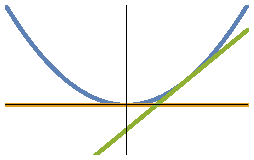
\includegraphics[width=\linewidth]{figures/parabola-linearizations.pdf}}
\noindent\hyperref[fig:parabola-linearizations]{右图}画出了这两个线性化, 与我们从微积分得到的直观认识一致.
\end{Example}

\begin{Example}{球面的线性化}\leavevmode\label{ex:linearizations-of-sphere}
考虑球面 $Y=\mathcal{V}(x^{2}+y^{2}+z^{2}-1)\subseteq\mathbb{A}^{3}_{\mathbb{C}}$, 其 $\mathcal{I}(Y)$ 由 $g=x^{2}+y^{2}+z^{2}-1$ 生成. 为计算在 $a=(0,0,-1)\in Y$ 处的线性化, 先计算生成元的线性化:
\[
  L_{a}g=0(x-0)+0(y-0)+(-2)(z+1)=-2(z+1).
\]
可见 $L_{a}Y=\mathcal{V}(-2(z+1))=\mathcal{V}(z+1)$, 它是包含 $a$ 且平行于 $xy$ 平面的平面.

\BookPairedFigure
  {另一方面, 若考虑点 $b=(1/\sqrt{3},1/\sqrt{3},1/\sqrt{3})\in Y$, 则生成元的线性化为
  \[
    L_{b}g=\frac{2}{\sqrt{3}}\bigl(x+y+z-\sqrt{3}\bigr).
  \]
  因此
  \[
    L_{b}Y=\mathcal{V}\bigl(x+y+z-\sqrt{3}\bigr).
  \]}
  {\phantomsection\label{fig:sphere-linearizations}%
   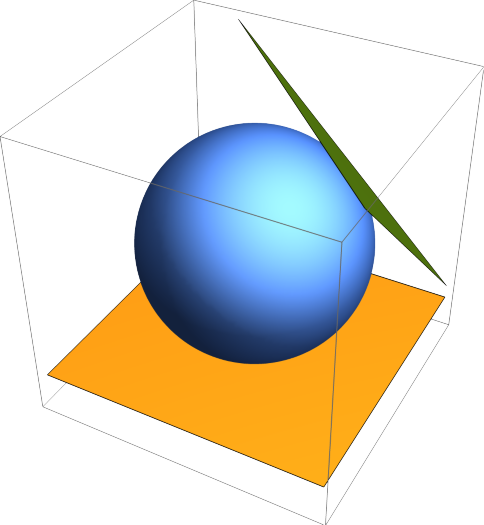
\includegraphics[width=\linewidth]{figures/sphere-linearizations.png}}
\noindent\hyperref[fig:sphere-linearizations]{图中}画出了实数域上的这些线性化, 它们同样符合微积分给出的直观认识.
\end{Example}

\begin{Example}{尖点曲线的线性化}\leavevmode\label{ex:linearizations-of-cusp}
\BookPairedFigure
  {考虑簇 $X=\mathcal{V}(x^{2}-y^{3})\subseteq\mathbb{A}^{2}$, \hyperref[fig:cusp-linearization]{右图}画出它在 $\mathbb{R}$ 上的图形. 如图可见, 这条曲线在原点处有一个\textquotedbl{}尖点\textquotedbl{}, 而在其他各点看上去都\textquotedbl{}光滑\textquotedbl{}. 这一几何观察反映在线性化上.}
  {\phantomsection\label{fig:cusp-linearization}%
   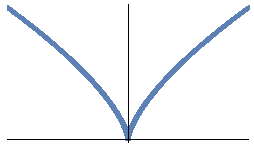
\includegraphics[width=\linewidth]{figures/cusp-linearization.pdf}}
建议读者在 Exercise~\ref{ex:linearizations-of-cusp-at-origin-and-elsewhere} 中验证: $X$ 在原点处的线性化是二维的 (整个 $\mathbb{A}^{2}$), 而在其余任一点处的线性化都是一维的. 在第~\ref{sec:smooth-and-singular-points}~节将看到, 线性化的维数可以用来识别簇中的\textquotedbl{}奇异\textquotedbl{}点, 例如 $X$ 的尖点.
\end{Example}

现在用线性化的概念来定义切空间.

\begin{Definition}{一点处的切向量和切空间}\leavevmode\label{def:tangent-vector-and-tangent-space}
设 $X\subseteq\mathbb{A}^{n}$ 为仿射簇, 且 $a=(a_{1},\ldots,a_{n})\in X$. 对任意 $b=(b_{1},\ldots,b_{n})\in L_{a}X$, 与 $b$ 对应的\emph{切向量}定义为
\[
  \overrightarrow{ab}=(b_{1}-a_{1},\ldots,b_{n}-a_{n})\in K^{n}.
\]
$X$ 在 $a$ 处的\emph{切空间}是所有切向量的集合:
\[
  T_{a}X=\{\overrightarrow{ab}\mid b\in L_{a}X\}\subseteq K^{n}.
\]
\end{Definition}

\BookPairedFigure
  {通常在几何上把切向量 $\overrightarrow{ab}$ 看成在线性化 $L_{a}X$ 内从 $a$ 指向 $b$ 的箭头. 回到 Example~\ref{ex:linearizations-of-sphere} 的单位球面, 取 $a=(0,0,-1)$, 就可以画出一些切向量, 如\hyperref[fig:sphere-tangent-vectors]{右图}所示.

  读到这里, 读者或许 (有理由) 分不清 $L_{a}X$ 和 $T_{a}X$, 这两个对象很相似. 事实上, 自然映射
  \[
    \begin{aligned}
      L_{a}X&\to T_{a}X,\\
      b&\mapsto\overrightarrow{ab}
    \end{aligned}
  \]
  是一个双射, 将 $L_{a}X$ 和 $T_{a}X$ 作为集合认同.}
  {\phantomsection\label{fig:sphere-tangent-vectors}%
   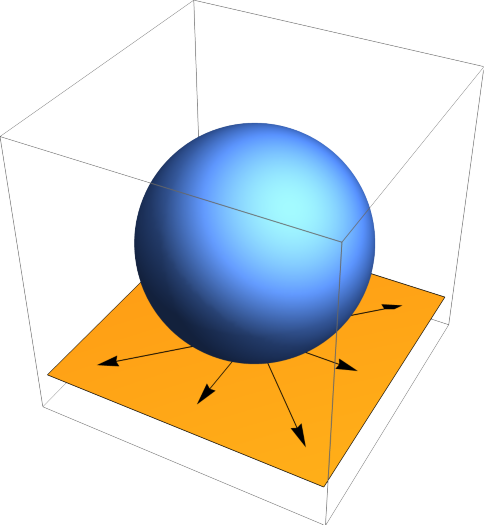
\includegraphics[width=\linewidth]{figures/sphere-tangent-vectors.png}}
那么, 为什么要给这两个相似的对象不同的名称和记号? 原因是我们把 $L_{a}X$ 看成几何对象, 即由 $\mathbb{A}^{n}$ 中的点组成的仿射簇; 而把 $T_{a}X$ 看成代数对象, 由 $K^{n}$ 中的向量组成. 事实上, 如下所见, 集合 $T_{a}X$ 是 $K^{n}$ 的向量子空间. 有了这一关键事实, 就能使用线性代数中的标准工具研究切空间.

在讨论为何切空间是 $K^{n}$ 的向量子空间之前, 先用梯度向量对 $T_{a}X$ 作一个有用的重新解释.

\begin{Definition}{梯度向量}\leavevmode\label{def:gradient-vector}
对任意 $a\in\mathbb{A}^{n}$ 和 $f\in K[x_{1},\ldots,x_{n}]$, $f$ 在 $a$ 处的\emph{梯度}是向量
\[
  \nabla f(a)=\left(\frac{\partial f}{\partial x_{1}}(a),\ldots,
    \frac{\partial f}{\partial x_{n}}(a)\right)\in K^{n}.
\]
\end{Definition}

下面的结论用梯度向量刻画切空间, 这与多元微积分中通常计算切平面的方式类似.

\begin{Proposition}{切空间的梯度刻画}\leavevmode\label{prop:gradient-characterization-of-tangent-spaces}
设 $X\subseteq\mathbb{A}^{n}$ 为仿射簇, 且 $a\in X$. 则
\[
  T_{a}X=\{v\in K^{n}\mid\nabla f(a)\cdot v=0\text{ 对所有 }f\in\mathcal{I}(X)\}.
\]
\end{Proposition}
\begin{Proof}
\BookPairedNoteLeft
  {设 $v=(v_{1},\ldots,v_{n})\in K^{n}$. 由 $T_{a}X$ 的定义可知, $v\in T_{a}X$ 当且仅当对某个 $b\in L_{a}X$, 有 $v=\overrightarrow{ab}$. 展开这个条件, 可知它等价于 $b=(v_{1}+a_{1},\ldots,v_{n}+a_{n})\in L_{a}X$.}
  {Proposition~\ref{prop:gradient-characterization-of-tangent-spaces} 中的\textquotedbl{}$\cdot$\textquotedbl{}是标准点积.}
由 $L_{a}X$ 的定义, $b\in L_{a}X$ 当且仅当对所有 $f\in\mathcal{I}(X)$ 都有
\[
  0=L_{a}f(b)=\sum_{i=1}^{n}\left[\frac{\partial f}{\partial x_{i}}(a)\right](b_{i}-a_{i})
    =\nabla f(a)\cdot v.
\]
因此 $v\in T_{a}X$ 当且仅当对所有 $f\in\mathcal{I}(X)$ 都有 $\nabla f(a)\cdot v=0$.
\end{Proof}

与 $L_{a}X$ 的情形一样, 建议读者验证: 若有一组有限生成元 $\mathcal{I}(X)=\langle f_{1},\ldots,f_{m}\rangle$, 则 Proposition~\ref{prop:gradient-characterization-of-tangent-spaces} 中的消失条件只须在生成元上检查:
\[
  T_{a}X=\{v\in K^{n}\mid\nabla f_{i}(a)\cdot v=0\text{ 对所有 }i=1,\ldots,m\}.
\]
作为 Proposition~\ref{prop:gradient-characterization-of-tangent-spaces} 的推论, 现在证明 $T_{a}X$ 是向量空间.

\begin{Corollary}{切空间是向量空间}\leavevmode\label{cor:tangent-space-is-vector-space}
设 $X\subseteq\mathbb{A}^{n}$ 为仿射簇, 且 $a\in X$. 切空间 $T_{a}X$ 是 $K^{n}$ 的一个向量子空间.
\end{Corollary}
\begin{Proof}
首先, $0\in T_{a}X$, 所以要验证 $T_{a}X$ 是子空间, 只需检查它对这些运算封闭. 设 $v,w\in T_{a}X$ 且 $r\in K$, 须验证 $v-rw\in T_{a}X$. 对任意 $f\in\mathcal{I}(X)$, 有
\[
  \nabla f(a)\cdot(v-rw)=\nabla f(a)\cdot v-r\nabla f(a)\cdot w=0,
\]
其中第一个等号来自点积的线性性, 第二个等号来自 Proposition~\ref{prop:gradient-characterization-of-tangent-spaces} 及假设 $v,w\in T_{a}X$. 因此由 Proposition~\ref{prop:gradient-characterization-of-tangent-spaces} 可知 $v+rw\in T_{a}X$, 证明完毕.
\end{Proof}

从仿射簇 $X\subseteq\mathbb{A}^{n}$ 及点 $a\in X$ 出发, 我们已经定义了向量空间 $T_{a}X\subseteq K^{n}$. 然而, 上面给出的 $T_{a}X$ 的定义是外在的: 它很大程度上依赖于包含关系 $X\subseteq\mathbb{A}^{n}$. 在第~\ref{sec:intrinsic-tangent-spaces}~节, 我们的主要目标是给出 $T_{a}X$ 的内在刻画, 它只依赖于 $K$-代数 $K[X]$ 和极大理想 $I_{a}\subseteq K[X]$, 后者由 $X$ 上在 $a$ 处为零的多项式函数组成. 这个刻画要用到线性代数中的对偶向量空间概念. 因此, 下一节须先稍作迂回, 讨论向量空间的对偶.

\BookExerciseHeading
\begin{BookExercises}
  \item\label{ex:linearization-and-tangency-from-generators} 设 $X\subseteq\mathbb{A}^{n}$ 为仿射簇, $a\in X$, 且 $\mathcal{I}(X)=\langle f_{1},\ldots,f_{m}\rangle$.
  \begin{enumerate}
    \item 证明
    \[
      L_{a}X=\mathcal{V}(L_{a}f_{1},\ldots,L_{a}f_{m}).
    \]
    \item 证明
    \[
      T_{a}X=\{v\in K^{n}\mid\nabla f_{i}(a)\cdot v=0\text{ 对所有 }i=1,\ldots,m\}.
    \]
  \end{enumerate}
  \item\label{ex:defining-polynomial-insufficient-for-linearization} 举出一个仿射簇 $X=\mathcal{V}(f)\subseteq\mathbb{A}^{n}$ 的例子, 使得
  \[
    L_{a}X\neq\mathcal{V}(L_{a}f).
  \]
  换句话说, 计算线性化时仅用定义多项式不够, 而需要用消没理想的生成元.
  \item\label{ex:linearizations-of-cusp-at-origin-and-elsewhere} 设 $X=\mathcal{V}(x^{2}-y^{3})\subseteq\mathbb{A}^{2}$. 证明原点 $(0,0)$ 处的线性化是二维的, 而在其余任一点处的线性化都是一维的.
  \item\label{ex:compare-linearizations-of-paraboloid} 设 $X=\mathcal{V}(x^{2}+y^{2}-z)\subseteq\mathbb{A}^{3}$.
  \begin{enumerate}
    \item 画出 $X$ 在 $\mathbb{R}$ 上的图形.
    \item 证明在 $(0,0,0)$ 处的线性化是三维的, 而在 $X$ 的其余任一点处的线性化都是二维的.
  \end{enumerate}
  \item\label{ex:tangent-space-and-linearization-have-equal-dimension} 对任意仿射簇 $X\subseteq\mathbb{A}^{n}$ 及 $a\in X$, 证明
  \[
    \dim(T_{a}X)=\dim(L_{a}X),
  \]
  其中左边是作为向量空间的维数, 右边是作为仿射簇的维数.
\end{BookExercises}

\par\medskip
{\footnotesize
\noindent\textbf{开放获取.} 本章按照
\href{http://creativecommons.org/licenses/by-nc/4.0/}{Creative Commons Attribution-NonCommercial 4.0 International License}
的条款授权. 该许可允许以任何媒介或格式进行非商业性使用, 分享, 改编, 分发和复制, 但须对原作者和来源作适当署名, 提供 Creative Commons 许可的链接, 并说明是否作了修改.

\noindent
\begin{minipage}[t]{.17\linewidth}
  \vspace{0pt}
\includegraphics[width=.9\linewidth]{figures/source-cc-by-nc.png}
\end{minipage}\hfill
\begin{minipage}[t]{.81\linewidth}
  \vspace{0pt}本章的图片或其他第三方材料均纳入本章的 Creative Commons 许可, 除非材料的署名行另有注明. 如果材料未纳入本章的 Creative Commons 许可, 且您拟进行的使用未获法律规定的许可或超出允许使用的范围, 则须直接向著作权持有人取得许可.
\end{minipage}\par}

\section{向量空间的对偶}\label{sec:vector-space-duality}

本节介绍从内在角度研究切空间所需的向量空间对偶的关键概念. 讨论最后将得到一个性质: 每个有限维向量空间都与它的双重对偶典范同构.

先定义向量空间的对偶. 它由该向量空间到基域的所有线性映射组成.

\begin{Definition}{向量空间的对偶}\leavevmode\label{def:dual-vector-space}
设 $V$ 为向量空间. $V$ 的\emph{对偶}记为 $V^{\vee}$, 是所有线性函数 $\phi:V\to K$ 的集合.
\end{Definition}

注意, 在到基域 $K$ 的函数通常的加法和标量乘法下, $V^{\vee}$ 本身也是向量空间 (Exercise~\ref{ex:dual-is-vector-space}). 此外, 给定 $V$ 的一组基, $V^{\vee}$ 上有一组自然的\textquotedbl{}对偶\textquotedbl{}基. 下面的定义基于这一事实: 任意线性函数 $V\to K$ 由它在 $V$ 的一组基的各元素上的取值唯一确定.

\begin{Definition}{一组基的对偶}\leavevmode\label{def:dual-of-a-basis}
若 $V$ 为有限维向量空间, 基 $\{v_{1},\ldots,v_{n}\}$ 的大小为 $n$, 则 $\{v_{1},\ldots,v_{n}\}$ 的\emph{对偶}是函数集 $\{v_{1}^{\vee},\ldots,v_{n}^{\vee}\}\subseteq V^{\vee}$, 它由下式确定:
\[
  v_{i}^{\vee}(v_{j})=
  \begin{cases}
    1 & i=j,\\
    0 & i\neq j.
  \end{cases}
\]
\end{Definition}

来看一个具体例子.

\begin{Example}{$K^{2}$ 的一组基的对偶}\leavevmode\label{ex:dual-of-a-basis-of-k-squared}
设 $V=K^{2}$, 考虑由以下两个向量组成的基:
\[
  v_{1}=(1,1),\qquad v_{2}=(1,-1).
\]
注意 $v_{1}^{\vee}:V\to K$ 将 $(1,1)$ 映到 $1$, 将 $(1,-1)$ 映到 $0$, 而 $v_{2}^{\vee}$ 将 $(1,1)$ 映到 $0$, 将 $(1,-1)$ 映到 $1$. 因此, 给定任意 $(a,b)\in K^{2}$, 写成
\[
  (a,b)=\frac{a+b}{2}(1,1)+\frac{a-b}{2}(1,-1)
\]
便得到
\[
  v_{1}^{\vee}(a,b)=\frac{a+b}{2}
  \qquad\text{和}\qquad
  v_{2}^{\vee}(a,b)=\frac{a-b}{2}.
\]
\end{Example}

正如可以预期的那样, $V$ 的一组基的对偶是 $V^{\vee}$ 的一组基. 现在验证这一点.

\begin{Proposition}{一组基的对偶是一组基}\leavevmode\label{prop:dual-basis-is-a-basis}
若向量空间 $V$ 有一组大小为 $n$ 的基 $\{v_{1},\ldots,v_{n}\}$, 则 $\{v_{1}^{\vee},\ldots,v_{n}^{\vee}\}$ 是 $V^{\vee}$ 的一组基.
\end{Proposition}
\begin{Proof}
证明 $\{v_{1}^{\vee},\ldots,v_{n}^{\vee}\}$ 线性独立且张成 $V^{\vee}$.

为证明线性独立, 设对某些 $a_{1},\ldots,a_{n}\in K$, 有 $a_{1}v_{1}^{\vee}+\cdots+a_{n}v_{n}^{\vee}=0$. 在 $v_{i}$ 处取值, 得
\[
  0=(a_{1}v_{1}^{\vee}+\cdots+a_{n}v_{n}^{\vee})(v_{i})=a_{i}.
\]
因此 $a_{1}=\cdots=a_{n}=0$, 这说明 $\{v_{1}^{\vee},\ldots,v_{n}^{\vee}\}$ 线性独立.

为证明 $\{v_{1}^{\vee},\ldots,v_{n}^{\vee}\}$ 张成 $V^{\vee}$, 设 $\phi\in V^{\vee}$, 即 $\phi:V\to K$ 为线性函数. 考虑线性组合 $\phi(v_{1})v_{1}^{\vee}+\cdots+\phi(v_{n})v_{n}^{\vee}$. 注意对每个 $j=1,\ldots,n$, 由 $v_{1}^{\vee},\ldots,v_{n}^{\vee}$ 的定义有
\[
  (\phi(v_{1})v_{1}^{\vee}+\cdots+\phi(v_{n})v_{n}^{\vee})(v_{j})=\phi(v_{j}).
\]
由于 $\{v_{1},\ldots,v_{n}\}$ 是 $V$ 的一组基, 且线性函数 $\phi(v_{1})v_{1}^{\vee}+\cdots+\phi(v_{n})v_{n}^{\vee}$ 和 $\phi$ 在每个基元素上相同, 可知 $\phi=\phi(v_{1})v_{1}^{\vee}+\cdots+\phi(v_{n})v_{n}^{\vee}$. 由于 $\phi$ 是任意的, 这说明 $\{v_{1}^{\vee},\ldots,v_{n}^{\vee}\}$ 张成 $V^{\vee}$.
\end{Proof}

\BookPairedNote
  {前一个结论蕴含, 有限维向量空间的对偶本身也是同维的有限维向量空间. 特别地, 给定 $V$ 的一组基, 就有一个同构 $V\cong V^{\vee}$, 它将每个基元素映到相应的对偶基元素.}
  {注意 Proposition~\ref{prop:dual-basis-is-a-basis} 对无限维向量空间不成立, 见 Exercise~\ref{ex:infinite-dimensional-dual-basis-failure}.}
由此产生一个重要问题: 这个同构是否与基无关? 答案是\textquotedbl{}否\textquotedbl{}, 如下例所示.

\begin{Example}{不同的基定义不同的同构 $V\cong V^{\vee}$}\leavevmode\label{ex:duality-isomorphisms-depend-on-basis}
设 $V=K^{2}$, 考虑分别由下面两对元素给出的两组基:
\[
  v_{1}=(1,0),\quad v_{2}=(0,1)
  \qquad\text{和}\qquad
  w_{1}=(1,0),\quad w_{2}=(1,1).
\]
可以验证 $\{v_{1},v_{2}\}$ 的对偶基由
\[
  v_{1}^{\vee}(a,b)=a\qquad\text{和}\qquad v_{2}^{\vee}(a,b)=b
\]
给出, 而 $\{w_{1},w_{2}\}$ 的对偶基由
\[
  w_{1}^{\vee}(a,b)=a-b\qquad\text{和}\qquad w_{2}^{\vee}(a,b)=b
\]
给出. 特别地, 由于 $v_{1}=w_{1}$ 但 $v_{1}^{\vee}\neq w_{1}^{\vee}$, 可知把 $v_{1},v_{2}$ 映到 $v_{1}^{\vee},v_{2}^{\vee}$ 的 $V$ 与 $V^{\vee}$ 之间的同构, 不同于把 $w_{1},w_{2}$ 映到 $w_{1}^{\vee},w_{2}^{\vee}$ 的同构.
\end{Example}

我们已经看到如何选择一组基来构造 $V$ 与 $V^{\vee}$ 之间的同构. 但前例表明, 对不同的基, 这些同构通常不同. 事实上, 无论怎么尝试, 如果不作一些额外选择 (比如选定一组基), 就无法构造非零向量空间与其对偶之间的同构.

\BookPairedNote
  {那么, 以下事实或许有点出人意料: 再取一次对偶, 就会发现 $V$ 与 $(V^{\vee})^{\vee}$ 之间存在典范同构.}
  {通常称 $(V^{\vee})^{\vee}$ 为 $V$ 的\textquotedbl{}双重对偶\textquotedbl{}.}

\begin{Theorem}{$V=(V^{\vee})^{\vee}$}\leavevmode\label{thm:vector-space-canonically-isomorphic-to-double-dual}
若 $V$ 是有限维向量空间, 则 $V$ 与 $(V^{\vee})^{\vee}$ 之间存在典范同构.
\end{Theorem}
\begin{Proof}
定义 $\omega:V\to(V^{\vee})^{\vee}$, 把 $V$ 中向量 $v$ 送到 $V^{\vee}$ 上相应的\textquotedbl{}取值函数\textquotedbl{}, 其定义为
\[
  \begin{aligned}
    e_{v}:V^{\vee}&\to K,\\
    \phi&\mapsto\phi(v).
  \end{aligned}
\]
稍加思考即可看出, 对任意 $a\in K$ 及 $v,w\in V$, 有 $e_{av+w}=ae_{v}+e_{w}$. 换句话说, $\omega$ 是线性映射. 注意, 线性映射 $\omega$ 的确是典范地定义的, 因为其定义不需要任何额外选择 (比如选择一组基).

还须证明 $\omega$ 是同构, 为此选取一组基. 设 $V$ 的维数为 $n$, 且 $\{v_{1},\ldots,v_{n}\}\subseteq V$ 为 $V$ 的一组基. 在对偶基元素 $v_{j}^{\vee}\in V^{\vee}$ 处对取值函数 $e_{v_{i}}$ 取值, 得
\[
  e_{v_{i}}(v_{j}^{\vee})=v_{j}^{\vee}(v_{i})=
  \begin{cases}
    1 & i=j,\\
    0 & i\neq j.
  \end{cases}
\]
换句话说, 这表明 $\{e_{v_{1}},\ldots,e_{v_{n}}\}$ 是对偶基 $\{v_{1}^{\vee},\ldots,v_{n}^{\vee}\}$ 的对偶基, 因而由 Lemma~\ref{prop:dual-basis-is-a-basis} 可知它是一组基. 由于 $\omega$ 是把 $V$ 的一组基送到 $(V^{\vee})^{\vee}$ 的一组基的线性映射, 由标准的线性代数论证得 $\omega$ 是同构.
\end{Proof}

\BookPairedNoteLeft
  {熟悉了向量空间的对偶 (和双重对偶) 后, 下一节回到切空间的话题. 那里将给出切空间的一种内在描述, 它不依赖于仿射簇置于仿射空间中的方式.}
  {注意, 对任意向量空间 $V$, $\omega:V\to(V^{\vee})^{\vee}$ 都是单射, 但只有在 $\dim(V)<\infty$ 时才是满射.}

\BookExerciseHeading
\begin{BookExercises}
  \item\label{ex:dual-is-vector-space} 设 $V$ 为向量空间. 证明 $V^{\vee}$ 也是向量空间.
  \item\label{ex:distinct-bases-may-give-same-duality-isomorphism} 给出 $K^{2}$ 的两组不同的基 $\{v_{1},v_{2}\}$ 和 $\{w_{1},w_{2}\}$, 使得由 $v_{i}\mapsto v_{i}^{\vee}$ 和 $w_{i}\mapsto w_{i}^{\vee}$ 给出的同构 $V\to V^{\vee}$ 相同.
  \item\label{ex:infinite-dimensional-dual-basis-failure} 考虑无限维向量空间 $K[x]$ 及其基 $\{1,x,x^{2},x^{3},\ldots\}$. 证明线性映射
  \[
    \begin{aligned}
      K[x]&\to K,\\
      f&\mapsto f(1)
    \end{aligned}
  \]
  不在 $1^{\vee},x^{\vee},(x^{2})^{\vee},(x^{3})^{\vee},\ldots$ 的张成空间中.
  \item\label{ex:linear-maps-from-base-field} 设 $V$ 为向量空间, $W$ 为线性映射 $K\to V$ 的集合. 证明 $V$ 和 $W$ 是典范同构的向量空间.
  \item\label{ex:linear-maps-into-finite-dimensional-vector-space} 设 $V$ 和 $W$ 为向量空间, $W$ 的有限维数为 $n$, 且 $\{w_{1},\ldots,w_{n}\}$ 为 $W$ 的一组基. 构造 $(V^{\vee})^{n}$ 与线性映射 $V\to W$ 所成向量空间之间的一个同构.
  \item\label{ex:dual-and-double-dual-of-linear-map} 设 $V$ 和 $W$ 为向量空间. 给定线性映射 $\phi:V\to W$, 定义 $\phi$ 的\emph{对偶}为
  \[
    \begin{aligned}
      \phi^{\vee}:W^{\vee}&\to V^{\vee},\\
      \psi&\mapsto\psi\circ\phi.
    \end{aligned}
  \]
  \begin{enumerate}
    \item 说明对任意线性映射 $\phi:V\to W$ 和 $\psi\in W^{\vee}$, 为什么有 $\psi\circ\phi\in V^{\vee}$.
    \item 证明 $\phi^{\vee}$ 是线性映射.
    \item 设 $V$ 和 $W$ 均为有限维. 证明 $(\phi^{\vee})^{\vee}=\phi$.
  \end{enumerate}
\end{BookExercises}

\section{从坐标环得到切空间}\label{sec:intrinsic-tangent-spaces}

本节的目标是完全用坐标环 $K[X]$ 重新解释切空间 $T_{a}X$. 这一内在描述的一个有用推论是, 切空间在同构下保持不变. 换句话说, 若 $F:X\to Y$ 为同构, 且 $a\in X$, 则 $T_{a}X$ 和 $T_{F(a)}Y$ 是同构的向量空间.

为了开始给出切空间的内在描述, 首先需要一种内在的方式来理解点 $a\in X$. 给定 $a\in X$, 定义
\[
  I_{a}=\{F\in K[X]\mid F(a)=0\}\subseteq K[X].
\]
由定义可见, $I_{a}$ 是 $K[X]$ 的子集. 不止如此, $I_{a}$ 是 $K[X]$ 的极大理想, 建议读者在 Exercise~\ref{ex:point-ideal-is-maximal-in-coordinate-ring} 中验证. 注意 $I_{a}$ 是内在定义的, 不涉及 $X$ 所处的环境仿射空间.

为更具体地描述 $I_{a}$, 考虑 $K[X]$ 的一种 (外在的) 商环描述. 更具体地说, 假设 $X\subseteq\mathbb{A}^{n}$, 于是可写 $K[X]=K[x_{1},\ldots,x_{n}]/\mathcal{I}(X)$ 和 $a=(a_{1},\ldots,a_{n})\in X$. 对任意 $F\in K[X]$, 可对某个 $f\in K[x_{1},\ldots,x_{n}]$ 写作 $F=[f]$. 那么 $F\in I_{a}$ 当且仅当 $f(a)=0$. 因为每个在 $a$ 处取值为零的多项式都能写为
\[
  f=(x_{1}-a_{1})f_{1}+\cdots+(x_{n}-a_{n})f_{n},
\]
其中 $f_{1},\ldots,f_{n}\in K[x_{1},\ldots,x_{n}]$ 为某些多项式, 所以
\begin{equation}\label{eq:point-ideal-from-coordinate-generators}
  I_{a}=\langle[x_{1}-a_{1}],\ldots,[x_{n}-a_{n}]\rangle
    \subseteq\frac{K[x_{1},\ldots,x_{n}]}{\mathcal{I}(X)}.
\end{equation}
注意, $I_{a}$ 可以自然地看成向量空间: 两个在 $a$ 处取值为零的函数之和在 $a$ 处取值为零, 一个在 $a$ 处取值为零的函数乘以标量后也在 $a$ 处取值为零.

现在考虑理想 $I_{a}^{2}=I_{a}\cdot I_{a}$, 即 $I_{a}$ 与自身的理想乘积. 利用等式 \eqref{eq:point-ideal-from-coordinate-generators} 中 $I_{a}$ 的生成元, 可得
\begin{equation}\label{eq:square-of-point-ideal}
  I_{a}^{2}=\langle[(x_{i}-a_{i})(x_{j}-a_{j})]\mid1\leq i,j\leq n\rangle\subseteq I_{a}.
\end{equation}
注意 $I_{a}^{2}$ 是 $I_{a}$ 的向量子空间, 所以可以考虑商向量空间 $I_{a}/I_{a}^{2}$. 用等式 \eqref{eq:point-ideal-from-coordinate-generators} 中的生成元来看, 该商是有限维的, 由线性函数 $[x_{i}-a_{i}]$ 张成 (Exercise~\ref{ex:point-ideal-quotient-spanned-by-coordinate-linear-functions}):
\[
  I_{a}/I_{a}^{2}=K\{[x_{1}-a_{1}],\ldots,[x_{n}-a_{n}]\}.
\]
本节的主要结论如下, 它将有限维向量空间 $I_{a}/I_{a}^{2}$ 解释为切空间 $T_{a}X$ 的对偶.

\begin{Theorem}{$I_{a}/I_{a}^{2}=(T_{a}X)^{\vee}$}\leavevmode\label{thm:point-ideal-square-quotient-is-dual-of-tangent-space}
设 $X\subseteq\mathbb{A}^{n}$ 为仿射簇, 且 $a\in X$. 则有典范的向量空间同构
\[
  I_{a}/I_{a}^{2}=(T_{a}X)^{\vee}.
\]
\end{Theorem}

在给出证明之前, 先考察几个熟悉的切空间例子, 以便理解 Theorem~\ref{thm:point-ideal-square-quotient-is-dual-of-tangent-space} 中的新概念.

\begin{Example}{抛物线的切空间}\leavevmode\label{ex:tangent-space-of-parabola}
考虑抛物线 $X=\mathcal{V}(y-x^{2})\subseteq\mathbb{A}^{2}$, 令 $a=(0,0)$. 在 Example~\ref{ex:linearizations-of-parabola} 中, 我们算出 $X$ 有一维线性化 $L_{a}X$, 因而切空间 $T_{a}X$ 是一维的. 由 Theorem~\ref{thm:point-ideal-square-quotient-is-dual-of-tangent-space}, 可知 $I_{a}/I_{a}^{2}$ 应为一维向量空间. 为直接验证这一点, 注意
\[
  \begin{aligned}
    I_{a}&=\langle[x],[y]\rangle\\
      &=K\{[x],[y],[x^{2}],[xy],[y^{2}],[x^{3}],[x^{2}y],[xy^{2}],[y^{3}],\ldots\}\subseteq K[X]
  \end{aligned}
\]
且
\[
  \begin{aligned}
    I_{a}^{2}&=\langle[x^{2}],[xy],[y^{2}]\rangle\\
      &=K\{[x^{2}],[xy],[y^{2}],[x^{3}],[x^{2}y],[xy^{2}],[y^{3}],\ldots\}\subseteq K[X].
  \end{aligned}
\]
注意到在 $K[X]$ 中 $[y]=[x^{2}]$, 可知除 $[x]$ 之外, $I_{a}$ 的上述每个生成元也出现在 $I_{a}^{2}$ 中. 所以 $I_{a}/I_{a}^{2}=K\{[x]\}$, 这如预期是 $K$ 上的一维向量空间. 此外, 函数 $[x]\in K[X]$ 在线性化 $L_{a}X=\mathcal{V}(y)\subseteq\mathbb{A}^{2}$ 上给出线性函数. 将 $L_{a}X=\{(a,0)\mid a\in K\}$ 与 $T_{a}X=K$ 认同后, 就可以自然地将向量空间 $I_{a}/I_{a}^{2}=K\{[x]\}$ 与对偶空间 $(T_{a}X)^{\vee}$ 认同.
\end{Example}

\begin{Example}{尖点曲线的切空间}\leavevmode\label{ex:tangent-space-of-cusp}
如 Example~\ref{ex:linearizations-of-cusp}, 考虑尖点曲线 $X=\mathcal{V}(x^{2}-y^{3})\subseteq\mathbb{A}^{2}$, 令 $a=(0,0)$. 在 Exercise~\ref{ex:linearizations-of-cusp-at-origin-and-elsewhere} 中, 建议读者证明 $X$ 有二维线性化 $L_{a}X=\mathbb{A}^{2}$, 从而有二维切空间 $T_{a}X=K^{2}$. 由 Theorem~\ref{thm:point-ideal-square-quotient-is-dual-of-tangent-space} 可知 $I_{a}/I_{a}^{2}$ 应是二维向量空间.

为直接验证这一预期, 完全按上一例计算 $I_{a}$ 和 $I_{a}^{2}$. 但与上一例不同的是, $[x]$ 和 $[y]$ 在商 $I_{a}/I_{a}^{2}$ 中仍然线性独立. 所以 $I_{a}/I_{a}^{2}=K\{[x],[y]\}$ 是二维向量空间. 将 $L_{a}X=\mathbb{A}^{2}$ 与 $T_{a}X=K^{2}$ 认同后, 可以自然地将向量空间 $I_{a}/I_{a}^{2}=K\{[x],[y]\}$ 看作对偶空间 $(T_{a}X)^{\vee}$.
\end{Example}

\begin{Proof}\textbf{of Theorem~\ref{thm:point-ideal-square-quotient-is-dual-of-tangent-space}.}\quad
我们定义典范的满射线性映射
\[
  \phi:I_{a}\to(T_{a}X)^{\vee}
\]
并证明 $\ker(\phi)=I_{a}^{2}$. 为定义 $\phi$, 设 $F\in I_{a}$, 并对某个 $f\in K[x_{1},\ldots,x_{n}]$ 写作 $F=[f]$. 定义 $\phi(F)$ 为线性映射
\[
  \begin{aligned}
    \phi(F):T_{a}X&\to K,\\
    v&\mapsto\nabla f(a)\cdot v.
  \end{aligned}
\]
当然, 我们应当顾虑这一定义是否依赖于代表元 $f$ 的选择. 然而, 由 Proposition~\ref{prop:gradient-characterization-of-tangent-spaces} 可知 (Exercise~\ref{ex:tangent-functional-independent-of-representative})
\[
  [f]=[g]\quad\Longrightarrow\quad
  \nabla f(a)\cdot v=\nabla g(a)\cdot v\qquad\text{对所有 }v\in T_{a}X,
\]
所以 $\phi(F)\in(T_{a}X)^{\vee}$ 与代表元 $f$ 的选择无关. 验证 $\phi$ 的线性性, 要求对任意 $F,G\in K[X]$ 和 $r\in K$ 都有 $\phi(F+rG)=\phi(F)+r\phi(G)$. 这由求导的线性性得到 (Exercise~\ref{ex:map-from-point-ideal-to-tangent-dual-is-linear}). 所以只剩证明 $\phi$ 是满射且 $\ker(\phi)=I_{a}^{2}$.

为证明 $\phi$ 是满射, 设 $\rho:T_{a}X\to K$ 为线性映射, 并将它扩张为线性映射 $\overline{\rho}:K^{n}\to K$. 定义线性多项式
\[
  f=\overline{\rho}(e_{1})(x_{1}-a_{1})+\cdots+\overline{\rho}(e_{n})(x_{n}-a_{n})
    \in K[x_{1},\ldots,x_{n}],
\]
其中 $e_{1},\ldots,e_{n}$ 是 $K^{n}$ 的标准基向量, 并注意 $[f]\in I_{a}$. 我们断言 $\phi([f])=\rho$. 将定义展开, 可见对所有 $i=1,\ldots,n$, 有 $\nabla f(a)\cdot e_{i}=\overline{\rho}(e_{i})$. 由于 $T_{a}X\subseteq K^{n}$ 上的线性映射由任意一个扩张在标准基向量上的取值唯一确定, 对所有 $v\in T_{a}X$ 都有 $\nabla f(a)\cdot v=\rho(v)$, 所以 $\phi([f])=\rho$. 因此 $\phi$ 是满射.

为证明 $\ker(\phi)=I_{a}^{2}$, 先设 $F\in I_{a}^{2}$. 由等式 \eqref{eq:square-of-point-ideal}, 有 $F=[f]$, 其中 $f$ 的形式为
\[
  f=\sum_{i,j=1}^{n}(x_{i}-a_{i})(x_{j}-a_{j})f_{i,j}
  \qquad\text{其中 }f_{i,j}\in K[x_{1},\ldots,x_{n}].
\]
利用乘积法则求 $f$ 的导数, 得 $\nabla f(a)=0$, 从而 $F\in\ker(\phi)$. 因此 $I_{a}^{2}\subseteq\ker(\phi)$.

为证明反向包含, 设 $F\in\ker(\phi)$, 并对某个 $f\in K[x_{1},\ldots,x_{n}]$ 写作 $F=[f]$. 假设 $F\in\ker(\phi)$ 意味着
\[
  \nabla f(a)\cdot v=0\qquad\text{对所有 }v\in T_{a}X.
\]
选取生成元 $\mathcal{I}(X)=\langle g_{1},\ldots,g_{m}\rangle$, 则由 Proposition~\ref{prop:gradient-characterization-of-tangent-spaces} 和线性代数的论证 (Exercise~\ref{ex:annihilator-of-kernel-is-row-span}) 得
\[
  \nabla f(a)=\sum_{i=1}^{m}a_{i}\nabla g_{i}(a),
\]
其中 $a_{1},\ldots,a_{m}\in K$ 为某些标量. 由于梯度对多项式线性作用, 且 $\mathcal{I}(X)$ 对线性组合封闭, 可见
\[
  \nabla f(a)=\nabla g(a)\qquad\text{其中 }g=\sum_{i=1}^{m}a_{i}g_{i}\in\mathcal{I}(X).
\]
利用 $F=[f]$ 属于 $\phi$ 的定义域从而 $[f]\in I_{a}$, 可以写成
\[
  f=\sum_{i=1}^{n}b_{i}(x_{i}-a_{i})
    +\sum_{i,j=1}^{n}f_{i,j}(x_{i}-a_{i})(x_{j}-a_{j}).
\]
对 $g$ 写出类似的表达式, 则等式 $\nabla f(a)=(b_{1},\ldots,b_{n})=\nabla g(a)$ 蕴含
\[
  f-g=\sum_{i,j=1}^{n}(f_{i,j}-g_{i,j})(x_{i}-a_{i})(x_{j}-a_{j}).
\]
由于 $g\in\mathcal{I}(X)$, 有 $[f]=[f-g]$, 从上面的表达式得到
\[
  F=[f-g]\in\langle[(x_{i}-a_{i})(x_{j}-a_{j})]\mid1\leq i,j\leq n\rangle=I_{a}^{2},
\]
证明完毕.
\end{Proof}

对 Theorem~\ref{thm:point-ideal-square-quotient-is-dual-of-tangent-space} 中的两边取对偶, 并应用 Theorem~\ref{thm:vector-space-canonically-isomorphic-to-double-dual}, 得到切空间的以下内在刻画.

\begin{Corollary}{$T_{a}X=(I_{a}/I_{a}^{2})^{\vee}$}\leavevmode\label{cor:tangent-space-as-dual-of-point-ideal-quotient}
设 $X\subseteq\mathbb{A}^{n}$ 为仿射簇, 且 $a\in X$. 则有典范的向量空间同构
\[
  T_{a}X=(I_{a}/I_{a}^{2})^{\vee}.
\]
\end{Corollary}

Theorem~\ref{thm:point-ideal-square-quotient-is-dual-of-tangent-space} 和 Corollary~\ref{cor:tangent-space-as-dual-of-point-ideal-quotient} 的主要收获是, 现在研究仿射簇的切空间无需提及该簇所处的仿射空间. 更具体地说, 我们已经看到, 任意一点 $a\in X$ 对应于坐标环 $K[X]$ 中的一个极大理想 $I_{a}$, 现在只须将切空间 $T_{a}X$ 抽象地看成向量空间 $(I_{a}/I_{a}^{2})^{\vee}$ 来研究. 正如你可能猜到的那样, 切空间确实是内在的, 即它们在同构下保持不变. 本节最后明确说明切空间的这种内在性.

\begin{Corollary}{切空间是内在的}\leavevmode\label{cor:tangent-spaces-invariant-under-isomorphism}
设 $X$ 和 $Y$ 为仿射簇, $F:X\to Y$ 为同构, 且 $a\in X$. 则 $F$ 诱导向量空间同构
\[
  T_{a}X\cong T_{F(a)}Y.
\]
\end{Corollary}
\begin{Proof}
建议读者在 Exercise~\ref{ex:pullback-identifies-maximal-point-ideals} 中验证: 拉回同构 $F^{*}:K[Y]\to K[X]$ 将极大理想 $I_{F(a)}$ 与 $I_{a}$ 认同:
\[
  F^{*}(I_{F(a)})=I_{a}.
\]
由此得
\[
  F^{*}(I_{F(a)}^{2})=I_{a}^{2}.
\]
因而 $F^{*}$ 诱导向量空间同构 $I_{F(a)}/I_{F(a)}^{2}\cong I_{a}/I_{a}^{2}$, 取对偶即得同构 $T_{a}X\cong T_{F(a)}Y$.
\end{Proof}

\BookExerciseHeading
\begin{BookExercises}
  \item\label{ex:point-ideal-is-maximal-in-coordinate-ring} 设 $X$ 为仿射簇, $a\in X$ 为一点. 证明
  \[
    I_{a}=\{F\in K[X]\mid F(a)=0\}
  \]
  是 $K[X]$ 的极大理想.
  \item\label{ex:point-ideal-quotient-spanned-by-coordinate-linear-functions} 设 $X\subseteq\mathbb{A}^{n}$ 为仿射簇, 且 $a\in X$. 证明
  \[
    I_{a}/I_{a}^{2}=K\{[x_{1}-a_{1}],\ldots,[x_{n}-a_{n}]\}.
  \]
  \item\label{ex:tangent-functional-independent-of-representative} 设 $X\subseteq\mathbb{A}^{n}$ 为仿射簇, 且 $a\in X$. 证明若 $[f]=[g]\in K[X]$, 则对所有 $v\in T_{a}X$, 有 $\nabla f(a)\cdot v=\nabla g(a)\cdot v$.
  \item\label{ex:map-from-point-ideal-to-tangent-dual-is-linear} 设 $\phi$ 如 Theorem~\ref{thm:point-ideal-square-quotient-is-dual-of-tangent-space} 的证明中所定义. 对任意 $F,G\in K[X]$ 和 $r\in K$, 利用求导的线性性证明
  \[
    \phi(F+rG)=\phi(F)+r\phi(G).
  \]
  \item\label{ex:annihilator-of-kernel-is-row-span} 设 $v_{1},\ldots,v_{m}\in K^{n}$, 且 $V\subseteq K^{n}$ 是由下式给出的线性子空间:
  \[
    V=\{v\in K^{n}\mid v_{i}\cdot v=0\text{ 对所有 }i=1,\ldots,m\}.
  \]
  假设 $w\in K^{n}$ 对所有 $v\in V$ 都满足 $w\cdot v=0$. 证明 $w$ 属于 $v_{1},\ldots,v_{m}$ 的张成空间. (提示: 考虑以 $v_{1},\ldots,v_{m}$ 为各行的矩阵 $M$, 以及把行 $w$ 添加到 $M$ 得到的矩阵 $M'$. 用秩--零度论证证明 $\operatorname{rk}(M)=\operatorname{rk}(M')$.)
  \item\label{ex:pullback-identifies-maximal-point-ideals} 设 $X\subseteq\mathbb{A}^{m}$ 和 $Y\subseteq\mathbb{A}^{n}$ 为仿射簇, $F:X\to Y$ 为同构, 且 $a\in X$. 证明 $F^{*}:K[Y]\to K[X]$ 将极大理想 $I_{F(a)}$ 与 $I_{a}$ 认同:
  \[
    F^{*}(I_{F(a)})=I_{a}.
  \]
\end{BookExercises}

\section{切空间与维数}\label{sec:dimension-of-tangent-spaces}

在第~\ref{sec:linearizations-and-tangent-spaces}~节看到线性化和切空间的几个例子. 读者或许注意到, 切空间的维数有时大于簇本身的维数, 却从不小于它. 不可约簇的维数是该簇任一点处切空间维数的下界, 这就是本节的主要结论.

\begin{Proposition}{切空间维数的下界}\leavevmode\label{prop:tangent-dimension-lower-bound}
设 $X\subseteq\mathbb{A}^{n}$ 为不可约仿射簇, 且 $a\in X$. 则
\[
  \dim(T_{a}X)\geq\dim(X).
\]
\end{Proposition}

注意, 不等式左边的维数是 $T_{a}X\subseteq K^{n}$ 作为向量空间的维数, 右边的维数是 $X\subseteq\mathbb{A}^{n}$ 作为仿射簇的维数. 如果愿意, 可以将 Proposition~\ref{prop:tangent-dimension-lower-bound} 中不等式的两边都解释为 $\mathbb{A}^{n}$ 中仿射簇的维数, 只需注意 $\dim(T_{a}X)=\dim(L_{a}X)$ (Exercise~\ref{ex:tangent-space-and-linearization-have-equal-dimension}).

在证明 Proposition~\ref{prop:tangent-dimension-lower-bound} 之前, 先证明零维情形中一个更强的充要条件.

\begin{Lemma}{零维切空间}\leavevmode\label{lem:zero-dimensional-tangent-spaces}
若 $X\subseteq\mathbb{A}^{n}$ 为不可约仿射簇, 且 $a\in X$, 则 $\dim(X)=0$ 当且仅当 $\dim(T_{a}X)=0$.
\end{Lemma}
\begin{Proof}
若 $\dim(X)=0$, 则 $X$ 只含点 $a$. 由定义可验证 $T_{a}X=\{0\}$ (Exercise~\ref{ex:tangent-space-of-single-point}).

为证明反向, 假设 $\dim(T_{a}X)=0$, 并考虑由在 $a$ 处取值为零的多项式函数组成的极大理想 $I_{a}\subseteq K[X]$. 我们要证明 $I_{a}$ 是零理想. 这将推出 $K[X]$ 中的零理想是极大理想, 所以 $K[X]$ 是域, 再由零点定理推出 $X$ 只有一个点.

因为有限维向量空间与其对偶维数相同, Theorem~\ref{thm:point-ideal-square-quotient-is-dual-of-tangent-space} 与 $\dim(T_{a}X)=0$ 这一假设蕴含 $I_{a}=I_{a}^{2}$. 选取生成元
\[
  I_{a}=\langle F_{1},\ldots,F_{m}\rangle.
\]
由于 $I_{a}=I_{a}^{2}$, 可以把每个 $F_{i}$ 视为 $I_{a}^{2}$ 的元素, 从而可以找到形如
\[
  F_{i}=G_{i,1}F_{1}+\cdots+G_{i,m}F_{m}
\]
的等式, 其中对每个 $i,j=1,\ldots,m$, 有 $G_{i,j}\in I_{a}$. 于是得到线性方程组
\[
  (I-G)\cdot
  \begin{pmatrix}F_{1}\\\vdots\\F_{m}\end{pmatrix}
  =\begin{pmatrix}0\\\vdots\\0\end{pmatrix},
\]
其中 $I$ 为 $m\times m$ 单位矩阵, $G$ 是以 $G_{i,j}$ 为元素的矩阵.

应用 Cramer 法则, 得对所有 $i=1,\ldots,m$ 都有
\[
  \det(I-G)F_{i}=0\in K[X].
\]
注意 $\det(I-G)$ 是 $X$ 上的多项式函数, 又因为对所有 $i,j$ 都有 $G_{i,j}(a)=0$, 所以 $\det(I-G)$ 在 $a$ 处取值为 $1$. 因此 $\det(I-G)$ 不是 $X$ 上的零函数. 因为 $K[X]$ 是整环 (这里用到 $X$ 不可约的假设), 可知对所有 $i$ 都有 $F_{i}=0$. 所以 $I_{a}$ 是零理想, 证明完毕.
\end{Proof}

现在证明 Proposition~\ref{prop:tangent-dimension-lower-bound}. 证明对 $\dim(X)$ 归纳. 归纳步骤 (需要用到 Lemma~\ref{lem:zero-dimensional-tangent-spaces}) 通过用一个超平面, 即由单个线性方程定义的簇, 同时切割 $X$ 与 $L_{a}X$, 并应用维数论基本定理来完成.

\begin{Proof}\textbf{of Proposition~\ref{prop:tangent-dimension-lower-bound}.}\quad
给定不可约仿射簇 $X\subseteq\mathbb{A}^{n}$ 及点 $a\in X$, 对 $\dim(X)$ 归纳证明 $\dim(T_{a}X)\geq\dim(X)$.

(归纳起点) 若 $\dim(X)=0$, 则由向量空间的维数非负可知 $\dim(T_{a}X)\geq\dim(X)$. (实际上, 由 Lemma~\ref{lem:zero-dimensional-tangent-spaces} 还知道更多: 在这种情形下 $\dim(T_{a}X)=\dim(X)$.)

(归纳步骤) 设 $X\subseteq\mathbb{A}^{n}$ 为正维不可约仿射簇. 假设命题中的不等式对所有维数为 $\dim(X)-1$ 的不可约仿射簇成立. 令 $a=(a_{1},\ldots,a_{n})\in X$.

由于已假设 $\dim(X)>0$, Lemma~\ref{lem:zero-dimensional-tangent-spaces} 中\textquotedbl{}若\textquotedbl{}的方向蕴含 $T_{a}X\supsetneq\{0\}$, 这等价于 $L_{a}X\supsetneq\{a\}$. 因此可以选取一点 $b\in L_{a}X\setminus\{a\}$. 两点 $a,b\in\mathbb{A}^{n}$ 至少有一个坐标不同, 不妨设它们的第一个坐标不同, 并定义超平面
\[
  H=\mathcal{V}(x_{1}-a_{1})\subseteq\mathbb{A}^{n}.
\]
令 $Y=X\cap H$. 首先注意 $Y$ 不可能是整个 $X$. 事实上, 若 $Y=X$, 则 $X\subseteq H$, 这将蕴含 $L_{a}X\subseteq H$ (Exercise~\ref{ex:linearization-monotone-under-inclusion} 和~\ref{ex:linear-variety-equals-its-linearization}). 但选 $H$ 时特意使得 $b\in L_{a}X$ 而 $b\notin H$, 所以 $L_{a}X\not\subseteq H$. 因此 $Y\neq X$. 又由于 $a\in Y$, 可知
\begin{equation}\label{eq:tangent-lower-bound-proper-slice}
  \varnothing\subsetneq Y\subsetneq X,
\end{equation}
故由维数论基本定理的强版本, $Y$ 的每个不可约分支都有维数 $\dim(X)-1$.

令 $Z$ 为 $Y$ 的一个包含 $a$ 的不可约分支. 由于 $Z\subseteq X$ 且 $Z\subseteq H$, 有 $L_{a}Z\subseteq L_{a}X$ (Exercise~\ref{ex:linearization-monotone-under-inclusion}) 和 $L_{a}Z\subseteq H$ (Exercise~\ref{ex:linear-variety-equals-its-linearization}). 这蕴含
\begin{equation}\label{eq:tangent-lower-bound-linearized-slice}
  L_{a}Z\subseteq L_{a}X\cap H\subsetneq L_{a}X,
\end{equation}
从而 $T_{a}Z\subsetneq T_{a}X$, 所以 $\dim(T_{a}Z)<\dim(T_{a}X)$.

综上, 并对 $Z$ 用归纳假设, 得
\[
  \dim(X)-1=\dim(Z)\leq\dim(T_{a}Z)\leq\dim(T_{a}X)-1,
\]
故 $\dim(X)\leq\dim(T_{a}X)$, 证明完毕.
\end{Proof}

虽然 Proposition~\ref{prop:tangent-dimension-lower-bound} 给出了 $T_{a}X$ 维数的下界, 但不存在只用 $\dim(X)$ 表示的上界. 为说明这一点, 下面的例子给出构造仿射曲线的一种方法, 使曲线上有一点的切空间维数可以任意大.

\begin{Example}{小簇的大切空间}\leavevmode\label{ex:curves-with-arbitrarily-large-tangent-spaces}
固定 $n\geq1$, 考虑仿射簇
\[
  X_{n}=\mathcal{V}\bigl(\{x_{i}^{n+j-1}-x_{j}^{n+i-1}\mid1\leq i<j\leq n\}\bigr)
    \subseteq\mathbb{A}^{n}.
\]
注意 $X_{2}$ 是 Example~\ref{ex:linearizations-of-cusp} 中的尖点曲线. 可以证明 (Exercise~\ref{ex:monomial-affine-curve-parametrization-and-dimension}), $X_{n}$ 是一个一维不可约仿射簇, 它的点形如
\[
  X_{n}=\{(b^{n},b^{n+1},\ldots,b^{2n-1})\mid b\in\mathbb{A}^{1}\}.
\]
令 $a=(0,\ldots,0)\in X$. 我们论证 $L_{a}X_{n}=\mathbb{A}^{n}$, 因而 $T_{a}X_{n}=K^{n}$.

回忆 $L_{a}X_{n}=\mathcal{V}(\{L_{a}f\mid f\in\mathcal{I}(X)\})$. 考虑多项式
\[
  f\in\mathcal{I}(X_{n})\subseteq K[x_{1},\ldots,x_{n}].
\]
由于 $f$ 在 $a=(0,\ldots,0)\in X_{n}$ 处取值为零, 它的常数项为零, 所以可以写成
\[
  f=\sum_{i=1}^{n}c_{i}x_{i}+g,
\]
其中 $c_{i}\in K$, 且 $g$ 的常数项和线性项全为零. 在点 $(b^{n},\ldots,b^{2n-1})\in X_{n}$ 处取值, 有
\[
  0=f(b^{n},\ldots,b^{2n-1})
  =\sum_{i=1}^{n}c_{i}b^{n+i-1}+g(b^{n},\ldots,b^{2n-1}).
\]
因为这个关系对所有 $b\in\mathbb{A}^{1}$ 成立, 相应的多项式是零多项式:
\[
  0=\sum_{i=1}^{n}c_{i}y^{n+i-1}+g(y^{n},\ldots,y^{2n-1})\in K[y].
\]
由于 $\sum_{i=1}^{n}c_{i}y^{n+i-1}$ 中各项的 $y$ 的次数各不相同且均小于 $2n$, 而 $g(y^{n},\ldots,y^{2n-1})$ 中各项的次数至少为 $2n$, 因此对所有 $i$ 都有 $c_{i}=0$. 所以 $f$ 的线性项为零, 即 $L_{a}f=0$. 因为这对所有 $f\in\mathcal{I}(X_{n})$ 成立, 得到 $L_{a}X_{n}=\mathcal{V}(0)=\mathbb{A}^{n}$ 和 $T_{a}X_{n}=K^{n}$.
\end{Example}

\BookPairedNote
  {前例有一个关于仿射簇嵌入的有趣推论, 可以与光滑流形理论中的 Whitney 嵌入定理对照. 由于 $X_{n}$ 在原点处的切空间是 $n$ 维的, 任何与 $X_{n}$ 同构的仿射簇也会有一个 $n$ 维的切空间.}
  {Whitney 嵌入定理断言任意 $n$ 维光滑流形可视为 $\mathbb{R}^{2n}$ 的子流形.}
特别地, 曲线 $X_{n}$ 不可能与 $\mathbb{A}^{m}$ 内的任何仿射簇同构, 只要 $m<n$. 因此对任意 $m>0$, 这个例子表明存在不能嵌入 $\mathbb{A}^{m}$ 的一维仿射簇.

\BookExerciseHeading
\begin{BookExercises}
  \item\label{ex:tangent-space-of-single-point} 若 $X=\{a\}\subseteq\mathbb{A}^{n}$ 只有一个点, 证明 $T_{a}X=\{0\}\subseteq K^{n}$.
  \item\label{ex:linearization-monotone-under-inclusion} 设 $X\subseteq Y\subseteq\mathbb{A}^{n}$ 为仿射簇. 对任意 $a\in X$, 证明
  \[
    L_{a}X\subseteq L_{a}Y.
  \]
  由此推出 $T_{a}X\subseteq T_{a}Y$.
  \item\label{ex:linear-variety-equals-its-linearization} 假设 $X=\mathcal{V}(\ell_{1},\ldots,\ell_{m})\subseteq\mathbb{A}^{n}$, 其中 $\ell_{1},\ldots,\ell_{m}\in K[x_{1},\ldots,x_{n}]$ 都是线性多项式. 证明对任意 $a\in X$, 都有 $L_{a}X=X$.
  \item\label{ex:monomial-affine-curve-parametrization-and-dimension} 设 $X_{n}$ 为 Example~\ref{ex:curves-with-arbitrarily-large-tangent-spaces} 中定义的仿射簇.
  \begin{enumerate}
    \item 证明
    \[
      X_{n}=\{(b^{n},b^{n+1},\ldots,b^{2n-1})\mid b\in\mathbb{A}^{1}\}.
    \]
    (提示: 取 $b$ 为前两个坐标的商.)
    \item 证明 $\dim(X_{n})=1$. (提示: 证明 $\{[x_{1}]\}$ 是一个 Noether 基.)
    \item 证明 $X_{n}$ 不可约. (提示: (a) 可能有用.)
  \end{enumerate}
  \item\label{ex:isolated-real-point-with-two-dimensional-tangent-space} 本题说明切空间在实数域上会有一些奇特的表现. 考虑不可约实仿射簇
  \[
    X=\mathcal{V}(y^{2}-x(x+1)^{2})\subseteq\mathbb{A}^{2}_{\mathbb{R}}.
  \]
  \begin{enumerate}
    \item 证明 $(-1,0)$ 为 $X$ 的孤立点. 换句话说, 证明 $(-1,0)\in X$, 且能找到以 $(-1,0)$ 为中心, 半径为某个正数的圆盘 $D$, 使得 $D\cap X=\{(-1,0)\}$.
    \item 由于 $(-1,0)$ 是 $X$ 的孤立点, 你可能预期 $\dim(T_{(-1,0)}X)=0$. 与此相反, 证明 $\dim(T_{(-1,0)}X)=2$.
    \item 如前面的例子所见, 多项式方程的实解通常不能显示全貌, 往往还需要看复解. 若考虑复簇
    \[
      X_{\mathbb{C}}=\mathcal{V}(y^{2}-x(x+1)^{2})\subseteq\mathbb{A}^{2}_{\mathbb{C}},
    \]
    那么你认为在点 $(-1,0)\in X_{\mathbb{C}}$ 处发生了什么, 能帮助解释 (b) 的答案?
  \end{enumerate}
\end{BookExercises}

\section{光滑点与奇异点}\label{sec:smooth-and-singular-points}

切空间最重要的用途之一是检测仿射簇是否有\textquotedbl{}折角\textquotedbl{}或\textquotedbl{}尖点\textquotedbl{}. 例如, 如 Example~\ref{ex:linearizations-of-cusp} 所见, 簇 $\mathcal{V}(x^{2}-y^{3})\subseteq\mathbb{A}^{2}$ 的\textquotedbl{}尖点\textquotedbl{}很特殊: 该点的切空间是二维的, 而其余各点的切空间都是一维的. 簇中切空间维数发生跳跃的这些特殊点称为奇异点, 下面给出精确定义.

\begin{Definition}{光滑点与奇异点}\leavevmode\label{def:smooth-and-singular-points}
设 $X$ 为不可约仿射簇, 且 $a\in X$. 若 $\dim(T_{a}X)=\dim(X)$, 则称 $X$ 在 $a$ 处\emph{光滑}; 否则称 $X$ 在 $a$ 处\emph{奇异}. 若 $X$ 在每一点 $a\in X$ 处都光滑, 则称 $X$ \emph{光滑}; 否则称 $X$ \emph{奇异}.
\end{Definition}

\BookPairedNoteLeft
  {也可以定义可约簇的光滑性. 但由于不同分支的维数可能不同, 应把 $X$ 的维数换成它在 $a$ 处的局部维数, 即所有包含 $a$ 的不可约分支的维数的最大值.}
  {由 Proposition~\ref{prop:tangent-dimension-lower-bound}, 奇异点就是满足 $\dim(T_{a}X)>\dim(X)$ 的点 $a\in X$.}
为简单起见, 关于光滑性的整个讨论只限于不可约簇.

\begin{Example}{仿射空间是光滑的}\leavevmode\label{ex:affine-space-is-smooth}
由于 $\mathcal{I}(\mathbb{A}^{n})=\{0\}\subseteq K[x_{1},\ldots,x_{n}]$, 对任意 $a\in\mathbb{A}^{n}$ 有
\[
  L_{a}\mathbb{A}^{n}=\mathcal{V}(L_{a}0)=\mathcal{V}(0)=\mathbb{A}^{n},
\]
这蕴含 $T_{a}\mathbb{A}^{n}=K^{n}$. 因此
\[
  \dim(T_{a}\mathbb{A}^{n})=\dim(K^{n})=n=\dim(\mathbb{A}^{n}),
\]
说明 $\mathbb{A}^{n}$ 在所有点处都光滑.
\end{Example}

\begin{Example}{尖点曲线在原点处奇异}\leavevmode\label{ex:cusp-singular-at-origin}
考虑 Examples~\ref{ex:linearizations-of-cusp} 和~\ref{ex:tangent-space-of-cusp} 中的簇 $X=\mathcal{V}(x^{2}-y^{3})\subseteq\mathbb{A}^{2}$. 切空间 $T_{a}X$ 在 $a=(0,0)$ 时是二维的, 而在 $X$ 的其余各点处是一维的. 由于 $X$ 本身是一维簇, 这说明 $X$ 在原点处奇异, 但在其余各点处光滑.
\end{Example}

\begin{Example}{锥面是奇异的}\leavevmode\label{ex:cone-singular-at-origin}
\BookPairedFigure
  {令 $X=\mathcal{V}(x^{2}+y^{2}-z^{2})\subseteq\mathbb{A}^{3}_{\mathbb{C}}$, 即\hyperref[fig:singular-cone-real-points]{右图}画出实点的锥面. 可以证明 $X$ 在原点处奇异, 此处曲面收缩成一点; 而在其余各点处光滑 (Exercise~\ref{ex:complex-cone-smooth-except-at-origin}).}
  {\phantomsection\label{fig:singular-cone-real-points}%
   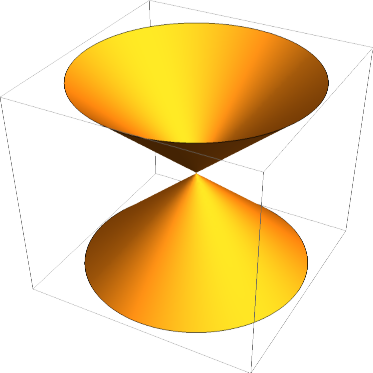
\includegraphics[width=\linewidth]{figures/singular-cone.png}}
\end{Example}

由于仿射簇 $X\subseteq\mathbb{A}^{n}$ 的切空间是 $K^{n}$ 的向量子空间, 自然会预期可用线性代数的工具确定簇的奇异点. 将线性代数工具用于研究切空间和奇异性所需的关键对象是 Jacobian 矩阵. 它只是把有限个多项式的偏导数排成矩阵.

\begin{Definition}{Jacobian 矩阵}\leavevmode\label{def:jacobian-matrix}
给定多项式 $f_{1},\ldots,f_{m}\in K[x_{1},\ldots,x_{n}]$, $f_{1},\ldots,f_{m}$ 的\emph{Jacobian 矩阵}是 $m\times n$ 矩阵
\[
  \operatorname{Jac}_{f_{1},\ldots,f_{m}}=
  \begin{pmatrix}
    \dfrac{\partial f_{1}}{\partial x_{1}} & \cdots & \dfrac{\partial f_{1}}{\partial x_{n}}\\
    \vdots & \ddots & \vdots\\
    \dfrac{\partial f_{m}}{\partial x_{1}} & \cdots & \dfrac{\partial f_{m}}{\partial x_{n}}
  \end{pmatrix}.
\]
\end{Definition}

注意矩阵 $\operatorname{Jac}_{f_{1},\ldots,f_{m}}$ 的元素都属于 $K[x_{1},\ldots,x_{n}]$, 所以可以在任一点 $a\in\mathbb{A}^{n}$ 处取值, 得到 $m\times n$ 矩阵
\[
  \operatorname{Jac}_{f_{1},\ldots,f_{m}}(a)\in K^{mn}.
\]
下一个结果将 $a$ 处的切空间解释为一个 Jacobian 矩阵的核, 由此可用行列式刻画簇的奇异点.

\begin{Proposition}{光滑性的 Jacobian 判据}\leavevmode\label{prop:jacobian-criterion-for-smoothness}
若 $X\subseteq\mathbb{A}^{n}$ 是不可约仿射簇, 且 $\mathcal{I}(X)=\langle f_{1},\ldots,f_{m}\rangle$, 则
\[
  T_{a}X=\ker(\operatorname{Jac}_{f_{1},\ldots,f_{m}}(a)).
\]
因此, $X$ 在 $a\in X$ 处奇异当且仅当
\[
  \operatorname{rk}(\operatorname{Jac}_{f_{1},\ldots,f_{m}}(a))<\operatorname{codim}(X).
\]
\end{Proposition}
\begin{Proof}
注意 $\operatorname{Jac}_{f_{1},\ldots,f_{m}}(a)$ 的各行是函数 $f_{1},\ldots,f_{m}$ 的梯度:
\[
  \operatorname{Jac}_{f_{1},\ldots,f_{m}}(a)=
  \begin{pmatrix}
    \nabla f_{1}(a)\\
    \vdots\\
    \nabla f_{m}(a)
  \end{pmatrix}.
\]
由矩阵乘法的定义, $v\in\ker(\operatorname{Jac}_{f_{1},\ldots,f_{m}}(a))$ 当且仅当对所有 $i=1,\ldots,m$ 都有 $\nabla f_{i}(a)\cdot v=0$. 所以由 Proposition~\ref{prop:gradient-characterization-of-tangent-spaces} 及其证明之后紧接的说明可知
\[
  T_{a}X=\ker(\operatorname{Jac}_{f_{1},\ldots,f_{m}}(a)).
\]
秩--零度定理于是蕴含
\[
  \dim(T_{a}X)=n-\operatorname{rk}(\operatorname{Jac}_{f_{1},\ldots,f_{m}}(a)).
\]
由 Proposition~\ref{prop:tangent-dimension-lower-bound} 可得
\[
  \operatorname{rk}(\operatorname{Jac}_{f_{1},\ldots,f_{m}}(a))\leq\operatorname{codim}(X),
\]
再由光滑点和奇异点的定义, $X$ 在 $a$ 处奇异当且仅当等号不成立.
\end{Proof}

在超曲面的情形, Jacobian 判据特别简单.

\begin{Example}{超曲面的 Jacobian 判据}\leavevmode\label{ex:jacobian-criterion-for-hypersurfaces}
令 $X=\mathcal{V}(f)$, 其中 $f\in K[x_{1},\ldots,x_{n}]$ 不可约, 于是 $\mathcal{I}(X)=\langle f\rangle$. 那么 $\operatorname{codim}(X)=1$, 而 Jacobian 判据表明, $X$ 在 $a$ 处奇异当且仅当 $1\times n$ 矩阵
\[
  \left(\frac{\partial f}{\partial x_{1}}(a)\quad\cdots\quad
    \frac{\partial f}{\partial x_{n}}(a)\right)
\]
的秩为零. 因此 $X$ 在 $a$ 处奇异当且仅当
\[
  \frac{\partial f}{\partial x_{1}}(a)=\cdots=\frac{\partial f}{\partial x_{n}}(a)=0.
\]
\end{Example}

由 Proposition~\ref{prop:jacobian-criterion-for-smoothness}, 簇的奇异点由 Jacobian 矩阵降秩的点刻画. 这一刻画有一个便利的性质: Jacobian 矩阵降秩的点本身就是一组多项式方程的解. 由此得到下面的重要结论.

\begin{Corollary}{奇异点集是闭的}\leavevmode\label{cor:singular-locus-is-closed}
若 $X\subseteq\mathbb{A}^{n}$ 为不可约仿射簇, 且 $\operatorname{Sing}(X)\subseteq X$ 是 $X$ 的奇异点集, 则 $\operatorname{Sing}(X)$ 也是仿射簇.
\end{Corollary}

在给出证明之前, 先回忆: 矩阵 $M$ 的一个 $r\times r$ 子式, 是从 $M$ 删去若干行和列后得到的 $r\times r$ 矩阵的行列式. 线性代数的一个重要结论指出, $\operatorname{rk}(M)<r$ 当且仅当 $M$ 的所有 $r\times r$ 子式都为零.

\begin{Proof}\textbf{of Corollary~\ref{cor:singular-locus-is-closed}.}\quad
选取一组生成元 $\mathcal{I}(X)=\langle f_{1},\ldots,f_{m}\rangle$, 并为简便起见令 $r=\operatorname{codim}(X)$. 由 Proposition~\ref{prop:jacobian-criterion-for-smoothness}, 点 $a\in\mathbb{A}^{n}$ 是 $X$ 的奇异点当且仅当对所有 $i=1,\ldots,m$, $f_{i}(a)=0$, 且
\[
  \operatorname{rk}(\operatorname{Jac}_{f_{1},\ldots,f_{m}}(a))<r.
\]
所以 $\operatorname{Sing}(X)$ 是多项式 $f_{1},\ldots,f_{m}\in K[x_{1},\ldots,x_{n}]$ 和 $\operatorname{Jac}_{f_{1},\ldots,f_{m}}$ 的 $r\times r$ 子式的共同零点集, 其中每个子式都是 $K[x_{1},\ldots,x_{n}]$ 中的多项式.
\end{Proof}

知道 $\operatorname{Sing}(X)$ 是仿射簇后, 就可以用研究仿射簇的所有工具来研究 $\operatorname{Sing}(X)$. 例如可以计算 $\operatorname{Sing}(X)$ 的维数. 下一个例子说明, 不可约超曲面上的\textquotedbl{}几乎所有点\textquotedbl{} (在维数论意义下) 都是光滑点.

\begin{Example}{不可约超曲面的泛光滑性}\leavevmode\label{ex:generic-smoothness-of-irreducible-hypersurfaces}
设 $X=\mathcal{V}(f)\subseteq\mathbb{A}^{n}$, 其中 $f\in K[x_{1},\ldots,x_{n}]$ 不可约. 我们断言 $X$ 至少有一个光滑点. 为论证这一点, 反设 $X$ 的每一点都是奇异点. 由 Jacobian 判据, 这意味着
\[
  \frac{\partial f}{\partial x_{1}},\ldots,\frac{\partial f}{\partial x_{n}}
     \in K[x_{1},\ldots,x_{n}]
\]
都在 $X$ 上取值为零, 所以它们属于消没理想 $\mathcal{I}(X)=\langle f\rangle$. 由于 $f$ 不可约, 它不可能是常数. 不妨假设 $f$ 关于 $x_{1}$ 有正次数. 那么 $\partial f/\partial x_{1}$ 不是零多项式, 且关于 $x_{1}$ 的次数严格小于 $f$ 的次数, 与其属于 $\langle f\rangle$ 矛盾.

因此 $X$ 至少有一个光滑点, 从而 $\operatorname{Sing}(X)\subsetneq X$. 既然 $\operatorname{Sing}(X)$ 和 $X$ 都是仿射簇, 且 $X$ 不可约, 由 Proposition~\ref{prop:dimension-monotonicity} 得 $\dim(\operatorname{Sing}(X))<\dim(X)$. 换句话说, 由于 $\operatorname{Sing}(X)$ 的维数严格小于 $X$ 的维数, 奇异点形成 $X$ 中很特殊的一个点集: $X$ 的几乎所有点都是光滑点. 这一性质常称为\emph{泛光滑性}.
\end{Example}

注意, 泛光滑性对一般的仿射簇也成立. 这由每个仿射簇至少有一个光滑点这一事实推出. 这个一般事实的证明略超出目前讨论的范围.

\BookExerciseHeading
\begin{BookExercises}
  \item\label{ex:smoothness-is-intrinsic} 证明光滑性是仿射簇的内在性质.
  \item\label{ex:singularities-of-nodal-cubic} 考虑仿射簇 $X=\mathcal{V}(y^{2}-x^{3}-x^{2})\subseteq\mathbb{A}^{2}_{\mathbb{C}}$.
  \begin{enumerate}
    \item 画出 $X$ 的实点, 并猜测 $X$ 可能在哪些点处奇异.
    \item 用 Jacobian 判据求出 $X$ 奇异的所有点.
  \end{enumerate}
  \item\label{ex:smooth-affine-double-cover-of-square-free-polynomial} 设 $f\in K[x_{1},\ldots,x_{n}]$ 为无平方因子的多项式, 考虑仿射簇 $X=\mathcal{V}(x_{n+1}^{2}-f)\in\mathbb{A}^{n+1}$.
  \begin{enumerate}
    \item 证明 $X$ 不可约.
    \item 证明 $X$ 光滑.
  \end{enumerate}
  \item\label{ex:complex-unit-sphere-is-smooth} 证明复单位球面 $X=\mathcal{V}(x_{1}^{2}+\cdots+x_{n}^{2}-1)\subseteq\mathbb{A}_{\mathbb{C}}^{n}$ 光滑.
  \item\label{ex:complex-cone-smooth-except-at-origin} 证明复锥面 $\mathcal{V}(x^{2}+y^{2}-z^{2})\subseteq\mathbb{A}^{3}_{\mathbb{C}}$ 在原点处奇异, 在其余各点处光滑.
  \item\label{ex:singular-points-of-whitney-umbrella} 求 Whitney 伞 $\mathcal{V}(x^{2}+y^{2}z)\subseteq\mathbb{A}^{3}$ 的所有奇异点. (Whitney 伞的实点见 Example~\ref{ex:singleton-vanishing-sets} 中的图.)
  \item\label{ex:jacobian-smoothness-of-affine-twisted-cubic} 考虑仿射扭三次曲线 $X=\mathcal{V}(y-x^{2},z-x^{3})\subseteq\mathbb{A}^{3}$. 已知 $X\cong\mathbb{A}^{1}$, 因而 $X$ 光滑. 用 Jacobian 判据给出另一个光滑性证明.
\end{BookExercises}


\chapter{乘积}\label{chap:products}

\noindent\textbf{第 \thechapter{} 章学习目标}
\begin{itemize}
  \item 证明仿射簇的乘积是仿射簇.
  \item 由 $\mathcal{I}(X)$ 和 $\mathcal{I}(Y)$ 确定消没理想 $\mathcal{I}(X\times Y)$.
  \item 描述仿射簇乘积的不可约性, 维数和光滑性与其各因子的关系.
  \item 描述 $R$-模张量积的元素, 并用张量积的规则判定两个元素何时相等.
  \item 在具体例子中, 将 $R$-模和 $R$-代数的张量积与更熟悉的模和代数认同.
  \item 将 $X\times Y$ 的坐标环计算为一个张量积.
\end{itemize}

从已有数学对象构造新对象的一种常见方法是取 Cartesian 积. 例如, 两个加法群的乘积配备逐分量加法后是一个群, 两个拓扑空间的乘积配备乘积拓扑后是一个拓扑空间. 本章试图理解两个仿射簇的 Cartesian 积.

要看出仿射簇的乘积本身也是仿射簇, 需要稍作论证. 做到这点后, 就可以研究乘积的几何性质, 例如不可约性, 维数和光滑性. 本章前两节专门发展这些内容, 最后的结论是: 两个光滑仿射簇 $X$ 和 $Y$ 的乘积是维数为 $\dim(X)+\dim(Y)$ 的光滑仿射簇.

熟悉了仿射簇乘积的几何性质后, 代数与几何的等价性自然引出一个问题: 与几何上的 Cartesian 积相对应的坐标环上的代数运算是什么? 换句话说, $K$-代数 $K[X\times Y]$ 与 $K[X]$ 和 $K[Y]$ 有何关系?

答案是 $K[X\times Y]$ 是 $K[X]$ 与 $K[Y]$ 的张量积. 在 $X=Y=\mathbb{A}^{1}$ 的特殊情形, 这就是说 $K[x,y]$ 是 $K[x]$ 与 $K[y]$ 的张量积. 对许多读者而言, 张量积可能是陌生的, 即便不陌生, 也可能令人望而生畏, 所以我们不假设读者事先了解它. 我们从一个目标出发: 定义一种代数运算, 将 $K[x]$ 和 $K[y]$ 合在一起得到 $K[x,y]$. 围绕这个目标逐步建立定义. 本章最后证明, 对任意仿射簇 $X$ 和 $Y$, 都有 $K[X\times Y]=K[X]\otimes_{K}K[Y]$.

\par\smallskip
{\footnotesize
\noindent\textcopyright{} The Author(s) 2025\par
\noindent E. Clader, D. Ross, \emph{Beginning in Algebraic Geometry}, Undergraduate Texts in Mathematics,
\href{https://doi.org/10.1007/978-3-031-88819-9_9}{\nolinkurl{https://doi.org/10.1007/978-3-031-88819-9_9}}.\par}

\section{仿射簇的乘积}\label{sec:products-of-affine-varieties}

给定仿射簇 $X\subseteq\mathbb{A}^{m}$ 和 $Y\subseteq\mathbb{A}^{n}$, 从集合论角度, 它们的 Cartesian 积 $X\times Y$ 就是下列有序对的集合:
\[
  X\times Y=\{(a,b)\mid a\in X,\ b\in Y\}\subseteq\mathbb{A}^{m}\times\mathbb{A}^{n}.
\]
\BookPairedNote
  {另一方面, $\mathbb{A}^{m}\times\mathbb{A}^{n}$ 可以与 $\mathbb{A}^{m+n}$ 典范地认同, 所以可将 $X\times Y$ 直接看成某个仿射空间的子集: $X\times Y\subseteq\mathbb{A}^{m+n}$.}
  {下面将对 $\mathbb{A}^{m}$ 和 $\mathbb{A}^{n}$ 使用不同的变量, 以免混淆这两个仿射空间.}
第一个目标是证明, 在 $\mathbb{A}^{m+n}$ 中, 集合 $X\times Y$ 本身就是仿射簇.

\begin{Proposition}{仿射簇的乘积是仿射簇}\leavevmode\label{prop:product-of-affine-varieties-is-affine}\strut\par\nopagebreak[4]\noindent
若 $X=\mathcal{V}(f_{1},\ldots,f_{r})\subseteq\mathbb{A}^{m}$ 且 $Y=\mathcal{V}(g_{1},\ldots,g_{s})\subseteq\mathbb{A}^{n}$, 其中 $f_{1},\ldots,f_{r}\in K[x_{1},\ldots,x_{m}]$ 且 $g_{1},\ldots,g_{s}\in K[y_{1},\ldots,y_{n}]$, 则
\[
  X\times Y=\mathcal{V}(f_{1},\ldots,f_{r},g_{1},\ldots,g_{s})\subseteq\mathbb{A}^{m+n},
\]
其中把多项式 $f_{1},\ldots,f_{r}$ 和 $g_{1},\ldots,g_{s}$ 看成较大的多项式环 $K[x_{1},\ldots,x_{m},y_{1},\ldots,y_{n}]$ 的元素.
\end{Proposition}
\begin{Proof}
\BookPairedNoteLeft
  {按定义, $\mathbb{A}^{m+n}$ 中的点 $(a,b)=(a_{1},\ldots,a_{m},b_{1},\ldots,b_{n})$ 属于 $X\times Y$, 当且仅当 $a\in X$ 且 $b\in Y$. 由 $X$ 和 $Y$ 的定义, 这当且仅当}
  {虽然 Proposition~\ref{prop:product-of-affine-varieties-is-affine} 针对两个仿射簇的乘积陈述, 但它自然可推广到有限 Cartesian 积 (Exercise~\ref{ex:finite-product-of-affine-varieties}).}
\[
  f_{1}(a)=\cdots=f_{r}(a)=0
  \qquad\text{且}\qquad g_{1}(b)=\cdots=g_{s}(b)=0.
\]
若把 $f_{1},\ldots,f_{r}$ 看作 $K[x_{1},\ldots,x_{m},y_{1},\ldots,y_{n}]$ 中恰好只涉及前 $m$ 个变量的元素, 则 $f_{i}(a,b)=f_{i}(a)$. 类似地, $g_{j}(a,b)=g_{j}(b)$. 因此 $(a,b)\in X\times Y$ 当且仅当
\[
  f_{1}(a,b)=\cdots=f_{r}(a,b)=g_{1}(a,b)=\cdots=g_{s}(a,b)=0,
\]
这恰好就是说 $X\times Y=\mathcal{V}(f_{1},\ldots,f_{r},g_{1},\ldots,g_{s})$.
\end{Proof}

\begin{Example}{$\mathbb{A}^{3}$ 中平行的抛物线}\leavevmode\label{ex:product-parallel-parabolas}
令 $X=\mathcal{V}(y-x^{2})\subseteq\mathbb{A}^{2}$ 和 $Y=\mathcal{V}(z^{2}-1)\subseteq\mathbb{A}^{1}$, 于是 $X$ 是 $\mathbb{A}^{2}$ 中的一条抛物线, 而 $Y$ 是 $\mathbb{A}^{1}$ 中的两个点 $\{\pm1\}$. 那么
\[
  X\times Y=\mathcal{V}(y-x^{2},z^{2}-1)\subseteq\mathbb{A}^{3},
\]
可把它想象成两条平行的抛物线, 分别位于高度为 $\pm1$ 且平行于 $xy$ 平面的两个平面内.
\end{Example}

\begin{Example}{圆柱面}\leavevmode\label{ex:product-circle-line-cylinder}
令 $X=\mathcal{V}(x^{2}+y^{2}-1)\subseteq\mathbb{A}^{2}$ 且 $Y=\mathbb{A}^{1}$. 那么
\[
  X\times Y=\mathcal{V}(x^{2}+y^{2}-1)\subseteq\mathbb{A}^{3},
\]
在实数域上, 它就是\hyperref[fig:circle-times-line-cylinder]{下图}中的圆柱面.
\par\smallskip
{\centering\phantomsection\label{fig:circle-times-line-cylinder}%
  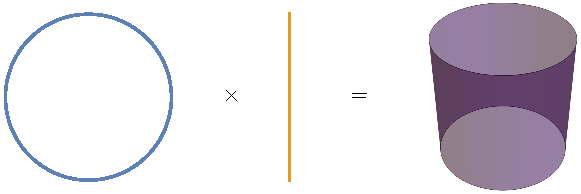
\includegraphics[width=.85\linewidth]{figures/circle-times-line-cylinder.pdf}\par}
\end{Example}

知道仿射簇的乘积本身也是仿射簇, 是研究乘积的重要第一步. 不过, 要研究坐标环, 维数和切空间, 还需要了解它们的消没理想.

\begin{Proposition}{乘积的消没理想}\leavevmode\label{prop:vanishing-ideal-of-product}
设 $X\subseteq\mathbb{A}^{m}$ 和 $Y\subseteq\mathbb{A}^{n}$ 为仿射簇. 则
\[
  \mathcal{I}(X\times Y)=\langle\mathcal{I}(X)\rangle+\langle\mathcal{I}(Y)\rangle,
\]
其中把 $\mathcal{I}(X)\subseteq K[x_{1},\ldots,x_{m}]$ 和 $\mathcal{I}(Y)\subseteq K[y_{1},\ldots,y_{n}]$ 看作较大多项式环 $K[x_{1},\ldots,x_{m},\allowbreak y_{1},\ldots,y_{n}]$ 的子集.
\end{Proposition}

\BookPairedNote
  {注意, 把 $\mathcal{I}(X)$ 和 $\mathcal{I}(Y)$ 看成 $K[x_{1},\ldots,x_{m},y_{1},\ldots,y_{n}]$ 的子集时, 它们不是理想. 所以先取它们各自生成的理想, 再取理想的和.}
  {回忆, 理想的和定义为 $I+J=\{a+b\mid a\in I,\ b\in J\}$.}
给定生成元 $\mathcal{I}(X)=\langle f_{1},\ldots,f_{k}\rangle$ 和 $\mathcal{I}(Y)=\langle g_{1},\ldots,g_{\ell}\rangle$, Proposition~\ref{prop:vanishing-ideal-of-product} 蕴含 (Exercise~\ref{ex:product-ideal-from-generators})
\[
  \mathcal{I}(X\times Y)=\langle f_{1},\ldots,f_{k},g_{1},\ldots,g_{\ell}\rangle
    \subseteq K[x_{1},\ldots,x_{m},y_{1},\ldots,y_{n}].
\]

\begin{Proof}\textbf{of Proposition~\ref{prop:vanishing-ideal-of-product}.}\quad
注意 $\langle\mathcal{I}(X)\rangle$ 的一般元素形如
\[
  h_{1}f_{1}+\cdots+h_{k}f_{k},
\]
其中 $h_{1},\ldots,h_{k}\in K[x_{1},\ldots,x_{m},y_{1},\ldots,y_{n}]$, 且 $f_{1},\ldots,f_{k}\in\mathcal{I}(X)$. 将任意这样的多项式在 $(a,b)\in X\times Y$ 处取值, 得
\[
  h_{1}(a,b)f_{1}(a)+\cdots+h_{k}(a,b)f_{k}(a)=0,
\]
因为对所有 $a\in X$, 有 $f_{1}(a)=\cdots=f_{k}(a)=0$. 类似的论证表明, $\langle\mathcal{I}(Y)\rangle$ 中的任意多项式在 $X\times Y$ 的每一点处都取值为零. 所以 $\langle\mathcal{I}(X)\rangle+\langle\mathcal{I}(Y)\rangle$ 的每个多项式都在 $X\times Y$ 上取值为零, 这表明
\[
  \langle\mathcal{I}(X)\rangle+\langle\mathcal{I}(Y)\rangle\subseteq\mathcal{I}(X\times Y).
\]

为证明反向包含, 设 $h\in\mathcal{I}(X\times Y)$. 总能找到形如
\begin{equation}\label{eq:polynomial-sum-of-separated-products}
  h=f_{1}g_{1}+\cdots+f_{k}g_{k}
\end{equation}
的表达式, 其中 $f_{1},\ldots,f_{k}\in K[x_{1},\ldots,x_{m}]$, 且 $g_{1},\ldots,g_{k}\in K[y_{1},\ldots,y_{n}]$ (例如, 将 $h$ 写成单项式之和, 再在每个单项式中把 $x$ 变量和 $y$ 变量分开). 对任意形如 \eqref{eq:polynomial-sum-of-separated-products} 的表达式, 重排后可设 $g_{1},\ldots,g_{j}\notin\mathcal{I}(Y)$, 而 $g_{j+1},\ldots,g_{k}\in\mathcal{I}(Y)$. 固定一个使 $j$ 最小的这种表达式. 对这个 $j$ 最小的表达式, 我们断言 $f_{1},\ldots,f_{j}\in\mathcal{I}(X)$, 由此得到
\[
  \begin{aligned}
    h&=f_{1}g_{1}+\cdots+f_{j}g_{j}+f_{j+1}g_{j+1}+\cdots+f_{k}g_{k}\\
     &\in\langle\mathcal{I}(X)\rangle+\langle\mathcal{I}(Y)\rangle,
  \end{aligned}
\]
从而结论得证.

为证明断言, 反设 $f_{1},\ldots,f_{j}$ 中有一个不属于 $\mathcal{I}(X)$. 不妨设对某个 $a\in X$ 有 $f_{1}(a)\neq0$. 定义
\[
  g=h(a,y)=f_{1}(a)g_{1}+f_{2}(a)g_{2}+\cdots+f_{k}(a)g_{k}
    \in K[y_{1},\ldots,y_{n}].
\]
由于 $h$ 在 $X\times Y$ 上取值为零, 可知 $g\in\mathcal{I}(Y)$. 解出 $g_{1}$ 得
\[
  g_{1}=f_{1}(a)^{-1}\bigl(g-f_{2}(a)g_{2}-\cdots-f_{k}(a)g_{k}\bigr).
\]
将该表达式代入 \eqref{eq:polynomial-sum-of-separated-products} 中的 $g_{1}$, 得到 $h$ 的一个如下形式的表达式:
\[
  \begin{aligned}
    h={}&\bigl(f_{2}-f_{1}(a)^{-1}f_{2}(a)f_{1}\bigr)g_{2}+\cdots\\
        &{}+\bigl(f_{k}-f_{1}(a)^{-1}f_{k}(a)f_{1}\bigr)g_{k}+f_{1}(a)^{-1}f_{1}g.
  \end{aligned}
\]
在这个新表达式中, $g_{2},\ldots,g_{j}\notin\mathcal{I}(Y)$, 而 $g_{j+1},\ldots,g_{k},g\in\mathcal{I}(Y)$, 与 $j$ 的最小性矛盾, 证明完毕.
\end{Proof}

Proposition~\ref{prop:vanishing-ideal-of-product} 使我们可以计算乘积的坐标环:
\[
  K[X\times Y]=\frac{K[x_{1},\ldots,x_{m},y_{1},\ldots,y_{n}]}
    {\langle\mathcal{I}(X)\rangle+\langle\mathcal{I}(Y)\rangle}.
\]
不过, 这个描述有一点令人不满意: 它要求从外在角度把 $X$ 和 $Y$ 都看作仿射空间的子集, 而不是只看作仿射簇的同构类. 因此自然会问: 能否仅用两个坐标环 $K[X]$ 和 $K[Y]$ 从内在角度计算坐标环 $K[X\times Y]$?

这个问题最理想的答案是给出一种代数运算 $\star$, 使得对所有仿射簇 $X$ 和 $Y$ 都有
\[
  K[X]\star K[Y]=K[X\times Y].
\]
无论 $\star$ 是什么, 它必有一个特例
\[
  K[x]\star K[y]=K[x,y],
\]
这是取 $X=Y=\mathbb{A}^{1}$, 从而 $X\times Y=\mathbb{A}^{2}$ 得到的.

这时读者或许会想, 目前知道哪些方法, 可以把两个 $K$-代数 $A$ 和 $B$ 合成一个新 $K$-代数 $A\star B$? 首先想到的运算可能是直和 $A\oplus B$. 可惜这并不是所需的运算. $A\oplus B$ 上的自然环结构是逐分量的:
\[
  \begin{aligned}
    (a_{1},b_{1})+(a_{2},b_{2})&=(a_{1}+a_{2},b_{1}+b_{2}),\\
    (a_{1},b_{1})\cdot(a_{2},b_{2})&=(a_{1}a_{2},b_{1}b_{2}),
  \end{aligned}
\]
读者可验证 (Exercise~\ref{ex:direct-sum-of-nonzero-rings-is-not-domain}), 这决不会产生整环. 所以 $K[x,y]$ 不可能与 $K[x]\oplus K[y]$ 相同.

我们很快会看到, 运算 $\star$ 的正确选择是 $K$-代数的张量积. 第~\ref{sec:tensor-products-of-modules} 和~\ref{sec:tensor-products-and-bilinearity}~节发展张量积的代数基础, 最后在第~\ref{sec:coordinate-rings-of-products}~节证明, 张量积确实给出了仿射簇乘积的坐标环. 不过, 在深入张量积之前, 先在第~\ref{sec:geometric-properties-of-products}~节研究乘积的关键几何性质, 回答关于不可约性, 维数和光滑性的自然问题.

\BookExerciseHeading
\begin{BookExercises}
  \item\label{ex:draw-product-finite-set-and-line} 令 $X=\mathcal{V}(x^{2}-1)\subseteq\mathbb{A}^{1}$ 和 $Y=\mathcal{V}(y-z)\subseteq\mathbb{A}^{2}$. 画出 $X\times Y\subseteq\mathbb{A}^{3}$ 在 $\mathbb{R}$ 上的图形.
  \item\label{ex:recognize-product-of-finite-sets} 画出仿射簇
  \[
    Z=\mathcal{V}(x+z^{2}-z,x)\subseteq\mathbb{A}^{3}=\mathbb{A}^{2}\times\mathbb{A}^{1}
  \]
  在 $\mathbb{R}$ 上的图形. 是否存在仿射簇 $X\subseteq\mathbb{A}^{2}$ 和 $Y\subseteq\mathbb{A}^{1}$ 使 $Z=X\times Y$? 若是, 给出这样的 $X$ 和 $Y$ 的一个例子. 若否, 如何看出?
  \item\label{ex:coordinate-planes-as-product-or-not} 画出仿射簇
  \[
    Z=\mathcal{V}(xyz)\subseteq\mathbb{A}^{3}=\mathbb{A}^{2}\times\mathbb{A}^{1}
  \]
  在 $\mathbb{R}$ 上的图形. 是否存在仿射簇 $X\subseteq\mathbb{A}^{2}$ 和 $Y\subseteq\mathbb{A}^{1}$ 使 $Z=X\times Y$? 若是, 给出这样的 $X$ 和 $Y$ 的一个例子. 若否, 如何看出?
  \item\label{ex:finite-product-of-affine-varieties} 将 Proposition~\ref{prop:product-of-affine-varieties-is-affine} 推广到有限个仿射簇的乘积, 并证明.
  \item\label{ex:product-ideal-from-generators} 设 $X\subseteq\mathbb{A}^{m}$ 和 $Y\subseteq\mathbb{A}^{n}$ 为仿射簇. 若 $\mathcal{I}(X)=\langle f_{1},\ldots,f_{k}\rangle$ 且 $\mathcal{I}(Y)=\langle g_{1},\ldots,g_{\ell}\rangle$, 证明
  \[
    \mathcal{I}(X\times Y)=\langle f_{1},\ldots,f_{k},g_{1},\ldots,g_{\ell}\rangle
      \subseteq K[x_{1},\ldots,x_{m},y_{1},\ldots,y_{n}].
  \]
  \item\label{ex:products-of-affine-varieties-are-intrinsic} 设 $X,X',Y,Y'$ 为仿射簇, 且 $X\cong X'$ 和 $Y\cong Y'$. 证明
  \[
    X\times Y\cong X'\times Y'.
  \]
  换句话说, 仿射簇的乘积是内在的.
  \item\label{ex:direct-sum-of-nonzero-rings-is-not-domain} 证明若 $A$ 和 $B$ 是非零环, 则配备逐分量加法和乘法的环 $A\oplus B$ 不是整环.
\end{BookExercises}

\section{乘积的性质}\label{sec:geometric-properties-of-products}

先用下面这个关于不可约性的核心结论, 开始研究乘积的几何性质. 它对于研究乘积的维数和光滑性都有用.

\begin{Proposition}{不可约簇的乘积不可约}\leavevmode\label{prop:product-of-irreducible-varieties-is-irreducible}
若 $X$ 和 $Y$ 为不可约仿射簇, 则 $X\times Y$ 不可约.
\end{Proposition}

着手证明之前, 先看几个具体例子, 了解不可约性与乘积之间的关系.

\begin{Example}{不可约的乘积}\leavevmode\label{ex:irreducible-parabola-product}
若 $X=\mathcal{V}(y-x^{2})\subseteq\mathbb{A}^{2}$ 且 $Y=\mathcal{V}(z-1)\subseteq\mathbb{A}^{1}$, 则 $X$ 和 $Y$ 都不可约, 而乘积
\[
  X\times Y=\mathcal{V}(y-x^{2},z-1)\subseteq\mathbb{A}^{3}
\]
是 $\mathbb{A}^{3}$ 中的一条抛物线. $X\times Y$ 的不可约性可以由同构 $X\times Y\cong X$ 看出, 这个同构就是垂直投影 $\mathbb{A}^{3}\to\mathbb{A}^{2}$ 的限制.
\end{Example}

\begin{Example}{可约的乘积}\leavevmode\label{ex:reducible-cross-times-line}
令 $X=\mathcal{V}(xy)\subseteq\mathbb{A}^{2}$ 且 $Y=\mathbb{A}^{1}$. 那么 $X=\mathcal{V}(x)\cup\mathcal{V}(y)$ 是可约的, 乘积也可约:
\[
  X\times Y=\mathcal{V}(x)\cup\mathcal{V}(y)\subseteq\mathbb{A}^{3},
\]
如\hyperref[fig:axes-times-line-intersecting-planes]{下图}所示.
\par\smallskip
{\centering\phantomsection\label{fig:axes-times-line-intersecting-planes}%
  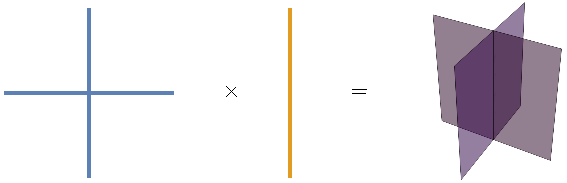
\includegraphics[width=.85\linewidth]{figures/axes-times-line-intersecting-planes.pdf}\par}

尽管 $Y$ 是整个仿射空间, 因而这个例子大为简化, 它仍体现了 Proposition~\ref{prop:product-of-irreducible-varieties-is-irreducible} 的证明要点: 若 $Y$ 不可约, 则把 $X\times Y$ 分解成两个仿射簇的并, 只能来自把 $X$ 作类似的分解.
\end{Example}

\begin{Proof}\textbf{of Proposition~\ref{prop:product-of-irreducible-varieties-is-irreducible}.}\quad
设 $X\subseteq\mathbb{A}^{m}$ 和 $Y\subseteq\mathbb{A}^{n}$ 为不可约仿射簇. 为证明 $X\times Y$ 不可约, 要说明对仿射簇 $Z_{1},Z_{2}\subseteq X\times Y\subseteq\mathbb{A}^{m+n}$, 只有当 $Z_{1}=X\times Y$ 或 $Z_{2}=X\times Y$ 时, 才能有
\begin{equation}\label{eq:product-as-union-of-two-varieties}
  X\times Y=Z_{1}\cup Z_{2}.
\end{equation}

设 \eqref{eq:product-as-union-of-two-varieties} 成立. 对每一点 $a\in X$, 考虑集合
\[
  \{a\}\times Y\subseteq X\times Y.
\]
例如, 若 $X\times Y$ 是 Example~\ref{ex:product-circle-line-cylinder} 的圆柱面或 Example~\ref{ex:reducible-cross-times-line} 的相交平面, 那么集合 $\{a\}\times Y$ 就是乘积中的那些垂直直线. 每个集合 $\{a\}\times Y$ 都是仿射簇 (因为 $\{a\}$ 和 $Y$ 都是仿射簇), 且它们都同构于 $Y$. 因此 $Y$ 不可约意味着对所有 $a\in X$, $\{a\}\times Y$ 不可约. 将 \eqref{eq:product-as-union-of-two-varieties} 两边与 $\{a\}\times Y$ 相交, 得
\[
  \{a\}\times Y
    =\bigl((\{a\}\times Y)\cap Z_{1}\bigr)\cup
     \bigl((\{a\}\times Y)\cup Z_{2}\bigr).
\]
由于 $\{a\}\times Y$ 不可约, 必有
\[
  (\{a\}\times Y)\cap Z_{1}=\{a\}\times Y
  \quad\text{或}\quad
  (\{a\}\times Y)\cap Z_{2}=\{a\}\times Y.
\]
换句话说, 对任意 $a\in X$, 或者 $\{a\}\times Y\subseteq Z_{1}$, 或者 $\{a\}\times Y\subseteq Z_{2}$. 因此, 定义两个集合
\[
  X_{1}=\{a\in X\mid\{a\}\times Y\subseteq Z_{1}\}
  \quad\text{且}\quad
  X_{2}=\{a\in X\mid\{a\}\times Y\subseteq Z_{2}\},
\]
就有
\begin{equation}\label{eq:base-as-union-of-full-fiber-loci}
  X_{1}\cup X_{2}=X.
\end{equation}
到此只知道 $X_{1}$ 和 $X_{2}$ 是 $X$ 的子集, 但它们本身实际上也是仿射簇. 为看出这一点, 回忆 $Z_{1}$ 是仿射簇, 因此
\[
  Z_{1}=\mathcal{V}(f_{1},\ldots,f_{r})
\]
其中 $f_{1},\ldots,f_{r}\in K[x_{1},\ldots,x_{m},y_{1},\ldots,y_{n}]$ 为某些多项式. 对任意 $b\in Y$, 考虑仿射簇
\[
  (X_{1})_{b}=\mathcal{V}\bigl(f_{1}(x,b),\ldots,f_{r}(x,b)\bigr)\subseteq\mathbb{A}^{m},
\]
并注意
\[
  (X_{1})_{b}=\{a\in\mathbb{A}^{m}\mid(a,b)\in Z_{1}\}.
\]
进一步有
\[
  X_{1}=\{a\in X\mid(a,b)\in Z_{1}\text{ 对所有 }b\in Y\}
    =X\cap\bigcap_{b\in Y}(X_{1})_{b},
\]
所以 $X_{1}$ 是仿射簇的交, 因而是仿射簇. 同样的论证适用于 $X_{2}$.

回顾等式 \eqref{eq:base-as-union-of-full-fiber-loci}, 已将 $X$ 表成两个仿射簇的并. 由于 $X$ 不可约, 只有当 $X_{1}=X$ 或 $X_{2}=X$ 时才可能. 若 $X_{1}=X$, 则对所有 $a\in X$, 都有 $\{a\}\times Y\subseteq Z_{1}$, 换句话说 $X\times Y\subseteq Z_{1}$, 从而 $X\times Y=Z_{1}$. 同理, 若 $X_{2}=X$, 则对所有 $a\in X$ 都有 $\{a\}\times Y\subseteq Z_{2}$, 换句话说 $X\times Y\subseteq Z_{2}$, 从而 $X\times Y=Z_{2}$. 已证明 $X\times Y=Z_{1}$ 或 $X\times Y=Z_{2}$, 这就完成了 $X\times Y$ 不可约的证明.
\end{Proof}

Proposition~\ref{prop:product-of-irreducible-varieties-is-irreducible} 给出乘积的不可约分解的如下描述. 建议读者在 Exercise~\ref{ex:prove-irreducible-components-of-product} 中证明它.

\begin{Corollary}{乘积的不可约分解}\leavevmode\label{cor:irreducible-components-of-product}
若仿射簇 $X$ 和 $Y$ 的不可约分支分别为 $X_{1},\ldots,X_{k}$ 和 $Y_{1},\ldots,Y_{\ell}$, 那么 $X\times Y$ 的不可约分支是对所有 $i=1,\ldots,k$ 和 $j=1,\ldots,\ell$ 得到的仿射簇 $X_{i}\times Y_{j}$.
\end{Corollary}

现在转向维数. 无论是类比向量空间的维数, 还是直观地把维数看作一个点可以移动的独立方向数, 都会自然预期 $\dim(X\times Y)=\dim(X)+\dim(Y)$. 下一个结果说明这个预期确实成立.

\begin{Proposition}{维数对乘积可加}\leavevmode\label{prop:dimension-additive-on-products}
若 $X$ 和 $Y$ 是非空仿射簇, 则
\[
  \dim(X\times Y)=\dim(X)+\dim(Y).
\]
\end{Proposition}
\begin{Proof}
对 $\dim(X)+\dim(Y)$ 归纳.

(归纳起点) 若 $\dim(X)+\dim(Y)=0$, 则 $\dim(X)=\dim(Y)=0$, 所以 $X$ 和 $Y$ 各是有限点集. 由于有限集的 Cartesian 积是有限集, $X\times Y$ 是有限集, 从而 $\dim(X\times Y)=0=\dim(X)+\dim(Y)$.

(归纳步骤) 令 $d>0$, 并假设只要各因子的维数之和小于 $d$, 维数对乘积就可加. 设 $X\subseteq\mathbb{A}^{m}$ 和 $Y\subseteq\mathbb{A}^{n}$ 是非空仿射簇, 且 $\dim(X)+\dim(Y)=d$. 要证明 $\dim(X\times Y)=\dim(X)+\dim(Y)$.

将 $X$ 和 $Y$ 分解为不可约分支后, Corollary~\ref{prop:dimension-additive-on-products} 蕴含 $X\times Y$ 的维数是 $X_{i}\times Y_{j}$ 的维数的最大值, 其中 $X_{i}$ 和 $Y_{j}$ 分别是 $X$ 和 $Y$ 的不可约分支. 因而, 若归纳步骤的结论对 $X$ 和 $Y$ 的不可约分支成立, 就对 $X$ 和 $Y$ 成立. 所以只须对不可约仿射簇证明归纳步骤, 下面假设 $X$ 和 $Y$ 不可约, 从而 $X\times Y$ 不可约.

由于 $\dim(X)+\dim(Y)>0$, 不妨设 $\dim(X)>0$. 因而 $X$ 有不止一个点, 可找到多项式 $f\in K[x_{1},\ldots,x_{m}]$ 使 $\varnothing\subsetneq\mathcal{V}(f)\cap X\subsetneq X$. 也把该多项式看成 $K[x_{1},\ldots,x_{m},y_{1},\ldots,y_{n}]$ 的元素, 有
\[
  \mathcal{V}(f)\cap(X\times Y)=(\mathcal{V}(f)\cap X)\times Y.
\]
对上述等式的两边应用维数论基本定理, 就得到所需结论:
\[
  \begin{aligned}
    \dim(X\times Y)&=\dim(\mathcal{V}(f)\cap(X\times Y))+1\\
      &=\dim((\mathcal{V}(f)\cap X)\times Y)+1\\
      &=(\dim(X)-1)+\dim(Y)+1=\dim(X)+\dim(Y),
  \end{aligned}
\]
其中第三个等号使用了归纳假设.
\end{Proof}

现在可以讨论本节最后一个话题: 仿射簇乘积的光滑性. 由于光滑性由切空间定义, 而切空间由线性化定义, 因此下面关于乘积的线性化和切空间的结论是证明光滑仿射簇的乘积仍光滑的关键步骤. (这个陈述用到向量空间的直和 $V\oplus W$. 提醒读者, 这是由有序对 $(v,w)$ 组成的向量空间, 其中 $v\in V$, $w\in W$, 维数为 $\dim(V)+\dim(W)$.)

\begin{Proposition}{乘积的切空间}\leavevmode\label{prop:tangent-space-of-product}
若 $X\subseteq\mathbb{A}^{m}$ 和 $Y\subseteq\mathbb{A}^{n}$ 是仿射簇, $a\in X$, $b\in Y$, 则
\[
  L_{(a,b)}(X\times Y)=L_{a}X\times L_{b}Y
  \quad\text{且}\quad
  T_{(a,b)}(X\times Y)=T_{a}X\oplus T_{b}Y.
\]
\end{Proposition}
\begin{Proof}
设 $\mathcal{I}(X)=\langle f_{1},\ldots,f_{k}\rangle$ 和 $\mathcal{I}(Y)=\langle g_{1},\ldots,g_{\ell}\rangle$. 由 Proposition~\ref{prop:vanishing-ideal-of-product} 及紧随其后的讨论, 有
\[
  \mathcal{I}(X\times Y)=\langle f_{1},\ldots,f_{k},g_{1},\ldots,g_{\ell}\rangle.
\]
如第~\ref{sec:linearizations-and-tangent-spaces}~节所见, 可将线性化算作
\[
  \begin{aligned}
    L_{a}X&=\mathcal{V}(L_{a}f_{1},\ldots,L_{a}f_{k}),\\
    L_{b}Y&=\mathcal{V}(L_{b}g_{1},\ldots,L_{b}g_{\ell}),\\
    L_{(a,b)}(X\times Y)&=\mathcal{V}(L_{a}f_{1},\ldots,L_{a}f_{k},L_{b}g_{1},\ldots,L_{b}g_{\ell}),
  \end{aligned}
\]
这里用到 $L_{(a,b)}f_{i}=L_{a}f_{i}$, 因为 $f_{i}\in K[x_{1},\ldots,x_{m}]$, 对 $g_{j}$ 也类似. 因此由 Proposition~\ref{prop:product-of-affine-varieties-is-affine} 得 $L_{(a,b)}(X\times Y)=L_{a}X\times L_{b}Y$.

为证明关于切空间的陈述, 回忆第~\ref{sec:linearizations-and-tangent-spaces}~节中
\[
  T_{a}X=\{\overrightarrow{aa'}\mid a'\in L_{a}X\}\subseteq K^{m}
  \quad\text{且}\quad
  T_{b}Y=\{\overrightarrow{bb'}\mid b'\in L_{b}Y\}\subseteq K^{n}.
\]
因此向量空间 $T_{a}X\oplus T_{b}Y\subseteq K^{m}\oplus K^{n}$ 由形如
\[
  \bigl(\overrightarrow{aa'},\overrightarrow{bb'}\bigr)
\]
的向量组成, 其中 $a'\in L_{a}X$, $b'\in L_{b}Y$. 在认同 $K^{m}\oplus K^{n}=K^{m+n}$ 后, 有
\[
  \bigl(\overrightarrow{aa'},\overrightarrow{bb'}\bigr)
    =\overrightarrow{(a,b)(a',b')}.
\]
因而
\[
  T_{a}X\oplus T_{b}Y
    =\{\overrightarrow{(a,b)(a',b')}\mid(a',b')\in L_{a}X\times L_{b}Y\}
    =T_{(a,b)}(X\times Y),
\]
其中最后一个等号用到 $L_{a}X\times L_{b}Y=L_{(a,b)}(X\times Y)$.
\end{Proof}

现在很快可推出光滑仿射簇的乘积是光滑的.

\begin{Corollary}{光滑簇的乘积光滑}\leavevmode\label{cor:product-of-smooth-varieties-is-smooth}
若 $X$ 和 $Y$ 是光滑仿射簇, 则 $X\times Y$ 也是光滑仿射簇.
\end{Corollary}
\begin{Proof}
设 $X$ 和 $Y$ 是光滑的 (不可约) 仿射簇. 给定任意 $(a,b)\in X\times Y$, 有
\[
  \begin{aligned}
    \dim(X\times Y)&=\dim(X)+\dim(Y)\\
      &=\dim(T_{a}X)+\dim(T_{b}Y)\\
      &=\dim(T_{a}X\oplus T_{b}Y)\\
      &=\dim(T_{(a,b)}(X\times Y)),
  \end{aligned}
\]
其中第一个等号是 Proposition~\ref{prop:dimension-additive-on-products}, 第二个用到 $X$ 和 $Y$ 都光滑的假设, 第三个来自向量空间的维数对直和可加, 第四个是 Proposition~\ref{prop:tangent-space-of-product} 的第二个陈述. 由光滑性的定义可知 $X\times Y$ 光滑.
\end{Proof}

熟悉了仿射簇的乘积及其性质后, 本章的余下部分用于发展乘积坐标环的一种内在构造. 如上一节末尾所说, 所需的关键构造是张量积. 接下来两节发展张量积的代数基础, 着眼于多项式环的张量积. 在本章最后一节, 将用这些结果论证乘积的坐标环确实是各因子的坐标环的张量积.

\BookExerciseHeading
\begin{BookExercises}
  \item\label{ex:converse-of-product-irreducibility} Proposition~\ref{prop:product-of-irreducible-varieties-is-irreducible} 的逆命题是否成立? 给出证明或反例.
  \item\label{ex:irreducible-decomposition-of-axes-times-two-points} 令 $X=\mathcal{V}(xy)\subseteq\mathbb{A}^{2}$, $Y=\mathcal{V}(z^{2}-1)\subseteq\mathbb{A}^{1}$. 描述 $X\times Y$ 并计算它的不可约分解.
  \item\label{ex:prove-irreducible-components-of-product} 证明 Corollary~\ref{cor:irreducible-components-of-product}.
  \item\label{ex:converse-of-product-smoothness} Corollary~\ref{cor:product-of-smooth-varieties-is-smooth} 的逆命题是否成立? 更具体地说, 若 $X$ 和 $Y$ 不可约且 $X\times Y$ 光滑, 这是否蕴含 $X$ 和 $Y$ 都光滑? 给出证明或反例.
  \item\label{ex:generalize-product-property-to-many-factors} 从本节的五个结果中选一个, 陈述它对有限个仿射簇乘积的推广. 用归纳论证从两个因子的情形推出一般陈述.
\end{BookExercises}

\par\medskip
{\footnotesize
\noindent\textbf{开放获取.} 本章按照
\href{http://creativecommons.org/licenses/by-nc/4.0/}{Creative Commons Attribution-NonCommercial 4.0 International License}
的条款授权. 该许可允许以任何媒介或格式进行非商业性使用, 分享, 改编, 分发和复制, 但须对原作者和来源作适当署名, 提供 Creative Commons 许可的链接, 并说明是否作了修改.

\noindent
\begin{minipage}[t]{.17\linewidth}
  \vspace{0pt}
\includegraphics[width=.9\linewidth]{figures/source-cc-by-nc.png}
\end{minipage}\hfill
\begin{minipage}[t]{.81\linewidth}
  \vspace{0pt}本章的图片或其他第三方材料均纳入本章的 Creative Commons 许可, 除非材料的署名行另有注明. 如果材料未纳入本章的 Creative Commons 许可, 且您拟进行的使用未获法律规定的许可或超出允许使用的范围, 则须直接向著作权持有人取得许可.
\end{minipage}\par}

\section{模与代数的张量积}\label{sec:tensor-products-of-modules}

本节的目标是定义张量积 $M\otimes_{R}N$, 即从 $R$-模 $M$ 和 $N$ 构造的一个 $R$-模. 此外, 如果 $M$ 和 $N$ 恰好是 $R$-代数, 张量积还将继承 $R$-代数的结构. 典型的情形是 $M=R[x]$ 且 $N=R[y]$, 这时将有
\[
  R[x]\otimes_{R}R[y]=R[x,y].
\]
为理解怎样把这个例子推广到一般的模, 我们着眼于 $R[x,y]$ 的一条关键性质. 这条性质已经在 Proposition~\ref{prop:vanishing-ideal-of-product} 的证明中遇到: 每个多项式 $h\in R[x,y]$ 都可以 (不唯一地) 表成和
\[
  h=f_{1}g_{1}+f_{2}g_{2}+\cdots+f_{k}g_{k},
\]
其中 $f_{1},\ldots,f_{k}\in R[x]$, $g_{1},\ldots,g_{k}\in R[y]$. 例如, $3x^{2}y+2x+4xy^{2}$ 可以写成三项之和
\[
  (3x^{2})\cdot y+(2x)\cdot1+(4x)\cdot y^{2}.
\]
\BookPairedNote
  {现在设 $M$ 和 $N$ 为任意 $R$-模. 若 $f_{i}\in M$ 且 $g_{i}\in N$, 可以把\textquotedbl{}乘积\textquotedbl{} $f_{i}g_{i}$ 在形式上理解为 $M\times N$ 的一个元素.}
  {回忆, 在 (带单位元的) 环 $R$ 中, 数 $3$ 表示 $1+1+1$.}
因此, 定义 $M\otimes_{R}N$ 的第一步是构造一个 $R$-模, 使这样的乘积在其中可以相加. 出发点是形式线性组合的概念.

\begin{Definition}{形式线性组合}\leavevmode\label{def:formal-linear-combination}
设 $S$ 为集合. $S$ 中元素的一个\emph{形式 $R$-线性组合}是形如
\[
  \sum_{s\in S}a_{s}\cdot s
\]
的表达式, 其中对所有 $s\in S$, 有 $a_{s}\in R$, 且除有限个 $s$ 外均有 $a_{s}=0$. 两个形式 $R$-线性组合相等, 当且仅当它们的所有系数都相等, 即
\[
  \sum_{s\in S}a_{s}\cdot s=\sum_{s\in S}b_{s}\cdot s
  \quad\Longleftrightarrow\quad a_{s}=b_{s}\text{ 对所有 }s\in S.
\]
\end{Definition}

这里强调, $S$ 的元素只是记录其系数信息的符号, 类似于单项式 $x_{1}^{\alpha_{1}}\cdots x_{n}^{\alpha_{n}}$ 中的变量 $x_{1},\ldots,x_{n}$ 只是记录其指数 $\alpha_{1},\ldots,\alpha_{n}$ 的符号. 特别地, $S$ 中元素的一个形式线性组合所包含的信息, 等价于一个函数
\[
  \begin{aligned}
    f:S&\to R,\\
    f(s)&=a_{s},
  \end{aligned}
\]
其中除有限个 $s\in S$ 外均有 $f(s)=0$. 把这些信息写成线性组合, 只是为了记号方便.

\begin{Example}{有限集中元素的形式线性组合}\leavevmode\label{ex:formal-linear-combinations-on-finite-set}
\BookPairedNote
  {令 $S=\{\diamondsuit,\heartsuit,\clubsuit,\spadesuit\}$. 那么
  \[
    3\diamondsuit-2\heartsuit+1\clubsuit+7\spadesuit
  \]
  和
  \[
    0\diamondsuit+4\heartsuit-30\clubsuit+0\spadesuit
  \]
  都是 $S$ 中元素的形式 $\mathbb{Z}$-线性组合.}
  {这里特意选了一个不寻常的集合 $S$, 以强调 $S$ 的元素不必有任何结构, 也不必有其他含义, 只起标识其系数的作用.}
\end{Example}

\begin{Example}{无限集中元素的形式线性组合}\leavevmode\label{ex:formal-linear-combinations-on-infinite-set}
令 $S=\{x_{1},x_{2},x_{3},\ldots\}$. 按通常约定, 当 $a_{s}=0$ 时省去项 $a_{s}\cdot s$, 则 $S$ 中元素的形式 $\mathbb{Z}$-线性组合是有限和, 如
\[
  7x_{2}+4x_{5}-2x_{6}
  \quad\text{或}\quad
  3x_{1}+5x_{17}-12x_{100}-9x_{120}.
\]
\end{Example}

即使 $S$ 可能毫无结构, $S$ 中元素的所有形式线性组合组成的集合也自然构成一个 $R$-模.

\begin{Definition}{自由模}\leavevmode\label{def:free-module-on-a-set}
集合 $S$ 中元素的所有形式 $R$-线性组合组成的集合称为 $S$ 上的\emph{自由 $R$-模}, 记作 $RS$.
\end{Definition}

\BookPairedNote
  {在 $RS$ 中, 加法的定义只是将对应的系数相加. 例如, Example~\ref{ex:formal-linear-combinations-on-finite-set} 中两个形式线性组合的和是}
  {\textquotedbl{}自由\textquotedbl{}是指 $S$ 的元素之间没有关系.}
\[
  \begin{aligned}
    &(3\diamondsuit-2\heartsuit+1\clubsuit+7\spadesuit)
      +(0\diamondsuit+4\heartsuit-30\clubsuit+0\spadesuit)\\
    &\qquad=3\diamondsuit+2\heartsuit-29\clubsuit+7\spadesuit.
  \end{aligned}
\]
类似地, 标量乘法也如预期:
\[
  -2(3\diamondsuit-2\heartsuit+1\clubsuit+7\spadesuit)
    =-6\diamondsuit+4\heartsuit-2\clubsuit-14\spadesuit.
\]
建议读者在 Exercise~\ref{ex:free-module-operations-satisfy-module-axioms} 中验证, $RS$ 中一般的加法和标量乘法规则满足 $R$-模的公理.

回到定义 $M\otimes_{R}N$ 的目标. 再设 $M$ 和 $N$ 为 $R$-模, 考虑它们的 Cartesian 积上的自由 $R$-模:
\[
  R(M\times N)=\left\{
    a_{1}\cdot(m_{1},n_{1})+\cdots+a_{k}\cdot(m_{k},n_{k})
    \ \middle|\ 
    \begin{array}{l}
      a_{1},\ldots,a_{k}\in R,\\
      m_{1},\ldots,m_{k}\in M,\\
      n_{1},\ldots,n_{k}\in N
    \end{array}
  \right\}.
\]
例如, 集合 $R[x]\times R[y]$ 上的自由 $R$-模中的一个元素可以是
\[
  3\cdot(x^{2},y)+2\cdot(x,1)+4\cdot(x,y^{2}).
\]
去掉上式中的逗号, 得到与多项式
\[
  3x^{2}y+2x+4xy^{2}\in R[x,y]
\]
很相似的东西, 读者可能因此希望这个自由 $R$-模同构于 $R[x,y]$.

可惜还不是这样. 虽然有从 $R[x]\times R[y]$ 上的自由 $R$-模到 $R[x,y]$ 的 $R$-模同态, 其定义为
\[
  a_{1}\cdot(f_{1},g_{1})+\cdots+a_{k}\cdot(f_{k},g_{k})
  \longmapsto a_{1}f_{1}g_{1}+\cdots+a_{k}f_{k}g_{k},
\]
但这个映射不是单射. 特别地, 以下三个形式线性组合
\[
  \begin{gathered}
    3\cdot(x^{2},y)+2\cdot(x,1)+4\cdot(x,y^{2}),\\
    1\cdot(3x^{2},y)+1\cdot(2x,1)+1\cdot(4x,y^{2}),\\
    \text{以及 }1\cdot(x^{2},3y)+1\cdot(x,2+4y^{2})
  \end{gathered}
\]
是定义域中三个不同的元素, 它们都映到 $3x^{2}y+2x+4xy^{2}\in R[x,y]$.

用自由 $R$-模对某个子模取商, 这个子模就是上述同态的核, 则可把在 $R[x,y]$ 中有相同像的元素认同. 这最终给出了张量积的定义. 回到一般的 $R$-模, 陈述精确定义.

\begin{Definition}{$R$-模的张量积}\leavevmode\label{def:tensor-product-of-modules}
设 $M$ 和 $N$ 为 $R$-模. $M$ 和 $N$ 的\emph{张量积}是商模
\[
  M\otimes_{R}N=\frac{R(M\times N)}{H},
\]
其中 $H$ 是下列形式的元素生成的子模:
\[
  \begin{aligned}
    &(m,n_{1}+n_{2})-(m,n_{1})-(m,n_{2}),
       &&m\in M,\ n_{1},n_{2}\in N;\\
    &(m_{1}+m_{2},n)-(m_{1},n)-(m_{2},n),
       &&m_{1},m_{2}\in M,\ n\in N;\\
    &r(m,n)-(rm,n), &&r\in R,\ m\in M,\ n\in N;\\
    &r(m,n)-(m,rn), &&r\in R,\ m\in M,\ n\in N.
  \end{aligned}
\]
$a_{1}(m_{1},n_{1})+\cdots+a_{k}(m_{k},n_{k})$ 在 $M\otimes_{R}N$ 中的陪集记作
\begin{equation}\label{eq:tensor-product-coset-notation}
  a_{1}(m_{1}\otimes n_{1})+\cdots+a_{k}(m_{k}\otimes n_{k}).
\end{equation}
\end{Definition}

Definition~\ref{def:tensor-product-of-modules} 有不少内容需要理解, 但要点是: 对 $H$ 取商保证对所有 $m,m_{1},m_{2}\in M$, 所有 $n,n_{1},n_{2}\in N$ 及所有 $r\in R$, 下列等式成立:
\[
  \begin{aligned}
    m\otimes(n_{1}+n_{2})&=m\otimes n_{1}+m\otimes n_{2};\\
    (m_{1}+m_{2})\otimes n&=m_{1}\otimes n+m_{2}\otimes n;\\
    r(m\otimes n)&=(rm)\otimes n=m\otimes(rn).
  \end{aligned}
\]
把这些等式称为\textquotedbl{}张量积关系\textquotedbl{}. 下面的例子和习题会展示这些关系如何用于处理张量积中的元素.

\begin{Example}{{\textmd{$R[x]\otimes_{R}R[y]$} 中的元素}}\leavevmode\label{ex:elements-of-tensor-product-of-polynomial-rings}
张量积 $R[x]\otimes_{R}R[y]$ 中一个元素的例子是
\[
  3x\otimes y+x\otimes y^{2}+2x^{2}\otimes1.
\]
由张量积关系, 它与下列元素相同:
\[
  x\otimes(3y)+x\otimes y^{2}+2x^{2}\otimes1
  \quad\text{和}\quad
  x\otimes(3y+y^{2})+2x^{2}\otimes1,
\]
也可以用许多其他等价方式表示. 注意, 若把 $\otimes$ 换成 $R[x,y]$ 中的乘法, 上面的二元多项式都相等. 这就是我们如此定义张量积关系的原因.
\end{Example}

\begin{Example}{$\mathbb{Z}_{2}\otimes_{\mathbb{Z}}\mathbb{Z}_{4}$ 中的元素}\leavevmode\label{ex:elements-of-cyclic-module-tensor-product}
考虑两个有限 Abel 群 $\mathbb{Z}_{2}=\mathbb{Z}/2\mathbb{Z}$ 和 $\mathbb{Z}_{4}=\mathbb{Z}/4\mathbb{Z}$, 并将它们视为 $\mathbb{Z}$-模. 稍微滥用记号, 把 $\mathbb{Z}_{n}$ 中的元素直接写成整数, 约定每个整数代表一个模 $n$ 的等价类. 那么 $\mathbb{Z}_{2}\otimes_{\mathbb{Z}}\mathbb{Z}_{4}$ 中的一个元素可以写为
\begin{equation}\label{eq:cyclic-module-tensor-sum-example}
  1\otimes2+1\otimes3.
\end{equation}
用张量积关系可以把它改写成多种形式. 例如, 第一项等于
\[
  1\otimes(2\cdot1)=(2\cdot1)\otimes1=0\otimes1
\]
而第二项等于
\[
  1\otimes(3\cdot1)=(3\cdot1)\otimes1=1\otimes1,
\]
所以 \eqref{eq:cyclic-module-tensor-sum-example} 中的元素等于
\[
  0\otimes1+1\otimes1=(0+1)\otimes1=1\otimes1.
\]
在下一节的 Example~\ref{ex:cyclic-tensor-product-z2-z4} 中, 将完整描述 $\mathbb{Z}_{2}\otimes_{\mathbb{Z}}\mathbb{Z}_{4}$ 中的元素. 有兴趣的读者现在就可以试着描述它们.
\end{Example}

注意, $M\otimes_{R}N$ 的任意元素都可对某些 $m_{1},\ldots,m_{k}\in M$ 和 $n_{1},\ldots,n_{k}\in N$ 表示为
\[
  m_{1}\otimes n_{1}+\cdots+m_{k}\otimes n_{k}.
\]
\BookPairedNote
  {的确, 由定义, $M\otimes_{R}N$ 中的元素对某些 $a_{1},\ldots,a_{k}\in R$ 具有 \eqref{eq:tensor-product-coset-notation} 的形式. 但由张量积关系, 系数可以吸收到 $m_{1},\ldots,m_{k}$ 中.}
  {注意! 一个常见错误是认为 $M\otimes_{R}N$ 中每个元素都形如 $m\otimes n$. 这是不对的.}
把 $M\otimes_{R}N$ 中形如 $m\otimes n$ 的元素称为\emph{简单张量}. 所以上面的断言也可表述为: $M\otimes_{R}N$ 的每个元素都是简单张量之和. 但是, 如前面的例子所见, 表示成简单张量之和远非唯一.

按定义, 两个 $R$-模 $M$ 和 $N$ 的张量积是一个 $R$-模对其子模的商, 因此仍是 $R$-模. 不过, 若 $M$ 和 $N$ 恰好都是 $R$-代数, 换句话说, 若它们各自有与其 $R$-模结构相容的乘法, 那么张量积也会自然继承 $R$-代数的结构.

\begin{Proposition}{$R$-代数的张量积是 $R$-代数}\leavevmode\label{prop:tensor-product-of-algebras-is-algebra}
若 $M$ 和 $N$ 为 $R$-代数, 则张量积 $M\otimes_{R}N$ 是 $R$-代数. 乘法由
\[
  (m\otimes n)(m'\otimes n')=(mm')\otimes(nn')
\]
定义, 并按线性延拓.
\end{Proposition}

所谓\textquotedbl{}按线性延拓\textquotedbl{}无非是乘法的通常分配律. 例如在 $R[x]\otimes_{R}R[y]$ 中, 有
\[
  \begin{aligned}
    &(x\otimes y^{2}+x^{3}\otimes y)(1\otimes y+2x^{2}\otimes y^{4})\\
    &\qquad=x\otimes y^{3}+2x^{3}\otimes y^{6}+x^{3}\otimes y^{2}
      +2x^{5}\otimes y^{5}.
  \end{aligned}
\]
由于 $M\otimes_{R}N$ 的元素可以用多种方式表示, Proposition~\ref{prop:tensor-product-of-algebras-is-algebra} 中的乘法是否良定义并不显然. 这正是证明中要解决的主要问题.

\begin{Proof}\textbf{of Proposition~\ref{prop:tensor-product-of-algebras-is-algebra}.}\quad
假设 $M$ 和 $N$ 都是 $R$-代数, 首先注意自由 $R$-模 $R(M\times N)$ 自然继承一种乘法, 它由
\[
  (m,n)(m',n')=(mm',nn')
\]
定义并按线性延拓. 由于 $R(M\times N)$ 的元素可唯一写成有序对 $(m,n)$ 的形式 $R$-线性组合, 该乘法是良定义的. 稍加思考可知, 它使 $R(M\times N)$ 具有 $R$-代数的结构. 由于 $R$-代数对理想的商是 $R$-代数 (见 Proposition~\ref{prop:quotient-k-algebra}), 只剩证明 Definition~\ref{def:tensor-product-of-modules} 中的子模 $H$ 是理想. 这留给读者在 Exercise~\ref{ex:tensor-product-relations-generate-ideal} 中验证.
\end{Proof}

现在有了张量积的定义, 我们是否已经达到目标? 特别是, $R[x]\otimes_{R}R[y]=R[x,y]$ 是否成立? 至少有一个典范同构的自然候选:
\[
  \begin{gathered}
    \phi:R[x]\otimes_{R}R[y]\to R[x,y],\\
    \phi\bigl(f_{1}(x)\otimes g_{1}(y)+\cdots+f_{k}(x)\otimes g_{k}(y)\bigr)
    =f_{1}(x)g_{1}(y)+\cdots+f_{k}(x)g_{k}(y).
  \end{gathered}
\]
这符合本节前面得到的直观想法. 例如,
\[
  \phi(3x^{2}\otimes y+2x\otimes1+4x\otimes y^{2})=3x^{2}y+2x+4xy^{2}.
\]
然而由于定义域中的表达式并不唯一, 甚至还不清楚 $\phi$ 是否良定义. 因此还需要更好地理解怎样从张量积构造良定义的映射. 下一节将通过讨论双线性来实现这一点.

\BookExerciseHeading
\begin{BookExercises}
  \item\label{ex:free-module-operations-satisfy-module-axioms} 设 $S$ 为集合, 并将 $RS$ 中的加法和标量乘法定义为
  \[
    \sum a_{s}\cdot s+\sum b_{s}\cdot s=\sum(a_{s}+b_{s})\cdot s
    \quad\text{且}\quad r\sum a_{s}\cdot s=\sum(ra_{s})\cdot s.
  \]
  证明配备这些运算的 $RS$ 满足 $R$-模的公理.
  \item\label{ex:free-module-on-suits-is-z-four} 证明函数
  \[
    \begin{gathered}
      \phi:\mathbb{Z}\{\diamondsuit,\heartsuit,\clubsuit,\spadesuit\}\to\mathbb{Z}^{4},\\
      \phi(a\diamondsuit+b\heartsuit+c\clubsuit+d\spadesuit)=(a,b,c,d)
    \end{gathered}
  \]
  是 $\mathbb{Z}$-模 (或等价地, Abel 群) 的同构.
  \item\label{ex:free-module-linear-extension} 设 $S$ 为集合, $M$ 为 $R$-模, $f_{0}:S\to M$ 为函数. 证明存在唯一 $R$-模同态 $f:RS\to M$, 使得
  \[
    f(1\cdot s)=f_{0}(s)\quad\text{对所有 }s\in S.
  \]
  \item\label{ex:rewrite-tensor-in-three-ways} 利用张量积关系, 用至少三种其他方式表示元素
  \[
    x^{2}\otimes y^{3}+x\otimes(2y^{3})\in R[x]\otimes_{R}R[y].
  \]
  \item\label{ex:tensor-with-zero-is-zero} 设 $M$ 和 $N$ 为 $R$-模. 对任意 $m\in M$ 和 $n\in N$, 说明
  \[
    m\otimes0=0=0\otimes n.
  \]
  注意第一个 $0$ 是 $N$ 中的加法单位元, 中间的 $0$ 是 $M\otimes_{R}N$ 中的加法单位元, 最后一个 $0$ 是 $M$ 中的加法单位元.
  \item\label{ex:tensor-product-relations-generate-ideal} 设 $M$ 和 $N$ 为 $R$-代数, 把 $R(M\times N)$ 看成 $R$-代数, 乘法由
  \[
    (m,n)(m',n')=(mm',nn')
  \]
  定义并按线性延拓. 对 Definition~\ref{def:tensor-product-of-modules} 中子模 $H$ 的任一生成元, 证明它与 $(m',n')$ 的乘积也是其中一个生成元. 用此证明 $H$ 是 $R(M\times N)$ 的理想.
  \item\label{ex:tensor-product-of-cyclic-modules-only-simple-tensors} 设 $a,b\geq2$ 为整数. 证明 $\mathbb{Z}_{a}\otimes_{\mathbb{Z}}\mathbb{Z}_{b}$ 的每个元素都可以表示为简单张量.
  \item\label{ex:tensor-product-of-coprime-cyclic-modules} 描述 $\mathbb{Z}_{2}\otimes_{\mathbb{Z}}\mathbb{Z}_{5}$ 中所有简单张量. 哪些彼此相等? 结合上一题, 对群 $\mathbb{Z}_{2}\otimes_{\mathbb{Z}}\mathbb{Z}_{5}$ 能得出什么? 当 $a$ 和 $b$ 互素时, 能否将它推广到 $\mathbb{Z}_{a}\otimes_{\mathbb{Z}}\mathbb{Z}_{b}$?
  \item\label{ex:finite-cyclic-tensor-rationals-is-zero} 对任意 $n\geq1$, 证明 $\mathbb{Z}_{n}\otimes_{\mathbb{Z}}\mathbb{Q}=\{0\}$.
  \item\label{ex:tensor-sum-with-independent-factor-lists} 设 $V$ 和 $W$ 为域 $K$ 上的向量空间. 证明 $V\otimes_{K}W$ 的任意元素均可写成
  \[
    m_{1}\otimes n_{1}+\cdots+m_{\ell}\otimes n_{\ell},
  \]
  其中 $m_{1},\ldots,m_{\ell}$ 和 $n_{1},\ldots,n_{\ell}$ 各自在 $K$ 上线性独立.
\end{BookExercises}

\section{张量积与双线性}\label{sec:tensor-products-and-bilinearity}

上一节末尾看到, 从张量积构造良定义的映射并不简单, 因为张量积的元素可以用许多不同的方式表示. 特别是, 怎样保证所给的映射对每个元素的所有可能表示都给出同一个值? 本节的主要目标是介绍一种容易构造这类良定义映射的方法.

为进一步说明构造从张量积出发的良定义同态有什么用, 回到上一节的一个具体例子.

\begin{Example}{$\mathbb{Z}_{2}\otimes_{\mathbb{Z}}\mathbb{Z}_{4}$ 含有多少元素?}\leavevmode\label{ex:cyclic-tensor-product-z2-z4}
张量积 $\mathbb{Z}_{2}\otimes_{\mathbb{Z}}\mathbb{Z}_{4}$ 中的任意元素都可以表示成
\[
  m_{1}\otimes n_{1}+\cdots+m_{k}\otimes n_{k},
\]
其中 $m_{1},\ldots,m_{k}\in\mathbb{Z}_{2}$, $n_{1},\ldots,n_{k}\in\mathbb{Z}_{4}$. 由 Exercise~\ref{ex:tensor-with-zero-is-zero}, $m_{i}=0$ 的项都为零, 所以可以假设对所有 $i$ 都有 $m_{i}=1$. 但是
\[
  1\otimes n_{1}+\cdots+1\otimes n_{k}=1\otimes(n_{1}+\cdots+n_{k}),
\]
所以实际上 $\mathbb{Z}_{2}\otimes_{\mathbb{Z}}\mathbb{Z}_{4}$ 的任意元素都等于某个 $n\in\mathbb{Z}_{4}$ 对应的 $1\otimes n$. 这就只剩四种可能:
\[
  1\otimes0,\quad1\otimes1,\quad1\otimes2,\quad\text{以及 }1\otimes3.
\]
第一种和第三种实际上相等, 因为 $1\otimes0=0$, 并且
\[
  1\otimes2=1\otimes(2\cdot1)=(2\cdot1)\otimes1=0\otimes1=0.
\]
类似地, $1\otimes1$ 与 $1\otimes3$ 相等, 因为
\[
  1\otimes3=1\otimes(3\cdot1)=(3\cdot1)\otimes1=1\otimes1.
\]
因此有
\[
  \mathbb{Z}_{2}\otimes_{\mathbb{Z}}\mathbb{Z}_{4}=\{0,1\otimes1\}.
\]
现在遇到一个难题: 剩下的两个元素相等, 还是互不相同? 解决这一难题并证明两个元素确实不同的一种办法, 是构造一个良定义的同态
\[
  \mathbb{Z}_{2}\otimes_{\mathbb{Z}}\mathbb{Z}_{4}\to\mathbb{Z}_{2},
\]
将 $1\otimes1$ 映到 $1$. 如果能做到这一点, 就能确定 $1\otimes1\neq0$, 因为任意同态都必将 $0$ 映到 $0$. 这又把我们带回本节的出发问题: 怎样构造这样的良定义映射?
\end{Example}

能够用来构造从张量积出发的良定义映射的主要工具是双线性函数, 现在引入这个概念.

\begin{Definition}{$R$-双线性映射}\leavevmode\label{def:r-bilinear-map}
设 $M,N,L$ 为 $R$-模. 若映射
\[
  \phi:M\times N\to L
\]
满足下列条件, 则称它是 \emph{$R$-双线性的}.
\begin{itemize}
  \item 对所有 $m_{1},m_{2}\in M$ 和 $n\in N$, 有 $\phi(m_{1}+m_{2},n)=\phi(m_{1},n)+\phi(m_{2},n)$.
  \item 对所有 $m\in M$ 和 $n_{1},n_{2}\in N$, 有 $\phi(m,n_{1}+n_{2})=\phi(m,n_{1})+\phi(m,n_{2})$.
  \item 对所有 $r\in R$, $m\in M$ 和 $n\in N$, 有 $r\phi(m,n)=\phi(rm,n)=\phi(m,rn)$.
\end{itemize}
\end{Definition}

换句话说, $\phi$ 是 $R$-双线性的, 当且仅当固定 $M\times N$ 任一因子的输入时, 它在另一因子上诱导一个 $R$-模同态.

\begin{Example}{乘法映射是双线性的}\leavevmode\label{ex:multiplication-maps-are-bilinear}
将环 $R$ 看成 $R$-模, 其标量乘法是通常的乘法. 由 $R$ 中乘法的分配律, 结合律和交换律, 乘法映射
\[
  \begin{gathered}
    \phi:R\times R\to R,\\
    \phi(m,n)=mn
  \end{gathered}
\]
是 $R$-双线性的. 更一般地, 若 $A$ 为 $R$-代数, 则由代数公理, 乘法映射
\[
  \begin{gathered}
    \phi:A\times A\to A,\\
    \phi(m,n)=mn
  \end{gathered}
\]
是 $R$-双线性的.
\end{Example}

\begin{Example}{线性映射的乘积是双线性的}\leavevmode\label{ex:products-of-linear-maps-are-bilinear}
将 $R^{2},R^{3},R$ 看成 $R$-模, 则映射
\[
  \begin{gathered}
    \phi:R^{2}\times R^{3}\to R,\\
    \phi\bigl((x,y),(u,v,w)\bigr)=(2x+3y)\cdot(5u-v+w)
  \end{gathered}
\]
是 $R$-双线性的. 更一般地, 若 $M,N$ 为 $R$-模, $A$ 为 $R$-代数, 且 $\phi_{1}:M\to A$, $\phi_{2}:N\to A$ 是 $R$-模同态, 则
\[
  \begin{gathered}
    \phi:M\times N\to A,\\
    \phi(m,n)=\phi_{1}(m)\phi_{2}(n)
  \end{gathered}
\]
是 $R$-双线性的 (Exercise~\ref{ex:product-of-linear-maps-bilinear-and-multiplicative}).
\end{Example}

$R$-双线性的定义大概会让读者想到张量积关系. 所以 $R$-双线性是构造从张量积出发的良定义映射的关键, 也就并不意外. 下面的命题准确说明这一联系.

\begin{Proposition}{从张量积出发的模同态}\leavevmode\label{prop:bilinear-maps-induce-tensor-module-maps}
设 $M,N,L$ 为 $R$-模. 若 $\phi:M\times N\to L$ 是 $R$-双线性的, 则存在唯一 $R$-模同态 $\widehat{\phi}:M\otimes_{R}N\to L$, 使得
\[
  \widehat{\phi}(m\otimes n)=\phi(m,n).
\]
\end{Proposition}

在证明命题之前, 先用几个熟悉的例子说明它的用途.

\begin{Example}{$\mathbb{Z}_{2}\otimes_{\mathbb{Z}}\mathbb{Z}_{4}=\mathbb{Z}_{2}$}\leavevmode\label{ex:cyclic-tensor-product-is-z2}
要定义从 $\mathbb{Z}_{2}\otimes_{\mathbb{Z}}\mathbb{Z}_{4}$ 到 $\mathbb{Z}_{2}$ 的同态, 从映射
\[
  \begin{gathered}
    \phi:\mathbb{Z}_{2}\times\mathbb{Z}_{4}\to\mathbb{Z}_{2},\\
    \phi(a,b)=a\cdot\pi(b)
  \end{gathered}
\]
出发, 其中 $\pi:\mathbb{Z}_{4}\to\mathbb{Z}_{2}$ 是对输入模 $2$ 取余的映射. 建议读者直接验证 $\phi$ 的双线性; 由于 $\pi$ 是 $\mathbb{Z}$-模同态, 也可以由 Example~\ref{ex:products-of-linear-maps-are-bilinear} 得到. 由此双线性, $\phi$ 诱导同态
\[
  \begin{gathered}
    \widehat{\phi}:\mathbb{Z}_{2}\otimes_{\mathbb{Z}}\mathbb{Z}_{4}\to\mathbb{Z}_{2},\\
    \widehat{\phi}(a_{1}\otimes b_{1}+\cdots+a_{k}\otimes b_{k})
      =a_{1}\pi(b_{1})+\cdots+a_{k}\pi(b_{k}),
  \end{gathered}
\]
由 Proposition~\ref{prop:bilinear-maps-induce-tensor-module-maps} 知它是良定义的 $\mathbb{Z}$-模同态. $\widehat{\phi}$ 良定义, 体现在 $\mathbb{Z}_{2}\otimes_{\mathbb{Z}}\mathbb{Z}_{4}$ 中相等的元素映到 $\mathbb{Z}_{2}$ 中的同一元素. 例如, 在 Example~\ref{ex:cyclic-tensor-product-z2-z4} 中看到
\[
  1\otimes1=1\otimes3\in\mathbb{Z}_{2}\otimes_{\mathbb{Z}}\mathbb{Z}_{4},
\]
而 $\pi(1)=\pi(3)=1\in\mathbb{Z}_{2}$, 所以由 $\widehat{\phi}$ 的定义得到
\[
  \widehat{\phi}(1\otimes1)=\widehat{\phi}(1\otimes3)=1\in\mathbb{Z}_{2},
\]
与预期一致. $\widehat{\phi}(1\otimes1)\neq0$ 蕴含 $1\otimes1\neq0$, 所以已经解决了 Example~\ref{ex:cyclic-tensor-product-z2-z4} 中提出的问题. 实际上, 由于 $\mathbb{Z}_{2}$ 只有两个元素, $\widehat{\phi}$ 是 $\mathbb{Z}$-模的同构 (或等价地, Abel 群的同构).
\end{Example}

\begin{Example}{{\textmd{$R[x]\otimes_{R}R[y]=R[x,y]$}}}\leavevmode\label{ex:polynomial-ring-module-tensor-isomorphism}
来看一个与我们特别相关的例子. 从下列 $R$-双线性映射出发, 定义从 $R[x]\otimes_{R}R[y]$ 到 $R[x,y]$ 的同态:
\[
  \begin{gathered}
    \phi:R[x]\times R[y]\to R[x,y],\\
    \phi(f,g)=f\cdot g.
  \end{gathered}
\]
同样, 建议读者直接检查 $\phi$ 的 $R$-双线性, 不过它也是 Example~\ref{ex:products-of-linear-maps-are-bilinear} 的特例. Proposition~\ref{prop:bilinear-maps-induce-tensor-module-maps} 给出同态
\[
  \widehat{\phi}:R[x]\otimes_{R}R[y]\to R[x,y].
\]
更具体地说, 同态 $\widehat{\phi}$ 定义为
\[
  \widehat{\phi}(f_{1}\otimes g_{1}+\cdots+f_{k}\otimes g_{k})
    =f_{1}g_{1}+\cdots+f_{k}g_{k}.
\]
例如, 算得
\[
  \widehat{\phi}(x^{2}\otimes y+x^{2}\otimes1)=x^{2}y+x^{2}
  \quad\text{和}\quad
  \widehat{\phi}(x^{2}\otimes(y+1))=x^{2}(y+1).
\]
注意到 $x^{2}\otimes y+x^{2}\otimes1=x^{2}\otimes(y+1)\in R[x]\otimes_{R}R[y]$, 可预期 $\widehat{\phi}$ 把这些元素映到 $R[x,y]$ 中的同一个多项式. 确实有 $x^{2}y+x^{2}=x^{2}(y+1)\in R[x,y]$.

现在考虑映射
\[
  \begin{aligned}
    R[x,y]&\to R[x]\otimes_{R}R[y],\\
    \sum_{i,j}r_{ij}x^{i}y^{j}&\mapsto\sum_{i,j}r_{ij}x^{i}\otimes y^{j}.
  \end{aligned}
\]
建议读者在 Exercise~\ref{ex:inverse-of-polynomial-ring-module-tensor-map} 中证明这个映射是 $\widehat{\phi}$ 的逆, 由此可知 $\widehat{\phi}$ 是 $R$-模的同构.
\end{Example}

有了这些例子, 现在转向命题的证明.

\begin{Proof}\textbf{of Proposition~\ref{prop:bilinear-maps-induce-tensor-module-maps}.}\quad
首先注意, 若 $\widehat{\phi}$ 存在, 它必唯一, 因为它在每个简单张量上的值连同线性性, 决定了它在 $M\otimes_{R}N$ 每个元素上的值. 所以只须证明 $\widehat{\phi}$ 存在.

为证明存在性, 先把映射 $\phi:M\times N\to L$ 线性延拓为映射 $\widetilde{\phi}:R(M\times N)\to L$. 即定义
\[
  \begin{aligned}
    \widetilde{\phi}:R(M\times N)&\to L,\\
    a_{1}(m_{1},n_{1})+\cdots+a_{k}(m_{k},n_{k})&
      \mapsto a_{1}\cdot\phi(m_{1},n_{1})+\cdots+a_{k}\cdot\phi(m_{k},n_{k}).
  \end{aligned}
\]
这个映射自动是良定义的 (因为它的定义域没有关系), 稍加思考即可看出它是 $R$-模同态.

现在断言 $\widetilde{\phi}$ 的核包含 Definition~\ref{def:tensor-product-of-modules} 中的子模 $H$. 若是如此, $\widetilde{\phi}$ 就诱导满足命题条件的良定义 $R$-模同态
\[
  \widehat{\phi}:\frac{R(M\times N)}{H}\to L.
\]
为证明这个断言, 只须证明 $\widetilde{\phi}$ 的核包含 Definition~\ref{def:tensor-product-of-modules} 所列的 $H$ 的生成元. 确实如此. 例如,
\[
  \begin{aligned}
    &\widetilde{\phi}\bigl((m,n_{1}+n_{2})-(m,n_{1})-(m,n_{2})\bigr)\\
    &\qquad=\phi(m,n_{1}+n_{2})-\phi(m,n_{1})-\phi(m,n_{2}),
  \end{aligned}
\]
由 $R$-双线性的定义, 这等于零. 类似论证适用于其他三类生成元. 因此 $\widetilde{\phi}$ 把 $H$ 的每个生成元映到零, 所以 $H\subseteq\ker(\widetilde{\phi})$, 证明完毕.
\end{Proof}

到目前为止, 我们已构造了从张量积 $M\otimes_{R}N$ 出发的 $R$-模同态. 但若 $M$ 和 $N$ 恰好都是 $R$-代数, 能否构造从其张量积出发的 $R$-代数同态? 把张量积上的模同态推广为代数同态的关键是下面的定义.

\begin{Definition}{乘法映射}\leavevmode\label{def:multiplicative-map}
设 $M,N,L$ 为 $R$-代数. 若映射
\[
  \phi:M\times N\to L
\]
对所有 $m,m'\in M$ 和 $n,n'\in N$ 满足
\[
  \phi(mm',nn')=\phi(m,n)\phi(m',n'),
\]
就称它是\emph{乘法映射}.
\end{Definition}

例如, 由
\[
  \phi(f,g)=fg
\]
定义的函数 $\phi:R[x]\times R[y]\to R[x,y]$ 是乘法映射, 读者易于验证. 更一般地, 若 $M,N,L$ 为 $R$-代数, 且 $\phi_{1}:M\to L$ 与 $\phi_{2}:N\to L$ 为 $R$-代数同态, 则由
\[
  \phi(m,n)=\phi_{1}(m)\phi_{2}(n)
\]
定义的函数 $\phi:M\times N\to L$ 是乘法映射 (Exercise~\ref{ex:product-of-linear-maps-bilinear-and-multiplicative}).

下一个结果把 Proposition~\ref{prop:bilinear-maps-induce-tensor-module-maps} 推广到代数的情形.

\begin{Proposition}{从张量积出发的代数同态}\leavevmode\label{prop:multiplicative-bilinear-maps-induce-algebra-maps}
设 $M,N,L$ 为 $R$-代数. 若 $\phi:M\times N\to L$ 是 $R$-双线性的乘法映射, 则存在唯一 $R$-代数同态 $\widehat{\phi}:M\otimes_{R}N\to L$, 使得
\[
  \widehat{\phi}(m\otimes n)=\phi(m,n).
\]
\end{Proposition}
\begin{Proof}
已经知道有唯一的 $R$-模同态 $\widehat{\phi}$, 所以只剩证明 $\widehat{\phi}$ 保持乘法. 注意
\[
  \begin{aligned}
    \widehat{\phi}((m\otimes n)(m'\otimes n'))
      &=\widehat{\phi}(mm'\otimes nn')\\
      &=\phi(mm',nn')\\
      &=\phi(m,n)\phi(m',n')\\
      &=\widehat{\phi}(m\otimes n)\widehat{\phi}(m'\otimes n'),
  \end{aligned}
\]
第一个等号用到 $M\otimes_{R}N$ 中乘法的定义, 第二个和第四个等号用到 $\widehat{\phi}$ 的定义, 第三个等号用到 $\phi$ 的乘法性. 这个论证证明了 $R$-模同态 $\widehat{\phi}$ 保持简单张量的乘法, 再利用 $\widehat{\phi}$ 的 $R$-线性性, 可以把这一点推广到 $M\otimes_{R}N$ 中一般元素的乘法.
\end{Proof}

在关于张量积的大部分讨论中, 典范的 $R$-代数同构 $R[x]\otimes_{R}R[y]=R[x,y]$ 一直是我们的出发点. 现在终于可以给出结论, 如下例所示.

\begin{Example}{{作为 $R$-代数的 \textmd{$R[x]\otimes_{R}R[y]=R[x,y]$}}}\leavevmode\label{ex:polynomial-ring-algebra-tensor-isomorphism}
注意 Example~\ref{ex:polynomial-ring-module-tensor-isomorphism} 中典范的双线性映射 $\phi:R[x]\times R[y]\to R[x,y]$ 是乘法映射. 因而由 Proposition~\ref{prop:multiplicative-bilinear-maps-induce-algebra-maps}, $R$-模同态 $\widehat{\phi}$ 实际上是 $R$-代数同态. 此外, 在 Example~\ref{ex:polynomial-ring-module-tensor-isomorphism} 中看到 $\widehat{\phi}$ 有逆, 因而是 $R$-代数的同构.
\end{Example}

在 $R=K$ 的特殊情形, 上一个例子给出了典范的 $K$-代数同构
\[
  K[\mathbb{A}^{1}]\otimes_{K}K[\mathbb{A}^{1}]=K[\mathbb{A}^{1}\times\mathbb{A}^{1}].
\]
因此有理由问这个自然的推广是否成立: 给定仿射簇 $X$ 和 $Y$, 是否有典范的 $K$-代数同构
\[
  K[X]\otimes_{K}K[Y]=K[X\times Y]?
\]
下一节的目标就是证明事实确实如此.

\BookExerciseHeading
\begin{BookExercises}
  \item\label{ex:product-of-linear-maps-bilinear-and-multiplicative}
  \begin{enumerate}
    \item 设 $M,N$ 为 $R$-模, $A$ 为 $R$-代数, 并假设 $\phi_{1}:M\to A$ 与 $\phi_{2}:N\to A$ 为 $R$-模同态. 证明映射
    \[
      \begin{gathered}
        \phi:M\times N\to A,\\
        \phi(m,n)=\phi_{1}(m)\phi_{2}(n)
      \end{gathered}
    \]
    是 $R$-双线性的.
    \item 进一步假设 $M,N$ 为 $R$-代数, 且 $\phi_{1},\phi_{2}$ 为 $R$-代数同态. 证明 $\phi$ 是乘法映射.
  \end{enumerate}
  \item\label{ex:inverse-of-polynomial-ring-module-tensor-map} 设 $\widehat{\phi}:R[x]\otimes_{R}R[y]\to R[x,y]$ 是 Example~\ref{ex:polynomial-ring-module-tensor-isomorphism} 中定义的 $R$-模映射. 证明映射
  \[
    \begin{aligned}
      R[x,y]&\to R[x]\otimes_{R}R[y],\\
      \sum_{i,j}r_{ij}x^{i}y^{j}&\mapsto\sum_{i,j}r_{ij}x^{i}\otimes y^{j}
    \end{aligned}
  \]
  是 $\widehat{\phi}$ 的逆.
  \item\label{ex:tensor-isomorphism-of-multivariate-polynomial-rings} 证明存在典范的 $R$-代数同构
  \[
    R[x_{1},\ldots,x_{m}]\otimes_{R}R[y_{1},\ldots,y_{n}]
      =R[x_{1},\ldots,x_{m},y_{1},\ldots,y_{n}].
  \]
  \item\label{ex:cyclic-tensor-product-gcd} 证明对任意自然数 $a$ 和 $b$, 存在典范的 $\mathbb{Z}$-代数同构
  \[
    \mathbb{Z}_{a}\otimes_{\mathbb{Z}}\mathbb{Z}_{b}=\mathbb{Z}_{\gcd(a,b)}.
  \]
  (可先做 Exercise~\ref{ex:tensor-product-of-cyclic-modules-only-simple-tensors}.)
  \item\label{ex:tensor-product-basis-from-factor-bases} 设 $V$ 是域 $K$ 上的向量空间, 其基为 $\{e_{i}\}_{i\in I}$, $W$ 是域 $K$ 上的向量空间, 其基为 $\{f_{j}\}_{j\in J}$.
  \begin{enumerate}
    \item 证明集合
    \[
      \{e_{i}\otimes f_{j}\mid i\in I,\ j\in J\}
    \]
    是向量空间 $V\otimes_{K}W$ 的一组基.
    \item 假设 $V,W$ 有限维, 从 (a) 可以得到向量空间的维数 $\dim(V)$, $\dim(W)$ 和 $\dim(V\otimes_{K}W)$ 之间有什么关系?
  \end{enumerate}
  \item\label{ex:tensor-product-commutes} 设 $M,N$ 为 $R$-模. 证明 $M\otimes_{R}N=N\otimes_{R}M$.
  \item\label{ex:ring-is-tensor-unit} 设 $M$ 为 $R$-模. 证明 $R\otimes_{R}M=M\otimes_{R}R=M$.
  \item\label{ex:tensor-distributes-over-direct-sum} 设 $M,M',N$ 为 $R$-模. 证明
  \[
    (M\oplus M')\otimes_{R}N=(M\otimes_{R}N)\oplus(M'\otimes_{R}N).
  \]
  \item\label{ex:complexification-of-real-vector-space-and-polynomial-ring}
  \begin{enumerate}
    \item 证明 $\mathbb{C}\otimes_{\mathbb{R}}\mathbb{R}^{n}=\mathbb{C}^{n}$.
    \item 证明 $\mathbb{C}\otimes_{\mathbb{R}}\mathbb{R}[x]=\mathbb{C}[x]$.
  \end{enumerate}
  \item\label{ex:extension-of-scalars-has-module-structure} 设 $R,S$ 为满足 $R\subseteq S$ 的环, 通过 $S$ 中的乘法把 $S$ 看成 $R$-模, 并设 $M$ 为 $R$-模. 证明 $S\otimes_{R}M$ (按构造它是 $R$-模) 实际具有 $S$-模的结构, 其中标量乘法由下式给出:
  \[
    s\cdot(s_{1}\otimes m_{1}+\cdots+s_{k}\otimes m_{k})
      =(ss_{1})\otimes m_{1}+\cdots+(ss_{k})\otimes m_{k}.
  \]
  从 $M$ 过渡到 $S\otimes_{R}M$ 称为\emph{标量扩张}, Exercise~\ref{ex:complexification-of-real-vector-space-and-polynomial-ring} 中的两个例子说明了这一点.
\end{BookExercises}

\section{乘积的坐标环}\label{sec:coordinate-rings-of-products}

在第~\ref{sec:products-of-affine-varieties}~节已证明仿射簇的乘积是仿射簇. 现在可以用两个因子的坐标环来计算这个乘积的坐标环.

\begin{Theorem}{乘积的坐标环}\leavevmode\label{thm:coordinate-ring-of-product-is-tensor-product}
对任意仿射簇 $X$ 和 $Y$, 有典范的 $K$-代数同构
\[
  K[X\times Y]=K[X]\otimes_{K}K[Y].
\]
\end{Theorem}

在给出一般证明之前, 先回到一个具体的例子, 再次明确目标.

\begin{Example}{$\mathbb{A}^{3}$ 中一条抛物线的坐标环}\leavevmode\label{ex:coordinate-ring-of-parabola-in-three-space}
令 $X=\mathcal{V}(y-x^{2})\subseteq\mathbb{A}^{2}$ 且 $Y=\mathcal{V}(z-1)\subseteq\mathbb{A}^{1}$, 于是
\[
  X\times Y=\mathcal{V}(y-x^{2},z-1)\subseteq\mathbb{A}^{3},
\]
这是 $\mathbb{A}^{3}$ 中 $z=1$ 平面内的一条抛物线. 可以 (直接或通过零点定理) 证明
\[
  K[X\times Y]=\frac{K[x,y,z]}{\langle y-x^{2},z-1\rangle},
\]
用关系 $[y]=[x^{2}]$ 和 $[z]=1$ 消去所有出现的 $y$ 和 $z$ 后, 得到
\[
  K[X\times Y]\cong K[x].
\]
另一方面, 分别考虑 $X$ 和 $Y$ 的坐标环, 有
\[
  K[X]=\frac{K[x,y]}{\langle y-x^{2}\rangle}\cong K[x]
  \quad\text{且}\quad
  K[Y]=\frac{K[z]}{\langle z-1\rangle}\cong K.
\]
因此由 Exercise~\ref{ex:tensor-isomorphism-of-multivariate-polynomial-rings} 或 Exercise~\ref{ex:ring-is-tensor-unit} 的结论, 有
\[
  K[X]\otimes_{K}K[Y]\cong K[x]\otimes_{K}K=K[x],
\]
所以 $K[X\times Y]$ 和 $K[X]\otimes_{K}K[Y]$ 确实同构.
\end{Example}

\begin{Proof}\textbf{of Theorem~\ref{thm:coordinate-ring-of-product-is-tensor-product}.}\quad
设 $X$ 和 $Y$ 为仿射簇. 为定义 Theorem~\ref{thm:coordinate-ring-of-product-is-tensor-product} 中的典范同构, 考虑函数
\[
  \begin{gathered}
    \phi:K[X]\times K[Y]\to K[X\times Y],\\
    \phi(F,G)=F\times G,
  \end{gathered}
\]
其中 $F\times G$ 是 $X\times Y$ 上由下式给出的函数:
\[
  (F\times G)(a,b)=F(a)G(b).
\]
如果 $F,G$ 是多项式函数, 则 $F\times G$ 也是 $X\times Y$ 上的多项式函数. 建议读者在 Exercise~\ref{ex:product-of-polynomial-functions-is-polynomial} 中验证这一点. 此外, $\phi$ 是 $K$-双线性的乘法映射, 因而诱导 $K$-代数同态
\[
  \widehat{\phi}:K[X]\otimes_{K}K[Y]\to K[X\times Y].
\]
注意 $\widehat{\phi}$ 确实是典范的. 特别地, 它不依赖于为 $X$ 和 $Y$ 选取在仿射空间中的表示. 只剩证明 $\widehat{\phi}$ 是双射, 由此就可知它是同构.

(满射性) 令 $H\in K[X\times Y]$. 选取表示 $X\subseteq\mathbb{A}^{m}$ 与 $Y\subseteq\mathbb{A}^{n}$, 可将 $H$ 看成多项式函数 $h\in K[x_{1},\ldots,x_{m},y_{1},\ldots,y_{n}]$ 在 $X\times Y$ 上的限制. 写成
\[
  h(x,y)=\sum_{i=1}^{\ell}f_{i}(x)g_{i}(y),
\]
其中 $f_{1},\ldots,f_{\ell}\in K[x_{1},\ldots,x_{m}]$ 和 $g_{1},\ldots,g_{\ell}\in K[y_{1},\ldots,y_{n}]$ 是某些多项式. 令 $F_{1},\ldots,F_{\ell}\in K[X]$ 为限制 $f_{1},\ldots,f_{\ell}$ 得到的多项式函数, 类似地得到 $G_{1},\ldots,G_{\ell}\in K[Y]$. 则
\[
  \widehat{\phi}\left(\sum_{i=1}^{\ell}F_{i}\otimes G_{i}\right)=H,
\]
把两边在 $X\times Y$ 中任意一点 $(a,b)$ 处取值即可看出.

(单射性) 设 $H\in K[X]\otimes_{K}K[Y]$ 且 $\widehat{\phi}(H)=0$, 要论证 $H=0$. 注意, $H$ 可以用许多不同方式写成简单张量之和:
\[
  H=\sum_{i=1}^{\ell}F_{i}\otimes G_{i}.
\]
固定一个使 $\ell$ 最小的此类表达式. 我们将证明 $\ell=0$, 从而 $H=0$.

反设 $\ell>0$. 这意味着 $F_{\ell}\neq0$, 否则就可以省去 $H$ 的表达式中的最后一项, 与 $\ell$ 的最小性矛盾. 因此可选取 $a\in X$ 使 $F_{\ell}(a)\neq0$. 由于 $\widehat{\phi}(H)=0\in K[X\times Y]$, 对任意 $b\in Y$ 有
\[
  0=\widehat{\phi}(H)(a,b)=\sum_{i=1}^{\ell}F_{i}(a)G_{i}(b)
  \quad\Longrightarrow\quad
  0=\sum_{i=1}^{\ell}F_{i}(a)G_{i}\in K[Y].
\]
因为 $F_{\ell}(a)\neq0$, 可以将 $G_{\ell}\in K[Y]$ 写成
\[
  G_{\ell}=-F_{\ell}(a)^{-1}\bigl(F_{1}(a)G_{1}+\cdots+F_{\ell-1}(a)G_{\ell-1}\bigr).
\]
将其代入 $H$ 的表达式, 并用张量积关系化简, 得到
\[
  H=\sum_{i=1}^{\ell-1}\bigl(F_{i}-F_{\ell}(a)^{-1}F_{i}(a)F_{\ell}\bigr)\otimes G_{i},
\]
与 $\ell$ 的最小性矛盾. 这一矛盾蕴含 $\ell=0$, 证明完毕.
\end{Proof}

最后用一个例子进一步说明 Theorem~\ref{thm:coordinate-ring-of-product-is-tensor-product}.

\begin{Example}{$\mathbb{A}^{3}$ 中一条抛物线上的多项式函数}\leavevmode\label{ex:polynomial-functions-on-parabola-in-three-space}
回到 Example~\ref{ex:coordinate-ring-of-parabola-in-three-space} 中的簇 $X\times Y$. 多项式函数 $H\in K[X\times Y]$ 的一个例子是
\[
  \begin{gathered}
    H:X\times Y\to K,\\
    H(a,b,c)=ac+b^{2},
  \end{gathered}
\]
这是多项式 $h(x,y,z)=xz+y^{2}$ 的限制. 若 $F_{1},F_{2}\in K[X]$ 分别是多项式 $f_{1}(x,y)=x$ 和 $f_{2}(x,y)=y^{2}$ 的限制, 而 $G_{1},G_{2}\in K[Y]$ 分别是多项式 $g_{1}(z)=z$ 和 $g_{2}(z)=1$ 的限制, 则
\[
  \widehat{\phi}(F_{1}\otimes G_{1}+F_{2}\otimes G_{2})=H.
\]
当然, 回忆 $X\times Y=\mathcal{V}(y-x^{2},z-1)$, 也可以将 $H$ 写作
\[
  H(a,b,c)=a+a^{4},
\]
这时有
\[
  \widehat{\phi}\bigl((F_{1}+F_{1}^{4})\otimes1\bigr)=H.
\]
$K[X]\otimes_{K}K[Y]$ 中这两个看似不同的元素都映到 $H$, 反映出它们实际上并不不同:
\[
  F_{1}\otimes G_{1}+F_{2}\otimes G_{2}=(F_{1}+F_{1}^{4})\otimes1
    \in K[X]\otimes_{K}K[Y],
\]
可以由 $X$ 和 $Y$ 的定义方程以及张量积关系验证这一点.
\end{Example}

\BookExerciseHeading
\begin{BookExercises}
  \item\label{ex:product-of-polynomial-functions-is-polynomial} 设 $X,Y$ 为仿射簇, $F\in K[X]$ 和 $G\in K[Y]$ 为多项式函数. 证明函数
  \[
    \begin{aligned}
      F\times G:X\times Y&\to K,\\
      (a,b)&\mapsto F(a)G(b)
    \end{aligned}
  \]
  是 $X\times Y$ 上的多项式函数.
  \item\label{ex:coordinate-ring-of-cylinder} 圆柱面 $\mathcal{V}(x^{2}+y^{2}-1)\subseteq\mathbb{A}^{3}$ 的坐标环是什么? 分别将答案写成张量积和 $K[x,y,z]$ 的商环.
  \item\label{ex:coordinate-ring-of-product-with-finite-set} 设 $X\subseteq\mathbb{A}^{m}$ 是仿射簇, 且 $Y\subseteq\mathbb{A}^{n}$ 是含 $r$ 个点的集合.
  \begin{enumerate}
    \item 从几何上描述 $X\times Y\subseteq\mathbb{A}^{m}\times\mathbb{A}^{n}$.
    \item 证明 $K[Y]\cong K^{r}$, 并利用 Exercise~\ref{ex:tensor-distributes-over-direct-sum} 和~\ref{ex:ring-is-tensor-unit} 推出 $K[X\times Y]$ 同构于 $r$ 份 $K[X]$ 的直和.
    \item 解释 (a) 中的几何陈述与 (b) 中的代数陈述之间的关系.
  \end{enumerate}
  \item\label{ex:pullback-of-product-projection} 设 $X,Y$ 为仿射簇, 且 $P:X\times Y\to X$ 为投影映射 $P(a,b)=a$. 将 $P^{*}$ 显式描述为同态
  \[
    K[X]\to K[X]\otimes_{K}K[Y].
  \]
  \item\label{ex:pullback-of-pair-of-polynomial-maps} 设 $X,Y,Z$ 为仿射簇, $F:Z\to X$ 和 $G:Z\to Y$ 为多项式映射. 定义函数
  \[
    \begin{aligned}
      H:Z&\to X\times Y,\\
      c&\mapsto(F(c),G(c)).
    \end{aligned}
  \]
  \begin{enumerate}
    \item 证明 $H$ 是多项式映射.
    \item 将 $H^{*}$ 显式描述为同态
    \[
      K[X]\otimes_{K}K[Y]\to K[Z].
    \]
  \end{enumerate}
  \item\label{ex:three-axes-coordinate-ring-not-nontrivial-tensor} 证明 $K$-代数 $K[x,y,z]/\langle xy,xz,yz\rangle$ 不能写成张量积 $A\otimes_{K}B$, 其中 $A$ 和 $B$ 是均不等于 $K$ 的 $K$-代数.
  \item\label{ex:coordinate-rings-of-finite-products} 陈述 Theorem~\ref{thm:coordinate-ring-of-product-is-tensor-product} 对有限个仿射簇乘积的推广, 并用归纳法证明一般陈述.
  \item\label{ex:tensor-product-of-domains-depends-on-ground-field} 假设 $K$ 是代数闭的, 且 $A,B$ 为有限生成的既约 $K$-代数.
  \begin{enumerate}
    \item 将 Proposition~\ref{prop:product-of-irreducible-varieties-is-irreducible} 与已学过的其他结果结合, 说明若 $A$ 和 $B$ 都是整环, 则 $A\otimes_{K}B$ 也是整环.
    \item 通过论证作为 $\mathbb{R}$-代数有
    \[
      \mathbb{C}\otimes_{\mathbb{R}}\mathbb{C}\cong\mathbb{C}\oplus\mathbb{C},
    \]
    而 $\mathbb{C}$ 是整环, $\mathbb{C}\oplus\mathbb{C}$ 不是, 证明当 $K$ 不是代数闭的时, (a) 的结论可能不成立.
  \end{enumerate}
  \item\label{ex:dimension-of-product-from-noether-bases} 论证 $K[X]$ 和 $K[Y]$ 的 Noether 基给出
  \[
    K[X\times Y]=K[X]\otimes_{K}K[Y]
  \]
  的一个 Noether 基, 从而给出 Proposition~\ref{prop:dimension-additive-on-products} 的另一种证明.
\end{BookExercises}


\part[射影代数几何]{射影代数几何\label{part:projective-algebraic-geometry}}

\chapter{射影簇}\label{chap:projective-varieties}

\noindent\textbf{第 \thechapter{} 章学习目标}
\begin{itemize}
  \item 从不同角度定义并使用射影空间.
  \item 理解多项式在射影空间一点处取值为零的含义, 以及齐次性在射影消没中的作用.
  \item 在射影情形定义并使用 $\mathcal{V}$ 和 $\mathcal{I}$ 算子, 理解它们之间的关系.
  \item 计算射影簇的仿射限制和仿射簇的射影闭包, 在仿射与射影两种情形间转换.
  \item 陈述射影零点定理, 并通过仿射锥把它归结为仿射零点定理.
\end{itemize}

到这里为止, 本书研究过的所有簇都位于仿射空间 $\mathbb{A}^{n}$ 中. 不过, 还有一个更大的环境空间, 在其中\textquotedbl{}簇\textquotedbl{}的概念也有意义. 这个空间称为\emph{射影空间}, 记为 $\mathbb{P}^{n}$. 本章的目标是定义 $\mathbb{P}^{n}$, 以及在 $\mathbb{P}^{n}$ 中作为多项式零点集得到的\emph{射影簇}.

这种推广的动机是, 要在关于仿射簇的陈述不可避免地出现例外时, 给出没有这些例外的统一陈述. 一个典型例子是: 在 $\mathbb{A}^{2}$ 中, 任意两条直线都相交, 平行线除外. 可以把射影空间 $\mathbb{P}^{2}$ 看成在 $\mathbb{A}^{2}$ 中添加了\textquotedbl{}无穷远点\textquotedbl{}, 使 $\mathbb{A}^{2}$ 中每条直线都经过由其斜率决定的一个特定无穷远点. 添加这些点后, $\mathbb{P}^{2}$ 中每两条直线都相交, 无一例外. 这是一个优美结论的特例, 这个结论称为 Bézout 定理: 在 $\mathbb{P}^{2}$ 中, 由次数为 $r$ 和 $s$ 的多项式定义的两条曲线, 若以适当方式计数, 则相交于 $r\cdot s$ 个点. 虽然 $\mathbb{A}^{2}$ 中相应的陈述往往为真, 但容易找到例外. 例如, 抛物线 $\mathcal{V}(y-x^{2})$ 和竖直直线 $\mathcal{V}(x)$ 只相交于一点. 从 $\mathbb{P}^{2}$ 的角度看, 这个例外仍是因为在\textquotedbl{}无穷远处\textquotedbl{}还有一个交点, 只关注 $\mathbb{A}^{2}$ 时它是看不到的.

这些平面几何中的观察最终使代数几何学家认识到, 研究多项式方程组的解时, 最自然的环境空间是 $\mathbb{P}^{n}$, 而非 $\mathbb{A}^{n}$. 射影空间的定义初读时可能难以消化, 但它为代数几何研究带来的简洁与统一, 值得我们付出这番努力.

\par\smallskip
{\footnotesize
\noindent\textcopyright{} The Author(s) 2025\par
\noindent E. Clader, D. Ross, \emph{Beginning in Algebraic Geometry}, Undergraduate Texts in Mathematics,
\href{https://doi.org/10.1007/978-3-031-88819-9_10}{\nolinkurl{https://doi.org/10.1007/978-3-031-88819-9_10}}.\par}

\section{射影空间}\label{sec:projective-space}

初次接触射影簇时, 研究它的一个难点在于射影空间可以用许多不同方式定义. 这也正是它丰富而有趣之处. 我们将介绍射影空间的三种视角, 从最便于计算的一种开始.

\begin{Definition}{射影空间的第一种视角}\leavevmode\label{def:projective-space-homogeneous-coordinates}
设 $n\in\mathbb{N}$. $K$ 上的\emph{$n$ 维射影空间}, 记作 $\mathbb{P}_{K}^{n}$ 或简记为 $\mathbb{P}^{n}$, 是集合
\[
  \mathbb{P}^{n}=\frac{K^{n+1}\setminus\{(0,0,\ldots,0)\}}{\sim},
\]
其中 $\sim$ 是如下的等价关系:
\[
  \begin{gathered}
    (a_{0},a_{1},\ldots,a_{n})\sim(b_{0},b_{1},\ldots,b_{n})\\
    \Longleftrightarrow\\
    (\lambda a_{0},\lambda a_{1},\ldots,\lambda a_{n})=(b_{0},b_{1},\ldots,b_{n})
      \quad\text{对某个 }\lambda\in K\setminus\{0\}.
  \end{gathered}
\]
用 $[a_{0}:a_{1}:\cdots:a_{n}]$ 表示 $(a_{0},a_{1},\ldots,a_{n})$ 的等价类.
\end{Definition}

\BookPairedNoteLeft
  {注意, 在这一语境中, 目前只能把\textquotedbl{}维数\textquotedbl{}理解为对坐标个数的一种提示. 由于 $\mathbb{P}^{n}$ 既不是向量空间, 也不是仿射簇, 用本书到目前为止使用\textquotedbl{}维数\textquotedbl{}一词的任何一种意义, 都无法给 $\mathbb{P}^{n}$ 赋予有意义的维数.}
  {读者不妨停下来确认一下, $\sim$ 确实是等价关系.}
不过, 看过下列例子后, 我们使用\textquotedbl{}$n$ 维\textquotedbl{}这个术语可能就更容易理解了.

\begin{Example}{零维射影空间}\leavevmode\label{ex:zero-dimensional-projective-space}
$\mathbb{P}^{0}$ 的一个元素是等价类 $[a]$, 其中 $a\in K\setminus\{0\}$. 若对某个 $\lambda\in K\setminus\{0\}$ 有 $\lambda a=b$, 则 $[a]=[b]$. 特别地, 取 $\lambda=1/a$ 可知对任意 $a\in K\setminus\{0\}$ 都有 $[a]=[1]$, 所以 $\mathbb{P}^{0}$ 只有一个元素:
\[
  \mathbb{P}^{0}=\{[1]\}.
\]
\end{Example}

\begin{Example}{一维射影空间}\leavevmode\label{ex:one-dimensional-projective-space}
$\mathbb{P}^{1}$ 中的元素形如 $[a_{0}:a_{1}]$, 其中 $a_{0},a_{1}\in K$ 不全为零. 例如, $[1:2]$ 是 $\mathbb{P}^{1}$ 的一个元素. 把两个坐标同时乘以同一个 $\lambda\in K\setminus\{0\}$, 得到同一元素的不同表示:
\[
  [1:2]=[2:4]=[3:6]=[-1:-2]=\cdots.
\]
将 $\mathbb{P}^{1}$ 的元素分成两类很有启发性: 第一个坐标非零的, 以及第一个坐标为零的. 考虑第一类中的一个元素, 如 $[3:7]\in\mathbb{P}^{1}$. 将两个坐标同时乘以 $1/3$, 得
\[
  [3:7]=[1:7/3]\in\mathbb{P}^{1}.
\]
类似地, $\mathbb{P}^{1}$ 中第一个坐标非零的任何元素, 都对某个 $b\in K$ 等于 $[1:b]$. 另一方面, 第一个坐标为零的元素总等于 $[0:1]$. 例如, 将两个坐标同时乘以 $1/4$ 可知 $[0:4]=[0:1]\in\mathbb{P}^{1}$.

因此得到结论
\begin{equation}\label{eq:projective-line-coordinate-decomposition}
  \mathbb{P}^{1}=\{[1:b]\mid b\in K\}\sqcup\{[0:1]\}.
\end{equation}
\BookPairedNote
  {稍加思考就能看出, $b\neq b'$ 时, 两个元素 $[1:b]$ 与 $[1:b']$ 在 $\mathbb{P}^{1}$ 中不可能相等.}
  {用符号 $\sqcup$ 表示不交并. 换句话说, $A=B\sqcup C$ 表示 $A=B\cup C$ 且 $B\cap C=\varnothing$.}
因此, 形如 $[1:b]\in\mathbb{P}^{1}$ 的元素与 $\mathbb{A}^{1}$ 的元素之间有如下自然双射:
\[
  \begin{aligned}
    \{[1:b]\mid b\in K\}&\to\mathbb{A}^{1},\\
    [1:b]&\mapsto b.
  \end{aligned}
\]
在这个双射下, 分解 \eqref{eq:projective-line-coordinate-decomposition} 可以看成
\begin{equation}\label{eq:projective-line-affine-plus-one-point}
  \mathbb{P}^{1}=\mathbb{A}^{1}\sqcup\{[0:1]\}.
\end{equation}
\end{Example}

\begin{Example}{二维射影空间}\leavevmode\label{ex:two-dimensional-projective-space}
同上, $\mathbb{P}^{2}$ 的元素按第一个坐标非零还是为零分为两类. 第一个坐标非零的元素可以重新缩放为 $[1:b_{1}:b_{2}]$. 因此
\[
  \begin{aligned}
    \mathbb{P}^{2}={}&\{[1:b_{1}:b_{2}]\mid b_{1},b_{2}\in K\}\\
      &\sqcup\{[0:b_{1}:b_{2}]\mid b_{1},b_{2}\in K\text{ 不全为零}\}.
  \end{aligned}
\]
也与前例类似, 第一类元素与 $\mathbb{A}^{2}$ 有自然双射:
\[
  \begin{aligned}
    \{[1:b_{1}:b_{2}]\mid b_{1},b_{2}\in K\}&\to\mathbb{A}^{2},\\
    [1:b_{1}:b_{2}]&\mapsto(b_{1},b_{2}).
  \end{aligned}
\]
不过, 现在第一个坐标为零的元素不只一个, 而是有许多个. 例如 $[0:0:1]\neq[0:1:1]$. 实际上, $\mathbb{P}^{2}$ 中第一个坐标为零的元素与维数少一的射影空间有自然双射:
\[
  \begin{aligned}
    \{[0:b_{1}:b_{2}]\mid b_{1},b_{2}\in K\text{ 不全为零}\}&\to\mathbb{P}^{1},\\
    [0:b_{1}:b_{2}]&\mapsto[b_{1}:b_{2}].
  \end{aligned}
\]
在这两个双射下, 已经证明
\begin{equation}\label{eq:projective-plane-affine-plus-projective-line}
  \mathbb{P}^{2}=\mathbb{A}^{2}\sqcup\mathbb{P}^{1}.
\end{equation}
\end{Example}

分解 \eqref{eq:projective-line-affine-plus-one-point} 和 \eqref{eq:projective-plane-affine-plus-projective-line} 可以推广到任意 $n$, 这便引出射影空间的第二种视角.

\begin{Proposition}{射影空间的第二种视角}\leavevmode\label{prop:projective-space-affine-plus-infinity}
对任意 $n\geq1$, 有自然双射
\[
  \mathbb{P}^{n}=\mathbb{A}^{n}\sqcup\mathbb{P}^{n-1}.
\]
$\mathbb{P}^{n}$ 中属于 $\mathbb{P}^{n-1}$ 的元素称为 $\mathbb{P}^{n}$ 中的\emph{无穷远点}.
\end{Proposition}

证明这个双射是 Exercise~\ref{ex:projective-space-affine-part-and-infinity} 的内容. 如此前在 $\mathbb{P}^{1}$ 和 $\mathbb{P}^{2}$ 的情形所见, 关键是 $\mathbb{P}^{n}$ 中第一个坐标非零的元素对应于 $\mathbb{A}^{n}$ 的元素, 而第一个坐标为零的元素对应于 $\mathbb{P}^{n-1}$ 的元素.

但为何称为\textquotedbl{}无穷远点\textquotedbl{}? 为理解这一点, 考虑 $\mathbb{P}^{1}_{\mathbb{R}}$ 的情形. 在分解
\[
  \mathbb{P}^{1}_{\mathbb{R}}=\mathbb{A}^{1}_{\mathbb{R}}\sqcup\{[0:1]\}
\]
下, 元素 $1,2,3,\ldots\in\mathbb{A}^{1}_{\mathbb{R}}$ 对应于 $\mathbb{P}^{1}_{\mathbb{R}}$ 的下列元素:
\[
  [1:1],\ [1:2],\ [1:3],\ldots\in\mathbb{P}^{1}_{\mathbb{R}}.
\]
不过, 重新缩放可将它们表示为
\[
  \bigl[\tfrac{1}{1}:1\bigr],\ \bigl[\tfrac{1}{2}:1\bigr],\
  \bigl[\tfrac{1}{3}:1\bigr],\ldots\in\mathbb{P}^{1}_{\mathbb{R}}.
\]
\BookPairedNote
  {因此, 随着 $n\in\mathbb{A}^{1}_{\mathbb{R}}$ 任意增大, $\mathbb{P}^{1}_{\mathbb{R}}$ 中对应的点 $[\frac{1}{n}:1]$ 趋于 $[0:1]$. 这就解释了为什么称 $[0:1]$ 为\emph{无穷远点}, 并写成}
  {这里在 $\mathbb{P}^{n}$ 中使用\textquotedbl{}极限\textquotedbl{}只是直观上的说法, 要精确定义极限还需要拓扑.}
\[
  \mathbb{P}^{1}_{\mathbb{R}}=\mathbb{A}^{1}_{\mathbb{R}}\sqcup\{\infty\}.
\]
注意, 当 $n\to\infty$ 时, $-n\in\mathbb{A}^{1}_{\mathbb{R}}$ 对应的 $[1:-n]\in\mathbb{P}^{1}_{\mathbb{R}}$ 也趋于 $[0:1]$. 因此, 将 $\mathbb{P}^{1}_{\mathbb{R}}$ 画成\hyperref[fig:projective-real-line-loop]{下图的环形}很有助于理解: 沿 $\mathbb{A}^{1}_{\mathbb{R}}$ 的任一方向走得任意远, 都趋于同一个点 $[0:1]\in\mathbb{P}^{1}_{\mathbb{R}}$.
\par\smallskip
{\centering\phantomsection\label{fig:projective-real-line-loop}%
  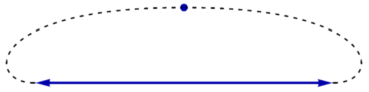
\includegraphics[width=.55\linewidth]{figures/projective-real-line-loop.pdf}\par}

对 $n>1$, 要画出 $\mathbb{P}^{n}$ 的直观图形会更难, 但同样的视角仍然成立. 例如, 有
\[
  \mathbb{P}^{2}_{\mathbb{R}}=\mathbb{A}^{2}_{\mathbb{R}}\sqcup\{\text{无穷远点}\}.
\]
在这个空间中, 可以沿 $\mathbb{A}^{2}_{\mathbb{R}}$ 中任意直线趋向无穷远. 为此, 考虑沿斜率为 $m$, $y$ 轴截距为 $b$ 的直线 $y=mx+b$ 向外延伸的点列 $(1,m+b),(2,2m+b),(3,3m+b),\ldots$. 这些点在 $\mathbb{P}^{2}_{\mathbb{R}}$ 中对应于
\[
  [1:1:m+b],\ [1:2:2m+b],\ [1:3:3m+b],\ldots\in\mathbb{P}^{2}_{\mathbb{R}}.
\]
重新缩放后, 得到等价的点
\[
  \bigl[\tfrac{1}{1}:1:m+\tfrac{b}{1}\bigr],\
  \bigl[\tfrac{1}{2}:1:m+\tfrac{b}{2}\bigr],\
  \bigl[\tfrac{1}{3}:1:m+\tfrac{b}{3}\bigr],\ldots\in\mathbb{P}^{2}_{\mathbb{R}},
\]
它们趋向 $[0:1:m]$. 这个极限是 $\mathbb{P}^{2}_{\mathbb{R}}$ 的一个\textquotedbl{}无穷远点\textquotedbl{}, 因为它的第一个坐标为零. \hyperref[fig:projective-real-plane-infinity]{下图}画出了 $\mathbb{A}^{2}_{\mathbb{R}}$ 和 $\mathbb{P}^{2}_{\mathbb{R}}$ 中沿不同斜率的直线所趋近的几个无穷远点.

\BookPairedFigure
  {现在可以看出, 为什么 $\mathbb{P}^{2}_{\mathbb{R}}$ 有许多无穷远点, 而 $\mathbb{P}^{1}_{\mathbb{R}}$ 只有一个: 在 $\mathbb{P}^{2}_{\mathbb{R}}$ 中沿直线向外走时, 所趋近的无穷远点取决于这条直线的斜率. 实际上, 可以把\textquotedbl{}沿直线走向它所通往的无穷远点\textquotedbl{}的想法精确表述为一个双射: $\mathbb{P}^{2}_{\mathbb{R}}$ 中的无穷远点对应于 $\mathbb{A}^{2}_{\mathbb{R}}$ 中经过原点的直线. 这是一个更一般现象的特例, 下面给出陈述.}
  {\phantomsection\label{fig:projective-real-plane-infinity}%
   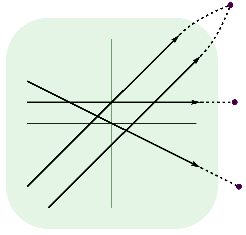
\includegraphics[width=\linewidth]{figures/projective-real-plane-infinity.pdf}}

\begin{Proposition}{无穷远点是直线的斜率}\leavevmode\label{prop:points-at-infinity-correspond-to-lines-through-origin}
对任意 $n\in\mathbb{N}$, 有自然双射
\[
  \{\mathbb{P}^{n}\text{ 中的无穷远点}\}
    =\{\mathbb{A}^{n}\text{ 中经过 }(0,\ldots,0)\text{ 的直线}\}.
\]
\end{Proposition}
\begin{Proof}
按定义, 经过 $(0,\ldots,0)\in\mathbb{A}^{n}$ 的直线是形如
\[
  L=\{(\lambda a_{1},\lambda a_{2},\ldots,\lambda a_{n})\mid\lambda\in K\}
\]
的点集, 其中 $a_{i}\in K$ 固定, 且至少一个 $a_{i}$ 非零. 所需的双射就是把直线
\[
  L=\{(\lambda a_{1},\lambda a_{2},\ldots,\lambda a_{n})\mid\lambda\in K\}
\]
对应到无穷远点
\[
  [0:a_{1}:a_{2}:\cdots:a_{n}]\in\mathbb{P}^{n}.
\]
可将该点看成 $L$ 上向外延伸的点列所趋向的点 (建议读者从直观上验证).
\end{Proof}

由于 $\mathbb{P}^{n}$ 的无穷远点也与 $\mathbb{P}^{n-1}$ 双射, 可以从另一个角度看 Proposition~\ref{prop:points-at-infinity-correspond-to-lines-through-origin}: 它给出了射影空间的第三种视角, 这种视角常被用作射影空间本身的另一种定义.

\begin{Corollary}{射影空间的第三种视角}\leavevmode\label{cor:projective-space-as-lines-through-origin}
对任意 $n\in\mathbb{N}$, 有自然双射
\[
  \mathbb{P}^{n}=\{\mathbb{A}^{n+1}\text{ 中经过 }(0,\ldots,0)\text{ 的直线}\}.
\]
\end{Corollary}

沿 Proposition~\ref{prop:points-at-infinity-correspond-to-lines-through-origin} 的双射追溯, 可以看出怎样将第一种和第三种视角对应起来: 元素 $[a_{0}:a_{1}:\cdots:a_{n}]\in\mathbb{P}^{n}$ 对应于直线
\[
  L=\{(\lambda a_{0},\lambda a_{1},\ldots,\lambda a_{n})\mid\lambda\in K\}\subseteq\mathbb{A}^{n+1},
\]
即经过原点和 $(a_{0},a_{1},\ldots,a_{n})\in\mathbb{A}^{n+1}$ 的直线.

将这些想法合起来, 可以从三种角度看 $\mathbb{P}^{n}$ 的元素: 它是一个等价类 $[a_{0}:a_{1}:\cdots:a_{n}]$, 是 $\mathbb{A}^{n}$ 中的一个点或一个无穷远点, 或者是 $\mathbb{A}^{n+1}$ 中经过原点的一条直线. 根据语境在这些视角之间自如切换, 正是读者在探索射影空间, 以及从下一节开始探索已知的簇的理论在射影空间中的对应理论时, 将逐渐掌握的能力之一.

\BookExerciseHeading
\begin{BookExercises}
  \item\label{ex:compare-projective-coordinate-representatives} 设 $[2:1:3]\in\mathbb{P}^{2}$. 证明
  \[
    [2:1:3]=[6:3:9]
  \]
  但
  \[
    [2:1:3]\neq[6:4:12].
  \]
  一般地, 哪些 $[a:b:c]\in\mathbb{P}^{2}$ 满足 $[2:1:3]=[a:b:c]$?
  \item\label{ex:cross-multiplied-projective-coordinates} 证明 $[a_{0}:\cdots:a_{n}]=[b_{0}:\cdots:b_{n}]\in\mathbb{P}^{n}$ 当且仅当
  \[
    a_{i}b_{j}=a_{j}b_{i}\qquad\text{对所有 }i,j\in\{0,\ldots,n\}.
  \]
  在这种情形, 称交叉相乘的结果相同.
  \item\label{ex:projective-space-affine-part-and-infinity} 分三步证明存在自然双射 $\mathbb{P}^{n}=\mathbb{A}^{n}\sqcup\mathbb{P}^{n-1}$:
  \begin{enumerate}
    \item 定义
    \[
      U=\{[a_{0}:a_{1}:\cdots:a_{n}]\in\mathbb{P}^{n}\mid a_{0}\neq0\}
    \]
    和
    \[
      V=\{[a_{0}:a_{1}:\cdots:a_{n}]\in\mathbb{P}^{n}\mid a_{0}=0\}.
    \]
    证明 $\mathbb{P}^{n}=U\sqcup V$.
    \item 证明 $U$ 与 $\mathbb{A}^{n}$ 之间有自然双射.
    \item 证明 $V$ 与 $\mathbb{P}^{n-1}$ 之间有自然双射.
  \end{enumerate}
  \item\label{ex:projective-space-disjoint-affine-decomposition} 证明存在自然双射
  \[
    \mathbb{P}^{n}=\mathbb{A}^{n}\sqcup\mathbb{A}^{n-1}\sqcup\mathbb{A}^{n-2}
      \sqcup\cdots\sqcup\mathbb{A}^{1}\sqcup\mathbb{A}^{0}
  \]
  并描述每个分量中的点.
  \item\label{ex:projective-point-affine-and-line-perspectives} 设 $[2:1:3]\in\mathbb{P}^{2}$. 将这个点描述成
  \begin{enumerate}
    \item $\mathbb{A}^{2}\sqcup\mathbb{P}^{1}$ 的一个元素;
    \item $\mathbb{A}^{3}$ 中经过 $(0,0,0)$ 的一条直线.
  \end{enumerate}
  \item\label{ex:projective-infinity-point-affine-and-line-perspectives} 对点 $[0:1:3]\in\mathbb{P}^{2}$ 重做 Problem~\ref{ex:projective-point-affine-and-line-perspectives}.
  \item\label{ex:origin-lines-projecting-to-infinity} $\mathbb{A}^{3}$ 中经过 $(0,0,0)$ 的哪些直线对应于 $\mathbb{P}^{2}$ 中的无穷远点?
\end{BookExercises}

\section{\texorpdfstring{射影 $\mathcal{V}$ 算子}{射影 V 算子}}\label{sec:projective-vanishing-operator}

与仿射簇一样, 射影簇也定义为一族多项式的共同零点集. 按 Definition~\ref{def:projective-space-homogeneous-coordinates} 对 $\mathbb{P}^{n}$ 的描述, 这些多项式的输入是元组 $(a_{0},\ldots,a_{n})$. 然而, Definition~\ref{def:projective-space-homogeneous-coordinates} 涉及等价关系, 所以一个多项式可能在一个代表元上取值为零, 而在另一个代表元上不为零. 因此, 多项式在射影空间的一点处\textquotedbl{}取值为零\textquotedbl{}的含义并不显然.

例如, 将 $\mathbb{P}^{1}$ 中形如 $[a_{0}:a_{1}]$ 的点作为二元多项式 $f=x_{0}^{2}-x_{1}$ 的输入. 点 $[2:4]$ 看起来属于 $f$ 的零点集, 因为
\[
  f(2,4)=2^{2}-4=0.
\]
然而, 另一方面, $[2:4]=[4:8]$, 且
\[
  f(4,8)=4^{2}-8=8\neq0.
\]
因此, $f$ 是否在点 $[2:4]=[4:8]$ 处取值为零, 似乎没有一个良定义的答案. 解决这一不一致的方法是规定: 只有当一个多项式在射影空间某点的每个代表元上取值都为零时, 才说它在该点处\textquotedbl{}取值为零\textquotedbl{}.

\begin{Definition}{射影消没}\leavevmode\label{def:projective-vanishing}
设 $f\in K[x_{0},\ldots,x_{n}]$ 为多项式, $a\in\mathbb{P}^{n}$ 为一点. 若对每个代表元 $a=[a_{0}:\cdots:a_{n}]$ 都有
\[
  f(a_{0},\ldots,a_{n})=0,
\]
则称 $f$ \emph{在 $a$ 处取值为零}, 并记为 $f(a)=0$.
\end{Definition}

例如, 多项式 $f(x_{0},x_{1})=x_{0}^{2}-x_{1}$ 在点 $a=[2:4]\in\mathbb{P}^{1}$ 处不为零, 因为它在等价代表元 $a=[4:8]$ 上取值不为零. 乍看之下, 检查多项式是否在一个点的每个代表元上取值都为零, 似乎很费力. 毕竟, 每个点都有无穷多个代表元. 不过, 引入齐次多项式后, 这项工作可以简化.

\begin{Definition}{齐次多项式}\leavevmode\label{def:homogeneous-polynomial}
若多项式 $f\in K[x_{0},\ldots,x_{n}]$ 的每一非零项的次数都是 $d$, 则称 $f$ 是 \emph{$d$ 次齐次多项式}.
\end{Definition}

\begin{BookFlowNote}[l]{%
例如, 二元多项式 $f=x_{0}^{2}-x_{1}$ 是非齐次的, 因为它有一项是非零的二次项, 另一项是非零的一次项; 而 $g=x_{0}^{2}-2x_{0}x_{1}$ 是二次齐次多项式.
}
\noindent $f$ 的一\textquotedbl{}项\textquotedbl{}是表达式 $f=\sum_{\alpha}a_{\alpha}x^{\alpha}$ 中的任何一个加项. 当 $a_{\alpha}\neq0$ 时, 项 $a_{\alpha}x^{\alpha}$ 是\textquotedbl{}非零的\textquotedbl{}.

零多项式没有非零项, 所以它对任何次数都满足齐次性.
\end{BookFlowNote}

在研究射影空间中的消没时, 使用齐次多项式的重要性体现在下面的结果中.

\begin{Lemma}{齐次多项式的射影消没}\leavevmode\label{lem:homogeneous-polynomial-vanishing-on-representatives}
设 $f\in K[x_{0},\ldots,x_{n}]$ 为齐次多项式, 且
\[
  [a_{0}:\cdots:a_{n}]=[b_{0}:\cdots:b_{n}]\in\mathbb{P}^{n}.
\]
则
\[
  f(a_{0},\ldots,a_{n})=0\quad\Longleftrightarrow\quad f(b_{0},\ldots,b_{n})=0.
\]
\end{Lemma}

换句话说, 对齐次多项式, 只须检查它在一个代表元上的取值是否为零. 例如, 考虑齐次多项式 $g=x_{0}^{2}-2x_{0}x_{1}$. 要验证 $g$ 在等价类 $[2:1]\in\mathbb{P}^{1}$ 处取值为零, 只须验证一个代表元:
\[
  g(2,1)=2^{2}-2\cdot2\cdot1=0.
\]
若把 $[2:1]$ 换成另一个代表元 $[4:2]$ (或 $\mathbb{P}^{1}$ 中这个点的任一其他代表元), 取值仍为零:
\[
  g(4,2)=4^{2}-2\cdot4\cdot2=0.
\]

\begin{Proof}\textbf{of Lemma~\ref{lem:homogeneous-polynomial-vanishing-on-representatives}.}\quad
所需的关键观察是, $f$ 为 $d$ 次齐次多项式当且仅当对所有 $\lambda,a_{0},\ldots,a_{n}\in K$, 有
\begin{equation}\label{eq:homogeneous-polynomial-scaling}
  f(\lambda a_{0},\ldots,\lambda a_{n})=\lambda^{d}f(a_{0},\ldots,a_{n})
\end{equation}
(Exercise~\ref{ex:characterize-homogeneous-polynomials-by-scaling}). 设 $f$ 为 $d$ 次齐次多项式, 且
\[
  [a_{0}:\cdots:a_{n}]=[b_{0}:\cdots:b_{n}]\in\mathbb{P}^{n}.
\]
按 $\mathbb{P}^{n}$ 上等价关系的定义, 存在非零的 $\lambda\in K$, 使得
\[
  (\lambda a_{0},\ldots,\lambda a_{n})=(b_{0},\ldots,b_{n}).
\]
由 \eqref{eq:homogeneous-polynomial-scaling} 可见, $f(b_{0},\ldots,b_{n})$ 与 $f(a_{0},\ldots,a_{n})$ 相差非零的标量倍数 $\lambda^{d}$, 所以一个为零当且仅当另一个为零.
\end{Proof}

Lemma~\ref{lem:homogeneous-polynomial-vanishing-on-representatives} 表明, 只须检查一个代表元, 便可判定齐次多项式是否在射影空间的一点处取值为零. 但非齐次多项式又如何? 为回答这个问题, 我们引入多项式的齐次分量.

\begin{Definition}{齐次分量}\leavevmode\label{def:homogeneous-components}
给定多项式 $f\in K[x_{0},\ldots,x_{n}]$, $f$ 的 \emph{$d$ 次齐次分量}记为 $f_{d}$, 是 $f$ 的所有 $d$ 次非零项之和. 若 $f$ 没有 $d$ 次非零项, 则 $f_{d}=0$.
\end{Definition}

例如, 多项式
\[
  f=x^{4}z+x^{2}y+xyz+x+y+5
\]
的非零齐次分量是
\[
  f_{5}=x^{4}z,\quad f_{3}=x^{2}y+xyz,\quad f_{1}=x+y,\quad f_{0}=5.
\]
下一个结果用齐次分量的消没来刻画多项式在射影空间一点处的消没.

\begin{Lemma}{射影消没与齐次分量}\leavevmode\label{lem:projective-vanishing-of-components}
设 $f\in K[x_{0},\ldots,x_{n}]$ 是多项式, $a\in\mathbb{P}^{n}$ 为一点. 则 $f$ 在 $a$ 处取值为零当且仅当 $f$ 的每个齐次分量都在 $a$ 处取值为零.
\end{Lemma}

换句话说, 为判定一般的多项式是否在 $\mathbb{P}^{n}$ 中一点 (的每个代表元) 处取值为零, 由 Lemmas~\ref{lem:homogeneous-polynomial-vanishing-on-representatives} 和~\ref{lem:projective-vanishing-of-components}, 只须检查每个齐次分量在该点的一个代表元上是否都取值为零.

\begin{Proof}\textbf{of Lemma~\ref{lem:projective-vanishing-of-components}.}\quad
设 $f\in K[x_{0},\ldots,x_{n}]$ 是 $d$ 次多项式. 它可写成次数 $\leq d$ 的各齐次分量之和:
\begin{equation}\label{eq:polynomial-sum-of-homogeneous-components}
  f=\sum_{k=0}^{d}f_{k}.
\end{equation}
若每个 $f_{k}$ 在点 $a$ 的每个代表元上取值都为零, 则由 \eqref{eq:polynomial-sum-of-homogeneous-components}, $f$ 在 $a$ 的每个代表元上取值都为零.

反过来, 假设 $f$ 在 $a$ 的每个代表元上取值都为零. 选定一个代表元 $a=[a_{0}:\cdots:a_{n}]$. 那么对任意 $\lambda\in K\setminus\{0\}$, 有
\[
  \begin{aligned}
    0=f(\lambda a_{0},\ldots,\lambda a_{n})
      &=\sum_{k=0}^{d}f_{k}(\lambda a_{0},\ldots,\lambda a_{n})\\
      &=\sum_{k=0}^{d}\lambda^{k}f_{k}(a_{0},\ldots,a_{n}),
  \end{aligned}
\]
其中第二个等号用了 \eqref{eq:homogeneous-polynomial-scaling}. 换句话说, 一元多项式
\[
  \sum_{k=0}^{d}x^{k}f_{k}(a_{0},\ldots,a_{n})\in K[x]
\]
在 $K$ 中无穷多个值处取值为零, 故必为零多项式. 于是对所有 $k$, 都有 $f_{k}(a_{0},\ldots,a_{n})=0$. 由于 $f_{k}$ 齐次, Lemma~\ref{lem:homogeneous-polynomial-vanishing-on-representatives} 蕴含每个 $f_{k}$ 在 $a$ 的每个代表元上取值都为零.
\end{Proof}

更清楚地理解了多项式在射影空间的点处取值为零的含义之后, 现在给出射影簇的自然定义.

\begin{Definition}{射影 $\mathcal{V}$ 算子}\leavevmode\label{def:projective-vanishing-operator}
设 $S\subseteq K[x_{0},\ldots,x_{n}]$ 为多项式集合. $S$ 的\emph{射影零点集}是
\[
  \mathcal{V}_{\mathbb{P}}(S)=\{a\in\mathbb{P}^{n}\mid f(a)=0\text{ 对所有 }f\in S\}.
\]
若子集 $X\subseteq\mathbb{P}^{n}$ 对某个集合 $S\subseteq K[x_{0},\ldots,x_{n}]$ 满足 $X=\mathcal{V}_{\mathbb{P}}(S)$, 则称 $X$ 为\emph{射影簇}.
\end{Definition}

\begin{BookFlowNote}[l]{%
由 Lemma~\ref{lem:projective-vanishing-of-components}, 只须把 $S$ 中的非齐次多项式换成它们的齐次分量, 就能用一组齐次多项式描述每个射影簇.
}
\noindent 当由语境可清楚看出是在射影空间, 而非仿射空间中讨论时, 常写作 $\mathcal{V}(S)\subseteq\mathbb{P}^{n}$.

因此, 通常把射影簇描述为一族齐次多项式的零点集. 来看几个例子.
\end{BookFlowNote}

\begin{Example}{$\varnothing$ 和 $\mathbb{P}^{n}$ 是射影簇}\leavevmode\label{ex:empty-set-and-projective-space-are-projective-varieties}
与仿射情形一样, $\mathcal{V}(1)=\varnothing$ 且 $\mathcal{V}(0)=\mathbb{P}^{n}$, 所以 $\varnothing$ 和 $\mathbb{P}^{n}$ 都是射影簇.
\end{Example}

\begin{Example}{$\mathbb{P}^{1}$ 中的射影簇}\leavevmode\label{ex:projective-varieties-in-projective-line}
在 $\mathbb{P}^{1}$ 中, 考虑射影簇
\[
  X=\mathcal{V}(2x_{0}-x_{1})
   =\{[a_{0}:a_{1}]\in\mathbb{P}^{1}\mid 2a_{0}-a_{1}=0\}.
\]
$X$ 中的点 $[a_{0}:a_{1}]$ 不能满足 $a_{0}=0$, 否则方程 $2a_{0}-a_{1}=0$ 会迫使 $a_{1}$ 也为零. 因此
\[
  X=\{[a:2a]\in\mathbb{P}^{1}\mid a\in K\setminus\{0\}\}=\{[1:2]\},
\]
因为将两个坐标同时乘以 $a^{-1}$ 可知, 对任意 $a$, 有 $[a:2a]=[1:2]$. 更一般地, 与 $\mathbb{A}^{1}$ 的情形完全类似, $\mathbb{P}^{1}$ 中的任意射影簇要么是整个 $\mathbb{P}^{1}$, 要么是有限 (可能为空) 的点集 (Exercise~\ref{ex:classify-varieties-in-projective-line}).
\end{Example}

\begin{Example}{$\mathbb{P}^{2}$ 中的一条直线}\leavevmode\label{ex:projective-line-in-projective-plane}
在 $\mathbb{P}^{2}$ 中, 考虑射影簇
\[
  X=\mathcal{V}(x_{0}+x_{1}-x_{2})
   =\{[a_{0}:a_{1}:a_{2}]\in\mathbb{P}^{2}\mid a_{0}+a_{1}-a_{2}=0\}.
\]
$X$ 中的点 $[a_{0}:a_{1}:a_{2}]$ 不能满足 $a_{0}=a_{1}=0$, 否则定义方程会迫使 $a_{2}$ 也为零. 从而
\[
  X=\{[a_{0}:a_{1}:a_{0}+a_{1}]\in\mathbb{P}^{2}\mid a_{0},a_{1}\in K\text{ 不全为 }0\}.
\]
由此不难看出, $\mathcal{V}(x_{0}+x_{1}-x_{2})$ 的点与 $\mathbb{P}^{1}$ 有双射.

与仿射情形类似, 在 $\mathbb{A}^{2}$ 中线性多项式的零点集描述一条直线, 我们称 $X$ 为 $\mathbb{P}^{2}$ 中的一条直线. 这个直观的术语不宜完全照字面理解: 如上一节所见, 射影\textquotedbl{}直线\textquotedbl{}实际上不像平面几何中熟悉的直线. 即使在实数域上也是如此, 此时射影直线形成一个环.
\end{Example}

要利用多项式环的代数结构研究射影簇, 第一步是注意每个射影簇都可由一个理想定义. 这个结果与仿射情形中的 Proposition~\ref{prop:affine-varieties-defined-by-ideals} 对应.

\begin{Proposition}{射影簇可由理想定义}\leavevmode\label{prop:projective-varieties-defined-by-ideals}
若 $S\subseteq K[x_{0},\ldots,x_{n}]$ 为多项式集合, 则
\[
  \mathcal{V}_{\mathbb{P}}(S)=\mathcal{V}_{\mathbb{P}}(\langle S\rangle).
\]
\end{Proposition}
\begin{Proof}
见 Exercise~\ref{ex:projective-vanishing-of-generated-ideal}.
\end{Proof}

和仿射情形一样, 知道每个射影簇都可由一个理想定义后, 就能利用多项式环的代数结构推出, 每个射影簇都可由有限多个多项式定义. 而且, 在射影情形还能进一步利用 Lemma~\ref{lem:projective-vanishing-of-components} 推出, 每个射影簇都是一组有限个齐次多项式的零点集.

\begin{Corollary}{射影簇可由有限个多项式定义}\leavevmode\label{cor:projective-varieties-defined-by-finite-homogeneous-set}
任意射影簇 $X\subseteq\mathbb{P}^{n}$ 都具有形式
\[
  X=\mathcal{V}_{\mathbb{P}}(f_{1},\ldots,f_{k}),
\]
其中 $f_{1},\ldots,f_{k}\in K[x_{0},\ldots,x_{n}]$ 为齐次多项式.
\end{Corollary}
\begin{Proof}
见 Exercise~\ref{ex:finite-homogeneous-equations-for-projective-variety}.
\end{Proof}

到这里, 已可看出用射影簇的定义理想, 而非仅用多项式集合来作代数研究的好处. 特别地, 正是通过转到理想并应用多项式环的 Hilbert 基定理, 才能证明 Corollary~\ref{cor:projective-varieties-defined-by-finite-homogeneous-set}. 和仿射情形一样, 一个射影簇可以有许多定义理想, 但总有一个特别的定义理想, 即消没理想. 下一节转而讨论射影情形中的消没理想.

\BookExerciseHeading
\begin{BookExercises}
  \item\label{ex:characterize-homogeneous-polynomials-by-scaling} 设 $f\in K[x_{0},x_{1},\ldots,x_{n}]$ 为非零多项式. 证明 $f$ 为 $d$ 次齐次多项式当且仅当对任意 $\lambda,a_{0},a_{1},\ldots,a_{n}\in K$, 都有
  \[
    f(\lambda a_{0},\lambda a_{1},\ldots,\lambda a_{n})=\lambda^{d}f(a_{0},a_{1},\ldots,a_{n}).
  \]
  \item\label{ex:classify-varieties-in-projective-line} 证明 $\mathbb{P}^{1}$ 中的射影簇只有 $\mathbb{P}^{1}$ 本身和有限点集.
  \item\label{ex:projective-vanishing-of-generated-ideal} 证明 Proposition~\ref{prop:projective-varieties-defined-by-ideals}.
  \item\label{ex:finite-homogeneous-equations-for-projective-variety} 证明 Corollary~\ref{cor:projective-varieties-defined-by-finite-homogeneous-set}.
  \item\label{ex:projective-varieties-closed-under-unions-and-intersections} 证明射影簇的有限并和任意交都是射影簇.
  \item\label{ex:projective-conic-and-affine-chart} 令
  \[
    X=\mathcal{V}(x_{0}x_{1}-x_{2}^{2})\subseteq\mathbb{P}^{2}.
  \]
  \begin{enumerate}
    \item 令 $U=\{[a_{0}:a_{1}:a_{2}]\in\mathbb{P}^{2}\mid a_{0}\neq0\}$. 由上一节的结论, 它与 $\mathbb{A}^{2}$ 有自然双射. 证明这一双射将 $X\cap U$ 与 $\mathbb{A}^{2}$ 中的一个仿射簇认同. 这是哪个仿射簇? 画出 $X\cap U$ 在 $\mathbb{R}$ 上的图形.
    \item 求 $X\setminus U$ 的所有点, 并描述 (b) 中找到的仿射簇里的点如何趋近这些点.
    \item 描述 $X$ 与 $\mathbb{P}^{1}$ 之间的一个双射.
  \end{enumerate}
  \item\label{ex:projective-conic-with-other-affine-chart} 对 $X=\mathcal{V}(x_{0}^{2}-x_{1}x_{2})\subseteq\mathbb{P}^{2}$ 完成上一题.
\end{BookExercises}

\par\medskip
{\footnotesize
\noindent\textbf{开放获取.} 本章按照
\href{http://creativecommons.org/licenses/by-nc/4.0/}{Creative Commons Attribution-NonCommercial 4.0 International License}
的条款授权. 该许可允许以任何媒介或格式进行非商业性使用, 分享, 改编, 分发和复制, 但须对原作者和来源作适当署名, 提供 Creative Commons 许可的链接, 并说明是否作了修改.

\noindent
\begin{minipage}[t]{.17\linewidth}
  \vspace{0pt}
\includegraphics[width=.9\linewidth]{figures/source-cc-by-nc.png}
\end{minipage}\hfill
\begin{minipage}[t]{.81\linewidth}
  \vspace{0pt}本章的图片或其他第三方材料均纳入本章的 Creative Commons 许可, 除非材料的署名行另有注明. 如果材料未纳入本章的 Creative Commons 许可, 且您拟进行的使用未获法律规定的许可或超出允许使用的范围, 则须直接向著作权持有人取得许可.
\end{minipage}\par}

\section{\texorpdfstring{射影 $\mathcal{I}$ 算子}{射影 I 算子}}\label{sec:projective-ideal-operator}

射影 $\mathcal{V}$ 算子使我们从多项式集合转到射影空间的子集. 现在转向射影 $\mathcal{I}$ 算子, 它沿相反的方向作用. $\mathcal{I}_{\mathbb{P}}$ 的定义正如所料.

\begin{Definition}{射影 $\mathcal{I}$ 算子}\leavevmode\label{def:projective-ideal-operator}
设 $X\subseteq\mathbb{P}^{n}$ 为子集. $X$ 的\emph{消没理想}是
\[
  \mathcal{I}_{\mathbb{P}}(X)=
    \{f\in K[x_{0},\ldots,x_{n}]\mid f(a)=0\text{ 对所有 }a\in X\}.
\]
若 $K[x_{0},\ldots,x_{n}]$ 的子集对某个 $X\subseteq\mathbb{P}^{n}$ 形如 $\mathcal{I}_{\mathbb{P}}(X)$, 则称它为\emph{射影消没理想}.
\end{Definition}

\begin{BookFlowNote}[l]{%
回顾 Definition~\ref{def:projective-vanishing}, 当我们说 $f(a)=0$ 时, 是指 $f$ 在点 $a\in\mathbb{P}^{n}$ 的每个代表元上取值都为零. 例如, 若 $[1:0]$ 是 $X$ 的一点, 那么多项式 $f=x_{0}-1$ 不属于 $\mathcal{I}(X)$.
}
\noindent 与 $\mathcal{V}_{\mathbb{P}}$ 算子一样, 当由语境可清楚看出是在仿射空间还是射影空间中讨论时, 常写作 $\mathcal{I}(X)$.

尽管 $f(1,0)=0$, 但 $f$ 在代表元 $[2:0]=[1:0]$ 上取值不为零. 下一个例子进一步说明这一点.
\end{BookFlowNote}

\begin{Example}{$\mathbb{P}^{1}$ 中一点的消没理想}\leavevmode\label{ex:vanishing-ideal-of-point-in-projective-line}
令 $X=\{[1:0]\}\subseteq\mathbb{P}^{1}$. 那么 $f=x_{1}\in K[x_{0},x_{1}]$ 是 $\mathcal{I}(X)$ 的元素, 因为点 $[1:0]\in X$ 的任意代表元对某个 $a$ 都形如 $[a:0]$, 而对任意 $a$ 都有 $f(a,0)=0$. 更一般地, 有 $\langle x_{1}\rangle\subseteq\mathcal{I}(X)$. 实际上我们断言等号成立: $\mathcal{I}(X)=\langle x_{1}\rangle$.

为证明反向包含, 令 $f\in\mathcal{I}(X)$. 那么对所有非零 $a\in K$, 有 $f(a,0)=0$. 因此, $f(x_{0},0)$ 是有无穷多个零点的一元多项式, 必为零多项式. 把 $f$ 写成 $(K[x_{0}])[x_{1}]$ 的元素:
\[
  f=\sum_{d\geq0}f_{d}(x_{0})x_{1}^{d}.
\]
由 $f_{0}(x_{0})=f(x_{0},0)=0$, 可得
\[
  f=x_{1}\sum_{d\geq1}f_{d}(x_{0})x_{1}^{d-1}\in\langle x_{1}\rangle.
\]
\end{Example}

\begin{Example}{$\mathbb{P}^{2}$ 中一条直线的消没理想}\leavevmode\label{ex:vanishing-ideal-of-projective-line-in-plane}
若 $X$ 是 Example~\ref{ex:projective-line-in-projective-plane} 中的直线 $\mathcal{V}(x_{0}+x_{1}-x_{2})\subseteq\mathbb{P}^{2}$, 则
\[
  \mathcal{I}(X)=\langle x_{0}+x_{1}-x_{2}\rangle.
\]
$\langle x_{0}+x_{1}-x_{2}\rangle$ 中每个元素在 $X$ 的每一点处取值都为零, 这基本上是直接的. 而反向包含是 Exercise~\ref{ex:vanishing-ideal-of-projective-line-by-substitution} 的内容.
\end{Example}

与仿射情形一样, 射影消没理想确实是理想, 并且容易看出它们是根理想. 不过, 在射影情形还能进一步得到: Lemma~\ref{lem:projective-vanishing-of-components} 蕴含, 对每个 $f\in\mathcal{I}(X)$, $f$ 的每个齐次分量也必属于 $\mathcal{I}(X)$. $\mathcal{I}(X)$ 的这一性质正是齐次理想的定义性质.

\begin{Definition}{齐次理想}\leavevmode\label{def:homogeneous-ideal}
若对理想 $I\subseteq K[x_{0},\ldots,x_{n}]$ 中每个 $f\in I$, $f$ 的每个齐次分量也属于 $I$, 则称 $I$ 是\emph{齐次理想}.
\end{Definition}

上述齐次理想的定义直接来自对消没理想的讨论, 而下面的结果给出齐次理想的另一种重要刻画. 这种刻画或许更直接, 在实践中也很有用.

\begin{Proposition}{齐次理想的刻画}\leavevmode\label{prop:homogeneous-ideal-has-homogeneous-generators}
理想 $I\subseteq K[x_{0},\ldots,x_{n}]$ 是齐次的当且仅当它有一组齐次生成元.
\end{Proposition}
\begin{Proof}
先设 $I$ 是齐次理想, 并令 $S\subseteq I$ 为 $I$ 中所有齐次多项式组成的子集. 只须证明 $I=\langle S\rangle$. 由于 $S\subseteq I$ 且 $I$ 是理想, 有 $\langle S\rangle\subseteq I$. 为证明反向包含, 设 $f\in I$. 那么可将 $f$ 写成非零齐次分量 $f_{k}$ 之和. $I$ 是齐次理想, 所以每个 $f_{k}\in I$. 又由于 $f_{k}$ 齐次, 可知 $f_{k}\in S$. 因此 $f$ 是 $S$ 中元素之和, 即 $f\in\langle S\rangle$. 从而 $I=\langle S\rangle$, 如所断言.

反过来, 设 $I=\langle S\rangle$, 其中 $S$ 是一组齐次多项式. 为证明 $I$ 为齐次理想, 令 $f\in I$. 由 $I=\langle S\rangle$, 可知
\[
  f=\sum_{i=1}^{m}g_{i}h_{i}
\]
其中 $g_{i}\in K[x_{0},\ldots,x_{n}]$ 且 $h_{i}\in S$. 特别地, $h_{i}$ 是某个次数 $d_{i}$ 的齐次多项式. 对每个 $k$, 有
\[
  f_{k}=\sum_{i=1}^{m}(g_{i}h_{i})_{k},
\]
其中右侧的 $(g_{i}h_{i})_{k}$ 表示多项式 $g_{i}h_{i}$ 的 $k$ 次齐次分量. 由 Exercise~\ref{ex:homogeneous-component-of-product-with-homogeneous-factor}, 可以将各加项写成
\[
  (g_{i}h_{i})_{k}=
  \begin{cases}
    (g_{i})_{k-d_{i}}\cdot h_{i} & \text{若 }d_{i}\leq k,\\
    0 & \text{若 }d_{i}>k,
  \end{cases}
\]
其中 $(g_{i})_{k-d_{i}}$ 是 $g_{i}$ 的 $(k-d_{i})$ 次齐次分量. 这蕴含 $(g_{i}h_{i})_{k}\in I$, 因为它是 $h_{i}\in S$ 的倍式. 所以 $f_{k}$ 是 $I$ 中元素之和, 从而 $f_{k}\in I$. 这就证明 $I$ 是齐次理想.
\end{Proof}

理解了齐次理想后, 现在回到本节的主要话题: 消没理想. 下一个结果概括了射影消没理想最重要的代数性质.

\begin{Proposition}{$\mathcal{I}_{\mathbb{P}}(X)$ 是齐次根理想}\leavevmode\label{prop:projective-vanishing-ideal-is-homogeneous-radical}
若 $X\subseteq\mathbb{P}^{n}$ 是任意子集, 则 $\mathcal{I}_{\mathbb{P}}(X)\subseteq K[x_{0},\ldots,x_{n}]$ 是齐次根理想.
\end{Proposition}
\begin{Proof}
$\mathcal{I}_{\mathbb{P}}(X)$ 是根理想的事实, 可以用与仿射情形 (Proposition~\ref{prop:vanishing-ideals-are-radical}) 完全相同的论证得出, 建议读者自行验证. $\mathcal{I}(X)$ 是齐次的, 则按定义由 Lemma~\ref{lem:projective-vanishing-of-components} 得出.
\end{Proof}

和仿射情形一样, 定义消没理想的主要理由是, 为每个射影簇选出一个特别的定义理想. 下一个结果的第三项验证了消没理想的这一作用. 它只是联系射影 $\mathcal{V}$ 和 $\mathcal{I}$ 算子的若干重要性质之一.

\begin{Proposition}{$\mathcal{V}_{\mathbb{P}}$ 和 $\mathcal{I}_{\mathbb{P}}$ 的基本性质}\leavevmode\label{prop:basic-properties-of-projective-vanishing-operators}
设 $S,T\subseteq K[x_{0},\ldots,x_{n}]$ 和 $X,Y\subseteq\mathbb{P}^{n}$ 为子集.
\begin{enumerate}
  \item 若 $S\subseteq T$, 则 $\mathcal{V}_{\mathbb{P}}(S)\supseteq\mathcal{V}_{\mathbb{P}}(T)$.
  \item 若 $X\subseteq Y$, 则 $\mathcal{I}_{\mathbb{P}}(X)\supseteq\mathcal{I}_{\mathbb{P}}(Y)$.
  \item $\mathcal{V}_{\mathbb{P}}(\mathcal{I}_{\mathbb{P}}(X))\supseteq X$, 等号成立当且仅当 $X$ 为射影簇.
  \item $\mathcal{I}_{\mathbb{P}}(\mathcal{V}_{\mathbb{P}}(S))\supseteq S$, 等号成立当且仅当 $S$ 为射影消没理想.
\end{enumerate}
\end{Proposition}
\begin{Proof}
这些陈述的证明与仿射情形中相应陈述的证明类似 (Propositions~\ref{prop:operators-reverse-inclusions} 和~\ref{prop:compose-vanishing-operators}), 建议读者自行验证.
\end{Proof}

继续与仿射情形作比较. 回忆, 在仿射情形, 我们利用 $\mathcal{V}$ 和 $\mathcal{I}$ 算子间的关系证明了不可约分解的存在性和唯一性. 现在陈述射影情形中相应的结论, 从不可约射影簇的自然定义开始. 这个定义从仿射情形原样沿用.

\begin{Definition}{不可约射影簇}\leavevmode\label{def:irreducible-projective-variety}
若射影簇 $X\subseteq\mathbb{P}^{n}$ 对某些射影簇 $X_{1},X_{2}\subsetneq X$ 满足 $X=X_{1}\cup X_{2}$, 则称 $X$ \emph{可约}. 若 $X$ 既不是空集, 也不是可约簇, 则称 $X$ \emph{不可约}.
\end{Definition}

正如可以预料的那样, 在射影情形, 不可约分解总是存在且唯一, 证明与仿射情形类似.

\begin{BookPropositionDefinition}{不可约分解}\leavevmode\label{prop:projective-irreducible-decomposition}
设 $X\subseteq\mathbb{P}^{n}$ 为非空射影簇. 则存在不可约射影簇 $X_{1},\ldots,X_{r}\subseteq X$, 使得对任意 $i\neq j$ 有 $X_{i}\not\subseteq X_{j}$, 且
\begin{equation}\label{eq:decomposition-into-projective-irreducible-components}
  X=\bigcup_{i=1}^{r}X_{i}.
\end{equation}
此外, 在不计排列顺序的意义下, 这些不可约射影簇 $X_{1},\ldots,X_{r}$ 是唯一的. 称它们为 $X$ 的\emph{不可约分支}, 称 \eqref{eq:decomposition-into-projective-irreducible-components} 为 $X$ 的\emph{不可约分解}.
\end{BookPropositionDefinition}
\begin{Proof}
证明用到射影 $\mathcal{V}$ 和 $\mathcal{I}$ 算子间的关系, 以及 $K[x_{0},\ldots,x_{n}]$ 的 Noether 性质, 与仿射情形的陈述 (Proposition/Definition~\ref{prop:irreducible-decomposition}) 的证明类似. 把验证留给读者作为练习.
\end{Proof}

现在, 射影簇和仿射簇在结构上的相似性已经开始显现. 射影情形中的不少结果, 其证明确实与仿射情形相同或至少类似. 然而, 我们对射影簇还缺乏几何直观. 毕竟, 即使在实数域上, $n\geq2$ 时也很难想象 $\mathbb{P}^{n}$ 的样子, 又如何画出射影簇的图形? 回答这个问题的关键是两种在射影情形和仿射情形之间转换的方法: 仿射限制与射影闭包. 接下来两节专门讨论这两种方法.

\BookExerciseHeading
\begin{BookExercises}
  \item\label{ex:vanishing-ideal-of-projective-line-by-substitution} 令 $X=\mathcal{V}(x_{0}+x_{1}-x_{2})\subseteq\mathbb{P}^{2}$. 我们证明 $\mathcal{I}(X)=\langle x_{0}+x_{1}-x_{2}\rangle$. 如 Example~\ref{ex:vanishing-ideal-of-projective-line-in-plane} 所述, 只须证明 $\mathcal{I}(X)\subseteq\langle x_{0}+x_{1}-x_{2}\rangle$.
  \begin{enumerate}
    \item 令 $f\in\mathcal{I}(X)$. 证明 $f(x_{0},x_{1},x_{0}+x_{1})=0\in K[x_{0},x_{1}]$.
    \item 论证, 由 $f(x_{0},x_{1},x_{0}+x_{1})=0$ 可得 $f\in\langle x_{0}+x_{1}-x_{2}\rangle$.
  \end{enumerate}
  \item\label{ex:homogeneous-component-of-product-with-homogeneous-factor} 令 $g\in K[x_{0},\ldots,x_{n}]$ 为任意多项式, 且令 $h\in[x_{0},\ldots,x_{n}]$ 为 $d$ 次齐次多项式. 证明对每个 $k\geq0$, 有
  \[
    (gh)_{k}=
    \begin{cases}
      g_{k-d}\cdot h & \text{若 }d\leq k,\\
      0 & \text{若 }d>k,
    \end{cases}
  \]
  其中 $(gh)_{k}$ 是 $gh$ 的 $k$ 次齐次分量, 而 $g_{k-d}$ 是 $g$ 的 $(k-d)$ 次齐次分量.
  \item\label{ex:identify-homogeneous-ideals-in-two-variables} $K[x,y]$ 中下列哪些理想是齐次的?
  \begin{enumerate}
    \item $\langle x+1,y^{2}\rangle$
    \item $\langle x+y,x^{2}\rangle$
    \item $\langle x^{2}+y,x^{2}-y\rangle$
    \item $\langle x^{2}+y^{2},xy^{2}+y^{3}+x^{2},y^{2}-x^{2}\rangle$
  \end{enumerate}
  \item\label{ex:principal-ideal-homogeneous-iff-generator-homogeneous} 证明主理想 $\langle f\rangle\subseteq K[x_{0},\ldots,x_{n}]$ 是齐次的当且仅当多项式 $f$ 是齐次的.
  \item\label{ex:projective-irreducibility-equivalent-to-prime-ideal} 设 $X\subseteq\mathbb{P}^{n}$ 为射影簇. 证明 $X$ 不可约当且仅当 $\mathcal{I}_{\mathbb{P}}(X)$ 为素理想.
  \item\label{ex:projective-single-point-equivalent-to-maximal-ideal} 证明子集 $X\subseteq\mathbb{P}^{n}$ 只含一个点当且仅当 $\mathcal{I}_{\mathbb{P}}(X)$ 为极大理想.
  \item\label{ex:adapt-affine-proof-of-radical-ideal-to-projective-space} 用射影簇的语言和记号改写 Proposition~\ref{prop:vanishing-ideals-are-radical} 的证明, 确保每一步都能在射影情形下完成, 从而证明射影消没理想是根理想.
  \item\label{ex:adapt-affine-proof-of-operator-properties-to-projective-space} 用射影簇的语言和记号改写 Propositions~\ref{prop:operators-reverse-inclusions} 和~\ref{prop:compose-vanishing-operators} 的证明, 确保每一步都能在射影情形下完成, 从而证明 Proposition~\ref{prop:basic-properties-of-projective-vanishing-operators}.
  \item\label{ex:adapt-affine-proof-of-decomposition-to-projective-space} 用射影簇的语言和记号改写 Proposition/Definition~\ref{prop:irreducible-decomposition} 的证明, 确保每一步都能在射影情形下完成, 从而证明 Proposition/Definition~\ref{prop:projective-irreducible-decomposition}.
\end{BookExercises}

\section{仿射限制}\label{sec:affine-restrictions}

为了把射影簇与更容易画出图形的仿射簇联系起来, 回顾 Section~\ref{sec:projective-space} 中射影空间的第二种视角: 把 $\mathbb{P}^{n}$ 看成向 $\mathbb{A}^{n}$ 添加无穷远点得到的空间. 略去这些无穷远点, 就能为每个射影簇找到一个仿射限制. 这种限制为我们提供了射影簇的一幅有用但不完整的图景. 在解释一般概念前, 先看一个具体例子.

\begin{Example}{$\mathbb{P}^{2}$ 中一条二次曲线的仿射限制}\leavevmode\label{ex:affine-restriction-of-projective-conic}
\BookPairedNote
  {考虑射影簇
  \[
    X=\mathcal{V}_{\mathbb{P}}(x_{0}^{2}+x_{1}^{2}-x_{2}^{2})\subseteq\mathbb{P}_{\mathbb{C}}^{2}.
  \]
  $X$ 中任何第一个坐标非零的点, 都可用齐次坐标表示为 $[1:a_{1}:a_{2}]$, 其中 $1+a_{1}^{2}-a_{2}^{2}=0$.}
  {同时涉及仿射簇和射影簇时, 常用记号 $\mathcal{V}_{\mathbb{A}}$ 和 $\mathcal{I}_{\mathbb{A}}$ 表示仿射 $\mathcal{V}$ 和 $\mathcal{I}$ 算子, 以区别于相应的射影算子.}
因此, 令
\[
  X_{0}=\mathcal{V}_{\mathbb{A}}(1+x_{1}^{2}-x_{2}^{2})\subseteq\mathbb{A}_{\mathbb{C}}^{2},
\]
则有自然双射
\[
  X=X_{0}\sqcup\{[0:a_{1}:a_{2}]\mid a_{1}^{2}-a_{2}^{2}=0\}.
\]
第二类点有两个: 满足
\[
  0=a_{1}^{2}-a_{2}^{2}=(a_{1}-a_{2})(a_{1}+a_{2})
\]
的点 $[0:a_{1}:a_{2}]\in\mathbb{P}_{\mathbb{C}}^{2}$ 必形如 $[0:a:a]$ 或 $[0:a:-a]$. 按 $\mathbb{P}_{\mathbb{C}}^{2}$ 上的等价关系, 它必等于 $[0:1:1]$ 或 $[0:1:-1]$. 因此
\[
  X=X_{0}\sqcup\{[0:1:1],[0:1:-1]\}.
\]

\BookPairedFigure
  {限制到实数域, 可以画出仿射簇 $X_{0}$: 它是\hyperref[fig:projective-hyperbola-loop]{右图}所示的双曲线, 几乎囊括了整个 $X$. $X$ 中另外两点是沿 $X_{0}$ 的两条渐近线走到的无穷远点. 具体而言, $X_{0}$ 的两条渐近线是过原点且斜率分别为 $1$ 和 $-1$ 的直线.}
  {\phantomsection\label{fig:projective-hyperbola-loop}%
   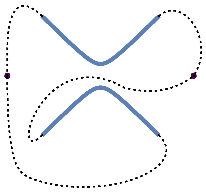
\includegraphics[width=\linewidth]{figures/projective-hyperbola-loop.pdf}}
如 Proposition~\ref{prop:projective-space-affine-plus-infinity} 后的讨论所示, 它们分别趋向 $\mathbb{P}^{2}$ 中的点 $[0:1:1]$ 和 $[0:1:-1]$. 如图所示, 沿着 $X_{0}$ 和两个无穷远点组成的路径走, 可以看到整个射影簇 $X$ 的实点组成一个环, 就像 $\mathbb{P}_{\mathbb{R}}^{1}$. 实际上, 讨论过射影簇的同构之后, 我们将看到存在同构 $X\cong\mathbb{P}_{\mathbb{C}}^{1}$.
\end{Example}

推广 Example~\ref{ex:affine-restriction-of-projective-conic}, 若 $X=\mathcal{V}_{\mathbb{P}}(S)\subseteq\mathbb{P}^{n}$ 为射影簇, 则
\[
  X=X_{0}\sqcup\{X\text{ 中的无穷远点}\},
\]
其中
\[
  X_{0}=\{[a_{0}:\cdots:a_{n}]\in X\mid a_{0}\neq0\},
\]
而 $X$ 中的无穷远点正是满足 $a_{0}=0$ 的那些点. 也就是说, 在 $\mathbb{A}^{n}$ 与 $\mathbb{P}^{n}$ 中第一个坐标非零的点之间的自然双射下, 有 $X_{0}=X\cap\mathbb{A}^{n}$. 由于 $X_{0}$ 中的点可写成 $[1:b_{1}:\cdots:b_{n}]$, 可见
\[
  X_{0}=\mathcal{V}_{\mathbb{A}}(S_{0})\subseteq\mathbb{A}^{n},
\]
其中
\[
  S_{0}=\{f(1,x_{1},\ldots,x_{n})\mid f\in S\}\subseteq K[x_{1},\ldots,x_{n}].
\]
特别地, $X_{0}$ 是仿射簇, 称为 $X$ 的\emph{仿射限制}. 再看一类例子.

\begin{Example}{$\mathbb{P}^{2}$ 中直线的仿射限制}\leavevmode\label{ex:affine-restrictions-of-projective-lines}
Example~\ref{ex:projective-line-in-projective-plane} 中射影簇 $X=\mathcal{V}_{\mathbb{P}}(x_{0}+x_{1}-x_{2})\subseteq\mathbb{P}^{2}$ 的仿射限制是直线 $X_{0}=\mathcal{V}_{\mathbb{A}}(1+x_{1}-x_{2})\subseteq\mathbb{A}^{2}$, 而 $X$ 唯一的无穷远点是 $[0:1:1]$. 更一般地, 射影簇
\[
  L=\mathcal{V}_{\mathbb{P}}(bx_{0}+mx_{1}-x_{2})\subseteq\mathbb{P}^{2}
\]
的仿射限制是
\[
  L_{0}=\mathcal{V}_{\mathbb{A}}(b+mx_{1}-x_{2})\subseteq\mathbb{A}^{2},
\]
即纵截距为 $b$, 斜率为 $m$ 的直线. 稍作思考可知, $L$ 仍只含一个无穷远点: $[0:1:m]$. 这使 Section~\ref{sec:projective-space} 的直观描述更精确了: $[0:1:m]$ 就是\textquotedbl{}沿 $L_{0}$ 走\textquotedbl{}所到达的无穷远点.

特别地, 沿 $L_{0}$ 走到的无穷远点只取决于 $L_{0}$ 的斜率. 因此, 平行直线, 例如
\[
  \mathcal{V}_{\mathbb{A}}(1+3x_{1}-x_{2}),\quad
  \mathcal{V}_{\mathbb{A}}(2+3x_{1}-x_{2})\subseteq\mathbb{A}^{2},
\]
在 $\mathbb{A}^{2}$ 中不相交, 但把它们看成射影直线
\[
  \mathcal{V}_{\mathbb{P}}(x_{0}+3x_{1}-x_{2}),\quad
  \mathcal{V}_{\mathbb{P}}(2x_{0}+3x_{1}-x_{2})\subseteq\mathbb{P}^{2}
\]
的仿射限制时, 它们相交于由共同斜率决定的无穷远点 $[0:1:3]$. 因此, 有时把 $\mathbb{P}^{2}$ 称为\textquotedbl{}平行线相交\textquotedbl{}的空间. 对这一现象更完整的探讨见 Exercise~\ref{ex:intersection-of-two-projective-lines}.
\end{Example}

上面让 $x_{0}$ 而不是其他变量起这个作用, 只是任意选择. 更一般地, 将射影簇限制到 $\mathbb{P}^{n}$ 中第 $i$ 个坐标非零的点, 会得到一个仿射簇. 具体见下列定义.

\begin{Definition}{仿射开片与仿射限制}\leavevmode\label{def:affine-patches-and-restrictions}
对每个 $i\in\{0,1,\ldots,n\}$, $\mathbb{P}^{n}$ 的\emph{第 $i$ 个仿射开片}是集合
\[
  \mathbb{A}_{i}^{n}=\{[a_{0}:a_{1}:\cdots:a_{n}]\in\mathbb{P}^{n}\mid a_{i}\neq0\},
\]
对任意集合 $X\subseteq\mathbb{P}^{n}$, 称交集 $X\cap\mathbb{A}_{i}^{n}$ 为 $X$ 的\emph{第 $i$ 个仿射限制}.
\end{Definition}

建议读者停下来验证 (Exercise~\ref{ex:affine-patch-bijection-and-restriction}): 对任意 $i$, 有自然双射 $\mathbb{A}_{i}^{n}=\mathbb{A}^{n}$, 在此双射下, $X=\mathcal{V}_{\mathbb{P}}(S)$ 的第 $i$ 个仿射限制是 $\mathcal{V}_{\mathbb{A}}(S_{i})\subseteq\mathbb{A}^{n}$, 其中
\[
  S_{i}=\{f(x_{0},\ldots,x_{i-1},1,x_{i+1},\ldots,x_{n})\mid f\in S\}.
\]

\begin{Example}{$\mathbb{P}^{2}$ 中一条三次曲线的仿射限制}\leavevmode\label{ex:affine-charts-of-projective-cubic}
考虑 $X=\mathcal{V}_{\mathbb{P}}(x_{0}x_{2}^{2}-2x_{1}^{3}-2x_{0}x_{1}^{2})\subseteq\mathbb{P}^{2}$ 的三个仿射限制:
\[
  \begin{aligned}
    X_{0}&=\mathcal{V}_{\mathbb{A}}(x_{2}^{2}-2x_{1}^{3}-2x_{1}^{2})\subseteq\mathbb{A}^{2},\\
    X_{1}&=\mathcal{V}_{\mathbb{A}}(x_{0}x_{2}^{2}-2-2x_{0})\subseteq\mathbb{A}^{2},\\
    X_{2}&=\mathcal{V}_{\mathbb{A}}(x_{0}-2x_{1}^{3}-2x_{1}^{2}x_{0})\subseteq\mathbb{A}^{2}.
  \end{aligned}
\]
整个射影簇 $X$ 是这三个子集的并; 坐标中有不止一个非零坐标的点属于这些子集的交. 因此, 可以把三个有大量重叠的仿射簇\textquotedbl{}粘合在一起\textquotedbl{}, 构造 $X$. 例如, 点 $[1:1:2]\in X$ 出现在这三个仿射限制中: 在 $X_{0}$ 中, 它的仿射坐标是 $(x_{1},x_{2})=(1,2)$; 在 $X_{1}$ 中, 它的仿射坐标是 $(x_{0},x_{2})=(1,2)$; 在 $X_{2}$ 中, 它的仿射坐标是 $(x_{0},x_{1})=(\frac{1}{2},\frac{1}{2})$. \hyperref[fig:projective-cubic-affine-charts]{下图}画出了实数域上的三个仿射限制. 每幅图中用颜色标出四个点, 同色点在 $X$ 中彼此认同. 箭头指示这些仿射限制粘合的方向.

{\centering\phantomsection\label{fig:projective-cubic-affine-charts}%
  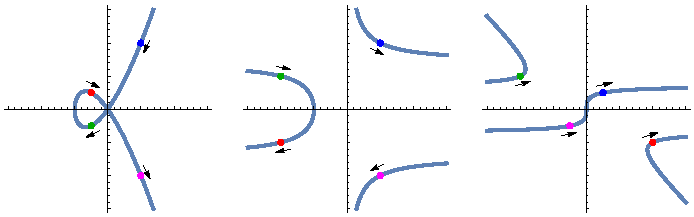
\includegraphics[width=.98\linewidth]{figures/projective-cubic-affine-charts.pdf}\par}

沿曲线仔细走一遍, 在必要时从一个仿射限制切换到另一个, 可以看出在实数域上, $X$ 构成一个\textquotedbl{}八字形\textquotedbl{}. 第一个仿射限制缺少一个点 (竖直直线上的无穷远点), 第二个和第三个各缺少两个点, 其中有一个点 (水平直线上的无穷远点) 是八字形的自交点.
\end{Example}

从射影簇 $X$ 到它的仿射限制, 只需将某个坐标设为 $1$. 但能否反过来操作? 也就是说, 从仿射簇 $X$ 出发, 能否找到一个射影簇 $\overline{X}$, 使 $X$ 是 $\overline{X}$ 的某个仿射限制? 答案是\textquotedbl{}能\textquotedbl{}, 相应的射影簇称为 $X$ 的\emph{射影闭包}, 这就是下一节的话题.

\BookExerciseHeading
\begin{BookExercises}
  \item\label{ex:intersection-of-two-projective-lines} $\mathbb{P}^{2}$ 中的直线是形如
  \[
    \mathcal{V}_{\mathbb{P}}(ax_{0}+bx_{1}+cx_{2})\subseteq\mathbb{P}^{2}
  \]
  的射影簇, 其中 $a,b,c\in K$ 不全为零. 本题设 $X$ 和 $Y$ 为 $\mathbb{P}^{2}$ 中两条不同的直线.
  \begin{enumerate}
    \item 证明存在一个仿射开片 $\mathbb{A}_{i}^{2}$, 使得仿射限制 $X_{i}$ 和 $Y_{i}$ 均非空.
    \item 不失一般性, 假设仿射限制 $X_{0}$ 和 $Y_{0}$ 在 $\mathbb{A}_{0}^{2}$ 中非空. 利用 $X$ 和 $Y$ 的定义方程, 描述 $\mathbb{A}^{2}$ 中的直线 $X_{0}$ 和 $Y_{0}$.
    \item 证明, 只要 $X_{0}$ 和 $Y_{0}$ 不平行, 就有 $X\cap Y=X_{0}\cap Y_{0}$.
    \item 证明, 当 $X_{0}$ 和 $Y_{0}$ 平行时, $X\cap Y$ 含有唯一的无穷远点.
  \end{enumerate}
  \item\label{ex:affine-patch-bijection-and-restriction}
  \begin{enumerate}
    \item 证明 $\mathbb{P}^{n}$ 中的仿射开片 $\mathbb{A}_{i}^{n}$ 与仿射空间 $\mathbb{A}^{n}$ 之间有自然双射.
    \item 若 $X=\mathcal{V}_{\mathbb{P}}(S)\subseteq\mathbb{P}^{n}$, 证明 (a) 中的双射将 $X\cap\mathbb{A}_{i}^{n}$ 与 $\mathcal{V}_{\mathbb{A}}(S_{i})\subseteq\mathbb{A}^{n}$ 认同, 其中
    \[
      S_{i}=\{f(x_{0},\ldots,x_{i-1},1,x_{i+1},\ldots,x_{n})\mid f\in S\}.
    \]
  \end{enumerate}
  \item\label{ex:three-affine-restrictions-of-a-parabola} 令 $X=\mathcal{V}_{\mathbb{P}}(x_{0}x_{2}-x_{1}^{2})\subseteq\mathbb{P}^{2}$.
  \begin{enumerate}
    \item 求三个仿射限制 $X_{0},X_{1},X_{2}$, 并画出它们在实数域上的图形.
    \item 考虑点 $(2,4)\in X_{0}\subseteq\mathbb{A}^{2}$. 作为 $X$ 的元素, 它是点 $[1:2:4]$, 这个点也属于 $X_{1}$. 这个点在 $X_{1}\subseteq\mathbb{A}^{2}$ 中的坐标是什么?
    \item 对 $X_{0}\cap X_{1}$ 中其他若干点重复 (b) 的推理, 以图示方式说明 $X_{0}$ 与 $X_{1}$ 如何在 $X$ 内拼合. 然后对 $X_{1}$ 与 $X_{2}$, 以及 $X_{0}$ 与 $X_{2}$ 也做同样的事.
  \end{enumerate}
  \item\label{ex:three-affine-restrictions-of-a-chosen-curve} 取 $X=\mathcal{V}(f)\subseteq\mathbb{P}^{2}$, 其中 $f\in K[x_{0},x_{1},x_{2}]$ 是你选取的一个齐次多项式, 重做上一题.
  \item\label{ex:affine-restrictions-of-real-projective-quadric} 画出 $X=\mathcal{V}(w^{2}+x^{2}+y^{2}-z^{2})\subseteq\mathbb{P}_{\mathbb{R}}^{3}$ 的四个仿射限制, 并描述它们如何拼合.
  \item\label{ex:affine-restrictions-of-real-split-projective-quadric} 画出 $X=\mathcal{V}(w^{2}+x^{2}-y^{2}-z^{2})\subseteq\mathbb{P}_{\mathbb{R}}^{3}$ 的四个仿射限制, 并描述它们如何拼合.
\end{BookExercises}

\section{射影闭包}\label{sec:projective-closures}

上一节把射影簇看成一个仿射簇与一组无穷远点的不交并. 本节反过来, 描述怎样向仿射簇添加无穷远点得到射影簇. 令 $j_{0}:\mathbb{A}^{n}\to\mathbb{P}^{n}$ 为函数
\[
  j_{0}(a_{1},\ldots,a_{n})=[1:a_{1}:\cdots:a_{n}],
\]
它是从 $\mathbb{A}^{n}$ 到仿射开片 $\mathbb{A}_{0}^{n}\subseteq\mathbb{P}^{n}$ 的双射. 若 $X\subseteq\mathbb{A}^{n}$ 为仿射簇, 则按构造, $j_{0}(X)\subseteq\mathbb{P}^{n}$ 是 $\mathbb{P}^{n}$ 中第一个仿射限制为 $X$ 的子集, 但 $j_{0}(X)$ 一般不是射影簇. 为了把 $j_{0}(X)$ 扩充成射影簇, 必须再添加一些点. 由此得到的最小射影簇称为 $X$ 的射影闭包.

\begin{Definition}{射影闭包}\leavevmode\label{def:projective-closure}
设 $X\subseteq\mathbb{A}^{n}$ 为仿射簇, $j_{0}(X)$ 为 $X$ 在第一个仿射开片 $\mathbb{A}_{0}^{n}\subseteq\mathbb{P}^{n}$ 中的像. $X$ 的\emph{射影闭包}, 记为 $\overline{X}\subseteq\mathbb{P}^{n}$, 是所有包含 $j_{0}(X)$ 的射影簇的交.
\end{Definition}

由于射影簇的交 (即使是无穷多个射影簇的交) 仍然是射影簇 (Exercise~\ref{ex:projective-varieties-closed-under-unions-and-intersections}), $\overline{X}$ 本身就是射影簇. 按定义, $\overline{X}$ 包含于每个包含 $j_{0}(X)$ 的射影簇, 所以可以把它看成包含 $j_{0}(X)$ 的最小射影簇.

\begin{Example}{直线的射影闭包}\leavevmode\label{ex:projective-closure-of-affine-line}
若 $X=\mathcal{V}_{\mathbb{A}}(1+x_{1}-x_{2})=\{(a,1+a)\mid a\in K\}\subseteq\mathbb{A}^{2}$, 则
\[
  j_{0}(X)=\{[1:a:1+a]\mid a\in K\}\subseteq\mathbb{P}^{2}.
\]
特别地, 当 $a\neq0$ 时,
\[
  [1:a:1+a]=[\tfrac{1}{a}:1:\tfrac{1}{a}+1],
\]
所以 $j_{0}(X)$ 包含所有形如 $[b:1:b+1]$ 且 $b\in K\setminus\{0\}$ 的点. 但包含所有这些点的射影簇也必须包含 $b=0$ 时的点 (Exercise~\ref{ex:line-limit-point-belongs-to-projective-variety}). 关键是, $K[x_{0},x_{1},x_{2}]$ 中任一多项式, 如果在所有 $b\in K\setminus\{0\}$ 对应的 $(b,1,b+1)$ 上取值为零, 那么它在 $(0,1,1)$ 上也必取值为零. 由于 $[0:1:1]\notin j_{0}(X)$, $j_{0}(X)$ 不可能是射影簇.

添加缺少的点 $[0:1:1]$ 得到射影簇
\[
  \mathcal{V}_{\mathbb{P}}(x_{0}+x_{1}-x_{2})=j_{0}(X)\sqcup\{[0:1:1]\},
\]
只须按第一个坐标为零或非零, 将 $\mathcal{V}_{\mathbb{P}}(x_{0}+x_{1}-x_{2})$ 的点分成两个不交的集合即可验证. $j_{0}(X)$ 本身不是射影簇, 而 $\mathcal{V}_{\mathbb{P}}(x_{0}+x_{1}-x_{2})$ 只比它多一个点, 所以 $\mathcal{V}_{\mathbb{P}}(x_{0}+x_{1}-x_{2})$ 是包含 $j_{0}(X)$ 的最小射影簇. 因此 $\overline{X}=\mathcal{V}_{\mathbb{P}}(x_{0}+x_{1}-x_{2})$.
\end{Example}

\begin{Example}{抛物线的射影闭包}\leavevmode\label{ex:projective-closure-of-affine-parabola}
考虑抛物线
\[
  X=\mathcal{V}_{\mathbb{A}}(x_{2}-x_{1}^{2})\subseteq\mathbb{A}^{2}.
\]
那么
\[
  j_{0}(X)=\{[1:a:a^{2}]\mid a\in K\}\subseteq\mathbb{P}^{2}.
\]
和上一例一样, 当 $a\neq0$ 时,
\[
  [1:a:a^{2}]=[\tfrac{1}{a^{2}}:\tfrac{1}{a}:1],
\]
所以对任意 $b\in K\setminus\{0\}$, $j_{0}(X)$ 都包含点 $[b^{2}:b:1]$. 同样, 包含所有这些点的射影簇也必须包含点 $[0:0:1]$. 由于 $j_{0}(X)$ 不含这个点, 它不可能是射影簇.

添加缺少的点得到射影簇
\[
  \mathcal{V}_{\mathbb{P}}(x_{0}x_{2}-x_{1}^{2})=j_{0}(X)\sqcup\{[0:0:1]\},
\]
从而 $\overline{X}=\mathcal{V}_{\mathbb{P}}(x_{0}x_{2}-x_{1}^{2})$.
\end{Example}

在前两个例子中, 仿射簇 $X$ 由一个非齐次多项式 $f$ 定义, 而 $\overline{X}$ 的定义多项式可由 $f$\textquotedbl{}齐次化\textquotedbl{}得到, 即把 $f$ 的每一项乘以 $x_{0}$ 的某个幂, 得到一个齐次多项式. 再举一例, 令
\[
  f(x_{1},x_{2},x_{3})=x_{1}^{2}+x_{2}+x_{1}x_{3}^{4}.
\]
次数最高的是最后一项, 它的次数为 $5$. 把每一项乘以 $x_{0}$ 的适当幂, 使其次数为 $5$, 就对 $f$ 作了齐次化. 得到的齐次多项式是
\[
  \overline{f}(x_{0},x_{1},x_{2},x_{3})=x_{0}^{3}x_{2}^{2}+x_{0}^{4}x_{2}+x_{1}x_{3}^{4}.
\]
下列定义描述这个一般过程.

\begin{Definition}{多项式的齐次化}\leavevmode\label{def:homogenization-of-polynomial}
设 $f\in K[x_{1},\ldots,x_{n}]$ 为 $d$ 次多项式. $f$ 的\emph{齐次化}定义为
\[
  \overline{f}=x_{0}^{d}\cdot f\biggl(\frac{x_{1}}{x_{0}},\ldots,\frac{x_{n}}{x_{0}}\biggr)
  \in K[x_{0},x_{1},\ldots,x_{n}].
\]
\end{Definition}

读者应自行验证 $\overline{f}$ 是 $d$ 次齐次多项式 (Exercise~\ref{ex:homogenization-is-homogeneous-of-same-degree}), 并且这个定义和前面逐项处理的过程一致. 将 $x_{0}=1$ 代入定义, 得
\begin{equation}\label{eq:dehomogenize-by-setting-first-coordinate-one}
  \overline{f}(1,x_{1},\ldots,x_{n})=f(x_{1},\ldots,x_{n})\in K[x_{1},\ldots,x_{n}].
\end{equation}

在 Examples~\ref{ex:projective-closure-of-affine-line} 和~\ref{ex:projective-closure-of-affine-parabola} 中, 有 $X=\mathcal{V}_{\mathbb{A}}(f)$ 和 $\overline{X}=\mathcal{V}_{\mathbb{P}}(\overline{f})$, 这或许使人猜想, 若 $X=\mathcal{V}_{\mathbb{A}}(f_{1},\ldots,f_{k})$, 就有 $\overline{X}=\mathcal{V}_{\mathbb{P}}(\overline{f}_{1},\ldots,\overline{f}_{k})$. 如果成立, 那当然很方便. 遗憾的是, 从 $X$ 到 $\overline{X}$ 的过程并不总这么简单, 如下例所示.

\begin{Example}{扭三次曲线}\leavevmode\label{ex:projective-twisted-cubic}
令 $X=\mathcal{V}_{\mathbb{A}}(x_{2}-x_{1}^{2},x_{3}-x_{1}^{3})$, 那么
\[
  j_{0}(X)=\{[1:a:a^{2}:a^{3}]\mid a\in K\}\subseteq\mathbb{P}^{3}.
\]
与 Examples~\ref{ex:projective-closure-of-affine-line} 和~\ref{ex:projective-closure-of-affine-parabola} 类似, 任何包含 $j_{0}(X)$ 的射影簇也必须包含点 $[0:0:0:1]$. 因此 $j_{0}(X)$ 不是射影簇. 但直接计算 (Exercise~\ref{ex:equations-for-projective-twisted-cubic}) 表明 $j_{0}(X)\sqcup\{[0:0:0:1]\}$ 是射影簇:
\[
  \overline{X}=\mathcal{V}_{\mathbb{P}}(x_{0}x_{2}-x_{1}^{2},x_{0}^{2}x_{3}-x_{1}^{3},x_{1}x_{3}-x_{2}^{2})
  =j_{0}(X)\cup\{[0:0:0:1]\}.
\]
这个射影簇称为\emph{扭三次曲线}.

$\overline{X}$ 的前两个定义多项式由 $X$ 的定义多项式齐次化得到, 但第三个也是必不可少的. 若没有它, 得到的是
\begin{equation}\label{eq:extra-projective-line-in-two-equation-cubic}
  \mathcal{V}_{\mathbb{P}}(x_{0}x_{2}-x_{1}^{2},x_{0}^{2}x_{3}-x_{1}^{3}),
\end{equation}
它包含 $j_{0}(X)$, 但还包含多余的点 $[0:0:b:c]\in\mathbb{P}^{3}$. 因此, 尽管 \eqref{eq:extra-projective-line-in-two-equation-cubic} 是包含 $j_{0}(X)$ 的射影簇, 它却不是 $\overline{X}$.
\end{Example}

Example~\ref{ex:projective-twisted-cubic} 说明, $X=\mathcal{V}_{\mathbb{A}}(f_{1},\ldots,f_{r})$ 的射影闭包一般不能只对 $f_{1},\ldots,f_{r}$ 齐次化得到. 但有一个解决办法: 不要只齐次化任意选取的一组定义多项式, 而应齐次化 $X$ 的消没理想中的每个多项式. 下列记号将很有用.

\begin{Definition}{集合的齐次化}\leavevmode\label{def:homogenization-of-set}
设 $S\subseteq K[x_{1},\ldots,x_{n}]$ 为多项式集合. $S$ 的\emph{齐次化}是集合
\[
  \overline{S}=\{\overline{f}\mid f\in S\}\subseteq K[x_{0},\ldots,x_{n}].
\]
\end{Definition}

\BookPairedNote
  {将仿射簇的消没理想中的每个多项式齐次化后, 就得到足够多的多项式来描述它的射影闭包. 下一个结果就是这一陈述.}
  {注意: 即使 $I$ 是理想, 它的齐次化 $\overline{I}$ 一般也不是理想. 你能看出原因吗?}

\begin{Proposition}{通过齐次化求射影闭包}\leavevmode\label{prop:projective-closure-by-homogenizing-vanishing-ideal}
若 $X\subseteq\mathbb{A}^{n}$ 为仿射簇, 则
\[
  \overline{X}=\mathcal{V}_{\mathbb{P}}\bigl(\overline{\mathcal{I}_{\mathbb{A}}(X)}\bigr)\subseteq\mathbb{P}^{n}.
\]
\end{Proposition}
\begin{Proof}
我们证明两个包含关系.

($\subseteq$) 若 $[1:a_{1}:\cdots:a_{n}]\in j_{0}(X)$ 且 $g\in\overline{\mathcal{I}_{\mathbb{A}}(X)}$, 则对某个 $f\in\mathcal{I}_{\mathbb{A}}(X)$, 有 $g=\overline{f}$, 因而 $g(1,a_{1},\ldots,a_{n})=f(a_{1},\ldots,a_{n})=0$. 所以 $\mathcal{V}_{\mathbb{P}}\bigl(\overline{\mathcal{I}_{\mathbb{A}}(X)}\bigr)$ 是包含 $j_{0}(X)$ 的射影簇. 由于 $\overline{X}$ 是包含 $j_{0}(X)$ 的最小射影簇, 得 $\overline{X}\subseteq\mathcal{V}_{\mathbb{P}}\bigl(\overline{\mathcal{I}_{\mathbb{A}}(X)}\bigr)$.

($\supseteq$) 先证明
\begin{equation}\label{eq:projective-ideal-inclusion-for-homogenized-affine-ideal}
  \mathcal{I}_{\mathbb{P}}(\overline{X})\subseteq
  \mathcal{I}_{\mathbb{P}}\Bigl(\mathcal{V}_{\mathbb{P}}\bigl(\overline{\mathcal{I}_{\mathbb{A}}(X)}\bigr)\Bigr).
\end{equation}
对这个包含关系的两边应用 $\mathcal{V}_{\mathbb{P}}$, 由 Proposition~\ref{prop:basic-properties-of-projective-vanishing-operators} 得
\[
  \overline{X}\supseteq\mathcal{V}_{\mathbb{P}}\bigl(\overline{\mathcal{I}_{\mathbb{A}}(X)}\bigr).
\]
为证明 \eqref{eq:projective-ideal-inclusion-for-homogenized-affine-ideal}, 令 $g\in\mathcal{I}_{\mathbb{P}}(\overline{X})$. 由于 $\mathcal{I}_{\mathbb{P}}(\overline{X})$ 是齐次理想, 因而有齐次生成元, 所以为证明 \eqref{eq:projective-ideal-inclusion-for-homogenized-affine-ideal}, 只须假设 $g$ 是齐次的.

即使 $g$ 是齐次的, 它也未必是 $K[x_{1},\ldots,x_{n}]$ 中某个元素的齐次化, 因为 $g$ 的每一项都可能含有 $x_{0}$. 不过, 若 $k\in\mathbb{N}$ 是使得对某个 $h\in K[x_{0},x_{1},\ldots,x_{n}]$ 有 $g=x_{0}^{k}h$ 的最大幂指数, 那么 $h=\overline{h_{0}}$, 其中 $h_{0}=h(1,x_{1},\ldots,x_{n})\in K[x_{1},\ldots,x_{n}]$ (Exercise~\ref{ex:recover-homogeneous-polynomial-not-divisible-by-first-coordinate}). 由于 $g$ 在 $\overline{X}\supseteq j_{0}(X)$ 上取值为零, 所以 $h_{0}$ 在 $X$ 上取值为零: 对任意 $(a_{1},\ldots,a_{n})\in X$, 有
\[
  h_{0}(a_{1},\ldots,a_{n})=h(1,a_{1},\ldots,a_{n})=g(1,a_{1},\ldots,a_{n})=0.
\]
因此 $h_{0}\in\mathcal{I}_{\mathbb{A}}(X)$, 所以 $h\in\overline{\mathcal{I}_{\mathbb{A}}(X)}$, 进而
\[
  g\in\langle\overline{\mathcal{I}_{\mathbb{A}}(X)}\rangle
    \subseteq\mathcal{I}_{\mathbb{P}}\Bigl(\mathcal{V}_{\mathbb{P}}\bigl(\overline{\mathcal{I}_{\mathbb{A}}(X)}\bigr)\Bigr),
\]
其中包含关系是 Proposition~\ref{prop:basic-properties-of-projective-vanishing-operators} 的再次应用. 这就证明了 \eqref{eq:projective-ideal-inclusion-for-homogenized-affine-ideal}, 也就证明了这个命题.
\end{Proof}

\begin{Example}{再看扭三次曲线}\leavevmode\label{ex:homogenizing-twisted-cubic-ideal}
根据 Proposition~\ref{prop:projective-closure-by-homogenizing-vanishing-ideal}, 可以进一步理解 Example~\ref{ex:projective-twisted-cubic} 中的现象. 当时为了计算
\[
  X=\mathcal{V}_{\mathbb{A}}(x_{2}-x_{1}^{2},x_{3}-x_{1}^{3})
\]
的射影闭包, 我们发现只齐次化 $X$ 的两个定义多项式是不够的. Proposition~\ref{prop:projective-closure-by-homogenizing-vanishing-ideal} 保证, 齐次化 $\mathcal{I}(X)$ 中的所有多项式后, 就能得到一组定义 $\overline{X}$ 的多项式. 在这个特定例子中, 只要添上另一个多项式 $x_{1}x_{3}-x_{2}^{2}\in\mathcal{I}(X)$ 的齐次化就足够了 (这个多项式碰巧是齐次的).
\end{Example}

由扭三次曲线的例子可见, 一般并没有
\[
  \overline{\mathcal{V}_{\mathbb{A}}(f_{1},\ldots,f_{k})}
    =\mathcal{V}_{\mathbb{P}}(\overline{f}_{1},\ldots,\overline{f}_{k}).
\]
但在 $k=1$ 的特殊情形, 零点定理蕴含, 射影闭包确实可由唯一的定义多项式齐次化得到.

\begin{Proposition}{超曲面的射影闭包}\leavevmode\label{prop:projective-closure-of-hypersurface}
若 $f\in K[x_{1},\ldots,x_{n}]$, 则 $\overline{\mathcal{V}_{\mathbb{A}}(f)}=\mathcal{V}_{\mathbb{P}}(\overline{f})$.
\end{Proposition}
\begin{Proof}
令 $X=\mathcal{V}_{\mathbb{A}}(f)$, 并令 $f=q_{1}^{k_{1}}\cdots q_{\ell}^{k_{\ell}}$ 为 $f$ 的由互异不可约因子给出的分解. 零点定理蕴含 $\mathcal{I}_{\mathbb{A}}(X)=\langle q_{1}\cdots q_{\ell}\rangle$. 因此由 Proposition~\ref{prop:projective-closure-by-homogenizing-vanishing-ideal}, 有
\[
  \overline{\mathcal{V}_{\mathbb{A}}(f)}=
  \mathcal{V}_{\mathbb{P}}\bigl(\overline{\mathcal{I}_{\mathbb{A}}(X)}\bigr)=
  \mathcal{V}_{\mathbb{P}}\bigl(\overline{\langle q_{1}\cdots q_{\ell}\rangle}\bigr).
\]
还须证明
\[
  \mathcal{V}_{\mathbb{P}}\bigl(\overline{\langle q_{1}\cdots q_{\ell}\rangle}\bigr)
  =\mathcal{V}_{\mathbb{P}}(\overline{f}).
\]
由于 $f\in\langle q_{1}\cdots q_{\ell}\rangle$, 有 $\overline{f}\in\overline{\langle q_{1}\cdots q_{\ell}\rangle}$, 所以 $\mathcal{V}_{\mathbb{P}}\bigl(\overline{\langle q_{1}\cdots q_{\ell}\rangle}\bigr)\subseteq\mathcal{V}_{\mathbb{P}}(\overline{f})$. 为证明反向包含, 设 $a\in\mathcal{V}_{\mathbb{P}}(\overline{f})$, 即 $\overline{f}(a)=0$. 利用齐次化的乘法性 (Exercise~\ref{ex:homogenization-multiplication-and-addition}), 有
\[
  \overline{f}=\overline{q}_{1}^{k_{1}}\cdots\overline{q}_{\ell}^{k_{\ell}},
\]
所以 $\overline{f}(a)=0$ 蕴含对某个 $i$, 有 $\overline{q}_{i}(a)=0$. 现在任取 $g\in\overline{\langle q_{1}\cdots q_{\ell}\rangle}$, 存在 $h\in K[x_{1},\ldots,x_{n}]$, 使得
\[
  g=\overline{h\cdot q_{1}\cdots q_{\ell}}=\overline{h}\cdot\overline{q}_{1}\cdots\overline{q}_{\ell}.
\]
由于某个 $\overline{q}_{i}(a)=0$, 得 $g(a)=0$. 又因为 $g$ 是 $\overline{\langle q_{1}\cdots q_{\ell}\rangle}$ 的任一元素, 所以 $a\in\mathcal{V}_{\mathbb{P}}\bigl(\overline{\langle q_{1}\cdots q_{\ell}\rangle}\bigr)$. 因此 $\mathcal{V}_{\mathbb{P}}(\overline{f})\subseteq\mathcal{V}_{\mathbb{P}}\bigl(\overline{\langle q_{1}\cdots q_{\ell}\rangle}\bigr)$, 证明完成.
\end{Proof}

关于射影闭包的最后一个重要结果是, 取射影闭包绝不会在仿射空间内部添加点, 只会添加无穷远点. 换句话说, 取仿射限制在某种意义上是取射影闭包的逆过程. 下一个结果精确地说明这一点.

\begin{Proposition}{$(\overline{X})_{0}=X$}\leavevmode\label{prop:affine-restriction-of-projective-closure}
若 $X\subseteq\mathbb{A}^{n}$ 为仿射簇, 则 $X$ 的射影闭包的仿射限制就是 $X$. 简写为 $(\overline{X})_{0}=X$.
\end{Proposition}
\begin{Proof}
设 $X\subseteq\mathbb{A}^{n}$ 为仿射簇, 令 $S=\overline{\mathcal{I}_{\mathbb{A}}(X)}$. 结合 Proposition~\ref{prop:projective-closure-by-homogenizing-vanishing-ideal} 与 Definition~\ref{def:affine-patches-and-restrictions}, 可知射影闭包 $\overline{X}=\mathcal{V}_{\mathbb{P}}(S)$ 的仿射限制是 $\mathcal{V}_{\mathbb{A}}(S_{0})$, 其中
\[
  \begin{aligned}
    S_{0}&=\{g(1,x_{1},\ldots,x_{n})\mid g\in\overline{\mathcal{I}_{\mathbb{A}}(X)}\}\\
         &=\{\overline{f}(1,x_{1},\ldots,x_{n})\mid f\in\mathcal{I}_{\mathbb{A}}(X)\}\\
         &=\mathcal{I}_{\mathbb{A}}(X).
  \end{aligned}
\]
因此 $\overline{X}$ 的仿射限制是 $\mathcal{V}_{\mathbb{A}}(\mathcal{I}_{\mathbb{A}}(X))=X$, 如所断言.
\end{Proof}

仿射限制和射影闭包在仿射簇与射影簇之间建立了密切的联系. 如前所见, 两种情形下的理论基本上是平行的. 因此, 读者或许会预期零点定理也有射影版本. 事实确实如此, 本章最后一节将证明它.

\BookExerciseHeading
\begin{BookExercises}
  \item\label{ex:line-limit-point-belongs-to-projective-variety} 设 $X\subseteq\mathbb{P}^{2}$ 为射影簇, 且对所有 $b\in K\setminus\{0\}$ 都包含点 $[b:1:b+1]$. 证明 $[0:1:1]\in X$.
  \item\label{ex:projective-variety-contains-parameter-zero-limit} 推广上一题. 设 $f_{0},\ldots,f_{n}\in K[x]$ 为一元多项式, 它们在 $0$ 处的取值不全为零. 设 $X\subseteq\mathbb{P}^{n}$ 为射影簇, 使得对所有 $b\in K\setminus\{0\}$, 都有
  \[
    [f_{0}(b):\cdots:f_{n}(b)]\in X.
  \]
  证明
  \[
    [f_{0}(0):\cdots:f_{n}(0)]\in X.
  \]
  \item\label{ex:projective-closure-of-affine-hyperbola} 改用 Examples~\ref{ex:projective-closure-of-affine-line} 和~\ref{ex:projective-closure-of-affine-parabola} 的论证, 证明仿射簇
  \[
    X=\mathcal{V}_{\mathbb{A}}(x_{1}x_{2}-1)\subseteq\mathbb{A}^{2}
  \]
  的射影闭包必须包含点 $[0:0:1]$ 和 $[0:1:0]$, 并推出
  \[
    \overline{X}=\mathcal{V}_{\mathbb{P}}(x_{1}x_{2}-x_{0}^{2}).
  \]
  画出 $X$ 在 $\mathbb{R}$ 上的图形. $X$ 的渐近线是什么, 它们与 $\overline{X}$ 的无穷远点有什么关系?
  \item\label{ex:equations-for-projective-twisted-cubic} 令
  \[
    X=\mathcal{V}_{\mathbb{A}}(x_{2}-x_{1}^{2},x_{3}-x_{1}^{3})\subseteq\mathbb{A}^{3}
  \]
  为仿射扭三次曲线.
  \begin{enumerate}
    \item 证明 $\overline{X}=\mathcal{V}_{\mathbb{P}}(x_{0}x_{2}-x_{1}^{2},x_{0}^{2}x_{3}-x_{1}^{3},x_{1}x_{3}-x_{2}^{2})$.
    \item 证明 $\overline{X}=\mathcal{V}_{\mathbb{P}}(x_{0}x_{2}-x_{1}^{2},x_{0}x_{3}-x_{1}x_{2},x_{1}x_{3}-x_{2}^{2})$.
  \end{enumerate}
  ((b) 中给出的描述是扭三次曲线更常见的表示. 注意, (b) 的三个方程是行向量为 $(x_{0},x_{1},x_{2})$ 和 $(x_{1},x_{2},x_{3})$ 的 $2\times3$ 矩阵的 $2\times2$ 子式.)
  \item\label{ex:homogenization-is-homogeneous-of-same-degree} 证明, 对任意 $d$ 次多项式 $f\in[x_{1},\ldots,x_{n}]$, 齐次化 $\overline{f}$ 是 $d$ 次齐次多项式.
  \item\label{ex:homogenization-multiplication-and-addition} 令 $f,g\in K[x_{1},\ldots,x_{n}]$.
  \begin{enumerate}
    \item 证明 $\overline{f\cdot g}=\overline{f}\cdot\overline{g}$.
    \item 是否有 $\overline{f+g}=\overline{f}+\overline{g}$? 给出证明或反例.
  \end{enumerate}
  \item\label{ex:recover-homogeneous-polynomial-not-divisible-by-first-coordinate} 设 $h\in K[x_{0},\ldots,x_{n}]$ 为齐次多项式, 且 $x_{0}\nmid h$. 证明 $h$ 是
  \[
    h(1,x_{1},\ldots,x_{n})\in K[x_{1},\ldots,x_{n}]
  \]
  的齐次化.
  \item\label{ex:closure-of-affine-ideal-variety-via-homogenization} 对任意理想 $I\subseteq K[x_{1},\ldots,x_{n}]$, 证明 $\overline{\mathcal{V}_{\mathbb{A}}(I)}=\mathcal{V}_{\mathbb{P}}(\overline{I})$. 提示: 用零点定理和 Proposition~\ref{prop:projective-closure-by-homogenizing-vanishing-ideal}, 只须证明
  \[
    \mathcal{V}_{\mathbb{P}}\bigl(\overline{\sqrt{I}}\bigr)=\mathcal{V}_{\mathbb{P}}(\overline{I}).
  \]
\end{BookExercises}

\section{射影零点定理}\label{sec:projective-nullstellensatz}

如何把零点定理的叙述改成适用于射影情形的形式? 最直接的推广, 大概是希望对任意理想 $I\subseteq K[x_{0},\ldots,x_{n}]$ 都有
\begin{equation}\label{eq:naive-projective-nullstellensatz}
  \mathcal{I}_{\mathbb{P}}(\mathcal{V}_{\mathbb{P}}(I))=\sqrt{I}.
\end{equation}
然而, 这并不完全正确. 首先, 由于消没理想是齐次的, 我们或许应当只考虑齐次理想. 但即使在齐次理想中, 仍有一种情形使 \eqref{eq:naive-projective-nullstellensatz} 不成立:
\[
  I=\langle x_{0},\ldots,x_{n}\rangle.
\]
具体来说, 若 $I=\langle x_{0},\ldots,x_{n}\rangle$, 则 $\mathcal{V}_{\mathbb{P}}(I)$ 由使多项式 $x_{0},\ldots,x_{n}$ 全部消没的点 $[a_{0}:\cdots:a_{n}]\in\mathbb{P}^{n}$ 组成. 这只有在每个 $a_{i}=0$ 时才可能. 由于 $\mathbb{P}^{n}$ 中没有这样的点, 可知 $\mathcal{V}_{\mathbb{P}}(I)=\varnothing$. 每个多项式都空真地在 $\varnothing$ 的每一点处消没, 因而 $\mathcal{I}_{\mathbb{P}}(\mathcal{V}_{\mathbb{P}}(I))=K[x_{0},\ldots,x_{n}]$. 另一方面, 注意 $I=\langle x_{0},\ldots,x_{n}\rangle$ 是根理想 (事实上是极大理想), 故 $\sqrt{I}=\langle x_{0},\ldots,x_{n}\rangle$. 合并上述观察, 得
\[
  \mathcal{I}_{\mathbb{P}}(\mathcal{V}_{\mathbb{P}}(I))
    =K[x_{0},\ldots,x_{n}]\ne\langle x_{0},\ldots,x_{n}\rangle=\sqrt{I},
\]
这就给出了 \eqref{eq:naive-projective-nullstellensatz} 的一个反例. 为了避开 \eqref{eq:naive-projective-nullstellensatz} 的这一麻烦的例外, 我们给理想 $I=\langle x_{0},\ldots,x_{n}\rangle$ 取一个名字, 强调我们不愿考虑它.

\begin{Definition}{无关理想}\leavevmode\label{def:projective-irrelevant-ideal}
理想 $\langle x_{0},\ldots,x_{n}\rangle\subseteq K[x_{0},\ldots,x_{n}]$ 称为\emph{无关理想}. $K[x_{0},\ldots,x_{n}]$ 中不同于无关理想的理想称为\emph{相关理想}.
\end{Definition}

在下面射影零点定理的叙述中, 第一条断言是弱零点定理在射影情形下的自然对应, 第二条断言则是强零点定理的自然对应.

\begin{Theorem}{射影零点定理}\leavevmode\label{thm:projective-nullstellensatz}
设 $I\subseteq K[x_{0},\ldots,x_{n}]$ 为齐次理想.
\begin{enumerate}[label=\arabic*.]
  \item $\mathcal{V}_{\mathbb{P}}(I)=\varnothing$ 当且仅当 $\sqrt{I}\supseteq\langle x_{0},\ldots,x_{n}\rangle$.
  \item 若 $\sqrt{I}$ 相关, 则 $\mathcal{I}_{\mathbb{P}}(\mathcal{V}_{\mathbb{P}}(I))=\sqrt{I}$.
\end{enumerate}
\end{Theorem}

幸运的是, 射影零点定理可以从它的仿射版本推出, 不必重新发展所需的代数工具. 关键是暂且搁置前两节讨论的方法, 转而利用另一种在仿射几何和射影几何之间转换的方法: 仿射锥.

为了引出仿射锥的概念, 注意齐次理想有两种用法: 既可用它定义射影簇 $\mathcal{V}_{\mathbb{P}}(I)\subseteq\mathbb{P}^{n}$, 也可用它定义仿射簇 $\mathcal{V}_{\mathbb{A}}(I)\subseteq\mathbb{A}^{n+1}$. 先来看一个例子, 以了解这两种观点之间的关系.

\begin{Example}{$\mathcal{V}_{\mathbb{P}}(I)$ 与 $\mathcal{V}_{\mathbb{A}}(I)$ 的比较}\leavevmode\label{ex:projective-circle-and-affine-cone}
取 $K=\mathbb{R}$, 令 $I=\langle-x_{0}^{2}+x_{1}^{2}+x_{2}^{2}\rangle\subseteq\mathbb{R}[x_{0},x_{1},x_{2}]$. 则
\[
  \mathcal{V}_{\mathbb{P}}(I)
  =\{[a_{0}:a_{1}:a_{2}]\in\mathbb{P}^{2}\mid-a_{0}^{2}+a_{1}^{2}+a_{2}^{2}=0\}.
\]
若 $a_{0}\ne0$, 同比例缩放三个坐标便可假设 $a_{0}=1$. 另一方面, 若 $a_{0}=0$, 定义方程变成 $a_{1}^{2}+a_{2}^{2}=0$, 从而 $a_{1}=a_{2}=0$. 因为 $\mathbb{P}^{2}$ 中不存在 $a_{0}=a_{1}=a_{2}=0$ 的点, 所以
\[
  \mathcal{V}_{\mathbb{P}}(I)=\{[1:a_{1}:a_{2}]\in\mathbb{P}^{2}\mid-1+a_{1}^{2}+a_{2}^{2}=0\},
\]
它与 $\mathbb{A}^{2}$ 中的单位圆, 即仿射簇 $\mathcal{V}_{\mathbb{A}}(-1+x_{1}^{2}+x_{2}^{2})\subseteq\mathbb{A}^{2}$, 有自然双射.

\BookPairedFigure{
若改把 $I$ 看作定义 $\mathbb{A}^{3}$ 中的仿射簇, 则 $\mathcal{V}_{\mathbb{A}}(I)$ 是右图所示以原点为顶点的圆锥. (图中 $x_{0}$ 是竖直坐标.) 在图中可看到, 我们已等同于单位圆的射影簇 $\mathcal{V}_{\mathbb{P}}(I)$, 正是 $\mathcal{V}_{\mathbb{A}}(I)$ 与平面 $x_{0}=1$ 的交. 进一步注意, $\mathcal{V}_{\mathbb{A}}(I)$ 可以看作所有经过原点且在 Corollary~\ref{prop:projective-space-affine-plus-infinity} 的双射下对应于 $\mathcal{V}_{\mathbb{P}}(I)$ 中的点的直线的并.
}{
\phantomsection\label{fig:projective-cone-and-circle}%
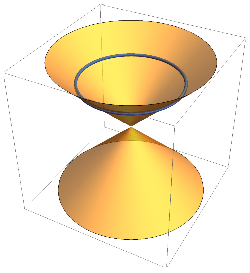
\includegraphics[width=\linewidth]{figures/projective-cone-and-circle.pdf}
}
\end{Example}

前一例中 $\mathcal{V}_{\mathbb{A}}(I)$ 是一个锥, 这并非巧合: 锥 $C\subseteq\mathbb{A}^{3}$ 具有如下性质, 只要 $(a_{0},a_{1},a_{2})\in C$, 那么整条直线
\[
  \{(\lambda a_{0},\lambda a_{1},\lambda a_{2})\mid\lambda\in K\}
\]
都包含在 $C$ 中. 从射影的观点看, 这就是说, 无论如何表示点 $[a_{0}:a_{1}:a_{2}]\in\mathbb{P}^{2}$, $[a_{0}:a_{1}:a_{2}]$ 是否属于 $C$ 都是良定义的. 有了 Example~\ref{ex:projective-circle-and-affine-cone} 的图像作为参照, 现在可以引入射影空间的子集上的仿射锥的精确定义.

\begin{Definition}{射影簇上的仿射锥}\leavevmode\label{def:affine-cone-over-projective-subset}
设 $X\subseteq\mathbb{P}^{n}$ 为一子集. $X$ 上的\emph{仿射锥}是集合
\[
  C(X)=\{(0,\ldots,0)\}\cup\{(a_{0},\ldots,a_{n})\mid[a_{0}:\cdots:a_{n}]\in X\}
  \subseteq\mathbb{A}^{n+1}.
\]
\end{Definition}

换句话说, 若 $X=\varnothing$, 则 $C(X)$ 只有原点; 否则, $C(X)$ 是与 $X\subseteq\mathbb{P}^{n}$ 中的点对应的所有过原点的直线的并. 例如, Example~\ref{ex:projective-circle-and-affine-cone} 中 $\mathcal{V}_{\mathbb{P}}(I)\subseteq\mathbb{P}^{2}$ 上的仿射锥等于 $\mathcal{V}_{\mathbb{A}}(I)\subseteq\mathbb{A}^{3}$. 这是下述引理的一个特例.

\begin{Lemma}{$\mathcal{V}_{\mathbb{A}}(I)=C(\mathcal{V}_{\mathbb{P}}(I))$}\leavevmode\label{lem:affine-vanishing-set-is-cone-of-projective-vanishing-set}
若 $I\subsetneq K[x_{0},\ldots,x_{n}]$ 为齐次理想, 则
\[
  \mathcal{V}_{\mathbb{A}}(I)=C\bigl(\mathcal{V}_{\mathbb{P}}(I)\bigr).
\]
\end{Lemma}
\begin{Proof}
首先注意, 对每个齐次理想 $I\subsetneq K[x_{0},\ldots,x_{n}]$, 有 $(0,\ldots,0)\in\mathcal{V}_{\mathbb{A}}(I)$. 为了看出这一点, 由 Proposition~\ref{prop:homogeneous-ideal-has-homogeneous-generators} 回顾, $I$ 有一组齐次生成元. 若 $(0,\ldots,0)\notin\mathcal{V}_{\mathbb{A}}(I)$, 则其中至少一个生成元必为满足 $f(0,\ldots,0)\ne0$ 的齐次多项式 $f$. 但不在 $(0,\ldots,0)$ 消没的齐次多项式只有非零常数多项式; 若 $I$ 的生成元中有这样的多项式, 则 $I=K[x_{0},\ldots,x_{n}]$, 与假设 $I\ne K[x_{0},\ldots,x_{n}]$ 矛盾.

因此, $(0,\ldots,0)\in\mathcal{V}_{\mathbb{A}}(I)$. 此外, 若 $(a_{0},\ldots,a_{n})$ 至少有一个非零坐标, 则 $I$ 的齐次性意味着
\[
  (a_{0},\ldots,a_{n})\in\mathcal{V}_{\mathbb{A}}(I)
  \iff[a_{0}:\cdots:a_{n}]\in\mathcal{V}_{\mathbb{P}}(I)
  \iff(a_{0},\ldots,a_{n})\in C(\mathcal{V}_{\mathbb{P}}(I)).
\]
这就证明了所断言的 $\mathcal{V}_{\mathbb{A}}(I)=C(\mathcal{V}_{\mathbb{P}}(I))$.
\end{Proof}

前一个引理用仿射锥联系了 $\mathcal{V}_{\mathbb{A}}$ 与 $\mathcal{V}_{\mathbb{P}}$ 算子, 下一个引理则用仿射锥联系 $\mathcal{I}_{\mathbb{A}}$ 与 $\mathcal{I}_{\mathbb{P}}$ 算子.

\begin{Lemma}{$\mathcal{I}_{\mathbb{P}}(X)=\mathcal{I}_{\mathbb{A}}(C(X))$}\leavevmode\label{lem:projective-ideal-equals-affine-ideal-of-cone}
若 $X\subseteq\mathbb{P}^{n}$ 为非空子集, 则
\[
  \mathcal{I}_{\mathbb{P}}(X)=\mathcal{I}_{\mathbb{A}}\bigl(C(X)\bigr).
\]
\end{Lemma}
\begin{Proof}
\BookPairedNote{
由于 $\mathcal{I}_{\mathbb{P}}(X)$ 是齐次理想, 它有一组齐次生成元. 由假设 $X\ne\varnothing$, 这些生成元都不可能是非零常数多项式. 因此它们全是正次数的齐次多项式, 从而在 $(0,\ldots,0)\in\mathbb{A}^{n+1}$ 处消没.
}{
Lemmas~\ref{lem:affine-vanishing-set-is-cone-of-projective-vanishing-set} 和~\ref{lem:projective-ideal-equals-affine-ideal-of-cone} 分别排除了 $I=K[x_{0},\ldots,x_{n}]$ 和 $X=\varnothing$. 这两项排除都是必要的; 见 Exercise~\ref{ex:necessity-of-affine-cone-lemma-hypotheses}.
}
所以, 对所有 $f\in\mathcal{I}_{\mathbb{P}}(X)$ 都有 $f(0,\ldots,0)=0$. 利用这一点, 可将 $\mathcal{I}_{\mathbb{P}}(X)$ 的定义重写如下:
\[
  \begin{aligned}
  \mathcal{I}_{\mathbb{P}}(X)
    &=\left\{f\in K[x_{0},\ldots,x_{n}]\ \middle|\
    \begin{gathered}
      \text{若 }[a_{0}:\cdots:a_{n}]\in X,\text{ 则 } f(a_{0},\ldots,a_{n})=0,\text{ 且}\\
      \text{若 }(a_{0},\ldots,a_{n})=(0,\ldots,0),\text{ 则 } f(a_{0},\ldots,a_{n})=0
    \end{gathered}\right\}\\
    &=\mathcal{I}_{\mathbb{A}}\bigl(\{(0,\ldots,0)\}\cup
      \{(a_{0},\ldots,a_{n})\mid[a_{0}:\cdots:a_{n}]\in X\}\bigr)\\
    &=\mathcal{I}_{\mathbb{A}}\bigl(C(X)\bigr),
  \end{aligned}
\]
如所断言.
\end{Proof}

有了 Lemmas~\ref{lem:affine-vanishing-set-is-cone-of-projective-vanishing-set} 和~\ref{lem:projective-ideal-equals-affine-ideal-of-cone}, 证明射影零点定理只需应用仿射零点定理.

\begingroup
\renewcommand{\AJProofBegin}{%
  \par\addvspace{\topsep}\noindent
  {\sffamily\bfseries\CJKfamily{pffont}Proof of Theorem~\ref{thm:projective-nullstellensatz}}\enspace\ignorespaces
}
\begin{Proof}
设 $I\subseteq K[x_{0},\ldots,x_{n}]$ 为齐次理想.

首先验证射影零点定理的第一条断言: $\sqrt{I}\supseteq\langle x_{0},\ldots,x_{n}\rangle$ 当且仅当 $\mathcal{V}_{\mathbb{P}}(I)=\varnothing$. 先假设 $\sqrt{I}\supseteq\langle x_{0},\ldots,x_{n}\rangle$. 那么
\[
  \mathcal{V}_{\mathbb{P}}(I)=\mathcal{V}_{\mathbb{P}}(\sqrt{I})
   \subseteq\mathcal{V}_{\mathbb{P}}(\langle x_{0},\ldots,x_{n}\rangle)=\varnothing,
\]
其中第一个等式就是 Exercise~\ref{ex:projective-vanishing-set-invariant-under-radical}. 反之, 假设 $\mathcal{V}_{\mathbb{P}}(I)=\varnothing$. 若 $I=K[x_{0},\ldots,x_{n}]$, 则 $\sqrt{I}=K[x_{0},\ldots,x_{n}]\supseteq\langle x_{0},\ldots,x_{n}\rangle$; 否则 $I\subsetneq K[x_{0},\ldots,x_{n}]$, 可用 Lemma~\ref{lem:affine-vanishing-set-is-cone-of-projective-vanishing-set} 得到
\[
  \mathcal{V}_{\mathbb{A}}(I)=C\bigl(\mathcal{V}_{\mathbb{P}}(I)\bigr)
    =C(\varnothing)=\{(0,\ldots,0)\},
\]
再由仿射零点定理得
\[
  \sqrt{I}=\mathcal{I}_{\mathbb{A}}(\mathcal{V}_{\mathbb{A}}(I))
  =\mathcal{I}_{\mathbb{A}}(\{(0,\ldots,0)\})=\langle x_{0},\ldots,x_{n}\rangle.
\]
两种情形都有 $\sqrt{I}\supseteq\langle x_{0},\ldots,x_{n}\rangle$, 这就证明了射影零点定理的第一部分.

为了证明射影零点定理的第二条断言, 假设 $\sqrt{I}$ 相关; 我们要证明 $\mathcal{I}_{\mathbb{P}}(\mathcal{V}_{\mathbb{P}}(I))=\sqrt{I}$. 先考虑 $\mathcal{V}_{\mathbb{P}}(I)=\varnothing$ 的情形. 由上述论证, $\sqrt{I}\supseteq\langle x_{0},\ldots,x_{n}\rangle$. 但包含 (极大的) 无关理想的相关理想只有整个环 $K[x_{0},\ldots,x_{n}]$, 故必有 $\sqrt{I}=K[x_{0},\ldots,x_{n}]$. 由于 $\mathcal{I}_{\mathbb{P}}(\mathcal{V}_{\mathbb{P}}(I))=\mathcal{I}_{\mathbb{P}}(\varnothing)=K[x_{0},\ldots,x_{n}]$, 断言 $\mathcal{I}_{\mathbb{P}}(\mathcal{V}_{\mathbb{P}}(I))=\sqrt{I}$ 在此情形下成立. 现在考虑 $\mathcal{V}_{\mathbb{P}}(I)\ne\varnothing$ 的情形. Lemma~\ref{lem:projective-ideal-equals-affine-ideal-of-cone} 给出
\[
  \mathcal{I}_{\mathbb{P}}(\mathcal{V}_{\mathbb{P}}(I))
    =\mathcal{I}_{\mathbb{A}}\bigl(C(\mathcal{V}_{\mathbb{P}}(I))\bigr).
\]
此外, 由于 $\mathcal{V}_{\mathbb{P}}(I)\ne\varnothing$, 必有 $I\subsetneq K[x_{0},\ldots,x_{n}]$, 故由 Lemma~\ref{lem:affine-vanishing-set-is-cone-of-projective-vanishing-set} 和仿射零点定理, 得
\[
  \mathcal{I}_{\mathbb{A}}\bigl(C(\mathcal{V}_{\mathbb{P}}(I))\bigr)
    =\mathcal{I}_{\mathbb{A}}(\mathcal{V}_{\mathbb{A}}(I))=\sqrt{I}.
\]
合并以上等式, 就得到了所需的 $\mathcal{I}_{\mathbb{P}}(\mathcal{V}_{\mathbb{P}}(I))=\sqrt{I}$.
\end{Proof}
\endgroup

和仿射情形一样, 射影零点定理的一个应用是显著简化射影消没理想的计算.

\begin{Example}{再看 $\mathbb{P}^{2}$ 中一条直线的消没理想}\leavevmode\label{ex:projective-line-ideal-by-nullstellensatz}
如 Example~\ref{ex:vanishing-ideal-of-projective-line-in-plane} 所示, 令 $X=\mathcal{V}_{\mathbb{P}}(x_{0}+x_{1}-x_{2})\subseteq\mathbb{P}^{2}$. 我们在 Exercise~\ref{ex:vanishing-ideal-of-projective-line-by-substitution} 中概述过直接计算 $\mathcal{I}_{\mathbb{P}}(X)$ 的方法. 有了射影零点定理, 现在只须注意 $\langle x_{0}+x_{1}-x_{2}\rangle$ 是消没集非空的齐次根理想. 因此
\[
  \mathcal{I}_{\mathbb{P}}(X)
  =\mathcal{I}_{\mathbb{P}}(\mathcal{V}_{\mathbb{P}}(\langle x_{0}+x_{1}-x_{2}\rangle))
  =\langle x_{0}+x_{1}-x_{2}\rangle.
\]
\end{Example}

与仿射情形完全相同, 射影零点定理也明确了射影 $\mathcal{V}$ 和 $\mathcal{I}$ 算子在哪些定义域上互逆. 于是可以给出射影簇与相应理想之间的下列对应表.

\begin{Proposition}{射影簇与理想}\leavevmode\label{prop:projective-variety-ideal-dictionary}
$\mathcal{V}_{\mathbb{P}}$ 和 $\mathcal{I}_{\mathbb{P}}$ 是互逆且反转包含关系的双射, 在下列理想和簇的层次之间建立对应:
\[
  \begin{array}{c@{\quad}c@{\quad}c}
  \left\{\begin{gathered}K[x_{0},\ldots,x_{n}]\text{ 中的}\\\text{相关齐次根理想}\end{gathered}\right\}
    &\longleftrightarrow&\{\mathbb{P}^{n}\text{ 中的射影簇}\}\\
  \rotatebox[origin=c]{90}{$\subseteq$} && \rotatebox[origin=c]{90}{$\subseteq$}\\
  \left\{\begin{gathered}K[x_{0},\ldots,x_{n}]\text{ 中的}\\\text{相关齐次素理想}\end{gathered}\right\}
    &\longleftrightarrow&\{\mathbb{P}^{n}\text{ 中的不可约簇}\}\\
  \rotatebox[origin=c]{90}{$\subseteq$} && \rotatebox[origin=c]{90}{$\subseteq$}\\
  \left\{\begin{gathered}K[x_{0},\ldots,x_{n}]\text{ 中的}\\\text{相关齐次极大理想}\end{gathered}\right\}
    &\longleftrightarrow&\{\mathbb{P}^{n}\text{ 中的点}\}.
  \end{array}
\]
\end{Proposition}
\begin{Proof}
设 $X\subseteq\mathbb{P}^{n}$ 为射影簇. 首先, 由 Proposition~\ref{prop:projective-vanishing-ideal-is-homogeneous-radical}, $\mathcal{I}_{\mathbb{P}}(X)$ 确实是 $K[x_{0},\ldots,x_{n}]$ 中的齐次根理想. 此外, $\mathcal{I}_{\mathbb{P}}(X)$ 不是无关理想. 为了说明这一点, 反设
\[
  \mathcal{I}_{\mathbb{P}}(X)=\langle x_{0},\ldots,x_{n}\rangle.
\]
于是 Proposition~\ref{prop:basic-properties-of-projective-vanishing-operators} 给出
\[
  X=\mathcal{V}_{\mathbb{P}}(\mathcal{I}_{\mathbb{P}}(X))
    =\mathcal{V}(\langle x_{0},\ldots,x_{n}\rangle)=\varnothing.
\]
但这样
\[
  \mathcal{I}_{\mathbb{P}}(X)=\mathcal{I}_{\mathbb{P}}(\varnothing)=K[x_{0},\ldots,x_{n}],
\]
与上述假设 $\mathcal{I}_{\mathbb{P}}(X)=\langle x_{0},\ldots,x_{n}\rangle$ 矛盾.

因此, $\mathcal{I}_{\mathbb{P}}$ 把 $\mathbb{P}^{n}$ 中任一射影簇映到 $K[x_{0},\ldots,x_{n}]$ 中的一个相关齐次根理想. 反过来, 按定义, $\mathcal{V}_{\mathbb{P}}$ 把任一这样的理想映到一个射影簇. 在这两个定义域上有
\[
  \mathcal{V}_{\mathbb{P}}(\mathcal{I}_{\mathbb{P}}(X))=X
  \qquad\text{和}\qquad
  \mathcal{I}_{\mathbb{P}}(\mathcal{V}_{\mathbb{P}}(I))=I,
\]
分别由 Proposition~\ref{prop:basic-properties-of-projective-vanishing-operators} 和射影零点定理得到. 这就证明了命题中的第一个双射. 余下两个双射由下列观察得出: $X$ 不可约当且仅当 $\mathcal{I}_{\mathbb{P}}(X)$ 为素理想 (Exercise~\ref{ex:projective-irreducibility-equivalent-to-prime-ideal}), 而 $X$ 是单个点当且仅当 $\mathcal{I}_{\mathbb{P}}(X)$ 是极大理想 (Exercise~\ref{ex:projective-single-point-equivalent-to-maximal-ideal}).
\end{Proof}

本章开始培养对射影簇的直观认识, 并以射影情形下的零点定理告一段落. 现在我们已经熟悉射影簇, 下一项任务是引入并研究它们之间保持结构的映射. 下一章将讨论这一主题.

\BookExerciseHeading
\begin{BookExercises}
  \item\label{ex:real-affine-cone-over-projective-conic} 在实数域上画出射影簇
  \[
    X=\mathcal{V}_{\mathbb{P}}(x^{2}-yz)\subseteq\mathbb{P}^{2}
  \]
  上的仿射锥. (计算机绘图软件或许有帮助.) 在图上的什么位置能看到仿射限制
  \[
    X_{0}=\mathcal{V}_{\mathbb{A}}(x^{2}-y)\subseteq\mathbb{A}^{2}?
  \]
  \item\label{ex:necessity-of-affine-cone-lemma-hypotheses}
  \begin{enumerate}
    \item 说明若 $I=K[x_{0},\ldots,x_{n}]$, Lemma~\ref{lem:affine-vanishing-set-is-cone-of-projective-vanishing-set} 不成立.
    \item 说明若 $X=\varnothing$, Lemma~\ref{lem:projective-ideal-equals-affine-ideal-of-cone} 不成立.
  \end{enumerate}
  \item\label{ex:projective-vanishing-set-invariant-under-radical} 设 $I\subseteq K[x_{0},\ldots,x_{n}]$ 为理想. 证明
  \[
    \mathcal{V}_{\mathbb{P}}(I)=\mathcal{V}_{\mathbb{P}}(\sqrt I).
  \]
  \item\label{ex:projective-vanishing-ideal-of-irreducible-polynomial} 设 $f\in K[x_{0},\ldots,x_{n}]$ 是不可约齐次多项式, 令 $X=\mathcal{V}_{\mathbb{P}}(f)\subseteq\mathbb{P}^{n}$. 证明 $\mathcal{I}_{\mathbb{P}}(X)=\langle f\rangle$.
  \item\label{ex:projective-vanishing-ideal-via-distinct-irreducible-factors} 设 $f\in K[x_{0},\ldots,x_{n}]$ 是非常数齐次多项式, 令 $X=\mathcal{V}_{\mathbb{P}}(f)\subseteq\mathbb{P}^{n}$. 用 $f$ 的互异不可约因子描述 $\mathcal{I}_{\mathbb{P}}(X)$.
  \item\label{ex:empty-projective-variety-criterion-by-degree} 证明 $\mathcal{V}_{\mathbb{P}}(f_{1},\ldots,f_{k})=\varnothing$ 当且仅当存在非负整数 $d$, 使每个 $d$ 次单项式均属于 $\langle f_{1},\ldots,f_{k}\rangle$.
\end{BookExercises}

\chapter{射影簇之间的映射}\label{chap:maps-of-projective-varieties}

\noindent\textbf{第 \thechapter{} 章学习目标}
\begin{itemize}
  \item 定义并研究射影簇之间的正则映射.
  \item 举出正则映射的各种例子, 包括线性映射, 多项式映射, 同构, 射影等价和 Veronese 嵌入.
  \item 定义 Segre 映射, 并用它们定义射影簇的积.
  \item 抽象地描述 Grassmann 簇, 并通过 Plücker 映射将它们实现为射影簇.
\end{itemize}

在第~\ref{chap:polynomial-maps}~章的引言中, 我们鼓励读者每逢引入一类新的数学对象, 就问一个关键问题: 这些对象之间哪些映射保持所关心的结构? 对于仿射簇, 最终得到适当的保结构映射概念是多项式映射. 本章的第一个目标是在射影情形中定义相应的概念.

仿射簇和射影簇之间若干关键的差别使这一目标变得复杂. 首先, 由于 $\mathbb{P}^{m}$ 定义中的等价关系, 一个多项式 $f\in K[x_{0},\ldots,x_{m}]$ 并不给出射影簇 $X\subseteq\mathbb{P}^{m}$ 上的良定义函数, 原因仅仅是多项式的值会随 $\mathbb{P}^{m}$ 中齐次坐标的缩放而改变. 不过, 若 $f$ 恰是 $d$ 次齐次多项式, 我们已经看到, 缩放齐次坐标对 $f$ 的值有一个相当简单的影响:
\[
  f(\lambda a_{0},\ldots,\lambda a_{m})=\lambda^{d}f(a_{0},\ldots,a_{m})
  \qquad\text{对所有 }\lambda\in K\setminus\{0\}.
\]
因此, 给定同为一个次数的齐次多项式 $f_{0},\ldots,f_{n}\in K[x_{0},\ldots,x_{m}]$, 其中至少有一个不在 $a$ 消没, 就得到良定义的值 $[f_{0}(a):\cdots:f_{n}(a)]\in\mathbb{P}^{n}$, 它不依赖于 $a$ 的齐次坐标的选取. 受这个观察启发, 我们以这样的多项式组为基础研究射影簇之间的映射.

一般来说, 若 $X\subseteq\mathbb{P}^{m}$ 和 $Y\subseteq\mathbb{P}^{n}$ 为射影簇, 则称函数 $F:X\to Y$ 为\emph{正则映射}, 如果它至少局部可以由一组同次数的齐次多项式 $f_{0},\ldots,f_{n}$ 实现. 正则映射是射影簇之间的保结构映射, 本章前半部分的首要目标是熟悉它们.

本章后半部分描述两种重要构造: 射影簇的积和 Grassmann 簇. 起初, 这两种构造都并不显然给出射影簇; 但对于每一种, 我们都会展示能赋予它射影簇结构的自然映射 (分别是 Segre 映射和 Plücker 映射).

\par\smallskip
{\footnotesize
\noindent\textcopyright{} The Author(s) 2025\par
\noindent E. Clader, D. Ross, \emph{Beginning in Algebraic Geometry}, Undergraduate Texts in Mathematics,
\href{https://doi.org/10.1007/978-3-031-88819-9_11}{\nolinkurl{https://doi.org/10.1007/978-3-031-88819-9_11}}.\par}

\section{射影簇之间的正则映射}\label{sec:regular-maps-of-projective-varieties}

本节的目标是熟悉两个射影簇之间正则映射的精确概念. 如本章引言中所提到的, 射影簇之间的正则映射局部以一组同次数的齐次多项式为模型. 在给出关键定义前, 先作几点观察.

设 $f\in K[x_{0},\ldots,x_{m}]$ 且 $a\in\mathbb{P}^{m}$. 选取齐次坐标并写成 $a=[a_{0}:\cdots:a_{m}]$ 后, 可以对 $f$ 求值得到
\[
  f(a_{0},\ldots,a_{m})\in K.
\]
然而, 正如我们已经看到的, 选取 $a$ 的不同齐次坐标会使对 $f$ 求值得到不同的值, 因此 $f$ 在 $\mathbb{P}^{m}$ 的点处的值不是良定义的. 为了绕开这一问题, 不妨假设 $f_{0},\ldots,f_{n}\in K[x_{0},\ldots,x_{m}]$ 都是 $d$ 次齐次多项式, 且至少一个不在 $a$ 消没. 这样可以把各个值放在一起, 把它们视为射影空间中的一个点:
\[
  [f_{0}(a_{0},\ldots,a_{m}):\cdots:f_{n}(a_{0},\ldots,a_{m})]\in\mathbb{P}^{n}.
\]
这样做带来了一个很好的结果: $\mathbb{P}^{n}$ 中的相应点实际上与 $a$ 的齐次坐标的选取无关. 的确, 若选取任意另一组齐次坐标 $a=[\lambda a_{0}:\cdots:\lambda a_{m}]$, 则
\[
  \begin{aligned}
  &[f_{0}(\lambda a_{0},\ldots,\lambda a_{m}):\cdots:f_{n}(\lambda a_{0},\ldots,\lambda a_{m})]\\
  &\qquad=[\lambda^{d}f_{0}(a_{0},\ldots,a_{m}):\cdots:\lambda^{d}f_{n}(a_{0},\ldots,a_{m})]\\
  &\qquad=[f_{0}(a_{0},\ldots,a_{m}):\cdots:f_{n}(a_{0},\ldots,a_{m})],
  \end{aligned}
\]
其中第一个等式利用各 $f_{i}$ 的齐次性, 第二个等式利用 $\mathbb{P}^{n}$ 中的等价关系. 在这种情形下, 此后采用简写
\[
  [f_{0}(a):\cdots:f_{n}(a)]=[f_{0}(a_{0},\ldots,a_{m}):\cdots:f_{n}(a_{0},\ldots,a_{m})],
\]
由于单个值 $f_{i}(a)$ 并非良定义, 这里略微滥用了记号. 在 $\mathbb{P}^{m}$ 中所有至少一个 $f_{i}$ 不消没的点处求值, 便得到函数
\[
  [f_{0}:\cdots:f_{n}]:\mathbb{P}^{m}\setminus\mathcal{V}(f_{0},\ldots,f_{n})\to\mathbb{P}^{n}.
\]
这样得到的函数自然引出射影簇之间的多项式映射概念. 这是我们在本节稍后引入的更一般的正则映射概念的初步形式.

\begin{Definition}{射影簇之间的多项式映射}\leavevmode\label{def:polynomial-maps-between-projective-varieties}
设 $X\subseteq\mathbb{P}^{m}$ 和 $Y\subseteq\mathbb{P}^{n}$ 为射影簇. 如果存在同次数的齐次多项式 $f_{0},\ldots,f_{n}\in K[x_{0},\ldots,x_{m}]$, 使得 $X\cap\mathcal{V}(f_{0},\ldots,f_{n})=\varnothing$ 且
\[
  F(a)=[f_{0}(a):\cdots:f_{n}(a)]\qquad\text{对所有 }a\in X,
\]
就称映射 $F:X\to Y$ 为\emph{多项式映射}. 若 $f_{0},\ldots,f_{n}$ 可以取为线性的, 就称 $F$ 为\emph{线性映射}.
\end{Definition}

所要求的两个条件, 即 $f_{0},\ldots,f_{n}$ 同次数且齐次, 以及 $X\cap\mathcal{V}(f_{0},\ldots,f_{n})=\varnothing$, 一起保证对每个 $a\in X$, $[f_{0}(a):\cdots:f_{n}(a)]$ 是 $\mathbb{P}^{n}$ 中良定义的点. 下面看几个具体例子.

\begin{Example}{从 $\mathbb{P}^{1}$ 到一条二次曲线的多项式映射}\leavevmode\label{ex:polynomial-map-from-projective-line-to-conic}
令 $X=\mathcal{V}(y^{2}-xz)\subseteq\mathbb{P}^{2}$, 考察函数
\[
  \begin{aligned}
    G:\mathbb{P}^{1}&\to X\\
    [a:b]&\mapsto[a^{2}:ab:b^{2}].
  \end{aligned}
\]
这是一个多项式映射: 用定义域的坐标 $s,t$ 表示, $G=[s^{2}:st:t^{2}]$. 由
\[
  \mathcal{V}(s^{2},st,t^{2})=\varnothing\subseteq\mathbb{P}^{1}
\]
可知 $G$ 在 $\mathbb{P}^{1}$ 的每一点都有定义. 为了验证 $G$ 的像落在 $X$ 内, 注意对任意 $[a:b]\in\mathbb{P}^{1}$, $X$ 的定义方程 $y^{2}-xz$ 在 $[a^{2}:ab:b^{2}]$ 处取值为零.
\end{Example}

\begin{Example}{从二次曲面到 $\mathbb{P}^{2}$ 的线性映射}\leavevmode\label{ex:linear-map-from-projective-quadric}
令 $X=\mathcal{V}(w^{2}+x^{2}+y^{2}-z^{2})\subseteq\mathbb{P}^{3}$. 由于 $[0:0:0:1]\notin X$, 得到线性映射
\[
  \begin{aligned}
    H:X&\to\mathbb{P}^{2}\\
    [a:b:c:d]&\mapsto[a:b:c],
  \end{aligned}
\]
它由齐次线性多项式 $w,x,y\in K[w,x,y,z]$ 给出.

\BookPairedFigure{
为了直观理解 $H$, 考察 $X$ 在 $w\ne0$ 的仿射开片 $\mathbb{A}^{3}_{0}$ 上的限制:
\[
  X_{0}=\mathcal{V}(1+x^{2}+y^{2}-z^{2})\subseteq\mathbb{A}^{3}.
\]
限制在这个开片时, 映射 $H$ 把 $(b,c,d)\in X_{0}$ 送到 $(b,c)\in\mathbb{A}^{2}$. 在实数域上, 可以直观地把它看成把右图中的双叶双曲面竖直投影到水平坐标平面上的二对一映射.
}{
\phantomsection\label{fig:projective-quadric-linear-projection}%
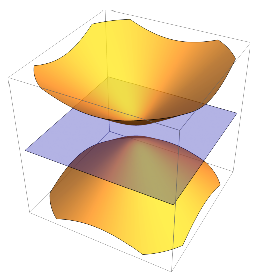
\includegraphics[width=\linewidth]{figures/projective-quadric-linear-projection.pdf}
}
\end{Example}

\begin{Example}{线性投影}\leavevmode\label{ex:linear-projections-of-projective-varieties}
推广前一例, 设 $X\subseteq\mathbb{P}^{n}$ 是不包含点 $[0:\cdots:0:1]$ 的射影簇. $X$ 到 $\mathbb{P}^{n-1}$ 的\emph{线性投影}是线性映射
\[
  \begin{aligned}
    H:X&\to\mathbb{P}^{n-1}\\
    [a_{0}:\cdots:a_{n-1}:a_{n}]&\mapsto[a_{0}:\cdots:a_{n-1}].
  \end{aligned}
\]
可以这样直观理解 $H$: 给定点 $a=[a_{0}:\cdots:a_{n}]\in X$, 存在唯一一条经过 $[0:\cdots:0:1]$ 和 $a$ 的直线 $L_{a}\subseteq\mathbb{P}^{n}$:
\[
  L_{a}=\{[ca_{0}:\cdots:ca_{n-1}:da_{n}]\mid[c:d]\in\mathbb{P}^{1}\}.
\]
这条直线与超平面 $\mathcal{V}(x_{n})\subseteq\mathbb{P}^{n}$ 相交于点 $[a_{0}:\cdots:a_{n-1}:0]$. 将 $\mathcal{V}(x_{n})$ 与 $\mathbb{P}^{n-1}$ 自然等同, 这个交点就是 $H(a)$. 因此, 可以直观地把 $H(X)$ 看作从 $[0:\cdots 0:1]$ 照来的光在 $\mathcal{V}(x_{n})$ 上投下的 $X$ 的影子. 在 $x_{0}\ne0$ 的仿射开片上, 直线 $L_{a}$ 是仅有最后一个坐标变化的\textquotedbl{}竖直\textquotedbl{}直线, 超平面 $\mathcal{V}(x_{n})$ 则是最后一个坐标为零的\textquotedbl{}水平\textquotedbl{}超平面. 因此, 如 Example~\ref{ex:linear-map-from-projective-quadric} 所示, 在这一开片内线性投影就是竖直投影.
\end{Example}

为了引出更一般的正则映射的定义, 注意 Definition~\ref{def:polynomial-maps-between-projective-varieties} 中 $X\cap\mathcal{V}(f_{0},\ldots,f_{n})=\varnothing$ 的限制常常过强. 允许映射只在\textquotedbl{}局部\textquotedbl{}用多项式描述, 会为我们提供有用的灵活性. 为了更好地理解这一点, 来看一个例子.

\begin{Example}{从二次曲线到 $\mathbb{P}^{1}$ 的分片多项式函数}\leavevmode\label{ex:piecewise-polynomial-map-from-conic}
令 $X=\mathcal{V}(y^{2}-xz)\subseteq\mathbb{P}^{2}$, 考察一对齐次线性多项式 $x,y\in K[x,y,z]$. 注意这些多项式并不给出从 $X$ 到 $\mathbb{P}^{1}$ 的多项式映射, 原因仅仅是 $\mathcal{V}(x,y)\cap X=\{[0:0:1]\}\ne\varnothing$. 不过, 我们仍得到从 $X$ 的一个子集到 $\mathbb{P}^{1}$ 的函数:
\[
  \begin{aligned}
    [x:y]:X\setminus\mathcal{V}(x,y)&\to\mathbb{P}^{1}\\
    [a:b:c]&\mapsto[a:b].
  \end{aligned}
\]
重要的是, 我们关心的不是多项式对 $(x,y)$, 而是这对多项式定义的函数 $[x:y]$. 例如, 函数 $[5x:5y]$ 与 $[x:y]$ 相同, 只因为缩放坐标不会改变 $\mathbb{P}^{1}$ 中的点. 更一般地, 回顾 $\mathbb{P}^{1}$ 中两点 $[a:b]$ 和 $[a':b']$ 相等当且仅当它们的交叉乘积 $ab'$ 和 $ba'$ 相等 (Exercise~\ref{ex:cross-multiplied-projective-coordinates}). 于是, $X$ 上的两个函数 $[f:g]$ 和 $[f':g']$ 在它们都有定义的每一点相等, 当且仅当它们的交叉乘积在 $X$ 上相等:
\[
  fg'-gf'\in\mathcal{I}(X).
\]
例如, 映射 $[x:y]$ 和 $[y:z]$ 在 $X$ 内共同定义域的每一点相等, 因为它们的交叉乘积之差是 $xz-y^{2}$, 它在 $X$ 上消没. 那么, 考察第二个函数:
\[
  \begin{aligned}
    [y:z]:X\setminus\mathcal{V}(y,z)&\to\mathbb{P}^{1}\\
    [a:b:c]&\mapsto[b:c].
  \end{aligned}
\]
注意 $[x:y]$ 和 $[y:z]$ 的定义域合起来覆盖整个 $X$, 因为第一个定义域只漏掉 $[0:0:1]$, 而第二个只漏掉 $[1:0:0]$. 由于这两个映射在它们都有定义的每一点相等, 就可以把它们合起来, 得到整个 $X$ 上分片定义的函数:
\[
  \begin{aligned}
    F:X&\to\mathbb{P}^{1}\\
    [a:b:c]&\mapsto
    \begin{cases}
      [a:b] & \text{若 }[a:b:c]\notin\mathcal{V}(x,y),\\
      [b:c] & \text{若 }[a:b:c]\notin\mathcal{V}(y,z).
    \end{cases}
  \end{aligned}
\]
\end{Example}

前例中的函数 $F:X\to\mathbb{P}^{1}$ 不能由单独一对多项式描述, 但它在以下意义上是\textquotedbl{}局部\textquotedbl{}多项式的: 对每个点 $p\in X$, 都存在一对 $f,g\in K[x,y,z]$, 不同的点可能对应不同的多项式对, 使得 $p\notin\mathcal{V}(f,g)$ 且
\[
  F(a)=[f(a):g(a)]\qquad\text{对所有 }a\in X\setminus\mathcal{V}(f,g).
\]
$F$ 的这一刻画引出了正则映射的定义.

\begin{Definition}{射影簇之间的正则映射}\leavevmode\label{def:regular-maps-between-projective-varieties}
设 $X\subseteq\mathbb{P}^{m}$ 和 $Y\subseteq\mathbb{P}^{n}$ 为射影簇. 如果对每个 $p\in X$, 均存在同次数的齐次多项式 $f_{0},\ldots,f_{n}\in K[x_{0},\ldots,x_{m}]$, 使得 $p\notin\mathcal{V}(f_{0},\ldots,f_{n})$ 且
\[
  F(a)=[f_{0}(a):\cdots:f_{n}(a)]
  \qquad\text{对所有 }a\in X\setminus\mathcal{V}(f_{0},\ldots,f_{n}),
\]
就称映射 $F:X\to Y$ 为\emph{正则映射}.
\end{Definition}

换句话说, 若对每个 $p\in X$ 都可以为 $F$ 找到一个在 $p$ 处良定义的多项式表达式, 即使这个表达式可能不在整个 $X$ 上良定义, $F:X\to Y$ 也是正则的. 由定义可知, 每个多项式映射都是正则的, 但反过来不成立: 并非每个正则映射都能在整体上用单独一组多项式描述. 下一个例子验证这一事实.

\begin{Example}{不是多项式映射的正则映射}\leavevmode\label{ex:regular-map-not-polynomial-map}
令 $X=\mathcal{V}(y^{2}-xz)\subseteq\mathbb{P}^{2}$, 再次考察 Example~\ref{ex:piecewise-polynomial-map-from-conic} 的正则映射:
\[
  \begin{aligned}
    F:X&\to\mathbb{P}^{1}\\
    [a:b:c]&\mapsto
    \begin{cases}
      [a:b] & [a:b:c]\notin\mathcal{V}(x,y),\\
      [b:c] & [a:b:c]\notin\mathcal{V}(y,z).
    \end{cases}
  \end{aligned}
\]
我们断言 $F$ 不是多项式映射. 为了说明这一点, 反设存在同为 $d$ 次的齐次多项式 $f,g\in K[x,y,z]$, 使 $\mathcal{V}(f,g)\cap X=\varnothing$ 且 $F=[f:g]$. 用 Example~\ref{ex:polynomial-map-from-projective-line-to-conic} 中的映射 $G$ 与 $F$ 复合 (先作用 $G$), 得到映射 $F\circ G:\mathbb{P}^{1}\to\mathbb{P}^{1}$. 一方面, 容易验证 $F\circ G$ 是 $\mathbb{P}^{1}$ 上的恒等映射 (见下一节的 Example~\ref{ex:projective-line-isomorphic-to-conic}); 另一方面, $F\circ G$ 也可以用 $f$ 和 $g$ 显式写成
\[
  (F\circ G)([a:b])=F([a^{2}:ab:b^{2}])=[f(a^{2},ab,b^{2}):g(a^{2},ab,b^{2})].
\]
因此, 若定义 $f_{0}(s,t)=f(s^{2},st,t^{2})$ 及 $g_{0}(s,t)=g(s^{2},st,t^{2})$, 则 $f_{0}$ 和 $g_{0}$ 都是 $K[s,t]$ 中 $2d$ 次的齐次多项式, 并定义了与恒等映射相同的多项式映射 $[f_{0}:g_{0}]:\mathbb{P}^{1}\to\mathbb{P}^{1}$. 然而, 这就产生了矛盾, 因为任何定义了 $\mathbb{P}^{1}$ 上恒等映射的多项式映射都必须具有 $f_{0}=as$ 和 $g_{0}=at$ 的形式, 其中 $a\in K$ 非零 (Exercise~\ref{ex:polynomial-representatives-of-projective-identity}). 特别地, $f_{0}$ 和 $g_{0}$ 必须是线性的, 故它们不可能对任何 $d$ 有次数 $2d$. 这一矛盾意味着 $F$ 不是多项式映射, 如所断言.
\end{Example}

最后指出, 描述正则映射的一般方法是分片定义它, 正如在 Example~\ref{ex:piecewise-polynomial-map-from-conic} 中所做的那样. 更准确地说, 射影簇 $X\subseteq\mathbb{P}^{m}$ 和 $Y\subseteq\mathbb{P}^{n}$ 之间的正则映射 $F:X\to Y$, 按定义总能用一族如下形式的函数描述:
\[
  [f_{0}:\cdots:f_{n}]:X\setminus\mathcal{V}(f_{0},\ldots,f_{n})\to Y.
\]
这族函数必须满足以下两个性质:
\begin{enumerate}[label=\arabic*.]
  \item 若 $[f_{0}:\cdots:f_{n}]$ 和 $[g_{0}:\cdots:g_{n}]$ 都在该族中, 则
  \[
    f_{i}g_{j}-f_{j}g_{i}\in\mathcal{I}(X)\qquad\text{对所有 }i,j.
  \]
  \item 每个 $p\in X$ 都必须属于该族中至少一个函数的定义域.
\end{enumerate}
第一项条件保证该族中的两个函数在共同定义域上相等, 因而可以合并它们, 得到定义域的并上的良定义函数. 第二项条件保证所有定义域的并覆盖 $X$. 事实上, 虽然从定义并不能直接看出这一点, 读者不妨验证: 每个正则映射不仅能用一族这样的函数描述, 而且能用\emph{有限}族这样的函数描述 (Exercise~\ref{ex:finite-polynomial-representations-cover-regular-map}).

\BookExerciseHeading
\begin{BookExercises}
  \item\label{ex:restrict-regular-map-to-projective-subvariety} 设 $X\subseteq\mathbb{P}^{m}$ 和 $Y\subseteq\mathbb{P}^{n}$ 为射影簇, $F:X\to Y$ 为正则映射. 若 $Z\subseteq\mathbb{P}^{m}$ 是满足 $Z\subseteq X$ 的任一射影簇, 解释为什么限制映射 $F|_{Z}:Z\to Y$ 也是正则映射.
  \item\label{ex:composition-of-projective-regular-maps} 设 $X\subseteq\mathbb{P}^{\ell}$, $Y\subseteq\mathbb{P}^{m}$, $Z\subseteq\mathbb{P}^{n}$ 均为射影簇. 若 $F:X\to Y$ 和 $G:Y\to Z$ 是正则映射, 证明 $G\circ F:X\to Z$ 也是正则的.
  \item\label{ex:regular-projection-from-projective-quadric} 令 $X=\mathcal{V}(wz-xy)\subseteq\mathbb{P}^{3}$.
  \begin{enumerate}
    \item 构造延拓函数
    \[
      [w:x]:X\setminus\mathcal{V}(w,x)\to\mathbb{P}^{1}
    \]
    的正则映射 $F:X\to\mathbb{P}^{1}$.
    \item 证明 $F$ 是满射.
    \item 对任意 $b\in\mathbb{P}^{1}$, 计算原像
    \[
      F^{-1}(b)=\{a\in X\mid F(a)=b\}.
    \]
  \end{enumerate}
  \item\label{ex:regular-map-from-projective-line-is-polynomial} 证明每个正则映射 $F:\mathbb{P}^{1}\to\mathbb{P}^{n}$ 都是多项式映射.
  \item\label{ex:coordinate-projection-does-not-extend-to-center} 证明映射
  \[
    [x_{0}:\cdots:x_{n-1}]:\mathbb{P}^{n}\setminus\mathcal{V}(x_{0},\ldots,x_{n-1})\to\mathbb{P}^{n-1}
  \]
  不能延拓为整个 $\mathbb{P}^{n}$ 上的正则映射.
  \item\label{ex:polynomial-representatives-of-projective-identity} 令 $f,g\in K[x,y]$ 为同次数的齐次多项式, 且 $\mathcal{V}(f,g)=\varnothing$, 并假设多项式映射 $[f:g]:\mathbb{P}^{1}\to\mathbb{P}^{1}$ 是恒等映射. 证明存在非零 $a\in K$, 使 $f=ax$ 且 $g=ay$.
  \item\label{ex:projective-linear-projection-is-finite-to-one} 设 $X\subseteq\mathbb{P}^{n}$ 为不包含 $[0:\cdots:0:1]$ 的射影簇, 考察线性投影
  \[
    \begin{aligned}
      H:X&\to\mathbb{P}^{n-1}\\
      [a_{0}:\cdots:a_{n-1}:a_{n}]&\mapsto[a_{0}:\cdots:a_{n-1}].
    \end{aligned}
  \]
  证明 $H$ 是有限对一的. 换句话说, 证明对任意 $b\in\mathbb{P}^{n-1}$, 原像 $H^{-1}(b)=\{a\in X\mid H(a)=b\}$ 是有限集.
  \item\label{ex:finite-polynomial-representations-cover-regular-map} 设 $X\subseteq\mathbb{P}^{m}$ 和 $Y\subseteq\mathbb{P}^{n}$ 为射影簇, $F:X\to Y$ 为正则映射. 证明存在一有限族如下形式的函数:
  \[
    [f_{0}:\cdots:f_{n}]:X\setminus\mathcal{V}(f_{0},\ldots,f_{n})\to Y,
  \]
  使得
  \begin{itemize}
    \item 该族中每个函数在自身定义域上都与 $F$ 相同, 并且
    \item $X$ 的每一点都属于该族中至少一个函数的定义域.
  \end{itemize}
\end{BookExercises}

\par\medskip
{\footnotesize
\noindent\textbf{开放获取.} 本章按照
\href{http://creativecommons.org/licenses/by-nc/4.0/}{Creative Commons Attribution-NonCommercial 4.0 International License}
的条款授权. 该许可允许以任何媒介或格式进行非商业性使用, 分享, 改编, 分发和复制, 但须对原作者和来源作适当署名, 提供 Creative Commons 许可的链接, 并说明是否作了修改.

\noindent
\begin{minipage}[t]{.17\linewidth}
  \vspace{0pt}
\includegraphics[width=.9\linewidth]{figures/source-cc-by-nc.png}
\end{minipage}\hfill
\begin{minipage}[t]{.81\linewidth}
  \vspace{0pt}本章的图片或其他第三方材料均纳入本章的 Creative Commons 许可, 除非材料的署名行另有注明. 如果材料未纳入本章的 Creative Commons 许可, 且您拟进行的使用未获法律规定的许可或超出允许使用的范围, 则须直接向著作权持有人取得许可.
\end{minipage}\par}

\section{射影簇之间的同构}\label{sec:isomorphisms-of-projective-varieties}

已经建立了适用于射影簇之间映射的概念, 现在转来讨论同构. 首先给出自然的定义.

\begin{Definition}{射影簇之间的同构}\leavevmode\label{def:isomorphism-of-projective-varieties}
射影簇 $X\subseteq\mathbb{P}^{m}$ 和 $Y\subseteq\mathbb{P}^{n}$ 之间的\emph{同构}, 是具有正则逆映射 $G:Y\to X$ 的正则映射 $F:X\to Y$. 若 $X$ 和 $Y$ 之间存在一个同构, 就称 $X$ 和 $Y$ \emph{同构}, 并记 $X\cong Y$.
\end{Definition}

\begin{BookFlowNote}{%
只要正则映射的复合仍是正则的 (已在 Exercise~\ref{ex:composition-of-projective-regular-maps} 中验证), 稍加思考便可看出, 同构是射影簇的集合上的等价关系.
}
\noindent 和仿射簇的情形一样, 我们把在同构下保持的结构看作射影簇的内在性质.

作为同构的第一个例子, 沿用上一节关于正则映射的讨论, 我们指出二次曲线 $\mathcal{V}(y^{2}-xz)\subseteq\mathbb{P}^{2}$ 与 $\mathbb{P}^{1}$ 同构.
\end{BookFlowNote}

\begin{Example}{$\mathcal{V}(y^{2}-xz)\cong\mathbb{P}^{1}$}\leavevmode\label{ex:projective-line-isomorphic-to-conic}
令 $X=\mathcal{V}(y^{2}-xz)\subseteq\mathbb{P}^{2}$, 考察分别在 Examples~\ref{ex:regular-map-not-polynomial-map} 和~\ref{ex:polynomial-map-from-projective-line-to-conic} 中引入的正则映射 $F:X\to\mathbb{P}^{1}$ 和 $G:\mathbb{P}^{1}\to X$:
\[
  F([a:b:c])=
  \begin{cases}
    [a:b] & [a:b:c]\notin\mathcal{V}(x,y),\\
    [b:c] & [a:b:c]\notin\mathcal{V}(y,z)
  \end{cases}
\]
以及
\[
  G([a:b])=[a^{2}:ab:b^{2}].
\]
现在证明这两个正则映射互逆. 给定点 $[a:b]\in\mathbb{P}^{1}$, 计算得
\[
  F(G([a:b]))=F([a^{2}:ab:b^{2}])
  =\left\{\begin{array}{ll}
    [a^{2}:ab] & \text{若 }a\ne0\\
    {[ab:b^{2}]} & \text{若 }b\ne0
  \end{array}\right\}=[a:b].
\]
反过来, 给定点 $[a:b:c]\in X$, 计算得
\[
  \begin{aligned}
  G(F([a:b:c]))
    &=G\left(\left\{\begin{array}{ll}
        [a:b] & \text{若 }(a,b)\ne(0,0)\\
        {[b:c]} & \text{若 }(b,c)\ne(0,0)
      \end{array}\right\}\right)\\
    &=\left\{\begin{array}{ll}
        [a^{2}:ab:b^{2}] & \text{若 }(a,b)\ne(0,0)\\
        {[b^{2}:bc:c^{2}]} & \text{若 }(b,c)\ne(0,0)
      \end{array}\right\}\\
    &=[a:b:c],
  \end{aligned}
\]
其中最后一个等式用到了对每个 $[a:b:c]\in X$ 都有 $b^{2}=ac$ 这一事实.

由于 $F$ 和 $G$ 是互逆的正则映射, 得到 $X\cong\mathbb{P}^{1}$.
\end{Example}

射影空间上的线性变换给出一类很特殊的同构. 为了建立记号, 设 $A$ 是元素在 $K$ 中的可逆 $(n+1)\times(n+1)$ 矩阵. 对每个点 $p\in\mathbb{P}^{n}$, 定义新点 $Ap\in\mathbb{P}^{n}$: 选取 $p$ 的齐次坐标, 将它们视为列向量, 再用矩阵 $A$ 左乘这个列向量. 例如, 如果
\[
  A=\begin{pmatrix}
     1&1&0\\
     1&0&2\\
     0&1&-1
  \end{pmatrix}
\]
且 $p=[a_{0}:a_{1}:a_{2}]$, 则 $Ap=[a_{0}+a_{1}:a_{0}+2a_{2}:a_{1}-a_{2}]$.

更一般地, 若记 $A=(A_{ij})$, 则上述过程给出线性映射 $F_{A}:\mathbb{P}^{n}\to\mathbb{P}^{n}$, 它由以 $A$ 各行为系数的线性多项式定义:
\[
  F_{A}=\left[\sum_{j=0}^{n}A_{0j}x_{j}:\cdots:\sum_{j=0}^{n}A_{nj}x_{j}\right].
\]
$A$ 的可逆性意味着 $F_{A}$ 在 $\mathbb{P}^{n}$ 的每一点都有定义, 而且 $F_{A}$ 的逆是正则映射
\[
  F_{A^{-1}}:\mathbb{P}^{n}\to\mathbb{P}^{n}
\]
(见 Exercise~\ref{ex:invertible-matrix-induces-projective-isomorphism}). 因此, $F_{A}$ 是 $\mathbb{P}^{n}$ 到自身的线性同构, 我们给这样由可逆矩阵产生的同构一个专门名称.

\begin{Definition}{射影等价}\leavevmode\label{def:projective-equivalence}
$\mathbb{P}^{n}$ 的一个\emph{射影等价}是形如
\[
  \begin{aligned}
    F_{A}:\mathbb{P}^{n}&\to\mathbb{P}^{n}\\
    p&\mapsto Ap,
  \end{aligned}
\]
的同构, 其中 $A$ 为元素在 $K$ 中的可逆 $(n+1)\times(n+1)$ 矩阵. 若存在射影等价 $F_{A}:\mathbb{P}^{n}\to\mathbb{P}^{n}$ 使得 $F_{A}(X)=Y$, 就称两个射影簇 $X,Y\subseteq\mathbb{P}^{n}$ \emph{射影等价}.
\end{Definition}

\BookPairedNote{
直观地看, 射影等价就是 $\mathbb{P}^{n}$ 中的线性坐标变换, 类似于向量空间中的换基. 若 $X,Y\subseteq\mathbb{P}^{n}$ 射影等价, 则它们同构. 的确, 若 $F_{A}:\mathbb{P}^{n}\to\mathbb{P}^{n}$ 是满足 $F_{A}(X)=Y$ 的射影等价, 则限制 $F_{A}:X\to Y$ 是具有正则逆映射 $F_{A^{-1}}:Y\to X$ 的正则映射.
}{
学过复分析的读者可能遇到过 $\mathbb{P}^{1}$ 的射影等价, 它们在复分析中称为\textquotedbl{}Möbius 变换\textquotedbl{}.
}
重要的是, $\mathbb{P}^{n}$ 的射影等价把射影簇映到射影簇. 具体地说, 若 $X\subseteq\mathbb{P}^{n}$ 是射影簇, 且 $F_{A}:\mathbb{P}^{n}\to\mathbb{P}^{n}$ 是射影等价, 则 $F_{A}(X)$ 也是 $\mathbb{P}^{n}$ 中的射影簇 (Exercise~\ref{ex:projective-equivalence-preserves-varieties}). 对任何正则映射 $F:\mathbb{P}^{m}\to\mathbb{P}^{n}$, 同一断言更一般地成立 (Theorem~\ref{thm:regular-images-of-projective-varieties-are-closed}), 但证明后一事实要困难得多.

下面来看 $\mathbb{P}^{2}$ 中射影等价的一个具体例子.

\begin{Example}{射影等价的二次曲线}\leavevmode\label{ex:projectively-equivalent-complex-conics}
考察两个复射影簇
\[
  X=\mathcal{V}(x^{2}+y^{2}+z^{2})\subseteq\mathbb{P}^{2}_{\mathbb{C}}
  \qquad\text{和}\qquad
  Y=\mathcal{V}(y^{2}-xz)\subseteq\mathbb{P}^{2}_{\mathbb{C}}.
\]
我们断言 $X$ 和 $Y$ 射影等价, 并将通过对定义方程作坐标变换来展示这一点. 更具体地说, 注意
\[
  x^{2}+y^{2}+z^{2}=y^{2}-(xi+z)(xi-z).
\]
从而 $[a:b:c]\in X$ 当且仅当 $[ai+c:b:ai-c]\in Y$. 换句话说, 令 $A$ 为可逆矩阵
\[
  A=\begin{pmatrix}
    i&0&1\\
    0&1&0\\
    i&0&-1
  \end{pmatrix},
\]
可知 $F_{A}(X)=Y$, 故 $X$ 和 $Y$ 射影等价.
\end{Example}

事实上, 前一例还可以用一种颇为意外的方式推广.

\begin{Proposition}{所有不可约二次曲线都射影等价}\leavevmode\label{prop:irreducible-conics-projectively-equivalent}
设 $f,g\in K[x,y,z]$ 为不可约的二次齐次多项式. 则 $\mathcal{V}(f)$ 和 $\mathcal{V}(g)$ 在 $\mathbb{P}^{2}$ 中射影等价.
\end{Proposition}
\begin{Proof}
要证明所有不可约二次曲线都射影等价, 只需证明它们都与一条特定的二次曲线射影等价. 更具体地说, 设 $f\in K[x,y,z]$ 为不可约的二次齐次多项式; 我们证明 $\mathcal{V}(f)$ 与 $\mathcal{V}(xy+xz+yz)$ 射影等价.

首先, 选取两个不同的点 $[a_{1}:b_{1}:c_{1}],[a_{2}:b_{2}:c_{2}]\in\mathcal{V}(f)$, 并考察矩阵
\[
  \begin{pmatrix}
    a_{1}&a_{2}\\
    b_{1}&b_{2}\\
    c_{1}&c_{2}
  \end{pmatrix}.
\]
由于两列互不为标量倍数, 这个矩阵的秩为二, 因而各行之间有一个在相差标量倍数意义下唯一的线性关系. 如果 $\mathcal{V}(f)$ 中任意选取的第三个点也满足这一线性关系, 则 $\mathcal{V}(f)$ 的所有点都在 $\mathbb{P}^{2}$ 中的一条直线上, 与 $f$ 的不可约性矛盾. 因此, 必有第三个点 $[a_{3}:b_{3}:c_{3}]\in\mathcal{V}(f)$ 不满足这个线性关系, 从而矩阵
\[
  A=\begin{pmatrix}
    a_{1}&a_{2}&a_{3}\\
    b_{1}&b_{2}&b_{3}\\
    c_{1}&c_{2}&c_{3}
  \end{pmatrix}
\]
的各行线性无关, 因而它可逆.

由矩阵 $A$ 定义的射影等价 $F_{A}$ 把三点 $[1:0:0],[0:1:0],[0:0:1]\in\mathbb{P}^{2}$ 映到我们在 $\mathcal{V}(f)$ 上选取的三个点. 因此, 逆射影等价 $F_{A^{-1}}$ 把 $\mathcal{V}(f)$ 等同于一条不可约二次曲线 $\mathcal{V}(g)\subseteq\mathbb{P}^{2}$, 使得 $[1:0:0],[0:1:0],[0:0:1]\in\mathcal{V}(g)$. 而二次齐次多项式在这三点处消没, 当且仅当它具有形式
\[
  g=\alpha xy+\beta xz+\gamma yz,
\]
其中 $\alpha,\beta,\gamma\in K$. 由 $g$ 的不可约性可知, $\alpha,\beta,\gamma$ 均非零. 于是, 射影等价 $[a:b:c]\mapsto[\gamma^{-1}a:\beta^{-1}b:\alpha^{-1}c]$ 把 $\mathcal{V}(g)$ 等同于 $\mathcal{V}(xy+xz+yz)$. 将以上射影等价复合, 可知 $\mathcal{V}(f)$ 与 $\mathcal{V}(xy+xz+yz)$ 射影等价.
\end{Proof}

\begin{Corollary}{所有不可约二次曲线都同构于 $\mathbb{P}^{1}$}\leavevmode\label{cor:irreducible-conics-isomorphic-to-projective-line}
设 $f\in K[x,y,z]$ 为不可约的二次齐次多项式. 则
\[
  \mathcal{V}(f)\cong\mathbb{P}^{1}.
\]
\end{Corollary}
\begin{Proof}
由 Proposition~\ref{prop:irreducible-conics-projectively-equivalent}, 所有不可约二次曲线都射影等价, 因而同构. 再由 Example~\ref{ex:projective-line-isomorphic-to-conic}, 不可约二次曲线 $\mathcal{V}(y^{2}-xz)$ 与 $\mathbb{P}^{1}$ 同构. 因此 $\mathbb{P}^{2}$ 中所有不可约二次曲线都同构于 $\mathbb{P}^{1}$.
\end{Proof}

Corollary~\ref{cor:irreducible-conics-isomorphic-to-projective-line} 表明, $\mathbb{P}^{2}$ 中不可约二次曲线的内在性质相当简单, 因为它们都同构于 $\mathbb{P}^{1}$. 但要提醒读者, 不要因此以为 $\mathbb{P}^{2}$ 中更高次曲线的内在性质也同样简单. 事实上, 只需把次数提高一次, 就可以证明 $\mathbb{P}^{2}$ 中的不可约三次曲线有无穷多个不同的同构类, 它们都不与 $\mathbb{P}^{1}$ 同构 (在 Example~\ref{ex:irreducible-projective-cubic-not-isomorphic-to-line} 中, 我们给出一个不与 $\mathbb{P}^{1}$ 同构的不可约三次曲线的具体例子). $\mathbb{P}^{2}$ 中的三次曲线是研究椭圆曲线的基础. 椭圆曲线是一个引人入胜的数学分支, 许多研究者将整个职业生涯投入其中, 不过本书不会涉及这一主题.

关于同构的讨论自然引出一个问题: 如何研究射影簇的内在性质? 在仿射情形下, 我们引入了仿射簇的坐标环作为这方面的关键工具: 两个仿射簇同构当且仅当它们的坐标环同构, 从而可以通过研究坐标环的代数结构来研究仿射簇的内在性质. 受仿射情形的启发, 不妨问是否存在某个代数对象, 能刻画射影簇的内在性质. 沿用仿射情形中的发展, 很自然地可以引入射影簇 $X\subseteq\mathbb{P}^{n}$ 的\emph{齐次坐标环}, 定义为商环
\[
  \frac{K[x_{0},\ldots,x_{n}]}{\mathcal{I}(X)}.
\]
遗憾的是, 与仿射情形不同, 齐次坐标环在同构下并不保持, 如下一例所示.

\begin{Example}{同构与齐次坐标环}\leavevmode\label{ex:isomorphism-does-not-preserve-homogeneous-coordinate-ring}
Example~\ref{ex:projective-line-isomorphic-to-conic} 表明 $X=\mathcal{V}(y^{2}-xz)\subseteq\mathbb{P}^{2}$ 与 $\mathbb{P}^{1}$ 同构. 不过, 这两个射影簇的齐次坐标环分别为
\[
  \frac{K[x,y,z]}{\langle y^{2}-xz\rangle}
  \qquad\text{和}\qquad K[s,t],
\]
而这两个环并不同构. 特别是, 后者是唯一分解整环, 但方程 $y^{2}=xz$ 蕴含前者不是.

也可以用另一种方式看出这两个环并不同构: 如果它们同构, 则由仿射簇情形下代数与几何的等价性, 仿射簇 $\mathcal{V}_{\mathbb{A}}(y^{2}-xz)$ 和 $\mathbb{A}^{2}$ 应当同构. 但它们并不同构: 前者在原点有一个奇点, 而后者是非奇异的.
\end{Example}

\BookPairedNoteLeft{
齐次坐标环在射影代数几何中起重要作用, 但不是本书论述的重点.
}{
尽管前一例说明齐次坐标环不是射影簇的完全代数不变量, 仍有一种可能: 每个射影簇或许还对应另一个环, 能够编码它的全部内在结构.
}
事实并非如此. 正如下一章将看到的, 射影簇的内在性质不是由单独一个环决定的, 而是由一族环决定的. 每个环记录射影簇的局部几何信息, 整体几何则由这些局部环之间的同态决定.

不过, 暂且不要走得太远. 在本章余下部分, 我们将介绍 Veronese, Segre 和 Plücker 这三族经典映射, 继续加深对射影簇之间映射的实际理解.

\BookExerciseHeading
\begin{BookExercises}
  \item\label{ex:twisted-cubic-isomorphic-to-projective-line} 令 $X=\mathcal{V}(x_{0}x_{2}-x_{1}^{2},x_{0}x_{3}-x_{1}x_{2},x_{1}x_{3}-x_{2}^{2})\subseteq\mathbb{P}^{3}$ 为扭三次曲线. 考察映射
  \[
    \begin{aligned}
      F:\mathbb{P}^{1}&\to X\\
      [a:b]&\mapsto[a^{3}:a^{2}b:ab^{2}:b^{3}].
    \end{aligned}
  \]
  通过构造正则逆映射, 证明 $F$ 是同构.
  \item\label{ex:linear-variety-of-independent-polynomials-is-projective-space} 设 $\ell_{1},\ldots,\ell_{k}\in K[x_{0},\ldots,x_{n}]$ 为线性无关的齐次线性多项式. 证明 $\mathcal{V}(\ell_{1},\ldots,\ell_{k})\cong\mathbb{P}^{n-k}$.
  \item\label{ex:invertible-matrix-induces-projective-isomorphism} 设 $A$ 是元素在 $K$ 中的可逆 $(n+1)\times(n+1)$ 矩阵.
  \begin{enumerate}
    \item 证明 $F_{A}:\mathbb{P}^{n}\to\mathbb{P}^{n}$ 是正则映射.
    \item 证明 $F_{A^{-1}}$ 是 $F_{A}$ 的逆.
  \end{enumerate}
  \item\label{ex:projective-equivalence-preserves-varieties} 设 $A$ 是元素在 $K$ 中的可逆 $(n+1)\times(n+1)$ 矩阵.
  \begin{enumerate}
    \item 令 $X=\mathcal{V}(f_{1},\ldots,f_{k})\in\mathbb{P}^{n}$. 证明
    \[
      F_{A}(X)=\mathcal{V}(f_{1}\circ A^{-1},\ldots,f_{k}\circ A^{-1}).
    \]
    (这里, 自然地把每个 $f_{i}$ 看作函数 $f_{i}:K^{n+1}\to K$, 把 $A^{-1}$ 看作函数 $A^{-1}:K^{n+1}\to K^{n+1}$.) 特别地, 若 $X$ 为射影簇, 则 $F_{A}(X)$ 也是射影簇.
    \item 设 $X,Y\subseteq\mathbb{P}^{n}$ 射影等价. 证明 $X$ 不可约当且仅当 $Y$ 不可约.
  \end{enumerate}
  \item\label{ex:projective-equivalence-preserves-homogeneous-coordinate-ring} 设 $X,Y\subseteq\mathbb{P}^{n}$ 为射影等价的两个射影簇. 证明
  \[
    \frac{K[x_{0},\ldots,x_{n}]}{\mathcal{I}(X)}
    \cong
    \frac{K[x_{0},\ldots,x_{n}]}{\mathcal{I}(Y)}.
  \]
  因此, 虽然齐次坐标环在同构下不保持, 但在射影等价下保持.
  \item\label{ex:normal-form-and-finite-fibres-of-projective-linear-map} 设 $X\subseteq\mathbb{P}^{n}$ 为射影簇, 设 $\ell_{0},\ldots,\ell_{k}\in K[x_{0},\ldots,x_{n}]$ 为齐次线性多项式, 且 $\mathcal{V}(\ell_{0},\ldots,\ell_{k})\cap X=\varnothing$. 考察线性映射
  \[
    \begin{aligned}
      L:X&\to\mathbb{P}^{k}\\
      a&\mapsto[\ell_{0}(a):\cdots:\ell_{k}(a)].
    \end{aligned}
  \]
  \begin{enumerate}
    \item 证明存在一对射影等价 $F_{A}:\mathbb{P}^{n}\to\mathbb{P}^{n}$ 和 $F_{B}:\mathbb{P}^{k}\to\mathbb{P}^{k}$, 使对所有 $a=[a_{0}:\cdots:a_{n}]\in X$, 都有
    \[
      F_{B}(L(F_{A}(a)))=[a_{0}:\cdots:a_{j}],
    \]
    其中 $j\le k$. (提示: 对以 $\ell_{1},\ldots,\ell_{k}$ 的系数为各行的 $k\times n$ 矩阵作行, 列运算, 可以将其化为形如
    \[
      \begin{pmatrix}
        I&0\\
        0&0
      \end{pmatrix}
    \]
    的矩阵, 其中 $I$ 表示某个 $j\le k$ 对应的 $j\times j$ 单位矩阵, 每个 $0$ 表示相应大小的零矩阵.)
    \item 利用 (a) 证明 $L$ 是有限对一的. (提示: 见 Exercise~\ref{ex:projective-linear-projection-is-finite-to-one}.)
  \end{enumerate}
\end{BookExercises}

\section{Veronese 映射}\label{sec:veronese-maps}

本节介绍以意大利数学家 Giuseppe Veronese (1854--1917) 命名的 Veronese 映射. 这是一族射影空间之间的正则映射, 可用固定次数的所有单项式来描述. 在实际应用中, Veronese 映射的作用在于, 它们使我们能够降低射影簇及其间映射的次数. 更确切地说, 如本节将看到的, 可以借助 Veronese 映射证明以下两个令人意外的性质.
\begin{enumerate}[label=\arabic*.]
  \item 在同构意义下, 每个射影簇都可以实现为一族次数至多为二的多项式的消没集 (Proposition~\ref{prop:projective-varieties-defined-by-quadratics}).
  \item 在同构意义下, 射影簇之间的每个多项式映射都是线性映射 (Proposition~\ref{prop:projective-polynomial-maps-linear-up-to-isomorphism}).
\end{enumerate}
现在从定义入手, 开始讨论 Veronese 映射.

\begin{Definition}{Veronese 映射}\leavevmode\label{def:veronese-map}
对任意 $d,n\ge1$, \emph{Veronese 映射} $F_{d,n}:\mathbb{P}^{n}\to\mathbb{P}^{\binom{d+n}{d}-1}$ 是多项式映射
\[
  F_{d,n}=[x_{0}^{d}:x_{0}^{d-1}x_{1}:x_{0}^{d-1}x_{2}:\cdots:x_{n}^{d}],
\]
其中出现在定义中的单项式是变量 $x_{0},\ldots,x_{n}$ 的所有 $d$ 次单项式.
\end{Definition}

Exercise~\ref{ex:count-veronese-monomials-by-stars-and-bars} 概述了一种证明方法, 说明变量 $x_{0},\ldots,x_{n}$ 的 $d$ 次单项式恰有 $\binom{d+n}{d}$ 个 (这解释了作为 $F_{d,n}$ 陪域的射影空间的维数). 此外, Exercise~\ref{ex:veronese-monomials-have-no-common-zero} 要求读者验证, 这些单项式不在 $\mathbb{P}^{n}$ 的任何一点同时消没, 从而解释 $F_{d,n}$ 的定义域为什么是整个 $\mathbb{P}^{n}$.

作为第一个例子, 取 $d=2$ 和 $n=1$, Veronese 映射为
\[
  \begin{aligned}
    F_{2,1}:\mathbb{P}^{1}&\to\mathbb{P}^{2}\\
    [a:b]&\mapsto[a^{2}:ab:b^{2}],
  \end{aligned}
\]
这就是我们在 Examples~\ref{ex:polynomial-map-from-projective-line-to-conic} 和~\ref{ex:projective-line-isomorphic-to-conic} 中考察过的映射 $G$. 在那个特例中, 我们把像 $F_{2,1}(\mathbb{P}^{1})$ 描述为射影簇 $\mathcal{V}(y^{2}-xz)\subseteq\mathbb{P}^{2}$. 下一个目标是把这一描述推广到任意 $d$ 和 $n$ 的 $F_{d,n}(\mathbb{P}^{n})$. 要把任意 Veronese 映射的像描述为射影簇, 首先为 $F_{d,n}$ 陪域的坐标建立方便的记号.

注意, 变量 $x_{0},\ldots,x_{n}$ 的 $d$ 次单项式可以用满足 $d_{0}+\cdots+d_{n}=d$ 的非负整数元组 $D=(d_{0},\ldots,d_{n})$ 来编号. 更确切地说, 与 $D=(d_{0},\ldots,d_{n})$ 对应的单项式为
\[
  x^{D}=x_{0}^{d_{0}}x_{1}^{d_{1}}\cdots x_{n}^{d_{n}}.
\]
据此, 对每个这样的元组 $D$, 将 $\mathbb{P}^{\binom{d+n}{d}-1}$ 的相应坐标记为 $y_{D}$, 从而 $F_{d,n}$ 是 $y_{D}$ 坐标为 $x^{D}$ 的多项式映射.

例如, 在前面考察的 $(d,n)=(2,1)$ 情形下, 将 $\mathbb{P}^{2}$ 的坐标记为 $y_{(2,0)}$, $y_{(1,1)}$ 和 $y_{(0,2)}$. 此时 $F_{2,1}$ 将 $a=[a_{0}:a_{1}]$ 映到 $y_{(2,0)}$ 坐标为 $a_{0}^{2}$, $y_{(1,1)}$ 坐标为 $a_{0}a_{1}$, $y_{(0,2)}$ 坐标为 $a_{1}^{2}$ 的点. 由此可见, $F_{2,1}$ 映到簇
\[
  \mathcal{V}\bigl(y_{(2,0)}y_{(0,2)}-y_{(1,1)}^{2}\bigr)\subseteq\mathbb{P}^{2}.
\]
更一般地, Veronese 映射的像由下面的结果描述.

\begin{Proposition}{Veronese 映射的像}\leavevmode\label{prop:veronese-image-defined-by-quadratics}
对任意 $d,n\ge1$, Veronese 映射 $F_{d,n}:\mathbb{P}^{n}\to\mathbb{P}^{\binom{d+n}{d}-1}$ 的像为
\[
  X_{d,n}
  =\mathcal{V}\bigl(\{y_{D}y_{D'}-y_{E}y_{E'}\mid D+D'=E+E'\}\bigr)
  \subseteq\mathbb{P}^{\binom{d+n}{d}-1}.
\]
\end{Proposition}
\begin{Proof}
$F_{d,n}(\mathbb{P}^{n})\subseteq X_{d,n}$ 来自如下观察: 对任意 $a\in\mathbb{P}^{n}$ 及满足 $D+D'=E+E'$ 的任意元组 $D,D',E,E'$, 有
\[
  a^{D}a^{D'}-a^{E}a^{E'}
  =a_{0}^{d_{0}+d_{0}'}\cdots a_{n}^{d_{n}+d_{n}'}
   -a_{0}^{e_{0}+e_{0}'}\cdots a_{n}^{e_{n}+e_{n}'}=0.
\]
反过来, 为证明 $F_{d,n}(\mathbb{P}^{n})\supseteq X_{d,n}$, 令 $b\in X_{d,n}$. 则对满足 $D+D'=E+E'$ 的所有元组 $D,D',E,E'$, $b$ 的坐标满足 $b_{D}b_{D'}=b_{E}b_{E'}$. 由这些关系可证明 (Exercise~\ref{ex:veronese-coordinate-products-depend-on-sum}) 对满足 $D_{1}+\cdots+D_{k}=E_{1}+\cdots+E_{k}$ 的所有元组 $D_{1},\ldots,D_{k},E_{1},\ldots,E_{k}$, 有
\begin{equation}\label{eq:veronese-equality-of-coordinate-products}
  b_{D_{1}}\cdots b_{D_{k}}=b_{E_{1}}\cdots b_{E_{k}}.
\end{equation}
特别是, 对 $D=(d_{0},\ldots,d_{n})$, 有
\begin{equation}\label{eq:veronese-coordinate-power-from-pure-powers}
  b_{D}^{d}=b_{(d,0,\ldots,0)}^{d_{0}}b_{(0,d,0,\ldots,0)}^{d_{1}}
  \cdots b_{(0,\ldots,0,d)}^{d_{n}}.
\end{equation}
因此坐标 $b_{(d,0,\ldots,0)},b_{(0,d,0,\ldots,0)},\ldots,b_{(0,\ldots,0,d)}$ 中至少一个非零, 否则由 \eqref{eq:veronese-coordinate-power-from-pure-powers} 可得对所有 $D$ 都有 $b_{D}=0$, 这在射影空间中是不可能的.

于是, 不妨设 $b_{(d,0,\ldots,0)}$ 非零, 从而可缩放 $b$ 的齐次坐标, 使 $b_{(d,0,\ldots,0)}=1$. 对每个 $1\le i\le n$, 定义
\[
  a_{i}=b_{(d-1,0,\ldots,0,1,0,\ldots,0)},
\]
其中 $1$ 出现在下标元组的第 $i$ 个坐标. 我们断言
\begin{equation}\label{eq:veronese-preimage-coordinate-reconstruction}
  F_{d,n}(a)=b.
\end{equation}
为证明 \eqref{eq:veronese-preimage-coordinate-reconstruction}, 注意 $F_{d,n}$ 和 $a_{i}$ 的定义意味着, 对任意 $D=(d_{0},\ldots,d_{n})$, $F_{d,n}(a)$ 的 $y_{D}$ 坐标为
\[
  \begin{aligned}
  a_{0}^{d_{0}}a_{1}^{d_{1}}\cdots a_{n}^{d_{n}}
    &=b_{(d,0,\ldots,0)}^{d_{0}}b_{(d-1,1,0,\ldots,0)}^{d_{1}}
      \cdots b_{(d-1,0,\ldots,0,1)}^{d_{n}}\\
    &=b_{(d,0,\ldots,0)}^{d-1}b_{D}=b_{D},
  \end{aligned}
\]
其中第二个等式是 \eqref{eq:veronese-equality-of-coordinate-products} 的应用, 第三个等式来自 $b_{(d,0,\ldots,0)}=1$. 这就证明了断言 \eqref{eq:veronese-preimage-coordinate-reconstruction}, 从而完成了 $X_{d,n}=F_{d,n}(\mathbb{P}^{n})$ 的证明.
\end{Proof}

Proposition~\ref{prop:veronese-image-defined-by-quadratics} 推广了 Example~\ref{ex:projective-line-isomorphic-to-conic} 的一个方面: 它给出了 $F_{d,n}$ 所映入的簇的显式定义方程. 但在 Example~\ref{ex:projective-line-isomorphic-to-conic} 中, 我们实际上还证明了更多: Veronese 映射 $F_{2,1}$ 是到其像上的同构. 这一事实对所有 Veronese 映射也成立.

\begin{Proposition}{Veronese 映射是嵌入}\leavevmode\label{prop:veronese-maps-are-embeddings}
对任意 $d,n\ge1$, Veronese 映射 $F_{d,n}:\mathbb{P}^{n}\to X_{d,n}$ 是同构.
\end{Proposition}
\begin{Proof}
\BookPairedNote{
为证明 $F_{d,n}$ 是到 $X_{d,n}$ 上的同构, 我们构造正则逆映射 $G_{d,n}:X_{d,n}\to\mathbb{P}^{n}$. 给定任意 $b\in X_{d,n}$, 用如下分片描述定义 $G_{d,n}(b)$:
}{
在许多数学语境下,\textquotedbl{}嵌入\textquotedbl{}指到其像上的同构.
}
\[
  G_{d,n}(b)=\left\{\begin{array}{l}
  [b_{(d,0,\ldots,0)}:b_{(d-1,1,\ldots,0)}:\cdots:b_{(d-1,0,\ldots,1)}]\\
  {[b_{(1,d-1,\ldots,0)}:b_{(0,d,\ldots,0)}:\cdots:b_{(0,d-1,\ldots,1)}]}\\
  \multicolumn{1}{c}{\vdots}\\
  {[b_{(1,0,\ldots,d-1)}:b_{(0,1,\ldots,d-1)}:\cdots:b_{(0,0,\ldots,d)}]}
  \end{array}\right.,
\]
各表达式在它给出 $\mathbb{P}^{n}$ 中良定义的点的所有位置都适用. 由 $X_{d,n}$ 的定义方程可见, $G_{d,n}$ 的任意两个表达式的交叉乘积 (见 Exercise~\ref{ex:cross-multiplied-projective-coordinates}) 在 $X_{d,n}$ 上相等, 因此 $G_{d,n}$ 在其有定义的每一点均为良定义. 此外, 如 Proposition~\ref{prop:veronese-image-defined-by-quadratics} 的证明所示, 对每个 $b\in X_{d,n}$, 坐标 $b_{(d,0,\ldots,0)},b_{(0,d,\ldots,0)},\ldots,b_{(0,0,\ldots,d)}$ 中至少一个非零, 从而 $G_{d,n}$ 在所有 $b\in X_{d,n}$ 上都有定义. 因此 $G_{d,n}:X_{d,n}\to\mathbb{P}^{n}$ 是正则映射. 还需核对 $F_{d,n}$ 与 $G_{d,n}$ 是互逆函数, 这留给读者作为习题 (Exercise~\ref{ex:veronese-piecewise-inverse}).
\end{Proof}

簇 $X_{d,n}\subseteq\mathbb{P}^{\binom{n+d}{d}}$ 称为 \emph{Veronese 簇}. Proposition~\ref{prop:veronese-maps-are-embeddings} 表明, 在同构意义下, Veronese 簇 $X_{d,n}$ 就其内在性质而言, 不过是从另一角度看待射影空间 $\mathbb{P}^{n}$. 但研究 $\mathbb{P}^{n}$ 的各种 Veronese 模型, 可以降低射影簇 $X\subseteq\mathbb{P}^{n}$ 的定义多项式的最高次数. 在介绍这一过程一般如何进行之前, 先看一个具体例子.

\begin{Example}{一条三次曲线的 Veronese 像}\leavevmode\label{ex:veronese-image-of-projective-cubic-curve}
令 $X=\mathcal{V}(x_{0}^{3}+x_{1}^{3}+x_{2}^{3})\subseteq\mathbb{P}^{2}$, 考察 Veronese 映射
\[
  F_{3,2}:X\to\mathbb{P}^{\binom{5}{3}-1}=\mathbb{P}^{9}.
\]
回顾 $\mathbb{P}^{9}$ 的坐标 $y_{D}$ 由满足 $d_{0}+d_{1}+d_{2}=3$ 的三元组 $D=(d_{0},d_{1},d_{2})$ 编号. 注意对任意 $a=[a_{0}:a_{1}:a_{2}]\in\mathbb{P}^{2}$, 有
\[
  a\in X\iff a_{0}^{3}+a_{1}^{3}+a_{2}^{3}=0
  \iff F_{3,2}(a)\in\mathcal{V}(y_{(3,0,0)}+y_{(0,3,0)}+y_{(0,0,3)}).
\]
由此得
\[
  F_{3,2}(X)=X_{3,2}\cap\mathcal{V}\bigl(y_{(3,0,0)}+y_{(0,3,0)}+y_{(0,0,3)}\bigr).
\]
此外, 由 Proposition~\ref{prop:veronese-maps-are-embeddings}, $F_{3,2}$ 给出同构 $\mathbb{P}^{2}\cong X_{3,2}$, 从而 $F_{3,2}$ 的限制给出同构
\[
  X\cong X_{3,2}\cap\mathcal{V}\bigl(y_{(3,0,0)}+y_{(0,3,0)}+y_{(0,0,3)}\bigr).
\]
由于 Proposition~\ref{prop:veronese-image-defined-by-quadratics} 表明 $X_{3,2}$ 由二次多项式定义, 这意味着 $X$ 同构于一个可以用次数至多为二的多项式定义的射影簇, 尽管 $X$ 原来的表达式把它描述为一个三次多项式的消没集.
\end{Example}

在前例基础上, 现在描述一般结果.

\begin{Proposition}{射影簇由二次多项式定义}\leavevmode\label{prop:projective-varieties-defined-by-quadratics}
在同构意义下, 每个射影簇都可以写成一族有限个次数至多为二的齐次多项式的消没集.
\end{Proposition}
\begin{Proof}
令 $X\subseteq\mathbb{P}^{n}$ 为射影簇. 首先注意 (Exercise~\ref{ex:choose-projective-defining-polynomials-of-common-degree}), 可以写 $X=\mathcal{V}(f_{1},\ldots,f_{k})$, 其中每个 $f_{i}\in K[x_{0},\ldots,x_{n}]$ 都是同为 $d$ 次的齐次多项式. 换句话说, 可以把每个 $f_{i}$ 写成
\[
  f_{i}=\sum_{D}a_{i,D}x_{0}^{d_{0}}\cdots x_{n}^{d_{n}},
\]
其中求和遍历所有元素之和为 $d$ 的非负整数元组 $D=(d_{0},\ldots,d_{n})$, 且 $a_{i,D}\in K$. 考察 Veronese 映射
\[
  F_{d,n}:\mathbb{P}^{n}\to\mathbb{P}^{\binom{n+d}{d}-1},
\]
用陪域的变量定义线性多项式 $\ell_{1},\ldots,\ell_{k}$:
\[
  \ell_{i}=\sum_{D}a_{i,D}y_{D}.
\]
如 Example~\ref{ex:veronese-image-of-projective-cubic-curve} 所示, 对任意 $a\in\mathbb{P}^{n}$, 有
\[
  a\in X\iff F_{d,n}(a)\in X_{d,n}\cap\mathcal{V}(\ell_{1},\ldots,\ell_{k}),
\]
从而 $F_{d,n}(X)=X_{d,n}\cap\mathcal{V}(\ell_{1},\ldots,\ell_{k})$. 由于 $F_{d,n}:\mathbb{P}^{n}\to\mathbb{P}^{\binom{n+d}{d}-1}$ 是正则映射, 它可限制为正则映射
\[
  F_{d,n}:X\to X_{d,n}\cap\mathcal{V}(\ell_{1},\ldots,\ell_{k}).
\]
又因为 $F_{d,n}$ 是到 $X_{d,n}$ 上的同构 (Proposition~\ref{prop:veronese-maps-are-embeddings}), 所以 $F_{d,n}^{-1}:X_{d,n}\to\mathbb{P}^{n}$ 可限制为正则逆映射
\[
  F_{d,n}^{-1}:X_{d,n}\cap\mathcal{V}(\ell_{1},\ldots,\ell_{k})\to X.
\]
因此, $X\cong X_{d,n}\cap\mathcal{V}(\ell_{1},\ldots,\ell_{k})$. 由 $X_{d,n}$ 可以用二次多项式定义 (Proposition~\ref{prop:veronese-image-defined-by-quadratics}), 而各 $\ell_{i}$ 都是线性的, 结论随即成立.
\end{Proof}

值得注意的是, Proposition~\ref{prop:projective-varieties-defined-by-quadratics} 虽然降低了射影簇的定义多项式的最高次数, 却通常会使定义多项式的数量大幅增加. 例如, 在 Example~\ref{ex:veronese-image-of-projective-cubic-curve} 中, 可以利用维数理论基本定理的一个射影版本 (将在本书最后一章中精确说明), 证明描述这条三次曲线的 Veronese 像至少需要 8 个线性和二次多项式, 虽然三次曲线本身只需一个定义多项式.

作为 Veronese 映射的最后一个应用, 下一个结果说明, 在对定义域作同构的意义下, 所有多项式映射都是线性映射.

\begin{Proposition}{在同构意义下, 多项式映射是线性的}\leavevmode\label{prop:projective-polynomial-maps-linear-up-to-isomorphism}
若 $F:X\to Y$ 是射影簇之间的多项式映射, 则存在同构 $G:X\to Z$ 及线性映射 $L:Z\to Y$, 使 $F=L\circ G$.
\end{Proposition}
\begin{Proof}
Exercise~\ref{ex:linearize-projective-polynomial-map-by-veronese}.
\end{Proof}

Proposition~\ref{prop:projective-polynomial-maps-linear-up-to-isomorphism} 的一个令人意外的推论, 是下述关于多项式映射的有限对一结果. 这再次表明多项式映射的限制有多强, 也进一步说明我们一直研究的较灵活的正则映射概念为何合理: 正则映射只在局部是多项式的.

\begin{Corollary}{多项式映射是有限对一的}\leavevmode\label{cor:projective-polynomial-maps-are-finite-to-one}
若 $F:X\to Y$ 是射影簇之间的多项式映射, 则对任意 $b\in Y$, 使 $F(a)=b$ 的 $a\in X$ 只有有限个.
\end{Corollary}
\begin{Proof}
沿用 Proposition~\ref{prop:projective-polynomial-maps-linear-up-to-isomorphism} 陈述中的记号, 任意多项式映射 $F$ 都可写成复合 $L\circ G$, 其中 $G$ 是同构, $L$ 是线性的. 由同构是一对一的, 而射影簇之间的线性映射是有限对一的 (Exercise~\ref{ex:normal-form-and-finite-fibres-of-projective-linear-map}), 即得结论.
\end{Proof}

Exercise~\ref{ex:regular-projection-from-projective-quadric} 给出了一个不是有限对一的正则映射的例子. 于是, 由 Corollary~\ref{cor:projective-polynomial-maps-are-finite-to-one}, 这个正则映射不是多项式映射.

\BookExerciseHeading
\begin{BookExercises}
  \item\label{ex:count-veronese-monomials-by-stars-and-bars} 设 $d,n\ge1$ 为整数, 令 $SB_{d,n}$ 为由 $d$ 个\textquotedbl{}星号\textquotedbl{}和 $n$ 个\textquotedbl{}竖线\textquotedbl{}组成的序列的集合. 例如, 当 $(d,n)=(4,3)$ 时, $SB_{d,n}$ 的几个元素为
  \[
    (\star\mid\star\star\mid\mid\star),\qquad
    (\mid\mid\mid\star\star\star\star),\qquad
    (\star\mid\star\mid\star\mid\star).
  \]
  \begin{enumerate}
    \item 解释为什么 $SB_{d,n}$ 有 $\binom{d+n}{d}$ 个元素.
    \item 描述 $SB_{d,n}$ 和变量 $x_{0},\ldots,x_{n}$ 的 $d$ 次单项式的集合之间的双射.
    \item 由 (a) 和 (b) 推出变量 $x_{0},\ldots,x_{n}$ 的 $d$ 次单项式恰有 $\binom{d+n}{d}$ 个.
  \end{enumerate}
  \item\label{ex:veronese-monomials-have-no-common-zero} 证明第 $d$ 个 Veronese 映射 $F_{d,n}$ 在 $\mathbb{P}^{n}$ 的每一点都正则.
  \item\label{ex:veronese-coordinate-products-depend-on-sum} 令 $X_{d,n}\subseteq\mathbb{P}^{\binom{d+n}{d}-1}$ 为 Veronese 簇, 考察一点 $b\in X_{d,n}$. 本题证明坐标的乘积
  \[
    b_{D_{1}}\cdots b_{D_{k}}\in K
  \]
  只依赖于 $D_{1}+\cdots+D_{k}\in\mathbb{N}^{n+1}$. 固定一个满足 $e_{0}+\cdots+e_{n}=dk$ 的元组 $(e_{0},\ldots,e_{n})\in\mathbb{N}^{n+1}$. 令 $\mathcal{S}$ 表示长度为 $dk$ 的序列的集合, 其中有 $e_{0}$ 个元素等于 $0$, 有 $e_{1}$ 个元素等于 $1$, 依此类推. 对每个 $\sigma\in\mathcal{S}$, 令
  \[
    b_{\sigma}=b_{D_{1}}\cdots b_{D_{k}},
  \]
  以定义 $b_{\sigma}\in K$, 其中 $D_{j}$ 的第 $i$ 项为 $\sigma$ 的第 $j$ 个长度为 $d$ 的子序列中 $i$ 的个数.
  \begin{enumerate}
    \item 为理解记号, 考察元组 $(e_{0},e_{1},e_{2})=(3,2,4)$, 这里取 $n=2$ 和 $d=k=3$. 写出三个序列 $\sigma\in\mathcal{S}$ 的例子及相应的值 $b_{\sigma}\in K$.
    \item 证明将 $\sigma$ 送到 $b_{\sigma}$ 的函数 $\phi:\mathcal{S}\to K$ 满射到
    \[
      \{b_{D_{1}}\cdots b_{D_{k}}\mid D_{1}+\cdots+D_{k}=(e_{1},\ldots,e_{n})\}.
    \]
    \item 设 $\sigma$ 与 $\sigma'$ 是 $\mathcal{S}$ 中仅相差两个元素对换的序列. 用 $X_{d,n}$ 的定义方程证明
    \[
      \phi(\sigma)=\phi(\sigma').
    \]
    \item 用对换生成所有排列这一事实, 推出 $b_{D_{1}}\cdots b_{D_{k}}$ 只依赖于 $D_{1}+\cdots+D_{k}$.
  \end{enumerate}
  \item\label{ex:veronese-piecewise-inverse} 沿用 Proposition~\ref{prop:veronese-maps-are-embeddings} 证明中的记号, 验证 $F_{d,n}$ 和 $G_{d,n}$ 是互逆函数.
  \item\label{ex:choose-projective-defining-polynomials-of-common-degree}
  \begin{enumerate}
    \item 令 $f\in K[x_{0},\ldots,x_{n}]$ 且 $d\in\mathbb{N}$. 证明
    \[
      \mathcal{V}_{\mathbb{P}}(f)=\mathcal{V}_{\mathbb{P}}(x_{0}^{d}f,\ldots,x_{n}^{d}f).
    \]
    \item 证明每个射影簇都可以用一组有限个同次数的齐次多项式定义.
  \end{enumerate}
  \item\label{ex:linearize-projective-polynomial-map-by-veronese} 证明 Proposition~\ref{prop:projective-polynomial-maps-linear-up-to-isomorphism}. (提示: 取 $G$ 为一个 Veronese 映射.)
\end{BookExercises}

\section{积与 Segre 映射}\label{sec:products-and-segre-maps}

本节的首要目标是研究射影簇的积. 射影情形下积的概念要比仿射情形复杂不少. 复杂性来自这样一个事实: 在仿射情形有自然等同 $\mathbb{A}^{m}\times\mathbb{A}^{n}=\mathbb{A}^{m+n}$, 但 $\mathbb{P}^{m}\times\mathbb{P}^{n}$ 与 $\mathbb{P}^{m+n}$ 之间没有这样的等同, 建议读者思考其中的原因. 事实上, 起初甚至并不清楚怎样把 $\mathbb{P}^{m}\times\mathbb{P}^{n}$ 本身解释为射影簇. 第一项任务是把 $\mathbb{P}^{m}\times\mathbb{P}^{n}$ 单射到一个更大的射影空间中, 从而将其解释为射影簇. 为此使用 Segre 映射, 它们以意大利数学家 Corrado Segre (1863--1924) 命名.

\begin{Definition}{Segre 映射}\leavevmode\label{def:segre-map}
对任意 $m,n\ge0$, 从 $\mathbb{P}^{m}\times\mathbb{P}^{n}$ 到 $\mathbb{P}^{(m+1)(n+1)-1}$ 的 \emph{Segre 映射} $S_{m,n}$ 由下式给出:
\[
  S_{m,n}=[x_{0}y_{0}:x_{0}y_{1}:\cdots:x_{m}y_{n-1}:x_{m}y_{n}],
\]
其中定义中的单项式是所有可能的乘积 $x_{i}y_{j}$.
\end{Definition}

为了理解这个定义, 我们先看第一个有意思的例子.

\begin{Example}{Segre 映射 $S_{1,1}$}\leavevmode\label{ex:segre-product-of-two-projective-lines}
考察 $m=n=1$ 时的 Segre 映射:
\[
  \begin{aligned}
    S_{1,1}:\mathbb{P}^{1}\times\mathbb{P}^{1}&\to\mathbb{P}^{3}\\
    ([a_{0}:a_{1}],[b_{0}:b_{1}])&\mapsto[a_{0}b_{0}:a_{0}b_{1}:a_{1}b_{0}:a_{1}b_{1}].
  \end{aligned}
\]
注意, 缩放任一个 $\mathbb{P}^{1}$ 中的齐次坐标只会使像中的所有坐标作相同的缩放. 此外, 可以验证
\[
  a_{0}b_{0}=a_{0}b_{1}=a_{1}b_{0}=a_{1}b_{1}=0
  \implies a_{0}=a_{1}=0\quad\text{或}\quad b_{0}=b_{1}=0.
\]
这两个观察合起来意味着, $S_{1,1}$ 在 $\mathbb{P}^{1}\times\mathbb{P}^{1}$ 的每一点均为良定义. 建议读者推广这一点, 验证 $S_{m,n}$ 在 $\mathbb{P}^{m}\times\mathbb{P}^{n}$ 的每一点均为良定义 (Exercise~\ref{ex:segre-map-well-defined}).
\end{Example}

尽管 Segre 映射在定义域的每一点均为良定义, 此时问它们是不是正则映射还没有意义, 原因只在于尚未赋予定义域射影簇结构. 事实上, 我们恰要利用 Segre 映射, 赋予 $\mathbb{P}^{m}\times\mathbb{P}^{n}$ 在 $\mathbb{P}^{(m+1)(n+1)-1}$ 中的射影簇结构. 为此, 引入一种能方便地组织 $\mathbb{P}^{(m+1)(n+1)-1}$ 的坐标的记号.

注意 $\mathbb{P}^{(m+1)(n+1)-1}$ 有 $(m+1)(n+1)$ 个齐次坐标; 将这些坐标记为 $z_{ij}$, 其中 $0\le i\le m$ 且 $0\le j\le n$. 方便的是, 可以自然地把这些坐标排成一个 $m\times n$ 矩阵 $A(z)$, 其第 $ij$ 项为 $z_{ij}$. 按这样的标记, 约定 Segre 映射 $S_{m,n}$ 的 $z_{ij}$ 坐标为 $x_{i}y_{j}$. 现在用这个记号描述 Segre 映射的像.

\begin{Proposition}{Segre 映射单射到一个射影簇上}\leavevmode\label{prop:segre-map-injective-with-determinantal-image}
对任意 $m,n\ge0$, Segre 映射 $S_{m,n}$ 是 $\mathbb{P}^{m}\times\mathbb{P}^{n}$ 到射影簇 $Z_{m,n}\subseteq\mathbb{P}^{(m+1)(n+1)-1}$ 上的单射, 其中
\[
  Z_{m,n}=\mathcal{V}\bigl(\{z_{ij}z_{k\ell}-z_{i\ell}z_{kj}
      \mid 0\le i,k\le m,\ 0\le j,\ell\le n\}\bigr).
\]
\end{Proposition}
\begin{Proof}
\BookPairedNote{
我们证明 $S_{m,n}$ 的像等于 $Z_{m,n}$, 而把 $S_{m,n}$ 是单射的验证留作习题 (Exercise~\ref{ex:segre-map-injective}).
}{
$Z_{m,n}$ 由矩阵 $A(z)$ 的所有 $2\times2$ 子式定义, 因此是\textquotedbl{}行列式簇\textquotedbl{}的一个例子.
}
为证明 $S_{m,n}$ 的像包含在 $Z_{m,n}$ 中, 只须证明 $z_{ij}z_{k\ell}-z_{i\ell}z_{kj}$ 在 $S_{m,n}$ 像中的任一点消没. 这来自对任意 $(a,b)\in\mathbb{P}^{m}\times\mathbb{P}^{n}$, 都有
\[
  (a_{i}b_{j})(a_{k}b_{\ell})-(a_{i}b_{\ell})(a_{k}b_{j})=0.
\]
反过来, 为证明 $Z_{m,n}$ 包含在 $S_{m,n}$ 的像中, 令 $c\in Z_{m,n}$. 这意味着 $A(c)$ 的所有 $2\times2$ 子式都消没, 从而 $A(c)$ 的秩至多为一; 换句话说, $A(c)$ 的每一行都是某一行的倍数. 由于必有至少一行非零, 不妨设首行非零, 并将其记为 $b=(b_{0},\ldots,b_{n})$. 令 $a_{i}\in K$ 为使 $A(c)$ 的第 $i$ 行等于 $a_{i}b$ 的值. 容易验证
\[
  c=S_{m,n}([1:a_{1}:\cdots:a_{m}],[b_{0}:b_{1}:\cdots:b_{n}]),
\]
所以 $c$ 在 $S_{m,n}$ 的像中.
\end{Proof}

\begin{Example}{$S_{1,1}$ 的像}\leavevmode\label{ex:segre-image-of-two-projective-lines}
再考察 $m=n=1$ 的情形, 把 $\mathbb{P}^{3}$ 的坐标记为 $z_{00},z_{01},z_{10},z_{11}$. Proposition~\ref{prop:segre-map-injective-with-determinantal-image} 表明, $S_{1,1}$ 是到 $\mathbb{P}^{3}$ 中由以下 $2\times2$ 行列式的消没定义的射影簇上的单射:
\[
  \det\begin{pmatrix}
    z_{00}&z_{01}\\
    z_{10}&z_{11}
  \end{pmatrix}=z_{00}z_{11}-z_{01}z_{10}.
\]
\end{Example}

Proposition~\ref{prop:segre-map-injective-with-determinantal-image} 的重要性在于, 它将积 $\mathbb{P}^{m}\times\mathbb{P}^{n}$ 与 $\mathbb{P}^{(m+1)(n+1)-1}$ 中的一个射影簇等同, 从而给出了将积本身视为射影簇的一种自然方式. 下一个结果表明, 可以用 Segre 映射自然地把任意两个射影簇的积视为射影簇, 不限于射影空间的积.

\begin{Proposition}{射影簇的积}\leavevmode\label{prop:segre-map-restricts-to-product-of-projective-varieties}
若 $X\subseteq\mathbb{P}^{m}$ 和 $Y\subseteq\mathbb{P}^{n}$ 为射影簇, 则 Segre 映射 $S_{m,n}$ 限制为从 $X\times Y$ 到 $\mathbb{P}^{(m+1)(n+1)-1}$ 中的一个射影簇上的单射.
\end{Proposition}
\begin{Proof}
设 $X=\mathcal{V}(\mathcal{S})$ 且 $Y=\mathcal{V}(\mathcal{T})$, 其中 $\mathcal{S}\subseteq K[x_{0},\ldots,x_{m}]$ 且 $\mathcal{T}\subseteq K[y_{0},\ldots,y_{n}]$. 对每个 $f\in\mathcal{S}$ 和 $g\in\mathcal{T}$, 以及每个 $0\le i\le n$ 和 $0\le j\le m$, 定义
\[
  f_{i}=f(z_{0i},z_{1i},\ldots,z_{mi})
  \qquad\text{和}\qquad
  g_{j}=g(z_{j0},z_{j1},\ldots,z_{jn}).
\]
令 $\mathcal{S}'$ 为所有这类 $f_{i}$ 的集合, $\mathcal{T}'$ 为所有这类 $g_{j}$ 的集合. 建议读者验证 (Exercise~\ref{ex:equations-for-segre-image-of-product})
\[
  S_{m,n}(X\times Y)=S_{m,n}(\mathbb{P}^{m}\times\mathbb{P}^{n})
  \cap\mathcal{V}(\mathcal{S}'\cup\mathcal{T}').
\]
由 Proposition~\ref{prop:segre-map-injective-with-determinantal-image} 可知, $S_{m,n}$ 是单射, 且 $S_{m,n}(\mathbb{P}^{m}\times\mathbb{P}^{n})$ 是射影簇. 由于射影簇的交本身也是射影簇, 我们得出 $S_{m,n}(X\times Y)$ 是射影簇.
\end{Proof}

现在用 Segre 映射把 $X\times Y$ 与射影簇 $S_{m,n}(X\times Y)$ 等同, 从而在射影簇的范畴内定义积.

\begin{Definition}{射影簇的积}\leavevmode\label{def:product-of-projective-varieties}
若 $X\subseteq\mathbb{P}^{m}$ 和 $Y\subseteq\mathbb{P}^{n}$ 为射影簇, 则它们的\emph{积} $X\times Y$ (作为射影簇) 定义为射影簇
\[
  S_{m,n}(X\times Y)\subseteq\mathbb{P}^{(m+1)(n+1)-1}.
\]
\end{Definition}

\begin{Example}{一张双直纹曲面}\leavevmode\label{ex:segre-quadric-is-doubly-ruled}
我们停下来直观地看一下射影簇 $\mathbb{P}^{1}\times\mathbb{P}^{1}$. 由 Definition~\ref{def:product-of-projective-varieties} 和 Example~\ref{ex:segre-image-of-two-projective-lines}, 它等于射影簇 $\mathcal{V}(z_{00}z_{11}-z_{01}z_{10})\subseteq\mathbb{P}^{3}$.

\BookPairedFigure{
考察 $z_{00}\ne0$ 的仿射限制, 它是仿射曲面
\[
  \mathcal{V}_{\mathbb{A}}(z_{11}-z_{01}z_{10})\subseteq\mathbb{A}^{3}.
\]
右图描绘的是这一仿射限制在 $\mathbb{R}$ 上的情形. 可以看出这张曲面是双直纹的: 有两种不同的方式将它看作直线的不交并.
}{
\phantomsection\label{fig:segre-doubly-ruled-surface}%
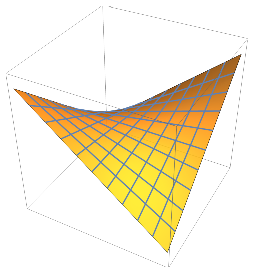
\includegraphics[width=\linewidth]{figures/segre-doubly-ruled-surface.pdf}
}
这一仿射限制的双直纹反映了一个更一般的事实: 射影曲面 $\mathbb{P}^{1}\times\mathbb{P}^{1}\subseteq\mathbb{P}^{3}$ 也是双直纹的, 有两种不同的方式将它实现为 $\mathbb{P}^{3}$ 中 (射影) 直线的不交并. $\mathbb{P}^{1}\times\mathbb{P}^{1}$ 的两族直纹由 $\mathbb{P}^{3}$ 中形如
\[
  \{a\}\times\mathbb{P}^{1}\qquad\text{和}\qquad\mathbb{P}^{1}\times\{b\}
\]
的子集给出, 建议读者在 Exercise~\ref{ex:two-rulings-of-segre-quadric} 中探究这一点.
\end{Example}

把积 $X\times Y$ 实现为射影簇后, 就可以讨论从 $X\times Y$ 出发和到 $X\times Y$ 的正则映射. 下面的结果涉及从积出发的正则映射中最重要的两个例子: 两个投影映射.

\begin{Proposition}{投影映射是正则的}\leavevmode\label{prop:product-projections-are-regular}
若 $X\subseteq\mathbb{P}^{m}$ 和 $Y\subseteq\mathbb{P}^{n}$ 为射影簇, 则投影映射 $\pi_{1}:X\times Y\to X$ 和 $\pi_{2}:X\times Y\to Y$ 都是正则的.
\end{Proposition}
\begin{Proof}
只考虑 $\pi_{1}$; $\pi_{2}$ 的论证可由对称性得到. 只需注意, 对任意 $c=(a,b)\in X\times Y\subseteq\mathbb{P}^{(m+1)(n+1)-1}$, 可以用如下分片表达式写出 $\pi_{1}(c)$:
\[
  \pi_{1}(c)=\begin{cases}
    [c_{00}:c_{10}:\cdots:c_{m0}] & c\notin\mathcal{V}(z_{00},z_{10},\ldots,z_{m0})\\
    \vdots & \vdots\\
    [c_{0n}:c_{1n}:\cdots:c_{mn}] & c\notin\mathcal{V}(z_{0n},z_{1n},\ldots,z_{mn}).
  \end{cases}
\]
为验证上述 $\pi_{1}$ 的表达式, 设 $c=(a,b)\in X\times Y$. 则 $c$ 的 $z_{ij}$ 坐标为 $a_{i}b_{j}$. 注意, $a$ 至少有一个非零坐标, $b$ 也至少有一个非零坐标. 若 $b_{j}\ne0$, 则 $c\notin\mathcal{V}(z_{0j},z_{1j},\ldots,z_{mj})$, 并且计算得
\[
  \begin{aligned}
    [c_{0j}:c_{1j}:\cdots:c_{mj}]
      &=[a_{0}b_{j}:a_{1}b_{j}:\cdots:a_{m}b_{j}]\\
      &=[a_{0}:a_{1}:\cdots:a_{m}]=\pi_{1}(c),
  \end{aligned}
\]
验证了上述 $\pi_{1}(c)$ 的表达式.
\end{Proof}

正如可以取射影簇的积, 也可以取映到各因子的映射的积. 下一个结果涉及正则映射的积.

\begin{Proposition}{正则映射的积是正则的}\leavevmode\label{prop:products-of-projective-regular-maps-are-regular}
令 $W\subseteq\mathbb{P}^{\ell}$, $X\subseteq\mathbb{P}^{m}$, $Y\subseteq\mathbb{P}^{n}$ 为射影簇. 若 $F:W\to X$ 和 $G:W\to Y$ 都是正则映射, 则函数
\[
  \begin{aligned}
    F\times G:W&\to X\times Y\\
    a&\mapsto(F(a),G(a))
  \end{aligned}
\]
是正则映射.
\end{Proposition}
\begin{Proof}
令 $p\in W$. 由正则映射的定义, 存在齐次多项式
\[
  f_{0},\ldots,f_{m},g_{0},\ldots,g_{n}\in K[w_{0},\ldots,w_{\ell}],
\]
使 $p\notin\mathcal{V}(f_{0},\ldots,f_{m})\cup\mathcal{V}(g_{0},\ldots,g_{n})$, 且
\[
  F(a)=[f_{0}(a):\cdots:f_{m}(a)]
  \qquad\text{对所有 }a\in W\setminus\mathcal{V}(f_{0},\ldots,f_{m}),
\]
以及
\[
  G(a)=[g_{0}(a):\cdots:g_{n}(a)]
  \qquad\text{对所有 }a\in W\setminus\mathcal{V}(g_{0},\ldots,g_{n}).
\]
由此可知 $p\notin\mathcal{V}(\{f_{i}g_{j}\mid0\le i\le m,\ 0\le j\le n\})$. 由射影簇积的定义, 对所有 $a\in W\setminus\mathcal{V}(\{f_{i}g_{j}\mid0\le i\le m,\ 0\le j\le n\})$, 有
\[
  \begin{aligned}
  (F\times G)(a)
  &=[f_{0}(a)g_{0}(a):f_{0}(a)g_{1}(a):\cdots:\\
  &\hspace{7em}f_{m}(a)g_{n-1}(a):f_{m}(a)g_{n}(a)].
  \end{aligned}
\]
因此 $F\times G$ 可以局部用多项式 $f_{i}g_{j}$ 描述, 这验证了 $F\times G$ 是正则的.
\end{Proof}

前述结果的一个重要推论如下, 它说明积的内在性质只取决于各因子的内在性质.

\begin{Corollary}{积保持同构}\leavevmode\label{cor:products-preserve-projective-isomorphisms}
令 $X,X',Y,Y'$ 为射影簇. 若 $X\cong X'$ 且 $Y\cong Y'$, 则
\[
  X\times Y\cong X'\times Y'.
\]
\end{Corollary}
\begin{Proof}
令 $F:X\to X'$ 和 $G:Y\to Y'$ 为同构. 由于投影映射正则, 将 $F$ 和 $G$ 分别与相应的投影映射复合 (先作用投影), 可得到正则映射
\[
  F\circ\pi_{1}:X\times Y\to X'
  \qquad\text{和}\qquad
  G\circ\pi_{2}:X\times Y\to Y'.
\]
这两个正则映射的积于是为正则映射
\[
  \begin{aligned}
    X\times Y&\to X'\times Y'\\
    (a,b)&\mapsto(F(a),G(b)).
  \end{aligned}
\]
由于 $F$ 和 $G$ 都是同构, 它们有正则逆映射. 对 $F^{-1}$ 和 $G^{-1}$ 重复上述过程, 得到正则映射
\[
  \begin{aligned}
    X'\times Y'&\to X\times Y\\
    (a,b)&\mapsto(F^{-1}(a),G^{-1}(b)).
  \end{aligned}
\]
$X\times Y$ 和 $X'\times Y'$ 之间上述一对正则映射互逆, 由此得出 $X\times Y\cong X'\times Y'$.
\end{Proof}

若 $X\subseteq\mathbb{P}^{m}$ 和 $Y\subseteq\mathbb{P}^{n}$ 为射影簇, 则我们已经证明, 它们的积 $X\times Y$ 是 $\mathbb{P}^{m}\times\mathbb{P}^{n}\subseteq\mathbb{P}^{(m+1)(n+1)-1}$ 中的射影簇. 自然要问: $\mathbb{P}^{m}\times\mathbb{P}^{n}$ 中还有其他射影簇吗? 确实有, 本节的最后一项任务就是用一种新的消没概念, 将它们刻画为消没集. 给定多项式 $f\in K[x_{0},\ldots,x_{m},y_{0},\ldots,y_{n}]$, 若 $f$ 在 $(a,b)$ 的任一代表元处取值均为零, 则称 $f$ 在点 $(a,b)\in\mathbb{P}^{m}\times\mathbb{P}^{n}$ 处消没. 于是以自然方式定义射影空间积上的消没算子 $\mathcal{V}=\mathcal{V}_{\mathbb{P}^{m}\times\mathbb{P}^{n}}$. 利用这个新的消没概念, 下面的结果给出 $\mathbb{P}^{m}\times\mathbb{P}^{n}$ 中所有射影簇的刻画, 无须显式提及 Segre 映射.

\begin{Proposition}{$\mathbb{P}^{m}\times\mathbb{P}^{n}$ 中的射影簇}\leavevmode\label{prop:projective-subvarieties-of-product-are-vanishing-sets}
令 $Z$ 为 $\mathbb{P}^{m}\times\mathbb{P}^{n}$ 的一个子集. 通过 Segre 映射将 $\mathbb{P}^{m}\times\mathbb{P}^{n}$ 视为射影簇后, $Z$ 本身是射影簇, 当且仅当对某个 $\mathcal{S}\subseteq K[x_{0},\ldots,x_{m},y_{0},\ldots,y_{n}]$, $Z$ 是消没集 $\mathcal{V}(\mathcal{S})\subseteq\mathbb{P}^{m}\times\mathbb{P}^{n}$.
\end{Proposition}

在证明之前来看一个例子.

\begin{Example}{$\mathbb{P}^{1}\times\mathbb{P}^{1}$ 中的对角线}\leavevmode\label{ex:diagonal-in-product-of-projective-lines}
由于 $\mathbb{P}^{1}$ 中的每个射影簇都是整个 $\mathbb{P}^{1}$ 或有限点集, $\mathbb{P}^{1}\times\mathbb{P}^{1}$ 中每个射影簇的积都具有下列四种形式之一: (i) $\mathbb{P}^{1}\times\mathbb{P}^{1}$; (ii) $\{a_{1},\ldots,a_{k}\}\times\mathbb{P}^{1}$, 其中 $\{a_{1},\ldots,a_{k}\}\subseteq\mathbb{P}^{1}$ 是某个 (可能为空的) 有限集; (iii) $\mathbb{P}^{1}\times\{b_{1},\ldots,b_{\ell}\}$, 其中 $\{b_{1},\ldots,b_{\ell}\}\subseteq\mathbb{P}^{1}$ 是某个 (可能为空的) 有限集; (iv) $\{a_{1},\ldots,a_{k}\}\times\{b_{1},\ldots,b_{\ell}\}$. Proposition~\ref{prop:projective-subvarieties-of-product-are-vanishing-sets} 使我们可以得到 $\mathbb{P}^{1}\times\mathbb{P}^{1}$ 中丰富得多的一类射影簇. 例如, 对角线
\[
  Z=\{(a,a)\mid a\in\mathbb{P}^{1}\}
\]
不属于上述四种类型, 但它是 $\mathbb{P}^{1}\times\mathbb{P}^{1}$ 中的一个射影簇. 为验证这一点, 回顾 $a_{0}b_{1}=a_{1}b_{0}$ 当且仅当 $[a_{0}:a_{1}]=[b_{0}:b_{1}]$, 所以
\[
  Z=\mathcal{V}(x_{0}y_{1}-x_{1}y_{0})\subseteq\mathbb{P}^{1}\times\mathbb{P}^{1}.
\]
因此, Proposition~\ref{prop:projective-subvarieties-of-product-are-vanishing-sets} 保证 $Z$ 是 $\mathbb{P}^{1}\times\mathbb{P}^{1}$ 中的射影簇.
\end{Example}

注意, 用与单个射影空间情形相似的论证, $\mathbb{P}^{m}\times\mathbb{P}^{n}$ 中任意消没集可写成
\[
  \mathcal{V}(f_{1},\ldots,f_{k}),
\]
其中 $f_{1},\ldots,f_{k}$ 都是\emph{双齐次的}, 即它们分别关于每一组变量齐次. 更进一步, 可以取每个 $f_{i}$ 关于两组变量的齐次次数相同. 这些断言的验证留作习题 (Exercise~\ref{ex:bihomogeneous-polynomials-define-vanishing-sets}); 在下面的证明中将用到它们.

\begingroup
\renewcommand{\AJProofBegin}{%
  \par\addvspace{\topsep}\noindent
  {\sffamily\bfseries\CJKfamily{pffont}Proof of Proposition~\ref{prop:projective-subvarieties-of-product-are-vanishing-sets}}\enspace\ignorespaces
}
\begin{Proof}
设 $Z\subseteq\mathbb{P}^{m}\times\mathbb{P}^{n}\subseteq\mathbb{P}^{(m+1)(n+1)-1}$ 为射影簇. 按定义, 这意味着
\[
  Z=\mathcal{V}(g_{1},\ldots,g_{\ell}),
\]
其中 $g_{1},\ldots,g_{\ell}\in K[z_{ij}\mid0\le i\le m,\ 0\le j\le n]$ 是次数分别为 $d_{1},\ldots,d_{\ell}$ 的齐次多项式. 在 Segre 映射下, 这对应于
\[
  Z=\{(a,b)\in\mathbb{P}^{m}\times\mathbb{P}^{n}
      \mid f_{k}(a,b)=0\text{ 对所有 }k=1,\ldots,\ell\},
\]
其中 $f_{k}(x,y)$ 是在 $g_{k}(z)$ 中对所有 $i,j$ 作代换 $z_{ij}=x_{i}y_{j}$ 得到的. 这就证明了命题的一个方向.

对另一方向, 设 $Z$ 为 $\mathbb{P}^{m}\times\mathbb{P}^{n}$ 中的消没集. 则 $Z=\mathcal{V}(f_{1},\ldots,f_{\ell})$, 其中
\[
  f_{1},\ldots,f_{\ell}\in K[x_{0},\ldots,x_{m},y_{0},\ldots,y_{n}].
\]
可以假设每个多项式都是双齐次的, 且关于两组变量的次数相同. 因此, 在 $f_{k}$ 的任何一个单项式中, $x$ 与 $y$ 因子的个数相同, 故可以把它们分成若干对, 构造多项式 $g_{k}\in K[z_{ij}]$, 使得作代换 $z_{ij}=x_{i}y_{j}$ 后 $g_{k}$ 变为 $f_{k}$. 因此 Segre 嵌入将 $Z$ 与 $(\mathbb{P}^{m}\times\mathbb{P}^{n})\cap\mathcal{V}(g_{1},\ldots,g_{\ell})$ 等同, 所以 $Z$ 是射影簇.
\end{Proof}
\endgroup

\BookExerciseHeading
\begin{BookExercises}
  \item\label{ex:segre-map-well-defined} 令 $a=[a_{0}:\cdots:a_{m}]\in\mathbb{P}^{m}$, $b=[b_{0}:\cdots:b_{n}]\in\mathbb{P}^{n}$.
  \begin{enumerate}
    \item 证明存在 $i,j$ 使 $a_{i}b_{j}\ne0$.
    \item 证明 $[a_{0}b_{0}:a_{0}b_{1}:\cdots:a_{m}b_{n-1}:a_{m}b_{n}]\in\mathbb{P}^{(m+1)(n+1)-1}$ 不依赖于 $a$ 或 $b$ 的齐次坐标的选取.
  \end{enumerate}
  \item\label{ex:segre-map-injective} 证明 Segre 映射 $S_{m,n}:\mathbb{P}^{m}\times\mathbb{P}^{n}\to\mathbb{P}^{(m+1)(n+1)-1}$ 是单射.
  \item\label{ex:equations-for-segre-image-of-product} 令 $X=\mathcal{V}(\mathcal{S})\subseteq\mathbb{P}^{m}$ 和 $Y=\mathcal{V}(\mathcal{T})\subseteq\mathbb{P}^{n}$, 其中 $\mathcal{S}\subseteq K[x_{0},\ldots,x_{m}]$ 且 $\mathcal{T}\subseteq K[y_{0},\ldots,y_{n}]$. 对每个 $f\in\mathcal{S}$ 和 $g\in\mathcal{T}$, 以及每个 $0\le i\le n$ 和 $0\le j\le m$, 定义
  \[
    f_{i}=f(z_{0i},z_{1i},\ldots,z_{mi})
    \qquad\text{和}\qquad
    g_{j}=g(z_{j0},z_{j1},\ldots,z_{jn}).
  \]
  令 $\mathcal{S}'$ 为所有这类 $f_{i}$ 的集合, $\mathcal{T}'$ 为所有这类 $g_{j}$ 的集合. 证明
  \[
    S_{m,n}(X\times Y)=S_{m,n}(\mathbb{P}^{m}\times\mathbb{P}^{n})
     \cap\mathcal{V}(\mathcal{S}'\cup\mathcal{T}').
  \]
  \item\label{ex:two-rulings-of-segre-quadric} 证明射影簇 $\mathbb{P}^{1}\times\mathbb{P}^{1}\subseteq\mathbb{P}^{3}$ 中形如 $\{a\}\times\mathbb{P}^{1}$ 和 $\mathbb{P}^{1}\times\{b\}$ 的子集各是某个线性映射 $\mathbb{P}^{1}\to\mathbb{P}^{3}$ 的像.
  \item\label{ex:projective-product-order-swap} 令 $X\subseteq\mathbb{P}^{m}$ 和 $Y\subseteq\mathbb{P}^{n}$ 为射影簇. 证明 $X\times Y$ 和 $Y\times X$ 在 $\mathbb{P}^{(m+1)(n+1)-1}$ 中射影等价. 特别地, 推出 $X\times Y\cong Y\times X$.
  \item\label{ex:bihomogeneous-polynomials-define-vanishing-sets}
  \begin{enumerate}
    \item 证明每个多项式 $f\in K[x_{0},\ldots,x_{m},y_{0},\ldots,y_{n}]$ 都能唯一地分解为双齐次多项式的和, 并证明 $f$ 在点 $(a,b)\in\mathbb{P}^{m}\times\mathbb{P}^{n}$ 处消没, 当且仅当 $f$ 的每个双齐次分量都在 $(a,b)$ 处消没.
    \item 令 $\mathcal{S}\subseteq K[x_{0},\ldots,x_{m},y_{0},\ldots,y_{n}]$. 证明
    \[
      \mathcal{V}(\mathcal{S})=\mathcal{V}(\langle\mathcal{S}\rangle)
      \subseteq\mathbb{P}^{m}\times\mathbb{P}^{n},
    \]
    并用这一点和 (a) 证明 $\mathcal{V}(\mathcal{S})=\mathcal{V}(f_{1},\ldots,f_{k})$, 其中每个 $f_{i}$ 都是双齐次的.
    \item 令 $\mathcal{S}\subseteq K[x_{0},\ldots,x_{m},y_{0},\ldots,y_{n}]$. 证明 $\mathcal{V}(\mathcal{S})=\mathcal{V}(f_{1},\ldots,f_{k})$, 其中每个 $f_{i}$ 都是双齐次的, 且关于 $x$ 与 $y$ 两组变量的次数相同. 提示: 对任意 $d,e\ge0$, 注意
    \[
      \mathcal{V}(f)=\mathcal{V}\bigl(\{x_{i}^{d}y_{j}^{e}f\mid0\le i\le m,\ 0\le j\le n\}\bigr).
    \]
  \end{enumerate}
\end{BookExercises}

\section{Grassmann 簇与 Plücker 映射}\label{sec:grassmannians-and-plucker-maps}

Grassmann 簇以 Hermann Grassmann (1809--1877) 命名, 是一族参数化一个固定向量空间的线性子空间的射影簇. 等价地, 它们参数化一个固定射影空间的线性子簇. Grassmann 簇在代数几何的许多专题中起核心作用. 本节的目标是抽象地引入 Grassmann 簇, 描述如何经由 Plücker 映射将它们实现为射影簇, 并略述如何用它们回答有趣的几何问题. 先从集合论定义开始.

\begin{Definition}{作为线性子空间的集合的 Grassmann 簇}\leavevmode\label{def:grassmannian-as-set-of-vector-subspaces}
设 $k,n$ 为满足 $k\le n$ 的非负整数. \emph{Grassmann 簇} $\mathrm{G}(k,n)$ 是向量空间 $K^{n}$ 的所有 $k$ 维线性子空间的集合.
\end{Definition}

例如, 对任意 $n$, $\mathrm{G}(0,n)$ 只是单个点, 因为 $K^{n}$ 只有一个零维线性子空间. 而 $K^{n}$ 中每条过原点的直线对应于 $\mathrm{G}(1,n)$ 中的一个点, 因此 $\mathrm{G}(1,n)$ 与 $\mathbb{P}^{n-1}$ 有自然双射 (Corollary~\ref{prop:projective-space-affine-plus-infinity}).

另一种常见的观点是用射影空间的线性子簇看待 Grassmann 簇, 现在就来定义这种子簇.

\begin{Definition}{射影空间的线性子簇}\leavevmode\label{def:linear-subvariety-of-projective-space}
若存在 $(k+1)$ 维线性子空间 $V\subseteq K^{n+1}$, 使得
\[
  L=\mathbb{P}(V)=\{[a_{0}:\cdots:a_{n}]\mid(a_{0},\ldots,a_{n})\in V\setminus\{0\}\},
\]
就称子集 $L\subseteq\mathbb{P}^{n}$ 为 $\mathbb{P}^{n}$ 的\emph{$k$ 维线性子簇}.
\end{Definition}

一维和二维的线性子簇分别称为\emph{直线}和平面, 余维为一的线性子簇称为\emph{超平面}. 注意, 线性子簇上的仿射锥恢复了 $\mathbb{A}^{n+1}=K^{n+1}$ 中原来给出它的线性子空间. 因此, $\mathbb{P}^{n}$ 的 $k$ 维线性子簇与 $K^{n+1}$ 的 $(k+1)$ 维线性子空间之间有自然双射 (Exercise~\ref{ex:linear-projective-subvarieties-correspond-to-vector-subspaces}). 于是得到 Grassmann 簇的如下另一种解释.

\begin{Definition}{作为线性子簇的集合的 Grassmann 簇}\leavevmode\label{def:grassmannian-as-set-of-projective-subvarieties}
设 $k,n$ 为满足 $k\le n$ 的正整数. \emph{Grassmann 簇} $\mathrm{G}(k,n)$ 是 $\mathbb{P}^{n-1}$ 的所有 $(k-1)$ 维线性子簇的集合.
\end{Definition}

Grassmann 簇为研究射影空间中有关线性子簇的几何问题提供了自然框架. 例如, 其中一个最简单的问题是: 给定 $\mathbb{P}^{3}$ 中的四条直线, 是否存在一条直线与它们都相交? 正如本节末尾将看到的, 答案是\textquotedbl{}是\textquotedbl{}. 而且, 在对给定四条直线作一般性假设的条件下, 恰有两条不同的直线与它们都相交. 研究这一问题及许多相关问题的关键在于深化对 $\mathrm{G}(k,n)$ 的理解, 不再仅把它看成抽象集合, 而是赋予它射影簇结构.

为了把 Grassmann 簇实现为射影簇, 我们利用线性子空间的矩阵表示. 更具体地说, 给定一个 $k$ 维线性子空间 $V\subseteq K^{n}$, 换句话说, 给定一个元素 $V\in\mathrm{G}(k,n)$, 选取 $V$ 的一组基 $v_{1},\ldots,v_{k}$, 并把 $V$ 关于该基的\emph{矩阵表示}定义为以 $v_{1},\ldots,v_{k}$ 为各行的 $k\times n$ 矩阵 $M(v_{1},\ldots,v_{k})$. $V$ 的不同基给出不同的矩阵表示, 但这些矩阵都具有共同的性质, 如下一例所示.

\begin{Example}{表示同一个子空间的不同矩阵}\leavevmode\label{ex:matrix-representations-of-same-plane}
令 $V\subseteq K^{4}$ 为 $v_{1}=(2,1,-3,0)$ 和 $v_{2}=(1,0,1,1)$ 张成的空间. 由于 $v_{1}$ 和 $v_{2}$ 线性无关, 它们构成 $V$ 的一组基, 并且
\[
  M(v_{1},v_{2})=\begin{pmatrix}
    2&1&-3&0\\
    1&0&1&1
  \end{pmatrix}.
\]
然而, 选取 $V$ 的另一组基, 例如 $w_{1}=2v_{1}-v_{2}=(3,2,-7,-1)$ 和 $w_{2}=v_{1}+v_{2}=(3,1,-2,1)$, 得到不同的矩阵表示:
\[
  M(w_{1},w_{2})=\begin{pmatrix}
    3&2&-7&-1\\
    3&1&-2&1
  \end{pmatrix}.
\]
这两个矩阵表示当然不是毫不相干的: 它们由 $v_{1},v_{2}$ 与 $w_{1},w_{2}$ 之间的换基矩阵联系起来:
\[
  \begin{pmatrix}3&2&-7&-1\\3&1&-2&1\end{pmatrix}
  =\begin{pmatrix}2&-1\\1&1\end{pmatrix}
   \begin{pmatrix}2&1&-3&0\\1&0&1&1\end{pmatrix}.
\]
特别是, 从每个矩阵表示中挑出两列, 例如第一列和第四列, 由行列式的乘法性可知
\[
  \det\begin{pmatrix}3&-1\\3&1\end{pmatrix}
  =\det\begin{pmatrix}2&-1\\1&1\end{pmatrix}
   \cdot\det\begin{pmatrix}2&0\\1&1\end{pmatrix}.
\]
因此, $M(w_{1},w_{2})$ 的每个 $2\times2$ 子式都是 $M(v_{1},v_{2})$ 对应的 $2\times2$ 子式乘以 $3$ 得到的. 换句话说, 这两个矩阵各自的六个 $2\times2$ 子式给出 $\mathbb{P}^{5}$ 中的同一个点, 而且 $V$ 的任意其他矩阵表示的 $2\times2$ 子式仍确定 $\mathbb{P}^{5}$ 中的同一个点. 正如下面将正式定义的, $\mathbb{P}^{5}$ 中的这个点是 $V$ 在 Plücker 映射下的像.
\end{Example}

推广前例, 现在要描述以 Julius Plücker (1801--1868) 命名的 Plücker 映射
\[
  P_{k,n}:\mathrm{G}(k,n)\to\mathbb{P}^{\binom{n}{k}-1}.
\]
为了建立记号, 用大小为 $k$ 的子集 $I\subseteq\{1,\ldots,n\}$ 为 $\mathbb{P}^{\binom{n}{k}-1}$ 上的齐次坐标编号, 将相应的齐次坐标记为 $x_{I}$. 此外, 给定 $k\times n$ 矩阵 $M$ 和子集 $I\subseteq\{1,\ldots,n\}$, 令 $M_{I}$ 为 $M$ 中由 $I$ 编号的各列构成的 $k\times|I|$ 子矩阵. 对满足 $k\le n$ 的所有非负整数 $k,n$, 将 Plücker 映射定义如下.

\begin{Definition}{Plücker 映射}\leavevmode\label{def:plucker-maps}
\emph{Plücker 映射}
\[
  P_{k,n}:\mathrm{G}(k,n)\to\mathbb{P}^{\binom{n}{k}-1}
\]
是一个函数, 在 $V\in\mathrm{G}(k,n)$ 处的值如下给出: 选取 $V$ 的一组基, 用 $M(V)$ 表示以这些基元素为各行的 $k\times n$ 矩阵, 将 $P_{k,n}(V)\in\mathbb{P}^{\binom{n}{k}-1}$ 中由 $I$ 编号的齐次坐标的值设为 $\det(M(V)_{I})$.
\end{Definition}

这里应停下来确认 $P_{k,n}$ 是良定义的. 特别是, 应验证对 $V$ 的任意矩阵表示, $M(V)$ 的 $k\times k$ 子式中至少有一个非零, 并且点 $P_{k,n}(V)$ 与 $V$ 的基的选取无关 (Exercise~\ref{ex:plucker-map-well-defined}). 下一例说明这些观察.

\begin{Example}{计算 Plücker 映射}\leavevmode\label{ex:compute-plucker-map-for-plane-in-four-space}
\BookPairedNote{
令 $V\subseteq K^{4}$ 为 Example~\ref{ex:matrix-representations-of-same-plane} 的子空间, 将 $\mathbb{P}^{\binom{4}{2}-1}=\mathbb{P}^{5}$ 的坐标按字典序排列. 为简洁起见, 省去括号和逗号:
\[
  x_{12},\ x_{13},\ x_{14},\ x_{23},\ x_{24},\ x_{34}.
\]
}{
我们通常按字典序排列 $\mathbb{P}^{\binom{n}{k}-1}$ 的坐标, 就像在字典中排序一样, 只是用数字取代字母.
}
用基 $v_{1}=(2,1,-3,0)$ 和 $v_{2}=(1,0,1,1)$ 计算 $P_{2,4}(V)$, 得
\[
  [-1:5:2:1:1:-3]\in\mathbb{P}^{\binom{4}{2}-1},
\]
而用基 $w_{1}=(3,2,-7,-1)$ 和 $w_{2}=(3,1,-2,1)$ 得到 (同一个) 点
\[
  [-3:15:6:3:3:-9]\in\mathbb{P}^{\binom{4}{2}-1}.
\]
\end{Example}

与 Segre 映射的情形一样, 此时问 Plücker 映射是否正则还没有意义, 因为我们尚未赋予定义域射影簇结构. 事实上, 类似于 Definition~\ref{def:product-of-projective-varieties} 将积定义为射影簇的方式, 我们将通过证明 $P_{k,n}$ 是从 $\mathrm{G}(k,n)$ 到某个射影簇上的单射, 利用 Plücker 映射赋予 $\mathrm{G}(k,n)$ 射影簇结构. 先论证单射性, 再描述其像.

\begin{Proposition}{Plücker 映射是单射}\leavevmode\label{prop:plucker-maps-are-injective}
对满足 $0\le k\le n$ 的任意整数 $k,n$, Plücker 映射 $P_{k,n}$ 是单射.
\end{Proposition}
\begin{Proof}
设 $a\in\mathbb{P}^{\binom{n}{k}-1}$ 是 $P_{k,n}$ 的像中的一点. 我们论证存在唯一的线性子空间 $V\in\mathrm{G}(k,n)$, 使 $P_{k,n}(V)=a$. 选取非零坐标 $a_{I}\ne0$, 作缩放使 $a_{I}=1$. 若 $V\in\mathrm{G}(k,n)$ 映到 $a$, 则 $\det(M(V)_{I})\ne0$, 所以 $M(V)_{I}$ 可逆. 因此, 将 $M(V)$ 用 $M(V)_{I}^{-1}$ 相乘可知, 任一映到 $a$ 的子空间均有一个矩阵表示, 其由 $I$ 编号的各列组成一个单位矩阵. 现在论证, 映到 $a$ 的这样的矩阵表示只有一个.

设 $M$ 为某个 $V\in\mathrm{G}(k,n)$ 的矩阵表示, 使 $P_{k,n}(V)=a$ 且 $M_{I}$ 为单位矩阵. 令 $j\in\{1,\ldots,n\}\setminus I$; 我们要论证, 由 $P_{k,n}(V)=a$ 可唯一确定由 $j$ 编号的列 $M_{j}$. 对每个 $i\in I$, 考察集合 $I_{i}=(I\setminus\{i\})\cup\{j\}$. 由于 $M$ 映到 $a$, 有
\begin{equation}\label{eq:plucker-minor-determines-column-entry}
  a_{I_{i}}=\det(M_{I_{i}})\qquad\text{对所有 }i\in I.
\end{equation}
注意 $M_{I_{i}}$ 是从单位矩阵去掉第 $i$ 列, 再加入列 $M_{j}$ 得到的. 稍加思考可知, 这样一个矩阵的行列式无非是 $M_{j}$ 的第 $i$ 项 (相差一个符号). 特别地, 关系式 \eqref{eq:plucker-minor-determines-column-entry} 唯一确定了 $M_{j}$ 的各项. 因为 $j$ 是任意的, 所以由 $a$ 唯一确定 $M$, 证明完成.
\end{Proof}

下一步要描述 Plücker 映射下 $\mathrm{G}(k,n)$ 的像, 即 $\mathbb{P}^{\binom{n}{k}-1}$ 中的一个射影簇. 给定任一集合 $I\subseteq\{1,\ldots,n\}$ 和 $j\in\{1,\ldots,n\}$, 令 $I_{<j}$ 表示 $I$ 中小于 $j$ 的元素个数. 对每一对子集 $I,J\subseteq\{1,\ldots,n\}$, 若大小分别为 $k-1$ 和 $k+1$, 则定义相应的 \emph{Plücker 多项式}
\begin{equation}\label{eq:plucker-polynomial-by-two-index-sets}
  f_{I,J}=\sum_{j\in J}(-1)^{I_{<j}+J_{<j}}x_{I\cup\{j\}}x_{J\setminus\{j\}},
\end{equation}
其中约定当 $|I|\ne k$ 时 $x_{I}=0$ (特别地, 当 $j\in I$ 时, 和式的第 $j$ 项为零). 注意 $f_{I,J}$ 是关于 $\mathbb{P}^{\binom{n}{k}-1}$ 坐标的二次齐次多项式. 下面来看一个例子.

\begin{Example}{$\binom{4}{2}$ 个变量的 Plücker 多项式}\leavevmode\label{ex:plucker-polynomial-in-six-variables}
如 Example~\ref{ex:compute-plucker-map-for-plane-in-four-space} 所述, 将 $\mathbb{P}^{\binom{4}{2}-1}$ 的六个齐次坐标记为 $x_{12},x_{13},x_{14},x_{23},x_{24},x_{34}$. 若令 $I=\{1\}$ 且 $J=\{2,3,4\}$, 则得到 Plücker 多项式
\[
  f_{I,J}=-x_{12}x_{34}+x_{13}x_{24}-x_{14}x_{23}.
\]
另选任一对满足 $|I|=1$ 和 $|J|=3$ 的子集, 可以验证相应的 Plücker 多项式或者为零, 或者与上式相同, 至多相差一个符号. 因此, 在相差一个符号的意义下, $\binom{4}{2}$ 个变量的非零 Plücker 多项式只有一个.
\end{Example}

将 Example~\ref{ex:plucker-polynomial-in-six-variables} 的 Plücker 多项式 $f_{I,J}$ 在 Example~\ref{ex:compute-plucker-map-for-plane-in-four-space} 算出的点 $P_{k,n}(V)$ 处求值, 得
\[
  -(-1)(-3)+(5)(1)-(2)(1)=0.
\]
这是下面描述 Plücker 映射的像的结果的一个特例.

\begin{Proposition}{Plücker 映射与 Plücker 多项式}\leavevmode\label{prop:plucker-image-defined-by-plucker-polynomials}
对满足 $0\le k\le n$ 的任意整数 $k,n$, 有
\[
  P_{k,n}(\mathrm{G}(k,n))=
  \mathcal{V}\bigl(f_{I,J}\mid I,J\subseteq\{1,\ldots,n\}
  \text{ 且 }|I|=k-1,\ |J|=k+1\bigr).
\]
\end{Proposition}
\begin{Proof}
我们证明两个方向的包含关系.

($\subseteq$) 设 $V\in\mathrm{G}(k,n)$ 是 $K^{n}$ 的一个 $k$ 维线性子空间, 并令 $M$ 为 $V$ 的任一矩阵表示. 则对任意 $I,J$, 有
\[
  f_{I,J}(P_{k,n}(V))
  =\sum_{j\in J}(-1)^{I_{<j}+J_{<j}}
      \det(M_{I\cup\{j\}})\det(M_{J\setminus\{j\}}).
\]
令 $M_{I}^{i}$ 为从 $k\times(k-1)$ 矩阵 $M_{I}$ 删掉第 $i$ 行得到的矩阵, 令 $M_{J}^{i}$ 为将 $k\times(k+1)$ 矩阵 $M_{J}$ 的第 $i$ 行复制到最上方作为首行得到的矩阵. 将 $\det(M_{I\cup\{j\}})$ 按第 $j$ 列展开, 并将 $\det(M_{J}^{i})$ 按首行展开, 可验证 (Exercise~\ref{ex:determinant-expansions-for-plucker-equations})
\[
  \begin{aligned}
  &\sum_{j\in J}(-1)^{I_{<j}+J_{<j}}\det(M_{I\cup\{j\}})\det(M_{J\setminus\{j\}})\\
  &\qquad=\sum_{i=1}^{k}(-1)^{i}\det(M_{I}^{i})\det(M_{J}^{i}).
  \end{aligned}
\]
由于 $M_{J}^{i}$ 有两行相同, $\det(M_{J}^{i})=0$, 所以 $f_{I,J}$ 在 $P_{k,n}(V)$ 处消没.

($\supseteq$) 设对满足 $|I|=k-1$ 且 $|J|=k+1$ 的所有 $I,J\subseteq\{1,\ldots,n\}$, 有 $f_{I,J}(a)=0$. 固定一个使 $a_{I'}\ne0$ 的 $I'$, 将 $a$ 的齐次坐标缩放至 $a_{I'}=1$. 定义 $k\times n$ 矩阵 $M=(m_{i,j})$, 其中
\[
  m_{i,j}=(-1)^{I'_{<i}+I'_{<j}}a_{(I'\setminus\{i\})\cup\{j\}},
\]
若 $(I'\setminus\{i\})\cup\{j\}$ 的大小不是 $k$, 就令 $m_{i,j}=0$. 注意 $M_{I'}$ 就是单位矩阵, 因此 $M$ 的各行线性无关, 张成一个 $k$ 维线性子空间 $V\subseteq K^{n}$. 我们论证 $P_{k,n}(V)=a$.

为方便起见, 令 $P_{k,n}(V)=b$, 并缩放 $b$ 的齐次坐标, 使 $b_{I'}=a_{I'}=1$. 对任意 $i\in I'$ 及 $j\in\{1,\ldots,n\}\setminus I'$, 注意 $M_{(I'\setminus\{i\})\cup\{j\}}$ 与单位矩阵恰好只有一列不同. 计算得
\[
  \begin{aligned}
  b_{(I'\setminus\{i\})\cup\{j\}}
    &=\det(M_{(I'\setminus\{i\})\cup\{j\}})\\
    &=(-1)^{I'_{<i}+I'_{<j}}m_{i,j}=a_{(I'\setminus\{i\})\cup\{j\}},
  \end{aligned}
\]
其中第一个等式来自 $b$ 的定义, 第二个来自按第 $j$ 列展开行列式, 第三个来自 $m_{i,j}$ 的定义. 因而, 对满足 $|I\setminus I'|\le1$ 的任一子集 $I$, 有 $b_{I}=a_{I}$.

接下来对 $|I\setminus I'|$ 作归纳, 证明对所有 $I$, $b_{I}=a_{I}$. 上一段已证明基础情形. 为了建立归纳步骤, 固定 $\ell\ge2$, 假设只要 $|I\setminus I'|<\ell$ 就有 $b_{I}=a_{I}$; 现在固定某个满足 $|I\setminus I'|=\ell$ 的 $I$. 选取 $i\in I\setminus I'$, 考察 Plücker 多项式
\[
  f_{I\setminus\{i\},I'\cup\{i\}}
  =\sum_{j\in I'\cup\{i\}}(-1)^{(I\setminus\{i\})_{<j}+(I'\cup\{i\})_{<j}}
    x_{(I\setminus\{i\})\cup\{j\}}x_{(I'\cup\{i\})\setminus\{j\}}.
\]
此多项式在 $a$ 处消没 (由 $a$ 的定义), 并且也在 $b=P_{k,n}(V)$ 处消没 (由上面的 ($\subseteq$) 的证明). 将 $a$ 和 $b$ 代入这一关系, 由 $j=i$ 编号的项分别等于 $a_{I}$ 和 $b_{I}$ (相差一个符号), 其余每项都是由满足 $|J\setminus I'|<\ell$ 的子集 $J$ 编号的坐标的乘积. 由于对所有这样的 $J$ 有 $a_{J}=b_{J}$ (由归纳假设), 所以 $a_{I}=b_{I}$. 这就完成了归纳步骤, 从而完成证明.
\end{Proof}

Proposition~\ref{prop:plucker-image-defined-by-plucker-polynomials} 使我们能够将 Grassmann 簇实现为射影簇.

\begin{Definition}{作为射影簇的 Grassmann 簇}\leavevmode\label{def:grassmannian-as-projective-variety}
设 $k,n$ 为满足 $k\le n$ 的非负整数. \emph{Grassmann 簇} $\mathrm{G}(k,n)$ (作为射影簇) 是射影簇
\[
  P_{k,n}(\mathrm{G}(k,n))\subseteq\mathbb{P}^{\binom{n}{k}-1}.
\]
\end{Definition}

如本节开头所提到的, Grassmann 簇可用来研究射影空间中有关线性子簇的许多有趣的几何问题. 为了纪念对这些问题的早期研究作出许多贡献的 Hermann Schubert (1848--1911), 这一代数几何分支通常称为\emph{Schubert 演算}. 在下一例中, 我们回到本节开头提出的问题, 细节留作习题.

\begin{Example}{Schubert 演算初探}\leavevmode\label{ex:lines-meeting-four-fixed-projective-lines}
假设 $\mathbb{P}^{3}$ 中有四条固定直线 $L_{1},\ldots,L_{4}$, 想知道 $\mathbb{P}^{3}$ 中是否有第五条直线与每条 $L_{1},\ldots,L_{4}$ 相交. 由直线 $L\subseteq\mathbb{P}^{3}$ 对应于 $\mathrm{G}(2,4)$ 中的点, 可以定义四个子集 $X_{1},\ldots,X_{4}\subseteq\mathrm{G}(2,4)$:
\[
  X_{i}=\{L\in\mathrm{G}(2,4)\mid L\cap L_{i}\ne\varnothing\}.
\]
注意, 与每条 $L_{i}$ 相交的直线必在交集 $X_{1}\cap\cdots\cap X_{4}$ 中. 因此, 我们想知道 $X_{1}\cap\cdots\cap X_{4}$ 是否非空. 现在利用把 $\mathrm{G}(2,4)$ 解释为射影簇的观点:
\[
  \mathrm{G}(2,4)=\mathcal{V}(-x_{12}x_{34}+x_{13}x_{24}-x_{14}x_{23})
  \subseteq\mathbb{P}^{5}.
\]
对每个 $i=1,\ldots,4$, 可以验证 (Exercise~\ref{ex:lines-meeting-fixed-line-form-hyperplane-section}) 条件 $L_{i}\cap L\ne\varnothing$ 在 $L$ 的 Plücker 坐标上给出一个线性关系. 换句话说, 对每个 $i=1,\ldots,4$, 存在线性超平面 $H_{i}\subseteq\mathbb{P}^{5}$, 使
\[
  X_{i}=\mathrm{G}(2,4)\cap H_{i}.
\]
因此,
\[
  X_{1}\cap\cdots\cap X_{4}=\mathrm{G}(2,4)\cap(H_{1}\cap\cdots\cap H_{4}).
\]
$\mathbb{P}^{5}$ 中四个超平面的交给出一个至少一维的线性子簇 (Exercise~\ref{ex:codimension-of-linear-subvariety-intersection}). 由于任何这样的线性子簇必与 $\mathcal{V}(-x_{12}x_{34}+x_{13}x_{24}-x_{14}x_{23})$ 有非空交集 (Exercise~\ref{ex:positive-dimensional-linear-subvariety-meets-hypersurface}), 得 $X_{1}\cap\cdots\cap X_{4}\ne\varnothing$. 因此, $\mathbb{P}^{3}$ 中必有至少一条直线与任意给定的四条直线都相交.

事实上, 可以证明对 $L_{1},\ldots,L_{4}$ 的\textquotedbl{}几乎所有\textquotedbl{}选取, $\mathbb{P}^{3}$ 中恰有两条不同的直线与这四条直线都相交. 我们尚不具备严格论证所需的工具, 但基本想法是, 只要 $H_{1}\cap\cdots\cap H_{4}$ 是 $\mathbb{P}^{5}$ 中一条\textquotedbl{}一般的\textquotedbl{}直线, 由 $\mathrm{G}(2,4)$ 由单个二次多项式定义这一事实, 它与此直线的交恰是两个不同的点.
\end{Example}

本章已开始熟悉射影簇以及它们之间的映射. 此时很自然会像处理仿射簇那样, 转而讨论射影簇的维数和光滑性等性质. 然而, 鉴于我们已经在仿射情形为建立这些概念投入了不少工作, 如果能够利用这些工作, 而不必在这个不同的语境下重新发展同样的工具, 那当然再好不过. 为了建立将仿射工具引入射影情形所需的工具, 下一章将转向拟射影簇的概念, 它同时涵盖仿射和射影两种情形. 这个更一般的框架使我们能够把仿射簇视为射影簇的局部模型, 从而能将维数和光滑性的概念直接从仿射情形引入 (拟) 射影情形.

\BookExerciseHeading
\begin{BookExercises}
  \item\label{ex:linear-projective-subvarieties-correspond-to-vector-subspaces} 证明 $K^{n+1}$ 的 $(k+1)$ 维线性子空间的集合与 $\mathbb{P}^{n}$ 的 $k$ 维线性子簇的集合之间有保持包含关系的双射.
  \item\label{ex:characterize-linear-projective-subvarieties} 令 $L\subseteq\mathbb{P}^{n}$ 为一个子集. 证明下列条件等价.
  \begin{enumerate}[label=(\roman*)]
    \item $L$ 是 $\mathbb{P}^{n}$ 的 $k$ 维线性子簇.
    \item $L$ 是单射线性映射 $\mathbb{P}^{k}\to\mathbb{P}^{n}$ 的像.
    \item $L=\mathcal{V}(\ell_{1},\ldots,\ell_{n-k})$, 其中 $\ell_{1},\ldots,\ell_{n-k}\in K[x_{0},\ldots,x_{n}]$ 是线性无关的一次齐次多项式.
  \end{enumerate}
  \item\label{ex:codimension-of-linear-subvariety-intersection} 设 $L_{1},L_{2}$ 是 $\mathbb{P}^{n}$ 的线性子簇, 余维分别为 $d_{1},d_{2}$. 证明 $L_{1}\cap L_{2}$ 是余维至多为 $d_{1}+d_{2}$ 的线性子簇.
  \item\label{ex:grassmannian-of-hyperplanes-and-projective-space} 对任意 $n\ge0$, 描述 $\mathrm{G}(n,n+1)$ 与 $\mathbb{P}^{n}$ 之间的一个自然双射 (不使用 Plücker 映射).
  \item\label{ex:plucker-map-well-defined} 证明 Plücker 映射是良定义的. 特别地, 对任意 $k$ 维线性子空间 $V\subseteq K^{n}$, 证明以下结论:
  \begin{enumerate}
    \item 若 $M(V)$ 是 $V$ 的任一矩阵表示, 则对至少一个大小为 $k$ 的子集 $I\subseteq\{1,\ldots,n\}$, 有 $\det(M(V)_{I})\ne0$.
    \item 若 $M(V)$ 和 $M(V)'$ 是 $V$ 的两个矩阵表示, 则存在 $\lambda\in K\setminus\{0\}$, 使对每个大小为 $k$ 的子集 $I\subseteq\{1,\ldots,n\}$, 均有 $\det(M(V)_{I})=\lambda\det(M(V)'_{I})$.
  \end{enumerate}
  \item\label{ex:determinant-expansions-for-plucker-equations} 验证 Proposition~\ref{prop:plucker-image-defined-by-plucker-polynomials} 的证明中的第二条行间等式.
  \item\label{ex:positive-dimensional-linear-subvariety-meets-hypersurface} 令 $f\in K[x_{0},\ldots,x_{n}]$ 为齐次多项式, $L\subseteq\mathbb{P}^{n}$ 为正维数的线性子簇. 证明 $L\cap\mathcal{V}(f)\ne\varnothing$. 提示: 将 $L$ 中一条直线参数化, 再在这条直线上的点处对 $f$ 求值.
  \item\label{ex:lines-meeting-fixed-line-form-hyperplane-section} 对每个线性子空间 $V\in\mathrm{G}(2,4)$, 选取一个矩阵表示 $M(V)$. 对任意 $V_{1},V_{2}\in\mathrm{G}(2,4)$, 令 $M(V_{1},V_{2})$ 为将 $M(V_{1})$ 放在 $M(V_{2})$ 上方所得的 $4\times4$ 矩阵.
  \begin{enumerate}
    \item 证明 $\dim(V_{1}\cap V_{2})>0$ 当且仅当 $\det(M(V_{1},V_{2}))=0$.
    \item 证明 $4\times4$ 行列式 $\det(M(V_{1},V_{2}))$ 可表示为
    \[
      \det(M(V_{1},V_{2}))
      =\sum_{\substack{I\subseteq\{1,2,3,4\}\\|I|=2}}
       s(I)\det(M(V_{1})_{I})\det(M(V_{2})_{I^{c}}),
    \]
    其中 $I^{c}$ 表示补集 $\{1,2,3,4\}\setminus I$, 且
    \[
      s(I)=\begin{cases}
      1 & \text{若 }I=\{1,2\},\ \{1,4\},\ \{2,3\}\text{ 或 }\{3,4\},\\
      -1 & \text{若 }I=\{2,4\}\text{ 或 }\{3,4\}.
      \end{cases}
    \]
    \item 固定 $V_{0}\in\mathrm{G}(2,4)$, 并设 $X=\{V\in\mathrm{G}(2,4)\mid\dim(V\cap V_{0})>0\}$. 证明
    \[
      X=\mathrm{G}(2,4)\cap\mathcal{V}(\ell),
    \]
    其中 $\ell$ 是关于 $\mathbb{P}^{\binom{4}{2}-1}$ 的坐标的齐次线性多项式.
  \end{enumerate}
  将 $K^{4}$ 中的平面重新解释为 $\mathbb{P}^{3}$ 中的直线, 本题表明, $\mathbb{P}^{3}$ 中与一条固定直线相交的直线的集合, 是 $\mathrm{G}(2,4)$ 与一个超平面的交.
  \item\label{ex:grassmannian-affine-charts-and-irreducibility} 通过 Plücker 映射将 $\mathrm{G}(k,n)$ 视为一个射影簇, 并令 $I$ 为 $\{1,\ldots,n\}$ 的大小为 $k$ 的一个子集.
  \begin{enumerate}
    \item 证明仿射限制
    \[
      \mathrm{G}(k,n)\setminus\mathcal{V}(x_{I})
        \subseteq\mathbb{A}^{\binom{n}{k}-1}
    \]
    作为仿射簇与 $\mathbb{A}^{k(n-k)}$ 同构.
    \item 证明 $\mathrm{G}(k,n)\setminus\mathcal{V}(x_{I})$ 的射影闭包是 $\mathrm{G}(k,n)$.
    提示: 给定任意 $V\in\mathcal{V}(x_{I})$, 构造函数 $f:\mathbb{A}^{1}\to\mathrm{G}(k,n)$, 使得 $f(0)=V$, 且当 $a\ne0$ 时 $f(a)\notin\mathcal{V}(x_{I})$. 简化行阶梯形或许有用. 然后论证, 任何对 $a\ne0$ 都在 $f(a)$ 处消没的多项式也必在 $f(0)$ 处消没.
    \item 用 (a) 和 (b) 论证 $\mathrm{G}(k,n)$ 不可约.
  \end{enumerate}
  在正式定义射影簇的维数后, 我们还可利用本题证明 $\mathrm{G}(k,n)$ 的维数为 $k(n-k)$.
\end{BookExercises}

\chapter{拟射影簇}\label{chap:quasiprojective-varieties}

\noindent\textbf{第 \thechapter{} 章学习目标}
\begin{itemize}
  \item 定义并运用开集, 闭集, 闭包, 稠密性和不可约性等拓扑概念.
  \item 定义拟射影簇并描述其例子, 包括仿射的, 射影的以及既非仿射也非射影的例子.
  \item 描述拟射影簇情形下的正则映射和正则函数, 理解它们的连续性和局部性.
  \item 理解拟射影簇的局部仿射性质.
  \item 定义拟射影簇的积, 并判断积的子集是否闭.
  \item 理解为什么射影簇在正则映射下的像是闭的.
\end{itemize}

我们已经研究了两类簇: 仿射簇和射影簇. 它们在某些方面表现相似, 却似乎属于两个不同的世界. 本章的目标是引入一种更一般的\textquotedbl{}簇\textquotedbl{}的概念, 把仿射簇和射影簇都作为特例, 从而统一这两个世界. 关键的认识是, 通过包含映射 $j_{0}:\mathbb{A}^{n}\to\mathbb{P}^{n}$, 任意仿射簇 $X$ 都可视为其射影闭包 $\overline{X}$ 的子集. 由此产生的射影簇的子集在拓扑上是特殊的: 它们在 $\overline{X}$ 上的 Zariski 拓扑中开, 我们将在本章第一节精确地定义这一拓扑. 另一方面, 整个射影簇 $\overline{X}$ 在其自身的 Zariski 拓扑中也是开集, 所以 $\mathbb{P}^{n}$ 中自然有一类子集, 同时包含仿射簇和射影簇, 即射影簇的开子集. 我们把这些称为\emph{拟射影簇}.

研究拟射影簇时, 有几个方面需要格外留意. 我们需要引入比此前更多的拓扑背景, 并且需要确保为拟射影簇建立的每个概念 (例如\textquotedbl{}正则映射\textquotedbl{}的定义) 在仿射情形和射影情形中都专化为相应的概念, 只要该概念已经在相应情形下有定义. 不过, 这项工作的一项回报是, 我们将能够为射影簇定义许多迄今尚未建立的概念. 例如, 射影簇的维数是什么? 如何判断射影簇是否光滑? 一旦不仅能研究簇本身, 还能够研究其任一开子集, 而其中有许多是本书已经充分研究过的仿射簇, 我们就能够把这些概念引入射影理论.

\par\smallskip
{\footnotesize
\noindent\textcopyright{} The Author(s) 2025\par
\noindent E. Clader, D. Ross, \emph{Beginning in Algebraic Geometry}, Undergraduate Texts in Mathematics,
\href{https://doi.org/10.1007/978-3-031-88819-9_12}{\nolinkurl{https://doi.org/10.1007/978-3-031-88819-9_12}}.\par}

\section{拟射影簇}\label{sec:quasiprojective-varieties}

到目前为止, 我们在代数几何中的讨论还不需要细致研究拓扑. 但在统一仿射情形和射影情形的过程中, 拓扑概念将越来越重要. 本节建立一些基本拓扑概念, 主要关注与代数几何研究关系最密切的 Zariski 拓扑. 这些拓扑概念将使我们能够定义拟射影簇, 从而同时推广仿射簇和射影簇.

为了引出拓扑的定义, 先来看一个熟悉的例子.

\begin{Example}{$\mathbb{R}$ 上的 Euclid 拓扑}\leavevmode\label{ex:euclidean-topology-on-real-line}
给定两个实数 $a,b\in\mathbb{R}$, 考察区间
\[
  (a,b)=\{c\in\mathbb{R}\mid a<c<b\}\qquad\text{和}\qquad
  [a,b]=\{c\in\mathbb{R}\mid a\le c\le b\}.
\]
第一个区间 $(a,b)$ 不含端点, 通常称为\textquotedbl{}开\textquotedbl{}区间; 第二个区间 $[a,b]$ 包含端点, 通常称为\textquotedbl{}闭\textquotedbl{}区间. $\mathbb{R}$ 中的开区间和闭区间引出了 $\mathbb{R}$ 中更一般的开集和闭集概念, 现说明如下.

考察开区间的下列性质: 给定任意 $c\in(a,b)$, 所有充分靠近 $c$ 的数也属于 $(a,b)$. 例如, 给定 $3\in(1,4)$, 所有与 $3$ 的距离严格小于 $1$ 的数也都属于 $(1,4)$. 将此推广, 若集合 $U\subseteq\mathbb{R}$ 具有这一性质, 就称它为\emph{开集}: 对每个 $c\in U$, 都存在正数 $\epsilon$, 使 $(c-\epsilon,c+\epsilon)\subseteq U$. 换句话说, 开集包含其每个元素\textquotedbl{}附近\textquotedbl{}的点, 因而通常把包含 $c$ 的开集称为 $c$ 的\emph{邻域}. 若集合 $Z\subseteq\mathbb{R}$ 的补集 $\mathbb{R}\setminus Z$ 是开的, 就称它为\emph{闭集}. 建议读者自行确认, 区间 $[a,b]$ 确实是闭集, 而半开区间 $[a,b)$ 既不是开集, 也不是闭集.

$\mathbb{R}$ 中的开集满足几个重要性质, 由以上定义容易验证: (i) $\varnothing$ 和 $\mathbb{R}$ 都是 $\mathbb{R}$ 中的开集; (ii) $\mathbb{R}$ 中有限个开集的交仍是开集; (iii) $\mathbb{R}$ 中任意多个 (甚至无穷多个) 开集的并仍是开集. 等价地, 用 de Morgan 律可以把这些性质转成关于闭集的性质: (i) $\varnothing$ 和 $\mathbb{R}$ 都是 $\mathbb{R}$ 中的闭集; (ii) $\mathbb{R}$ 中有限个闭集的并仍是闭集; (iii) $\mathbb{R}$ 中任意多个 (甚至无穷多个) 闭集的交仍是闭集. 我们把这三个性质用开集或闭集表述并作为公理, 就得到拓扑空间的概念.
\end{Example}

一般来说, 在集合 $X$ 上给定一个拓扑, 就是选定 $X$ 的哪些子集称为\textquotedbl{}开\textquotedbl{}集, 但须满足 Example~\ref{ex:euclidean-topology-on-real-line} 中所述开集的三个性质. 从观念上说, 关键在于, 即使没有实际度量距离的方法, 拓扑仍使我们能够抽象地谈论 $X$ 中点的\textquotedbl{}邻域\textquotedbl{}. 因此, 可以不只把 $X$ 看成点的集, 而把它看成具有结构的邻域的集, 这些邻域沿共同的邻近点粘合在一起. 将拓扑引入射影代数几何后, 可以精确说明如何用同构于仿射簇的邻域覆盖一般的射影簇, 从而把射影簇本质性质 (例如维数和光滑性) 的研究归结为仿射情形中这些性质的研究, 在那里可以利用代数与几何的等价性.

如 Example~\ref{ex:euclidean-topology-on-real-line} 中所说, 既可以通过指定哪些集合是开的来给出拓扑, 也可以通过指定哪些集合是闭的来给出拓扑. 由于代数几何中最常用闭集给出拓扑, 我们采用下面的定义.

\begin{Definition}{拓扑空间}\leavevmode\label{def:topological-space}
设 $X$ 为集合. $X$ 上的一个\emph{拓扑}是 $X$ 的子集构成的一个集族, 记为 $\mathcal{C}$. 其元素称为\emph{闭集}, 并满足以下三条公理.
\begin{enumerate}[label=\arabic*.]
  \item 空集和全集都是闭集: $\varnothing,X\in\mathcal{C}$.
  \item 有限个闭集的并是闭集:
  \[
    Z_{1},\ldots,Z_{n}\in\mathcal{C}\implies
    \bigcup_{i=1}^{n}Z_{i}\in\mathcal{C}.
  \]
  \item 任意多个闭集的交是闭集:
  \[
    \{Z_{\alpha}\}_{\alpha\in A}\subseteq\mathcal{C}\implies
    \bigcap_{\alpha\in A}Z_{\alpha}\in\mathcal{C}.
  \]
\end{enumerate}
配有指定拓扑 $\mathcal{C}$ 的集合 $X$ 称为\emph{拓扑空间}. 若 $X$ 为拓扑空间, 当 $X\setminus U$ 是闭集时, 我们称集合 $U\subseteq X$ 为\emph{开集}.
\end{Definition}

除 Example~\ref{ex:euclidean-topology-on-real-line} 外, 在第~\ref{sec:inclusions-intersections-unions}~节还遇到过另一个拓扑例子: $\mathbb{A}^{n}$ 上以仿射簇为闭集的 Zariski 拓扑. 注意, 一般来说同一个集合可以赋予多种拓扑. 例如, 建议读者探究 $\mathbb{R}$ 上的 Euclid 拓扑与 $\mathbb{R}=\mathbb{A}^{1}_{\mathbb{R}}$ 上的 Zariski 拓扑有何不同 (见 Exercise~\ref{ex:compare-euclidean-and-zariski-topologies}).

在我们的代数几何研究中, 最重要的拓扑是 $\mathbb{P}^{n}$ 上的 Zariski 拓扑. 我们研究的其他所有拓扑都将从它导出.

\begin{Definition}{$\mathbb{P}^{n}$ 上的 Zariski 拓扑}\leavevmode\label{def:zariski-topology-on-projective-space}
$\mathbb{P}^{n}$ 上的 \emph{Zariski 拓扑}是以射影簇为闭集的拓扑, 这些闭集有时称为 \emph{Zariski 闭集}.
\end{Definition}

稍加思考可知, $\mathbb{P}^{n}$ 中的射影簇满足拓扑的公理 (见 Exercise~\ref{ex:projective-varieties-closed-under-unions-and-intersections}). 在 $\mathbb{P}^{1}$ 中, 可以显式描述它们.

\begin{Example}{$\mathbb{P}^{1}$ 上的 Zariski 拓扑}\leavevmode\label{ex:zariski-topology-on-projective-line}
如 Exercise~\ref{ex:classify-varieties-in-projective-line} 所见, $\mathbb{P}^{1}$ 中的射影簇只有有限集和整个 $\mathbb{P}^{1}$. 这就完整描述了 $\mathbb{P}^{1}$ 上 Zariski 拓扑的闭集. 取补集可见, $\mathbb{P}^{1}$ 中的 Zariski 开集由空集和补集有限的集合组成. 注意, $\mathbb{P}^{1}$ 中的非空开集非常大: 它们只能漏掉有限多个点.
\end{Example}

初学拓扑时有一点值得思考: 虽然开集是闭集的补集, 但在拓扑空间中是开集并不与是闭集相对立. 特别地, 一个集合同为开集和闭集是可能的, 既不是开集也不是闭集同样可能. 这些从 Examples~\ref{ex:euclidean-topology-on-real-line} 和~\ref{ex:zariski-topology-on-projective-line} 就已经可以看出.

重要的是, 一旦给定集合 $X$ 上的拓扑, 便有一种自然方法在 $X$ 的所有子集上诱导拓扑, 如下所述.

\begin{Definition}{子空间拓扑}\leavevmode\label{def:subspace-topology}
给定闭集族为 $\mathcal{C}_{Y}$ 的拓扑空间 $Y$, 以及子集 $X\subseteq Y$, $X$ 上由 $\mathcal{C}_{Y}$ 诱导的\emph{子空间拓扑}以 $Y$ 中闭集在 $X$ 中的限制为闭集族 $\mathcal{C}_{X}$:
\[
  \mathcal{C}_{X}=\{Z\cap X\mid Z\in\mathcal{C}_{Y}\}.
\]
\end{Definition}

建议读者验证子空间拓扑确实是一个拓扑 (Exercise~\ref{ex:subspace-closed-sets-satisfy-topology-axioms}), 并验证 $X$ 的子空间拓扑中的开集是 $Y$ 中开集的限制 (Exercise~\ref{ex:open-sets-in-subspace-topology}). 此外, 一个有用的事实是子空间拓扑的构造关于包含关系具有传递性 (Exercise~\ref{ex:subspace-topology-transitive-under-inclusion}).

既然我们已熟悉射影空间上的 Zariski 拓扑, 现在可在射影空间的每个子集上得到一个拓扑.

\begin{Definition}{射影空间子集上的 Zariski 拓扑}\leavevmode\label{def:zariski-topology-on-projective-subset}
设 $X\subseteq\mathbb{P}^{n}$ 为子集. $X$ 上的 \emph{Zariski 拓扑}是由 $\mathbb{P}^{n}$ 上的 Zariski 拓扑诱导的子空间拓扑. 更明确地说, 若
\[
  Y=Z\cap X
\]
对某个射影簇 $Z\subseteq\mathbb{P}^{n}$ 成立, 就称 $Y\subseteq X$ 在 $X$ 中是 \emph{Zariski 闭的}.
\end{Definition}

注意, 这里的限定语\textquotedbl{}在 $X$ 中\textquotedbl{}很关键. 例如, 若 $X\subseteq\mathbb{P}^{n}$ 本身不是射影簇, 则 $Y=X$ 在 $X$ 中是 Zariski 闭的 (因为 $Y=\mathbb{P}^{n}\cap X$, 且 $\mathbb{P}^{n}$ 是射影簇), 但在 $\mathbb{P}^{n}$ 中不是 Zariski 闭的.

为了更好地理解 Zariski 拓扑, 我们看看射影空间的一些熟悉的子集. 下面两个例子显式描述射影簇和仿射簇上 Zariski 拓扑的闭集. 正如将看到的, 仿射簇或射影簇的 Zariski 闭子集, 分别是那些本身为仿射簇或射影簇的子集.

\begin{Example}{射影簇上的 Zariski 拓扑}\leavevmode\label{ex:zariski-topology-on-projective-varieties}
设 $X\subseteq\mathbb{P}^{n}$ 为射影簇. 按定义, 子集 $Y\subseteq X$ 在 $X$ 中 Zariski 闭, 当且仅当对某个射影簇 $Z\subseteq\mathbb{P}^{n}$ 有 $Y=Z\cap X$. 由于射影簇的交本身是射影簇, 所以射影簇 $X\subseteq\mathbb{P}^{n}$ 的 Zariski 闭集是那些自身作为 $Y\subseteq\mathbb{P}^{n}$ 是射影簇的子集 $Y\subseteq X$.
\end{Example}

\begin{Example}{仿射簇上的 Zariski 拓扑}\leavevmode\label{ex:zariski-topology-on-affine-varieties}
按照我们的定义, 仿射簇上的 Zariski 拓扑需要谨慎处理, 原因只在于首先要指定一种将仿射簇视为射影空间子集的方式. 幸运的是, 用仿射开片便有一种标准做法.

先讨论仿射开片 $\mathbb{A}^{n}_{0}\subseteq\mathbb{P}^{n}$ 上的子空间拓扑. 按定义, 集合 $X\subseteq\mathbb{A}^{n}_{0}$ 在 $\mathbb{A}^{n}_{0}$ 中 Zariski 闭, 当且仅当对某个射影簇 $Z\subseteq\mathbb{P}^{n}$ 有 $X=Z\cap\mathbb{A}^{n}_{0}$. 换句话说, $\mathbb{A}^{n}_{0}$ 中的闭集是射影簇的仿射限制. 我们在第~\ref{sec:affine-restrictions}~节看到, 射影簇的仿射限制是仿射簇; 在第~\ref{sec:projective-closures}~节又看到, 每个仿射簇都是其射影闭包的仿射限制. 结合这两点可知, $\mathbb{A}^{n}_{0}\subseteq\mathbb{P}^{n}$ 的 Zariski 闭集正是仿射簇 $X\subseteq\mathbb{A}^{n}_{0}$. 因此, 通过包含映射
\[
  \begin{aligned}
    j_{0}:\mathbb{A}^{n}&\to\mathbb{P}^{n}\\
    (a_{1},\ldots,a_{n})&\mapsto[1:a_{1}:\cdots:a_{n}],
  \end{aligned}
\]
将 $\mathbb{A}^{n}$ 与仿射开片 $\mathbb{A}^{n}_{0}\subseteq\mathbb{P}^{n}$ 等同后, 上述论证表明, 在 Definition~\ref{def:zariski-topology-on-projective-subset} 中定义的 $\mathbb{A}^{n}$ 上的 Zariski 拓扑与第~\ref{sec:inclusions-intersections-unions}~节引入的 Zariski 拓扑相同.

现在设 $X\subseteq\mathbb{A}^{n}$ 是仿射簇 (通过包含映射 $j_{0}$ 视为 $\mathbb{P}^{n}$ 的子集). 由于已知 $\mathbb{A}^{n}$ 中的 Zariski 闭集是仿射簇, 可以推出 (Exercise~\ref{ex:subspace-topology-transitive-under-inclusion}) 集合 $Y\subseteq X$ 在 $X$ 中 Zariski 闭, 恰好是当对某个仿射簇 $Z\subseteq\mathbb{A}^{n}$ 有 $Y=Z\cap X$ 时. 由于仿射簇的交本身是仿射簇, 仿射簇 $X\subseteq\mathbb{A}^{n}$ 的 Zariski 闭集就是那些自身作为 $Y\subseteq\mathbb{A}^{n}$ 是仿射簇的子集 $Y\subseteq X$.
\end{Example}

现在给出本章的核心定义, 它将统一我们对仿射簇和射影簇的研究.

\begin{Definition}{拟射影簇}\leavevmode\label{def:quasiprojective-variety}
若子集 $X\subseteq\mathbb{P}^{n}$ 可写为 $X=Z\cap U$, 其中 $Z\subseteq\mathbb{P}^{n}$ 是 Zariski 闭集, 且 $U\subseteq\mathbb{P}^{n}$ 是 Zariski 开集, 则称 $X$ 为\emph{拟射影簇}.
\end{Definition}

注意, $\mathbb{P}^{n}$ 的 Zariski 闭集与 Zariski 开集都是拟射影簇. 然而, 不难找到既不开也不闭的拟射影簇, 如 Exercise~\ref{ex:quasiprojective-variety-neither-open-nor-closed} 中的例子. 还应指出, 射影空间中有许多不是拟射影簇的子集. 例如, $\mathbb{P}^{1}$ 的一个子集是拟射影簇, 当且仅当它是有限集或其补集有限 (Exercise~\ref{ex:characterize-quasiprojective-subsets-of-projective-line}). 因此, 若集合 $X\subseteq\mathbb{P}^{1}$ 与 $\mathbb{P}^{1}\setminus X$ 都是无限集, 则 $X$ 不是拟射影簇.

现在要精确说明的关键观察是, 这种新类型的簇同时推广了仿射簇和射影簇.

\begin{Example}{射影簇是拟射影簇}\leavevmode\label{ex:projective-varieties-are-quasiprojective}
设 $X\subseteq\mathbb{P}^{n}$ 为射影簇. 可以写 $X=X\cap\mathbb{P}^{n}$. 由于 $X\subseteq\mathbb{P}^{n}$ 是闭的, 而 $\mathbb{P}^{n}\subseteq\mathbb{P}^{n}$ 是开的, 所以 $X$ 是拟射影簇.
\end{Example}

\begin{Example}{仿射簇是拟射影簇}\leavevmode\label{ex:affine-varieties-are-quasiprojective}
设 $X\subseteq\mathbb{A}^{n}$ 是仿射簇, 通过包含映射 $j_{0}:\mathbb{A}^{n}\to\mathbb{P}^{n}$ 将它视为射影空间的子集. 可以将 $X$ 写成交集 $\overline{X}\cap\mathbb{A}^{n}_{0}$, 其中 $\overline{X}$ 是 $X$ 的射影闭包. 由于 $\overline{X}$ 是射影簇, 它是闭的. 此外, $\mathbb{A}^{n}_{0}$ 是 $\mathbb{P}^{n}$ 中闭集 $\mathcal{V}_{\mathbb{P}}(x_{0})$ 的补集, 所以是开的. 因而 $X$, 更准确地说 $j_{0}(X)$, 是拟射影簇.
\end{Example}

尽管拟射影簇包含仿射簇和射影簇作为特例, 仍有许多拟射影簇既不是仿射簇, 也不是射影簇. 例如, $\mathbb{A}^{2}$ 中单个点的补集是一个拟射影簇, 但在建立更有力的拟射影簇研究工具后, 我们将在 Examples~\ref{ex:punctured-affine-plane-is-not-affine} 和~\ref{ex:punctured-affine-plane-is-not-projective} 中论证, 它既不 (同构于) 仿射簇, 也不 (同构于) 射影簇.

拟射影簇中那些自身也是拟射影簇的子集尤其重要, 从而引出下面的概念.

\begin{Definition}{子簇}\leavevmode\label{def:subvariety-of-quasiprojective-variety}
设 $X\subseteq\mathbb{P}^{n}$ 为拟射影簇. 若 $Y\subseteq\mathbb{P}^{n}$ 本身是拟射影簇, 就称 $Y\subseteq X$ 为 $X$ 的\emph{子簇}.
\end{Definition}

拟射影簇的子簇也可以用拓扑方式刻画, 与拟射影簇的定义完全平行.

\begin{Proposition}{拟射影簇的子簇}\leavevmode\label{prop:subvariety-is-intersection-of-relatively-closed-and-open}
设 $X\subseteq\mathbb{P}^{n}$ 为拟射影簇. 子集 $Y\subseteq X$ 是 $X$ 的子簇, 当且仅当 $Y=Z\cap U$, 其中 $Z$ 在 $X$ 中闭, 且 $U$ 在 $X$ 中开.
\end{Proposition}
\begin{Proof}
\BookPairedNoteLeft{
从现在起, 在\textquotedbl{}Zariski 闭\textquotedbl{}和\textquotedbl{}Zariski 开\textquotedbl{}中通常省略\textquotedbl{}Zariski\textquotedbl{}一词.
}{
先假设 $Y\subseteq X$ 是子簇. 则 $Y\subseteq\mathbb{P}^{n}$ 是拟射影簇, 故可写成 $Y=Z\cap U$, 其中 $Z$ 在 $\mathbb{P}^{n}$ 中闭, 且 $U$ 在 $\mathbb{P}^{n}$ 中开. 因为 $Y\subseteq X$, 有
}
\[
  Y=(X\cap Z)\cap(X\cap U),
\]
而由 $X$ 上 Zariski 拓扑的定义, 可见 $X\cap Z$ 在 $X$ 中闭, $X\cap U$ 在 $X$ 中开, 这就证明了双向断言的一个方向.

反过来, 假设 $Y\subseteq X$ 且 $Y=Z\cap U$, 其中 $Z$ 在 $X$ 中闭, 而 $U$ 在 $X$ 中开. 由 $X$ 上 Zariski 拓扑的定义, 有
\[
  Z=X\cap Z'\qquad\text{且}\qquad U=X\cap U',
\]
其中 $Z'$ 在 $\mathbb{P}^{n}$ 中闭, 而 $U'$ 在 $\mathbb{P}^{n}$ 中开. 由于 $X\subseteq\mathbb{P}^{n}$ 为拟射影簇, 它也可写成 $\mathbb{P}^{n}$ 的一个开子集与一个闭子集的交. 因此, $Z$ 和 $U$, 从而 $Z\cap U$, 都可写成 $\mathbb{P}^{n}$ 中有限个开集和闭集的交. 由于有限个开集的交是开的, 有限个闭集的交是闭的, 所以 $Y=Z\cap U$ 是 $\mathbb{P}^{n}$ 中的拟射影簇, 从而是 $X$ 的子簇.
\end{Proof}

现在已定义拟射影簇, 下一节将研究拟射影簇的不可约性. 我们将用拓扑方式定义它, 自然推广仿射和射影情形中的不可约性概念. 对不可约性的讨论最终将证明: 和仿射与射影情形完全一样, 拟射影簇也有唯一的不可约分解.

\BookExerciseHeading
\begin{BookExercises}
  \item\label{ex:compare-euclidean-and-zariski-topologies} 比较 $\mathbb{R}$ 上的 Euclid 拓扑和 Zariski 拓扑. 换句话说, 考察 Euclid 拓扑中的开集是否在 Zariski 拓扑中是开的, 并考察反过来的情况.
  \item\label{ex:trivial-discrete-and-cofinite-topologies} 每个集合 $X$ 都有几种相当简单的拓扑. 证明下列子集族都定义了任意集合 $X$ 上的拓扑.
  \begin{enumerate}
    \item $X$ 上的平凡拓扑: $\mathcal{C}=\{\varnothing,X\}$.
    \item $X$ 上的离散拓扑: $\mathcal{C}$ 包含 $X$ 的所有子集.
    \item $X$ 上的余有限拓扑: $\mathcal{C}$ 包含 $X$ 以及 $X$ 中的所有有限子集.
  \end{enumerate}
  \item\label{ex:subspace-closed-sets-satisfy-topology-axioms} 证明 Definition~\ref{def:subspace-topology} 中的集合族 $\mathcal{C}_{X}$ 满足拓扑的公理.
  \item\label{ex:open-sets-in-subspace-topology} 设 $Y$ 为拓扑空间, 且 $X\subseteq Y$. 证明 $X$ 的子空间拓扑中的开集都是 $U\cap X$, 其中 $U$ 为 $Y$ 的开子集.
  \item\label{ex:subspace-topology-transitive-under-inclusion} 设 $Z$ 为拓扑空间, $X,Y\subseteq Z$ 为满足 $X\subseteq Y$ 的子集. 证明 $X$ 从 $Z$ 继承的子空间拓扑, 等于 $X$ 从 $Y$ 上的子空间拓扑继承的拓扑.
  \item\label{ex:characterize-quasiprojective-subsets-of-projective-line} 证明子集 $X\subseteq\mathbb{P}^{1}$ 是拟射影簇, 当且仅当 $X$ 有限或 $\mathbb{P}^{1}\setminus X$ 有限.
  \item\label{ex:equivalent-quasiprojective-variety-definitions} 设 $X\subseteq\mathbb{P}^{n}$ 是一个子集. 证明下列条件等价.
  \begin{enumerate}[label=(\roman*)]
    \item $X\subseteq\mathbb{P}^{n}$ 是拟射影簇.
    \item $X=Y\setminus Z$, 其中 $Y,Z\subseteq\mathbb{P}^{n}$ 都是闭集.
    \item $X$ 是某个射影簇 $Y\subseteq\mathbb{P}^{n}$ 的开子集.
  \end{enumerate}
  \item\label{ex:unions-and-intersections-of-quasiprojective-varieties} 设 $X,Y\subseteq\mathbb{P}^{n}$ 为拟射影簇. 对以下两个断言分别给出证明或反例.
  \begin{enumerate}
    \item $X\cap Y$ 是拟射影簇.
    \item $X\cup Y$ 是拟射影簇.
  \end{enumerate}
  \item\label{ex:quasiprojective-variety-neither-open-nor-closed} 证明集合
  \[
    X=\{[a:b:c]\in\mathbb{P}^{2}\mid a\ne0\text{ 且 }b=0\}\subseteq\mathbb{P}^{2}
  \]
  是 $\mathbb{P}^{2}$ 中一个既不开也不闭的拟射影簇.
\end{BookExercises}

\section{闭包与不可约性}\label{sec:closures-and-irreducibility}

本节的首要目标是讨论拟射影簇的不可约性和不可约分解. 有了对 Zariski 拓扑的新认识, 我们在拓扑框架内表述这些概念. 首先从拓扑空间不可约的一般含义说起.

\begin{Definition}{可约与不可约拓扑空间}\leavevmode\label{def:reducible-and-irreducible-topological-spaces}
若对某些真闭子集 $X_{1},X_{2}\subsetneq X$ 有 $X=X_{1}\cup X_{2}$, 则称拓扑空间 $X$ \emph{可约}. 若 $X$ 既非空又不可约化为上述形式, 则称它\emph{不可约}.
\end{Definition}

根据 Examples~\ref{ex:zariski-topology-on-projective-varieties} 和~\ref{ex:zariski-topology-on-affine-varieties} 对仿射簇和射影簇的 Zariski 闭集的描述, 若将 Definition~\ref{def:reducible-and-irreducible-topological-spaces} 应用于仿射簇和射影簇上的 Zariski 拓扑, 它便与我们先前关于仿射簇和射影簇不可约性的定义一致. 因此, Definition~\ref{def:reducible-and-irreducible-topological-spaces} 使我们能够把先前的概念推广到更一般的拟射影簇情形: 若拟射影簇关于其 Zariski 拓扑不可约, 则称它不可约.

注意, 不可约性对拓扑的选择颇为敏感. 例如, $\mathbb{R}=\mathbb{A}^{1}_{\mathbb{R}}$ 在 Zariski 拓扑下不可约, 因为不可能找到满足 $X_{1}\cup X_{2}=\mathbb{A}^{1}_{\mathbb{R}}$ 的仿射簇 $X_{1},X_{2}\subsetneq\mathbb{A}^{1}_{\mathbb{R}}$. 然而, $\mathbb{R}$ 在 Euclid 拓扑下可约, 因为 $(-\infty,0]$ 和 $[0,\infty)$ 是两个真闭子集, 且它们的并为 $\mathbb{R}$.

本节最后将证明, 每个拟射影簇都能唯一地写成不可约闭子簇的并. 这一结果的证明依赖于射影情形下不可约分解的存在性和唯一性 (Proposition/Definition~\ref{prop:projective-irreducible-decomposition}). 为了在拟射影情形和射影情形的不可约分解之间转换, 现在引入闭包和稠密性这两个一般的拓扑概念.

\begin{Definition}{闭包和稠密子集}\leavevmode\label{def:closure-and-dense-subset}
设 $Y$ 为拓扑空间, $X\subseteq Y$ 为子集. $X$ 在 $Y$ 中的\emph{闭包}记为 $\mathrm{cl}_{Y}(X)$, 它是 $Y$ 中所有包含 $X$ 的闭集的交. 若 $\mathrm{cl}_{Y}(X)=Y$, 则称 $X$ 在 $Y$ 中\emph{稠密}.
\end{Definition}

\BookPairedNoteLeft{
当环境拓扑空间 $Y$ 可由上下文明确时, 通常使用简写 $\overline{X}=\mathrm{cl}_{Y}(X)$.
}{
注意, $X$ 在 $Y$ 中的闭包是 $Y$ 的闭子集, 原因只是任意多个闭集的交是闭的. 这一闭包包含在 $Y$ 中每个包含 $X$ 的闭子集内.
}
换句话说, $\mathrm{cl}_{Y}(X)$ 是 $Y$ 中包含 $X$ 的最小闭子集. 展开定义还可发现, $X$ 在 $Y$ 中稠密, 当且仅当 $Y$ 的每个开子集至少包含 $X$ 的一个元素 (Exercise~\ref{ex:density-characterized-by-open-sets}). 换句话说, 若一个集合遍布 $Y$, 出现在每个邻域中, 则它在 $Y$ 中稠密. 例如, 实数的任意开区间无论多小, 都包含有理数, 由此推出 $\mathbb{Q}$ 关于 Euclid 拓扑在 $\mathbb{R}$ 中稠密.

现在来看 Zariski 拓扑中闭包和稠密性的例子.

\begin{Example}{$\mathbb{A}^{1}$ 中集合的闭包}\leavevmode\label{ex:closures-in-affine-line}
若 $X$ 是 $\mathbb{A}^{1}$ 中的有限集, 则它是仿射簇, 因而在 $\mathbb{A}^{1}$ 中闭, 所以 $\overline{X}=X$. 另一方面, 若 $X$ 无限, 则包含 $X$ 的闭集只有整个 $\mathbb{A}^{1}$. 因此, $\mathbb{A}^{1}$ 的每个无限子集都在 $\mathbb{A}^{1}$ 中稠密.
\end{Example}

\begin{Example}{射影闭包}\leavevmode\label{ex:projective-closure-of-arbitrary-subset}
若 $X\subseteq\mathbb{P}^{n}$ 是射影空间的任意子集, 则闭包 $\overline{X}\subseteq\mathbb{P}^{n}$ 称为 $X$ 的\emph{射影闭包}. $X\subseteq\mathbb{A}^{n}_{0}$ 是仿射簇的特殊情形, 已在第~\ref{sec:projective-closures}~节详加讨论. 对一般的子集 $X\subseteq\mathbb{P}^{n}$, 关于射影闭包有一个在下文中有用的关键事实: $\mathcal{I}_{\mathbb{P}}(X)=\mathcal{I}_{\mathbb{P}}(\overline{X})$, 下面说明理由.

包含关系 $\mathcal{I}_{\mathbb{P}}(\overline{X})\subseteq\mathcal{I}_{\mathbb{P}}(X)$ 成立, 只是因为在 $\overline{X}$ 上消没的任何多项式也必在较小的集合 $X$ 上消没. 为证明另一个包含关系, 只需注意若多项式 $f$ 不在 $\overline{X}$ 上消没, 它就不能在 $X$ 上消没. 否则 $\overline{X}\cap\mathcal{V}_{\mathbb{P}}(f)$ 是闭集, 且
\[
  X\subseteq\overline{X}\cap\mathcal{V}_{\mathbb{P}}(f)\subsetneq\overline{X},
\]
这与 $\overline{X}$ 为 $X$ 的闭包矛盾.

由 $\mathcal{I}_{\mathbb{P}}(X)=\mathcal{I}_{\mathbb{P}}(\overline{X})$ 可知, $X$ 的射影闭包可表示为
\[
  \overline{X}=\mathcal{V}_{\mathbb{P}}(\mathcal{I}_{\mathbb{P}}(X)).
\]
\end{Example}

\begin{Example}{仿射开片在射影空间中稠密}\leavevmode\label{ex:affine-patch-is-dense-in-projective-space}
考察仿射开片 $\mathbb{A}^{n}_{0}\subseteq\mathbb{P}^{n}$. 我们断言 $\mathbb{A}^{n}_{0}$ 的射影闭包为 $\mathbb{P}^{n}$. 为说明这一点, 首先注意
\[
  \mathbb{P}^{n}=\mathbb{A}^{n}_{0}\cup\mathcal{V}_{\mathbb{P}}(x_{0})
    =\overline{\mathbb{A}^{n}_{0}}\cup\mathcal{V}_{\mathbb{P}}(x_{0}).
\]
由于 $\mathbb{P}^{n}$ 不可约, 且 $\overline{\mathbb{A}^{n}_{0}}$ 与 $\mathcal{V}_{\mathbb{P}}(x_{0})$ 都是闭集, 它们中必有一个等于 $\mathbb{P}^{n}$. 已知 $\mathcal{V}_{\mathbb{P}}(x_{0})\ne\mathbb{P}^{n}$, 例如 $\mathcal{V}_{\mathbb{P}}(x_{0})$ 不包含 $[1:0:\cdots:0]$, 因而 $\overline{\mathbb{A}^{n}_{0}}=\mathbb{P}^{n}$, 所以 $\mathbb{A}^{n}_{0}$ 在 $\mathbb{P}^{n}$ 中稠密.
\end{Example}

把 Example~\ref{ex:affine-patch-is-dense-in-projective-space} 的论证推广到拓扑情形, 可见不可约拓扑空间的每个非空开集都稠密.

\begin{Proposition}{非空开集是稠密的}\leavevmode\label{prop:nonempty-open-in-irreducible-space-is-dense}
设 $X$ 为不可约拓扑空间. 若 $U\subseteq X$ 为非空开集, 则 $U$ 在 $X$ 中稠密.
\end{Proposition}
\begin{Proof}
设 $U$ 为不可约拓扑空间 $X$ 的一个非空开子集. 定义 $Z=X\setminus U$, 这是 $X$ 的一个闭子集. 注意 $X=\overline{U}\cup Z$. 由 $X$ 的不可约性, $X=\overline{U}$ 或 $X=Z$, 但 $X\ne Z$, 因为 $Z$ 是非空集合 $U\subseteq X$ 的补集. 因而 $X=\overline{U}$, 所以 $U$ 在 $X$ 中稠密.
\end{Proof}

拓扑情形下不可约性的一个有用性质是, 可以在稠密子集上判定不可约性, 下一个结果验证了这一点.

\begin{Proposition}{稠密性与不可约性}\leavevmode\label{prop:dense-subspace-irreducible-iff-ambient}
设拓扑空间 $Y$ 有稠密子集 $X\subseteq Y$. 则 $X$ 在子空间拓扑下不可约, 当且仅当 $Y$ 不可约.
\end{Proposition}
\begin{Proof}
设 $Y$ 为拓扑空间, 且 $X\subseteq Y$ 稠密. 我们证明双向叙述的两个方向.

假设 $X$ 不可约. 为了证明 $Y$ 不可约, 令 $Y=Y_{1}\cup Y_{2}$, 其中 $Y_{1},Y_{2}\subseteq Y$ 是闭集; 我们须证明 $Y_{1}=Y$ 或 $Y_{2}=Y$. 定义 $X_{1}=X\cap Y_{1}$ 和 $X_{2}=X\cap Y_{2}$. 注意 $X_{1},X_{2}$ 在 $X$ 的子空间拓扑中都闭, 且 $X=X_{1}\cup X_{2}$. 所以由 $X$ 的不可约性, $X=X_{1}$ 或 $X=X_{2}$. 这意味着 $X\subseteq Y_{1}$ 或 $X\subseteq Y_{2}$. 由于每个 $Y_{i}$ 在 $Y$ 中闭, 进一步得到 $\overline{X}\subseteq Y_{1}$ 或 $\overline{X}\subseteq Y_{2}$. 但 $X$ 在 $Y$ 中稠密, 故 $\overline{X}=Y$, 从而 $Y=Y_{1}$ 或 $Y=Y_{2}$, 如所需.

反过来, 假设 $Y$ 不可约. 为证明 $X$ 不可约, 令 $X=X_{1}\cup X_{2}$, 其中 $X_{1},X_{2}\subseteq X$ 是闭集; 我们须证明 $X_{1}=X$ 或 $X_{2}=X$. 由于取闭包与有限并可交换 (Exercise~\ref{ex:closure-commutes-with-finite-unions}), 有 $Y=\overline{X}=\overline{X_{1}}\cup\overline{X_{2}}$. 因为 $\overline{X_{1}}$ 和 $\overline{X_{2}}$ 在 $Y$ 中均闭, $Y$ 的不可约性意味着 $Y=\overline{X_{1}}$ 或 $Y=\overline{X_{2}}$; 不妨设 $Y=\overline{X_{1}}$. 由于 $X_{1}$ 在 $X$ 中闭, Exercise~\ref{ex:closure-in-subspace-is-restricted-ambient-closure} 蕴含 $X_{1}=\overline{X_{1}}\cap X$, 由此 $X_{1}=Y\cap X$, 即 $X_{1}=X$, 如所需.
\end{Proof}

最后, 给出本节的主要结果.

\begin{BookPropositionDefinition}{不可约分解}\leavevmode\label{prop:quasiprojective-irreducible-decomposition}
设 $X\subseteq\mathbb{P}^{n}$ 为非空拟射影簇. 则存在不可约闭子簇 $X_{1},\ldots,X_{r}\subseteq X$, 使得对任意 $i\ne j$ 有 $X_{i}\not\subseteq X_{j}$, 且
\begin{equation}\label{eq:quasiprojective-irreducible-components-union}
  X=\bigcup_{i=1}^{r}X_{i}.
\end{equation}
此外, 不可约闭子簇 $X_{1},\ldots,X_{r}$ 在不计次序时是唯一的. 我们称它们为 $X$ 的\emph{不可约分支}, 称 \eqref{eq:quasiprojective-irreducible-components-union} 为 $X$ 的\emph{不可约分解}.
\end{BookPropositionDefinition}
\begin{Proof}
设 $X\subseteq\mathbb{P}^{n}$ 为非空拟射影簇, 可写成 $X=Z\cap U$, 其中 $Z\subseteq\mathbb{P}^{n}$ 闭, $U\subseteq\mathbb{P}^{n}$ 开. 我们分别证明不可约分解的存在性和唯一性.

\textbf{(存在性)} 考察闭包 $\overline{X}\subseteq\mathbb{P}^{n}$. 由射影簇的不可约分解的存在性 (Proposition/Definition~\ref{prop:projective-irreducible-decomposition}), 存在不可约射影簇 $Z_{1},\ldots,Z_{r}\in\mathbb{P}^{n}$, 使得对任意 $i\ne j$ 有 $Z_{i}\not\subseteq Z_{j}$, 且
\[
  \overline{X}=\bigcup_{i=1}^{r}Z_{i}.
\]
若对某个 $i$ 有 $Z_{i}\cap X=\varnothing$, 则其他不可约分支的并将是 $\overline{X}$ 的一个包含 $X$ 的真闭子集, 矛盾. 因此对所有 $i$ 有 $Z_{i}\cap X\ne\varnothing$, 并由 $X_{i}=Z_{i}\cap X$ 定义 $X$ 的非空闭子簇. 由构造有
\[
  X=\bigcup_{i=1}^{r}X_{i},
\]
只需再证明每个 $X_{i}$ 都不可约, 且对 $i\ne j$ 有 $X_{i}\not\subseteq X_{j}$.

由于 $X=Z\cap U$ 且 $Z$ 闭, 有 $\overline{X}\subseteq Z$, 从而对每个 $i$ 有 $Z_{i}\subseteq Z$. 因 $X_{i}=Z_{i}\cap X=Z_{i}\cap(Z\cap U)$, 可知 $X_{i}=Z_{i}\cap U$. 由于 $U$ 开, 所以 $X_{i}$ 是不可约簇 $Z_{i}$ 的非空开子簇, 由 Proposition~\ref{prop:nonempty-open-in-irreducible-space-is-dense} 知它稠密. 由 Proposition~\ref{prop:dense-subspace-irreducible-iff-ambient}, $Z_{i}$ 的不可约性蕴含 $X_{i}$ 的不可约性. 再者, 若对某个 $i\ne j$ 有 $X_{i}\subseteq X_{j}$, 则取闭包得到 $Z_{i}\subseteq Z_{j}$, 这不可能, 因为它们是 $\overline{X}$ 的不同不可约分支. 因此, 拟射影簇的不可约分解存在.

\textbf{(唯一性)} 假设 $X_{1},\ldots,X_{r}$ 和 $X'_{1},\ldots,X'_{s}$ 是 $X$ 的两个不可约分解. 由于取闭包与有限并可交换 (Exercise~\ref{ex:closure-commutes-with-finite-unions}), 我们得到射影簇 $\overline{X}\subseteq\mathbb{P}^{n}$ 的两个分解:
\begin{equation}\label{eq:closures-of-two-quasiprojective-decompositions}
  \overline{X}=\bigcup_{i=1}^{r}\overline{X_{i}}
  =\bigcup_{i=1}^{s}\overline{X'_{i}},
\end{equation}
其中闭包均在 $\mathbb{P}^{n}$ 中取. 现在证明每个分支都不可约且没有一个包含在另一个中, 从而说明 \eqref{eq:closures-of-two-quasiprojective-decompositions} 中的两个分解均为不可约分解.

对每个 $i$, 注意 $\overline{X_{i}}$ 包含不可约簇 $X_{i}$ 作为稠密子集, 所以由 Proposition~\ref{prop:dense-subspace-irreducible-iff-ambient}, 每个 $\overline{X_{i}}$ 都不可约. 同理, 每个 $\overline{X'_{i}}$ 都不可约. 此外, 由于 $X_{i}$ 在 $X$ 中闭, 对每个 $i$ 有 $X_{i}=\overline{X_{i}}\cap X$ (Exercise~\ref{ex:closure-in-subspace-is-restricted-ambient-closure}), 因而不可能对某个 $i\ne j$ 有 $\overline{X_{i}}\subseteq\overline{X_{j}}$, 否则将推出 $X_{i}\subseteq X_{j}$, 与 $X_{1},\ldots,X_{r}$ 是 $X$ 的不可约分解的假设矛盾. 对 $\overline{X'_{i}}$ 和 $\overline{X'_{j}}$ 作类似论证, 可知 \eqref{eq:closures-of-two-quasiprojective-decompositions} 的两个分解确实都是射影簇 $\overline{X}\subseteq\mathbb{P}^{n}$ 的不可约分解.

由射影簇的不可约分解的唯一性 (Proposition/Definition~\ref{prop:projective-irreducible-decomposition}), 有 $r=s$, 并且在必要时重新排序后, 对所有 $i$ 有 $\overline{X_{i}}=\overline{X'_{i}}$. 再次利用 $X_{i}=\overline{X_{i}}\cap X$ 和 $X'_{i}=\overline{X'_{i}}\cap X$ (Exercise~\ref{ex:closure-in-subspace-is-restricted-ambient-closure}), 可知对所有 $i$ 都有 $X_{i}=X'_{i}$. 因而拟射影簇的不可约分解唯一.
\end{Proof}

\BookExerciseHeading
\begin{BookExercises}
  \item\label{ex:closed-subset-equals-topological-closure} 设 $X$ 为拓扑空间, $X\subseteq Y$ 为子集. 证明 $X$ 是闭的, 当且仅当 $X=\overline{X}$.
  \item\label{ex:density-characterized-by-open-sets} 设 $Y$ 为拓扑空间, $X\subseteq Y$ 为子集. 证明 $X$ 在 $Y$ 中稠密, 当且仅当 $Y$ 的每个开集至少包含 $X$ 的一个元素.
  \item\label{ex:closure-commutes-with-finite-unions}
  \begin{enumerate}
    \item 设 $X$ 为拓扑空间, $Y_{1},\ldots,Y_{k}\subseteq X$ 为子集. 证明
    \[
      \overline{Y_{1}\cup\cdots\cup Y_{k}}
      =\overline{Y_{1}}\cup\cdots\cup\overline{Y_{k}}.
    \]
    \item (a) 的结果能否推广到无穷并? 至少有一个包含关系仍成立吗? 证明你的回答, 或给出反例来说明.
  \end{enumerate}
  \item\label{ex:closure-in-subspace-is-restricted-ambient-closure} 设 $Y$ 为拓扑空间, $X\subseteq Y$ 是带子空间拓扑的子集. 对任意子集 $Z\subseteq X$, 证明 $\mathrm{cl}_{X}(Z)=\mathrm{cl}_{Y}(Z)\cap X$.
  \item\label{ex:quasiprojective-variety-open-in-its-closure} 设 $X\subseteq\mathbb{P}^{n}$ 为拟射影簇. 证明 $X$ 是其射影闭包 $\overline{X}$ 的开子集.
  \item\label{ex:affine-closure-preserves-vanishing-ideal} 设 $X\subseteq\mathbb{A}^{n}$ 为一子集, 闭包为 $\overline{X}=\mathrm{cl}_{\mathbb{A}^{n}}(X)$.
  \begin{enumerate}
    \item 证明 $\mathcal{I}_{\mathbb{A}}(X)=\mathcal{I}_{\mathbb{A}}(\overline{X})$.
    \item 推出若 $f,g\in K[x_{1},\ldots,x_{n}]$, 且 $f|_{X}=g|_{X}$ 作为 $X$ 上的函数相等, 则 $f|_{\overline{X}}=g|_{\overline{X}}$.
  \end{enumerate}
  \item\label{ex:irreducible-components-of-dense-open-subvariety} 设 $X$ 是拟射影簇, 不可约分支为 $X_{1},\ldots,X_{r}$. 若 $Y\subseteq X$ 是稠密开子簇, 证明 $X_{1}\cap Y,\ldots,X_{r}\cap Y$ 为 $Y$ 的不可约分支.
  \item\label{ex:irreducibility-criterion-by-nonempty-open-sets} 证明 $X$ 是不可约拓扑空间, 当且仅当 $X$ 的任意两个非空开子集的交都是 $X$ 的非空开子集.
\end{BookExercises}

\par\medskip
{\footnotesize
\noindent\textbf{开放获取.} 本章按照
\href{http://creativecommons.org/licenses/by-nc/4.0/}{Creative Commons Attribution-NonCommercial 4.0 International License}
的条款授权. 该许可允许以任何媒介或格式进行非商业性使用, 分享, 改编, 分发和复制, 但须对原作者和来源作适当署名, 提供 Creative Commons 许可的链接, 并说明是否作了修改.

\noindent
\begin{minipage}[t]{.17\linewidth}
  \vspace{0pt}
\includegraphics[width=.9\linewidth]{figures/source-cc-by-nc.png}
\end{minipage}\hfill
\begin{minipage}[t]{.81\linewidth}
  \vspace{0pt}本章的图片或其他第三方材料均纳入本章的 Creative Commons 许可, 除非材料的署名行另有注明. 如果材料未纳入本章的 Creative Commons 许可, 且您拟进行的使用未获法律规定的许可或超出允许使用的范围, 则须直接向著作权持有人取得许可.
\end{minipage}\par}

\section{正则映射与正则函数}\label{sec:quasiprojective-regular-maps-and-functions}

拟射影簇的概念同时推广了仿射簇和射影簇. 因此, 我们想建立拟射影簇之间的映射概念, 使它在这两种情形下分别专化为已有的多项式映射 (仿射情形) 与正则映射 (射影情形). 事实上, 正确的定义可从射影情形原样沿用, 因此继续使用同一名称.

\begin{Definition}{拟射影簇之间的正则映射}\leavevmode\label{def:regular-map-of-quasiprojective-varieties}
设 $X\subseteq\mathbb{P}^{m}$ 和 $Y\subseteq\mathbb{P}^{n}$ 为拟射影簇. 若对每个 $p\in X$, 都存在同次数的齐次多项式 $f_{0},\ldots,f_{n}\in K[x_{0},\ldots,x_{m}]$, 使得 $p\notin\mathcal{V}(f_{0},\ldots,f_{n})$ 且
\[
  F(a)=[f_{0}(a):\cdots:f_{n}(a)]
  \qquad\text{对所有 }a\in X\setminus\mathcal{V}(f_{0},\ldots,f_{n}),
\]
就称映射 $F:X\to Y$ 为\emph{正则映射}.
\end{Definition}

\BookPairedNote{
特别地, 不仅每个射影簇都可以视为拟射影簇, 而且对一对射影簇, 无论将它们看成射影簇还是拟射影簇, 二者之间的保结构映射都完全相同.
}{
用范畴论的语言说, 这意味着射影簇范畴嵌入拟射影簇范畴.
}
在仿射情形下建立同样的对应要困难得多, 我们将其留到下一节. 也就是说, 要证明一对仿射簇之间的多项式映射与它们典范地对应的拟射影簇之间的正则映射完全相同. 现在只考察这一现象的一个具体例子.

\begin{Example}{仿射开片之间的正则映射}\leavevmode\label{ex:regular-map-of-affine-patches}
考察拟射影簇
\[
  \begin{aligned}
  X&=\{[a_{0}:a_{1}:a_{2}]\in\mathbb{P}^{2}\mid a_{0}\ne0\},\\
  Y&=\{[b_{0}:b_{1}]\in\mathbb{P}^{1}\mid b_{0}\ne0\},
  \end{aligned}
\]
它们分别是仿射开片 $\mathbb{A}^{2}_{0}$ 和 $\mathbb{A}^{1}_{0}$. 此时
\[
  F([a_{0}:a_{1}:a_{2}])=[a_{0}^{2}:a_{0}a_{2}+a_{1}^{2}]
\]
给出正则映射 $F:X\to Y$, 因为其坐标函数是多项式. 将 $Y$ 与 $\mathbb{A}^{1}$ 等同后, 这是映射
\[
  [a_{0}:a_{1}:a_{2}]\mapsto\frac{a_{0}a_{2}+a_{1}^{2}}{a_{0}^{2}},
\]
看似是有理的, 但不是多项式的. 不过, 再将 $X$ 与 $\mathbb{A}^{2}$ 等同, 就变成映射 $(a_{1},a_{2})\mapsto a_{2}+a_{1}^{2}$, 的确是仿射簇 $\mathbb{A}^{2}$ 和 $\mathbb{A}^{1}$ 之间的多项式映射.
\end{Example}

证明仿射簇之间每个正则映射都是多项式映射的困难在于, 当把一对仿射簇视为拟射影簇时, 它们之间的正则映射可能只能局部用多项式描述, 而仿射簇之间的多项式映射必须在整体上由多项式给出. 对仿射簇而言, 局部的多项式表示蕴含整体的多项式表示, 这正是下一节 Theorem~\ref{thm:regular-functions-on-affine-varieties-are-polynomial} 的内容.

拟射影簇之间的正则映射有一个重要特例: 目标为拟射影簇 $\mathbb{A}^{1}=K$. 可以把这样的映射看成拟射影簇上的\emph{正则函数}. 的确, 即使主要关心的是射影簇, 这也给出了引入拟射影簇的一个重要动机: 直到现在, 我们还没有射影情形中正则函数的概念, 但现在可将它定义为正则映射的特例.

更具体地说, 考察 Definition~\ref{def:regular-map-of-quasiprojective-varieties} 在 $Y=j_{0}(\mathbb{A}^{1})$ 时的特化. 展开通过
\[
  [a_{0}:a_{1}]\in j_{0}(\mathbb{A}^{1})\longleftrightarrow\frac{a_{1}}{a_{0}}\in K
\]
将 $j_{0}(\mathbb{A}^{1})$ 与 $\mathbb{A}^{1}=K$ 等同的过程, 就得到以下定义.

\begin{Definition}{拟射影簇上的正则函数}\leavevmode\label{def:regular-function-on-quasiprojective-variety}
设 $X\subseteq\mathbb{P}^{m}$ 为拟射影簇. 若对每个 $p\in X$, 都存在同次数的齐次多项式 $f,g\in K[x_{0},\ldots,x_{m}]$, 使得 $p\notin\mathcal{V}(g)$ 且
\[
  F(a)=\frac{f(a)}{g(a)}\qquad\text{对所有 }a\in X\setminus\mathcal{V}(g),
\]
就称函数 $F:X\to K$ 为\emph{正则函数}.
\end{Definition}

换句话说, 正则函数 $F:X\to K$ 是可以局部用有理函数 (不一定是多项式) 描述的函数. 下一例给出一个描述在整体上有效的正则函数.

\begin{Example}{$\mathbb{P}^{1}\setminus\mathcal{V}(xy)$ 上的正则函数}\leavevmode\label{ex:regular-function-on-twice-punctured-projective-line}
考察拟射影簇 $X=\mathbb{P}^{1}\setminus\mathcal{V}(xy)$. 注意, $X$ 是 $\mathbb{P}^{1}$ 中两点 $[1:0]$ 和 $[0:1]$ 的补集. 那么
\[
  F([a:b])=\frac{a^{2}+b^{2}}{ab}
\]
是 $X$ 上正则函数的一个例子, 原因仅在于它是两个同次数多项式的商, 且分母在 $X$ 上从不消没.
\end{Example}

正则函数的和, 积及标量倍数仍正则 (Exercise~\ref{ex:regular-functions-form-algebra}), 因此拟射影簇上的正则函数的集合自然构成一个 $K$-代数. 我们用仿射情形中表示坐标环的同一记号表示这个 $K$-代数.

\begin{Definition}{正则函数环}\leavevmode\label{def:ring-of-regular-functions}
设 $X$ 为拟射影簇. $X$ 上的\emph{正则函数环}记为 $K[X]$, 是所有正则函数 $F:X\to K$ 构成的 $K$-代数.
\end{Definition}

提醒读者, $K[X]$ 对仿射簇现在具有双重含义: 可能是它的坐标环, 也可能是它的正则函数环. 下一节将通过证明这两个环同构来解决这一问题.

和正则映射的情形一样, 主要的微妙之处在于 Definition~\ref{def:regular-function-on-quasiprojective-variety} 是局部的. 这容许正则函数 $F$ 在不同点 $p\in X$ 附近由不同的多项式商 $f/g$ 表示. 不过, 事实上有一类很好的拟射影簇, 在其中不会出现这一局部与整体的微妙差别, 可以用在整体上定义的商显式地描述正则函数环.

\begin{Lemma}{$\mathbb{P}^{m}$ 的开子集上的正则函数}\leavevmode\label{lem:regular-functions-on-projective-open-subsets-are-global-quotients}
设 $X\subseteq\mathbb{P}^{m}$ 为开集. 给定任意正则函数 $F:X\to K$, 存在同次数的齐次多项式 $f,g\in K[x_{0},\ldots,x_{m}]$, 使 $X\cap\mathcal{V}(g)=\varnothing$, 且
\[
  F(a)=\frac{f(a)}{g(a)}\qquad\text{对所有 }a\in X.
\]
\end{Lemma}
\begin{Proof}
令 $p\in X$. 由正则函数的定义, 存在同次数的齐次多项式 $f,g\in K[x_{0},\ldots,x_{m}]$, 使 $g(p)\ne0$ 且
\[
  F(a)=\frac{f(a)}{g(a)}\qquad\text{对所有 }a\in X\setminus\mathcal{V}(g).
\]
必要时约去因子后 (见 Exercise~\ref{ex:cancel-common-factors-in-regular-function}), 可假设多项式 $f$ 和 $g$ 没有公共因子. 我们要证明 $\mathcal{V}(g)\cap X=\varnothing$, 从而 $F$ 的上述商表示在整个 $X$ 上有效. 为此, 只须证明 $g$ 没有在 $X$ 的一点消没的不可约因子.

为导出矛盾, 假设 $h$ 是 $g$ 的一个在点 $q\in X$ 消没的不可约因子. 由正则函数的定义, 存在同次数的齐次多项式 $f_{q},g_{q}\in K[x_{0},\ldots,x_{m}]$, 使 $g_{q}(q)\ne0$ 且
\[
  F(a)=\frac{f_{q}(a)}{g_{q}(a)}\qquad\text{对所有 }a\in X\setminus\mathcal{V}(g_{q}).
\]
注意, $X\setminus\mathcal{V}(g)$ 和 $X\setminus\mathcal{V}(g_{q})$ 都是 $\mathbb{P}^{m}$ 中的非空开集, 因此由 Exercise~\ref{ex:irreducibility-criterion-by-nonempty-open-sets}, 它们的交 $X\setminus(\mathcal{V}(g)\cup\mathcal{V}(g_{q}))$ 也是 $\mathbb{P}^{m}$ 中的非空开集. 此外, 对任意 $a\in X\setminus(\mathcal{V}(g)\cup\mathcal{V}(g_{q}))$, 有
\[
  \frac{f(a)}{g(a)}=\frac{f_{q}(a)}{g_{q}(a)}.
\]
所以 $fg_{q}-f_{q}g\in\mathcal{I}(X\setminus(\mathcal{V}(g)\cup\mathcal{V}(g_{q})))$. 由于 $X\setminus(\mathcal{V}(g)\cup\mathcal{V}(g_{q}))$ 在 $\mathbb{P}^{m}$ 中非空且开, 由 Proposition~\ref{prop:nonempty-open-in-irreducible-space-is-dense} 知它稠密, 再由 Example~\ref{ex:projective-closure-of-arbitrary-subset} 得
\[
  \mathcal{I}(X\setminus(\mathcal{V}(g)\cup\mathcal{V}(g_{q})))
    =\mathcal{I}(\mathbb{P}^{m})=\{0\}.
\]
因此 $fg_{q}-f_{q}g=0$. 按假设 $g(q)=0$, 而 $g_{q}(q)\ne0$, 故必有 $f(q)=0$.

到这里已证明 $h(q)=0$ 蕴含 $f(q)=0$, 因而 $\mathcal{V}(h)\cap X\subseteq\mathcal{V}(f)$. 由于 $\mathcal{V}(h)\cap X$ 是不可约簇 $\mathcal{V}(h)$ 的非空开集, 它稠密, 从而 $\mathcal{V}(h)\subseteq\mathcal{V}(f)$. 由于假设 $h$ 不可约, 零点定理蕴含 $h$ 整除 $f$, 与 $f$ 和 $g$ 没有公共因子的假设矛盾. 由此矛盾可知, 表达式 $F=f/g$ 就是所需的整体上定义的商.
\end{Proof}

现在考察上述引理的几个具体应用.

\begin{Example}{$\mathbb{P}^{m}$ 的正则函数环}\leavevmode\label{ex:regular-functions-on-projective-space-are-constant}
考察 $X=\mathbb{P}^{m}$. 由 Lemma~\ref{lem:regular-functions-on-projective-open-subsets-are-global-quotients}, $X$ 上的正则函数 $F$ 可表示为 $F=f/g$, 其中 $g$ 在 $\mathbb{P}^{m}$ 上处处不消没. 这只有在 $g$ 是常数时才可能. 又因为 $f$ 和 $g$ 同次数且齐次, 所以 $f$ 也是常数. 换句话说, $\mathbb{P}^{m}$ 上的每个正则函数都是常值函数, 因此
\[
  K[\mathbb{P}^{m}]=K.
\]
事实上, 这是一个普遍现象的特例: 任何射影簇上都没有非常值的正则函数. 不过, 一般情形的证明要困难得多, 要到本章末尾才能完成.
\end{Example}

\begin{Example}{$\mathbb{P}^{1}\setminus\mathcal{V}(xy)$ 上的正则函数环}\leavevmode\label{ex:regular-function-ring-of-twice-punctured-projective-line}
如 Example~\ref{ex:regular-function-on-twice-punctured-projective-line} 一样, 令
\[
  X=\mathbb{P}^{1}\setminus\mathcal{V}(xy).
\]
令 $F$ 为 $X$ 上的正则函数. 由 Lemma~\ref{lem:regular-functions-on-projective-open-subsets-are-global-quotients}, 可表示 $F=f/g$, 其中 $f,g$ 是同次数的齐次多项式, 且 $g$ 只有在 $x=0$ 或 $y=0$ 时才消没. 这意味着 $g$ 形如 $x^{j}y^{k}$, 其中 $j,k\ge0$. 由此, 在 $f/g$ 中取 $y=1$, 就得到关于 $x$ 和 $1/x$ 的多项式. 例如, 对 Example~\ref{ex:regular-function-on-twice-punctured-projective-line} 中的 $F$, 有
\[
  F(x,1)=\frac{x^{2}+1}{x}=x+\frac{1}{x}\in K[x,x^{-1}].
\]
\BookPairedNote{
这一去齐次化过程给出一个函数 $K[X]\to K[x,x^{-1}]$. Exercise~\ref{ex:isomorphism-with-laurent-polynomial-ring} 建议读者证明此函数是双射同态, 从而证明
\[
  K[X]\cong K[x,x^{-1}].
\]
}{
回顾 $K[x,x^{-1}]$ 表示 $K(x)$ 中由 $x$ 和 $x^{-1}$ 生成的子代数.
}
\end{Example}

本节最后简要讨论拟射影情形下的同构. 定义大概正如读者所料.

\begin{Definition}{拟射影簇之间的同构}\leavevmode\label{def:isomorphism-of-quasiprojective-varieties}
拟射影簇 $X\subseteq\mathbb{P}^{m}$ 和 $Y\subseteq\mathbb{P}^{n}$ 之间的\emph{同构}, 是具有正则逆映射 $G:Y\to X$ 的正则映射 $F:X\to Y$. 若 $X$ 与 $Y$ 之间存在一个同构, 就称 $X$ 与 $Y$ \emph{同构}, 并记 $X\cong Y$.
\end{Definition}

\begin{Example}{拟射影簇之间的一个同构}\leavevmode\label{ex:isomorphism-of-punctured-projective-line-and-conic}
如 Examples~\ref{ex:regular-function-on-twice-punctured-projective-line} 和~\ref{ex:regular-function-ring-of-twice-punctured-projective-line} 一样, 考察 $X=\mathbb{P}^{1}\setminus\mathcal{V}(xy)$, 并令 $Y$ 为拟射影簇
\[
  Y=\mathcal{V}(w^{2}-xy)\setminus\mathcal{V}(w)\subseteq\mathbb{P}^{2}.
\]
则由
\[
  F([a:b])=[ab:a^{2}:b^{2}]
\]
给出的正则映射 $F:X\to Y$ 是同构, 因为 $G([a:b:c])=[a:c]$ 是它的正则逆映射. 建议读者画出该同构在 $\mathbb{R}$ 上的图形.
\end{Example}

正如所希望的, 正则函数环在同构下保持. 为了证明这一点, 我们需要仿射簇理论中已经遇到过的概念在拟射影情形下的对应: 拉回同态.

\begin{Definition}{拉回同态}\leavevmode\label{def:pullback-on-regular-function-rings}
令 $X,Y$ 为拟射影簇, $F:X\to Y$ 为正则映射. $F$ 诱导的\emph{拉回同态}为
\[
  \begin{aligned}
    F^{*}:K[Y]&\to K[X]\\
    F^{*}(G)&=G\circ F.
  \end{aligned}
\]
\end{Definition}

读者应该停下来确认, $F^{*}$ 的确将 $Y$ 上的正则函数变为 $X$ 上的正则函数 (Exercise~\ref{ex:pullback-regular-functions-is-algebra-homomorphism}). 此外, 第~\ref{sec:pullback-homomorphisms}~节描述的仿射情形下拉回的基本性质可原样沿用到拟射影情形. 因而, 和仿射情形相同的证明给出如下结论: 正则函数环在同构下不变.

\begin{Proposition}{$X\cong Y$ 蕴含 \ensuremath{K[X]\cong K[Y]}}\leavevmode\label{prop:quasiprojective-isomorphism-induces-regular-function-ring-isomorphism}
若 $F:X\to Y$ 是拟射影簇之间的同构, 则拉回同态 $F^{*}:K[Y]\to K[X]$ 是 $K$-代数的同构.
\end{Proposition}
\begin{Proof}
Exercise~\ref{ex:ring-invariance-under-quasiprojective-isomorphism}.
\end{Proof}

\BookPairedNoteLeft{
不同于仿射情形, Proposition~\ref{prop:quasiprojective-isomorphism-induces-regular-function-ring-isomorphism} 的逆命题不成立. 如 Example~\ref{ex:regular-functions-on-projective-space-are-constant} 所见, 对任意 $m$ 都有 $K[\mathbb{P}^{m}]=K$, 然而当 $m\ne n$ 时 $\mathbb{P}^{m}\not\cong\mathbb{P}^{n}$.
}{
现在已经熟悉拟射影簇及其间保持结构的正则映射, 可以回到仿射情形, 把仿射簇和多项式映射的理论确切地置于拟射影簇和正则映射的框架之中. 这是下一节的主题.
}

\BookExerciseHeading
\begin{BookExercises}
  \item\label{ex:quasiprojective-regular-composition-and-isomorphism-relation}
  \begin{enumerate}
    \item 证明正则映射的复合仍是正则映射.
    \item 证明同构是拟射影簇的集合上的等价关系.
  \end{enumerate}
  \item\label{ex:regular-functions-form-algebra} 设 $X\subseteq\mathbb{P}^{n}$ 为拟射影簇, $F,G:X\to K$ 为正则函数, $\lambda\in K$. 证明和 $F+G:X\to K$, 积 $FG:X\to K$, 以及标量倍数 $\lambda F:X\to K$ 都是正则函数, 并验证这些运算满足 $K$-代数的公理.
  \item\label{ex:regular-function-ring-is-reduced} 证明拟射影簇的正则函数环是既约的.
  \item\label{ex:cancel-common-factors-in-regular-function} 设 $X\subseteq\mathbb{P}^{n}$ 为不可约拟射影簇, 考察齐次多项式 $f,g,h\in K[x_{0},\ldots,x_{n}]$, 其中 $f$ 和 $g$ 同次数. 令 $F:X\to K$ 为正则函数. 若 $\mathcal{V}(gh)\ne X$, 且
  \[
    F(a)=\frac{f(a)h(a)}{g(a)h(a)}
    \qquad\text{对每个 }a\in X\setminus\mathcal{V}(gh),
  \]
  证明
  \[
    F(a)=\frac{f(a)}{g(a)}\qquad\text{对每个 }a\in X\setminus\mathcal{V}(g).
  \]
  \item\label{ex:isomorphism-with-laurent-polynomial-ring} 令 $X=\mathbb{P}^{1}\setminus\mathcal{V}(xy)$. 证明 $K[X]\cong K[x,x^{-1}]$.
  \item\label{ex:regular-function-ring-of-affine-space} 利用 Lemma~\ref{lem:regular-functions-on-projective-open-subsets-are-global-quotients}, 证明将 $\mathbb{A}^{n}$ 视为仿射开片 $\mathbb{A}^{n}_{0}\subseteq\mathbb{P}^{n}$ 时, 它的正则函数环是 $K[x_{1},\ldots,x_{n}]$.
  \item\label{ex:pullback-regular-functions-is-algebra-homomorphism} 设 $X\subseteq\mathbb{P}^{m}$ 和 $Y\subseteq\mathbb{P}^{n}$ 为拟射影簇, $F:X\to Y$ 为正则映射.
  \begin{enumerate}
    \item 对任意 $G\in K[Y]$, 证明 $G\circ F\in K[X]$.
    \item 证明 $F^{*}:K[Y]\to K[X]$ 是 $K$-代数同态.
  \end{enumerate}
  \item\label{ex:ring-invariance-under-quasiprojective-isomorphism} 验证第~\ref{sec:pullback-homomorphisms}~节中拉回的相关性质可推广到正则映射与正则函数, 由此证明 Proposition~\ref{prop:quasiprojective-isomorphism-induces-regular-function-ring-isomorphism}.
  \item\label{ex:regular-map-from-projective-space-is-polynomial} 设 $Y\subseteq\mathbb{P}^{n}$ 为拟射影簇. 证明每个正则映射 $F:\mathbb{P}^{m}\to Y$ 都是多项式映射.
\end{BookExercises}

\section{再论仿射簇}\label{sec:affine-varieties-revisited}

本节的主要目标是证明, 若 $X_{0}\subseteq\mathbb{A}^{n}$ 为仿射簇, 则 $X_{0}$ 上的多项式函数与典范对应的拟射影簇 $j_{0}(X_{0})$ 上的正则函数相同. 证明该断言的关键困难在于, 正则函数只须局部由多项式的商给出, 多项式函数却必须在整体上表示为一个多项式的限制. 尽管多项式函数看上去比正则函数受限得多, 下面的结果表明, 这两种看似不同的描述在仿射簇上给出完全相同的函数集合.

\begin{Theorem}{仿射簇上的正则函数是多项式函数}\leavevmode\label{thm:regular-functions-on-affine-varieties-are-polynomial}
设 $X_{0}\subseteq\mathbb{A}^{n}$ 为仿射簇, $X=j_{0}(X_{0})\subseteq\mathbb{P}^{n}$ 为相应的拟射影簇. 则 $X$ 的正则函数环与 $X_{0}$ 的坐标环之间有典范同构
\[
  K[X]=K[X_{0}],
\]
它将 $F\in K[X]$ 送到 $F_{0}=F\circ j_{0}\in K[X_{0}]$.
\end{Theorem}
\begin{Proof}
设 $F:X\to K$ 为正则函数, 令 $F_{0}=F\circ j_{0}:X_{0}\to K$, 从而
\[
  F_{0}(a_{1},\ldots,a_{n})=F([1:a_{1}:\cdots:a_{n}]).
\]
证明中最困难的部分是说明 $F_{0}$ 实际上是 $X_{0}$ 上的多项式函数, 因而是坐标环的元素. 应用正则函数的定义, 再令 $x_{0}=1$, 可知对任意 $p\in X_{0}$, 都能选取多项式 $f_{p},g_{p}\in K[x_{1},\ldots,x_{n}]$, 使 $g_{p}(p)\ne0$, 且
\[
  F_{0}(a)=\frac{f_{p}(a)}{g_{p}(a)}
  \qquad\text{对所有 }a\in X_{0}\setminus\mathcal{V}_{\mathbb{A}}(g_{p}).
\]
此外, 可以假设 $f_{p},g_{p}$ 都在 $X_{0}$ 的每个不含 $p$ 的不可约分支 $Z$ 上消没. 若它们未在 $Z$ 上消没, 可以将 $f_{p}$ 和 $g_{p}$ 同时乘以一个在整个 $Z$ 上消没而不在 $p$ 消没的多项式. 对每个 $p\in X_{0}$, 选取一对这样的 $(f_{p},g_{p})$.

我们断言, 对任意 $p,q\in X_{0}$, 多项式 $f_{p}g_{q}$ 和 $f_{q}g_{p}$ 定义同一个函数 $X_{0}\to K$. 为此, 证明它们在每个不可约分支 $Z\subseteq X_{0}$ 上相等. 若 $p\notin Z$ 或 $q\notin Z$, 假设蕴含 $f_{p}g_{q}=f_{q}g_{p}=0$ 在 $Z$ 上成立. 另一方面, 若 $p,q\in Z$, 则等式
\[
  \frac{f_{p}(a)}{g_{p}(a)}=F_{0}(a)=\frac{f_{q}(a)}{g_{q}(a)}
\]
对所有使 $g_{p}$ 和 $g_{q}$ 都不消没的 $a$ 成立. 这意味着多项式函数 $f_{p}g_{q}$ 和 $f_{q}g_{p}$ 在 $Z\setminus\mathcal{V}_{\mathbb{A}}(g_{p}g_{q})$ 上相等, 后者是不可约簇 $Z$ 的一个非空开集. 由 Proposition~\ref{prop:nonempty-open-in-irreducible-space-is-dense}, $Z\setminus\mathcal{V}_{\mathbb{A}}(g_{p}g_{q})$ 在 $Z$ 中稠密, 从而 (见 Exercise~\ref{ex:affine-closure-preserves-vanishing-ideal}) $f_{p}g_{q}$ 和 $f_{q}g_{p}$ 在整个 $Z$ 上相等, 证得上述断言.

现在定义由 $F_{0}$ 所选的全部局部表达式的分母生成的理想
\[
  J=\langle g_{p}\mid p\in X_{0}\rangle\subseteq K[x_{1},\ldots,x_{n}].
\]
由于 $J$ 的每个生成元都在 $X_{0}$ 的某点处不消没, 有
\[
  \mathcal{V}_{\mathbb{A}}(J+\mathcal{I}_{\mathbb{A}}(X_{0}))
   =\mathcal{V}_{\mathbb{A}}(J)\cap X_{0}=\varnothing,
\]
由零点定理得 $J+\mathcal{I}_{\mathbb{A}}(X_{0})=K[x_{1},\ldots,x_{n}]$. 特别地, 这意味着 $1\in J+\mathcal{I}_{\mathbb{A}}(X_{0})$, 所以可以写
\begin{equation}\label{eq:local-denominators-generate-unit-modulo-affine-ideal}
  1=h_{1}g_{p_{1}}+\cdots+h_{k}g_{p_{k}}+f,
\end{equation}
其中 $p_{1},\ldots,p_{k}\in X_{0}$, $h_{1},\ldots,h_{k}\in K[x_{1},\ldots,x_{n}]$, 且 $f\in\mathcal{I}_{\mathbb{A}}(X_{0})$.

现在断言, 对每个 $a\in X_{0}$, 都有
\[
  F_{0}(a)=h_{1}(a)f_{p_{1}}(a)+\cdots+h_{k}(a)f_{p_{k}}(a).
\]
为此, 令 $a\in X_{0}$. 由 \eqref{eq:local-denominators-generate-unit-modulo-affine-ideal}, 对某个 $i$ 有 $g_{p_{i}}(a)\ne0$; 不妨假设 $g_{p_{1}}(a)\ne0$. 则
\[
  \begin{aligned}
  F_{0}(a)&=\frac{f_{p_{1}}(a)}{g_{p_{1}}(a)}\\
    &=\left(\sum_{i=1}^{k}h_{i}(a)g_{p_{i}}(a)\right)\frac{f_{p_{1}}(a)}{g_{p_{1}}(a)}\\
    &=\sum_{i=1}^{k}h_{i}(a)\frac{f_{p_{i}}(a)g_{p_{1}}(a)}{g_{p_{1}}(a)}\\
    &=\sum_{i=1}^{k}h_{i}(a)f_{p_{i}}(a),
  \end{aligned}
\]
其中第二个等式用到方程 \eqref{eq:local-denominators-generate-unit-modulo-affine-ideal}, 第三个等式用到 $f_{p_{1}}g_{p_{i}}=f_{p_{i}}g_{p_{1}}$ 作为 $X_{0}$ 上的函数成立这一事实. 这就证明了 $F_{0}$ 在 $X_{0}$ 上可以由多项式函数 $F_{0}=[h_{1}f_{p_{1}}+\cdots+h_{k}f_{p_{k}}]\in K[X_{0}]$ 整体地实现.

特别地, 现在知道 $F\mapsto F_{0}$ 确定了一个函数 $K[X]\to K[X_{0}]$, 显然是 $K$-代数同态. 此外, 它是双射. 若 $F_{0}\in K[X_{0}]$ 是 $X_{0}$ 上的多项式函数, 可以选取代表 $F_{0}=[f_{0}]$, 其中 $f_{0}\in K[x_{1},\ldots,x_{n}]$, 将它齐次化成某个 $d$ 次的齐次多项式 $f\in K[x_{0},x_{1},\ldots,x_{n}]$. 再令 $F=f/x_{0}^{d}$, 得到 $X$ 上的一个正则函数, 其去齐次化为 $F_{0}$. 因此映射 $K[X]\to K[X_{0}]$ 是 $K$-代数同构, 如所需.
\end{Proof}

有了 Theorem~\ref{thm:regular-functions-on-affine-varieties-are-polynomial}, 就可以计算任何由仿射簇的自然嵌入得到的拟射影簇的正则函数环. 下面的例子展示如何对上一节遇到的一个特定拟射影簇作此计算.

\begin{Example}{$\mathcal{V}(w^{2}-xy)\setminus\mathcal{V}(w)$ 上的正则函数环}\leavevmode\label{ex:regular-function-ring-of-punctured-projective-conic}
考察拟射影簇
\[
  Y=\mathcal{V}(w^{2}-xy)\setminus\mathcal{V}(w)\subseteq\mathbb{P}^{2},
\]
可以把它与 $j_{0}(Y_{0})$ 等同, 其中
\[
  Y_{0}=\mathcal{V}_{\mathbb{A}}(1-xy)\subseteq\mathbb{A}^{2}.
\]
由 Theorem~\ref{thm:regular-functions-on-affine-varieties-are-polynomial}, 有
\[
  K[Y]=K[Y_{0}]
   =\frac{K[x,y]}{\mathcal{I}_{\mathbb{A}}(Y_{0})}
   =\frac{K[x,y]}{\langle1-xy\rangle}=K[x,x^{-1}].
\]
\end{Example}

现在已经知道, 仿射簇上的多项式函数与其对应的拟射影簇上的正则函数一致. 再稍作论证, 就可以证明多项式映射和正则映射也一样.

\begin{Corollary}{仿射簇之间的正则映射是多项式映射}\leavevmode\label{cor:regular-maps-between-affine-varieties-are-polynomial}
设 $X_{0}\subseteq\mathbb{A}^{m}$ 和 $Y_{0}\subseteq\mathbb{A}^{n}$ 为仿射簇, $X=j_{0}(X_{0})\subseteq\mathbb{P}^{m}$ 和 $Y=j_{0}(Y_{0})\subseteq\mathbb{P}^{n}$ 为相应的拟射影簇. 将 $F:X\to Y$ 送到 $F_{0}=j_{0}^{-1}\circ F\circ j_{0}$, 给出双射
\[
  \left\{\begin{gathered}\text{正则映射}\\ X\to Y\end{gathered}\right\}
   \longrightarrow
  \left\{\begin{gathered}\text{多项式映射}\\ X_{0}\to Y_{0}\end{gathered}\right\}.
\]
\end{Corollary}
\begin{Proof}
若 $F:X\to Y$ 为正则映射, 则由正则映射和正则函数的定义, 复合映射 $j_{0}^{-1}\circ F:X\to Y_{0}\subseteq\mathbb{A}^{n}$ 由下式给出:
\[
  (j_{0}^{-1}\circ F)(a)=(\widetilde{F}_{1}(a),\ldots,\widetilde{F}_{n}(a)),
\]
其中每个 $\widetilde{F}_{i}:X\to K$ 都是 $X$ 上的正则函数. 于是由 Theorem~\ref{thm:regular-functions-on-affine-varieties-are-polynomial} 可知
\[
  \widetilde{F}_{1}\circ j_{0},\ldots,\widetilde{F}_{n}\circ j_{0}\in K[X_{0}].
\]
特别地, 它们每个都是 $X_{0}$ 上的多项式函数. 因此
\[
  (j_{0}^{-1}\circ F\circ j_{0})(a)
   =((\widetilde{F}_{1}\circ j_{0})(a),\ldots,(\widetilde{F}_{n}\circ j_{0})(a))
\]
是多项式映射 $X_{0}\to Y_{0}$. 这说明对应 $F\mapsto F_{0}$ 确实把正则映射送到多项式映射. 稍加思考可知, 它实际上是双射 (见 Exercise~\ref{ex:affine-polynomial-map-correspondence-is-bijective}).
\end{Proof}

至此, 与第~\ref{sec:quasiprojective-regular-maps-and-functions}~节关于射影簇的讨论平行, 我们已经证明仿射簇范畴嵌入拟射影簇范畴. 不过, 这种情形有一个明显的不足: 尽管每个仿射簇都可自然地与一个拟射影簇等同, 以此方式得到的拟射影簇这一类别在同构下并不保持. 下一例说明这一现象.

\begin{Example}{$\mathbb{A}^{1}\setminus\{0\}$ 同构于 $\mathcal{V}(1-xy)\subseteq\mathbb{A}^{2}$}\leavevmode\label{ex:punctured-affine-line-isomorphic-to-hyperbola}
\BookPairedFigure{
令 $X_{0}=\mathbb{A}^{1}\setminus\{0\}$. 作为 $\mathbb{A}^{1}$ 的子集, $X_{0}$ 不是仿射簇; 实际上, $\mathbb{A}^{1}$ 的真仿射簇只有有限点集. 不过, 可以把 $X_{0}$ 与拟射影簇
\[
  X=j_{0}(X_{0})=\mathbb{P}^{1}\setminus\mathcal{V}(xy)
\]
自然等同. 我们在 Example~\ref{ex:isomorphism-of-punctured-projective-line-and-conic} 中看到, $X$ 同构于拟射影簇
\[
  Y=\mathcal{V}(w^{2}-xy)\setminus\mathcal{V}(w)\subseteq\mathbb{P}^{2},
\]
而此拟射影簇确实自然地与一个仿射簇等同:
\[
  Y=j_{0}(Y_{0})\quad\text{其中}\quad
  Y_{0}=\mathcal{V}(1-xy)\subseteq\mathbb{A}^{2}.
\]
}{
\phantomsection\label{fig:affine-hyperbola-punctured-line-isomorphism}%
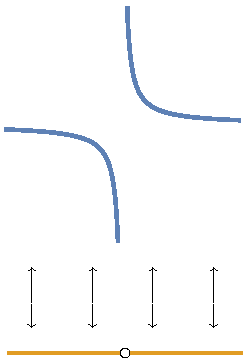
\includegraphics[width=\linewidth]{figures/affine-hyperbola-punctured-line-isomorphism.pdf}
}
因此, 即使 $X$ 并非自然地来自仿射簇, 它仍同构于一个自然来自仿射簇的拟射影簇. 上图描绘的是 $Y_{0}=\mathcal{V}(1-xy)\subseteq\mathbb{A}^{2}$ 与 $X_{0}=\mathbb{A}^{1}\setminus\{0\}\subseteq\mathbb{A}^{1}$ 之间的拟射影同构.
\end{Example}

由于通常希望簇的性质在同构下保持, 这一例子表明我们的术语陷入一种不理想的境地. 我们用一种直接的办法解决它: 只需修改\textquotedbl{}仿射簇\textquotedbl{}的定义, 要求它在拟射影簇的同构下保持不变.

\begin{Definition}{仿射簇}\leavevmode\label{def:affine-variety-as-quasiprojective-variety}
若拟射影簇 $X\subseteq\mathbb{P}^{m}$ 同构于某个拟射影簇 $Y\subseteq\mathbb{P}^{n}$, 且对某个 Zariski 闭子集 $Y_{0}\subseteq\mathbb{A}^{n}$ 有 $Y=j_{0}(Y_{0})$, 就称 $X$ 为\emph{仿射簇}.
\end{Definition}

尽管 Example~\ref{ex:punctured-affine-line-isomorphic-to-hyperbola} 中的拟射影簇 $\mathbb{P}^{1}\setminus\mathcal{V}(xy)$ 不\emph{等于}任何 Zariski 闭子集 $X_{0}\subseteq\mathbb{A}^{1}$ 的 $j_{0}(X_{0})$, 我们已经验证, $\mathbb{P}^{1}\setminus\mathcal{V}(xy)$ \emph{同构于}一个拟射影簇 $Y\subseteq\mathbb{P}^{2}$, 使对某个 Zariski 闭子集 $Y_{0}\subseteq\mathbb{A}^{2}$ 有 $Y=j_{0}(Y_{0})$. 因此根据 Definition~\ref{def:affine-variety-as-quasiprojective-variety}, 以下把拟射影簇 $\mathbb{P}^{1}\setminus\mathcal{V}(xy)$ 称为仿射簇.

这一术语却又引出了新的问题: 现在\textquotedbl{}仿射簇\textquotedbl{}指特定类型的拟射影簇, 那么原先称作仿射簇的对象, 即作为一族多项式的消没集而得到的 $\mathbb{A}^{n}$ 的子集, 应怎样称呼? 和上一段一样, 以下用 Zariski 拓扑的语言称呼它们.

\begin{BookTerminologyChange}\leavevmode\label{def:affine-vanishing-sets-are-called-zariski-closed-subsets}
对某个子集 $S\subseteq K[x_{1},\ldots,x_{n}]$, 形如 $\mathcal{V}_{\mathbb{A}}(S)$ 的 $\mathbb{A}^{n}$ 的子集, 以下称为 $\mathbb{A}^{n}$ 的 \emph{(Zariski) 闭子集}.
\end{BookTerminologyChange}

\BookPairedNote{
因此, 尽管 $\mathbb{A}^{1}\setminus\{0\}$ 不是 $\mathbb{A}^{1}$ 的 Zariski 闭子集, 从而按本书先前的术语不是仿射簇, 现在却可以称它为仿射簇, 因为根据 Definition~\ref{def:affine-variety-as-quasiprojective-variety}, 它作为拟射影簇是仿射的.
}{
注意, 这里已经开始不再区分子集 $X\subseteq\mathbb{A}^{n}$ 与相应的子集 $j_{0}(X)\subseteq\mathbb{P}^{n}$. 读者会逐渐习惯这种轻微的记号滥用.
}
这个具体例子是下一节将证明的一般结果的特例: 闭集 $X\subseteq\mathbb{A}^{n}$ 中使单个多项式不消没的点构成的子集, 总是仿射簇.

读者可能会问, 关于射影簇是否也需要类似的术语变更. 实际上, 在射影情形不需要, 因为射影簇已经在同构下保持. 更准确地说, 由本章稍后的讨论可知, 若 $X\subseteq\mathbb{P}^{m}$ 和 $Y\subseteq\mathbb{P}^{n}$ 为同构的拟射影簇, 则其中一个在其环境射影空间中 Zariski 闭当且仅当另一个也 Zariski 闭 (Corollary~\ref{cor:projectivity-invariant-under-quasiprojective-isomorphism}).

与此同时, 本节的最后一个目标是给出仿射空间中一个可以证明不是仿射簇的拟射影簇的例子.

\begin{Example}{$\mathbb{A}^{2}\setminus\{(0,0)\}$ 不是仿射簇}\leavevmode\label{ex:punctured-affine-plane-is-not-affine}
考察 $X_{0}=\mathbb{A}^{2}\setminus\{(0,0)\}$. 将它与拟射影簇 (Exercise~\ref{ex:punctured-affine-plane-as-projective-open-and-its-function-ring})
\[
  X=\mathbb{P}^{2}\setminus\mathcal{V}(x_{0}x_{1},x_{0}x_{2})
\]
等同. 反设 $X$ 是仿射簇, 则存在同构 $F:Y\to X$, 其中对某个闭子集 $Y_{0}\subseteq\mathbb{A}^{n}$ 有 $Y=j_{0}(Y_{0})$.

考察 $K[X]$ 中的正则函数 $G_{1}=x_{1}/x_{0}$ 和 $G_{2}=x_{2}/x_{0}$. 注意 $X$ 上不存在使 $G_{1}$ 和 $G_{2}$ 同时消没的点. 因此, $F^{*}G_{1}$ 和 $F^{*}G_{2}$ 在 $Y$ 上也没有共同的消没点. 由于 $K[Y]=K[Y_{0}]$ (Theorem~\ref{thm:regular-functions-on-affine-varieties-are-polynomial}), 对闭集 $Y_{0}\subseteq\mathbb{A}^{n}$ 应用零点定理得到 $K[Y]=\langle F^{*}G_{1},F^{*}G_{2}\rangle$ (见 Exercise~\ref{ex:regular-functions-with-no-common-zero-generate-unit}). 但是, 因为 $F^{*}:K[X]\to K[Y]$ 是同构 (Proposition~\ref{prop:quasiprojective-isomorphism-induces-regular-function-ring-isomorphism}), 可推出 $K[X]=\langle G_{1},G_{2}\rangle$.

另一方面, Lemma~\ref{lem:regular-functions-on-projective-open-subsets-are-global-quotients} 蕴含 (Exercise~\ref{ex:punctured-affine-plane-as-projective-open-and-its-function-ring})
\[
  K[X]\cong K[x_{1},x_{2}].
\]
理想 $\langle G_{1},G_{2}\rangle$ 在此同构下对应于 $\langle x_{1},x_{2}\rangle\subseteq K[x_{1},x_{2}]$, 因而为真理想, 与 $\langle G_{1},G_{2}\rangle=K[X]$ 矛盾. 这一矛盾意味着 $X$ 不可能是仿射簇.
\end{Example}

\BookExerciseHeading
\begin{BookExercises}
  \item\label{ex:laurent-polynomial-on-projective-conic-as-homogeneous-quotient} 令 $Y=\mathcal{V}(w^{2}-xy)\subseteq\mathbb{P}^{2}$, 如 Example~\ref{ex:regular-function-ring-of-punctured-projective-conic} 所示, 在那里已经看到
  \[
    K[Y]=K[x,x^{-1}].
  \]
  把与 $x^{4}-3x^{-1}\in K[x,x^{-1}]$ 对应的正则函数 $Y\to K$ 描述为 $K[w,x,y]$ 中同次数的齐次多项式的商.
  \item\label{ex:homogenize-polynomial-map-between-affine-curves-and-surfaces} 令 $X_{0}=\mathcal{V}_{\mathbb{A}}(x_{2}-x_{1}^{2})\subseteq\mathbb{A}^{2}$, $Y_{0}=\mathcal{V}_{\mathbb{A}}(y_{1}y_{2}-y_{3})\subseteq\mathbb{A}^{3}$. 考察如下给出的多项式映射 $X_{0}\to Y_{0}$:
  \[
    (a_{1},a_{2})\mapsto(a_{1}-a_{1}^{2},a_{1}+a_{2},a_{1}^{2}-a_{2}^{2}).
  \]
  用同次数的齐次多项式描述相应的拟射影簇之间的正则映射 $X\to Y$, 其中 $X=j_{0}(X_{0})\subseteq\mathbb{P}^{2}$ 且 $Y=j_{0}(Y_{0})\subseteq\mathbb{P}^{3}$.
  \item\label{ex:affine-polynomial-map-correspondence-is-bijective} 推广上一题中的构造, 证明 Corollary~\ref{cor:regular-maps-between-affine-varieties-are-polynomial} 陈述中的对应可逆, 因而是双射.
  \item\label{ex:punctured-affine-plane-as-projective-open-and-its-function-ring} 考察拟射影簇
  \[
    X=\mathbb{P}^{2}\setminus\mathcal{V}(x_{0}x_{1},x_{0}x_{2}).
  \]
  \begin{enumerate}
    \item 证明 $X=j_{0}(\mathbb{A}^{2}\setminus\{(0,0)\})$.
    \item 证明 $K[X]\cong K[x_{1},x_{2}]$.
  \end{enumerate}
  \item\label{ex:regular-functions-with-no-common-zero-generate-unit} 设 $X\subseteq\mathbb{A}^{n}$ 为闭集, $F_{1},\ldots,F_{k}\in K[X]$ 为在 $X$ 上没有共同消没点的正则函数. 用零点定理证明 $K[X]=\langle F_{1},\ldots,F_{k}\rangle$.
  \item\label{ex:positive-dimensional-projective-space-is-not-affine} 证明拟射影簇 $\mathbb{P}^{n}$ 对任何 $n>0$ 都不是仿射簇.
\end{BookExercises}

\section{仿射开集与局部性质}\label{sec:affine-opens-and-local-properties}

已经证明拟射影簇理论专化为仿射簇理论, 现在可以描述拟射影簇最有用的性质之一: 每个拟射影簇都是\textquotedbl{}局部仿射\textquotedbl{}的, 其确切含义将在本节说明. 这一事实的作用在于, 它使我们能把拟射影簇的许多性质, 例如维数和光滑性, 归结为仿射簇的相应性质. 本书第一部分已经详细建立了这些仿射性质.

证明每个拟射影簇都局部仿射的第一步, 是研究仿射空间的闭子集中的非消没集.

\begin{Proposition}{非消没集是仿射簇}\leavevmode\label{prop:nonvanishing-sets-in-affine-closed-sets-are-affine}
若 $X\subseteq\mathbb{A}^{n}$ 是 Zariski 闭集, 且 $f\in K[x_{1},\ldots,x_{n}]$, 则集合 $U(f)=X\setminus\mathcal{V}(f)$ 是仿射簇.
\end{Proposition}

Example~\ref{ex:punctured-affine-line-isomorphic-to-hyperbola} 展示了此结果的一个实例: 非消没集 $\mathbb{A}^{1}\setminus\mathcal{V}(x)$ 同构于闭集 $\mathcal{V}_{\mathbb{A}}(xy-1)\subseteq\mathbb{A}^{2}$. 更一般地, 类似的论证表明, 对任意 $f\in K[x_{1},\ldots,x_{n}]$, $\mathbb{A}^{n}\setminus\mathcal{V}(f)$ 同构于闭集 $\mathcal{V}(x_{n+1}f-1)\subseteq\mathbb{A}^{n+1}$. 这些特例为一般证明提供了范例, 现在给出证明.

\begingroup
\renewcommand{\AJProofBegin}{%
  \par\addvspace{\topsep}\noindent
  {\sffamily\bfseries\CJKfamily{pffont}Proof of Proposition~\ref{prop:nonvanishing-sets-in-affine-closed-sets-are-affine}}\enspace\ignorespaces
}
\begin{Proof}
令 $X\subseteq\mathbb{A}^{n}$ 为闭集, 从而可以写成
\[
  X=\mathcal{V}_{\mathbb{A}}(g_{1},\ldots,g_{m}),
\]
其中 $g_{1},\ldots,g_{m}\in K[x_{1},\ldots,x_{n}]$. 给定 $f\in K[x_{1},\ldots,x_{n}]$, 定义闭集 $Y\subseteq\mathbb{A}^{n+1}$ 为
\[
  Y=\mathcal{V}_{\mathbb{A}}(g_{1},\ldots,g_{m},x_{n+1}f-1).
\]
我们断言 $U(f)$ 与 $Y$ 作为拟射影簇同构. 由于 $Y$ 是仿射空间的闭子集, 这将蕴含 $U(f)$ 是仿射簇.

要看出 $U(f)\cong Y$, 考察投影映射
\[
  \begin{aligned}
    H:Y&\to U(f)\\
    (a_{1},\ldots,a_{n},a_{n+1})&\mapsto(a_{1},\ldots,a_{n}).
  \end{aligned}
\]
注意 (Exercise~\ref{ex:graph-of-inverse-polynomial-projection-is-bijective}), $H$ 为双射, 其逆 $H^{-1}$ 由下式给出:
\[
  (a_{1},\ldots,a_{n})\mapsto\left(a_{1},\ldots,a_{n},\frac{1}{f(a)}\right).
\]
只需再论证 $H$ 和 $H^{-1}$ 都正则. 为此, 将 $Y$ 和 $U(f)$ 分别与它们在 $\mathbb{P}^{n+1}$ 和 $\mathbb{P}^{n}$ 中的像等同. 令 $\overline{f}$ 为 $f$ 的齐次化, 并设 $\deg(\overline{f})=d$. 则 $H$ 对应于正则映射
\[
  [a_{0}:\cdots:a_{n}:a_{n+1}]\mapsto[a_{0}:\cdots:a_{n}],
\]
而稍加思考可知 $H^{-1}$ 对应于正则映射
\[
  [a_{0}:\cdots:a_{n}]\mapsto[a_{0}\overline{f}(a):\cdots:a_{n}\overline{f}(a):a_{0}^{d+1}].
\]
因此 $U(f)\cong Y$, 如所断言.
\end{Proof}
\endgroup

\BookPairedNoteLeft{
上述证明的关键在于, 转到射影空间后, 可以消去分母中的 $f(a)$.
}{
Proposition~\ref{prop:nonvanishing-sets-in-affine-closed-sets-are-affine} 表明, 仿射空间闭子集中的非消没集本身是仿射簇. 这并不对仿射空间的所有开子集成立. 例如, Example~\ref{ex:punctured-affine-plane-is-not-affine} 中遇到的拟射影簇 $\mathbb{A}^{2}\setminus\{(0,0)\}$ 在 $\mathbb{A}^{2}$ 中是开的, 但不是仿射簇.
}
现在利用 Proposition~\ref{prop:nonvanishing-sets-in-affine-closed-sets-are-affine} 证明本节的主要结果: 每个拟射影簇都局部同构于一个仿射簇, 即拟射影簇的每一点都包含在一个仿射开子簇中. 事实上, 我们证明更强的结果: 每个拟射影簇都能由有限多个仿射开子簇覆盖.

\begin{Theorem}{拟射影簇是局部仿射的}\leavevmode\label{thm:quasiprojective-varieties-have-finite-affine-open-covers}
设 $X$ 为拟射影簇. 则存在有限多个仿射开子簇 $U_{1},\ldots,U_{k}\subseteq X$, 使 $X=U_{1}\cup\cdots\cup U_{k}$. 特别地, 对每个 $p\in X$, 都存在仿射开子簇 $U\subseteq X$ 使 $p\in U$.
\end{Theorem}
\begin{Proof}
令 $X\subseteq\mathbb{P}^{n}$ 为拟射影簇. 按定义, 有
\[
  X=Y\cap(\mathbb{P}^{n}\setminus Z)=Y\setminus Z,
\]
其中 $Y,Z\subseteq\mathbb{P}^{n}$ 为射影簇. 对某些齐次多项式 $f_{1},\ldots,f_{k}\in K[x_{0},\ldots,x_{n}]$, 写成 $Z=\mathcal{V}(f_{1},\ldots,f_{k})$. 对每个 $i=1,\ldots,k$ 及每个 $j=0,\ldots,n$, 定义
\[
  U_{i,j}=(Y\setminus\mathcal{V}(f_{i}))\cap\mathbb{A}^{n}_{j}.
\]
注意 $Z=\mathcal{V}(f_{1},\ldots,f_{k})\subseteq\mathcal{V}(f_{i})$, 所以 $Y\setminus\mathcal{V}(f_{i})=X\setminus\mathcal{V}(f_{i})$. 因此, 对每个 $i$, $Y\setminus\mathcal{V}(f_{i})$ 是 $X$ 的开子簇. 又因为 $\mathbb{A}^{n}_{j}$ 在 $\mathbb{P}^{n}$ 中开, 对所有 $i,j$, $U_{i,j}$ 都是 $X$ 的开子簇. 此外, 注意
\[
  U_{i,j}=(Y\cap\mathbb{A}^{n}_{j})\setminus\mathcal{V}(f_{i,j}),
\]
其中 $f_{i,j}$ 是在 $f_{i}$ 中令 $x_{j}=1$ 得到的 $n$ 元多项式. 由于 $Y\cap\mathbb{A}^{n}_{j}$ 是 $\mathbb{A}^{n}_{j}$ 的闭子集, 由 Proposition~\ref{prop:nonvanishing-sets-in-affine-closed-sets-are-affine} 可知每个 $U_{i,j}$ 都是仿射簇. 定理现在由下式得到:
\[
  X=\bigcup_{\substack{1\le i\le k\\0\le j\le n}}U_{i,j},
\]
建议读者在 Exercise~\ref{ex:finite-affine-open-cover-from-defining-equations} 中验证这一等式, 从而证明 $X$ 的每一点都属于 (至少) 一个仿射开子簇 $U_{i,j}$.
\end{Proof}

回顾第~\ref{sec:quasiprojective-varieties}~节, 点 $p\in X$ 的\emph{邻域}是包含 $p$ 的 $X$ 的任一开子集. 因此, Theorem~\ref{thm:quasiprojective-varieties-have-finite-affine-open-covers} 可以重述为: \emph{拟射影簇的每一点都有一个仿射邻域}. 下面的例子具体说明这一定理.

\begin{Example}{$\mathbb{A}^{2}\setminus\{(0,0)\}$ 是局部仿射的}\leavevmode\label{ex:punctured-affine-plane-has-affine-open-cover}
令 $X=\mathbb{A}^{2}\setminus\{(0,0)\}$, 以通常的方式将它视为 $\mathbb{P}^{2}$ 中的拟射影簇. 由 Proposition~\ref{prop:nonvanishing-sets-in-affine-closed-sets-are-affine}, 子集
\[
  U=X\setminus\mathcal{V}(x)=\mathbb{A}^{2}\setminus\mathcal{V}(x)
\]
是仿射簇. 特别地, $U\cong\mathcal{V}(xz-1)\subseteq\mathbb{A}^{3}$, 同构由
\[
  (x,y)\mapsto\left(x,y,\frac{1}{x}\right)
\]
给出. 类似地,
\[
  V=X\setminus\mathcal{V}(y)=\mathbb{A}^{2}\setminus\mathcal{V}(y)
\]
也是仿射簇. $U$ 和 $V$ 都是 $X$ 的 Zariski 开子簇. 由于 $X$ 的每一点的 $x$ 坐标或 $y$ 坐标必有一个非零, 每一点都包含在 $U$ 或 $V$ 中. 这样便验证了拟射影簇 $\mathbb{A}^{2}\setminus\{(0,0)\}$ 的每一点都包含在一个仿射邻域中.
\end{Example}

如本节开头所说, Theorem~\ref{thm:quasiprojective-varieties-have-finite-affine-open-covers} 的作用在于, 它允许把拟射影簇某些性质的研究归结到仿射情形. 现在为这些性质命名.

\begin{Definition}{局部性质}\leavevmode\label{def:local-property-of-topological-spaces}
令 $\mathcal{C}$ 为一类拓扑空间. 若 $\mathcal{C}$ 上的性质 $\mathcal{P}$ 满足以下条件, 则称其为\emph{局部的}: 若 $X\in\mathcal{C}$, 且每个 $p\in X$ 都包含在具有性质 $\mathcal{P}$ 的开集 $U_{p}\subseteq X$ 中, 则 $X$ 具有性质 $\mathcal{P}$.
\end{Definition}

一个反例有助于理解这一定义: 仿射性不是拟射影簇类上的局部性质, 因为例如 $\mathbb{P}^{n}$ 不是仿射簇 (Exercise~\ref{ex:positive-dimensional-projective-space-is-not-affine}), 但 $\mathbb{P}^{n}$ 的每一点都包含在某个仿射开片中. 打个比方, 如果一个人的视力很差, 看不到任何给定点的一个小邻域之外的地方, 就不可能辨认自己站在仿射簇 $\mathbb{A}^{n}$ 中还是非仿射簇 $\mathbb{P}^{n}$ 中. 这有点像早期人类无法看出自己站的不是平坦地面构成的地球, 而是一个 (近似) 球形的地球.

另一方面, 光滑性是不可约拟射影簇类上的局部性质的一个例子, 如我们将在下一章看到的. 直观上, 若 $X$ 有一个奇点, 那么即使是 $X$ 中一个近视的居民, 只要站在这个点上, 也会知道它是奇点. 类似地, 具有某个特定维数是不可约簇的局部性质: 在不可约簇内可独立移动的方向数, 可以在任意一点的邻域中判定. 下一章将深入讨论这两个性质.

本节最后给出局部性质的两个有用结果, 下一节都会用到. 第一个引理说, 要验证拓扑空间的一个子集是闭的, 只须检查它在每一点的某个邻域中是闭的.

\begin{Lemma}{闭性是局部的}\leavevmode\label{lem:closedness-is-local}
设 $Y$ 为拓扑空间, $X\subseteq Y$ 为子集. 若每个 $p\in Y$ 都包含在一个开集 $U_{p}\subseteq Y$ 中, 使 $X\cap U_{p}$ 在 $U_{p}$ 中闭, 则 $X$ 在 $Y$ 中闭.
\end{Lemma}
\begin{Proof}
对每个 $p\in Y$, 固定开集 $U_{p}$, 使得 $p\in U_{p}$ 且 $X\cap U_{p}$ 在 $U_{p}$ 中闭. 由开集的定义, 对每个 $p$, 存在闭集 $Z_{p}\subseteq Y$, 使 $U_{p}=Y\setminus Z_{p}$. 由子空间拓扑的定义, 存在闭集 $Z'_{p}\subseteq Y$, 使 $X\cap U_{p}=Z'_{p}\cap U_{p}$. 现在断言
\[
  X=\bigcap_{p\in Y}(Z_{p}\cup Z'_{p}),
\]
由此可知 $X$ 在 $Y$ 中闭.

($\subseteq$) 假设 $q\in X$. 则对每个 $p\in Y$, 有 $q\in U_{p}$ 或 $q\notin U_{p}$. 若 $q\in U_{p}$, 则 $q\in X\cap U_{p}=Z'_{p}\cap U_{p}$, 故 $q\in Z'_{p}$. 若 $q\notin U_{p}$, 则 $q\in Z_{p}$. 因此无论哪种情形, 都有 $q\in Z_{p}\cup Z'_{p}$, 且这对所有 $p\in Y$ 成立.

($\supseteq$) 反过来, 假设对所有 $p\in Y$ 都有 $q\in Z_{p}\cup Z'_{p}$. 由于 $q\in U_{q}$, 有 $q\notin Z_{q}$. 因而 $q\in Z_{q}\cup Z'_{q}$ 蕴含 $q\in Z'_{q}$. 于是 $q\in Z'_{q}\cap U_{q}=X\cap U_{q}$, 所以 $q\in X$.
\end{Proof}

下一个引理断言, 正则性可以在定义域上局部检查.

\begin{Lemma}{正则性在定义域上是局部的}\leavevmode\label{lem:regularity-is-local-on-domain}
令 $X\subseteq\mathbb{P}^{m}$ 和 $Y\subseteq\mathbb{P}^{n}$ 为拟射影簇, $F:X\to Y$ 为映射. 若每个 $p\in X$ 都包含在一个开集 $U_{p}\subseteq X$ 中, 使限制 $F:U_{p}\to Y$ 正则, 则 $F$ 正则.
\end{Lemma}
\begin{Proof}
设映射 $F:X\to Y$ 满足引理的假设. 为证明 $F$ 正则, 令 $p\in X$. 按假设, 存在开集 $U_{p}\subseteq X$ 和同次数的齐次多项式 $g_{0},\ldots,g_{n}\in K[x_{0},\ldots,x_{m}]$, 使 $p\notin\mathcal{V}(g_{0},\ldots,g_{n})$, 且
\[
  F(a)=[g_{0}(a):\cdots:g_{n}(a)]
  \qquad\text{对所有 }a\in U_{p}\setminus\mathcal{V}(g_{0},\ldots,g_{n}).
\]
要使 $F$ 满足正则映射的定义, 上式须在整个 $X\setminus\mathcal{V}(g_{0},\ldots,g_{n})$ 上成立, 但它未必如此.

为解决这一问题, 选取齐次多项式 $f\in K[x_{0},\ldots,x_{n}]$, 使 $f$ 在闭集 $X\setminus U_{p}\subseteq X$ 上消没, 且 $f(p)\ne0$. 对每个 $i=0,\ldots,n$, 定义 $f_{i}=fg_{i}$. 注意两个函数 $[f_{0}:\cdots:f_{n}]$ 和 $[g_{0}:\cdots:g_{n}]$ 在它们都有定义之处取值相同, 但前者的定义域较小. 特别地, 由于 $f$ 在 $X\setminus U_{p}$ 上消没, 得
\[
  X\setminus\mathcal{V}(f_{0},\ldots,f_{n})
    =U_{p}\setminus\mathcal{V}(f_{0},\ldots,f_{n}).
\]
因此, 由构造可知 $p\notin X\setminus\mathcal{V}(f_{0},\ldots,f_{n})$, 且
\[
  F(a)=[f_{0}(a):\cdots:f_{n}(a)]
  \qquad\text{对所有 }a\in X\setminus\mathcal{V}(f_{0},\ldots,f_{n}),
\]
所以 $F$ 在 $p$ 处正则.
\end{Proof}

\BookExerciseHeading
\begin{BookExercises}
  \item\label{ex:graph-of-inverse-polynomial-projection-is-bijective} 令 $g_{1},\ldots,g_{m},f\in K[x_{0},\ldots,x_{n}]$, 定义
  \[
    \begin{aligned}
    X&=\mathcal{V}(g_{1},\ldots,g_{m})\subseteq\mathbb{A}^{n},\\
    Y&=\mathcal{V}(g_{1},\ldots,g_{m},x_{n+1}f-1)\subseteq\mathbb{A}^{n+1}.
    \end{aligned}
  \]
  证明函数
  \[
    \begin{aligned}
      \phi:Y&\to X\setminus\mathcal{V}(f)\\
      (a_{1},\ldots,a_{n},a_{n+1})&\mapsto(a_{1},\ldots,a_{n})
    \end{aligned}
  \]
  是双射, 并计算它的逆.
  \item\label{ex:regular-function-ring-of-principal-open-is-localization} 令 $X\subseteq\mathbb{A}^{n}$ 为闭集, $f\in K[x_{1},\ldots,x_{n}]$. 置 $F=[f]\in K[X]$, 证明
  \[
    K[X\setminus\mathcal{V}(f)]=\frac{K[X][z]}{\langle zF-1\rangle}.
  \]
  (当 $a$ 在 $R$ 中不是幂零元时, 通常用 $R[a^{-1}]$ 记环 $R[z]/\langle za-1\rangle$. 因此, 有 $K[X\setminus\mathcal{V}(f)]=K[X][F^{-1}]$.)
  \item\label{ex:finite-affine-open-cover-from-defining-equations} 设 $Y,Z\subseteq\mathbb{P}^{n}$ 为射影簇, 且 $Z=\mathcal{V}(f_{1},\ldots,f_{k})$. 对每个 $i=1,\ldots,k$ 和 $j=0,\ldots,n$, 定义
  \[
    U_{i,j}=(Y\setminus\mathcal{V}(f_{i}))\cap\mathbb{A}^{n}_{j}.
  \]
  证明
  \[
    Y\setminus Z=\bigcup_{\substack{1\le i\le k\\0\le j\le n}}U_{i,j}.
  \]
  \item\label{ex:affine-open-cover-of-punctured-affine-space} 构造 $\mathbb{A}^{n}\setminus\{(0,\ldots,0)\}$ 的有限仿射开覆盖.
  \item\label{ex:affine-open-cover-of-open-projective-quadric} 令 $Y=\mathcal{V}(x^{2}+y^{2}-zw)\subseteq\mathbb{P}^{3}$, $Z=\mathcal{V}(x,y,z)\subseteq\mathbb{P}^{3}$. 构造 $X=Y\setminus Z$ 的有限仿射开覆盖.
  \item\label{ex:projective-hypersurface-complement-is-affine} 令 $f\in K[x_{0},\ldots,x_{n}]$ 为非常数齐次多项式. 证明 $\mathbb{P}^{n}\setminus\mathcal{V}(f)$ 是仿射簇. (提示: 使用一个 Veronese 映射.)
\end{BookExercises}

\section{正则映射的连续性}\label{sec:continuity-of-regular-maps}

我们已经引入正则映射, 作为拟射影簇情形中的\textquotedbl{}保结构\textquotedbl{}映射. 既然每个拟射影簇都配有 Zariski 拓扑, 自然会问: 正则映射是否保持这一拓扑的\textquotedbl{}结构\textquotedbl{}? 本节致力于回答这一问题. 我们引入拓扑学中的保结构映射, 即连续映射, 然后证明拟射影簇之间的正则映射关于 Zariski 拓扑是连续的.

先回顾熟悉的连续性概念. 初次接触连续性通常是在微积分中研究函数 $f:\mathbb{R}\to\mathbb{R}$ 时. 在那里, 可以先把连续函数介绍为不用提起笔就能画出图像的函数, 但这种说法相当不正式. 为使之严格, 学生接着要理解连续性的 $\epsilon$-$\delta$ 定义: 对每个 $x_{0}\in\mathbb{R}$ 和每个 $\epsilon>0$, 存在 $\delta>0$, 使 $|x-x_{0}|<\delta$ 蕴含 $|f(x)-f(x_{0})|<\epsilon$.

虽然久而久之 $\epsilon$-$\delta$ 定义会变得直观, 它仍有些繁琐. 幸运的是, 连续性有一个优雅的拓扑刻画: 函数 $f:\mathbb{R}\to\mathbb{R}$ 连续 (按 $\epsilon$-$\delta$ 定义), 当且仅当对每个 Euclid 开集 $V\subseteq\mathbb{R}$, $f^{-1}(V)$ 在 $\mathbb{R}$ 中是 Euclid 开集. 这一刻画的重要性在于, 它引出了连续性的纯拓扑表述. 即使没有度量距离的方法, 这个表述仍有意义, 从而得到以下一般的连续性概念.

\begin{Definition}{连续映射}\leavevmode\label{def:continuous-map-of-topological-spaces}
令 $X,Y$ 为拓扑空间. 若对每个开集 $V\subseteq Y$, 原像 $F^{-1}(V)$ 在 $X$ 中开, 则称映射 $F:X\to Y$ 为\emph{连续的}.
\end{Definition}

虽然通常用开集定义连续性, 正如这里所做的那样, 也可以用闭集重新表述连续性. 特别地 (Exercise~\ref{ex:equivalent-open-and-closed-characterizations-of-continuity}), 映射 $F:X\to Y$ 连续, 当且仅当对每个闭集 $Z\subseteq Y$, $F^{-1}(Z)$ 在 $X$ 中闭. 现在用第二种表述陈述本节的主要结果.

\begin{Theorem}{正则映射是连续的}\leavevmode\label{thm:regular-maps-are-zariski-continuous}
令 $F:X\to Y$ 为拟射影簇之间的正则映射. 若 $Z$ 在 $Y$ 中闭, 则 $F^{-1}(Z)$ 在 $X$ 中闭.
\end{Theorem}
\begin{Proof}
令 $X\subseteq\mathbb{P}^{m}$ 和 $Y\subseteq\mathbb{P}^{n}$ 为拟射影簇, $F:X\to Y$ 为正则映射. 给定闭子簇 $Z\subseteq Y$, 我们要证明 $F^{-1}(Z)$ 在 $X$ 中闭. 由 Lemma~\ref{lem:closedness-is-local}, 只须证明 $X$ 的每个点 $p$ 都包含在某个邻域 $U_{p}$ 中, 使 $F^{-1}(Z)\cap U_{p}$ 在 $U_{p}$ 中闭.

考察点 $p\in X$. 由正则映射的定义, 选取同次数的齐次多项式 $f_{0},\ldots,f_{n}\in K[x_{0},\ldots,x_{m}]$, 使 $p\notin\mathcal{V}(f_{0},\ldots,f_{n})$, 且
\[
  F(a)=[f_{0}(a):\cdots:f_{n}(a)]
  \qquad\text{对所有 }a\in X\setminus\mathcal{V}(f_{0},\ldots,f_{n}).
\]
置 $U_{p}=X\setminus\mathcal{V}(f_{0},\ldots,f_{n})$. 则 $U_{p}$ 在 $X$ 中开且包含 $p$. 考察由 $F_{p}=[f_{0}:\cdots:f_{n}]$ 整体定义的正则函数 $F_{p}:U_{p}\to\mathbb{P}^{n}$. 注意
\[
  F^{-1}(Z)\cap U_{p}=F_{p}^{-1}(Z)=F_{p}^{-1}(\overline{Z}),
\]
其中 $\overline{Z}$ 是 $Z$ 在 $\mathbb{P}^{n}$ 中的射影闭包. 最后一个等式成立, 是因为 $Z$ 在 $Y$ 中闭, 因而 $Z=\overline{Z}\cap Y$. 由于 $\overline{Z}$ 在 $\mathbb{P}^{n}$ 中闭, 存在齐次多项式 $g_{1},\ldots,g_{k}\in K[y_{1},\ldots,y_{n}]$, 使 $\overline{Z}=\mathcal{V}(g_{1},\ldots,g_{k})$. 于是, 对每个 $i=1,\ldots,k$, $g_{i}(f_{0},\ldots,f_{n})$ 都是 $K[x_{1},\ldots,x_{m}]$ 中的齐次多项式. 稍加思考 (Exercise~\ref{ex:preimage-of-projective-vanishing-set-under-polynomial-map}) 可知
\[
  F_{p}^{-1}(\overline{Z})
  =U_{p}\cap\mathcal{V}\bigl(g_{1}(f_{0},\ldots,f_{n}),\ldots,g_{k}(f_{0},\ldots,f_{n})\bigr).
\]
所以 $F^{-1}(Z)\cap U_{p}=F_{p}^{-1}(\overline{Z})$ 在 $U_{p}$ 中闭, 如所需.
\end{Proof}

连续映射是拓扑学中的保结构映射. 因此, 有连续逆映射的连续映射给出了拓扑空间之间的一种自然等价概念, 称为同胚.

\begin{Definition}{同胚}\leavevmode\label{def:homeomorphism-of-topological-spaces}
令 $X,Y$ 为拓扑空间. 从 $X$ 到 $Y$ 的\emph{同胚}是具有连续逆映射 $G:Y\to X$ 的连续映射 $F:X\to Y$. 若 $X,Y$ 之间存在一个同胚, 就称 $X$ 与 $Y$ \emph{同胚}.
\end{Definition}

由于拟射影簇的同构是具有正则逆映射的正则映射, Theorem~\ref{thm:regular-maps-are-zariski-continuous} 蕴含, 拟射影簇的同构 $F:X\to Y$ 是关于 $X,Y$ 上 Zariski 拓扑的同胚. 这一观察体现在下述结果的前两条 (等价的) 断言中.

\begin{Corollary}{同构使子簇一一对应}\leavevmode\label{cor:quasiprojective-isomorphisms-identify-subvarieties}
若 $F:X\to Y$ 为拟射影簇的同构, 且 $Z\subseteq X$, 则下列断言成立.
\begin{enumerate}[label=\arabic*.]
  \item $Z$ 在 $X$ 中开, 当且仅当 $F(Z)$ 在 $Y$ 中开.
  \item $Z$ 在 $X$ 中闭, 当且仅当 $F(Z)$ 在 $Y$ 中闭.
  \item $Z$ 是 $X$ 的子簇, 当且仅当 $F(Z)$ 是 $Y$ 的子簇.
\end{enumerate}
此外, 若 $Z$ 是 $X$ 的子簇, 则限制 $F|_{Z}:Z\to F(Z)$ 是拟射影簇的同构.
\end{Corollary}
\begin{Proof}
Exercise~\ref{ex:isomorphisms-identify-open-closed-and-locally-closed-subsets}.
\end{Proof}

本节余下部分用 Theorem~\ref{thm:regular-maps-are-zariski-continuous} 建立正则映射和同构的其他刻画. 这些刻画只用连续性和正则函数表述, 不涉及拟射影簇所在的环境射影空间. 正如本节最后将讨论的, 这些刻画使我们更接近理解拟射影簇的真正内在性质.

\begin{Proposition}{正则映射的刻画}\leavevmode\label{prop:characterize-regular-maps-by-continuity-and-pullback}
令 $X\subseteq\mathbb{P}^{m}$ 和 $Y\subseteq\mathbb{P}^{n}$ 为拟射影簇. 映射 $F:X\to Y$ 正则, 当且仅当满足以下两个条件:
\begin{enumerate}[label=\arabic*.]
  \item $F$ 关于 Zariski 拓扑连续;
  \item 对每个开集 $V\subseteq Y$ 及每个正则函数 $G\in K[V]$, 函数 $G\circ F$ 在 $F^{-1}(V)$ 上正则.
\end{enumerate}
\end{Proposition}
\begin{Proof}
\BookPairedNote{
先假设映射 $F:X\to Y$ 正则. 则命题陈述中的条件 1 来自 Theorem~\ref{thm:regular-maps-are-zariski-continuous}. 条件 2 来自这样的观察: $F$ 在开集 $F^{-1}(V)$ 上的限制仍正则, 而且正则映射诱导的拉回是良定义的 (Exercise~\ref{ex:pullback-regular-functions-is-algebra-homomorphism}).
}{
见 Exercise~\ref{ex:regular-maps-via-affine-open-covers}, 其中还用仿射开覆盖刻画了正则映射.
}
因此, 只需再证明这一双向陈述的另一个方向.

假设 $F:X\to Y$ 满足命题陈述中的条件 1 和 2. 我们要证明 $F$ 正则. 由 Lemma~\ref{lem:regularity-is-local-on-domain}, 只须证明每个 $p\in X$ 都包含在某个开集 $U_{p}\subseteq X$ 中, 使限制 $F:U_{p}\to Y$ 正则. 令 $p\in X$. 不妨假设 $F(p)\notin\mathcal{V}(y_{0})$, 先定义 $U=F^{-1}(Y\cap\mathbb{A}^{n}_{0})$. 这是 $X$ 的开集 (由条件 1), 且包含 $p$ (因为 $F(p)\notin\mathcal{V}(y_{0})$).

由于对每个 $a\in U$ 有 $F(a)\notin\mathcal{V}(y_{0})$, 可以对每个 $F(a)$ 的齐次坐标作缩放, 使 $y_{0}$ 坐标为 $1$. 因此, 存在唯一的函数 $F_{1},\ldots,F_{n}:U\to K$, 使
\begin{equation}\label{eq:regular-map-in-target-affine-coordinates}
  F(a)=[1:F_{1}(a):\cdots:F_{n}(a)]\qquad\text{对每个 }a\in U.
\end{equation}
换句话说, $F_{i}=(y_{i}/y_{0})\circ F$. 注意 $y_{1}/y_{0},\ldots,y_{n}/y_{0}$ 是 $\mathbb{A}^{n}_{0}$ 上的正则函数. 由条件 2 可知, 各复合 $(y_{i}/y_{0})\circ F=F_{i}$ 在 $U$ 上正则. 由于 $p\in U$, 由正则函数的定义, 对所有 $i=1,\ldots,n$, 都存在同次数的齐次多项式 $g_{i},h_{i}\in K[x_{0},\ldots,x_{m}]$, 使 $h_{i}(p)\ne0$, 且
\begin{equation}\label{eq:target-affine-coordinate-is-local-quotient}
  F_{i}(a)=g_{i}(a)/h_{i}(a)
  \qquad\text{对所有 }a\in U\setminus\mathcal{V}(h_{i}).
\end{equation}
定义 $f_{0}=h_{1}\cdots h_{n}$, 对 $i=1,\ldots,n$ 定义 $f_{i}=f_{0}g_{i}/h_{i}$, 并置 $U_{p}=U\setminus\mathcal{V}(f_{0})$. 则 $U_{p}$ 是包含 $p$ 的 $X$ 的开集. 稍加思考可知多项式 $f_{0},\ldots,f_{n}\in K[x_{0},\ldots,x_{m}]$ 都是同次数的齐次多项式, 而且由 \eqref{eq:regular-map-in-target-affine-coordinates} 和 \eqref{eq:target-affine-coordinate-is-local-quotient} 可知
\[
  F(a)=[f_{0}(a):\cdots:f_{n}(a)]\qquad\text{对所有 }a\in U_{p}.
\]
因此已证明 $F:U_{p}\to Y$ 正则.

这样, 对每个 $p\in X$, 我们都构造了开集 $U_{p}\subseteq X$, 使限制 $F:U_{p}\to Y$ 正则. 因而 $F:X\to Y$ 正则.
\end{Proof}

在上一结果的基础上, 现在用开集及开集上的正则函数刻画拟射影簇之间的同构.

\begin{Corollary}{同构的刻画}\leavevmode\label{cor:characterize-quasiprojective-isomorphisms-by-local-rings-of-functions}
令 $X,Y$ 为拟射影簇. 映射 $F:X\to Y$ 是同构, 当且仅当满足以下两个条件:
\begin{enumerate}[label=\arabic*.]
  \item $F$ 关于 Zariski 拓扑是同胚;
  \item 对每个开集 $V\subseteq Y$, 映射 $G\mapsto G\circ F$ 是从 $K[V]$ 到 $K[F^{-1}(V)]$ 的良定义的 $K$-代数同构.
\end{enumerate}
\end{Corollary}
\begin{Proof}
\BookPairedNote{
先假设 $F$ 为同构. 则 $F$ 是正则映射并有正则逆映射, 由 Theorem~\ref{thm:regular-maps-are-zariski-continuous} 可知 $F$ 是同胚.
}{
见 Exercise~\ref{ex:quasiprojective-isomorphisms-via-affine-open-cover}, 其中还用仿射开覆盖刻画了同构.
}
此外, 对每个开集 $V\subseteq Y$, $F$ 限制为同构 $F:F^{-1}(V)\to V$. 由 Proposition~\ref{prop:quasiprojective-isomorphism-induces-regular-function-ring-isomorphism} 可知 $F^{*}:K[V]\to K[F^{-1}(V)]$ 是同构. 这就证明了双向叙述的一个方向.

反过来, 假设 $F:X\to Y$ 满足命题陈述中的两个条件. 因为 $F$ 连续, 且对每个 $G\in K[V]$ 有 $G\circ F\in K[F^{-1}(V)]$, 由 Proposition~\ref{prop:characterize-regular-maps-by-continuity-and-pullback} 可知 $F$ 正则. 又因为 $F$ 是同胚, 它有连续逆映射 $F^{-1}:Y\to X$. 只需证明 $F^{-1}$ 也正则.

令 $U\subseteq X$ 为开集. 将条件 2 应用于开集 $F(U)\subseteq Y$, 可知 $G\mapsto G\circ F$ 给出同构 $K[F(U)]\to K[U]$. 由此同态的满射性, 对每个 $H\in K[U]$, 都存在 $G\in K[F(U)]$ 使 $H=G\circ F$. 特别地,
\[
  H\circ F^{-1}=G\circ F\circ F^{-1}=G\in K[F(U)].
\]
\BookPairedNoteLeft{
我们的论证没有用到 $G\mapsto G\circ F$ 的单射性. 这一单射性由 $F$ 的满射性推出.
}{
总而言之, 已验证对每个开集 $U\subseteq X$ 和每个正则函数 $H\in K[U]$, 复合 $H\circ F^{-1}$ 在集合 $F(U)=(F^{-1})^{-1}(U)$ 上正则.
}
由于 $F^{-1}$ 也连续, 由 Proposition~\ref{prop:characterize-regular-maps-by-continuity-and-pullback} 可知 $F^{-1}$ 正则, 如所需.
\end{Proof}

到目前为止的发展使我们开始窥见拟射影簇的内在性质. 与仿射簇的情形不同, 仿射簇的内在性质由一个 $K$-代数 (它的坐标环) 完全确定, 而一般拟射影簇的内在性质既有拓扑的一面, 又有代数的一面, 两者都必须考虑. 更具体地说, 拟射影簇 $X$ 的本质数据既包括 $X$ 中开集的信息 ($X$ 上的一个拓扑), 也包括每个开集 $U\subseteq X$ 上正则函数环的信息 ($X$ 上的一个 $K$-代数\textquotedbl{}层\textquotedbl{}). 由 Corollary~\ref{cor:characterize-quasiprojective-isomorphisms-by-local-rings-of-functions}, 拟射影簇之间的函数 $F:X\to Y$ 是同构, 当且仅当 $F$ 是同胚, 即 $F$ 保持拓扑结构, 并且对每个开集 $V\subseteq Y$, $F^{*}:K[V]\to K[F^{-1}(V)]$ 是 $K$-代数的同构, 即 $F$ 保持代数结构.

在仿射情形, 情况简单得多: 要知道仿射情形中的一个映射是否为同构, 只须检查其拉回是否为 $K$-代数的同构, 随即无须另行验证就得到拓扑同胚. 换句话说, 在仿射情形, 代数完全支配拓扑 (以及所有其他内在数据). 然而, 如我们已经看到的 (例如 Example~\ref{ex:regular-functions-on-projective-space-are-constant}), 更一般的拟射影情形并非如此: 整体正则函数的 $K$-代数通常不能刻画簇的全部内在性质. 研究一般的拟射影簇时, 我们需要其拓扑结构, 因为它实质上记录了局部仿射邻域 (在那里, 代数完全支配拓扑) 如何粘合为更整体的对象.

\BookExerciseHeading
\begin{BookExercises}
  \item\label{ex:equivalent-open-and-closed-characterizations-of-continuity} 令 $X,Y$ 为拓扑空间, $F:X\to Y$ 为映射. 证明对 $Y$ 中每个开集 $V$, $F^{-1}(V)$ 在 $X$ 中开, 当且仅当对 $Y$ 中每个闭集 $Z$, $F^{-1}(Z)$ 在 $X$ 中闭.
  \item\label{ex:restrict-domain-or-change-codomain-of-continuous-map} 令 $F:X\to Y$ 为拓扑空间之间的连续映射.
  \begin{enumerate}
    \item 令 $Z$ 为 $X$ 的子空间, 证明限制定义域给出连续映射 $F:Z\to Y$.
    \item 令 $Z$ 为以 $Y$ 为子空间的拓扑空间. 证明扩大陪域给出连续映射 $F:X\to Z$.
    \item 令 $Z$ 为 $Y$ 中包含 $F(X)$ 的子空间. 证明限制陪域给出连续映射 $F:X\to Z$.
  \end{enumerate}
  \item\label{ex:preimage-of-projective-vanishing-set-under-polynomial-map} 令 $X\subseteq\mathbb{P}^{m}$ 为拟射影簇, $f_{0},\ldots,f_{n}\in K[x_{1},\ldots,x_{m}]$ 为同次数的齐次多项式, 使得
  \[
    \mathcal{V}(f_{0},\ldots,f_{n})\cap X=\varnothing.
  \]
  若 $F=[f_{0}:\cdots:f_{n}]:X\to\mathbb{P}^{n}$ 且对某些 $g_{1},\ldots,g_{k}\in K[y_{1},\ldots,y_{n}]$, 有 $Z=\mathcal{V}(g_{1},\ldots,g_{k})\subseteq\mathbb{P}^{n}$, 证明
  \[
    F^{-1}(Z)=X\cap\mathcal{V}\bigl(g_{1}(f_{0},\ldots,f_{n}),\ldots,g_{k}(f_{0},\ldots,f_{n})\bigr).
  \]
  \item\label{ex:isomorphisms-identify-open-closed-and-locally-closed-subsets} 证明 Corollary~\ref{cor:quasiprojective-isomorphisms-identify-subvarieties}.
  \item\label{ex:irreducibility-invariant-under-quasiprojective-isomorphism} 证明不可约性是拟射影簇的内在性质. 换句话说, 若 $X,Y$ 是同构的拟射影簇, 证明 $X$ 不可约当且仅当 $Y$ 不可约.
  \item\label{ex:continuous-image-of-irreducible-subspace-is-irreducible} 令 $F:X\to Y$ 为拓扑空间之间的连续映射. 若 $Z$ 是 $X$ 的不可约子空间, 证明 $F(Z)$ 是 $Y$ 的不可约子空间.
  \item\label{ex:vanishing-locus-of-regular-functions-is-closed} 令 $X$ 为拟射影簇, $S\subseteq K[X]$ 为一族正则函数. 定义
  \[
    \mathcal{V}_{X}(S)=\{a\in X\mid F(a)=0\text{ 对所有 }F\in S\}.
  \]
  证明 $\mathcal{V}_{X}(S)$ 在 $X$ 中闭.
  \item\label{ex:regular-maps-via-affine-open-covers} 令 $F:X\to Y$ 为拟射影簇之间的映射. 证明 $F$ 正则, 当且仅当存在仿射开覆盖
  \[
    X=U_{1}\cup\cdots\cup U_{k}\qquad\text{和}\qquad
    Y=V_{1}\cup\cdots\cup V_{\ell},
  \]
  使得对每个 $i\in\{1,\ldots,k\}$, 都存在 $j\in\{1,\ldots,\ell\}$ 使 $U_{i}\subseteq F^{-1}(V_{j})$, 且限制
  \[
    F|_{U_{i}}:U_{i}\to V_{j}
  \]
  是仿射簇之间的正则映射.
  \item\label{ex:quasiprojective-isomorphisms-via-affine-open-cover} 令 $F:X\to Y$ 为拟射影簇之间的双射. 证明 $F$ 为同构, 当且仅当存在仿射开覆盖
  \[
    X=U_{1}\cup\cdots\cup U_{k},
  \]
  使对每个 $i$, $F(U_{i})$ 在 $Y$ 中开, 且限制 $F$ 给出同构 $U_{i}\cong F(U_{i})$.
\end{BookExercises}

\section{积与图像}\label{sec:quasiprojective-products-and-graphs}

现在转向拟射影簇的积, 为研究正则映射的图像做准备. 图像将在下一节起核心作用. 为了说明拟射影情形下积的含义, 先回顾第~\ref{sec:products-and-segre-maps}~节的 Segre 映射
\[
  S_{m,n}:\mathbb{P}^{m}\times\mathbb{P}^{n}\to\mathbb{P}^{(m+1)(n+1)-1}.
\]
这是一个单射, 将一对射影簇的积 $X\times Y$ 送到 $\mathbb{P}^{(m+1)(n+1)-1}$ 中的一个射影簇. 这允许我们将 $X\times Y$ 与它在 $S_{m,n}$ 下的像等同, 从而赋予它射影簇结构. 基于大致相同的理由, 拟射影簇也有类似的结果.

\begin{Proposition}{拟射影簇的积}\leavevmode\label{prop:segre-image-of-quasiprojective-product}
若 $X\subseteq\mathbb{P}^{m}$ 和 $Y\subseteq\mathbb{P}^{n}$ 是拟射影簇, 则 Segre 映射 $S_{m,n}$ 限制为从 $X\times Y$ 到 $\mathbb{P}^{(m+1)(n+1)-1}$ 中的一个拟射影簇上的单射.
\end{Proposition}
\begin{Proof}
Proposition~\ref{prop:segre-map-injective-with-determinantal-image} 表明 $S_{m,n}$ 为单射, 所以只需证明 $S_{m,n}(X\times Y)$ 是拟射影簇. 为此, 首先利用 $X$ 为拟射影簇的假设, 写 $X=Z\setminus Z'$ 且 $Y=W\setminus W'$, 其中 $Z,Z'$ 在 $\mathbb{P}^{m}$ 中闭, $W,W'$ 在 $\mathbb{P}^{n}$ 中闭. 从集合论来看, 注意
\[
  X\times Y=(Z\times W)\setminus\bigl((Z\times W')\cup(Z'\times W)\bigr).
\]
由于 $S_{m,n}$ 为单射, 得到
\[
  S_{m,n}(X\times Y)=S_{m,n}(Z\times W)
   \setminus\bigl(S_{m,n}(Z\times W')\cup S_{m,n}(Z'\times W)\bigr).
\]
由 Proposition~\ref{prop:segre-map-restricts-to-product-of-projective-varieties}, 集合 $S_{m,n}(Z\times W)$, $S_{m,n}(Z\times W')$ 和 $S_{m,n}(Z'\times W)$ 都闭. 这表明 $S_{m,n}(X\times Y)$ 是一个闭集在另一个闭集中的补集, 换句话说, 它是拟射影簇.
\end{Proof}

据此命题, 可以将 $X\times Y$ 与 $S_{m,n}(X\times Y)$ 等同, 从而在拟射影簇的范畴内定义积的含义.

\begin{Definition}{拟射影簇的积}\leavevmode\label{def:product-of-quasiprojective-varieties}
若 $X\subseteq\mathbb{P}^{m}$ 和 $Y\subseteq\mathbb{P}^{n}$ 为拟射影簇, 则它们的\emph{积} $X\times Y$ (作为拟射影簇) 是拟射影簇
\[
  S_{m,n}(X\times Y)\subseteq\mathbb{P}^{(m+1)(n+1)-1}.
\]
\end{Definition}

应该停下来确认, 积的这一定义与我们先前在仿射和射影情形下的概念一致. 在射影情形下, 由定义立即可见它们一致. 在仿射情形下, 只须证明 $S_{m,n}$ 限制为从 $\mathbb{A}^{m+n}=\mathbb{A}^{m}_{0}\times\mathbb{A}^{n}_{0}$ 到其像上的 (拟射影簇的) 同构 (Exercise~\ref{ex:segre-map-restricts-to-affine-product-isomorphism}).

现在, 在拟射影簇的范畴内, 可以说明射影簇与仿射簇的积等对象的含义, 并且可以讨论所得积中的闭子集与开子集.

\begin{Example}{积 $\mathbb{P}^{1}\times\mathbb{A}^{2}$}\leavevmode\label{ex:product-of-projective-line-and-affine-plane}
考察位于 $\mathbb{P}^{1}\times\mathbb{P}^{2}$ 中的积 $\mathbb{P}^{1}\times\mathbb{A}^{2}$. 按定义, Segre 映射 $S_{1,2}:\mathbb{P}^{1}\times\mathbb{P}^{2}\to\mathbb{P}^{5}$ 由下式给出:
\[
  S_{1,2}([a_{0}:a_{1}],[b_{0}:b_{1}:b_{2}])
  =[a_{0}b_{0}:a_{0}b_{1}:a_{0}b_{2}:a_{1}b_{0}:a_{1}b_{1}:a_{1}b_{2}],
\]
相应地将 $\mathbb{P}^{5}$ 上的坐标记为 $[z_{00}:z_{01}:z_{02}:z_{10}:z_{11}:z_{12}]$. 有 $\mathbb{A}^{2}=\mathbb{A}^{2}_{0}=\mathbb{P}^{2}\setminus\mathcal{V}(y_{0})$, 读者可验证
\[
  S_{1,2}(\mathbb{P}^{1}\times\mathcal{V}(y_{0}))
    =S_{1,2}(\mathbb{P}^{1}\times\mathbb{P}^{2})\cap\mathcal{V}(z_{00},z_{10}).
\]
结合此式与 Proposition~\ref{prop:segre-map-injective-with-determinantal-image} 中 $S_{1,2}(\mathbb{P}^{1}\times\mathbb{P}^{2})$ 的表达式, 得到 $S_{1,2}(\mathbb{P}^{1}\times\mathbb{A}^{2})$ 是 $\mathbb{P}^{5}$ 中由下式给出的拟射影簇:
\begin{equation}\label{eq:segre-description-of-projective-line-times-affine-plane}
  \begin{aligned}
  &\mathcal{V}(z_{00}z_{11}-z_{10}z_{01},\ 
      z_{00}z_{12}-z_{10}z_{02},\ z_{01}z_{12}-z_{11}z_{02})\\
  &\qquad{}\setminus\mathcal{V}(z_{00},z_{10}).
  \end{aligned}
\end{equation}
依照 Definition~\ref{def:product-of-quasiprojective-varieties}, 将这个拟射影簇记为 $\mathbb{P}^{1}\times\mathbb{A}^{2}$. 那么, $\mathbb{P}^{1}\times\mathbb{A}^{2}$ 的一个闭子集的例子是集合
\[
  Z=\{([a_{0}:a_{1}],(b_{1},b_{2}))\mid a_{0}-a_{1}=0,\ b_{1}-1=0\},
\]
因为 $S_{1,2}$ 将 $Z$ 与 \eqref{eq:segre-description-of-projective-line-times-affine-plane} 同射影簇 $\mathcal{V}(z_{00}-z_{01},z_{01}-z_{10})$ 的交等同; 见 Exercise~\ref{ex:verify-closed-subset-of-projective-line-times-affine-plane}.
\end{Example}

若 $X\subseteq\mathbb{P}^{m}$ 和 $Y\subseteq\mathbb{P}^{n}$ 为拟射影簇, 则 $X\times Y$ 上的 Zariski 拓扑是从 $\mathbb{P}^{m}\times\mathbb{P}^{n}$ 继承的子空间拓扑. 如 Proposition~\ref{prop:projective-subvarieties-of-product-are-vanishing-sets} 所见, $\mathbb{P}^{m}\times\mathbb{P}^{n}$ 的闭集恰是 $K[x_{0},\ldots,x_{m},y_{0},\ldots,y_{n}]$ 中多项式族的消没集. 因此, $X\times Y$ 的闭子集对应于形如
\[
  (X\times Y)\cap\mathcal{V}(S)
\]
的交集, 其中 $S\subseteq K[x_{0},\ldots,x_{m},y_{0},\ldots,y_{n}]$.

为下一节的发展作准备, 现在转来讨论正则映射的图像. 这自然地推广了微积分中学习的实值函数图像的概念.

\begin{Definition}{正则映射的图像}\leavevmode\label{def:graph-of-quasiprojective-regular-map}
令 $F:X\to Y$ 为拟射影簇之间的正则映射. $F$ 的\emph{图像}是集合
\[
  \Gamma_{F}=\{(a,b)\in X\times Y\mid b=F(a)\}\subseteq X\times Y.
\]
\end{Definition}

例如, 若 $F:\mathbb{A}^{1}_{\mathbb{R}}\to\mathbb{A}^{1}_{\mathbb{R}}$ 是由 $F(a)=a^{2}$ 定义的多项式映射, 则图像 $\Gamma_{F}$ 就是 $\mathbb{A}^{1}_{\mathbb{R}}\times\mathbb{A}^{1}_{\mathbb{R}}=\mathbb{A}^{2}_{\mathbb{R}}$ 中通常的抛物线.

再来看一个略一般的例子.

\begin{Example}{一个正则映射的图像}\leavevmode\label{ex:graph-of-map-from-punctured-projective-line}
令 $X=\mathbb{P}^{1}\setminus\mathcal{V}(x_{0}x_{1})$, $Y=\mathbb{P}^{1}$. 则由
\[
  F([a_{0}:a_{1}])=[a_{0}a_{1}:a_{0}^{2}+a_{1}^{2}]
\]
给出的映射 $F:X\to Y$ 正则, 其图像可以描述为
\[
  \Gamma_{F}=\{([a_{0}:a_{1}],[b_{0}:b_{1}])\in X\times Y
    \mid[b_{0}:b_{1}]=[a_{0}a_{1}:a_{0}^{2}+a_{1}^{2}]\}.
\]
条件 $[b_{0}:b_{1}]=[a_{0}a_{1}:a_{0}^{2}+a_{1}^{2}]$ 等价于交叉乘积相等, 即 $b_{0}(a_{0}^{2}+a_{1}^{2})=b_{1}(a_{0}a_{1})$, 所以可以写
\[
  \Gamma_{F}=(X\times Y)\cap\mathcal{V}\bigl(y_{0}(x_{0}^{2}+x_{1}^{2})-y_{1}(x_{0}x_{1})\bigr)
    \subseteq\mathbb{P}^{1}\times\mathbb{P}^{1}.
\]
由于 $\Gamma_{F}$ 是 $X\times Y$ 与 $\mathbb{P}^{1}\times\mathbb{P}^{1}$ 中一个闭集的交, 可知 $\Gamma_{F}$ 是拟射影簇 $X\times Y$ 的闭子集.
\end{Example}

Example~\ref{ex:graph-of-map-from-punctured-projective-line} 末尾的观察说明了所有正则映射的图像都具有的一个性质. 下面的命题证明这一点.

\begin{Proposition}{正则映射的图像是闭的}\leavevmode\label{prop:graphs-of-quasiprojective-regular-maps-are-closed}
令 $X\subseteq\mathbb{P}^{m}$ 和 $Y\subseteq\mathbb{P}^{n}$ 为拟射影簇, $F:X\to Y$ 为正则映射. 则 $\Gamma_{F}$ 在 $X\times Y$ 中闭.
\end{Proposition}
\begin{Proof}
令 $(p,q)\in X\times Y$. 我们将构造 $(p,q)$ 的一个邻域 $U_{p}$ (只依赖于 $p$), 使 $\Gamma_{F}\cap U_{p}$ 在 $U_{p}$ 中闭. 由 Lemma~\ref{lem:closedness-is-local}, 可推出 $\Gamma_{F}$ 在 $X\times Y$ 中闭.

由于 $F$ 正则, 可选取同次数的齐次多项式 $f_{0},\ldots,f_{n}\in K[x_{0},\ldots,x_{m}]$, 使 $p\notin\mathcal{V}(f_{0},\ldots,f_{n})$, 且
\[
  F(a)=[f_{0}(a):\cdots:f_{n}(a)]
  \qquad\text{对所有 }a\in X\setminus\mathcal{V}(f_{0},\ldots,f_{n}).
\]
将 $f_{0},\ldots,f_{n}$ 视为 $K[x_{0},\ldots,x_{m},y_{0},\ldots,y_{n}]$ 中只依赖于 $x$ 变量的多项式, 定义开集
\[
  U_{p}=(X\times Y)\setminus\mathcal{V}(f_{0},\ldots,f_{n}),
\]
它包含点 $(p,q)$. 定义
\[
  Z_{p}=\mathcal{V}(\{y_{i}f_{j}-y_{j}f_{i}\mid0\le i,j\le n\})
    \subseteq\mathbb{P}^{m}\times\mathbb{P}^{n}.
\]
注意 $\Gamma_{F}\cap U_{p}=Z_{p}\cap U_{p}$, 因为对每个 $(a,b)\in U_{p}$, 条件 $b_{i}f_{j}(a)=b_{j}f_{i}(a)$ 对所有 $i,j$ 成立, 等价于要求
\[
  [b_{0}:\cdots:b_{n}]=[f_{0}(a):\cdots:f_{n}(a)]=F(a).
\]
由 Proposition~\ref{prop:projective-subvarieties-of-product-are-vanishing-sets}, $Z_{p}$ 在 $\mathbb{P}^{m}\times\mathbb{P}^{n}$ 中闭, 所以 $\Gamma_{F}\cap U_{p}=Z_{p}\cap U_{p}$ 在 $U_{p}$ 中闭, 如所需.
\end{Proof}

Proposition~\ref{prop:graphs-of-quasiprojective-regular-maps-are-closed} 对下文的重要性在于, 若 $F:X\to Y$ 为正则映射, 则可将像 $F(X)\subseteq Y$ 等同于 $\Gamma_{F}\subseteq X\times Y$ 在投影 $X\times Y\to Y$ 下的像. 因此, 理解 $\Gamma_{F}$ 并仔细研究投影映射, 将使我们能够对正则映射的像作出论断. 这就是本章最后一节的内容.

\BookExerciseHeading
\begin{BookExercises}
  \item\label{ex:segre-image-of-product-of-projective-open-sets-is-open} 证明若 $U\subseteq\mathbb{P}^{m}$ 和 $V\subseteq\mathbb{P}^{n}$ 为开集, 则像
  \[
    S_{m,n}(U\times V)\subseteq\mathbb{P}^{(m+1)(n+1)-1}
  \]
  在 $S_{m,n}(\mathbb{P}^{m}\times\mathbb{P}^{n})$ 中开.
  \item\label{ex:segre-map-restricts-to-affine-product-isomorphism}
  \begin{enumerate}
    \item 证明 Segre 映射 $S_{m,n}$ 限制为仿射空间 $\mathbb{A}^{m+n}=\mathbb{A}^{m}_{0}\times\mathbb{A}^{n}_{0}$ 与它在 $\mathbb{P}^{(m+1)(n+1)-1}$ 中的像之间的同构.
    \item 令 $X\subseteq\mathbb{A}^{m}$ 和 $Y\subseteq\mathbb{A}^{n}$ 为闭集. 证明闭集 $X\times Y\subseteq\mathbb{A}^{m+n}$ 与 Definition~\ref{def:product-of-quasiprojective-varieties} 中定义的拟射影簇 $X\times Y$ 同构. (提示: 使用 (a) 和 Corollary~\ref{cor:quasiprojective-isomorphisms-identify-subvarieties}.)
  \end{enumerate}
  \item\label{ex:verify-closed-subset-of-projective-line-times-affine-plane} 考察 Segre 映射 $S_{1,2}:\mathbb{P}^{1}\times\mathbb{P}^{2}\to\mathbb{P}^{5}$, 坐标的记号如 Example~\ref{ex:product-of-projective-line-and-affine-plane} 所示. 按以下步骤补充 Example~\ref{ex:product-of-projective-line-and-affine-plane} 的细节.
  \begin{enumerate}
    \item 验证 $S_{1,2}(\mathbb{P}^{1}\times\mathcal{V}(y_{0}))=S_{1,2}(\mathbb{P}^{1}\times\mathbb{P}^{2})\cap\mathcal{V}(z_{00},z_{10})$.
    \item 验证 Example~\ref{ex:product-of-projective-line-and-affine-plane} 中定义的集合 $Z$ 经 $S_{1,2}$ 映到集合 $S_{1,2}(\mathbb{P}^{1}\times\mathbb{A}^{2})\cap\mathcal{V}(z_{00}-z_{01},z_{01}-z_{10})$.
  \end{enumerate}
  \item\label{ex:product-of-closed-quasiprojective-subvarieties-is-closed} 令 $X_{1},X_{2}$ 为拟射影簇, $Y_{1}\subseteq X_{1}$ 和 $Y_{2}\subseteq X_{2}$ 为闭子簇. 证明 $Y_{1}\times Y_{2}$ 在 $X_{1}\times X_{2}$ 中闭.
  \item\label{ex:quasiprojective-product-projections-are-regular} 令 $X,Y$ 为拟射影簇. 证明投影映射 $\pi_{1}:X\times Y\to X$ 和 $\pi_{2}:X\times Y\to Y$ 正则.
  \item\label{ex:quasiprojective-products-of-regular-maps} 证明若 $F:Z\to X$ 与 $G:Z\to Y$ 是拟射影簇之间的正则映射, 则由
  \[
    (F\times G)(a)=(F(a),G(a))
  \]
  定义的映射 $F\times G:Z\to X\times Y$ 正则.
  \item\label{ex:quasiprojective-products-and-isomorphisms} 设 $X_{1},X_{2},Y_{1},Y_{2}$ 为拟射影簇, 使 $X_{1}\cong X_{2}$ 且 $Y_{1}\cong Y_{2}$. 证明
  \[
    X_{1}\times X_{2}\cong Y_{1}\times Y_{2}.
  \]
  \item\label{ex:quasiprojective-product-irreducible-iff-factors-are} 令 $X,Y$ 为拟射影簇. 证明 $X\times Y$ 不可约, 当且仅当 $X$ 和 $Y$ 不可约.
  \item\label{ex:graph-of-regular-map-is-isomorphic-to-domain} 令 $F:X\to Y$ 为拟射影簇之间的正则映射. 证明图像 $\Gamma_{F}\subseteq X\times Y$ 同构于 $X$.
\end{BookExercises}

\section{射影簇的像}\label{sec:images-of-projective-varieties}

现在到了本章最后一节. 本节的目标是利用先前建立的结果证明以下基本定理.

\begin{Theorem}{射影簇在正则映射下的像是闭的}\leavevmode\label{thm:regular-images-of-projective-varieties-are-closed}
设 $X\subseteq\mathbb{P}^{m}$ 闭, $Y\subseteq\mathbb{P}^{n}$ 为拟射影簇. 若 $F:X\to Y$ 是正则映射, 则 $F(X)$ 在 $Y$ 中闭.
\end{Theorem}

\BookPairedFigure{
这一结果再次说明射影簇是\emph{完备的}, 即它们没有缺失的点: 无论怎样把射影簇映到另一个拟射影簇中, 像总是闭的. Theorem~\ref{thm:regular-images-of-projective-varieties-are-closed} 与仿射情形形成鲜明对比. 如右图所示的仿射双曲线的例子, 投影到仿射直线的映射是正则映射, 其像却不闭. 直观地说, 像中缺少的点反映了双曲线上两支曲线沿其走向无穷远的渐近线.
}{
\phantomsection\label{fig:affine-hyperbola-open-projection}%
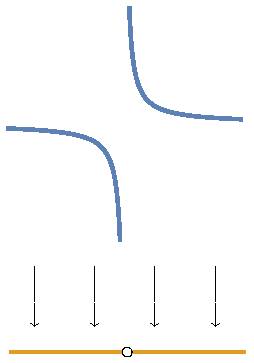
\includegraphics[width=\linewidth]{figures/affine-hyperbola-open-projection.pdf}
}
换一种方式说明仿射簇和射影簇的区别. 回顾在第~\ref{sec:affine-varieties-revisited}~节, 我们特意重新定义\textquotedbl{}仿射簇\textquotedbl{}, 让它不仅指 $\mathbb{A}^{n}$ 的闭子集, 而且指同构于这类子集的拟射影簇. 不过, 可以放心地把\textquotedbl{}射影簇\textquotedbl{}简单定义为 $\mathbb{P}^{n}$ 的一个闭子集, 因为这个概念已经在同构下保持. 的确, 由 Theorem~\ref{thm:regular-images-of-projective-varieties-are-closed} 可推出 (Corollary~\ref{cor:projectivity-invariant-under-quasiprojective-isomorphism}), 若拟射影簇 $X\subseteq\mathbb{P}^{n}$ 同构于另一个射影空间的闭子集, 则 $X$ 在 $\mathbb{P}^{n}$ 中也必是闭的.

本节还将用 Corollary~\ref{cor:regular-functions-on-irreducible-projective-varieties-are-constant} 描述仿射簇和射影簇的另一项区别. 与仿射簇上丰富的多项式函数相比, 不可约射影簇上没有非常值的正则函数. 关键是把 $X$ 上的正则函数看成正则映射 $F:X\to\mathbb{A}^{1}$, 并利用 $\mathbb{A}^{1}$ 的闭子集只有 $\mathbb{A}^{1}$ 本身和有限点集这一事实. $X$ 的不可约性和射影性意味着, 在这些可能性中, $F(X)$ 必是单个点.

有了这些动机, 开始证明 Theorem~\ref{thm:regular-images-of-projective-varieties-are-closed}. 由 Exercise~\ref{ex:image-of-map-is-projection-of-graph}, 从略有不同的角度来看, 正则映射 $F:X\to Y$ 的像 $F(X)$ 满足 $F(X)=\pi(\Gamma_{F})$, 其中 $\Gamma_{F}\subseteq X\times Y$ 是 $F$ 的图像, $\pi$ 是到第二个因子的投影:
\[
  \begin{aligned}
    \pi:X\times Y&\to Y\\
    \pi(x,y)&=y.
  \end{aligned}
\]
由于 $\Gamma_{F}$ 在 $X\times Y$ 中闭 (Proposition~\ref{prop:graphs-of-quasiprojective-regular-maps-are-closed}), 只需证明以下结论.

\begin{Lemma}{从射影簇出发的投影是闭映射}\leavevmode\label{lem:projection-from-projective-factor-is-closed}
若 $X\subseteq\mathbb{P}^{m}$ 闭, $Y\subseteq\mathbb{P}^{n}$ 为拟射影簇, 则投影 $\pi:X\times Y\to Y$ 将 $X\times Y$ 的闭集映为 $Y$ 的闭集.
\end{Lemma}
\begin{Proof}
这个证明颇为复杂, 先作一系列归约. 首先归约到 $X=\mathbb{P}^{m}$ 的情形, 再归约到 $Y$ 为仿射簇的情形, 最后归约到 $Y$ 为 $\mathbb{A}^{n}$ 的情形. 然后在 $X\times Y=\mathbb{P}^{m}\times\mathbb{A}^{n}$ 的情形证明结果.

\textbf{(归约到 $X=\mathbb{P}^{m}$)} 假设引理在 $X=\mathbb{P}^{m}$ 时成立, 令 $X\subseteq\mathbb{P}^{m}$ 闭, 并设 $Z\subseteq X\times Y$ 闭. 由于 $X$ 在 $\mathbb{P}^{m}$ 中闭, $X\times Y$ 在 $\mathbb{P}^{m}\times Y$ 中闭 (Exercise~\ref{ex:product-of-closed-quasiprojective-subvarieties-is-closed}), 因此闭包含
\[
  Z\subseteq X\times Y\subseteq\mathbb{P}^{m}\times Y
\]
表明 $Z$ 在 $\mathbb{P}^{m}\times Y$ 中闭. 若 $\pi:X\times Y\to Y$ 与 $\overline{\pi}:\mathbb{P}^{m}\times Y\to Y$ 分别表示相应的投影, 则由假设 $\overline{\pi}(Z)$ 在 $Y$ 中闭. 但 $\pi(Z)=\overline{\pi}(Z)$, 所以 $\pi(Z)$ 在 $Y$ 中也闭.

这样, $X=\mathbb{P}^{m}$ 的特例蕴含引理的一般情形, 故以下假设 $X=\mathbb{P}^{m}$.

\textbf{(归约到 $Y$ 为仿射簇)} 假设引理在 $Y$ 为仿射簇时成立, 令 $Y$ 为任一拟射影簇. 设 $Z\subseteq\mathbb{P}^{m}\times Y$ 闭. 由于拟射影簇是局部仿射的 (Theorem~\ref{thm:quasiprojective-varieties-have-finite-affine-open-covers}), 对每个 $p\in Y$, 都存在包含 $p$ 的仿射开集 $Y_{p}\subseteq Y$. 将闭集 $Z\subseteq\mathbb{P}^{m}\times Y$ 与 $\mathbb{P}^{m}\times Y_{p}$ 相交, 可见
\[
  Z\cap(\mathbb{P}^{m}\times Y_{p})\subseteq\mathbb{P}^{m}\times Y_{p}
\]
对每个 $p$ 都在 $\mathbb{P}^{m}\times Y_{p}$ 中闭. 因此, 由假设, 在投影 $\pi_{p}:\mathbb{P}^{m}\times Y_{p}\to Y_{p}$ 下的像
\[
  \pi_{p}(Z\cap(\mathbb{P}^{m}\times Y_{p}))\subseteq Y_{p}
\]
在 $Y_{p}$ 中闭. 但 $\pi(Z)\cap Y_{p}=\pi_{p}(Z\cap(\mathbb{P}^{m}\times Y_{p}))$, 所以已证明 $\pi(Z)\cap Y_{p}$ 在 $Y_{p}$ 中闭. 因为这对每个 $p\in Y$ 都成立, 可见 $\pi(Z)$ 在 $Y$ 中局部闭, 因而由 Lemma~\ref{lem:closedness-is-local}, 它在 $Y$ 中闭.

这样, $Y$ 为仿射簇的特例蕴含引理的一般情形, 故以下还假设 $Y$ 为仿射簇.

\textbf{(归约到 $Y=\mathbb{A}^{n}$)} 最后假设引理在 $Y=\mathbb{A}^{n}$ 时成立, 令 $Y\subseteq\mathbb{A}^{n}$ 闭. 设 $Z\subseteq\mathbb{P}^{m}\times Y$ 闭, 注意 $Z$ 作为 $\mathbb{P}^{m}\times\mathbb{A}^{n}$ 的子集也闭. 令 $\pi:\mathbb{P}^{m}\times Y\to Y$ 和 $\overline{\pi}:\mathbb{P}^{m}\times\mathbb{A}^{n}\to\mathbb{A}^{n}$ 分别表示相应的投影. 由于 $\pi(Z)=\overline{\pi}(Z)$, 且由假设 $\overline{\pi}(Z)$ 在 $\mathbb{A}^{n}$ 中闭, 所以 $\pi(Z)$ 在 $Y$ 中闭.

这样, 已将整个引理归约到 $X=\mathbb{P}^{m}$ 和 $Y=\mathbb{A}^{n}$ 的特例. 现在着手证明这一特例. 不过要提醒读者, 下面的论证相当繁复. 在读证明之前或一边读证明一边做下面的 Example~\ref{ex:projecting-closed-set-by-coefficient-matrix}, 可能有助于理解其策略和记号.

\textbf{($X=\mathbb{P}^{m}$ 且 $Y=\mathbb{A}^{n}$ 时的证明)} 设 $Z\subseteq\mathbb{P}^{m}\times\mathbb{A}^{n}$ 闭, 写成
\[
  Z=\mathcal{V}(f_{1},\ldots,f_{\ell}),
\]
其中 $f_{1},\ldots,f_{\ell}\in K[x_{0},\ldots,x_{m},y_{1},\ldots,y_{n}]$. 可以假定每个 $f_{k}$ 关于 $x$ 变量齐次, 并令 $d_{k}$ 表示 $f_{k}$ 关于 $x$ 变量的次数. 注意
\begin{equation}\label{eq:projection-image-nonempty-fibre}
  \pi(Z)=\{b\in\mathbb{A}^{n}\mid\pi^{-1}(b)\cap Z\ne\varnothing\}.
\end{equation}
其余论证的核心是分析条件 $\pi^{-1}(b)\cap Z\ne\varnothing$.

给定 $b=(b_{1},\ldots,b_{n})\in\mathbb{A}^{n}$, 对每个 $k=1,\ldots,\ell$ 定义
\begin{equation}\label{eq:specialize-defining-polynomial-at-affine-point}
  f_{k}^{b}(x_{0},\ldots,x_{m})
  =f_{k}(x_{0},\ldots,x_{m},b_{1},\ldots,b_{n})\in K[x_{0},\ldots,x_{m}].
\end{equation}
自然地将集合
\[
  \pi^{-1}(b)\cap Z
  =\{(a,b)\in\mathbb{P}^{m}\times\{b\}\mid f_{k}^{b}(a)=0\text{ 对所有 }k=1,\ldots,\ell\}
\]
与消没集 $\mathcal{V}(f_{1}^{b},\ldots,f_{\ell}^{b})\subseteq\mathbb{P}^{m}$ 等同. 这样, $\pi^{-1}(b)\cap Z$ 为空的刻画是
\[
  \pi^{-1}(b)\cap Z=\varnothing
  \iff \mathcal{V}(f_{1}^{b},\ldots,f_{\ell}^{b})=\varnothing\subseteq\mathbb{P}^{m}.
\]
由射影零点定理, 条件 $\mathcal{V}(f_{1}^{b},\ldots,f_{\ell}^{b})=\varnothing$ 等价于存在某个 $r\ge0$, 使每个 $r$ 次单项式 $x^{\alpha}$ 都属于 $\langle f_{1}^{b},\ldots,f_{\ell}^{b}\rangle$ (Exercise~\ref{ex:empty-projective-variety-criterion-by-degree}). 为方便起见, 令 $M_{r}$ 为 $x_{0},\ldots,x_{m}$ 的 $r$ 次单项式的指标集, 因而每个 $\alpha\in M_{r}$ 对应一个 $r$ 次单项式 $x^{\alpha}$. 于是, $\pi^{-1}(b)\cap Z=\varnothing$, 当且仅当存在 $r\ge0$, 使对每个 $\alpha\in M_{r}$ 都有
\begin{equation}\label{eq:degree-r-monomial-in-specialized-ideal}
  x^{\alpha}=\sum_{k=1}^{\ell}g_{k}f_{k}^{b},
\end{equation}
其中 $g_{1},\ldots,g_{\ell}\in K[x_{0},\ldots,x_{m}]$. 可用单项式 $x^{\beta}$ 写出 $g_{k}=\sum_{\beta}a_{k,\beta}x^{\beta}$, 从而 \eqref{eq:degree-r-monomial-in-specialized-ideal} 等价于存在 $a_{k,\beta}\in K$ 使
\begin{equation}\label{eq:monomial-expansion-of-specialized-ideal-membership}
  x^{\alpha}=\sum_{k=1}^{\ell}\sum_{\beta}a_{k,\beta}x^{\beta}f_{k}^{b}.
\end{equation}
由于 $\alpha\in M_{r}$ 且 $f_{k}^{b}$ 是 $d_{k}$ 次齐次多项式, 可以假定 \eqref{eq:monomial-expansion-of-specialized-ideal-membership} 的第 $k$ 个加项中出现的每个 $\beta$ 都在 $M_{r-d_{k}}$ 中, 因为所有其他项之和必为零. 对每个 $k\in\{1,\ldots,\ell\}$ 及每个 $\beta\in M_{r-d_{k}}$, 现在把 $x^{\beta}f_{k}^{b}$ 写成单项式的线性组合:
\begin{equation}\label{eq:coefficient-matrix-row-of-specialized-monomial-multiple}
  x^{\beta}f_{k}^{b}=\sum_{\alpha}c_{(k,\beta),\alpha}^{b}x^{\alpha},
\end{equation}
并把这些线性组合的系数排列成矩阵
\[
  C_{r}^{b}=\bigl(c_{(k,\beta),\alpha}^{b}\bigr).
\]
注意 $C_{r}^{b}$ 的列由 $M_{r}$ 编号, 行则由 $(k,\beta)$ 编号, 其中 $\beta\in M_{r-d_{k}}$.

注意, $C_{r}^{b}$ 中由 $(k,\beta)$ 编号的行记录了 $x^{\beta}f_{k}^{b}$ 作为 $\{x^{\alpha}\mid\alpha\in M_{r}\}$ 的线性组合的系数. 因此, 对每个 $\alpha\in M_{r}$ 都存在 \eqref{eq:monomial-expansion-of-specialized-ideal-membership} 中的表示, 等价于标准基向量都在 $C_{r}^{b}$ 的行张成的空间内. 这又等价于 $C_{r}^{b}$ 的秩为 $|M_{r}|$ (即 $C_{r}^{b}$ 的列数). 总结起来, 已证明
\[
  \pi^{-1}(b)\cap Z=\varnothing
  \iff\text{存在 }r\ge0\text{ 使 }\operatorname{rk}(C_{r}^{b})=|M_{r}|.
\]
将以上条件取否定, 得
\[
  \pi^{-1}(b)\cap Z\ne\varnothing
  \iff\text{对每个 }r\ge0,\ \operatorname{rk}(C_{r}^{b})<|M_{r}|.
\]
由此可知, $\pi^{-1}(b)\cap Z\ne\varnothing$ 当且仅当对每个 $r\ge0$, $C_{r}^{b}$ 的所有 $|M_{r}|\times|M_{r}|$ 子式均消没. 这些子式是 $C_{r}^{b}$ 各项的多项式表达式, 而由 \eqref{eq:specialize-defining-polynomial-at-affine-point} 和 \eqref{eq:coefficient-matrix-row-of-specialized-monomial-multiple} 中的定义可知, $C_{r}^{b}$ 的每一项都是 $b_{1},\ldots,b_{n}$ 的多项式表达式. 因此, 所有满足 $\pi^{-1}(b)\cap Z\ne\varnothing$ 的 $b\in\mathbb{A}^{n}$ 构成 $\mathbb{A}^{n}$ 的一个闭子集. 再由 \eqref{eq:projection-image-nonempty-fibre} 得 $\pi(Z)$ 闭, 证明完成.
\end{Proof}

在下一例中, 我们具体说明 Lemma~\ref{lem:projection-from-projective-factor-is-closed} 的证明中用到的一些记号.

\begin{Example}{闭集的投影}\leavevmode\label{ex:projecting-closed-set-by-coefficient-matrix}
为了说明 Lemma~\ref{lem:projection-from-projective-factor-is-closed} 的证明策略, 考察闭子集
\[
  Z=\mathcal{V}(x_{0}+y_{1}x_{1},x_{1}^{2}+y_{2}x_{0}x_{1})
  \subseteq\mathbb{P}^{1}\times\mathbb{A}^{2}
\]
及其在投影 $\pi:\mathbb{P}^{1}\times\mathbb{A}^{2}\to\mathbb{A}^{2}$ 下的像. 首先注意, 例如 $(1,0)\notin\pi(Z)$, 因为在 $Z$ 的定义方程中取 $y_{1}=1$ 和 $y_{2}=0$, 得
\[
  \pi^{-1}(1,0)\cap Z
  =\left\{[a_{0}:a_{1}]\in\mathbb{P}^{1}\ \middle|\
    \substack{a_{0}+a_{1}=0,\\ a_{1}^{2}=0}\right\}=\varnothing.
\]
另一方面, 例如 $(1,1)\in\pi(Z)$, 因为在 $Z$ 的定义方程中取 $y_{1}=y_{2}=1$, 得
\[
  \pi^{-1}(1,1)\cap Z
  =\left\{[a_{0}:a_{1}]\in\mathbb{P}^{1}\ \middle|\
    \substack{a_{0}+a_{1}=0,\\a_{1}^{2}+a_{0}a_{1}=0}\right\}=\{[1:-1]\}.
\]

一般来说, Lemma~\ref{lem:projection-from-projective-factor-is-closed} 的证明表明, $b=(b_{1},b_{2})\in\pi(Z)$ 当且仅当对每个 $r\ge0$, 矩阵 $C_{r}^{b}$ 的所有 $|M_{r}|\times|M_{r}|$ 子式都为零. 为了理解这一叙述, 特别是理解这些记号, 我们显式计算 $r=3$ 时的矩阵.

为对一般的 $b=(b_{1},b_{2})$ 计算矩阵 $C_{3}^{b}$, 首先考察多项式
\[
  f_{1}^{b}=x_{0}+b_{1}x_{1}\qquad\text{和}\qquad f_{2}^{b}=x_{1}^{2}+b_{2}x_{0}x_{1}.
\]
将这两个多项式各自乘以所有能使乘积关于 $x$ 变量为三次的 $x_{0},x_{1}$ 的单项式, 并记录结果中单项式 $x_{0}^{3}$, $x_{0}^{2}x_{1}$, $x_{0}x_{1}^{2}$ 和 $x_{1}^{3}$ 的系数, 得到
\[
  \begin{aligned}
  f_{1}^{b}\cdot x_{0}^{2}&=\boxed{1}\cdot x_{0}^{3}+\boxed{b_{1}}\cdot x_{0}^{2}x_{1}
        +\boxed{0}\cdot x_{0}x_{1}^{2}+\boxed{0}\cdot x_{1}^{3}\\
  f_{1}^{b}\cdot x_{0}x_{1}&=\boxed{0}\cdot x_{0}^{3}+\boxed{1}\cdot x_{0}^{2}x_{1}
        +\boxed{b_{1}}\cdot x_{0}x_{1}^{2}+\boxed{0}\cdot x_{1}^{3}\\
  f_{1}^{b}\cdot x_{1}^{2}&=\boxed{0}\cdot x_{0}^{3}+\boxed{0}\cdot x_{0}^{2}x_{1}
        +\boxed{1}\cdot x_{0}x_{1}^{2}+\boxed{b_{1}}\cdot x_{1}^{3}\\
  f_{2}^{b}\cdot x_{0}&=\boxed{0}\cdot x_{0}^{3}+\boxed{b_{2}}\cdot x_{0}^{2}x_{1}
        +\boxed{1}\cdot x_{0}x_{1}^{2}+\boxed{0}\cdot x_{1}^{3}\\
  f_{2}^{b}\cdot x_{1}&=\boxed{0}\cdot x_{0}^{3}+\boxed{0}\cdot x_{0}^{2}x_{1}
        +\boxed{b_{2}}\cdot x_{0}x_{1}^{2}+\boxed{1}\cdot x_{1}^{3}.
  \end{aligned}
\]
则 $C_{3}^{b}$ 是由方框中的各项构成的 $5\times4$ 矩阵, 这矩阵的 $4\times4$ 子式消没是 $b$ 属于 $\pi(Z)$ 的必要条件. 其中一个子式是删去 $C_{3}^{b}$ 的第四行所得矩阵的行列式, 读者可以核对它等于
\[
  1-b_{1}b_{2}.
\]
特别地, 元素 $b=(b_{1},b_{2})\in\pi(Z)$ 必须满足 $b_{1}b_{2}=1$, 这和我们算出的 $(1,0)\notin\pi(Z)$ 但 $(1,1)\in\pi(Z)$ 一致.

由 $C_{3}^{b}$ 的其他子式以及其他 $r\ge1$ 的 $C_{r}^{b}$ 的子式消没, 还得到关于 $b_{1},b_{2}$ 的更多条件. 不过, 实际上它们都由单一条件 $b_{1}b_{2}=1$ 蕴含. 可直接由 $\pi(Z)$ 的定义核验这一点: 它由所有满足
\[
  a_{0}+b_{1}a_{1}=0=a_{1}^{2}+b_{2}a_{0}a_{1}
  \qquad\text{对某个 }[a_{0}:a_{1}]\in\mathbb{P}^{1}
\]
的点 $(b_{1},b_{2})\in\mathbb{A}^{2}$ 组成. 这个方程组很容易解得 $b_{1}b_{2}=1$. 因此, 无论用这一直接计算, 还是用上面说明的子式方法, 都得到 $\pi(Z)$ 确实是一个闭集: $\pi(Z)=\mathcal{V}(y_{1}y_{2}-1)\subseteq\mathbb{A}^{2}$.
\end{Example}

Theorem~\ref{thm:regular-images-of-projective-varieties-are-closed} 的证明现在可由 Lemma~\ref{lem:projection-from-projective-factor-is-closed} 很快得到.
\begingroup
\renewcommand{\AJProofBegin}{%
  \par\addvspace{\topsep}\noindent
  {\sffamily\bfseries\CJKfamily{pffont}Proof of Theorem~\ref{thm:regular-images-of-projective-varieties-are-closed}}\enspace\ignorespaces
}
\begin{Proof}
由于 $F(X)=\pi(\Gamma_{F})$, 且由 Proposition~\ref{prop:graphs-of-quasiprojective-regular-maps-are-closed} 知 $\Gamma_{F}\subseteq X\times Y$ 在 $X\times Y$ 中闭, 由 Lemma~\ref{lem:projection-from-projective-factor-is-closed} 可知 $F(X)$ 在 $Y$ 中闭.
\end{Proof}
\endgroup

现在验证本节开头提到的 Theorem~\ref{thm:regular-images-of-projective-varieties-are-closed} 的两个重要推论.

\begin{Corollary}{在射影空间中闭是内在性质}\leavevmode\label{cor:projectivity-invariant-under-quasiprojective-isomorphism}
若 $X\subseteq\mathbb{P}^{m}$ 和 $Y\subseteq\mathbb{P}^{n}$ 是同构的拟射影簇, 则 $X$ 在 $\mathbb{P}^{m}$ 中闭, 当且仅当 $Y$ 在 $\mathbb{P}^{n}$ 中闭.
\end{Corollary}
\begin{Proof}
设 $X$ 在 $\mathbb{P}^{m}$ 中闭, 且 $F:X\to Y$ 为同构. 可以把 $F$ 视为从 $X$ 到 $\mathbb{P}^{n}$ 的正则映射, 由 Theorem~\ref{thm:regular-images-of-projective-varieties-are-closed} 可知 $F(X)$ 在 $\mathbb{P}^{n}$ 中闭. 但因 $F$ 是同构, $F(X)=Y$, 所以 $Y$ 在 $\mathbb{P}^{n}$ 中闭. 双向陈述由对称性得到.
\end{Proof}

\begin{Corollary}{射影簇上的正则函数}\leavevmode\label{cor:regular-functions-on-irreducible-projective-varieties-are-constant}
若 $X$ 为不可约射影簇, 则 $X$ 上每个正则函数都为常值. 换句话说, $K[X]=K$.
\end{Corollary}
\begin{Proof}
正则函数 $F:X\to K$ 与正则映射 $F:X\to\mathbb{A}^{1}$ 相同, 所以 Theorem~\ref{thm:regular-images-of-projective-varieties-are-closed} 蕴含 $F(X)\subseteq\mathbb{A}^{1}$ 是闭的. $\mathbb{A}^{1}$ 的非空闭子集只有整个 $\mathbb{A}^{1}$ 和有限点集. 不可能有 $F(X)=\mathbb{A}^{1}$, 因为如果如此, 将 $F$ 与包含映射 $j_{0}:\mathbb{A}^{1}\to\mathbb{P}^{1}$ 复合会给出正则映射 $X\to\mathbb{P}^{1}$, 其像等于 $\mathbb{A}^{1}\subseteq\mathbb{P}^{1}$, 而这个像并不闭.

因此, $F$ 的像必为有限点集 $a_{1},\ldots,a_{\ell}\in\mathbb{A}^{1}$, 意味着
\[
  X=F^{-1}(a_{1})\sqcup\cdots\sqcup F^{-1}(a_{\ell}).
\]
这个不交并中的每个集合都在 $X$ 中闭 (Theorem~\ref{thm:regular-maps-are-zariski-continuous}), 所以 $X$ 的不可约性蕴含必有 $\ell=1$. 换句话说, $F(X)$ 只由一个元素组成, 所以 $F$ 是常值函数.
\end{Proof}

本节最后回到一个熟悉的例子.

\begin{Example}{$\mathbb{A}^{2}\setminus\{(0,0)\}$ 不是射影簇}\leavevmode\label{ex:punctured-affine-plane-is-not-projective}
如在 Example~\ref{ex:punctured-affine-plane-is-not-affine} 中看到的, 拟射影簇 $\mathbb{A}^{2}\setminus\{(0,0)\}$ 不同构于仿射簇. 现在也可以验证它不同构于射影簇. 我们给出两种论证, 分别依赖刚证明的关于射影簇的两个推论之一.

第一种论证基于 $\mathbb{A}^{2}\setminus\{(0,0)\}\subseteq\mathbb{P}^{2}$ 不闭这一事实. 的确, $\mathbb{A}^{2}\setminus\{(0,0)\}$ 是 $\mathbb{P}^{2}$ 的非空开子集, 从而稠密. 因此它只有在等于整个 $\mathbb{P}^{2}$ 时才可能闭, 但它并不等于整个 $\mathbb{P}^{2}$. 由于 $\mathbb{A}^{2}\setminus\{(0,0)\}$ 在 $\mathbb{P}^{2}$ 中不闭, Corollary~\ref{cor:projectivity-invariant-under-quasiprojective-isomorphism} 蕴含它不同构于射影簇.

第二种论证基于 Example~\ref{ex:punctured-affine-plane-is-not-affine} 中的观察:
\[
  K[\mathbb{A}^{2}\setminus\{(0,0)\}]=K[x,y].
\]
由于 $\mathbb{A}^{2}\setminus\{(0,0)\}$ 的正则函数环并不只是常值函数 $K$, 由 Corollary~\ref{cor:regular-functions-on-irreducible-projective-varieties-are-constant} 可知 $\mathbb{A}^{2}\setminus\{(0,0)\}$ 不可能同构于射影簇.
\end{Example}

本章开始熟悉拟射影簇的理论. 重要的是, 现在已经精确说明仿射簇和射影簇如何处在这一更一般的框架之中. 在下一章, 即本书最后一章, 我们转向拟射影簇的若干关键性质, 如维数和光滑性. 在本章工作的基础上, 我们会看到, 利用拟射影簇的局部仿射性质, 不需太多额外工作, 就能直接从仿射情形引入这些性质的基本特征.

\BookExerciseHeading
\begin{BookExercises}
  \item\label{ex:image-of-map-is-projection-of-graph} 令 $F:X\to Y$ 为集合之间的函数, $\Gamma_{F}\subseteq X\times Y$ 为 $F$ 的图像. 证明 $F(X)=\pi(\Gamma_{F})$, 其中 $\pi:X\times Y\to Y$ 为投影映射.
  \item\label{ex:coefficient-matrix-for-quadratic-multiples-in-projection-example} 令 $Z\subseteq\mathbb{P}^{1}\times\mathbb{A}^{2}$ 如 Example~\ref{ex:projecting-closed-set-by-coefficient-matrix} 所示, 计算矩阵 $C_{2}^{b}$. 这个矩阵的子式消没给出 $b\in\pi(Z)$ 的哪些条件? 验证当 $b_{1}b_{2}=1$ 时这些条件都满足, 如 Example~\ref{ex:projecting-closed-set-by-coefficient-matrix} 所断言.
  \item\label{ex:projection-of-common-root-of-two-linear-forms} 令 $Z=\mathcal{V}(x_{0}+y_{1}x_{1},x_{0}+y_{2}x_{1})\subseteq\mathbb{P}^{1}\times\mathbb{A}^{2}$, 令 $\pi:\mathbb{P}^{1}\times\mathbb{A}^{2}\to\mathbb{A}^{2}$ 表示投影.
  \begin{enumerate}
    \item 直接计算像 $\pi(Z)$.
    \item 计算矩阵 $C_{1}^{b}$ 和 $C_{2}^{b}$, 并确认当 $b\in\pi(Z)$ 时, 它们的所有最大阶子式均消没.
  \end{enumerate}
  \item\label{ex:regular-map-from-projective-to-affine-is-constant} 证明从不可约射影簇到仿射簇的每个正则映射都是常值的.
  \item\label{ex:projective-line-times-affine-line-is-neither-affine-nor-projective} 证明 $\mathbb{P}^{1}\times\mathbb{A}^{1}$ 既不 (同构于) 仿射簇, 也不 (同构于) 射影簇.
  \item\label{ex:punctured-projective-plane-is-neither-affine-nor-projective} 证明 $\mathbb{P}^{2}\setminus\{[1:0:0]\}$ 既不 (同构于) 仿射簇, 也不 (同构于) 射影簇.
  \item\label{ex:projective-line-endomorphism-constant-or-surjective} 证明每个正则映射 $\mathbb{P}^{1}\to\mathbb{P}^{1}$ 或为常值, 或为满射.
\end{BookExercises}

\chapter{进阶专题}\label{chap:rational-maps}

\noindent\textbf{第 \thechapter{} 章学习目标}
\begin{itemize}
  \item 描述拟射影簇上的有理函数和拟射影簇之间的有理映射.
  \item 定义拟射影簇的维数, 切空间和光滑性, 并引入仿射簇理论的关键结果.
  \item 研究 $\mathbb{A}^{n}$ 在一点的爆破, 通过例子探索它如何用于消解奇点.
  \item 计算正则映射的纤维的维数.
  \item 利用 Grassmann 簇与维数理论研究 $\mathbb{P}^{3}$ 中曲面上的直线.
  \item 数出光滑三次曲面上的直线.
\end{itemize}

在本书最后一章, 我们讨论若干进阶专题, 将此前关于仿射簇, 射影簇和拟射影簇的发展联系起来. 在前三节, 进一步发展仿射情形和拟射影情形的平行关系, 把维数和光滑性的概念推广到拟射影情形. 在某种意义上, 这些推广几乎不需要额外工作: 维数和光滑性都是局部性质, 而每个拟射影簇都是局部仿射的, 因此可以把对仿射簇的维数和光滑性的理解直接引入拟射影情形.

第四节探索\textquotedbl{}爆破\textquotedbl{}的概念. 这一构造将簇中的一点替换为参数化该点切方向的射影空间. 如将从例子中看到的, 爆破的一个关键用途是消解簇的奇点. 本节的重要启示是, 即使起初只关心仿射簇, 消解奇点的尝试也会自然地把我们带到拟射影情形.

接着转向关于正则映射的一个关键定理, 它是秩-零化度定理的大幅推广, 根据定义域和陪域的维数描述正则映射的\textquotedbl{}纤维\textquotedbl{}的维数. 如将看到的, 该结果的一个几何应用是: $\mathbb{P}^{3}$ 中由次数至多为三的齐次多项式定义的每张曲面都包含至少一条直线.

我们最终在最后一节给出代数几何最著名的经典结果之一: $\mathbb{P}^{3}$ 中每张光滑三次曲面恰好包含 27 条直线. 引人注目的是, 不论是直线的条数, 还是哪些直线两两相交的组合结构, 都不依赖于基域或光滑三次曲面的定义方程. 这一经典结果让我们得以一瞥其中丰富而优美的结构, 读者在继续研究代数几何时会愈加熟悉它们.

\par\smallskip
{\footnotesize
\noindent\textcopyright{} The Author(s) 2025\par
\noindent E. Clader, D. Ross, \emph{Beginning in Algebraic Geometry}, Undergraduate Texts in Mathematics,
\href{https://doi.org/10.1007/978-3-031-88819-9_13}{\nolinkurl{https://doi.org/10.1007/978-3-031-88819-9_13}}.\par}

\section{有理函数}\label{sec:rational-maps-between-varieties}

为在下一节定义拟射影簇的维数作准备, 本节引入有理函数. 在仿射簇的情形, $X$ 上的有理函数定义为 $\operatorname{Frac}(K[X])$ 的元素, 即 $X$ 上多项式函数的商. 当 $X\subseteq\mathbb{P}^{n}$ 为拟射影簇时, 仍然考虑多项式的商, 但新的关键之处在于: 同次数的两个齐次多项式 $f,g\in K[x_{0},\ldots,x_{n}]$ 的商, 现在可以看作在开集 $X\setminus\mathcal{V}(g)$ 上定义一个正则函数. 基于这个观察, 我们用开集上的正则函数定义拟射影簇上的有理函数.

\begin{Definition}{拟射影簇上的有理函数}\leavevmode\label{def:rational-function-on-quasiprojective-variety}
设 $X$ 为拟射影簇. $X$ 上的一个\emph{有理函数}是数对 $(U,F)$ 的一个等价类, 其中 $U\subseteq X$ 为 $X$ 的稠密开子集, $F$ 为 $U$ 上的正则函数, 等价关系为
\[
  (U,F)\sim(V,G)\iff F(a)=G(a)\quad\forall a\in U\cap V.
\]
\end{Definition}

直观地说, $X$ 上的有理函数是\textquotedbl{}几乎处处\textquotedbl{}有定义的正则函数. 这与 $1/x$ 这样的商是 $\mathbb{A}^{1}\setminus\{0\}$ 上的正则函数大致相同, 而这个集合是 $\mathbb{A}^{1}$ 的\textquotedbl{}几乎全部\textquotedbl{}. 应当核对 Definition~\ref{def:rational-function-on-quasiprojective-variety} 中的关系是不是等价关系 (Exercise~\ref{ex:dense-open-rational-function-equivalence-relation}). 这里的关键是定义域稠密, 而不仅是开, 从而一个有理函数的两个代表的定义域必相交于稠密开子集. 引入等价关系的动机很简单: 一个有理函数的不同代表可能有不同的定义域, 但如果它们\textquotedbl{}几乎处处\textquotedbl{}相等, 我们就想把它们视为等价. 下面的例子说明这一等价概念.

\begin{Example}{$\mathbb{P}^{1}$ 上的有理函数}\leavevmode\label{ex:equivalent-rational-functions-on-projective-line}
令 $U=\mathbb{P}^{1}\setminus\{[1:0]\}$, $V=\mathbb{P}^{1}\setminus\{[1:0],[0:1]\}$, 考察由下式定义的正则函数 $F\in K[U]$ 和 $G\in K[V]$:
\[
  F([a:b])=\frac{a}{b}\qquad\text{和}\qquad G([a:b])=\frac{a^{2}}{ba}.
\]
注意 $U,V$ 都是 $\mathbb{P}^{1}$ 的稠密开子集, 因而 $(U,F)$ 和 $(V,G)$ 都给出 $\mathbb{P}^{1}$ 上的有理函数. 再者, 由于 $F$ 和 $G$ 在 $U\cap V$ 上相等, 可知 $(U,F)\sim(V,G)$. 直观地说, $F$ 和 $G$ 定义同一个有理函数, 只是因为定义 $G$ 的商约分后就是定义 $F$ 的商.
\end{Example}

$X$ 上的有理函数一般记为 $F:X\mathrel{\rightdasharrow} K$, 其中虚线箭头表示 $F$ 可能未在整个 $X$ 上定义. 有理函数 $F:X\mathrel{\rightdasharrow} K$ 的\emph{定义域}是它的所有代表的定义域的并. 由于稠密开子集对并封闭, 有理函数的定义域是 $X$ 的稠密开子集. 再者, 由正则函数的局部性质, 有理函数 $F:X\mathrel{\rightdasharrow} K$ 在其定义域上正则. 因此可以把有理函数的定义域看成它正则的最大集合.

和正则函数的集合一样, 有理函数的集合自然构成一个 $K$-代数 (Exercise~\ref{ex:rational-functions-form-algebra}), 从而得到以下定义.

\begin{Definition}{有理函数环}\leavevmode\label{def:ring-of-rational-functions}
令 $X$ 为拟射影簇. $X$ 上的\emph{有理函数环}记为 $K(X)$, 是所有有理函数 $F:X\mathrel{\rightdasharrow} K$ 构成的 $K$-代数.
\end{Definition}

由于拟射影簇的同构把开集及其上的正则函数环一一对应起来 (Corollary~\ref{cor:characterize-quasiprojective-isomorphisms-by-local-rings-of-functions}), 可知拟射影簇上的正则函数环是内在的 (Exercise~\ref{ex:rational-function-rings-invariant-under-isomorphism}).

下面看几个正则函数环的具体例子.

\begin{Example}{$K(\mathbb{P}^{n})=K(x_{1},\ldots,x_{n})$}\leavevmode\label{ex:rational-function-field-of-projective-space}
首先论证 $\mathbb{P}^{n}$ 上的有理函数都可用 $K[x_{0},\ldots,x_{n}]$ 中同次数的齐次多项式的商表示. 这样的商显然定义了 $\mathbb{P}^{n}$ 上的有理函数: 给定同次数的齐次多项式 $f,g\in K[x_{0},\ldots,x_{n}]$, $f/g$ 在开集 $U=\mathbb{P}^{n}\setminus\mathcal{V}(g)$ 上定义一个正则函数, 该开集稠密, 因为 $\mathbb{P}^{n}$ 不可约. 反过来, 给定 $\mathbb{P}^{n}$ 上由开子集 $U\subseteq\mathbb{P}^{n}$ 上的正则函数 $F:U\to K$ 表示的任一有理函数, Lemma~\ref{lem:regular-functions-on-projective-open-subsets-are-global-quotients} 表明, 存在同次数的齐次多项式 $f,g\in K[x_{0},\ldots,x_{n}]$, 使 $\mathcal{V}(g)\cap U=\varnothing$, 且在 $U$ 上有 $F=f/g$. 由此得
\[
  (U,F)\sim(\mathbb{P}^{n}\setminus\mathcal{V}(g),f/g),
\]
这说明 $\mathbb{P}^{n}$ 上的任意有理函数都能表示为同次数的齐次多项式的商, 如所断言.

稍加思考可知, 两个商 $f_{1}/g_{1}$ 和 $f_{2}/g_{2}$ 定义同一个 $\mathbb{P}^{n}$ 上的有理函数, 当且仅当 $f_{1}g_{2}-f_{2}g_{1}=0$. 这与定义 $K(x_{0},\ldots,x_{n})=\operatorname{Frac}(K[x_{0},\ldots,x_{n}])$ 中元素的关系相同. 换句话说, 可以把 $K(\mathbb{P}^{n})$ 与 $K(x_{0},\ldots,x_{n})$ 的一个子环等同, 该子环由分子与分母都是同次数齐次多项式的商组成. 关于 $x_{0}$ 去齐次化后, 得到 $K(\mathbb{P}^{n})=K(x_{1},\ldots,x_{n})$.
\end{Example}

\begin{Example}{$\mathcal{V}(xy)\subseteq\mathbb{P}^{2}$ 上的有理函数}\leavevmode\label{ex:rational-functions-on-union-of-projective-lines}
令 $X$ 为可约簇 $\mathcal{V}(xy)\subseteq\mathbb{P}^{2}$, 由两个分支 $\mathcal{V}(x)$ 和 $\mathcal{V}(y)$ 组成. 定义有理函数 $F:X\mathrel{\rightdasharrow} K$ 和 $G:X\mathrel{\rightdasharrow} K$ 为
\[
  F([a:b:c])=a/c\qquad\text{和}\qquad G([a:b:c])=b/c,
\]
它们都定义在稠密开集 $U=X\setminus\{[1:0:0],[0:1:0]\}$ 上. 因为 $F,G$ 都不在其定义域上消没, 它们在 $K(X)$ 中都不为零. 但乘积 $F\cdot G$ 在 $U$ 上消没. 由此可见, $X$ 上的有理函数环不是整环, 特别地, 它不是域.
\end{Example}

在前面的例子中, 我们观察到, 不可约簇 $\mathbb{P}^{n}$ 上的有理函数环不仅是环, 还是域; 而可约簇 $\mathcal{V}(xy)\subseteq\mathbb{P}^{2}$ 上的有理函数环不是域, 因为它有零因子. 下一个结果自然推广这些观察.

\begin{Proposition}{不可约簇上的有理函数}\leavevmode\label{prop:rational-function-ring-is-field-iff-irreducible}
设 $X$ 为拟射影簇. 则 $K(X)$ 是域, 当且仅当 $X$ 不可约.
\end{Proposition}
\begin{Proof}
Exercise~\ref{ex:prove-rational-function-ring-is-field-criterion}.
\end{Proof}

作为 Proposition~\ref{prop:rational-function-ring-is-field-iff-irreducible} 的结果, 当 $X$ 是不可约拟射影簇时, 通常把 $K(X)$ 称为\emph{有理函数域}.

和对正则函数所做的一样, 也应解决仿射情形下记号 $K(X)$ 的双重用法. 为此, 需要确认当 $X$ 是不可约仿射簇时, 它的函数域 (定义为其坐标环的分式域) 与对应的拟射影簇上的有理函数域相同.

\begin{Proposition}{仿射簇上的有理函数域}\leavevmode\label{prop:affine-function-field-equals-rational-function-field}
设 $X_{0}\subseteq\mathbb{A}^{n}$ 为不可约闭集, $X=j_{0}(X_{0})\subseteq\mathbb{P}^{n}$ 为对应的拟射影簇. 则 $X$ 上的有理函数域与 $X_{0}$ 的函数域之间有典范 $K$-代数同构
\[
  K(X)=K(X_{0}).
\]
\end{Proposition}
\begin{Proof}
回顾 $K(X_{0})=\operatorname{Frac}(K[X_{0}])$. 因此 $K(X_{0})$ 的元素可表示为 $F_{0}/G_{0}$, 其中 $F_{0},G_{0}\in K[X_{0}]$ 且 $G_{0}\ne0$. 选取多项式代表 $f_{0},g_{0}\in K[x_{1},\ldots,x_{n}]$, 使 $F_{0}=[f_{0}]$, $G_{0}=[g_{0}]$. 令 $f,g\in K[x_{0},\ldots,x_{n}]$ 为同次数的齐次多项式, 关于 $x_{0}$ 去齐次化分别得到 $f_{0}$ 和 $g_{0}$. 由于 $f/g$ 在 $X\setminus\mathcal{V}(g)$ 上正则, 得到有理函数
\[
  f/g:X\mathrel{\rightdasharrow} K.
\]
先验证映射 $F_{0}/G_{0}\mapsto f/g$ 在 $K(X_{0})$ 上良定义. 若 $F'_{0}/G'_{0}$ 是等价的商, 则 $F_{0}G'_{0}=F'_{0}G_{0}\in K[X_{0}]$. 因此, 任意多项式代表 $F'_{0}=[f'_{0}]$ 和 $G'_{0}=[g'_{0}]$ 满足 $f_{0}g'_{0}-f'_{0}g_{0}\in\mathcal{I}(X_{0})$. 于是, 若 $f',g'$ 为关于 $x_{0}$ 去齐次化得到 $f'_{0},g'_{0}$ 的同次数齐次多项式, 则 $f/g$ 和 $f'/g'$ 在稠密开子集 $X\setminus\mathcal{V}(gg')\subseteq X$ 上相等, 所以它们表示 $X$ 上同一个有理函数. 因此, 上述构造给出良定义的映射 $\phi:K(X_{0})\to K(X)$:
\[
  \phi(F_{0}/G_{0})=f/g.
\]
容易看出 $\phi$ 是同态, 只需再核对 $\phi$ 是双射.

为证明 $\phi$ 为单射, 假设 $\phi(F_{0}/G_{0})=f/g=0\in K(X)$. 则 $f/g$ 必在 $X$ 的某个稠密开子集上消没, 从而 $f$ 在 $X$ 上消没. 这只有在 $F_{0}$ 在 $X_{0}$ 上消没时才可能, 所以 $F_{0}/G_{0}=0\in K(X_{0})$, 证得单射性.

为证明 $\phi$ 为满射, 令 $F:X\mathrel{\rightdasharrow} K$ 为有理函数. 给定 $F$ 的定义域中的任意一点 $p$, $F$ 在 $p$ 处正则, 因而存在齐次多项式 $f,g$, 使 $p\notin\mathcal{V}(g)$, 且 $F=f/g$ 在 $X\setminus\mathcal{V}(g)$ 上成立. 关于 $x_{0}$ 去齐次化后, 得到多项式 $f_{0},g_{0}\in K[x_{1},\ldots,x_{n}]$, 使 $\phi([f_{0}]/[g_{0}])=F$. 这证明了满射性, 从而完成证明.
\end{Proof}

Proposition~\ref{prop:affine-function-field-equals-rational-function-field} 表明, 不可约仿射簇上的有理函数域就是其坐标环的分式域. 实际上, 知道如何在这个很特殊的情形下计算 $K(X)$, 就能计算任何不可约拟射影簇 $X$ 的 $K(X)$. 这是下一个结果的推论.

\begin{Proposition}{$K(X)$ 由稠密开子簇确定}\leavevmode\label{prop:rational-functions-determined-on-dense-open-subvariety}
设 $X$ 为拟射影簇, $U\subseteq X$ 为 $X$ 的稠密开子簇. 则
\[
  K(X)=K(U).
\]
\end{Proposition}
\begin{Proof}
$U$ 的任一稠密开子集也是 $X$ 的稠密开子集. 因此, 定义在 $V\subseteq U$ 上的有理函数 $F:U\mathrel{\rightdasharrow} K$ 也给出定义在同一个集合 $V\subseteq X$ 上的有理函数 $F:X\mathrel{\rightdasharrow} K$. 这给出典范包含 $K(U)\subseteq K(X)$.

反过来, 若 $G:X\mathrel{\rightdasharrow} K$ 为定义在稠密开集 $W\subseteq X$ 上的有理函数, 则 $W\cap U$ 是 $X$ 的稠密开集, 且 $(U,G)\sim(U\cap W,G|_{U\cap W})$. 由于 $U\cap W$ 是 $U$ 的稠密开集, $G\in K(X)$ 等价于来自 $K(U)$ 的有理函数, 从而 $K(U)=K(X)$.
\end{Proof}

结合 Propositions~\ref{prop:affine-function-field-equals-rational-function-field} 和~\ref{prop:rational-functions-determined-on-dense-open-subvariety}, 再利用每个拟射影簇都是局部仿射的这一事实, 任意不可约拟射影簇上的有理函数域都可以归结为一个仿射簇的函数域来计算. 下面的例子说明这一策略.

\begin{Example}{再看 $K(\mathbb{P}^{n})=K(x_{1},\ldots,x_{n})$}\leavevmode\label{ex:projective-function-field-via-affine-patch}
考察仿射开片 $\mathbb{A}^{n}_{0}\subseteq\mathbb{P}^{n}$. 此时有
\[
  K(\mathbb{P}^{n})=K(\mathbb{A}^{n}_{0})
  =\operatorname{Frac}(K[x_{1},\ldots,x_{n}])=K(x_{1},\ldots,x_{n}),
\]
其中第一个等式由 Proposition~\ref{prop:rational-functions-determined-on-dense-open-subvariety} 得到, 第二个由 Proposition~\ref{prop:affine-function-field-equals-rational-function-field} 得到.
\end{Example}

\begin{Example}{$\mathcal{V}(wx^{2}-y^{3})$ 上的有理函数域}\leavevmode\label{ex:projective-cuspidal-cubic-function-field}
考察射影簇 $X=\mathcal{V}(wx^{2}-y^{3})\subseteq\mathbb{P}^{2}$, 它包含仿射开片 $X_{0}=\mathcal{V}_{\mathbb{A}}(x^{2}-y^{3})\subseteq\mathbb{A}^{2}$ 作为稠密开子集. 我们已在 Example~\ref{ex:function-field-of-cusp} 中计算 $K(X_{0})$, 得到
\[
  K(X)=K(X_{0})=\operatorname{Frac}\left(\frac{K[x,y]}{\langle x^{2}-y^{3}\rangle}\right)
  \cong K(t),
\]
\BookPairedFigure{
其中同构由将 $[x]$ 与 $t^{3}$ 等同, 并将 $[y]$ 与 $t^{2}$ 等同给出.

由于 $K(X)\cong K(\mathbb{P}^{1})$, 读者可能猜想 $X\cong\mathbb{P}^{1}$. 这个猜想是错的, 但一个较弱的结论成立. 虽然两个簇并非处处同构, 但从 $X$ 去掉尖点 $[1:0:0]$, 从 $\mathbb{P}^{1}$ 去掉它的原像 $[1\ 0]$ 后, 右图所示映射成为同构.
}{
\phantomsection\label{fig:projective-cuspidal-cubic-birational-map}%
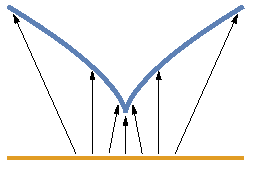
\includegraphics[width=\linewidth]{figures/projective-cuspidal-cubic-birational-map.pdf}
}
下面将在 Example~\ref{ex:projective-cuspidal-cubic-birational-to-line} 中回到这个讨论.
\end{Example}

\begin{Example}{$\mathcal{V}(w^{3}+x^{3}+y^{3})$ 上的有理函数域}\leavevmode\label{ex:irreducible-projective-cubic-not-isomorphic-to-line}
令 $X=\mathcal{V}(w^{3}+x^{3}+y^{3})\subseteq\mathbb{P}^{2}$. 与前一例类似, 可通过计算仿射部分 $X_{0}$ 的函数域来计算 $K(X)$, 得到
\[
  K(X)=K(X_{0})=\operatorname{Frac}\left(\frac{K[x,y]}{\langle1+x^{3}+y^{3}\rangle}\right).
\]
我们在 Example~\ref{ex:fermat-cubic-not-rational} 中证明, 对任意 $d$ 都有 $K(X_{0})\not\cong K(t_{1},\ldots,t_{d})$. 由于同构的簇有同构的有理函数环 (Exercise~\ref{ex:rational-function-rings-invariant-under-isomorphism}), 可知对任意 $d$ 有 $X\not\cong\mathbb{P}^{d}$. 特别地, $X\not\cong\mathbb{P}^{1}$. 这为第~\ref{sec:isomorphisms-of-projective-varieties}~节讨论的一种现象给出了具体例子: 不同于不可约二次曲线, $\mathbb{P}^{2}$ 中的不可约三次曲线不必同构于 $\mathbb{P}^{1}$.
\end{Example}

既然正则函数是正则映射的特例, 可能就会预期有理函数是更一般的有理映射的特例, 事实确实如此. 实际上, 有理映射的定义几乎逐字仿照有理函数的定义.

\begin{Definition}{有理映射}\leavevmode\label{def:rational-map-of-quasiprojective-varieties}
令 $X,Y$ 为拟射影簇. 从 $X$ 到 $Y$ 的一个\emph{有理映射}是数对 $(U,F)$ 的一个等价类, 其中 $U\subseteq X$ 是 $X$ 的稠密开子集, $F:U\to Y$ 是正则映射, 等价关系为
\[
  (U,F)\sim(V,G)\iff F(a)=G(a)\quad\forall a\in U\cap V.
\]
将有理映射记为 $F:X\mathrel{\rightdasharrow} Y$. 有理映射 $F:X\mathrel{\rightdasharrow} Y$ 的\emph{定义域}记为 $U_{F}\subseteq X$, 是 $F$ 的所有代表的定义域的并, 而 $F$ 的\emph{像}为 $F(U_{F})\subseteq Y$.
\end{Definition}

直观地说, 有理映射是拟射影簇之间\textquotedbl{}几乎处处\textquotedbl{}有定义的映射. 在研究有理映射时, 与\textquotedbl{}同构\textquotedbl{}相应的概念是双有理等价.

\begin{Definition}{双有理等价}\leavevmode\label{def:birational-equivalence}
令 $X,Y$ 为拟射影簇. \emph{双有理等价}是有理映射 $F:X\mathrel{\rightdasharrow} Y$, 使存在有理映射 $G:Y\mathrel{\rightdasharrow} X$, 其中 $G\circ F$ 是等价于 $\operatorname{id}_{X}$ 的有理映射, $F\circ G$ 是等价于 $\operatorname{id}_{Y}$ 的有理映射. 若 $X$ 与 $Y$ 之间存在双有理等价, 就称 $X$ 与 $Y$ \emph{双有理}.
\end{Definition}

注意, 复合 $G\circ F$ 定义在 $U_{F}$ 中映入 $U_{G}$ 的点所构成的开集上. 因此 Definition~\ref{def:birational-equivalence} 中要求 $G\circ F$ 是有理映射, 意味着这个集合必在 $X$ 中稠密. 实质上, 双有理的簇\textquotedbl{}几乎处处\textquotedbl{}同构, 给出严格弱于同构的关系. 下一例具体说明一个双有理等价: Example~\ref{ex:projective-cuspidal-cubic-function-field} 的带尖点曲线与射影直线双有理.

\begin{Example}{$\mathcal{V}(wx^{2}-y^{3})$ 与 $\mathbb{P}^{1}$ 双有理}\leavevmode\label{ex:projective-cuspidal-cubic-birational-to-line}
如 Example~\ref{ex:projective-cuspidal-cubic-function-field} 一样, 令 $X=\mathcal{V}(wx^{2}-y^{3})\subseteq\mathbb{P}^{2}$. 则 $X$ 与 $\mathbb{P}^{1}$ 双有理. 为了看出这一点, 考察由下式给出的正则映射 $F:\mathbb{P}^{1}\to X$:
\[
  F([a:b])=[a^{3}:b^{3}:ab^{2}].
\]
虽然 $F$ 没有逆映射, 但有一个有理映射 $G:X\mathrel{\rightdasharrow}\mathbb{P}^{1}$, 由
\[
  G([a:b:c])=[c:b]
\]
给出. 它定义在 $X$ 中 $x$ 和 $y$ 不同时为零的稠密开子集上, 并且作为有理映射与 $G$ 互逆. 从图像上看, 这就是说, 从 $X$ 去掉尖点 $[1:0:0]$ (见 Example~\ref{ex:projective-cuspidal-cubic-function-field}), 从 $\mathbb{P}^{1}$ 去掉它的原像 $[1:0]$ 后, 映射 $F$ 和 $G$ 成为同构.
\end{Example}

正如同构的拟射影簇具有同构的正则函数环, 双有理的拟射影簇具有同构的有理函数环. 例如, 对 Example~\ref{ex:projective-cuspidal-cubic-birational-to-line} 中的 $X$, Example~\ref{ex:projective-cuspidal-cubic-function-field} 的结果表明
\[
  K(X)\cong K(t)\cong K(\mathbb{P}^{1}),
\]
这反映了 Example~\ref{ex:projective-cuspidal-cubic-birational-to-line} 中的双有理等价. 事实上, 与正则函数的情形不同, 上述断言的逆命题也成立. 这里陈述这一结果, 但因为双有理等价在本书余下部分不居核心地位, 把证明留作习题.

\begin{Proposition}{双有理性与有理函数}\leavevmode\label{prop:birational-iff-rational-function-rings-isomorphic}
令 $X,Y$ 为拟射影簇. 则 $X$ 与 $Y$ 双有理, 当且仅当 $K(X)$ 与 $K(Y)$ 是同构的 $K$-代数.
\end{Proposition}
\begin{Proof}
Exercises~\ref{ex:pullback-of-rational-functions-under-dominant-map} 和~\ref{ex:construct-rational-map-from-function-ring-homomorphism}.
\end{Proof}

代数几何中有一个大而活跃的分支, 称为\emph{双有理几何}, 专门按簇之间是否双有理来对簇分类. 由于双有理的簇\textquotedbl{}几乎处处\textquotedbl{}同构, 它们具有某些共同属性: 由 Proposition~\ref{prop:birational-iff-rational-function-rings-isomorphic}, 它们的有理函数环相同, 所以 (如下一节将看到的) 它们的维数相同. 但双有理的簇也可能在关键方面不同. 例如, 一个可能是光滑的 (在下下节将遇到拟射影簇的这一概念), 而另一个可能是奇异的, Example~\ref{ex:projective-cuspidal-cubic-birational-to-line} 中的一对簇正是如此. 为一个给定奇异簇寻找与它双有理的光滑簇, 称为\emph{消解奇点}, 它建立在对奇点作爆破的概念之上, 是代数几何中的基本课题. 本章稍后会进一步略述这个概念.

\BookExerciseHeading
\begin{BookExercises}
  \item\label{ex:dense-open-rational-function-equivalence-relation}
  \begin{enumerate}
    \item 证明 Definition~\ref{def:rational-function-on-quasiprojective-variety} 中的关系是等价关系.
    \item 举例说明, 若不要求开集稠密, Definition~\ref{def:rational-function-on-quasiprojective-variety} 中的关系可能不具有传递性.
  \end{enumerate}
  \item\label{ex:rational-functions-form-algebra} 令 $X$ 为拟射影簇. 给定稠密开子集 $U,V\subseteq X$, 正则函数 $F:U\to K$ 和 $G:V\to K$, 以及标量 $\lambda\in K$, 用自然方式定义和, 积及标量倍数:
  \[
    F+G:U\cap V\to K,\qquad FG:U\cap V\to K,\qquad
    \text{以及 }\lambda F:U\to K.
  \]
  解释为何这些运算在有理函数的等价类上良定义, 并证明它们赋予有理函数的集合以 $K$-代数结构.
  \item\label{ex:rational-function-rings-invariant-under-isomorphism} 令 $X,Y$ 为同构的拟射影簇. 证明它们的有理函数环同构: $K(X)\cong K(Y)$.
  \item\label{ex:prove-rational-function-ring-is-field-criterion} 证明 Proposition~\ref{prop:rational-function-ring-is-field-iff-irreducible}.
  \item\label{ex:rational-function-ring-splits-over-irreducible-components} 令 $X$ 为拟射影簇, 不可约分支为 $X_{1},\ldots,X_{k}$. 证明
  \[
    K(X)=K(X_{1})\oplus\cdots\oplus K(X_{k}).
  \]
  \item\label{ex:affine-space-birational-to-projective-space} 证明 $\mathbb{A}^{n}$ 与 $\mathbb{P}^{n}$ 双有理.
  \item\label{ex:birational-equivalence-iff-dense-open-isomorphism} 令 $X,Y$ 为拟射影簇. 证明 $X$ 与 $Y$ 双有理, 当且仅当存在稠密开子集 $U\subseteq X$ 和 $V\subseteq Y$, 使 $U,V$ 作为拟射影簇同构.
  \item\label{ex:pullback-of-rational-functions-under-dominant-map} 令 $F:X\mathrel{\rightdasharrow} Y$ 为拟射影簇之间的有理映射.
  \begin{enumerate}
    \item 假设 $F$ 的像在 $Y$ 中稠密. 构造拉回同态 $F^{*}:K(Y)\to K(X)$.
    \item 假设 $F$ 为双有理等价. 证明 $F$ 的像在 $Y$ 中稠密, 且 $F^{*}$ 为同构.
  \end{enumerate}
  \item\label{ex:construct-rational-map-from-function-ring-homomorphism} 令 $\phi:K(Y)\to K(X)$ 为 $K$-代数的同态, 其中 $X,Y$ 为拟射影簇.
  \begin{enumerate}
    \item 构造有理映射 $F:X\mathrel{\rightdasharrow} Y$, 使 $F^{*}=\phi$, 其中 $F^{*}$ 如 Exercise~\ref{ex:pullback-of-rational-functions-under-dominant-map} 所述. (提示: 证明 $Y$ 含有稠密仿射开子簇 $V$, 并考察 $V$ 上坐标函数在 $\phi$ 下的像.)
    \item 证明若 $\phi$ 是同构, 则 $F$ 是双有理等价.
  \end{enumerate}
\end{BookExercises}

\section{拟射影簇的维数}\label{sec:dimension-of-quasiprojective-varieties}

本节把维数的概念从仿射簇的情形推广到拟射影簇的情形, 然后利用维数的局部性质, 把仿射情形的关键结果引入更一般的拟射影情形.

首先回顾, 我们曾把不可约仿射簇的维数定义为其函数域的超越次数 (第~\ref{sec:dimension-of-affine-varieties}~节). 此外, 在上一节, 我们引入有理函数, 把函数域的概念推广到拟射影情形. 从这一观点来看, 以下定义自然地推广了仿射情形中维数的定义.

\begin{Definition}{拟射影簇的维数}\leavevmode\label{def:dimension-of-quasiprojective-variety}
不可约拟射影簇 $X$ 的\emph{维数}是其有理函数域在 $K$ 上的超越次数:
\[
  \dim(X)=\operatorname{trdeg}_{K}(K(X)).
\]
非空可约拟射影簇的\emph{维数}是其不可约分支的维数的最大值.
\end{Definition}

在更一般的拟射影情形, 维数的一个本质性质是它的局部性. 特别地, 拟射影簇的维数可以在任一稠密开子集上确定, 下一个结果验证了这一点.

\begin{Proposition}{维数与稠密开子簇}\leavevmode\label{prop:dimension-determined-on-dense-open-subvarieties}
若 $X$ 为拟射影簇, $U\subseteq X$ 为稠密开子集, 则
\[
  \dim(X)=\dim(U).
\]
\end{Proposition}
\begin{Proof}
先假设 $X$ 不可约. 则对任一非空 (因而稠密的) 开子集 $U\subseteq X$, 有 $K(X)=K(U)$ (Proposition~\ref{prop:rational-functions-determined-on-dense-open-subvariety}), 所以 $\operatorname{trdeg}(K(X))=\operatorname{trdeg}(K(U))$, 从而 $\dim(X)=\dim(U)$.

为证明一般情形, 设 $X=X_{1}\cup\cdots\cup X_{k}$ 为 $X$ 的不可约分解. 若 $U\subseteq X$ 开且稠密, 则
\[
  U=(X_{1}\cap U)\cup\cdots\cup(X_{k}\cap U)
\]
是 $U$ 的不可约分解 (Exercise~\ref{ex:irreducible-components-of-dense-open-subvariety}). 由于每个 $X_{i}$ 不可约, 且 $X_{i}\cap U$ 为 $X_{i}$ 的非空开子集, 以上论证蕴含 $\dim(X_{i})=\dim(X_{i}\cap U)$. 因此 $X$ 的不可约分支的最大维数与 $U$ 的不可约分支的最大维数相同, 从而 $\dim(X)=\dim(U)$.
\end{Proof}

Proposition~\ref{prop:dimension-determined-on-dense-open-subvarieties} 提供了一种有用的方法, 将拟射影簇的维数理论归结到仿射情形: 若要知道某个不可约拟射影簇 $X$ 的维数, 只须选取一个仿射开子集 $U\subseteq X$ 并计算 $U$ 的维数. 下面几个例子利用了这一策略.

\begin{Example}{射影空间的维数}\leavevmode\label{ex:dimension-of-projective-space}
由于 $\mathbb{P}^{n}$ 包含 $\mathbb{A}^{n}_{0}=\mathbb{A}^{n}$ 作为稠密开子集, Proposition~\ref{prop:dimension-determined-on-dense-open-subvarieties} 蕴含
\[
  \dim(\mathbb{P}^{n})=\dim(\mathbb{A}^{n})=n.
\]
也可直接由 Definition~\ref{def:dimension-of-quasiprojective-variety} 以及 Example~\ref{ex:projective-function-field-via-affine-patch} 中 $K(\mathbb{P}^{n})=K(x_{1},\ldots,x_{n})$ 的观察得到这个结论.
\end{Example}

\begin{Example}{射影超曲面的维数}\leavevmode\label{ex:dimension-of-projective-hypersurfaces}
令 $f\in K[x_{0},\ldots,x_{n}]$ 为不可约齐次多项式, 考察不可约射影簇
\[
  X=\mathcal{V}_{\mathbb{P}}(f)\subseteq\mathbb{P}^{n}.
\]
我们想计算 $X$ 的维数. 不妨假设 $f\ne x_{0}$, 从而
\[
  X_{0}=\mathcal{V}_{\mathbb{P}}(f)\cap\mathbb{A}^{n}_{0}\ne\varnothing.
\]
因为 $X_{0}$ 是 $X$ 的稠密开子集, Proposition~\ref{prop:dimension-determined-on-dense-open-subvarieties} 蕴含 $X$ 和 $X_{0}$ 具有相同的维数. 而且, 由于 $X_{0}$ 是仿射簇, 可以利用为研究仿射情形中的维数而建立的工具. 特别地, 由于
\[
  X_{0}=\mathcal{V}_{\mathbb{A}}(f_{0})
  \qquad\text{其中}\qquad
  f_{0}(x_{1},\ldots,x_{n})=f(1,x_{1},\ldots,x_{n}),
\]
维数论基本定理 (Theorem~\ref{thm:fundamental-theorem-of-dimension-theory}) 蕴含 $X_{0}$ 的维数为 $n-1$, 因而也有 $\dim(X)=n-1$.

此外, 任一非常数齐次多项式 (不必不可约) 的消没集是其不同不可约因子的消没集的并. 因此, 可以去掉 $f$ 不可约的假设, 得到射影空间中单个非常数齐次多项式的消没集的每个不可约分支的余维都是一.
\end{Example}

\begin{Example}{Grassmann 簇的维数}\leavevmode\label{ex:dimension-of-grassmannians}
考察第~\ref{sec:grassmannians-and-plucker-maps}~节引入的 Grassmann 簇 $\mathrm{G}(k,n)\subseteq\mathbb{P}^{\binom{n}{k}-1}$. 在 Exercise~\ref{ex:grassmannian-affine-charts-and-irreducibility} 中, 要求读者证明 $\mathrm{G}(k,n)$ 不可约, 且其所有仿射限制都同构于 $\mathbb{A}^{k(n-k)}$. 因此, $\mathrm{G}(k,n)$ 包含一个同构于 $k(n-k)$ 维仿射空间的稠密开子簇, 所以
\[
  \dim(\mathrm{G}(k,n))=k(n-k).
\]
为了更直观地理解这个维数, 回顾 $\mathrm{G}(k,n)$ 的元素可以用各行线性无关的 $k\times n$ 矩阵表示. 此外, 在允许换基的意义下, 总可以选取包含一个等于单位矩阵的 $k\times k$ 子矩阵的矩阵表示. 由于剩余的 $k(n-k)$ 个矩阵项可以独立变化, 可见 $\mathrm{G}(k,n)$ 有 $k(n-k)$ 个独立参数, 与上面算出的维数一致.
\end{Example}

为了进一步说明在局部仿射情形下工作的用处, 现在建立拟射影情形中维数论基本定理的推广. 为了以最一般的形式陈述它, 引入局部超曲面的概念. 这是一种新的闭子簇, 局部可由一个正则函数的消没描述. 在下一个定义中, 对任意正则函数 $F\in K[U]$, 采用记号 $\mathcal{V}(F)=\{a\in U\mid F(a)=0\}$. 这是对迄今使用的记号 $\mathcal{V}(-)$ 的小幅而自然的推广.

\begin{Definition}{局部超曲面}\leavevmode\label{def:local-hypersurface}
令 $X$ 为拟射影簇. 若每个 $p\in X$ 都包含在某个开集 $U\subseteq X$ 中, 使 $Y\cap U=\mathcal{V}(F)$, 其中正则函数 $F\in K[U]$ 不在 $U$ 的任何不可约分支上消没, 则称非空子集 $Y\subseteq X$ 为 $X$ 中的\emph{局部超曲面}.
\end{Definition}

Definition~\ref{def:local-hypersurface} 的要点在于, 它为考察拟射影簇 $X\subseteq\mathbb{P}^{n}$ 的两类子簇提供了统一框架: 一类形如 $Y=X\cap\mathcal{V}(F)$, 其中正则函数 $F\in K[X]$ 不在 $X$ 的任何不可约分支上消没; 另一类形如 $Y=X\cap\mathcal{V}(f)$, 其中齐次多项式 $f\in K[x_{0},\ldots,x_{n}]$ 不在 $X$ 的任何不可约分支上消没.

注意, 局部超曲面是 $X$ 的闭子簇. 为了说明这一点, 注意 $\mathcal{V}(F)\subseteq U$ 是单点 $\{0\}$ 在正则映射 $F:U\to\mathbb{A}^{1}$ 下的原像, 因而由正则映射的连续性 (Theorem~\ref{thm:regular-maps-are-zariski-continuous}), 它在 $U$ 中闭. 然后由 Lemma~\ref{lem:closedness-is-local} 得局部超曲面是闭的.

现在陈述这一情形下的维数论基本定理.

\begin{Theorem}{维数论基本定理}\leavevmode\label{thm:fundamental-dimension-theorem-for-quasiprojective-varieties}
令 $X$ 为各不可约分支维数相同的拟射影簇, $Y\subseteq X$ 为 $X$ 中的局部超曲面. 则 $Y$ 的每个不可约分支的维数均为 $\dim(X)-1$.
\end{Theorem}
\begin{Proof}
令 $Z$ 为 $Y$ 的一个不可约分支, $p\in Z$. 由局部超曲面的定义, 存在包含 $p$ 的开子集 $U\subseteq X$ 和正则函数 $F\in K[U]$, 使 $F$ 不在 $U$ 的任何不可约分支上消没, 且
\[
  Y\cap U=\mathcal{V}(F).
\]
必要时限制到一个包含 $p$ 的更小开子集, 可进一步假设 $U$ 是仿射簇. 由于 $Z\cap U$ 不可约, 它必包含在 $U$ 的某个不可约分支中; 将这个分支记为 $V$. 则 $V$ 为不可约仿射簇, 且 $Z\cap V$ 是 $Y\cap V=\mathcal{V}(F|_{V})$ 的一个不可约分支. 由于 $\mathcal{V}(F|_{V})$ 包含 $p$, 且 $F|_{V}\ne0$, $\mathcal{V}(F|_{V})$ 既非空集也不是整个 $V$. 因此仿射情形中维数论基本定理的强形式蕴含
\[
  \dim(Z\cap V)=\dim(V)-1.
\]
$Z$ 的不可约性给出 $\dim(Z)=\dim(Z\cap V)$, 而 $V$ 的不可约性意味着它在 $X$ 的某个分支中稠密. $X$ 的分支的维数都相同, 所以 $\dim(V)=\dim(X)$. 从而 $\dim(Z)=\dim(X)-1$, 如所断言.
\end{Proof}

反复应用上一结果, 得到以下关于拟射影簇内消没集的维数的上界.

\begin{Corollary}{消没集的维数}\leavevmode\label{cor:dimension-bound-for-quasiprojective-vanishing-set}
令 $X\subseteq\mathbb{P}^{n}$ 为各不可约分支维数相同的拟射影簇, $Y=\mathcal{V}(f_{1},\ldots,f_{k},F_{1},\ldots,F_{\ell})\subseteq X$, 其中 $f_{1},\ldots,f_{k}\in K[x_{0},\ldots,x_{n}]$ 齐次, 且 $F_{1},\ldots,F_{\ell}\in K[X]$. 若 $Y\ne\varnothing$, 则
\[
  \dim(Y)\ge\dim(X)-k-\ell.
\]
\end{Corollary}
\begin{Proof}
Exercise~\ref{ex:dimension-bound-for-quasiprojective-vanishing-set}.
\end{Proof}

此外, 与仿射情形完全相同, 维数论基本定理给出维数的以下另一种刻画. 在许多拓扑学情形中, 它被用作维数的定义.

\begin{Corollary}{包含链与维数}\leavevmode\label{cor:dimension-is-length-of-irreducible-closed-chain}
若 $X$ 为拟射影簇, 则 $\dim(X)$ 等于使 $X$ 存在不可约闭子簇 $X_{0},\ldots,X_{d}\subseteq X$ 且满足
\[
  X_{0}\subsetneq X_{1}\subsetneq\cdots\subsetneq X_{d}\subseteq X
\]
的最大 $d$.
\end{Corollary}
\begin{Proof}
Exercise~\ref{ex:dimension-equals-maximal-length-of-chain}.
\end{Proof}

本节最后专门研究齐次多项式方程组的解. 回顾, 研究 $\mathbb{P}^{n}$ 的最初动机之一是找回多项式方程组可能\textquotedbl{}丢在无穷远处\textquotedbl{}的解. 例如, 虽然两条直线在 $\mathbb{A}^{2}$ 中可能不相交, 但我们已经看到它们在 $\mathbb{P}^{2}$ 中总相交. 实质上, $\mathbb{A}^{2}$ 中两条平行直线在 $\mathbb{P}^{2}$ 中的一个\textquotedbl{}无穷远点\textquotedbl{}相交. 下一个结果大幅推广这一观察: $\mathbb{P}^{n}$ 中 $k$ 个超曲面的交的维数总是至少为 $n-k$; 特别地, 只要 $k\le n$, 这个交就一定非空.

\begin{Proposition}{齐次方程组的维数}\leavevmode\label{prop:dimension-of-homogeneous-systems}
若 $f_{1},\ldots,f_{k}\in K[x_{0},\ldots,x_{n}]$ 为非常数齐次多项式且 $k\le n$, 则 $\mathcal{V}_{\mathbb{P}}(f_{1},\ldots,f_{k})\ne\varnothing$, 且
\[
  \dim(\mathcal{V}_{\mathbb{P}}(f_{1},\ldots,f_{k}))\ge n-k.
\]
\end{Proposition}

可以把 Proposition~\ref{prop:dimension-of-homogeneous-systems} 的陈述与仿射情形的 Corollary~\ref{cor:dimension-lower-bound-by-number-of-equations} 的陈述比较. 两个结果的关键区别是, 射影情形可以去掉仿射情形作为假设所需的非空性.

\begingroup
\renewcommand{\AJProofBegin}{%
  \par\addvspace{\topsep}\noindent
  {\sffamily\bfseries\CJKfamily{pffont}Proof of Proposition~\ref{prop:dimension-of-homogeneous-systems}}\enspace\ignorespaces
}
\begin{Proof}
若 $\mathcal{V}_{\mathbb{P}}(f_{1},\ldots,f_{k})\ne\varnothing$, 则 Corollary~\ref{cor:dimension-bound-for-quasiprojective-vanishing-set} 蕴含
\[
  \dim(\mathcal{V}_{\mathbb{P}}(f_{1},\ldots,f_{k}))\ge\dim(\mathbb{P}^{n})-k=n-k.
\]
因此只须证明 $\mathcal{V}_{\mathbb{P}}(f_{1},\ldots,f_{k})\ne\varnothing$. 为此考察仿射消没集
\[
  \mathcal{V}_{\mathbb{A}}(f_{1},\ldots,f_{k})\subseteq\mathbb{A}^{n+1}.
\]
由于 $f_{1},\ldots,f_{k}$ 是非常数齐次多项式, 它们都在原点消没. 因此 $\mathcal{V}_{\mathbb{A}}(f_{1},\ldots,f_{k})\ne\varnothing$, 并且由 Corollary~\ref{cor:dimension-lower-bound-by-number-of-equations} 得
\[
  \dim(\mathcal{V}_{\mathbb{A}}(f_{1},\ldots,f_{k}))\ge n+1-k>0.
\]
由于正维的簇必包含多于一个点, $f_{1},\ldots,f_{k}$ 必在某个非零点 $(a_{0},\ldots,a_{n})\in\mathbb{A}^{n+1}$ 消没. 这意味着 $\mathcal{V}_{\mathbb{P}}(f_{1},\ldots,f_{k})$ 包含点 $[a_{0}:\cdots:a_{n}]\in\mathbb{P}^{n}$. 因此 $\mathcal{V}_{\mathbb{P}}(f_{1},\ldots,f_{k})\ne\varnothing$, 如所需.
\end{Proof}
\endgroup

\BookExerciseHeading
\begin{BookExercises}
  \item\label{ex:quasiprojective-dimension-monotone-and-strict-for-proper-closed-subvariety} 利用维数的局部性, 将以下结果归结为仿射情形下适当的结果, 从而证明它们.
  \begin{enumerate}
    \item 若 $X,Y\subseteq\mathbb{P}^{n}$ 为拟射影簇且 $X\subseteq Y$, 则
    \[
      \dim(X)\le\dim(Y).
    \]
    \item 若进一步有 $Y$ 不可约, 且 $X\subsetneq Y$ 在 $Y$ 中闭, 则
    \[
      \dim(X)<\dim(Y).
    \]
  \end{enumerate}
  \item\label{ex:vanishing-ideal-of-pure-codimension-one-projective-variety-is-principal} 令 $X\subseteq\mathbb{P}^{n}$ 为射影簇, 其每个不可约分支的维数均为 $n-1$. 证明 $\mathcal{I}(X)$ 为主理想, 由 $\mathcal{I}(X)$ 中任一个次数最小的齐次多项式生成.
  \item\label{ex:dimension-bound-for-quasiprojective-vanishing-set} 证明 Corollary~\ref{cor:dimension-bound-for-quasiprojective-vanishing-set}.
  \item\label{ex:dimension-equals-maximal-length-of-chain} 证明 Corollary~\ref{cor:dimension-is-length-of-irreducible-closed-chain}.
  \item\label{ex:dense-image-has-no-larger-dimension-than-domain} 令 $F:X\to Y$ 为拟射影簇之间的正则映射, 使 $F(X)$ 在 $Y$ 中稠密. 证明 $\dim(Y)\le\dim(X)$. (提示: 证明拉回给出单射 $F^{*}:K(Y)\to K(X)$; 见 Exercise~\ref{ex:pullback-of-rational-functions-under-dominant-map}.)
  \item\label{ex:dimension-of-quasiprojective-product} 令 $X,Y$ 为拟射影簇. 证明
  \[
    \dim(X\times Y)=\dim(X)+\dim(Y).
  \]
  \item\label{ex:polynomial-map-from-higher-projective-space-is-constant} 证明当 $n>m$ 时, 每个多项式映射 $\mathbb{P}^{n}\to\mathbb{P}^{m}$ 都是常值的.
  \item\label{ex:regular-map-from-higher-projective-space-is-constant} 证明当 $n>m$ 时, 每个正则映射 $\mathbb{P}^{n}\to\mathbb{P}^{m}$ 都是常值的.
\end{BookExercises}

\section{局部环与切空间}\label{sec:local-rings-and-tangent-spaces}

现在把切空间和光滑性的概念从仿射情形推广到拟射影情形. 初次尝试定义拟射影簇在一点的切空间时, 可能只是限制到该点的某个仿射邻域, 然后使用对应仿射簇在该点的切空间. 这么做确实给出正确的概念, 但它有一个不足: 不同的仿射限制是否给出同一个 (典范同构的) 切空间, 并不立即清楚. 为了避开这一微妙之处, 我们使用局部环建立研究切空间的另一种方法.

大致说来, 拟射影簇 $X$ 在点 $a\in X$ 处的局部环, 表现得像 $a$ 的一个无穷小邻域的坐标环, 这个邻域包含在所有其他邻域中. 局部环是刻画 $X$ 在 $a$ 附近的几何信息的代数工具. 特别地, 可以用它以内在方式定义 $X$ 在 $a$ 处的切空间, 自然地推广 Theorem~\ref{thm:point-ideal-square-quotient-is-dual-of-tangent-space} 中切空间的内在描述. 如将看到的, 这给出了拟射影簇在一点的切空间的一个定义, 当限制到任一仿射邻域时, 它恢复仿射情形中的概念.

我们从一点处局部环的正式定义开始讨论.

\begin{Definition}{拟射影簇在一点处的局部环}\leavevmode\label{def:local-ring-of-quasiprojective-variety-at-point}
令 $X$ 为拟射影簇, $a\in X$. $X$ 在 $a$ 处的\emph{局部环}记为 $K[X]_{a}$, 是数对 $(U,F)$ 的等价类的集合, 其中 $U\subseteq X$ 是包含 $a$ 的 $X$ 的开子集, $F:U\to K$ 是正则函数. 两个数对 $(U,F)$ 与 $(V,G)$ 等价, 当且仅当存在包含 $a$ 的开集 $W\subseteq U\cap V$, 使对所有 $b\in W$ 有 $F(b)=G(b)$.
\end{Definition}

换句话说, $K[X]_{a}$ 的一个元素可由 $a$ 的某个邻域上的正则函数表示. 两个可能定义在不同邻域上的正则函数给出同一个元素, 当且仅当它们在某个可能更小的邻域上相等. 因此, 可把 $X$ 在 $a$ 处的局部环的一个元素看成定义在 $a$ 的任意小邻域上的正则函数. 为此, 把局部环 $K[X]_{a}$ 的元素称为 $a$ 处的\emph{局部函数}.

Definition~\ref{def:local-ring-of-quasiprojective-variety-at-point} 有几个方面需要进一步说明. 例如, 应当停下来理解为什么数对 $(U,F)$ 之间的关系确实是等价关系, 也应仔细定义 $K[X]_{a}$ 上自然的加法, 乘法和标量乘法, 这些代数运算使它成为 $K$-代数 (见 Exercise~\ref{ex:local-ring-equivalence-classes-and-algebra-operations}).

在进一步研究局部环前, 先考察几个具体例子.

\begin{Example}{由多项式的商给出的局部函数}\leavevmode\label{ex:local-functions-from-homogeneous-quotients}
令 $X\subseteq\mathbb{P}^{n}$ 为拟射影簇, $a\in X$. 给定同次数的两个齐次多项式 $f,g\in K[x_{0},\ldots,x_{n}]$, 它们的商定义正则映射 $f/g:X\setminus\mathcal{V}(g)\to K$. 特别地, 若 $g(a)\ne0$, 则 $f/g$ 给出 $a$ 处的一个局部函数, 它定义在邻域 $U=X\setminus\mathcal{V}(g)$ 上. 事实上, 下面将看到每个局部函数都可以实现为多项式的商.
\end{Example}

\begin{Example}{不同的商给出同一个局部函数}\leavevmode\label{ex:local-function-does-not-see-other-irreducible-component}
考察可约射影簇 $X=\mathcal{V}(xy)=\mathcal{V}(x)\cup\mathcal{V}(y)\subseteq\mathbb{P}^{2}$, 令 $a=[1:0:0]$. 注意 $a$ 在不可约分支 $\mathcal{V}(y)$ 中, 但不在不可约分支 $\mathcal{V}(x)$ 中. 考察有理函数
\[
  \frac{x+y}{x-y}:X\setminus\{[0:0:1]\}\to K.
\]
这个有理函数并非恒定, 因为它在 $[1:0:0]$ 处取值 $1$, 在 $[0:1:0]$ 处取值 $-1$. 不过, 它定义的 $a$ 处的局部函数是常值函数 $1$, 原因只在于限制到邻域 $U=X\setminus\mathcal{V}(x)$ 后, 它的分子和分母相同. 这一例子说明局部函数的局部性质: $a$ 处的局部函数\textquotedbl{}看不见\textquotedbl{}不可约分支 $\mathcal{V}(x)\subseteq X$, 因为这个不可约分支不含 $a$.
\end{Example}

以先前例子中的观察为基础, 下一个结果说明拟射影簇 $X$ 在点 $a$ 处的局部环确实只取决于 $a\in X$ 附近的情况: 换句话说, 将其限制到 $a$ 的更小邻域并不影响它.

\begin{Proposition}{局部环只取决于局部}\leavevmode\label{prop:local-ring-unchanged-on-open-neighborhood}
设 $X$ 为拟射影簇, $a\in X$. 若 $U\subseteq X$ 为包含 $a$ 的开子簇, 则
\[
  K[U]_{a}=K[X]_{a}.
\]
\end{Proposition}
\begin{Proof}
令 $X$ 为拟射影簇, $a\in X$, 令 $U\subseteq X$ 为包含 $a$ 的开子簇. 有典范的局部环限制同态
\[
  K[X]_{a}\to K[U]_{a},
\]
它将局部函数 $(V,F)\in K[X]_{a}$ 送到 $(U\cap V,F|_{U\cap V})\in K[U]_{a}$. 注意, 局部函数为 $0$, 当且仅当代表它的任意正则函数在 $a$ 的某个邻域上消没; 这意味着限制映射是单射. 限制映射也是满射, 因为按定义, $K[U]_{a}$ 的每个元素都可视为 $K[X]_{a}$ 的元素, 因而是它自身的限制. 因此 $K[X]_{a}=K[U]_{a}$.
\end{Proof}

由于拟射影簇是局部仿射的, Proposition~\ref{prop:local-ring-unchanged-on-open-neighborhood} 把局部环的研究归结到仿射情形. 因此, 具体描述仿射簇的局部环将是有用的, 现在给出这一描述.

\begin{Lemma}{仿射簇的局部环}\leavevmode\label{lem:local-rings-of-affine-varieties-as-fractions}
令 $X$ 为仿射簇, $a\in X$. $K[X]_{a}$ 的每个元素都可表示为商 $F/G$, 其中 $F,G\in K[X]$ 为正则函数, 且 $G(a)\ne0$. 两个商 $F/G$ 和 $F'/G'$ 给出同一个局部函数, 当且仅当存在 $H\in K[X]$, 使 $H(a)\ne0$, 且
\[
  H(FG'-F'G)=0\in K[X].
\]
\end{Lemma}
\begin{Proof}
由于开集以及开集上的正则函数环在同构下保持, 只须假设 $X$ 为 $\mathbb{A}^{n}_{0}\subseteq\mathbb{P}^{n}$ 的闭子集. 令 $a\in X$, 假设 $(U,H)$ 代表 $K[X]_{a}$ 的一个元素, 因而 $H\in K[U]$. 由正则函数的定义, 存在同为 $d$ 次的齐次多项式 $f,g\in K[x_{0},\ldots,x_{n}]$, 使 $g(a)\ne0$, 且
\[
  H(b)=\frac{f(b)}{g(b)}\qquad\text{对所有 }b\in U\setminus\mathcal{V}(g).
\]
定义 $F=f(x_{0},x_{1},\ldots,x_{n})/x_{0}^{d}$ 和 $G=g(x_{0},\ldots,x_{n})/x_{0}^{d}$. 由于 $F,G$ 各自是同次数的齐次多项式的商, 且分母在 $X$ 上不消没, 可知 $F,G\in K[X]$. 由构造, 有
\[
  H(b)=\frac{F(b)}{G(b)}\qquad\text{对所有 }b\in U\setminus\mathcal{V}(G).
\]
这表明在 $K[X]_{a}$ 中, $(U,H)$ 与 $(X\setminus\mathcal{V}(G),F/G)$ 等价, 所以每个局部函数都可实现为 $X$ 上两个正则函数的商.

现假设 $F/G$ 和 $F'/G'$ 是 $X$ 上正则函数的商, 在 $K[X]_{a}$ 中给出同一个局部函数. 则 $FG'-F'G$ 必在 $a$ 的某个邻域上消没. 由于不可约分支的开子集是稠密的, 且 $FG'-F'G$ 的消没集在 $X$ 中闭, 这蕴含 $FG'-F'G$ 在 $X$ 的每个包含 $a$ 的不可约分支上消没. 令 $H\in K[X]$ 为任一满足 $H(a)\ne0$ 且在 $X$ 的每个不包含 $a$ 的不可约分支上消没的正则函数. 则 $H(FG'-F'G)=0\in K[X]$.

反过来, 假设存在 $F,F',G,G',H\in K[X]$, 后三者均不在 $a$ 处消没, 且 $H(FG'-F'G)=0\in K[X]$. 因而
\[
  F(b)/G(b)=F'(b)/G'(b)\qquad\text{对所有 }b\in X\setminus\mathcal{V}(HGG').
\]
由于 $X\setminus\mathcal{V}(HGG')$ 是 $a$ 的开邻域, 可知 $F/G$ 和 $F'/G'$ 在 $K[X]_{a}$ 中给出同一个局部函数.
\end{Proof}

\BookPairedNoteLeft{
Lemma~\ref{lem:local-rings-of-affine-varieties-as-fractions} 中的描述是更一般的代数过程\textquotedbl{}局部化\textquotedbl{}的动机; 更多细节见 Exercise~\ref{ex:construction-and-examples-of-ring-localization}.
}{
现在从局部环的角度重新考察仿射簇的切空间. 回顾第~\ref{chap:smoothness}~章, 仿射簇 $X$ 在点 $a\in X$ 处的切空间 $T_{a}X$, 首先用切向量和 $a$ 处的梯度作外在定义, 后来又用 $X$ 上在 $a$ 处消没的正则函数构成的极大理想作内在描述.
}
第二种内在观点在局部环的情形有自然的对应, 下面说明.

\BookPairedNote{
令 $X$ 为拟射影簇, $a\in X$, 令 $J_{a}\subseteq K[X]_{a}$ 为在 $a$ 处消没的局部函数构成的理想. 注意, $J_{a}$ 是 $K[X]_{a}$ 的极大理想. 事实上, 它是 $K[X]_{a}$ 中唯一的极大理想 (Exercise~\ref{ex:unique-maximal-ideal-of-local-ring}).
}{
受这一几何情形的启发, 具有唯一极大理想的环通常称为\textquotedbl{}局部环\textquotedbl{}.
}
专门来看仿射情形, 第~\ref{chap:smoothness}~章已经定义了切空间, 现在可用理想 $J_{a}\subseteq K[X]_{a}$ 对切空间作如下另一种描述.

\begin{Proposition}{再论仿射簇的切空间}\leavevmode\label{prop:affine-tangent-space-dual-of-local-maximal-ideal-quotient}
若 $X$ 为仿射簇, $a\in X$, $J_{a}\subseteq K[X]_{a}$ 为在 $a$ 处消没的局部函数的理想, 则有典范的向量空间同构
\[
  T_{a}X=(J_{a}/J_{a}^{2})^{\vee}.
\]
\end{Proposition}
\begin{Proof}
如第~\ref{sec:intrinsic-tangent-spaces}~节, 令 $I_{a}\subseteq K[X]$ 表示在 $a$ 处消没的正则 (即多项式) 函数的极大理想. 由 Theorem~\ref{thm:point-ideal-square-quotient-is-dual-of-tangent-space}, 有典范的向量空间同构
\[
  T_{a}X=(I_{a}/I_{a}^{2})^{\vee}.
\]
因此, 我们必须证明存在典范的向量空间同构
\[
  I_{a}/I_{a}^{2}=J_{a}/J_{a}^{2}.
\]
考察限制同态 $K[X]\to K[X]_{a}$. 稍加思考可知此映射把 $I_{a}$ 送入 $J_{a}$, 把 $I_{a}^{2}$ 送入 $J_{a}^{2}$. 因而得到典范的线性映射
\begin{equation}\label{eq:restriction-map-of-cotangent-quotients}
  I_{a}/I_{a}^{2}\to J_{a}/J_{a}^{2},
\end{equation}
只须再证明这个线性映射是双射.

为证明 \eqref{eq:restriction-map-of-cotangent-quotients} 的满射性, 首先注意, 由 Lemma~\ref{lem:local-rings-of-affine-varieties-as-fractions}, $K[X]_{a}$ 的每个元素都可写成 $F/G$, 其中 $F,G\in K[X]$ 且 $G(a)\ne0$. 假设 $F/G$ 给出 $J_{a}$ 的一个元素, 或等价地, $F\in I_{a}$. 必要时同时缩放 $F$ 和 $G$, 可假设 $G(a)=1$. 因而 $F$ 与 $1/G-1$ 都给出 $J_{a}$ 的元素, 所以
\[
  F/G-F=F(1/G-1)\in J_{a}^{2}.
\]
这意味着 $F/G$ 与 $F$ 定义的局部函数在商 $J_{a}/J_{a}^{2}$ 中等价, 所以 $[F/G]\in J_{a}/J_{a}^{2}$ 是 $[F]\in I_{a}/I_{a}^{2}$ 的像, 从而证得 \eqref{eq:restriction-map-of-cotangent-quotients} 的满射性.

为证明单射性, 假设 $F\in I_{a}$ 限制为属于 $J_{a}^{2}$ 的一个局部函数. $J_{a}^{2}$ 的元素是 $J_{a}$ 中两个元素的乘积的有限和. 因此由 Lemma~\ref{lem:local-rings-of-affine-varieties-as-fractions}, 存在 $m\ge1$ 和 $i=1,\ldots,m$ 时的 $G_{i},G'_{i},H_{i},H'_{i}\in K[X]$, 使对所有 $i=1,\ldots,m$ 有 $G_{i}(a)=0=G'_{i}(a)$ 且 $H_{i}(a)\ne0\ne H'_{i}(a)$, 并存在 $a$ 的邻域 $U$, 使
\[
  F(b)=\sum_{i=1}^{m}\frac{G_{i}(b)G'_{i}(b)}{H_{i}(b)H'_{i}(b)}
  \qquad\text{对所有 }b\in U.
\]
选取 $H\in K[X]$, 使 $H(a)\ne0$ 且 $H$ 在 $X\setminus U$ 上消没. 则
\[
  H(b)F(b)=H(b)\sum_{i=1}^{m}\frac{G_{i}(b)G'_{i}(b)}{H_{i}(b)H'_{i}(b)}
  \qquad\text{对所有 }b\in X.
\]
消去分母后可见 $(H_{1}\cdots H_{m})(H'_{1}\cdots H'_{m})HF\in I_{a}^{2}$. 由于 $F$ 是此乘积中唯一属于 $I_{a}$ 的因子, 可推出 $F\in I_{a}^{2}$ (Exercise~\ref{ex:divide-out-factor-not-in-maximal-ideal-from-square}). 这证明了 \eqref{eq:restriction-map-of-cotangent-quotients} 的单射性, 从而完成证明.
\end{Proof}

前一结果启发了拟射影簇一般情形下切空间的如下内在定义.

\begin{Definition}{拟射影簇的切空间}\leavevmode\label{def:tangent-space-of-quasiprojective-variety}
设 $X$ 为拟射影簇, $a\in X$, 令 $J_{a}$ 表示 $K[X]_{a}$ 中在 $a$ 处消没的局部函数构成的理想. $X$ 在 $a$ 处的\emph{切空间}记为 $T_{a}X$, 是向量空间
\[
  T_{a}X=(J_{a}/J_{a}^{2})^{\vee}.
\]
\end{Definition}

由 Definition~\ref{def:tangent-space-of-quasiprojective-variety} 的局部性, 若 $X$ 为拟射影簇, $a\in X$, $U$ 为 $a$ 的一个邻域, 则 $T_{a}X=T_{a}U$. 特别地, 总可以先限制到一个仿射开邻域, 然后按第~\ref{chap:smoothness}~章中的方法计算拟射影簇的切空间.

由切空间在仿射情形的内在性质还可知, 切空间在拟射影情形也是内在的. 更具体地说, 若 $F:X\to Y$ 是拟射影簇的同构, 且 $F(a)=b$, 则 $F$ 限制为 $a$ 的任一仿射邻域与其在 $Y$ 中的像之间的同构, 而这个像是 $b$ 的仿射邻域. 由仿射情形中切空间的内在性质, 可知 $T_{a}X=T_{b}Y$.

有了拟射影情形中的切空间概念, 自然可以比较切空间的向量空间维数与簇的维数. 通过归结到仿射情形, 首先可观察到, 只要 $X$ 不可约, 就有
\[
  \dim(T_{a}X)\ge\dim(X)
\]
(Exercise~\ref{ex:quasiprojective-tangent-dimension-at-least-variety-dimension}). 与仿射情形一样, 等号成立的点尤其重要.

\begin{Definition}{拟射影簇的光滑性}\leavevmode\label{def:smoothness-of-quasiprojective-variety}
令 $X$ 为不可约拟射影簇, $a\in X$. 若 $\dim(T_{a}X)=\dim(X)$, 就称 $X$ 在 $a$ 处\emph{光滑}; 否则称 $X$ 在 $a$ 处\emph{奇异}. 若 $X$ 在每个点 $a\in X$ 处均光滑, 则称 $X$ \emph{光滑}; 否则称 $X$ \emph{奇异}.
\end{Definition}

由于我们在一般拟射影情形下对切空间和光滑性的建立是局部的, 对这些概念的直观理解可以完全来自仿射情形. 特别地, 拟射影簇在一点处光滑还是奇异, 可以通过限制到该点的一个仿射邻域判定. 因而仿射情形中建立的结果, 例如光滑性的 Jacobian 判据和奇异点集为闭集的事实, 都自然地推广到拟射影情形. 请读者在习题中探究这些结果的射影对应.

注意, 射影情形下的 Jacobian 判据通常比预期多涉及一个偏导数. 本节最后讨论关于 $\mathbb{P}^{n}$ 中超曲面的一个 Jacobian 判据的特例, 由此可见齐次性如何帮助我们处理这个额外的偏导数.

\begin{Example}{射影超曲面的奇点}\leavevmode\label{ex:singularities-of-projective-hypersurfaces}
令 $f\in K[x_{0},\ldots,x_{n}]$ 为不可约齐次多项式, 考察射影超曲面 $X=\mathcal{V}(f)\subseteq\mathbb{P}^{n}$. 我们证明 $X$ 在点 $a\in X$ 处奇异, 当且仅当 $f$ 的所有偏导数都在 $a$ 处消没:
\[
  \frac{\partial f}{\partial x_{0}}(a)=\cdots=\frac{\partial f}{\partial x_{n}}(a)=0.
\]
不妨设 $a\notin\mathcal{V}(x_{0})$, 因而 $a=[1:a_{1}:\cdots:a_{n}]$. 限制到仿射邻域 $X_{0}=X\cap\mathbb{A}^{n}_{0}$, 作自然等同
\[
  X_{0}=\mathcal{V}(f_{0})\subseteq\mathbb{A}^{n}
  \qquad\text{其中}\qquad
  f_{0}(x_{1},\ldots,x_{n})=f(1,x_{1},\ldots,x_{n}).
\]
置 $a=(a_{1},\ldots,a_{n})\in\mathbb{A}^{n}$. 由于 $f$ 不可约, 从而 $f_{0}$ 不可约, 有 $\mathcal{I}(X_{0})=\langle f_{0}\rangle$. 根据仿射情形的 Jacobian 判据 (见 Example~\ref{ex:jacobian-criterion-for-hypersurfaces}), $X_{0}$ 在 $a$ 处奇异, 从而 $X$ 在 $a$ 处奇异, 当且仅当
\[
  \frac{\partial f_{0}}{\partial x_{1}}(a)=\cdots=\frac{\partial f_{0}}{\partial x_{n}}(a)=0.
\]
对偏导数稍作思考可知
\[
  \frac{\partial f}{\partial x_{i}}(1,a_{1},\ldots,a_{n})
  =\frac{\partial f_{0}}{\partial x_{i}}(a_{1},\ldots,a_{n})
  \qquad\text{对所有 }i=1,\ldots,n,
\]
因此 $X$ 在 $a\in X$ 处奇异, 当且仅当
\[
  \frac{\partial f}{\partial x_{1}}(a)=\cdots=\frac{\partial f}{\partial x_{n}}(a)=0.
\]
那么关于 $x_{0}$ 的偏导数呢? 由于 $f$ 是非常数齐次多项式, 齐次多项式的 Euler 恒等式 (Exercise~\ref{ex:euler-identity-for-homogeneous-polynomials}) 给出
\[
  \deg(f)f=x_{0}\frac{\partial f}{\partial x_{0}}+\cdots+x_{n}\frac{\partial f}{\partial x_{n}},
\]
又因为 $f(a)=0$ 且 $a\notin\mathcal{V}(x_{0})$, 可知所有偏导数在 $a$ 处消没, 当且仅当除 $\partial f/\partial x_{0}$ 外的偏导数都在 $a$ 处消没. 因此, $X$ 在 $a\in X$ 处奇异, 当且仅当 $f$ 的所有偏导数都在 $a\in X$ 处消没.
\end{Example}

\BookExerciseHeading
\begin{BookExercises}
  \item\label{ex:local-ring-equivalence-classes-and-algebra-operations}
  \begin{enumerate}
    \item 证明 Definition~\ref{def:local-ring-of-quasiprojective-variety-at-point} 中数对 $(U,F)$ 之间的关系是等价关系.
    \item 仔细定义局部函数的和, 积及标量倍数.
    \item 验证局部环 $K[X]_{a}$ 是 $K$-代数.
  \end{enumerate}
  \item\label{ex:unique-maximal-ideal-of-local-ring} 令 $X$ 为拟射影簇, $a\in X$. 证明 $K[X]_{a}$ 有唯一极大理想 $J_{a}\subseteq K[X]_{a}$, 由所有在 $a$ 处消没的局部函数构成.
  \item\label{ex:divide-out-factor-not-in-maximal-ideal-from-square} 令 $I$ 为环 $R$ 的极大理想, $a,b\in R$ 满足 $a\in I$, $b\notin I$, 且 $ab\in I^{2}$. 证明 $a\in I^{2}$.
  \item\label{ex:quasiprojective-tangent-dimension-at-least-variety-dimension} 令 $X$ 为不可约拟射影簇, $a\in X$. 证明
  \[
    \dim(T_{a}X)\ge\dim(X).
  \]
  (提示: 归结到第~\ref{chap:smoothness}~章中的适当结果.)
  \item\label{ex:smooth-projective-conics-and-singular-projective-cubics}
  \begin{enumerate}
    \item 令 $f\in K[x,y,z]$ 为不可约的二次齐次多项式. 证明 $\mathcal{V}(f)\subseteq\mathbb{P}^{2}$ 光滑.
    \item 举例说明 (a) 不能推广到三次.
  \end{enumerate}
  \item\label{ex:euler-identity-for-homogeneous-polynomials} 令 $f\in K[x_{0},\ldots,x_{n}]$ 为非常数齐次多项式. 证明
  \[
    \deg(f)f=x_{0}\frac{\partial f}{\partial x_{0}}+\cdots+x_{n}\frac{\partial f}{\partial x_{n}}.
  \]
  \item\label{ex:projective-jacobian-criterion} 设 $X\subseteq\mathbb{P}^{n}$ 为不可约射影簇, 消没理想为 $\mathcal{I}(X)=\langle f_{1},\ldots,f_{m}\rangle$. 证明 $X$ 在 $a\in X$ 处奇异, 当且仅当
  \[
    \operatorname{rk}(\operatorname{Jac}_{f_{1},\ldots,f_{m}}(a))<\operatorname{codim}(X).
  \]
  (注: $\operatorname{Jac}_{f_{1},\ldots,f_{m}}(a)$ 不是良定义的, 因为缩放 $a$ 的坐标会缩放 Jacobian 矩阵的各项; 但 Jacobian 的秩是良定义的, 因为这一缩放不影响秩.)
  \item\label{ex:singular-locus-of-irreducible-quasiprojective-variety-is-closed} 证明不可约拟射影簇的奇异点构成一个闭子簇.
  \item\label{ex:construction-and-examples-of-ring-localization} 令 $R$ 为环, $S\subseteq R$ 为对乘法封闭的子集.
  \begin{enumerate}
    \item 考察 $R\times S$ 上的如下关系: 若存在 $t\in S$ 使 $t(rs'-r's)=0$, 则 $(r,s)\sim(r',s')$. 证明 $\sim$ 是等价关系. 等价类的集合称为 $R$ 在 $S$ 处的\emph{局部化}, 记为 $R_{S}$.
    \item 证明 $R_{S}$ 是环, 其运算定义为
    \[
      \begin{aligned}
      (r,s)+(r',s')&=(rs'+r's,ss'),\\
      (r,s)(r',s')&=(rr',ss').
      \end{aligned}
    \]
    此外, 若 $R$ 为 $K$-代数, 证明 $R_{S}$ 为 $K$-代数, 其标量乘法为
    \[
      a(r,s)=(ar,s).
    \]
    \item 若 $R$ 为整环且 $S=R\setminus\{0\}$, 证明
    \[
      R_{S}=\operatorname{Frac}(R).
    \]
    \item 若 $R$ 为环, 且对某个非幂零元 $a\in R$, 有 $S=\{1,a,a^{2},\ldots\}$, 证明
    \[
      R_{S}=R[x]/\langle ax-1\rangle.
    \]
    \item 对某个仿射簇 $X$, 令 $R=K[X]$, 令 $I_{a}\subseteq R$ 为在 $a\in X$ 处消没的函数构成的极大理想. 若 $S=R\setminus I_{a}$, 证明
    \[
      R_{S}=K[X]_{a}.
    \]
  \end{enumerate}
\end{BookExercises}

\section{爆破}\label{sec:blow-ups}

本节通过例子介绍爆破, 这一构造在代数几何中有许多应用. 在各个例子中, 我们着重说明一种特定应用: 用爆破消解奇点. 先从一种非常具体的爆破开始: $\mathbb{A}^{n}$ 在 $0$ 处的爆破. 为便于理解记号, 始终用 $x_{1},\ldots,x_{n}$ 表示 $\mathbb{A}^{n}$ 的坐标, 用 $y_{1},\ldots,y_{n}$ 表示 $\mathbb{P}^{n-1}$ 的齐次坐标 (注意从 $y_{1}$ 开始, 而不是 $y_{0}$).

\begin{Definition}{仿射空间在原点的爆破}\leavevmode\label{def:blowup-of-affine-space-at-origin}
$\mathbb{A}^{n}$ \emph{在原点的爆破}是拟射影簇
\[
  \operatorname{Bl}_{0}(\mathbb{A}^{n})
   =\mathcal{V}(x_{i}y_{j}-x_{j}y_{i}\mid1\le i<j\le n)
    \subseteq\mathbb{A}^{n}\times\mathbb{P}^{n-1},
\]
并配有\emph{爆破映射} $\pi:\operatorname{Bl}_{0}(\mathbb{A}^{n})\to\mathbb{A}^{n}$, 它是 $\mathbb{A}^{n}\times\mathbb{P}^{n-1}$ 到第一因子的投影的限制.
\end{Definition}

在深入探究定义的细节之前, 先用第一个非平凡的情形 $n=2$ 说明它.

\begin{Example}{$\mathbb{A}^{2}$ 在原点的爆破}\leavevmode\label{ex:blowup-of-affine-plane-at-origin}
\BookPairedFigure{
考察 $\mathbb{A}^{2}$ 在原点的爆破,
\[
  \operatorname{Bl}_{0}(\mathbb{A}^{2})
  =\mathcal{V}(x_{1}y_{2}-x_{2}y_{1})\subseteq\mathbb{A}^{2}\times\mathbb{P}^{1}.
\]
右图给出了它在 $\mathbb{R}$ 上的情形, 以及 (向下的) 爆破映射
\[
  \pi:\operatorname{Bl}_{0}(\mathbb{A}^{2})\to\mathbb{A}^{2}.
\]
为理解爆破的这个图示, 考察一点
\[
  \bigl((a_{1},a_{2}),[b_{1},b_{2}]\bigr)\in\operatorname{Bl}_{0}(\mathbb{A}^{2}).
\]
}{
\phantomsection\label{fig:blowup-of-affine-plane}%
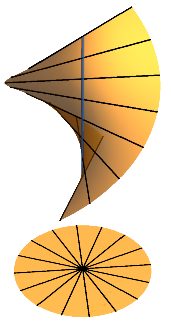
\includegraphics[width=.79\linewidth]{figures/blowup-of-affine-plane.pdf}
}
按定义, 必有 $a_{1}b_{2}=a_{2}b_{1}$. 稍加思考可知, 这等价于 $(a_{1},a_{2})\in\mathbb{A}^{2}$ 位于由 $b=[b_{1}:b_{2}]\in\mathbb{P}^{1}$ 确定的直线上. 换句话说, $\operatorname{Bl}_{0}(\mathbb{A}^{2})$ 中 $\mathbb{P}^{1}$ 坐标固定为 $b$ 的点, 与 $\mathbb{A}^{2}$ 中由点 $b\in\mathbb{P}^{1}$ 参数化的直线上的点有典范对应.

因此在上图中, 我们将 $\mathbb{P}^{1}$ 画作竖直坐标. 此时, $\mathbb{A}^{2}$ 中的每条直线都提升为 $\operatorname{Bl}_{0}(\mathbb{A}^{2})\subseteq\mathbb{A}^{2}\times\mathbb{P}^{1}$ 中同一条直线, 位于该直线所确定的 $\mathbb{P}^{1}$ 坐标的高度. 不过, 这幅图并不完整: 要补全它, 应把 $\operatorname{Bl}_{0}(\mathbb{A}^{2})$ 的顶部绕回来接到底部, 形成一条 Möbius 带, 因为当我们把直线绕原点旋转时, 最终会回到出发处.

注意, 除原点外, $\mathbb{A}^{2}$ 中每一点在 $\operatorname{Bl}_{0}(\mathbb{A}^{2})$ 中都有唯一原像. 这只是说, 这些点中的每一个都确定唯一一条经过原点的直线. 而原点的原像由整个 $\mathbb{P}^{1}$ 构成, 它参数化 $\mathbb{A}^{2}$ 中过原点的所有直线. 换句话说, 在原点对 $\mathbb{A}^{2}$ 作\textquotedbl{}爆破\textquotedbl{}, 可以视为用射影空间 $\mathbb{P}^{1}$ 的一个副本替换 $\mathbb{A}^{2}$ 中的原点.
\end{Example}

\BookPairedNote{
前一例中对 $\operatorname{Bl}_{0}(\mathbb{A}^{2})$ 建立的直观理解, 很自然地推广到 $\operatorname{Bl}_{0}(\mathbb{A}^{n})$. 特别地, 点 $(a,b)\in\mathbb{A}^{n}\times\mathbb{P}^{n-1}$ 在 $\operatorname{Bl}_{0}(\mathbb{A}^{n})$ 上, 当且仅当 $a\in\mathbb{A}^{n}$ 在由 $b\in\mathbb{P}^{n-1}$ 确定的过原点的直线上 (Exercise~\ref{ex:blowup-incidence-condition-is-line-membership}).
}{
\textquotedbl{}爆破\textquotedbl{}这个术语, 最好把它理解为给气球充气或放大图像的比喻, 而不是爆炸的比喻.
}
特别地, 可以把 $\operatorname{Bl}_{0}(\mathbb{A}^{n})$ 看成用整个射影空间 $\mathbb{P}^{n-1}$ 替换 $\mathbb{A}^{n}$ 的原点的结果. 该射影空间参数化所有可能沿着趋近原点的切方向. 除了这一爆破的直观描述, 还应注意 $\operatorname{Bl}_{0}(\mathbb{A}^{n})$ 不可约, 维数为 $n$, 并且光滑 (Exercise~\ref{ex:irreducibility-dimension-and-smoothness-of-affine-space-blowup}).

已经描述 $\mathbb{A}^{n}$ 在原点的爆破, 现在可以定义仿射簇 $X\subseteq\mathbb{A}^{n}$ 在原点的爆破.

\begin{Definition}{仿射簇在原点的爆破}\leavevmode\label{def:blowup-of-affine-variety-at-origin}
令 $X\subseteq\mathbb{A}^{n}$ 为包含原点的 Zariski 闭集. $X$ \emph{在原点的爆破}是拟射影簇
\[
  \operatorname{Bl}_{0}(X)=\overline{\pi^{-1}(X\setminus\{0\})}
    \subseteq\operatorname{Bl}_{0}(\mathbb{A}^{n}).
\]
\end{Definition}

换句话说, 为计算 $X\subseteq\mathbb{A}^{n}$ 在原点的爆破, 先去掉原点, 在 $\operatorname{Bl}_{0}(\mathbb{A}^{n})$ 中考察 $X\setminus\{0\}$ 的原像, 再取 Zariski 闭包. 为获得直观认识, 来看一个具体例子.

\begin{Example}{$\mathbb{A}^{2}$ 中结点曲线的爆破}\leavevmode\label{ex:blowup-of-nodal-affine-curve}
\BookPairedFigure{
考察仿射曲线
\[
  X=\mathcal{V}(x_{1}^{2}+x_{1}^{3}-x_{2}^{2})\subseteq\mathbb{A}^{2},
\]
右侧下图描绘了这条曲线, 上图描绘了它的爆破 $\operatorname{Bl}_{0}(X)$. 为说明 $\operatorname{Bl}_{0}(X)$ 的这一图示, 首先注意 (Exercise~\ref{ex:parametrize-nodal-affine-curve}) 可以把 $X$ 参数化为
\[
  X=\{(a^{2}-1,a^{3}-a)\mid a\in\mathbb{A}^{1}\},
\]
其中 $a=1$ 和 $a=-1$ 都对应原点, $X$ 在这里绕回并与自身相交.
}{
\phantomsection\label{fig:blowup-of-nodal-curve}%
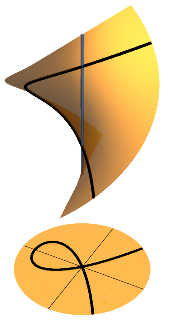
\includegraphics[width=.79\linewidth]{figures/blowup-of-nodal-curve.pdf}
}
由于对所有 $a\ne\pm1$ 有 $[a^{2}-1:a^{3}-a]=[1:a]$, 可推出
\[
  \pi^{-1}(X\setminus\{0\})
  =\{\bigl((a^{2}-1,a^{3}-a),[1:a]\bigr)\mid a\in\mathbb{A}^{1}\setminus\{\pm1\}\}
  \subseteq\mathbb{A}^{2}\times\mathbb{P}^{1}.
\]
为计算 $\pi^{-1}(X\setminus\{0\})$ 的闭包, 只需在上式中补上缺少的两个取值 $a=\pm1$ (Exercise~\ref{ex:closure-and-smoothness-of-nodal-curve-blowup}), 得
\[
  \operatorname{Bl}_{0}(X)=
  \{\bigl((a^{2}-1,a^{3}-a),[1:a]\bigr)\mid a\in\mathbb{A}^{1}\}.
\]
注意原点在 $\operatorname{Bl}_{0}(X)$ 中的原像包含两点 $[1:\pm1]$, 对应 $\mathbb{A}^{2}$ 中斜率为 $\pm1$ 的直线, 它们可视为 $X$ 的两个\textquotedbl{}分支\textquotedbl{}在原点的切线. 因此, 在原点对 $X$ 作爆破, 就按两个分支的斜率把自交点分开了.
\end{Example}

Example~\ref{ex:blowup-of-nodal-affine-curve} 的曲线 $X$ 在原点奇异, 用 Jacobian 判据很容易验证. 但其爆破 $\operatorname{Bl}_{0}(X)$ 同构于 $\mathbb{A}^{1}$ (Exercise~\ref{ex:closure-and-smoothness-of-nodal-curve-blowup}), 所以爆破是光滑的. 换句话说, 爆破\emph{消解}了 $X$ 中的奇点. 更一般地, 拟射影簇 $X$ 的一个\emph{奇点消解}是一个光滑拟射影簇 $Y$ 和一个正则映射 $\pi:Y\to X$, 该映射在 $X$ 的光滑部分的原像上限制为同构. (特别地, 这意味着 $X$ 与 $Y$ 双有理.) 爆破是构造奇点消解的一个重要工具. 下一例进一步说明如何用一次爆破消解曲线的奇点.

\begin{Example}{$\mathbb{A}^{2}$ 中尖点曲线的爆破}\leavevmode\label{ex:blowup-of-cuspidal-affine-curve}
\BookPairedFigure{
考察仿射曲线
\[
  X=\mathcal{V}(x_{1}^{2}-x_{2}^{3})\subseteq\mathbb{A}^{2},
\]
右侧下图描绘了这条曲线, 上图描绘了它的爆破 $\operatorname{Bl}_{0}(X)$. 和前一例一样, 考察 $X$ 的一个参数化:
\[
  X=\{(a^{3},a^{2})\mid a\in\mathbb{A}^{1}\},
\]
其中 $a=0$ 对应原点处的奇点. 对所有 $a\ne0$ 有 $[a^{3}:a^{2}]=[a:1]$.
}{
\phantomsection\label{fig:blowup-of-cuspidal-curve}%
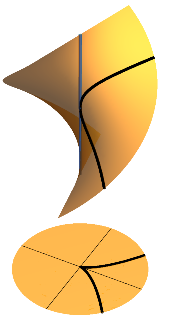
\includegraphics[width=.79\linewidth]{figures/blowup-of-cuspidal-curve.pdf}
}
因此
\[
  \pi^{-1}(X\setminus\{0\})
  =\{\bigl((a^{3},a^{2}),[a:1]\bigr)\mid a\in\mathbb{A}^{1}\setminus\{0\}\}
  \subseteq\mathbb{A}^{2}\times\mathbb{P}^{1}.
\]
和前一例作类似的论证, 在上式中补上取值 $a=0$ 即可算出闭包, 得
\[
  \operatorname{Bl}_{0}(X)=\{\bigl((a^{3},a^{2}),[a:1]\bigr)\mid a\in\mathbb{A}^{1}\}.
\]
和前一例一样, 有 $\operatorname{Bl}_{0}(X)\cong\mathbb{A}^{1}$. 因此再次看到, 爆破 $\operatorname{Bl}_{0}(X)$ 是 $X$ 中尖点奇性的一个消解. 直观地说, 爆破使我们能够用较高维空间中的一条光滑路径来替换 $X$ 在原点处方向的急剧改变.
\end{Example}

到目前为止只看了 $\mathbb{A}^{2}$ 中曲线的爆破. 把维数提高一维, 现在考察 $\mathbb{A}^{3}$ 中曲面的爆破.

\begin{Example}{仿射锥的爆破}\leavevmode\label{ex:blowup-of-affine-cone}
\BookPairedFigure{
考察仿射曲面
\[
  X=\mathcal{V}(x_{1}^{2}+x_{2}^{2}-x_{3}^{2})\subseteq\mathbb{A}^{3}.
\]
在 $\mathbb{R}$ 上, 这是以原点为顶点的圆锥, 如右侧下图所示. 爆破 $\operatorname{Bl}_{0}(X)$ 如上图所示. 为直观理解这里发生了什么, 注意 $X$ 是 $\mathbb{A}^{3}$ 中许多直线的并, 它们都在原点相交. 在原点作爆破, 会把相交的所有这些直线分开, 从而可以把 $\operatorname{Bl}_{0}(X)$ 视为 $\mathbb{A}^{3}\times\mathbb{P}^{2}$ 中这些直线的 (爆破的) \emph{不交}并.
}{
\phantomsection\label{fig:blowup-of-affine-cone}%
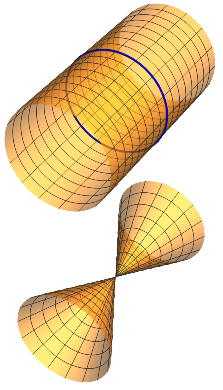
\includegraphics[width=\linewidth]{figures/blowup-of-affine-cone.pdf}
}
在 $\mathbb{R}$ 上工作时, 这些直线的 (爆破的) 不交并可以自然地与上图中的圆柱等同. 不过提醒读者, 在 $\mathbb{C}$ 这样的代数闭域上工作时, $\operatorname{Bl}_{0}(X)$ 的整体几何并没有这么直接.
\end{Example}

本节的例子只是略微触及爆破理论的丰富内容. 有一种更一般的 (内在的) 构造 $\operatorname{Bl}_{Y}(X)$, 沿拟射影簇 $X$ 的一个闭子簇 $Y$ 作爆破. 直观地说, 可通过用参数化该点处法向于 $Y$ 的切方向的射影空间替换 $Y$ 的每一点, 从 $X$ 构造 $\operatorname{Bl}_{Y}(X)$. 爆破理论中最著名的结果是日本数学家 Heisuke Hironaka 在 1964 年证明的奇点消解定理. 它说, 特征零的代数闭域上的每个拟射影簇, 都可以通过一系列爆破消解为光滑簇. 在本节讨论的消解例子中, 消解奇点都只需要一次爆破. 要看必须用两次爆破才能消解的曲线奇点, 请见 Exercise~\ref{ex:two-blowups-resolve-higher-cusp}. 在正特征下, 是否每个簇都能消解仍是一个未解决的问题.

\BookExerciseHeading
\begin{BookExercises}
  \item\label{ex:blowup-incidence-condition-is-line-membership} 证明点 $(a,b)\in\mathbb{A}^{n}\times\mathbb{P}^{n-1}$ 在 $\operatorname{Bl}_{0}(\mathbb{A}^{n})$ 上, 当且仅当 $a$ 在由点 $b\in\mathbb{P}^{n-1}$ 确定的 $\mathbb{A}^{n}$ 中的直线上.
  \item\label{ex:fibres-of-blowup-of-affine-space-at-origin} 考察爆破映射 $\pi:\operatorname{Bl}_{0}(\mathbb{A}^{n})\to\mathbb{A}^{n}$.
  \begin{enumerate}
    \item 证明若点 $(a_{1},\ldots,a_{n})\in\mathbb{A}^{n}$ 的坐标 $a_{i}$ 中至少有一个非零, 则该点的原像为单点.
    \item 证明原点的原像同构于 $\mathbb{P}^{n-1}$.
  \end{enumerate}
  \item\label{ex:irreducibility-dimension-and-smoothness-of-affine-space-blowup}
  \begin{enumerate}
    \item 证明 $\operatorname{Bl}_{0}(\mathbb{A}^{n})$ 有一个同构于 $\mathbb{A}^{n}\setminus\{0\}$ 的稠密开子集.
    \item 证明 $\operatorname{Bl}_{0}(\mathbb{A}^{n})$ 不可约.
    \item 证明 $\operatorname{Bl}_{0}(\mathbb{A}^{n})$ 的维数是 $n$.
    \item 证明 $\operatorname{Bl}_{0}(\mathbb{A}^{n})$ 光滑.
  \end{enumerate}
  \item\label{ex:parametrize-nodal-affine-curve} 令 $X=\mathcal{V}(x_{1}^{2}+x_{1}^{3}-x_{2}^{2})\subseteq\mathbb{A}^{2}$. 证明
  \[
    X=\{(a^{2}-1,a^{3}-a)\mid a\in\mathbb{A}^{1}\}.
  \]
  \item\label{ex:closure-and-smoothness-of-nodal-curve-blowup} 考察子集
  \[
    Y=\{\bigl((a^{2}-1,a^{3}-a),[1:a]\bigr)\mid a\in\mathbb{A}^{1}\setminus\{\pm1\}\}
    \subseteq\mathbb{A}^{2}\times\mathbb{P}^{1}.
  \]
  \begin{enumerate}
    \item 设 $f\in K[x_{1},x_{2},y_{1},y_{2}]$ 在 $Y$ 的每一点处消没. 证明 $f$ 也在两点 $\bigl((0,0),[1:\pm1]\bigr)$ 处消没.
    \item 找出三个多项式 $f_{1},f_{2},f_{3}\in K[x_{1},x_{2},y_{1},y_{2}]$, 使
    \[
      \mathcal{V}(f_{1},f_{2},f_{3})
      =\{\bigl((a^{2}-1,a^{3}-a),[1:a]\bigr)\mid a\in\mathbb{A}^{1}\}
        \subseteq\mathbb{A}^{2}\times\mathbb{P}^{1}.
    \]
    \item 推出
    \[
      \overline{Y}=\{\bigl((a^{2}-1,a^{3}-a),[1:a]\bigr)\mid a\in\mathbb{A}^{1}\}.
    \]
    \item 证明 $\overline{Y}\cong\mathbb{A}^{1}$.
  \end{enumerate}
  \item\label{ex:two-blowups-resolve-higher-cusp} 令 $X=\mathcal{V}(x_{1}^{2}-x_{2}^{5})\subseteq\mathbb{A}^{2}$. 本题说明必须对 $X$ 作两次爆破才能消解其奇点.
  \begin{enumerate}
    \item 证明 $X$ 在原点奇异, 而在其他各点光滑.
    \item 证明 $\operatorname{Bl}_{0}(X)\subseteq\mathbb{A}^{2}\times\mathbb{P}^{1}$ 在点 $\bigl((0,0),[0:1]\bigr)$ 处奇异.
    \item 令 $U\subseteq\mathbb{A}^{2}\times\mathbb{P}^{1}$ 为 $y_{2}\ne0$ 的仿射开子集, 置 $Y=U\cap\operatorname{Bl}_{0}(X)$. 则 $Y$ 为 $\operatorname{Bl}_{0}(X)$ 的仿射开子集, 在 $U\cong\mathbb{A}^{3}$ 的原点处有奇点. 证明 $\operatorname{Bl}_{0}(Y)$ 光滑.
  \end{enumerate}
  \item\label{ex:blowup-extends-direction-map-to-regular-map} 考察由下式给出的有理映射 $F:\mathbb{A}^{n}\mathrel{\rightdasharrow}\mathbb{P}^{n-1}$:
  \[
    F(a_{1},\ldots,a_{n})=[a_{1}:\cdots:a_{n}],
  \]
  它在 $\mathbb{A}^{n}\setminus\{(0,\ldots,0)\}$ 上正则.
  \begin{enumerate}
    \item 证明不存在正则映射 $\widetilde{F}:\mathbb{A}^{n}\to\mathbb{P}^{n-1}$ 在 $\mathbb{A}^{n}\setminus\{(0,\ldots,0)\}$ 上与 $F$ 一致.
    \item 构造正则映射 $G:\operatorname{Bl}_{0}(\mathbb{A}^{n})\to\mathbb{P}^{n-1}$, 使对所有满足 $a\ne(0,\ldots,0)$ 的 $(a,b)\in\operatorname{Bl}_{0}(\mathbb{A}^{n})$ 有 $G(a,b)=F(a)$.
  \end{enumerate}
  本题说明爆破的另一种应用: 对有理映射的定义域作爆破, 往往可以用一个与它双有理的定义域替换原定义域, 使有理映射能够延拓为正则映射.
\end{BookExercises}

\section{纤维维数定理}\label{sec:theorem-on-fiber-dimensions}

现在来到整个代数几何中最核心的结果之一: 纤维维数定理. 为引出我们的讨论, 先简短地退回到线性代数的情形. 秩-零化度定理可以说是线性代数最基本的结果. 它说, 对有限维向量空间之间的任意线性映射 $F:V\to W$, 都有
\[
  \dim(F^{-1}(0))=\dim(V)-\dim(F(V)).
\]
\begin{BookFlowNote}{%
映射的\textquotedbl{}纤维\textquotedbl{}一般指单点的原像:
\[
  F^{-1}(b)=\{a\mid F(a)=b\}.
\]
}
换句话说, 零点上的纤维恰是 $F$ 的零空间, 它的维数是定义域的维数减去 $F$ 的像的维数.

虽然一般的纤维 $F^{-1}(w)$ 并不是 $V$ 的线性子空间, 每个纤维却都与零空间 $F^{-1}(0)$ 密切相关. 特别地, 给定任意 $w\in F(V)$ 和 $v_{0}\in F^{-1}(w)$, 可写
\[
  F^{-1}(w)=F^{-1}(0)+v_{0}=\{v+v_{0}\mid v\in F^{-1}(0)\},
\]
\end{BookFlowNote}
表明每个纤维不过是零空间的一个平移. 因此, 若把子空间的平移的维数定义为该子空间本身的维数, 就得到关于线性映射纤维维数的如下基本结果:
\[
  \dim(F^{-1}(w))=\dim(V)-\dim(F(V))\qquad\text{对所有 }w\in F(V).
\]
下图给出这一结果的一个实例. 一个三维向量空间被映到一个一维向量空间上, 定义域中标出了几个二维纤维.

\BookPairedFigure{
本节的目标是把这种基本关系从线性代数推广到多项式代数, 用拟射影簇取代向量空间, 用正则映射取代线性映射. 要使这一推广成立, 必须作一项重要让步: 在代数几何中, 虽然几乎处处的纤维都有预期的维数, 像中可能有一个闭子集, 其上的纤维比预期大, 但绝不会比预期小. 下面用上一节的一个例子说明这一现象.
}{
\phantomsection\label{fig:linear-map-fibres}%
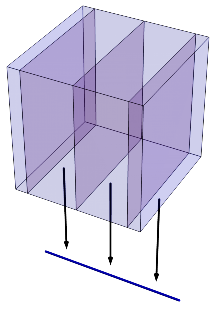
\includegraphics[width=\linewidth]{figures/linear-map-fibres.pdf}
}

\begin{Example}{爆破的纤维}\leavevmode\label{ex:fibres-of-affine-space-blowup}
令 $\pi:\operatorname{Bl}_{0}(\mathbb{A}^{n})\to\mathbb{A}^{n}$ 为爆破映射, 其中 $n>1$. 如上一节所述, $\mathbb{A}^{n}$ 中任意非零点上的纤维为单点, 而原点上的纤维同构于 $\mathbb{P}^{n-1}$. 由于 $\dim(\mathbb{A}^{n})=\dim(\operatorname{Bl}_{0}(\mathbb{A}^{n}))=n$ 且 $\pi$ 为满射, 预期纤维的维数为零. $\mathbb{A}^{n}$ 的每个非零点都符合这一预期, 但特殊点 $0$ 上的纤维的维数为 $n-1$, 大于预期.
\end{Example}

现在陈述纤维维数定理的第一部分, 它说明纤维绝不会比预期的小.

\begin{Theorem}{纤维维数定理, 第一部分}\leavevmode\label{thm:fiber-dimension-lower-bound}
令 $F:X\to Y$ 为拟射影簇之间的正则映射, 其中 $X$ 不可约. 则对任意 $b\in F(X)$, 都有
\[
  \dim(F^{-1}(b))\ge\dim(X)-\dim(\overline{F(X)}).
\]
\end{Theorem}

\BookPairedNoteLeft{
我们取 $F(X)\subseteq Y$ 的闭包, 因为 $F(X)$ 本身不一定是 $Y$ 的子簇. 见 Exercise~\ref{ex:image-of-affine-polynomial-map-not-quasiprojective}.
}{
如将看到的, Theorem~\ref{thm:fiber-dimension-lower-bound} 是维数论基本定理的一个推论. 下一个引理联系了这两个结果, 它实质上断言: 不可约拟射影簇的每一点都可局部用预期数量的方程定义.
}

\begin{Lemma}{$Y$ 中每一点都局部由 $\dim(Y)$ 个方程定义}\leavevmode\label{lem:point-locally-cut-out-by-dimension-many-functions}
若 $Y$ 是 $d$ 维不可约拟射影簇, $b\in Y$, 则存在仿射开子集 $U\subseteq Y$, 其中 $b\in U$, 以及正则函数 $F_{1},\ldots,F_{d}\in K[U]$, 使 $\mathcal{V}(F_{1},\ldots,F_{d})=\{b\}$.
\end{Lemma}
\begin{Proof}
若 $d=0$, 则 $Y=\{b\}$, $U=Y$ 满足所需结论. 故设 $d>0$. 先选取包含 $b$ 的仿射开子集 $V\subseteq Y$. 由于 $Y$ 不可约, $V$ 也不可约, 且 $\dim(V)=d>0$. 在同构意义下, 可以将 $V$ 表示为仿射空间的闭子集 $V\subseteq\mathbb{A}^{n}$. 我们将递归构造多项式 $g_{1},\ldots,g_{d}\in K[y_{1},\ldots,y_{n}]$, 都在 $b$ 处消没, 使 $V\cap\mathcal{V}(g_{1},\ldots,g_{k})$ 的每个不可约分支的维数为 $d-k$.

为开始递归, 选取 $g_{1}\in K[y_{1},\ldots,y_{n}]$, 使它在 $b$ 处消没, 但不在整个 $V$ 上消没 (例如, 若 $b'\in V\setminus\{b\}$ 与 $b$ 的第 $i$ 个坐标不同, 则多项式 $g_{1}=y_{i}-b_{i}$ 就可以). 由于 $V$ 是 $d$ 维不可约簇, 维数论基本定理推出 $V\cap\mathcal{V}(g_{1})$ 的每个不可约分支的维数为 $d-1$.

现假设已经找到 $g_{1},\ldots,g_{k}\in K[y_{1},\ldots,y_{n}]$, 它们都在 $b$ 处消没, 使 $V\cap\mathcal{V}(g_{1},\ldots,g_{k})$ 的每个不可约分支的维数为 $d-k>0$. 由 Exercise~\ref{ex:choose-polynomial-vanishing-at-point-not-on-components}, 可选取 $g_{k+1}\in K[y_{1},\ldots,y_{n}]$, 使它在 $b$ 处消没, 但不在 $V\cap\mathcal{V}(g_{1},\ldots,g_{k})$ 的任何整个不可约分支上消没. 再由维数论基本定理, $V\cap\mathcal{V}(g_{1},\ldots,g_{k},g_{k+1})$ 的每个不可约分支的维数为 $d-k-1$, 如所需.

由构造, $V\cap\mathcal{V}(g_{1},\ldots,g_{d})$ 是零维的, 因而是有限集 $\{b,b_{1},\ldots,b_{\ell}\}$. 令 $U\subseteq V$ 为任一包含于开集 $V\setminus\{b_{1},\ldots,b_{\ell}\}$ 中的 $b$ 的仿射开邻域, 对 $k=1,\ldots,d$ 置 $F_{k}=g_{k}|_{U}$. 则 $F_{1},\ldots,F_{d}$ 是 $U$ 上的正则函数, 且 $\mathcal{V}(F_{1},\ldots,F_{d})=\{b\}$, 证毕.
\end{Proof}

现在证明纤维维数定理的第一部分.

\begingroup
\renewcommand{\AJProofBegin}{%
  \par\addvspace{\topsep}\noindent
  {\sffamily\bfseries\CJKfamily{pffont}Proof of Theorem~\ref{thm:fiber-dimension-lower-bound}}\enspace\ignorespaces
}
\begin{Proof}
由于定理的陈述不涉及 $\overline{F(X)}$ 之外的 $Y$ 的部分, 可假设 $Y=\overline{F(X)}$. 于是 $F:X\to Y$ 为有稠密像的正则映射. $X$ 的不可约性蕴含 $Y$ 不可约 (Exercise~\ref{ex:image-and-closure-of-irreducible-space-are-irreducible}). 令 $b\in F(X)$, 置 $d=\dim(Y)$. 由 Lemma~\ref{lem:point-locally-cut-out-by-dimension-many-functions}, 选取仿射开子集 $U\subseteq Y$ 和正则函数 $F_{1},\ldots,F_{d}\in K[U]$, 使
\[
  \mathcal{V}(F_{1},\ldots,F_{d})=\{b\}.
\]
置 $V=F^{-1}(U)$, 由正则映射的连续性, 这是 $X$ 的一个开子簇. 由于 $X$ 不可约, $V$ 也不可约, 且 $\dim(V)=\dim(X)$. 用 $G:V\to U$ 表示 $F$ 在 $V$ 上的限制, 注意 $F^{-1}(b)=G^{-1}(b)$. 因为 $G(a)=b$ 当且仅当对所有 $i=1,\ldots,d$ 有 $F_{i}(G(a))=0$, 可得
\[
  G^{-1}(b)=\mathcal{V}(G^{*}(F_{1}),\ldots,G^{*}(F_{d})).
\]
由于 $G^{-1}(b)$ 是 $V$ 上 $d$ 个正则函数的消没集, Corollary~\ref{cor:dimension-bound-for-quasiprojective-vanishing-set} 蕴含
\[
  \dim(G^{-1}(b))\ge\dim(V)-d.
\]
由构造, 此不等式正是定理陈述中的断言:
\[
  \dim(F^{-1}(b))\ge\dim(X)-\dim(\overline{F(X)}).
\]
\end{Proof}
\endgroup

现在进入纤维维数定理的第二部分, 也是较难的一部分. 它实质上说明, 在像的某个非空开子集上, 纤维总能达到预期的维数.

\begin{Theorem}{纤维维数定理, 第二部分}\leavevmode\label{thm:fiber-dimension-equality-on-open-subset}
令 $F:X\to Y$ 为拟射影簇之间的正则映射, 其中 $X$ 不可约. 则存在非空开子集 $U\subseteq Y$, 使对每个 $b\in U$, 有 $F^{-1}(b)=\varnothing$, 或者
\[
  \dim(F^{-1}(b))=\dim(X)-\dim(\overline{F(X)}).
\]
\end{Theorem}
\begin{Proof}
如在 Theorem~\ref{thm:fiber-dimension-lower-bound} 的证明中, 假设 $Y=\overline{F(X)}$. 注意 $X$ 的不可约性于是蕴含 $Y$ 不可约. 现在归约到 $X,Y$ 都为仿射簇的情形.

\textbf{(归约到 $Y$ 为仿射簇)} 假设定理在陪域为仿射簇时成立. 令 $F:X\to Y$ 为正则映射, 其中 $X$ 不可约, 且 $\overline{F(X)}=Y$. 对任一非空仿射开集 $V\subseteq Y$, 可将假设应用于 $F$ 在 (开) 原像 $F^{-1}(V)\subseteq X$ 上的限制. 因此, 由假设, 存在非空开集 $U\subseteq V$, 使对所有 $b\in U$,
\[
  F^{-1}(b)=\varnothing\qquad\text{或}\qquad
  \dim(F^{-1}(b))=\dim(F^{-1}(V))-\dim(V).
\]
由于 $X,Y$ 不可约, $F^{-1}(V)\subseteq X$ 和 $V\subseteq Y$ 都是稠密开集, 因而它们的维数分别与 $X,Y$ 相同. 由此可知, 对所有 $b\in U$,
\[
  F^{-1}(b)=\varnothing\qquad\text{或}\qquad
  \dim(F^{-1}(b))=\dim(X)-\dim(Y).
\]
由于 $U$ 是开集 $V\subseteq Y$ 的非空开子集, 它也是 $Y$ 的非空开集. 由此证明, 所选的 $U$ 满足 $F:X\to Y$ 的定理结论. 既然定理的一般形式由陪域为仿射簇的特例推出, 以下假设 $Y$ 为仿射簇.

\textbf{(归约到 $X$ 为仿射簇)} 假设定理在定义域为仿射簇时成立. 令 $F:X\to Y$ 为正则映射, 其中 $X$ 不可约, 且 $\overline{F(X)}=Y$. 由 Theorem~\ref{thm:quasiprojective-varieties-have-finite-affine-open-covers}, 选取有限多个仿射开子集 $V_{1},\ldots,V_{k}\subseteq X$, 使 $X=V_{1}\cup\cdots\cup V_{k}$. 由于 $X$ 不可约, 每个 $V_{i}$ 都在 $X$ 中稠密, 从而 $F(V_{i})$ 在 $Y$ 中稠密 (Exercise~\ref{ex:continuous-map-with-dense-image-maps-dense-subsets-to-dense-subsets}). 令 $F_{i}:V_{i}\to Y$ 为 $F$ 在 $V_{i}$ 上的限制. 由于 $V_{i}$ 仿射且不可约, 又有 $\overline{F_{i}(V_{i})}=Y$, 我们的假设蕴含存在非空开子集 $U_{i}\subseteq Y$, 使对每个 $b\in U_{i}$,
\[
  \begin{aligned}
  F_{i}^{-1}(b)&=\varnothing\\
  \text{或}\qquad\dim(F_{i}^{-1}(b))&=\dim(V_{i})-\dim(Y)=\dim(X)-\dim(Y).
  \end{aligned}
\]
考察非空开集 $U=U_{1}\cap\cdots\cap U_{k}\subseteq Y$, 令 $b\in U$. 若 $Z$ 为 $F^{-1}(b)$ 的一个不可约分支, 则至少对一个 $i$ 有 $V_{i}\cap Z$ 非空, 因为 $X=V_{1}\cup\cdots\cup V_{k}$. 因此
\[
  \dim(Z)=\dim(V_{i}\cap Z)\le\dim(F_{i}^{-1}(b))=\dim(X)-\dim(Y).
\]
第一个等式来自 $Z$ 不可约这一假设, 它蕴含 $V_{i}\cap Z$ 稠密; 不等式来自 $V_{i}\cap Z\subseteq F_{i}^{-1}(b)$; 第二个等式来自 $b\in U_{i}$ 这一假设. 由于已经找到 $F^{-1}(b)$ 的每个不可约分支维数的一致上界, 可知 $\dim(F^{-1}(b))\le\dim(X)-\dim(Y)$. 另一个不等式由 Theorem~\ref{thm:fiber-dimension-lower-bound} 得到. 因此, 已构造非空开集 $U\subseteq Y$, 使对每个 $b\in U$,
\[
  F^{-1}(b)=\varnothing\qquad\text{或}\qquad
  \dim(F^{-1}(b))=\dim(X)-\dim(Y).
\]
既然定理的一般形式由定义域为仿射簇的情形推出, 以下假设 $X$ 为仿射簇.

\textbf{($X$ 和 $Y$ 为仿射簇的证明)} 令 $F:X\to Y$ 为不可约仿射簇之间的正则映射, 使 $\overline{F(X)}=Y$. 由于 $F(X)$ 在 $Y$ 中稠密, 拉回同态 $F^{*}:K[Y]\to K[X]$ 为单射 (Exercise~\ref{ex:density-dominance-and-injective-pullback}). 通过这一单射, 将 $K[Y]$ 视为 $K[X]$ 的子代数. 取分式域后, 也将 $K(Y)$ 视为 $K(X)$ 的子域. 关于超越次数, 有
\begin{equation}\label{eq:transcendence-degree-difference-for-fibres}
  \operatorname{trdeg}_{K(Y)}K(X)
  =\operatorname{trdeg}_{K}K(X)-\operatorname{trdeg}_{K}K(Y),
\end{equation}
因为 $K(Y)$ 在 $K$ 上的每个超越基都能扩充为 $K(X)$ 在 $K$ 上的超越基, 而扩充进去的元素给出 $K(X)$ 在 $K(Y)$ 上的一个超越基 (Exercise~\ref{ex:transcendence-degrees-add-in-tower}).

把 $X$ 写成仿射空间的闭子集 $X\subseteq\mathbb{A}^{m}$, 定义 $A\subseteq K(X)$ 为坐标函数 $[x_{1}],\ldots,[x_{m}]$ 生成的 $K(Y)$-代数:
\[
  A=K(Y)\bigl[[x_{1}],\ldots,[x_{m}]\bigr]\subseteq K(X).
\]
由于 $A$ 在 $K(Y)$ 上由 $[x_{1}],\ldots,[x_{m}]$ 有限生成, Noether 正规化定理保证存在有限的 Noether 基 $\{H_{1},\ldots,H_{e}\}\subseteq A$. 更具体地说, $H_{1},\ldots,H_{e}$ 是 $A$ 中在 $K(Y)$ 上代数独立的元素, 使 $A$ 在 $K(Y)[H_{1},\ldots,H_{e}]$ 上整. 特别地, 对每个 $i=1,\ldots,m$, 都存在首一多项式
\[
  g_{i}(z)\in\bigl(K(Y)[H_{1},\ldots,H_{e}]\bigr)[z],
\]
使 $g_{i}([x_{i}])=0\in A$. 由于 $K(X)=K([x_{1}],\ldots,[x_{m}])$, 且每个 $[x_{i}]$ 在 $K(Y)[H_{1},\ldots,H_{e}]$ 上代数, 可知 Noether 基 $\{H_{1},\ldots,H_{e}\}$ 给出 $K(X)$ 在 $K(Y)$ 上的一个超越基. 于是 \eqref{eq:transcendence-degree-difference-for-fibres} 蕴含
\[
  e=\dim(X)-\dim(Y).
\]
由 $A$ 的定义, 对每个 $i=1,\ldots,e$, 可对某些 $F_{i}\in K[X]$, $G_{i}\in K[Y]\setminus\{0\}$ 写 $H_{i}=F_{i}/G_{i}$. 此外, 把 $g_{i}(z)$ 看作 $H_{1},\ldots,H_{e},z$ 的多项式时, 它的每个系数都是 $K(Y)$ 的元素, 因而可以表示为 $Y$ 上正则函数的商. 令 $G\in K[Y]\setminus\{0\}$ 为 $G_{1},\ldots,G_{e}$ 和 $g_{1}(z),\ldots,g_{e}(z)$ 的系数中作为分母出现的所有 $Y$ 上正则函数的乘积, 定义非空开集
\[
  U=Y\setminus\mathcal{V}(G).
\]
现在论证 $U$ 满足定理的结论.

令 $b\in U$, 假设 $F^{-1}(b)\ne\varnothing$. $U$ 的构造意味着对所有 $i=1,\ldots,e$ 有 $G_{i}(b)\ne0$. 函数 $H_{i}=F_{i}/G_{i}$ 在纤维 $F^{-1}(b)$ 上的限制给出正则函数 $H_{i}^{b}\in K[F^{-1}(b)]$, 定义为
\[
  H_{i}^{b}(a)=\frac{F_{i}(a)}{G_{i}(a)}
  \qquad\text{对每个 }a\in F^{-1}(b).
\]
类似地, 由于 $g_{i}(z)$ 的所有系数在 $U$ 上都是良定义的函数, 可以把多项式 $g_{i}(z)$ 的所有系数限制到纤维 $F^{-1}(b)$, 得到多项式
\[
  g_{i}^{b}(z)\in K[H_{1}^{b},\ldots,H_{e}^{b}][z].
\]
重要的是, 由于 $g_{i}(z)$ 首一, $g_{i}^{b}(z)$ 也首一. 因为 $F^{-1}(b)$ 在闭集 $X\subseteq\mathbb{A}^{m}$ 中闭, 坐标函数 $[x_{1}],\ldots,[x_{m}]$ 生成 $K[F^{-1}(b)]$. 将关系 $g_{i}([x_{i}])=0$ 限制到纤维 $F^{-1}(b)$, 得到关系 $g_{i}^{b}([x_{i}])=0\in K[F^{-1}(b)]$, 说明每个坐标函数都在 $K[H_{1}^{b},\ldots,H_{e}^{b}]$ 上整. 因此, Theorem~\ref{thm:finite-generation-integrality} 蕴含 $K[F^{-1}(b)]$ 在 $K[H_{1}^{b},\ldots,H_{e}^{b}]$ 上整. 由 Corollary~\ref{cor:bounds-on-transcendence-degree} 的第~\ref{part:transcendence-degree-upper-bound}~项, 可知
\[
  \dim(F^{-1}(b))\le e=\dim(X)-\dim(Y).
\]
结合 Theorem~\ref{thm:fiber-dimension-lower-bound}, 可得
\[
  \dim(F^{-1}(b))=\dim(X)-\dim(Y),
\]
定理得证.
\end{Proof}

下一例简要说明上一证明所用的几个关键想法.

\begin{Example}{Theorem~\ref{thm:fiber-dimension-equality-on-open-subset} 的证明示例}\leavevmode\label{ex:fiber-dimension-equality-by-clearing-denominators}
考察 $X=\mathcal{V}(xy_{1}-y_{2})\subseteq\mathbb{A}^{3}$ 和 $Y=\mathbb{A}^{2}$, 令 $F:X\to\mathbb{A}^{2}$ 为由 $F(a,b_{1},b_{2})=(b_{1},b_{2})$ 定义的正则映射. 稍加思考 (Exercise~\ref{ex:fibres-of-projection-from-affine-graph}) 可知, $\overline{F(X)}=Y$, $\dim(X)=\dim(Y)=2$, $F(X)$ 的任意非零点上的纤维是一个点, 而 $(0,0)$ 上的纤维同构于 $\mathbb{A}^{1}$. 本例的目标是针对这一具体的仿射簇之间的映射, 逐步说明 Theorem~\ref{thm:fiber-dimension-equality-on-open-subset} 的证明细节, 最终构造非空开集 $U\subseteq Y$, 使 $F$ 在其上的非空纤维都有预期的维数零.

注意 $K(Y)=K(y_{1},y_{2})$, 而 Theorem~\ref{thm:fiber-dimension-equality-on-open-subset} 的证明中出现的代数 $A$ 是
\[
  A=K(y_{1},y_{2})\bigl[[x]\bigr]\subseteq K(X).
\]
空集是 $A$ 在 $K(y_{1},y_{2})$ 上的一个 Noether 基, 因为唯一的生成元 $[x]$ 是首一多项式
\[
  g(z)=z-\frac{y_{2}}{y_{1}}\in K(y_{1},y_{2})[z]
\]
的一个根; 这是因为 $xy_{1}-y_{2}\in\mathcal{I}(X)$. 仿照 Theorem~\ref{thm:fiber-dimension-equality-on-open-subset} 的证明, 令 $G\in K[Y]=K[y_{1},y_{2}]$ 为 Noether 基和首一多项式中出现的所有分母的乘积. 此处 $G=y_{1}$, 所以 $U=\mathbb{A}^{2}\setminus\mathcal{V}(y_{1})$. 因此对任意 $(b_{1},b_{2})\in U$, 都有 $b_{1}\ne0$; 对任意 $(a,b_{1},b_{2})\in F^{-1}(b_{1},b_{2})$, 都得到良定义的首一关系
\[
  0=g(a)=a-\frac{b_{2}}{b_{1}}.
\]
在本例中, 这个关系从 $(b_{1},b_{2})$ 唯一确定 $a$, 表明 $U$ 上的纤维的维数为零, 如所预期.
\end{Example}

本节的最后一个结果是纤维维数定理的一个应用, 它提供了一种验证簇不可约的有用方法.

\begin{Theorem}{等维不可约纤维 $\implies$ 不可约}\leavevmode\label{thm:projective-domain-irreducible-from-equidimensional-irreducible-fibres}
令 $F:X\to Y$ 为满的正则映射, 其中 $X$ 射影, $Y$ 不可约. 若对每个 $b\in Y$, $F^{-1}(b)$ 不可约且维数相同, 则 $X$ 不可约.
\end{Theorem}
\begin{Proof}
令 $X_{1},\ldots,X_{k}$ 为 $X$ 的不可约分支; 我们要证明对某个 $i$ 有 $X=X_{i}$. 令 $F_{i}:X_{i}\to Y$ 为 $F$ 在 $X_{i}$ 上的限制. 由于 $X$ 射影, Theorem~\ref{thm:regular-images-of-projective-varieties-are-closed} 蕴含 $F(X_{i})$ 对每个 $i$ 都在 $Y$ 中闭. 又因为 $F$ 是满射, 可推出
\[
  Y=F(X)=\bigcup_{i=1}^{k}F(X_{i}).
\]
注意 $Y$ 的不可约性意味着至少对一个 $i$ 有 $Y=F(X_{i})$. 对每个满足 $F(X_{i})=Y$ 的 $i$, Theorem~\ref{thm:fiber-dimension-equality-on-open-subset} 蕴含存在非空开集 $U_{i}\subseteq Y$, 使
\[
  \dim(F_{i}^{-1}(b))=\dim(X_{i})-\dim(Y)\qquad\text{对所有 }b\in U_{i}.
\]
对每个满足 $F(X_{i})\ne Y$ 的 $i$, 置 $U_{i}=Y\setminus F(X_{i})$. 令 $U=U_{1}\cap\cdots\cap U_{k}$, 它是 $Y$ 的非空开子集.

选取某个 $b_{0}\in U$. 则 $F^{-1}(b_{0})$ 的不可约性蕴含它包含于某个 $X_{i}$. 不妨设 $F^{-1}(b_{0})\subseteq X_{1}$, 故 $F^{-1}(b_{0})=F_{1}^{-1}(b_{0})$. 由 $U$ 的定义可知 $F_{1}$ 为满射, 且
\[
  \dim(F^{-1}(b_{0}))=\dim(F_{1}^{-1}(b_{0}))=\dim(X_{1})-\dim(Y).
\]
现任取 $b\in Y$. 由于 $F$ 的所有纤维维数相同,
\begin{equation}\label{eq:common-fibre-dimension-from-surjective-component}
  \dim(F^{-1}(b))=\dim(F^{-1}(b_{0}))=\dim(X_{1})-\dim(Y).
\end{equation}
此外, 由 Theorem~\ref{thm:fiber-dimension-lower-bound}, 有
\begin{equation}\label{eq:fibre-dimension-lower-bound-for-surjective-component}
  \dim(F_{1}^{-1}(b))\ge\dim(X_{1})-\dim(Y).
\end{equation}
结合 \eqref{eq:common-fibre-dimension-from-surjective-component} 和 \eqref{eq:fibre-dimension-lower-bound-for-surjective-component}, 得 $\dim(F^{-1}(b))\le\dim(F_{1}^{-1}(b))$. 不过, 由于 $F_{1}^{-1}(b)\subseteq F^{-1}(b)$, 也得到反向不等式, 因而 $\dim(F_{1}^{-1}(b))=\dim(F^{-1}(b))$. 由假设 $F^{-1}(b)$ 不可约, 且 $F_{1}^{-1}(b)=F^{-1}(b)\cap X_{1}$ 是 $F^{-1}(b)$ 的同维闭子集, 可知 (Exercise~\ref{ex:quasiprojective-dimension-monotone-and-strict-for-proper-closed-subvariety}) $F^{-1}(b)=F_{1}^{-1}(b)$. 由于这对所有 $b\in Y$ 成立, 得 $X=X_{1}$, 如所需.
\end{Proof}

\BookExerciseHeading
\begin{BookExercises}
  \item\label{ex:image-of-affine-polynomial-map-not-quasiprojective} 令 $F:\mathbb{A}^{2}\to\mathbb{A}^{2}$ 由 $F(a_{1},a_{2})=(a_{1},a_{1}a_{2})$ 定义.
  \begin{enumerate}
    \item 计算 $F(\mathbb{A}^{2})\subseteq\mathbb{A}^{2}$.
    \item 证明 $F(\mathbb{A}^{2})$ 不是 $\mathbb{A}^{2}$ 的子簇.
    \item 对任意 $(b_{1},b_{2})\in\mathbb{A}^{2}$, 计算纤维 $F^{-1}(b_{1},b_{2})$.
  \end{enumerate}
  \item\label{ex:choose-polynomial-vanishing-at-point-not-on-components}
  \begin{enumerate}
    \item 令 $a_{0},a_{1},\ldots,a_{k}\subseteq\mathbb{A}^{n}$ 为 $\mathbb{A}^{n}$ 中互不相同的点. 证明存在 $f\in K[x_{1},\ldots,x_{n}]$, 使 $f(a_{i})=0$ 当且仅当 $i=0$.
    \item 令 $a\in\mathbb{A}^{n}$, $X_{1},\ldots,X_{k}\subseteq\mathbb{A}^{n}$ 为非空子集, 没有一个等于 $\{a\}$. 证明存在 $f\in K[x_{1},\ldots,x_{n}]$, 使 $f(a)=0$, 且对所有 $i=1,\ldots,k$ 有 $f\notin\mathcal{I}(X_{i})$.
  \end{enumerate}
  \item\label{ex:image-and-closure-of-irreducible-space-are-irreducible} 令 $F:X\to Y$ 为拓扑空间之间的连续映射, $X$ 不可约. 证明 $F(X)$ 和 $\overline{F(X)}$ 都是 $Y$ 的不可约子空间.
  \item\label{ex:continuous-map-with-dense-image-maps-dense-subsets-to-dense-subsets} 设 $F:X\to Y$ 为拓扑空间之间的连续映射, 使 $F(X)$ 在 $Y$ 中稠密. 证明若 $U$ 在 $X$ 中稠密, 则 $F(U)$ 在 $Y$ 中稠密.
  \item\label{ex:transcendence-degrees-add-in-tower} 令 $K\subseteq L\subseteq M$ 为域, 使 $L$ 在 $K$ 上有限生成, $M$ 在 $L$ 上有限生成. 证明
  \[
    \operatorname{trdeg}_{K}(M)
    =\operatorname{trdeg}_{K}(L)+\operatorname{trdeg}_{L}(M).
  \]
  \item\label{ex:fibres-of-projection-from-affine-graph} 置 $X=\mathcal{V}(xy_{1}-y_{2})\subseteq\mathbb{A}^{3}$ 和 $Y=\mathbb{A}^{2}$, 令 $F:X\to\mathbb{A}^{2}$ 为由 $F(a,b_{1},b_{2})=(b_{1},b_{2})$ 定义的正则映射.
  \begin{enumerate}
    \item 证明 $\overline{F(X)}=Y$.
    \item 证明 $\dim(X)=\dim(Y)=2$.
    \item 证明 $F$ 在 $\mathbb{A}^{2}$ 的任意非零点上的纤维或者为空, 或者为单点.
    \item 证明 $F^{-1}(0,0)$ 同构于 $\mathbb{A}^{1}$.
  \end{enumerate}
  \item\label{ex:fibre-dimension-sets-closed-for-projective-maps} 令 $F:X\to Y$ 为射影簇之间的满的正则映射. 证明集合
  \[
    Y_{k}=\{b\in Y\mid\dim(F^{-1}(b))\ge k\}
  \]
  在 $Y$ 中闭.
\end{BookExercises}

\par\medskip
{\footnotesize
\noindent\textbf{开放获取.} 本章按照
\href{http://creativecommons.org/licenses/by-nc/4.0/}{Creative Commons Attribution-NonCommercial 4.0 International License}
的条款授权. 该许可允许以任何媒介或格式进行非商业性使用, 分享, 改编, 分发和复制, 但须对原作者和来源作适当署名, 提供 Creative Commons 许可的链接, 并说明是否作了修改.

\noindent
\begin{minipage}[t]{.17\linewidth}
  \vspace{0pt}
\includegraphics[width=.9\linewidth]{figures/source-cc-by-nc.png}
\end{minipage}\hfill
\begin{minipage}[t]{.81\linewidth}
  \vspace{0pt}本章的图片或其他第三方材料均纳入本章的 Creative Commons 许可, 除非材料的署名行另有注明. 如果材料未纳入本章的 Creative Commons 许可, 且您拟进行的使用未获法律规定的许可或超出允许使用的范围, 则须直接向著作权持有人取得许可.
\end{minipage}\par}

\section{曲面上的直线}\label{sec:lines-on-surfaces}

在本书最后两节中, 我们研究曲面上的直线, 最终目的是证明一个经典事实: 每个光滑三次曲面恰好包含 $27$ 条直线. 实际上, 证明这个经典结果时最棘手的部分之一, 是证明每个三次曲面至少包含一条直线; 本节将把这一事实作为纤维维数定理的应用来证明. 为此, 先退一步, 明确我们所说的 $\mathbb{P}^{3}$ 中曲面的次数是什么意思.

就接下来的两节而言, $\mathbb{P}^{3}$ 中的曲面指任意二维不可约射影簇 $X\subseteq\mathbb{P}^{3}$. 若 $X\subseteq\mathbb{P}^{3}$ 是一个曲面, 则 $\mathcal{I}(X)$ 是由任意在 $X$ 上消没的不可约多项式生成的主理想 (Exercise~\ref{ex:vanishing-ideal-of-pure-codimension-one-projective-variety-is-principal}). 由于主理想的任意两个生成元只相差一个标量因子, 以下概念是良定义的.

\begin{Definition}{$\mathbb{P}^{3}$ 中曲面的次数}\leavevmode\label{def:degree-of-surface-in-projective-three-space}
令 $X\subseteq\mathbb{P}^{3}$ 为一个曲面. $X$ 在 $\mathbb{P}^{3}$ 中的\emph{次数}是 $\mathcal{I}(X)$ 任一生成元的多项式次数.
\end{Definition}

\BookPairedNote{
更一般地, 可以定义任意射影簇 $X\subseteq\mathbb{P}^{n}$ 的次数. 对 $\mathbb{P}^{n}$ 中的超曲面 $X$, 次数就是 $\mathcal{I}(X)$ 任一生成元的次数. 但对于 $\mathbb{P}^{n}$ 中余维更高的射影簇, 次数的概念要复杂一些, 不那么容易精确定义.
}{
直观上, $\mathbb{P}^{n}$ 中一个簇的次数衡量的是它有多\textquotedbl{}弯曲\textquotedbl{}.
}

由于生成曲面 $X\subseteq\mathbb{P}^{3}$ 的消没理想的两个多项式只相差一个标量因子, 我们现在换一个角度, 不再考虑曲面, 而直接研究在相差非零标量因子的意义下的多项式.

\begin{BookNotation}[$\ensuremath{K[x_{0},x_{1},x_{2},x_{3}]_{d}}$ 和 $\mathbb{P}_{3,d}$]\leavevmode\label{notation:projective-space-of-degree-d-polynomials}
令 $K[x_{0},x_{1},x_{2},x_{3}]_{d}$ 为 $K[x_{0},x_{1},x_{2},x_{3}]$ 中由 $d$ 次齐次多项式构成的线性子空间, 并定义
\[
  \mathbb{P}_{3,d}=\frac{K[x_{0},x_{1},x_{2},x_{3}]_{d}\setminus\{0\}}{\sim},
\]
其中当对某个 $\lambda\in K\setminus\{0\}$ 有 $f=\lambda g$ 时, $f\sim g$.
\end{BookNotation}

我们自然地将 $\mathbb{P}_{3,d}$ 等同于以 $K[x_{0},x_{1},x_{2},x_{3}]_{d}$ 中多项式的系数为坐标的射影空间:
\[
  \mathbb{P}_{3,d}=\mathbb{P}^{\binom{d+3}{3}-1}.
\]
每个 $d$ 次曲面自然对应射影空间 $\mathbb{P}_{3,d}$ 中的一个点: 若 $\mathcal{I}(X)=\langle f\rangle$, 就将 $X$ 与 $[f]\in\mathbb{P}_{3,d}$ 等同. 由前面的讨论可知, 这是良定义的. 然而, 并非 $\mathbb{P}_{3,d}$ 的每一点都对应 $\mathbb{P}^{3}$ 中的一个 $d$ 次曲面, 因为其中一些点, 例如 $[x_{0}^{d}]$, 对应可约多项式, 所以它们不定义 (不可约) 曲面.

虽说从研究 $d$ 次曲面的角度看, $\mathbb{P}_{3,d}$ 含有多余的点, 但加上这些点的好处是可以在一个射影空间中工作, 而不是在射影空间的一个子集中工作. 关于 $\mathbb{P}_{3,d}$ 中各点的统一结论, 一经证明, 应用到曲面所对应的点上, 就给出关于所有 $d$ 次曲面的结论.

作为研究曲面上直线的准备, 提醒读者, $\mathbb{P}^{3}$ 中的直线 $L$ 有几种不同的看法, 我们会交替使用:
\begin{itemize}
  \item 将它视为消没集 $\mathcal{V}(\ell_{0},\ell_{1})\subseteq\mathbb{P}^{3}$, 其中 $\ell_{0},\ell_{1}\in K[x_{0},x_{1},x_{2},x_{3}]_{1}$ 是一对线性无关的齐次线性多项式;
  \item 将它视为 $\mathbb{P}(V)=\dfrac{V\setminus\{0\}}{\sim}$, 其中 $V\subseteq K^{4}$ 是二维线性子空间;
  \item 将它视为单射的线性映射 $\mathbb{P}^{1}\to\mathbb{P}^{3}$ 的像.
\end{itemize}
还要回顾, $\mathbb{P}^{3}$ 中的直线由 Grassmann 簇 $\mathrm{G}(2,4)$ 参数化. 借助 Plücker 映射 (Section~\ref{sec:grassmannians-and-plucker-maps}), 我们把它看作 $\mathbb{P}^{5}$ 中的一个射影超曲面.

现在转向本节的主要问题: 给定 $[f]\in\mathbb{P}_{3,d}$, 曲面 $\mathcal{V}(f)\subseteq\mathbb{P}^{3}$ 是否包含一条直线? 先从 $d=3$ 的一个具体例子开始.

\begin{Example}{Fermat 三次曲面上的一条直线}\leavevmode\label{ex:line-on-fermat-cubic-surface}
\BookPairedFigure{
令 $K=\mathbb{C}$, 考察不可约三次多项式 $f=x_{0}^{3}+x_{1}^{3}+x_{2}^{3}+x_{3}^{3}$, 通常称为\textquotedbl{}Fermat 三次式\textquotedbl{}. 令 $L\subseteq\mathbb{P}^{3}$ 为由下式定义的直线:
\[
  L=\{[a:b:-a:-b]\mid [a:b]\in\mathbb{P}^{1}\}\subseteq\mathbb{P}^{3}.
\]
易验证 $f$ 在 $L$ 的每一点处消没, 因此 $L\subseteq\mathcal{V}(f)$.
}{
\phantomsection\label{fig:fermat-cubic-with-line}%
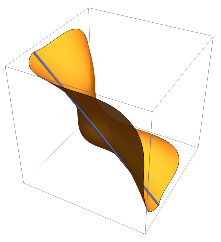
\includegraphics[width=\linewidth]{figures/fermat-cubic-with-line.pdf}
}
图中画出了 $\mathcal{V}(f)$ 和 $L$ 的仿射限制 (的实点).
\end{Example}

上一例给出了一个包含直线的特定三次曲面, 而我们的目标是证明每个三次曲面都包含一条直线. 后一个断言要难证得多. 为这一更一般的结论做准备, 先讨论比较初等的情形: 平面中的直线 ($d=1$) 和二次曲面中的直线 ($d=2$).

在 $d=1$ 时, 多项式 $f\in K[x_{0},x_{1},x_{2},x_{3}]_{1}$ 定义平面 $P=\mathcal{V}(f)\subseteq\mathbb{P}^{3}$. 由于每个平面都包含直线, 实际上, 每个平面都包含无穷多条由 $\mathrm{G}(2,3)\cong\mathbb{P}^{2}$ 参数化的直线, 所以对任意 $[f]\in\mathbb{P}_{3,1}$, 射影簇 $\mathcal{V}(f)\subseteq\mathbb{P}^{3}$ 包含无穷多条直线, 这些直线可由 $\mathbb{P}^{2}$ 参数化.

$d=2$ 的情形稍难一些, 我们在下一个结果中处理它.

\begin{Proposition}{二次曲面由直线覆盖}\leavevmode\label{prop:quadric-surfaces-are-covered-by-lines}
给定 $[f]\in\mathbb{P}_{3,2}$ 和 $a\in\mathcal{V}(f)$, 至少存在一条直线 $L\subseteq\mathbb{P}^{3}$, 使 $a\in L\subseteq\mathcal{V}(f)$. 特别地, $\mathcal{V}(f)$ 包含无穷多条直线.
\end{Proposition}
\begin{Proof}
令 $f\in K[x_{0},x_{1},x_{2},x_{3}]_{2}$ 为齐次二次多项式, 令 $a\in\mathcal{V}(f)\subseteq\mathbb{P}^{3}$. 写 $a=[a_{0}:a_{1}:a_{2}:a_{3}]$, 不妨设 $a_{0}=1$. 限制在仿射开片 $\mathbb{A}_{0}^{3}=\mathbb{A}^{3}$ 上, $\mathbb{P}^{3}$ 中经过 $a$ 的任意直线都由其仿射限制唯一确定, 此仿射限制是形如
\[
  L_{b}=\{(a_{1},a_{2},a_{3})+t(b_{1},b_{2},b_{3})\mid t\in K\}
\]
的仿射直线, 其中 $b=(b_{1},b_{2},b_{3})\ne(0,0,0)$. 由于 $L_{b}$ 不随 $b$ 的缩放而改变, 我们将 $b=[b_{1}:b_{2}:b_{3}]$ 视为 $\mathbb{P}^{2}$ 的元素.

若 $L$ 是经过 $a$ 的一条直线, 则 $f$ 在 $L$ 上消没当且仅当 $f_{0}=f(1,x_{1},x_{2},x_{3})$ 在 $L$ 的仿射限制上消没. 在这样的仿射限制 $L_{b}$ 的每一点上对 $f_{0}$ 求值, 并合并 $t$ 的同次幂, 得到形如
\begin{equation}\label{eq:degree-two-restriction-to-affine-line-through-point}
  f_{0}(a_{1}+tb_{1},a_{2}+tb_{2},a_{3}+tb_{3})
  =g_{1}(b_{1},b_{2},b_{3})t+g_{2}(b_{1},b_{2},b_{3})t^{2},
\end{equation}
的式子, 其中 $g_{i}$ 是 $i$ 次齐次的, 而 $t^{0}$ 项为零, 因为 $f_{0}(a_{1},a_{2},a_{3})=0$. 因此, $f_{0}$ 在 $L_{b}$ 上消没当且仅当 $b\in\mathcal{V}(g_{1},g_{2})$. 由于任意两个齐次多项式在 $\mathbb{P}^{2}$ 中的公共消没集非空 (Proposition~\ref{prop:dimension-of-homogeneous-systems}), 至少存在一个解 $b\in\mathcal{V}(g_{1},g_{2})\in\mathbb{P}^{2}$, 从而至少存在一条直线 $L=\overline{L_{b}}\subseteq\mathbb{P}^{3}$, 使 $a\in L\subseteq\mathcal{V}(f)$.

于是可得命题的最后一个断言: 若 $\mathcal{V}(f)$ 上只有有限多条直线, 由于 $\mathcal{V}(f)$ 的每一点都在其中一条直线上, $\mathcal{V}(f)$ 就会是有限多条直线的并, 与它是二维的矛盾.
\end{Proof}

\begin{Example}{二次曲面上的直线}\leavevmode\label{ex:lines-on-quadric-surfaces}
下图画出了三个二次曲面 $\mathcal{V}(2x_{0}^{2}-2x_{1}^{2}-2x_{2}^{2}+x_{3}^{2})$, $\mathcal{V}(x_{0}x_{3}-x_{1}x_{2})$ 和 $\mathcal{V}(x_{1}^{2}+x_{2}^{2}-x_{3}^{2})$ 的仿射限制 (的实点).

\noindent\phantomsection\label{fig:quadric-surfaces-with-rulings}%
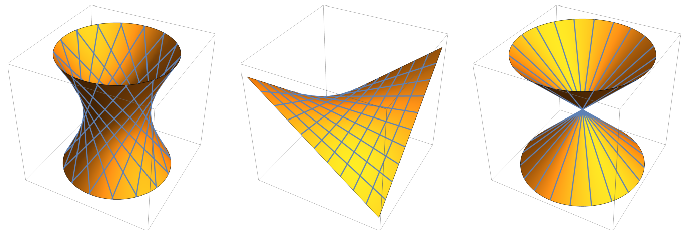
\includegraphics[width=\linewidth]{figures/quadric-surfaces-with-rulings.pdf}

我们在每个曲面上画了一些直线, 以便看出无穷多条直线是怎样分布的. 前两个曲面是光滑的, 第三个则是奇异的, 这一点在曲面上直线的分布中有所反映. 更具体地说, Exercise~\ref{ex:smooth-quadric-iff-doubly-ruled} 论证 $\mathbb{P}^{3}$ 中的二次曲面光滑当且仅当曲面的每一点恰好落在该曲面的两条直线上. 这样的曲面称为\textquotedbl{}双直纹曲面\textquotedbl{}, 前面已经见过一例: Segre 嵌入 $\mathbb{P}^{1}\times\mathbb{P}^{1}\subseteq\mathbb{P}^{3}$, 即上图中的第二个曲面. 实际上, 这本质上是唯一的例子: Exercise~\ref{ex:smooth-quadric-projectively-equivalent-to-segre-surface} 论证 $\mathbb{P}^{3}$ 中每个光滑二次曲面都与 Segre 曲面射影等价. 我们把这两道习题留到下一节, 因为在那里介绍的一些方法会有用.
\end{Example}

\BookPairedNoteLeft{
$K$ 代数闭这一贯穿全书的假设对于 Proposition~\ref{prop:quadric-surfaces-are-covered-by-lines} 至关重要: 将单位球面看成 $\mathbb{R}$ 上的一个二次曲面, 它并不包含任何 (实) 直线.
}{
注意, 若 $d\ge3$, \eqref{eq:degree-two-restriction-to-affine-line-through-point} 的右边还会出现更多系数. 要使 $X$ 包含一条经过 $a\in X$ 的直线, 这些系数也必须为零. 但三个或更多齐次多项式在 $\mathbb{P}^{2}$ 中一般没有公共解.
}
这反映出, 次数 $d\ge3$ 的曲面通常并不是每一点都有曲面中的直线通过. 因此, Proposition~\ref{prop:quadric-surfaces-are-covered-by-lines} 的证明所用的方法在 $d\ge3$ 时失效, 我们需要更精细的技巧.

为了研究 $d\ge3$ 的曲面上的直线, 现在引入一个新工具: 关联簇, 它参数化所有 $d$ 次曲面上的所有直线.

\begin{Definition}{曲面上的直线的关联簇}\leavevmode\label{def:incidence-variety-of-lines-on-surfaces}
对任意 $d\ge1$, $d$ 次曲面上的直线的\emph{关联簇}是 $\mathbb{P}_{3,d}\times\mathrm{G}(2,4)$ 的子集, 定义为
\[
  \Omega_{d}=\{([f],L)\mid L\subseteq\mathcal{V}(f)\}
  \subseteq\mathbb{P}_{3,d}\times\mathrm{G}(2,4).
\]
\end{Definition}

换句话说, $\Omega_{d}$ 的一点 $([f],L)$ 对应一个非零齐次多项式 $f\in K[x_{0},x_{1},x_{2},x_{3}]_{d}$ (相差标量因子视为相同), 以及一条恰好位于消没集 $\mathcal{V}(f)\subseteq\mathbb{P}^{3}$ 上的直线 $L\subseteq\mathbb{P}^{3}$. 为了用代数几何的工具研究关联簇, 首先验证 $\Omega_{d}$ 的确是一个簇.

\begin{Proposition}{曲面上的直线构成一个射影簇}\leavevmode\label{prop:incidence-variety-of-lines-on-surfaces-is-projective}
对 $d\ge1$, $d$ 次曲面上的直线的关联簇 $\Omega_{d}$ 是 $\mathbb{P}_{3,d}\times\mathrm{G}(2,4)$ 的闭子簇. 特别地, $\Omega_{d}$ 是射影簇.
\end{Proposition}
\begin{Proof}
考察 $[f]\in\mathbb{P}_{3,d}$ 和 $L\in\mathrm{G}(2,4)$. 为说明 $\Omega_{d}$ 在 $\mathbb{P}_{3,d}\times\mathrm{G}(2,4)$ 中闭, 我们要用 $\mathbb{P}_{3,d}$ 的坐标 (对应于多项式 $f$ 的系数) 和 $\mathrm{G}(2,4)$ 的 Plücker 坐标 (对应于包含 $\mathrm{G}(2,4)$ 的环境空间 $\mathbb{P}^{5}$ 的坐标) 的多项式约束来刻画 $([f],L)\in\Omega_{d}$ 这一条件.

对某个二维子空间 $V\subseteq K^{4}$ 写 $L=\mathbb{P}(V)$, 并令 $\{v,w\}$ 为 $V$ 的一组基. 我们请读者在 Exercise~\ref{ex:dot-product-map-onto-span} 中证明, 有一个满射 $K^{4}\to V$,
\[
  u\mapsto(u\cdot v)w-(u\cdot w)v,
\]
其中\textquotedbl{}$\cdot$\textquotedbl{}表示 $K^{4}$ 上通常的点积. 若写 $u=(a_{0},a_{1},a_{2},a_{3})$, $v=(b_{0},b_{1},b_{2},b_{3})$, $w=(c_{0},c_{1},c_{2},c_{3})$, 则 $V$ 的任一元素均可写成
\[
  (u\cdot v)w-(u\cdot w)v=(a_{0}p_{00}+\cdots+a_{3}p_{30},\ldots,
  a_{0}p_{03}+\cdots+a_{3}p_{33}),
\]
其中 $p_{ij}=b_{i}c_{j}-b_{j}c_{i}$. 根据 Plücker 映射 $\mathcal{P}_{2,4}$ 的定义, 每个非零的 $p_{ij}$ 都是直线 $L\in\mathrm{G}(2,4)\subseteq\mathbb{P}^{5}$ 的一个 Plücker 坐标 (至多相差一个符号).

条件 $([f],L)\in\Omega_{d}$ 等价于 $f$ 在 $V$ 上消没. 利用 $V$ 中点以 Plücker 坐标 $p_{ij}$ 写出的表达式, 这又等价于对任意 $a_{0},\ldots,a_{3}\in K$ 有
\[
  f(a_{0}p_{00}+\cdots+a_{3}p_{30},\ldots,a_{0}p_{03}+\cdots+a_{3}p_{33})=0.
\]
将它展开为关于 $a_{0},\ldots,a_{3}$ 的多项式: 上述消没成立当且仅当 $a_{0},\ldots,a_{3}$ 的每个单项式的系数都为零. 这些系数是 $L$ 的 Plücker 坐标与 $f$ 的系数的多项式, 因此 $\Omega_{d}$ 在 $\mathbb{P}_{3,d}\times\mathrm{G}(2,4)$ 中闭.
\end{Proof}

我们在最简单的 $d=1$ 情形中把 $\Omega_{d}$ 显式地描述为消没集.

\begin{Example}{$\Omega_{1}$ 的定义方程}\leavevmode\label{ex:equations-defining-incidence-variety-in-degree-one}
任意一点 $[f]\in\mathbb{P}_{3,1}$ 对应线性多项式 $f=\alpha_{0}x_{0}+\cdots+\alpha_{3}x_{3}$, 允许相差标量因子. 此外, 通过 Plücker 映射 $\mathcal{P}_{2,4}$, 任意一点 $L\in\mathrm{G}(2,4)$ 都可以用坐标写为
\[
  L=[p_{01}:p_{02}:p_{03}:p_{12}:p_{13}:p_{23}]\subseteq\mathbb{P}^{5}.
\]
对 $i<j$ 置 $p_{ji}=-p_{ij}$, 并置 $p_{ii}=0$. 依照 Proposition~\ref{prop:incidence-variety-of-lines-on-surfaces-is-projective} 的证明, 可验证 $f$ 在 $L\in\mathrm{G}(2,4)$ 上消没当且仅当
\[
  \alpha_{0}p_{i0}+\alpha_{1}p_{i1}+\alpha_{2}p_{i2}+\alpha_{3}p_{i3}=0
  \qquad\text{对 }i=0,1,2,3.
\]
因此, $\Omega_{1}\subseteq\mathbb{P}_{3,1}\times\mathrm{G}(2,4)$ 是四个多项式的消没集. 这些多项式对来自 $\mathbb{P}_{3,1}=\mathbb{P}^{3}$ 的四个变量 $\alpha_{0},\ldots,\alpha_{3}$ 和来自 $\mathrm{G}(2,4)\subseteq\mathbb{P}^{5}$ 的六个变量 $p_{01},\ldots,p_{23}$ 分别是线性的.
\end{Example}

因为 $\Omega_{d}$ 是乘积 $\mathbb{P}_{3,d}\times\mathrm{G}(2,4)$ 的子簇, 它自然带有到乘积每个因子的投影映射. 接下来, 我们让这两个投影映射相互配合. 第一个投影才是我们真正想研究的: 毕竟, 第一个投影是满射当且仅当对每个 $[f]\in\mathbb{P}_{3,d}$, $\mathcal{V}(f)$ 都包含一条直线. 但下一个结果会表明, 只有理解了第二个投影映射, 才能了解 $\Omega_{d}$ 的结构, 例如它的维数; 而要得到关于第一个投影映射的有用结论, 这些信息不可或缺.

\begin{Proposition}{曲面上的直线的空间的维数}\leavevmode\label{prop:dimension-of-incidence-variety-of-lines-on-surfaces}
对任意 $d\ge1$, 关联簇 $\Omega_{d}$ 不可约, 且
\[
  \dim(\Omega_{d})=\binom{d+3}{3}+2-d=\dim(\mathbb{P}_{3,d})+3-d.
\]
\end{Proposition}
\begin{Proof}
\BookPairedNoteLeft{
这一结果中出现的 $3-d$ 暗示了三次曲面 (即 $d=3$) 之所以特殊的原因.
}{
令 $\pi_{2}:\Omega_{d}\to\mathrm{G}(2,4)$ 为到 $\mathbb{P}_{3,d}\times\mathrm{G}(2,4)$ 的第二个因子的投影的限制. 为证明定理, 我们研究映射 $\pi_{2}$ 的纤维.
}
令 $L\in\mathrm{G}(2,4)$ 为 $\mathbb{P}^{3}$ 中一条直线, 可对某些线性无关的 $\ell_{0},\ell_{1}\in K[x_{0},x_{1},x_{2},x_{3}]_{1}$ 写成 $L=\mathcal{V}(\ell_{0},\ell_{1})$. 注意 $([f],L)\in\pi_{2}^{-1}(L)$ 当且仅当 $f\in\mathcal{I}(L)=\langle\ell_{0},\ell_{1}\rangle$. 换言之, $\pi_{2}^{-1}(L)$ 与 $\mathbb{P}_{3,d}$ 中下面集合的元素所代表的点有自然双射:
\[
  \langle\ell_{0},\ell_{1}\rangle\cap K[x_{0},x_{1},x_{2},x_{3}]_{d}
  \subseteq K[x_{0},x_{1},x_{2},x_{3}]_{d}.
\]
由于 $\langle\ell_{0},\ell_{1}\rangle\cap K[x_{0},x_{1},x_{2},x_{3}]_{d}$ 是 $K[x_{0},x_{1},x_{2},x_{3}]_{d}$ 的线性子空间, $\pi_{2}^{-1}(L)$ 是 $\mathbb{P}_{3,d}$ 的线性子簇, 其维数比 $\langle\ell_{0},\ell_{1}\rangle\cap K[x_{0},x_{1},x_{2},x_{3}]_{d}$ 的向量空间维数少一. 下面计算该维数.

将 $\ell_{0},\ell_{1}$ 扩充为四维向量空间 $K[x_{0},x_{1},x_{2},x_{3}]_{1}$ 的一组基 $\{\ell_{0},\ell_{1},\ell_{2},\ell_{3}\}$. 注意, 存在保持次数的 $K$-代数同构 $K[y_{0},y_{1},y_{2},y_{3}]\to K[x_{0},x_{1},x_{2},x_{3}]$, 它将 $y_{i}$ 映为 $\ell_{i}$. 此同构限制为向量空间同构
\[
  \langle y_{0},y_{1}\rangle\cap K[y_{0},y_{1},y_{2},y_{3}]_{d}
  \cong\langle\ell_{0},\ell_{1}\rangle\cap K[x_{0},x_{1},x_{2},x_{3}]_{d},
\]
所以现在只需计算前者的维数. $\langle y_{0},y_{1}\rangle\cap K[y_{0},y_{1},y_{2},y_{3}]_{d}$ 的一组基由能被 $y_{0}$ 或 $y_{1}$ 整除的单项式给出. 因此, 减去既不能被 $y_{0}$ 整除也不能被 $y_{1}$ 整除的 $d+1$ 个 $d$ 次单项式后, 算得
\[
  \dim\bigl(\langle y_{0},y_{1}\rangle\cap K[y_{0},y_{1},y_{2},y_{3}]_{d}\bigr)
  =\binom{d+3}{3}-d-1.
\]
综上两个段落的论证, 对任意 $L\in\mathrm{G}(2,4)$, 纤维 $\pi_{2}^{-1}(L)$ 是 $\mathbb{P}_{3,d}$ 的一个线性子簇, 其维数为
\begin{equation}\label{eq:dimension-of-lines-projection-fiber}
  \dim(\pi_{2}^{-1}(L))=\binom{d+3}{3}-d-2.
\end{equation}
因此, 由于 $\mathrm{G}(2,4)$ 不可约, 且 $\pi_{2}:\Omega_{d}\to\mathrm{G}(2,4)$ 是满射, 其纤维都不可约且维数相同, Theorem~\ref{thm:projective-domain-irreducible-from-equidimensional-irreducible-fibres} 蕴含 $\Omega_{d}$ 不可约. 知道 $\Omega_{d}$ 不可约之后, 就可以应用 Theorem~\ref{thm:fiber-dimension-equality-on-open-subset}, 它保证存在一个非空开集 $U\subseteq\mathrm{G}(2,4)$, 使
\[
  \dim(\Omega_{d})=\dim(\pi_{2}^{-1}(L))+\dim(\mathrm{G}(2,4))
  \qquad\text{对每个 }L\in U.
\]
因为 $\dim(\mathrm{G}(2,4))=4$, 且 $\pi_{2}$ 的所有纤维都有 \eqref{eq:dimension-of-lines-projection-fiber} 给出的同一维数, 所以
\[
  \dim(\Omega_{d})=\binom{d+3}{3}-d+2.
\]
\end{Proof}

现在可以证明本节的主要结果了.

\begin{Theorem}{每个三次曲面都包含一条直线}\leavevmode\label{thm:cubic-surface-contains-line}
对任意 $f\in K[x_{0},x_{1},x_{2},x_{3}]_{3}$ 中的齐次三次多项式, 至少存在一条直线 $L\subseteq\mathbb{P}^{3}$, 使 $L\subseteq\mathcal{V}(f)$.
\end{Theorem}
\begin{Proof}
令 $\pi_{1}:\Omega_{3}\to\mathbb{P}_{3,3}$ 为到 $\mathbb{P}_{3,3}\times\mathrm{G}(2,4)$ 的第一个因子的投影的限制. 本定理等价于断言 $\pi_{1}$ 是满射. 为导出矛盾, 假设 $\pi_{1}$ 不是满射. 由于 $\Omega_{3}$ 为射影簇, $\pi_{1}(\Omega_{3})$ 在 $\mathbb{P}_{3,3}$ 中闭. 于是由假设可知, $\pi_{1}(\Omega_{3})$ 是不可约簇 $\mathbb{P}_{3,3}$ 的真闭子簇. 因此 (Exercise~\ref{ex:quasiprojective-dimension-monotone-and-strict-for-proper-closed-subvariety}), 有
\[
  \dim(\pi_{1}(\Omega_{3}))<\dim(\mathbb{P}_{3,3})=19.
\]
但是, 由于 $\dim(\Omega_{3})=19$ (Proposition~\ref{prop:dimension-of-incidence-variety-of-lines-on-surfaces}), 而 $\dim(\pi_{1}(\Omega_{3}))<19$, Theorem~\ref{thm:fiber-dimension-lower-bound} 蕴含 $\pi_{1}$ 的每个非空纤维的维数至少为一. 另一方面, Exercise~\ref{ex:cubic-surface-containing-exactly-three-lines} 给出一个三次多项式 $f\in K[x_{0},x_{1},x_{2},x_{3}]_{3}$ 的明确例子, 使 $\mathcal{V}(f)$ 包含有限且非零条直线. 这说明纤维 $\pi_{1}^{-1}([f])$ 的维数为零, 矛盾. 因此 $\pi_{1}$ 为满射, 如所断言.
\end{Proof}

本节至此证明了, 当 $d\le3$ 时, 对任意 $[f]\in\mathbb{P}_{3,d}$ 都存在一条直线 $L\subseteq\mathcal{V}(f)$. 最后陈述 $d>3$ 时的情形, 把证明留给读者作为练习.

\begin{Proposition}{多数高次曲面不包含直线}\leavevmode\label{prop:high-degree-surfaces-containing-lines-have-large-codimension}
对 $d>3$, 使 $\mathcal{V}(f)\subseteq\mathbb{P}^{3}$ 包含直线的点 $[f]\in\mathbb{P}_{3,d}$ 的集合是 $\mathbb{P}_{3,d}$ 的闭子簇, 其余维至少为 $d-3$.
\end{Proposition}
\begin{Proof}
Exercise~\ref{ex:codimension-of-high-degree-surfaces-containing-lines}.
\end{Proof}

\BookPairedNote{
换句话说, 对 $d>3$, $\mathbb{P}_{3,d}$ 中存在由点 $[f]$ 构成的一个非空开子集, 使对应的曲面 $\mathcal{V}(f)\subseteq\mathbb{P}^{3}$ 一条直线也不包含.
}{
直观上, 曲面越弯曲, 就越不容易包含一条直线.
}
还可以换一种说法: 若 $f\in K[x_{0},x_{1},x_{2},x_{3}]$ 是次数为 $d>3$ 的齐次多项式, 则要使 $\mathcal{V}(f)\subseteq\mathbb{P}^{3}$ 包含一条直线, 它的系数必须满足某些非平凡的多项式关系. 而且随着 $d$ 增大, 相对于 $\mathbb{P}_{3,d}$ 的维数, 使 $\mathcal{V}(f)$ 包含直线的 $[f]\in\mathbb{P}_{3,d}$ 的集合越来越小, 也就是说, 为保证 $\mathcal{V}(f)$ 包含一条直线, $f$ 的系数必须满足越来越多的关系.

\BookExerciseHeading
\begin{BookExercises}
  \item\label{ex:two-lines-through-point-on-complex-quadric} 考察二次曲面 $X=\mathcal{V}(x_{0}^{2}-x_{1}^{2}-x_{2}^{2}-x_{3}^{2})\subseteq\mathbb{P}_{\mathbb{C}}^{3}$, 它的实点是 $\mathbb{A}_{0}^{3}$ 内的单位球面. 在 $X$ 中构造经过 $a=[1:0:0:1]$ 的两条不同的直线.
  \item\label{ex:lines-on-quadric-cone-pass-through-vertex} 考察二次曲面 $X=\mathcal{V}(x_{1}^{2}+x_{2}^{2}-x_{3}^{2})\subseteq\mathbb{P}_{\mathbb{C}}^{3}$, 它的实点限制在仿射开片 $\mathbb{A}_{0}^{3}$ 上是顶点位于原点的圆锥面. 证明 $X$ 中的每条直线都经过 $[1:0:0:0]$, 并用这一事实解释为什么 $X$ 中除 $[1:0:0:0]$ 以外的每一点都包含在 $X$ 的唯一一条直线中.
  \item\label{ex:dot-product-map-onto-span} 令 $v,w\in K^{4}$. 证明把 $u$ 送到 $(u\cdot v)w-(u\cdot w)v$ 的映射 $K^{4}\to K^{4}$ 是到 $v$ 和 $w$ 的张成空间上的满射.
  \item\label{ex:equations-defining-incidence-variety-in-degree-two} 写出 $\Omega_{2}$ 作为 $\mathbb{P}_{3,2}\times\mathrm{G}(2,4)$ 的子簇的定义方程.
  \item\label{ex:fibers-of-different-dimensions-for-quadric-lines} 举出 $[f]\in\mathbb{P}_{3,2}$ 的一个例子, 使纤维 $\pi_{1}^{-1}([f])\subseteq\Omega_{2}$ 的维数为一, 并举一个例子使该纤维的维数为二.
  \item\label{ex:cubic-surface-containing-exactly-three-lines} 考察三次曲面 $X=\mathcal{V}(x_{0}^{3}-x_{1}x_{2}x_{3})\subseteq\mathbb{P}^{3}$.
  \begin{enumerate}
    \item 证明 $X\cap\mathcal{V}(x_{0})$ 是 $\mathbb{P}^{3}$ 中三条直线的并.
    \item 证明仿射限制
    \[
      X_{0}=\mathcal{V}(1-x_{1}x_{2}x_{3})\subseteq\mathbb{A}^{3}
    \]
    不包含任何 (仿射) 直线. (提示: 任意仿射直线都可参数化为 $\{a+tb\mid t\in K\}$, 其中 $a,b\in\mathbb{A}^{3}$ 且 $b\ne0$.)
    \item 由此得出 $X$ 恰好包含三条直线.
  \end{enumerate}
  \item\label{ex:codimension-of-high-degree-surfaces-containing-lines} 证明 Proposition~\ref{prop:high-degree-surfaces-containing-lines-have-large-codimension}. (提示: 所讨论的集合是 $\pi_{1}(\Omega_{d})\subseteq\mathbb{P}_{3,d}$.)
\end{BookExercises}

\section{光滑三次曲面上的直线}\label{sec:lines-on-smooth-cubic-surfaces}

我们来到本书的最后一节. 本节讨论下面这个经典结果, 它最初由 Arthur Cayley (1821--1895) 和 George Salmon (1819--1904) 于 1849 年证明, 并且建立在我们前面诸多结果的基础上.

\begin{Theorem}{光滑三次曲面上的直线}\leavevmode\label{thm:smooth-cubic-surface-has-twenty-seven-lines}
令 $X\subseteq\mathbb{P}^{3}$ 为一个光滑三次曲面. 则 $X$ 恰好包含 $27$ 条直线.
\end{Theorem}

Theorem~\ref{thm:smooth-cubic-surface-has-twenty-seven-lines} 如此优美的一个原因, 是结论具有一致性: 光滑三次曲面上的直线条数既不依赖于基 (代数闭) 域, 也不依赖于定义它的三次方程. 此外, 光滑二次曲面彼此都射影等价 (Exercise~\ref{ex:smooth-quadric-projectively-equivalent-to-segre-surface}), 光滑三次曲面的情形则不同: 可以证明, 即使计及射影等价, 光滑三次曲面仍有无穷多个彼此不同的例子. 这个无穷族中的每个曲面都有同样多的直线, 十分引人注目! 作为热身, 请读者在 Exercise~\ref{ex:twenty-seven-lines-on-the-fermat-cubic} 中找出 Fermat 三次曲面上的全部 $27$ 条直线. 这是最对称的例子.

一般很难直观地看到 $\mathbb{C}$ 上的三次曲面中的各条直线, 因为复直线通常只在一个点与曲面的实点相交. 然而, $\mathbb{C}$ 上有某些三次曲面, 其所有复直线都包含实直线. 最著名的例子是 Clebsch 三次曲面, 它以 Alfred Clebsch (1833--1872) 命名.

\begin{Example}{Clebsch 三次曲面上的直线}\leavevmode\label{ex:lines-on-clebsch-cubic}
Clebsch 三次曲面定义为
\[
  X=\mathcal{V}(w^{3}+x^{3}+y^{3}+z^{3}-(w+x+y+z)^{3})\subseteq\mathbb{P}^{3}.
\]
下图从三个不同角度画出了 $X$ 的实点的一个仿射限制, 以及 $X$ 上的 $27$ 条直线. 在此仿射限制中, 它们全都能以实直线的形式看到.

\noindent\phantomsection\label{fig:clebsch-cubic-three-views}%
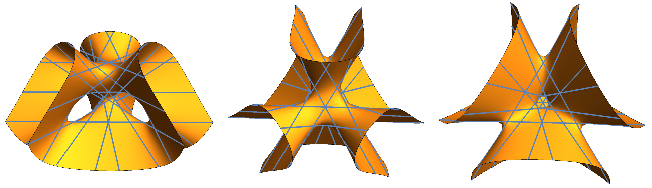
\includegraphics[width=\linewidth]{figures/clebsch-cubic-three-views.pdf}
\end{Example}

为证明 Theorem~\ref{thm:smooth-cubic-surface-has-twenty-seven-lines}, 我们先证明关于光滑三次曲面上直线的若干预备引理. 在整个过程中, 我们反复运用射影等价把直线和平面变换到便于处理的位置, 并注意这些射影等价将光滑三次曲面变为光滑三次曲面. 每一次要说明具有所需性质的射影等价存在时, 都可以把 $\mathbb{P}^{2}$ 和 $\mathbb{P}^{3}$ 中的直线和平面换成 $K^{3}$ 和 $K^{4}$ 中的线性子空间, 从而归结为线性代数的论断; 这些线性代数论证留给读者 (Exercises~\ref{ex:projective-equivalences-of-plane-line-configurations} 和~\ref{ex:projective-equivalences-of-three-space-configurations}).

下面关于光滑三次曲面上直线的引理的证明, 正是利用射影等价简化论证的典型例子.

\begin{Lemma}{在光滑三次曲面上交于一点的直线共面}\leavevmode\label{lem:concurrent-lines-on-smooth-cubic-are-coplanar}
令 $X\subseteq\mathbb{P}^{3}$ 为光滑三次曲面. 若 $X$ 上的直线 $L_{1},L_{2},L_{3}$ 满足 $L_{1}\cap L_{2}\cap L_{3}\ne\varnothing$, 则 $L_{1},L_{2},L_{3}$ 位于同一平面.
\end{Lemma}
\begin{Proof}
假设不可约三次曲面 $X\subseteq\mathbb{P}^{3}$ 包含三条交于一点但不共面的直线; 我们证明 $X$ 在这三条直线的公共交点处奇异.

给定 $\mathbb{P}^{3}$ 中三条交于一点但不共面的直线, Exercise~\ref{ex:projective-equivalences-of-three-space-configurations} 表明, 存在 $\mathbb{P}^{3}$ 的一个射影等价, 将它们送到三条直线 $\mathcal{V}(x,y)$, $\mathcal{V}(x,z)$ 和 $\mathcal{V}(y,z)$, 这三条直线交于点 $[1:0:0:0]$. 因此, 在射影等价的意义下, 可假设 $X$ 包含这三条特定直线. 令 $\mathcal{I}(X)=\langle f\rangle$. 由于 $f$ 在 $\mathcal{V}(x,y)$, $\mathcal{V}(x,z)$ 和 $\mathcal{V}(y,z)$ 上消没, 稍加思考可知, $f$ 的每一项必能被 $x,y,z$ 三个变量中至少两个整除, 因而
\[
  f=xy\ell_{1}+xz\ell_{2}+yz\ell_{3}
  \qquad\text{对某些 }\ell_{1},\ell_{2},\ell_{3}\in K[w,x,y,z]_{1}.
\]
此外, 由不可约性知 $\ell_{1},\ell_{2},\ell_{3}$ 均非零. 计算偏导数, 得
\[
  \begin{aligned}
  \frac{\partial f}{\partial w}
  &=xy\frac{\partial\ell_{1}}{\partial w}+xz\frac{\partial\ell_{2}}{\partial w}+yz\frac{\partial\ell_{3}}{\partial w},\\
  \frac{\partial f}{\partial x}
  &=y\ell_{1}+xy\frac{\partial\ell_{1}}{\partial x}+z\ell_{2}+xz\frac{\partial\ell_{2}}{\partial x}+yz\frac{\partial\ell_{3}}{\partial x},\\
  \frac{\partial f}{\partial y}
  &=x\ell_{1}+xy\frac{\partial\ell_{1}}{\partial y}+xz\frac{\partial\ell_{2}}{\partial y}+z\ell_{3}+yz\frac{\partial\ell_{3}}{\partial y},\\
  \frac{\partial f}{\partial z}
  &=xy\frac{\partial\ell_{1}}{\partial z}+x\ell_{2}+xz\frac{\partial\ell_{2}}{\partial z}+y\ell_{3}+yz\frac{\partial\ell_{3}}{\partial z}.
  \end{aligned}
\]
由于这些偏导数都在 $[1:0:0:0]\in X$ 处消没, 光滑性的 Jacobian 判据 (见 Example~\ref{ex:singularities-of-projective-hypersurfaces}) 蕴含 $X$ 在此点奇异.
\end{Proof}

下一个引理讨论光滑三次曲面与平面相交时可能出现的曲线类型. 作为准备, 回顾任意平面 $P\subseteq\mathbb{P}^{3}$ 都是某个单射的线性映射 $\mathbb{P}^{2}\to\mathbb{P}^{3}$ 的像. 由此, 只需沿这样的单射取原像, 就能将 $P$ 的任一闭子簇视为 $\mathbb{P}^{2}$ 中的射影簇. 此外, 映到同一平面 $P\subseteq\mathbb{P}^{3}$ 的任意两个单射的线性映射 $\mathbb{P}^{2}\to\mathbb{P}^{3}$ 只相差一个 $\mathbb{P}^{2}$ 的射影等价. 由于 $\mathbb{P}^{2}$ 的射影等价保持不可约曲线 $C\subseteq\mathbb{P}^{2}$ 的次数, 因而可谈论平面 $P\subseteq\mathbb{P}^{3}$ 中闭不可约曲线的\textquotedbl{}次数\textquotedbl{}. 有了这一术语, 下面的结果刻画光滑三次曲面与平面相交产生的所有可能的曲线构型.

\begin{Lemma}{光滑三次曲面的线性截面}\leavevmode\label{lem:linear-slices-of-smooth-cubic-surfaces}
令 $X\subseteq\mathbb{P}^{3}$ 为光滑三次曲面, $P\subseteq\mathbb{P}^{3}$ 为平面. 则 $X\cap P$ 恰为下列情形之一:
\begin{enumerate}[label=(\roman*),ref=\roman*]
  \item $P$ 中一条三次不可约曲线,
  \item $P$ 中一条直线与一条二次不可约曲线的并, 或
  \item\label{part:linear-slice-three-distinct-lines} $P$ 中三条不同的直线的并.
\end{enumerate}
\end{Lemma}
\begin{Proof}
令 $X\subseteq\mathbb{P}^{3}$ 为光滑三次曲面, 其中 $\mathcal{I}(X)=\langle f\rangle$, 并令 $P\subseteq\mathbb{P}^{3}$ 为平面. 用射影等价变换 $X$ 和 $P$ 后, 可假定 $P=\mathcal{V}(z)$, 并将 $P$ 与坐标为 $w,x,y$ 的 $\mathbb{P}^{2}$ 等同. $f$ 在 $P$ 上的限制由 $g=f(w,x,y,0)$ 给出, 它是 $K[w,x,y]$ 中的三次齐次多项式. 注意 $g$ 必不为零, 否则 $f$ 就能被 $z$ 整除, 与 $X$ 的不可约性矛盾.

若 $g$ 不可约, 则 $X\cap P$ 是 $P$ 中的一条三次不可约曲线. 若 $g$ 分解为一个线性多项式与一个不可约二次多项式的乘积, 则 $X\cap P$ 为 $P$ 中一条直线与一条二次不可约曲线的并. 为完成证明, 假设 $g$ 分解为三个线性多项式的乘积; 我们必须证明 $X\cap P$ 恰为三条不同的直线的并 (而不是一条或两条直线).

为导出矛盾, 假设 $X\cap P$ 包含的直线少于三条; 我们证明 $X$ 奇异. 由于 $g$ 分解为三个线性多项式的乘积, 但 $\mathcal{V}(g)=X\cap P$ 包含的直线少于三条, $g$ 必有一个重线性因子. 在射影等价的意义下, 可设这个重线性因子消没于直线 $L=\mathcal{V}(y,z)$. 换言之, 对某个非零 $\ell\in K[w,x,y,z]_{1}$, 有 $g=f(w,x,y,0)=y^{2}\ell$, 从而
\[
  f=y^{2}\ell+zq\qquad\text{对某个非零 }q\in K[w,x,y,z]_{2}.
\]
然后计算偏导数即可验证 (Exercise~\ref{ex:repeated-line-in-plane-section-produces-singularity}), 若 $q(a,b,0,0)=0$, 则 $X$ 在点 $[a:b:0:0]\in L$ 处奇异. 由于 $K$ 代数闭, 至少存在一个这样的点. 因此, 若 $X\cap P$ 为不足三条直线的并, 则 $X$ 奇异, 证明完成.
\end{Proof}

\BookPairedNoteLeft{
在 Lemma~\ref{lem:linear-slices-of-smooth-cubic-surfaces} 的情形 (\ref{part:linear-slice-three-distinct-lines}) 中, 三条直线有两种可能的分布: 要么两两相交于 $P$ 中的三个不同点, 要么三条直线相交于 $P$ 中的一个公共点.
}{
给定光滑三次曲面 $X$ 和直线 $L\subseteq X$, 接下来的目标是确定 $X$ 中与 $L$ 相交的所有其他直线. 为此, 研究 $X$ 与所有包含 $L$ 的平面的交. 更确切地说, 若 $P$ 是包含 $L$ 的平面,
}
则由 Lemma~\ref{lem:linear-slices-of-smooth-cubic-surfaces}, $X\cap P$ 或是 $L$ 与一条不可约二次曲线的并, 或还包含 $X$ 上的另外两条直线 (除 $L$ 外). 因为 $X$ 上每条与 $L$ 相交的直线恰好落在后一种平面之一中, 要了解 $X$ 上与 $L$ 相交的直线, 就要刻画哪些包含 $L$ 的平面使 $X\cap P$ 中余下的二次曲线可约. 下一个引理提供了判定一条二次曲线何时可约的计算工具.

\begin{Lemma}{判定二次曲线何时可约}\leavevmode\label{lem:reducibility-criterion-for-conics}
若 $g=ax^{2}+by^{2}+cz^{2}+dxy+exz+fyz\in K[x,y,z]$, 则 $g$ 可约当且仅当
\[
  4abc+def-af^{2}-be^{2}-cd^{2}=0.
\]
\end{Lemma}
\begin{Proof}
设 $K$ 的特征不是 $2$ (特征 $2$ 的情形留给 Exercise~\ref{ex:reducibility-criterion-for-conics-in-characteristic-two}). 给定如引理中的 $g$, 定义矩阵
\[
  M_{g}=\begin{pmatrix}
    2a&d&e\\
    d&2b&f\\
    e&f&2c
  \end{pmatrix}.
\]
注意 $2g$ 可写成矩阵乘积
\[
  2g=(x,y,z)M_{g}(x,y,z)^{T}.
\]
由
\[
  \det(M_{g})=2(4abc+def-af^{2}-be^{2}-cd^{2}),
\]
可见引理中的断言等价于: $g$ 可约当且仅当 $\det(M_{g})=0$.

令 $A=(a_{i,j})$ 为可逆 $3\times3$ 矩阵, 考察多项式 $\tilde g(x,y,z)=g((x,y,z)A^{T})$. 换言之, $\tilde g$ 由 $g$ 经 $A$ 确定的线性变量代换得到:
\[
  \tilde g(x,y,z)=g(a_{1,1}x+a_{1,2}y+a_{1,3}z,\ldots,
  a_{3,1}x+a_{3,2}y+a_{3,3}z).
\]
注意
\[
  2\tilde g=(x,y,z)A^{T}M_{g}A(x,y,z)^{T},
\]
从而有 $M_{\tilde g}=A^{T}M_{g}A$. 由于 $\det(A)=\det(A^{T})\ne0$, 由行列式的乘法性知, $\det(M_{g})=0$ 当且仅当 $\det(M_{\tilde g})=0$. 因此, $\det(M_{g})$ 是否为零, 和 $g$ 的不可约性一样, 在任意可逆线性变量代换下保持不变.

如 Proposition~\ref{prop:irreducible-conics-projectively-equivalent} 的证明所示, 在相差可逆线性变量代换的意义下, 可假设 $g=axy+bxz+cyz$. 只要注意此时 $g$ 可约当且仅当 $a,b,c$ 中有一个为零, 而这又等价于 $\det(M_{g})=2abc=0$, 就得到引理.
\end{Proof}

前两个引理汇成以下结果, 它是计数光滑三次曲面上直线的关键工具.

\begin{Lemma}{光滑三次曲面上的每条直线恰与另外 $10$ 条直线相交}\leavevmode\label{lem:line-on-smooth-cubic-meets-ten-others}
令 $X\subseteq\mathbb{P}^{3}$ 为光滑三次曲面, $L\subseteq X$ 为直线. 则恰好有五个平面 $P$ 包含 $L$, 使 $P\cap L$ 为三条直线的并. 因此, $L$ 与 $X$ 中的另外十条直线相交.
\end{Lemma}
\begin{Proof}
在射影等价的意义下, 可设 $L=\mathcal{V}(y,z)$. 设 $\mathcal{I}(X)=\langle f\rangle$. 由于 $f$ 在 $L$ 上消没, $f$ 的每一项都能被 $y$ 或 $z$ 整除. 按各项关于 $y,z$ 的次数分组, 可写
\begin{equation}\label{eq:cubic-through-line-expanded-in-transverse-variables}
  f=\ell_{1}w^{2}+\ell_{2}wx+\ell_{3}x^{2}+q_{1}w+q_{2}x+c,
\end{equation}
其中 $\ell_{1},\ell_{2},\ell_{3}\in K[y,z]_{1}$ 为线性的, $q_{1},q_{2}\in K[y,z]_{2}$ 为二次的, $c\in K[y,z]_{3}$ 为三次的.

对任意 $a=(a_{0},a_{1})\in K^{2}\setminus\{0\}$, 定义平面 $P_{a}\subseteq\mathbb{P}^{3}$ 为
\[
  P_{a}=\{[\alpha:\beta:a_{0}\gamma:a_{1}\gamma]\mid
  [\alpha:\beta:\gamma]\in\mathbb{P}^{2}\}\subseteq\mathbb{P}^{3}.
\]
注意 $P_{a}$ 包含 $L$ (即 $\gamma=0$ 的部分), 并且 $\mathbb{P}^{3}$ 中包含 $L$ 的每个平面都等于某个 $P_{a}$. 另外, $P_{a}=P_{b}$ 当且仅当对某个 $\lambda\in K\setminus\{0\}$ 有 $a=\lambda b$. 换言之, $\mathbb{P}^{3}$ 中包含 $L$ 的平面与 $\mathbb{P}^{1}$ 中的点一一对应.

用 $t,u,v$ 表示 $P_{a}$ 的定义中 $\mathbb{P}^{2}$ 上的坐标. 在这些坐标下, $f$ 在 $P_{a}$ 上的限制就是 $f^{a}=f(t,u,a_{0}v,a_{1}v)\in K[t,u,v]$, 由 \eqref{eq:cubic-through-line-expanded-in-transverse-variables}, 它等于
\[
  f^{a}=\bigl(\ell_{1}(a)t^{2}+\ell_{2}(a)tu+\ell_{3}(a)u^{2}
  +q_{1}(a)tv+q_{2}(a)uv+c(a)v^{2}\bigr)v.
\]
Lemma~\ref{lem:linear-slices-of-smooth-cubic-surfaces} 蕴含 $X\cap P_{a}$ 为三条直线的并当且仅当 $f^{a}\in K[t,u,v]$ 中的二次因子可约. 由 Lemma~\ref{lem:reducibility-criterion-for-conics}, 这当且仅当
\begin{equation}\label{eq:quintic-of-split-planes-through-cubic-line}
  4\ell_{1}\ell_{3}c+\ell_{2}q_{1}q_{2}-\ell_{1}q_{2}^{2}
  -\ell_{3}q_{1}^{2}-c\ell_{2}^{2}\in K[y,z]
\end{equation}
在 $a$ 处消没. 因此, 为证明引理, 我们必须证明 \eqref{eq:quintic-of-split-planes-through-cubic-line} 在 $\mathbb{P}^{1}$ 中恰有五个零点. 注意 \eqref{eq:quintic-of-split-planes-through-cubic-line} 是 $K[y,z]$ 中的五次齐次多项式, 所以它分解为五个线性多项式, 而我们必须证明这些线性因子互不相同.

设 $a\in\mathbb{P}^{1}$ 是 \eqref{eq:quintic-of-split-planes-through-cubic-line} 的零点, 换言之, $P_{a}\cap X$ 为三条不同直线的并. 在 $\mathbb{P}^{3}$ 的射影等价的意义下, 可假设 $P_{a}=\mathcal{V}(z)$, 等价地, $z$ 是 \eqref{eq:quintic-of-split-planes-through-cubic-line} 的线性因子. 要证明它不是重因子, 必须证明 \eqref{eq:quintic-of-split-planes-through-cubic-line} 不能被 $z^{2}$ 整除. 令 $L_{1},L_{2}$ 为 $X\cap P_{a}$ 中除 $L$ 外的两条直线. 按照 $X\cap P_{a}$ 中三条直线是否有公共交点, 分两种情况.

\textbf{(情形 1: $L\cap L_{1}\cap L_{2}=\varnothing$)} 由于三条直线 $L,L_{1},L_{2}$ 同处于平面 $P_{a}=\mathcal{V}(z)$ 内且没有公共交点, Exercise~\ref{ex:projective-equivalences-of-plane-line-configurations} 蕴含可通过射影等价将这些直线变换为 $L=\mathcal{V}(y,z)$, $L_{1}=\mathcal{V}(w,z)$ 和 $L_{2}=\mathcal{V}(x,z)$. 由于 $f$ 在 $L,L_{1},L_{2}$ 上消没, $f$ 的每一项便能被 $z$ 或 $wxy$ 整除. 从 \eqref{eq:cubic-through-line-expanded-in-transverse-variables} 可知 $z$ 整除 $\ell_{1},\ell_{3},q_{1},q_{2},c$. 由于 $f$ 不可约, $z$ 不整除 $\ell_{2}$. 因此, \eqref{eq:quintic-of-split-planes-through-cubic-line} 中除了最后一项可能例外, 每一项都能被 $z^{2}$ 整除. 要证明 $z^{2}$ 不整除 \eqref{eq:quintic-of-split-planes-through-cubic-line}, 只需证明 $z^{2}$ 不整除三次项 $c$. 最后, 假如 $z^{2}$ 整除 $c$, 则 $X=\mathcal{V}(f)$ 将在 $[0:0:1:0]$ 处奇异. 读者可以用 \eqref{eq:cubic-through-line-expanded-in-transverse-variables} 计算 $f$ 的偏导数, 并利用 $z$ 整除 $q_{1}$ 和 $q_{2}$ 以及 $z^{2}$ 整除 $c$ 来验证. 因此, $X$ 的光滑性蕴含此时 $z$ 不是 \eqref{eq:quintic-of-split-planes-through-cubic-line} 的重线性因子.

\textbf{(情形 2: $L\cap L_{1}\cap L_{2}\ne\varnothing$)} 此时, Exercise~\ref{ex:projective-equivalences-of-plane-line-configurations} 蕴含在射影等价的意义下, 可设 $L=\mathcal{V}(y,z)$, $L_{1}=\mathcal{V}(x,z)$ 和 $L_{2}=\mathcal{V}(x+y,z)$. 因此, $f$ 中不被 $z$ 整除的部分必能被 $xy(x+y)$ 整除. 从 \eqref{eq:cubic-through-line-expanded-in-transverse-variables} 可知 $z$ 整除 $\ell_{1},\ell_{2},q_{1},c$, 并且 $\ell_{3}$ 中 $y$ 的系数与 $q_{2}$ 中 $y^{2}$ 的系数相同. 特别地, 由后一事实可知, $z$ 整除 $\ell_{3}$ 当且仅当 $z$ 整除 $q_{2}$. 由于 $f$ 不可约, $z$ 不能整除两者中的任何一个, 否则 $z$ 将整除 \eqref{eq:cubic-through-line-expanded-in-transverse-variables} 中的每一项. 由于 $z$ 不整除 $q_{2}$, $z^{2}$ 不整除 $\ell_{1}q_{2}^{2}$. 又因 \eqref{eq:quintic-of-split-planes-through-cubic-line} 中的其他各项都能被 $z^{2}$ 整除, 可知 \eqref{eq:quintic-of-split-planes-through-cubic-line} 不能被 $z^{2}$ 整除. 因此, 此时 $z$ 也不是 \eqref{eq:quintic-of-split-planes-through-cubic-line} 的重线性因子.

既然已经验证 \eqref{eq:quintic-of-split-planes-through-cubic-line} 的线性因子各不相同, 便得出它在 $\mathbb{P}^{1}$ 中恰有五个零点, 给出引理陈述中的五个特殊平面. 于是得到引理的最后一个断言: $X$ 上每一条与 $L$ 相交的直线都在唯一一个包含 $L$ 的平面中. 由于 $X$ 与这个平面的交包含两条直线, Lemma~\ref{lem:linear-slices-of-smooth-cubic-surfaces} 蕴含交中一定还有第三条直线. 因此, $X$ 上每条与 $L$ 相交的直线都必在包含 $L$ 的五个特殊平面之一中, 而这样的直线 (除 $L$ 外) 恰有十条.
\end{Proof}

终于可以数出光滑三次曲面上的直线了.

\begingroup
\renewcommand{\AJProofBegin}{%
  \par\addvspace{\topsep}\noindent
  {\sffamily\bfseries\CJKfamily{pffont}Proof of Theorem~\ref{thm:smooth-cubic-surface-has-twenty-seven-lines}}\enspace\ignorespaces
}
\begin{Proof}
令 $X\subseteq\mathbb{P}^{3}$ 为光滑三次曲面, 任选 $X$ 上一条直线 $L_{1}$; 由 Theorem~\ref{thm:cubic-surface-contains-line}, 这样的直线存在. 选择一个平面 $P\subseteq\mathbb{P}^{3}$, 使 $L_{1}\subseteq P$ 且 $X\cap P$ 为三条直线的并; 由 Lemma~\ref{lem:line-on-smooth-cubic-meets-ten-others}, 这样的平面存在. 将这个平面中的另外两条直线记作 $L_{2},L_{3}$. 现在令 $L$ 是 $X$ 上任意一条别的直线. 注意 $L$ 不能位于 $P$ 内, 因为 $X\cap P$ 中仅有 $L_{1},L_{2},L_{3}$ 三条直线. 由于 $\mathbb{P}^{3}$ 中一个平面与不在其中的直线的交是单点, $L\cap P$ 是 $X\cap P=L_{1}\cup L_{2}\cup L_{3}$ 中的一个点. 因此, $L$ 与 $L_{1}\cup L_{2}\cup L_{3}$ 交于唯一一点. Lemma~\ref{lem:concurrent-lines-on-smooth-cubic-are-coplanar} 蕴含该交点不可能是 $L_{1},L_{2},L_{3}$ 中两条或更多直线的交点, 所以 $X$ 上除 $L_{1},L_{2},L_{3}$ 之外的每条直线必须恰好与这三条直线中的一条相交. 由 Lemma~\ref{lem:line-on-smooth-cubic-meets-ten-others}, $X$ 上恰有十条直线与 $L_{1},L_{2},L_{3}$ 中的每一条相交. 又由于每条 $L_{i}$ 都与 $X\cap P$ 中另外两条直线相交, $X$ 中还有八条直线与每条 $L_{i}$ 相交. 由于 $X$ 的每条直线都恰属于上述情况之一, $X$ 包含 $3+8+8+8=27$ 条直线.
\end{Proof}
\endgroup

对任意光滑三次曲面数完直线之后, 最后讨论这些直线相交的组合结构. 引人注目的是, 正如下面将看到的, 哪些直线对相交的组合结构对于每个光滑三次曲面都是一样的. 为了直观呈现哪些直线对相交, 引入光滑三次曲面 $X\subseteq\mathbb{P}^{3}$ 的\emph{直线关联图}: 这是一个 (组合) 图, $X$ 上的每条直线对应一个顶点, 两个顶点之间有边当且仅当相应的两条直线相交. 下一个结果断言此图不依赖于所选的光滑三次曲面 $X$.

\begin{Theorem}{光滑三次曲面上的直线构型}\leavevmode\label{thm:line-incidence-graph-of-smooth-cubic-is-universal}
每个光滑三次曲面都有相同的直线关联图.
\end{Theorem}
\begin{Proof}
令 $G$ 为下图. 我们断言 $G$ 是任意光滑三次曲面的直线关联图. 为此, 设 $X\subseteq\mathbb{P}^{3}$ 是光滑三次曲面; 我们说明怎样用 $X$ 上的直线给 $G$ 的顶点加标记, 使 $G$ 中两个顶点相邻当且仅当对应的两条直线在 $X$ 中相交. 鼓励读者在阅读证明时实际给 $G$ 的各顶点标上记号. 根据所作选择, 给 $G$ 加标记的方法有多种, 这反映了该图的诸多对称性. 首先可检验 $G$ 有 $27$ 个顶点, 代表 $X$ 上的 $27$ 条直线; 每个顶点都与另外 $10$ 个顶点相邻, 这反映了 Lemma~\ref{lem:line-on-smooth-cubic-meets-ten-others} 的结论.

\par\noindent\makebox[\linewidth]{%
  \phantomsection\label{fig:cubic-line-incidence-graph}%
  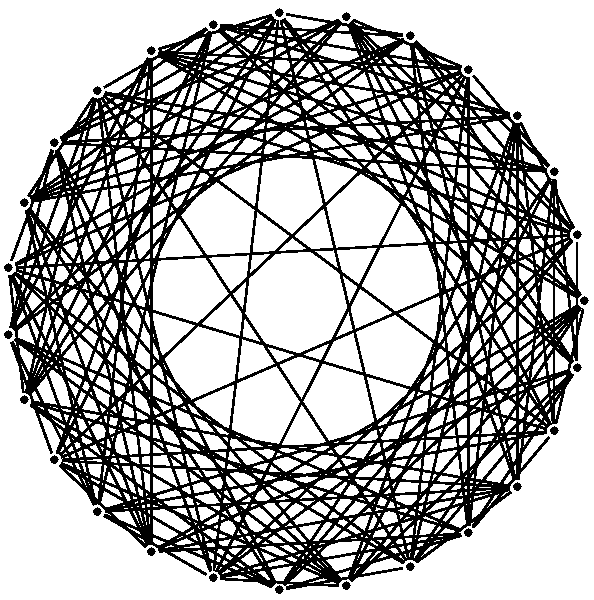
\includegraphics[width=.75\linewidth]{figures/cubic-line-incidence-graph.pdf}%
}

令 $L_{1}\subseteq X$ 为 $X$ 上任意一条直线. (\emph{任选 $G$ 的一个顶点并标记为 $L_{1}$.}) 由于 $L_{1}$ 只与 $X$ 上其余 $26$ 条直线中的十条相交, 存在一条不与 $L_{1}$ 相交的直线 $L'_{1}\subseteq X$. (\emph{任选 $G$ 中不与 $L_{1}$ 相邻的一个顶点并标记为 $L'_{1}$.}) 注意 $L_{1}$ 位于五个特殊平面中, 每个平面都包含 $X$ 上另外两条直线, 且 $L'_{1}$ 恰与每一对这样的直线中的一条相交. 用 $L_{1,2},\ldots,L_{1,6}$ 表示同时与 $L_{1}$ 和 $L'_{1}$ 相交的五条直线. (\emph{找出同时与 $L_{1}$ 和 $L'_{1}$ 相邻的五个顶点, 分别标记为 $L_{1,2},\ldots,L_{1,6}$.}) 由于 $L_{1}$ 与每条 $L_{1,i}$ 相交, 这两条相交直线所确定的平面包含 $X$ 的第三条直线, 记作 $L'_{i}$. (\emph{找出同时与 $L_{1}$ 和 $L_{1,i}$ 相邻的唯一顶点并标记为 $L'_{i}$.}) 类似地, 令 $L_{i}$ 为相交直线 $L'_{1}$ 和 $L_{1,i}$ 所确定的平面中的第三条直线. (\emph{找出同时与 $L'_{1}$ 和 $L_{1,i}$ 相邻的唯一顶点并标记为 $L_{i}$.}) 到此已找到 $X$ 上的 $17$ 条直线:
\[
  L_{1},\ldots,L_{6},L'_{1},\ldots,L'_{6},L_{1,2},\ldots,L_{1,6}.
\]
按构造, 当 $i\ge2$ 时, 形如 $\{L_{1},L_{1,i},L'_{i}\}$ 或 $\{L'_{1},L_{1,i},L_{i}\}$ 的任意三条直线共面, 所以对应顶点在直线关联图中形成三角形. 此外, 对 $1<i<j\le6$, 注意 $L_{i}$ 的选取使它与 $L_{1}$ 不相交, 而且 $L_{i}$ 也与 $L_{1,j}$ 不相交. 否则, 它必须与相交的两条直线 $L_{1,j}$ 和 $L'_{1}$ 同处一个平面, 但已知该平面中的第三条直线是 $L_{j}\ne L_{i}$. 因为 $L_{i}$ 既不与 $L_{1}$ 相交也不与 $L_{1,j}$ 相交, 所以 $L_{i}$ 必与它们所确定的平面中的第三条直线 $L'_{j}$ 相交. 类似地, 对 $1<i<j\le6$, 直线 $L'_{i}$ 与 $L_{j}$ 相交. 因此, 对所有不同的 $i,j\in\{1,\ldots,6\}$, 对应于直线对 $\{L_{i},L'_{j}\}$ 的顶点在 $X$ 的直线关联图中相邻. 本段所述直线关联图中的 $50$ 条边, 对应于 $G$ 中连接迄今已标记的 $17$ 个顶点的全部边, 读者易于验证.

对每个 $1<i<j\le6$, 注意此前找到的 $17$ 条直线中没有一条同时与两条相交的直线 $L_{i}$ 和 $L'_{j}$ 相交. 所以, $L_{i}$ 和 $L'_{j}$ 所确定的平面上的第三条直线还不在清单中, 将其记作 $L_{i,j}$. (\emph{找出同时与 $L_{i}$ 和 $L'_{j}$ 相邻的唯一顶点并标记为 $L_{i,j}$.}) 由于这样的新直线有 $10$ 条, 现在已找齐 $X$ 上的全部 $27$ 条直线. 对 $1<i<j\le6$, $L_{i,j}$ 与 $L_{1}$ 不相交, 因为与 $L_{1}$ 相交的 $10$ 条直线已全部列出. 而且 $L_{i,j}$ 与 $L_{1,i}$ 也不相交, 因为它与 $\{L'_{1},L_{1,i},L_{i}\}$ 三条直线中的另一条相交. 因此, $L_{i,j}$ 必与 $\{L_{1},L_{1,i},L'_{i}\}$ 三条直线中的 $L'_{i}$ 相交. 同理, $L_{i,j}$ 必与 $L_{j}$ 相交. 这样, 在直线关联图中, 对应于 $\{L_{i,j},L_{i}\}$, $\{L_{i,j},L'_{i}\}$, $\{L_{i,j},L_{j}\}$ 和 $\{L_{i,j},L'_{j}\}$ 各对直线的顶点都相邻, 得到直线关联图中另外 $40$ 条边.

至此已经列出了与任意 $L_{i}$ 或 $L'_{i}$ 相交的全部 $10$ 条直线, 只剩下描述哪些形如 $L_{i,j}$ 的直线彼此相交. 若 $i,j,k,\ell$ 各不相同, 由于 $L_{i,j}$ 既不与 $L_{k}$ 相交也不与 $L'_{\ell}$ 相交, 它必与 $\{L_{k},L_{k,\ell},L'_{\ell}\}$ 三条直线中的 $L_{k,\ell}$ 相交. 因此, 只要 $\{i,j\}\cap\{k,\ell\}=\varnothing$, $L_{i,j}$ 就与 $L_{k,\ell}$ 相交, 得到直线关联图中另外 $45$ 条边. 由于已描述了每个 $L_{i,j}$ 的 $10$ 个相邻顶点, 可以断定已经找齐 $X$ 的直线关联图中所有可能的边.

总之, $X$ 上的 $27$ 条直线可以分成六条彼此不相交的直线 $L_{1},\ldots,L_{6}$, 六条彼此不相交的直线 $L'_{1},\ldots,L'_{6}$, 以及 $15$ 条直线 $L_{i,j}$, 其中 $1\le i<j\le6$, 且
\begin{itemize}
  \item $L_{i}$ 与 $L'_{j}$ 相交当且仅当 $i\ne j$,
  \item $L_{i}$ 与 $L_{j,k}$ 相交当且仅当 $i\in\{j,k\}$,
  \item $L'_{i}$ 与 $L_{j,k}$ 相交当且仅当 $i\in\{j,k\}$, 并且
  \item $L_{i,j}$ 与 $L_{k,\ell}$ 相交当且仅当 $\{i,j\}\cap\{k,\ell\}=\varnothing$.
\end{itemize}
请读者核对, 这些相交关系都与按照自己标记的图 $G$ 中的 $135$ 条边一致.
\end{Proof}

\leavevmode\phantomsection\label{idx:eckardt-point}虽然 Theorem~\ref{thm:line-incidence-graph-of-smooth-cubic-is-universal} 表明每个光滑三次曲面的直线关联图都相同, 但最后指出, 直线相交的组合结构并非对所有光滑三次曲面都完全一致. 特别地, 三次曲面上的\emph{Eckardt 点}是该曲面上三条直线的公共交点. 某些特殊三次曲面有 Eckardt 点 (例如, Example~\ref{ex:lines-on-clebsch-cubic} 的图表明 Clebsch 曲面有这样的点, 而 Exercise~\ref{ex:twenty-seven-lines-on-the-fermat-cubic} 表明 Fermat 三次曲面也有), 但一般的三次曲面没有 Eckardt 点.

\BookExerciseHeading
\begin{BookExercises}
  \item\label{ex:twenty-seven-lines-on-the-fermat-cubic} 令 $X=\mathcal{V}(x_{0}^{3}+x_{1}^{3}+x_{2}^{3}+x_{3}^{3})\subseteq\mathbb{P}^{3}$ 为 Fermat 三次曲面.
  \begin{enumerate}
    \item 证明 $X$ 光滑.
    \item 给出 $X$ 上每条直线的参数化, 共 $27$ 条.
    \item 令 $\zeta$ 为一个三次单位根, 并设 $0\le i<j\le3$. 证明平面 $\mathcal{V}(x_{i}+\zeta x_{j})$ 包含 $X$ 上三条直线, 且这三条直线的交非空.
    \item 找出 $X$ 上的 $18$ 个点, 使 $X$ 上的三条直线在每个这样的点相交.
  \end{enumerate}
  \item\label{ex:projective-equivalences-of-plane-line-configurations} 证明对下列每项, 都存在满足所述性质的 $\mathbb{P}^{2}$ 的射影等价.
  \begin{enumerate}
    \item 将任意直线 $L$ 送到直线 $\mathcal{V}(x)$.
    \item 将任意一对直线 $L_{1},L_{2}$ 送到直线 $\mathcal{V}(x),\mathcal{V}(y)$.
    \item 将满足 $L_{1}\cap L_{2}\cap L_{3}=\varnothing$ 的任意三条直线 $L_{1},L_{2},L_{3}$ 送到直线 $\mathcal{V}(x),\mathcal{V}(y),\mathcal{V}(z)$.
    \item 将满足 $L_{1}\cap L_{2}\cap L_{3}\ne\varnothing$ 的任意三条直线 $L_{1},L_{2},L_{3}$ 送到直线 $\mathcal{V}(x),\mathcal{V}(y),\mathcal{V}(x+y)$.
  \end{enumerate}
  \item\label{ex:projective-equivalences-of-three-space-configurations} 证明对下列每项, 都存在满足所述性质的 $\mathbb{P}^{3}$ 的射影等价.
  \begin{enumerate}
    \item 将任意直线 $L$ 送到直线 $\mathcal{V}(y,z)$.
    \item 将任意平面 $P$ 送到平面 $\mathcal{V}(z)$.
    \item 将满足 $L_{1}\cap L_{2}\cap L_{3}\ne\varnothing$ 的任意三条不共面直线 $L_{1},L_{2},L_{3}$ 送到直线 $\mathcal{V}(x,y)$, $\mathcal{V}(x,z)$, $\mathcal{V}(y,z)$.
  \end{enumerate}
  \item\label{ex:repeated-line-in-plane-section-produces-singularity} 设 $f$ 为形如 $f=y^{2}\ell+zq$ 的不可约多项式, 其中 $\ell$ 和 $q$ 分别是 $K[w,x,y,z]_{1}$ 和 $K[w,x,y,z]_{2}$ 中的非零元素. 证明若 $q(a,b,0,0)=0$, 则 $\mathcal{V}(f)\subseteq\mathbb{P}^{3}$ 在点 $[a:b:0:0]$ 处奇异.
  \item\label{ex:reducibility-criterion-for-conics-in-characteristic-two} 设 $K$ 的特征为 $2$, 并考察齐次二次多项式 $g=ax^{2}+by^{2}+cz^{2}+dxy+exz+fyz\in K[x,y,z]$. 证明 $g$ 可约当且仅当 $def-af^{2}-be^{2}-cd^{2}=0$.
  \item\label{ex:smooth-quadric-iff-doubly-ruled} 令 $X\subseteq\mathbb{P}^{3}$ 为二次曲面.
  \begin{enumerate}
    \item 设 $X$ 光滑. 证明 $X$ 的每一点恰好包含于 $X$ 上的两条直线中.
    \item 设 $X$ 中某一点仅包含于 $X$ 上的一条直线中. 证明 $X$ 奇异.
    \item 设 $X$ 中某一点包含于 $X$ 上两条以上直线中. 证明 $X$ 奇异.
  \end{enumerate}
  \item\label{ex:smooth-quadric-projectively-equivalent-to-segre-surface} 令 $X\subseteq\mathbb{P}^{3}$ 为光滑二次曲面.
  \begin{enumerate}
    \item 证明 $X$ 包含三条彼此不相交的直线.
    \item 证明 $\mathbb{P}^{3}$ 中任意三条彼此不相交的直线与三条直线 $\mathcal{V}(w,x),\mathcal{V}(y,z),\mathcal{V}(w-y,x-z)$ 射影等价.
    \item 证明 $X$ 与 $\mathcal{V}(wz-xy)\subseteq\mathbb{P}^{3}$ 射影等价.
  \end{enumerate}
\end{BookExercises}

\chapter*{后记: 接下来往哪里走?}\label{chap:coda}
\markboth{后记}{接下来往哪里走?}
\setcounter{equation}{0}
\renewcommand{\theequation}{C.\arabic{equation}}
\renewcommand{\theHequation}{coda.\arabic{equation}}

本书已经讲了大量的数学, 但说我们不过刚刚触及代数几何的表面, 并不夸张. 这本书是一道门. 如果读者一路认真读了下来, 就已走进代数几何这座房子, 准备好去探索其中形形色色的房间. 不过, 先选择哪个房间探索, 在某种意义上取决于个人兴趣和机缘. 在这篇后记中, 我们介绍几个彼此补充的方向, 供读者读完本书后继续学习. 前两个方向聚焦于两类性质特别好, 研究得特别透彻的簇, 即代数曲线和环面簇; 第三个方向则是彻底推广簇的概念, 进入概形论的广阔天地. 希望这篇后记能让读者初步体会前方还有什么, 并为进一步掌握代数几何这门浩瀚而优美的学科指明一些方向.

\section*{代数曲线}

学习射影代数几何的许多工具, 或许最好先深入研究一维射影簇, 也就是代数曲线. 更具体些, 可以先研究射影平面曲线, 即由 $\mathbb{P}^{2}$ 中单个多项式的消没定义的射影簇. 这个范围看似很窄, 却已是一个丰富而迷人的世界, 其中包括对交理论工具的极好介绍.

关于射影平面曲线的交理论断言, 最典型的例子是本书曾简要提到的 Bézout 定理. 粗略地说, Bézout 定理断言: 若 $C_{1}=\mathcal{V}(f_{1})$ 和 $C_{2}=\mathcal{V}(f_{2})$ 是没有公共不可约分支的射影平面曲线, 且 $\deg(f_{i})=d_{i}$, 则 $C_{1}$ 与 $C_{2}$ 交于 $d_{1}\cdot d_{2}$ 个点. 然而, 涉及相切时, 必须对这句话加以限定. 例如, 曲线 $C_{1}=\mathcal{V}(y)$ 和 $C_{2}=\mathcal{V}(yz-x^{2})$ 分别由一次和二次多项式定义, 所以 Bézout 定理似乎应当告诉我们它们有两个交点, 而事实上它们的交只有一个点 $[0:0:1]$. 解决办法是注意到 $C_{1}$ 与 $C_{2}$ 在 $[0:0:1]$ 处相切, 并把这个点看成\textquotedbl{}重数\textquotedbl{}为二的交点. 一般而言, 只有按适当的重数来计数交点, Bézout 定理才成立. 精确定义交重数, 并证明它满足 Bézout 定理这样的性质, 正是交理论的起点. 对于希望在代数曲线情形下学习交重数和 Bezout 定理的学生, Fulton 的书~[\ref{bib:fulton}] 是一本经典参考书.

除了可以借此入门交理论, 曲线还有另一处值得关注: 当基域是 $\mathbb{C}$ 时, 可以借助复分析研究代数几何. 关键在于, $\mathbb{C}$ 上的光滑一维射影簇可以视为一维紧致复流形, 也称为 Riemann 曲面. 任意维的光滑射影簇也有类似性质, 但在一维时, 奇妙的是逆命题也成立: 每个紧致 Riemann 曲面作为复流形都同构于一个光滑一维射影簇. 因此, 既可以用代数几何的方法研究曲线 (把它们看成射影簇), 也可以用复分析的方法研究曲线 (把它们看成 Riemann 曲面). 代数观点和分析观点之间有着优美的相互作用. 如果读者觉得以分析的眼光看待曲线颇有启发, 可以学习 Cavalieri 和 Miles 的书~[\ref{bib:cavalieri-miles}] 或 Miranda 的书~[\ref{bib:miranda}].

除了几何以外, 代数曲线还与数论有丰富而重要的联系. 为略见一斑, 回顾鼎鼎有名的\textquotedbl{}Fermat 最后定理\textquotedbl{}: 对任意 $n\ge3$, 不存在使 $x^{n}+y^{n}=z^{n}$ 成立的正整数 $x,y,z$. 用代数几何的话说, 这个断言就是: 当 $n\ge3$ 时, 射影平面曲线 $\mathcal{V}(x^{n}+y^{n}-z^{n})\subseteq\mathbb{P}_{\mathbb{C}}^{2}$ 上不存在坐标均为非零有理数的点. 这只是数论与代数曲线上有理点的研究密切相关的初步例证. 若想从数论观点入门曲线上有理点的理论, 读者可以学习 Silverman 和 Tate 的书~[\ref{bib:silverman-tate}].

\section*{环面簇}

另一个可供继续学习的方向是环面几何, 它是进入高于一维的代数几何的一条具体且便于动手实践的途径. 简单说, 环面簇是 $\mathbb{C}$ 上的代数簇 $X$, 它含有一个与\textquotedbl{}代数环面\textquotedbl{} $T\cong(\mathbb{C}^{*})^{n}$ 同构的稠密开集, 且 $T$ 通过逐分量乘法在自身上的群作用可以延拓为 $T$ 在整个 $X$ 上的作用. 例如, 射影空间 $\mathbb{P}^{n}$ 就是环面簇, 其稠密开集由齐次坐标均非零的点构成.

环面几何的核心思想是, 只要 $X$ 上存在这个稠密的 $T$ 作用, $X$ 就具有丰富的组合结构, 从而可以完全用离散几何的语言重新解释 $X$ 的几何. 例如, 射影簇 $X$ 的一项重要代数几何信息是它的次数, 它通过计数 $X$ 与一互补维数的线性空间的交点, 粗略地衡量 $X$ 有多\textquotedbl{}弯曲\textquotedbl{}. 当 $X$ 是环面簇时, 它的次数等于相应多胞体 $P_{X}$ 的体积. 这样, 环面几何把代数几何中的一个量 (次数) 转化成了离散几何中的一个量 (体积).

凭借这种向离散情形的转化, 环面几何可以让学生在具体且便于演算例子的环境中, 初步体会代数几何中许多常用工具, 从除子理论和奇点消解, 到上同调和交理论. 不过, 须事先提醒, 在一般代数簇的广阔天地中, 环面簇只占很小一部分; 例如, 唯一的一维光滑射影环面簇是 $\mathbb{P}^{1}$. 有兴趣进一步学习环面几何的学生, 可以查阅 Cox, Little 和 Schenck 的详尽教材~[\ref{bib:cox-little-schenck}].

\section*{概形论}

这里最后提到的一个深造主题范围极广, 本身就是通往现代代数几何其他各部分的一道门, 那就是概形.

为引出概形的想法, 回顾仿射簇与有限生成既约 $K$-代数之间有一一对应 $X\mapsto K[X]$. 理解其逆对应的一种办法是回顾, $X$ 的点与 $K[X]$ 的极大理想一一对应, 所以至少作为集合, 可以把 $X$ 恢复为极大谱
\[
  \operatorname{maxSpec}(K[X])=\{\text{极大理想 }M\subseteq K[X]\}.
\]
事实上, 借此不仅可以把 $X$ 恢复为集合, 还可以恢复为拓扑空间: 仿射簇 $X$ 的 Zariski 闭子集正是形如 $\mathcal{V}(I)\subseteq X$ 的集合, 其中 $I\subseteq K[X]$ 是理想. 按照它与 $\operatorname{maxSpec}(K[X])$ 的一一对应逐项解释, 就在 $\operatorname{maxSpec}(K[X])$ 上得到一个 Zariski 拓扑, 其闭集恰为任意理想 $I\subseteq K[X]$ 所对应的集合 $Z_{I}=\{\text{极大理想 }M\supseteq I\}$.

这样, 我们描述了一个单射
\begin{equation}\label{eq:coda-maximal-spectrum}
  \begin{aligned}
    \{\text{有限生成既约 }K\text{-代数}\}&\to\{\text{拓扑空间}\}\\
    R&\mapsto\operatorname{maxSpec}(R)
  \end{aligned}
\end{equation}
其像恰由带 Zariski 拓扑的仿射簇组成. 然而, 左边是相当特殊的一类环. 因此, 自然要问, 能否将 \eqref{eq:coda-maximal-spectrum} 扩张为任意交换环 $R$ 与仿射簇的某种推广之间的一一对应. 前文已略微提示为何这样的推广会有用: 仿射曲线 $\mathcal{V}(y)\subseteq\mathbb{A}^{2}$ 与 $\mathcal{V}(y-x^{2})\subseteq\mathbb{A}^{2}$ (本篇后记前面所考察射影平面曲线的仿射限制) 相交于
\[
  X=\mathcal{V}(y)\cap\mathcal{V}(y-x^{2})=\mathcal{V}(y,y-x^{2}).
\]
若忘记 $\langle y,y-x^{2}\rangle$ 不是根理想, 就会误以为 $K[X]$ 是环
\[
  \frac{K[x,y]}{\langle y,y-x^{2}\rangle}\cong\frac{K[x]}{\langle x^{2}\rangle},
\]
它不是既约环. 这个环不是既约的, 特别是它由一个平方为零的元素生成, 这恰好反映了 $\mathcal{V}(y)$ 与 $\mathcal{V}(y-x^{2})$ 以\textquotedbl{}重数二\textquotedbl{}相交. 因此, 虽然 $K[x,y]/\langle y,y-x^{2}\rangle$ 不是簇 $X$ 的坐标环, 却可以尝试将它视为对 $X$ 的某种加强的坐标环, 这种加强记录了 $X$ 原本是一个切点这一事实.

那么, 或许只需把 \eqref{eq:coda-maximal-spectrum} 中有限生成既约 $K$-代数换成任意交换环. 遗憾的是, 这不可能是正确答案: 对任意交换环, 对应 $R\mapsto\operatorname{maxSpec}(R)$ 不是单射. 作为说明这一问题的例子, 请读者验证 $K[x]/\langle x\rangle$ 和 $K[x]/\langle x^{2}\rangle$ 各只有一个极大理想, 但两者并非同构的环.

解决办法是考虑比极大谱略大且性质更好的集合, 即素谱
\[
  \operatorname{Spec}(R)=\{\text{素理想 }P\subseteq R\}.
\]
完全按照给极大谱赋予 Zariski 拓扑的方式, 可以给这个集合赋予 Zariski 拓扑. 此外, $\operatorname{Spec}(R)$ 还从环 $R$ 继承了额外的结构, 称为\textquotedbl{}结构层\textquotedbl{} (下面再细述). 一个拓扑空间连同其上的一个环层称为\emph{赋环空间}. 由此得到映射
\begin{equation}\label{eq:coda-prime-spectrum}
  \begin{aligned}
    \{\text{交换环}\}&\to\{\text{赋环空间}\}\\
    R&\mapsto\operatorname{Spec}(R),
  \end{aligned}
\end{equation}
它终于是一个单射. 按定义, 仿射概形就是此映射的像中的赋环空间, 即形如 $\operatorname{Spec}(R)$ 的集合连同其 Zariski 拓扑和结构层, 其中 $R$ 为某个交换环. 概形论的出发点是, 将 \eqref{eq:coda-prime-spectrum} 的陪域限制为仿射概形后, 它就成为一个范畴等价, 极大地推广了贯穿本书的代数与几何的等价.

到目前为止, 对概形的讨论完全在仿射情形下进行, 于是自然会问: 是否有一个概念, 它与 (拟) 射影簇的关系, 如同仿射概形与仿射簇的关系? 这需要细致得多的处理, 因为仿射簇 $X$ 虽然完全由其正则函数环 $K[X]$ 决定, 拟射影簇却不满足这一结论.

实际上, 正如 Section~\ref{sec:continuity-of-regular-maps} 末尾所提示的, 决定拟射影簇 $X$ 的是所有开集 $U\subseteq X$ 上的环 $K[U]$ 的数据. 当两个开集 $U,V$ 相交时, 它们通过限制映射 $K[U]\to K[U\cap V]$ 联系起来. 这些数据本质上就是所谓 $X$ 上的环层. 更精确一点说, 任意拓扑空间 $X$ 上的一个\emph{环层}为每个开集 $U\subseteq X$ 指定一个环 $R(U)$, 并在 $U'\subseteq U$ 时指定一个环同态 $R(U)\to R(U')$, 这些指定须满足某些相容性条件.

特别地, 若 $X$ 是拟射影簇 (视为带有 Zariski 拓扑的拓扑空间), 则 $X$ 上有一个称为\emph{结构层}的环层 $\mathcal{O}_{X}$, 对任意开集 $U\subseteq X$ 定义为
\[
  \mathcal{O}_{X}(U)=K[U].
\]
事实上, 拟射影簇 $X$ 由赋环空间 $(X,\mathcal{O}_{X})$ 决定, 所以在这个意义下, 拟射影簇可视为赋环空间的特例. 不过, 并非所有赋环空间都是拟射影簇. 赋环空间 $(X,\mathcal{O}_{X})$ 的一个重要特征是\textquotedbl{}局部仿射\textquotedbl{}, 意思是它有一个由开集 $U_{\alpha}\subseteq X$ 组成的开覆盖, 对每个 $U_{\alpha}$, 限制 $(U_{\alpha},\mathcal{O}_{X}|_{U_{\alpha}})$ 都同构于一个仿射簇连同其结构层. 满足此条件的赋环空间 (不一定是拟射影簇) 称为\emph{抽象代数簇}. 用层的语言重述簇的概念以后, 就可以继续把概形推广到仿射情形之外: 首先, 如上所述, 描述一种在任意交换环 $R$ 的仿射概形 $\operatorname{Spec}(R)$ 上自然构造结构层的方法; 然后, 定义概形为一个赋环空间, 它有一个由作为赋环空间同构于仿射概形的开集构成的开覆盖.

概形的语言初看可能令人畏惧, 但任何希望进一步学习代数几何的学生都必须努力掌握它. 建议读者查阅 Eisenbud 和 Harris 的书~[\ref{bib:eisenbud-harris}], Hartshorne 的经典著作~[\ref{bib:hartshorne}] 或 Vakil 的书~[\ref{bib:vakil}], 开始把这些概念收入自己的数学工具箱.

\par\medskip
{\footnotesize
\noindent © 作者 2025\par
\noindent E.\ Clader, D.\ Ross, \emph{Beginning in Algebraic Geometry}, Undergraduate Texts in Mathematics.\par
\noindent
\href{https://doi.org/10.1007/978-3-031-88819-9}{doi:10.1007/978-3-031-88819-9}.\par
}

\renewcommand{\indexname}{索引}
% Keep only the TOC entry tied to the explicit index anchor below.
\begingroup
\makeatletter
\@mainmatterfalse
\makeatother
\begin{theindex}
\phantomsection\label{chap:index}
\addcontentsline{toc}{chapter}{索引}
\item Cartesian 积, \pageref{chap:products}, \pageref{sec:products-of-affine-varieties}
\item Cayley, Arthur, \pageref{sec:lines-on-smooth-cubic-surfaces}
\item Clebsch 三次曲面, \pageref{ex:lines-on-clebsch-cubic}
\item Clebsch, Alfred, \pageref{ex:lines-on-clebsch-cubic}
\item Cramer 法则, \pageref{lem:cramers-rule-over-ring}, \pageref{sec:dimension-of-tangent-spaces}
\item De Morgan 律, \pageref{def:topological-space}
\item Eckardt 点, \pageref{idx:eckardt-point}
\item Eisenstein 判别法, \pageref{prop:eisenstein-criterion}, \pageref{eq:quadratic-subalgebra-presentation}
\item Euclid 拓扑, \pageref{ex:containment-in-affine-plane}
\subitem 实数上的 Euclid 拓扑, \pageref{ex:euclidean-topology-on-real-line}
\item Euclid 引理
\subitem 整数的 Euclid 引理, \pageref{def:prime-element}
\subitem 多项式的 Euclid 引理, \pageref{ex:division-algorithm-fails-in-zz}
\item Euler 恒等式, \pageref{ex:projective-jacobian-criterion}
\item Grassmann 簇, \pageref{sec:grassmannians-and-plucker-maps}
\subitem 作为射影簇的 Grassmann 簇, \pageref{def:grassmannian-as-projective-variety}
\item Grassmann, Hermann, \pageref{sec:grassmannians-and-plucker-maps}
\item Gröbner 基, \pageref{ex:circle-in-plane-prime-ideal}
\item Hilbert 基定理, \pageref{thm:hilbert-basis-theorem}, \pageref{ex:projective-conic-and-affine-chart}
\item Hilbert, David, \pageref{thm:hilbert-basis-theorem}
\item Hironaka, Heisuke, \pageref{ex:rational-functions-form-algebra}, \pageref{ex:blowup-of-affine-cone}
\item Jacobian 矩阵, \pageref{def:jacobian-matrix}
\item Jacobian 判据, \pageref{def:smoothness-of-quasiprojective-variety}
\subitem 仿射超曲面的 Jacobian 判据, \pageref{ex:jacobian-criterion-for-hypersurfaces}
\subitem 仿射簇的 Jacobian 判据, \pageref{prop:jacobian-criterion-for-smoothness}
\subitem 射影超曲面的 Jacobian 判据, \pageref{ex:singularities-of-projective-hypersurfaces}
\item Krull 维数, \pageref{ex:krull-dimension-of-coordinate-ring}
\item Noether 环, \pageref{chap:irreducibility-of-affine-varieties}, \pageref{ex:fields-are-noetherian}, \pageref{def:irreducible-projective-variety}
\subitem Noether 环是分解整环, \pageref{ex:noetherian-ring-as-factorization-domain}
\subitem Noether 性不被子环保留, \pageref{ex:subring-need-not-be-noetherian}
\subitem Noether 性被取商保留, \pageref{ex:quotient-of-noetherian-ring}
\subitem 升链条件, \pageref{prop:ascending-chain-condition}
\subitem Hilbert 基定理, \pageref{thm:hilbert-basis-theorem}
\item Noether 基, \pageref{def:noether-basis}
\subitem Noether 基与维数, \pageref{cor:noether-basis-counts-dimension}
\subitem Noether 基与极小多项式, \pageref{lem:minimal-polynomials-and-noether-bases}
\subitem Noether 基与超越基, \pageref{ex:empty-transcendence-basis}
\item Noether 正规化定理, \pageref{chap:nullstellensatz-proof}, \pageref{thm:noether-normalization}, \pageref{prop:dimension-monotonicity}, \pageref{eq:transcendence-degree-difference-for-fibres}
\subitem Noether 正规化定理的证明, \pageref{thm:noether-normalization}
\item Noether, Emmy, \pageref{def:noetherian-ring}
\item Plücker 多项式, \pageref{ex:plucker-polynomial-in-six-variables}
\item Plücker 映射, \pageref{prop:plucker-maps-are-injective}
\subitem Plücker 映射是单射, \pageref{prop:plucker-maps-are-injective}
\subitem Plücker 映射的像, \pageref{prop:plucker-image-defined-by-plucker-polynomials}
\item Plücker, Julius, \pageref{def:plucker-maps}
\item Salmon, George, \pageref{sec:lines-on-smooth-cubic-surfaces}
\item Schubert 演算, \pageref{ex:lines-meeting-four-fixed-projective-lines}
\item Schubert, Hermann, \pageref{ex:lines-meeting-four-fixed-projective-lines}
\item Segre 映射, \pageref{def:segre-map}
\subitem Segre 映射的像, \pageref{prop:segre-map-injective-with-determinantal-image}
\item Segre, Corrado, \pageref{sec:products-and-segre-maps}
\item Veronese 簇, \pageref{ex:veronese-coordinate-products-depend-on-sum}
\item Veronese 映射, \pageref{def:veronese-map}
\subitem Veronese 映射是嵌入, \pageref{prop:veronese-maps-are-embeddings}
\subitem Veronese 映射的像, \pageref{prop:veronese-image-defined-by-quadratics}
\item Veronese, Giuseppe, \pageref{sec:veronese-maps}
\item Whitney 嵌入定理, \pageref{ex:tangent-space-of-single-point}
\item Zariski 拓扑
\subitem 仿射空间上的 Zariski 拓扑, \pageref{def:zariski-topology}
\subitem 射影空间上的 Zariski 拓扑, \pageref{def:zariski-topology-on-projective-subset}
\subitem 射影空间子集上的 Zariski 拓扑, \pageref{def:zariski-topology-on-projective-subset}
\item Zariski 引理, \pageref{lem:zariski}, \pageref{def:transcendence-basis}
\item Zariski, Oscar, \pageref{def:zariski-topology}
\item 爆破
\subitem 仿射空间的爆破, \pageref{def:blowup-of-affine-space-at-origin}
\subitem 仿射簇的爆破, \pageref{def:blowup-of-affine-variety-at-origin}
\item 闭包 (拓扑), \pageref{def:closure-and-dense-subset}
\item 闭嵌入
\subitem 仿射簇的闭嵌入, \pageref{ex:pullback-of-inclusion}
\item 不交并, \pageref{ex:two-dimensional-projective-space}
\item 不可约多项式, \pageref{sec:irreducible-polynomials}
\subitem 不可约多项式的刻画, \pageref{prop:irreducible-polynomial-characterization}
\item 不可约仿射簇, \pageref{sec:irreducible-affine-varieties}
\subitem 作为素理想的消没集的不可约仿射簇, \pageref{ex:irreducible-variety-in-finite-union}
\subitem 用消没理想刻画不可约仿射簇, \pageref{sec:irreducible-affine-varieties}
\subitem 不可约仿射簇的乘积, \pageref{prop:product-of-irreducible-varieties-is-irreducible}
\item 不可约分解
\subitem 不可约分解与不可约分解式, \pageref{prop:hypersurface-irreducible-components}
\subitem 仿射簇的不可约分解, \pageref{ex:quadric-intersection-complex-components}
\subitem 乘积的不可约分解, \pageref{cor:irreducible-components-of-product}
\subitem 射影簇的不可约分解, \pageref{prop:projective-irreducible-decomposition}
\subitem 拟射影簇的不可约分解, \pageref{prop:quasiprojective-irreducible-decomposition}
\item 不可约分支
\subitem 不可约分支与不同的不可约因子, \pageref{ex:quadric-intersection-real-components}
\subitem 仿射簇的不可约分支, \pageref{ex:quadric-intersection-real-components}
\subitem 乘积的不可约分支, \pageref{cor:irreducible-components-of-product}
\subitem 射影簇的不可约分支, \pageref{def:irreducible-projective-variety}
\subitem 拟射影簇的不可约分支, \pageref{ex:irreducible-components-of-dense-open-subvariety}
\item 不可约拟射影簇, \pageref{ex:closures-in-affine-line}
\item 不可约射影簇, \pageref{def:irreducible-projective-variety}
\item 不同的不可约分解式, \pageref{prop:radicals-of-principal-ideals}
\subitem 与不可约分解的关系, \pageref{prop:hypersurface-irreducible-components}
\item 不同的不可约因子, \pageref{prop:radicals-of-principal-ideals}
\subitem 与不可约分支的关系, \pageref{ex:irreducible-components-of-quadric-intersection}
\item 超曲面, \pageref{ex:dimension-of-unit-sphere}
\item 超越次数, \pageref{def:transcendence-degree}
\subitem 超越次数的界, \pageref{cor:bounds-on-transcendence-degree}
\item 超越基, \pageref{chap:dimension}, \pageref{def:transcendence-basis}
\subitem 超越基的大小相同, \pageref{prop:transcendence-bases-equal-size}
\subitem 超越基的存在性, \pageref{prop:finite-transcendence-basis-existence}
\item 超越数, \pageref{ex:pi-not-algebraic}
\item 乘法映射, \pageref{def:multiplicative-map}
\item 乘积
\subitem 仿射簇的乘积, \pageref{sec:products-of-affine-varieties}
\subsubitem 乘积与维数, \pageref{prop:dimension-additive-on-products}
\subsubitem 乘积与光滑性, \pageref{prop:tangent-space-of-product}
\subsubitem 仿射簇的乘积是仿射簇, \pageref{prop:product-of-affine-varieties-is-affine}
\subsubitem 乘积保持不可约性, \pageref{ex:reducible-cross-times-line}
\subitem 射影簇的乘积, \pageref{prop:segre-map-injective-with-determinantal-image}, \pageref{def:product-of-projective-varieties}
\subitem 拟射影簇的乘积, \pageref{def:product-of-quasiprojective-varieties}
\item 稠密子集
\subitem 仿射簇的稠密子集, \pageref{ex:pullback-of-inclusion}
\item 稠密子集 (拓扑), \pageref{def:closure-and-dense-subset}
\item 除法算法, \pageref{thm:polynomial-division}
\item 代数闭包, \pageref{sec:nullstellensatz}
\item 代数闭域, \pageref{def:algebraically-closed-field}, \pageref{lem:algebraic-extension-of-algebraically-closed-field}
\subitem 代数闭域为无限域, \pageref{thm:fundamental-theorem-of-algebra}
\item 代数基本定理, \pageref{thm:fundamental-theorem-of-algebra}
\item 代数相关性与代数独立性, \pageref{def:noether-basis}
\item 代数与几何的等价, \pageref{sec:equivalence-algebra-geometry}
\item 单项式, \pageref{def:monomial}
\subitem 单项式的次数, \pageref{def:polynomial-degree}
\item 导数, \pageref{sec:linearizations-and-tangent-spaces}
\item 地球, \pageref{fig:dimension-blue-marble}
\item 第一同构定理
\subitem $K$-代数的第一同构定理, \pageref{thm:first-isomorphism-theorem-k-algebras}
\subitem 环上代数的第一同构定理, \pageref{def:r-algebra}, \pageref{def:noether-basis}
\subitem 模的第一同构定理, \pageref{def:r-algebra}
\subitem 环的第一同构定理, \pageref{thm:first-isomorphism-theorem-for-rings}
\item 对偶
\subitem 线性映射的对偶, \pageref{ex:dual-and-double-dual-of-linear-map}
\subitem 向量空间的对偶, \pageref{def:dual-vector-space}
\subitem 向量空间基的对偶, \pageref{def:dual-of-a-basis}
\item 多项式, \pageref{def:polynomial-ring}
\subitem 次数的可加性, \pageref{prop:degree-additivity}
\subitem 多项式的次数, \pageref{def:polynomial-degree}
\subitem 多项式的齐次分量, \pageref{def:homogeneous-components}
\subitem 多项式的齐次化, \pageref{def:homogenization-of-polynomial}
\subitem 多项式的不可约性, \pageref{sec:irreducible-polynomials}
\subitem 首一多项式, \pageref{ex:square-root-two-integral}
\subitem 多项式的消没, \pageref{prop:polynomial-function-isomorphism}
\subitem 多项式与函数的区别, \pageref{prop:polynomial-function-isomorphism}
\item 多项式函数, \pageref{chap:coordinate-rings}, \pageref{ex:polynomial-functions-on-parabola}
\item 多项式函数的拉回
\subitem 拉回是一一对应, \pageref{prop:pullback-bijection}
\subitem 拉回的函子性, \pageref{cor:pullback-of-isomorphism}
\item 多项式环, \pageref{def:polynomial-ring}
\subitem 多项式环是分解整环, \pageref{def:unique-factorization-domain}
\subitem 多项式环是整环, \pageref{def:polynomial-ring}
\subitem 多项式环是 Noether 环, \pageref{cor:polynomial-rings-are-noetherian}, \pageref{sec:irreducible-decompositions}
\subitem 多项式环是唯一分解整环, \pageref{sec:unique-factorization-polynomial-rings}
\subitem 多项式环作为 $K$-代数, \pageref{ex:k-algebra-evaluation-homomorphisms}
\subitem 多项式环的递归性质, \pageref{prop:polynomial-ring-recursion}, \pageref{ex:polynomial-ring-as-module}
\item 多项式映射
\subitem 仿射簇之间的多项式映射, \pageref{chap:polynomial-maps}, \pageref{def:polynomial-map-between-affine-varieties}
\subitem 射影簇之间的多项式映射, \pageref{def:polynomial-maps-between-projective-varieties}
\subsubitem 射影簇之间的多项式映射是有限对一的, \pageref{cor:projective-polynomial-maps-are-finite-to-one}
\subsubitem 射影簇之间的多项式映射是线性的, \pageref{prop:projective-polynomial-maps-linear-up-to-isomorphism}
\item 多项式映射的拉回, \pageref{ex:polynomial-map-to-nodal-cubic}, \pageref{ex:pullback-preserves-multiplications}
\subitem 拉回与复合, \pageref{prop:pullback-preserves-compositions-and-identity}
\subitem 拉回与同构, \pageref{cor:pullback-of-isomorphism}
\subitem 拉回与恒等函数, \pageref{cor:pullback-of-isomorphism}
\subitem 拉回是 $K$-代数同态, \pageref{ex:pullback-by-polynomial-substitution}
\item 多项式组合, \pageref{def:polynomial-combinations-and-generators}
\item 二次曲面, \pageref{ex:lines-on-quadric-surfaces}
\item 泛光滑性, \pageref{ex:generic-smoothness-of-irreducible-hypersurfaces}
\item 范畴, \pageref{def:pullback-homomorphism}
\subitem 范畴等价, \pageref{sec:equivalence-algebra-geometry}
\item 仿射簇, \pageref{def:affine-variety}
\subitem 由理想定义的仿射簇, \pageref{prop:affine-varieties-defined-by-ideals}
\subitem 仿射簇的有限生成性, \pageref{cor:affine-varieties-finitely-generated}
\subitem 作为拟射影簇的仿射簇, \pageref{ex:punctured-affine-plane-is-not-affine}
\subitem 仿射簇之间的包含关系, \pageref{prop:operators-reverse-inclusions}
\subitem 仿射簇的交, \pageref{eq:coordinate-axes-union}, \pageref{def:zariski-topology}
\subitem 仿射簇的不可约性, \pageref{chap:irreducibility-of-affine-varieties}, \pageref{prop:irreducible-iff-vanishing-ideal-prime}
\subitem 仿射簇的不可约分支, \pageref{chap:irreducibility-of-affine-varieties}, \pageref{ex:quadric-intersection-real-components}
\subitem 仿射簇的不可约分解, \pageref{ex:quadric-intersection-complex-components}
\subitem 仿射簇的并, \pageref{eq:coordinate-axes-union}, \pageref{def:zariski-topology}
\item 仿射簇的切空间
\subitem 切空间与乘积, \pageref{prop:tangent-space-of-product}
\subitem 用局部环描述切空间, \pageref{prop:affine-tangent-space-dual-of-local-maximal-ideal-quotient}
\item 仿射簇的维数, \pageref{chap:dimension}
\subitem 维数与包含关系, \pageref{prop:dimension-monotonicity}
\subitem 维数与 Noether 基, \pageref{ex:noether-basis-for-circle}, \pageref{cor:noether-basis-counts-dimension}
\subitem 维数的公理, \pageref{def:axioms-for-dimension}
\subitem 由定义方程给出的维数界, \pageref{cor:dimension-lower-bound-by-number-of-equations}
\subitem 维数的界, \pageref{def:dimension-of-affine-variety}
\subitem 维数论基本定理, \pageref{chap:dimension}, \pageref{def:axioms-for-dimension}, \pageref{sec:fundamental-theorem-of-dimension-theory}, \pageref{ex:curves-with-arbitrarily-large-tangent-spaces}
\subsubitem 维数论基本定理的证明, \pageref{thm:fundamental-theorem-of-dimension-theory}
\subsubitem 维数论基本定理的加强形式, \pageref{thm:strong-fundamental-theorem-of-dimension-theory}
\subitem 维数的关键思想, \pageref{def:axioms-for-dimension}
\subitem 乘积的维数, \pageref{sec:geometric-properties-of-products}
\item 仿射开片, \pageref{def:affine-patches-and-restrictions}
\item 仿射空间, \pageref{def:affine-space}
\subitem 仿射空间的维数, \pageref{ex:dimension-of-affine-space}
\subitem 仿射空间的不可约性, \pageref{ex:affine-space-is-irreducible}
\subitem 仿射空间的光滑性, \pageref{ex:affine-space-is-smooth}
\item 仿射扭三次曲线, \pageref{ex:containment-in-affine-plane}
\item 仿射限制, \pageref{sec:affine-restrictions}, \pageref{def:affine-patches-and-restrictions}
\subitem 射影闭包的仿射限制, \pageref{prop:affine-restriction-of-projective-closure}
\item 仿射线性变换, \pageref{ex:translation-is-iso}
\item 仿射零点集, \pageref{def:vanishing-set}
\item 仿射零点理想, \pageref{def:vanishing-ideal}
\subitem 仿射消没理想是根理想, \pageref{def:radical-ideal}
\subitem 乘积的消没理想, \pageref{prop:vanishing-ideal-of-product}
\item 仿射锥, \pageref{def:affine-cone-over-projective-subset}
\item 非消没集, \pageref{prop:nonvanishing-sets-in-affine-closed-sets-are-affine}
\item 分解整环, \pageref{def:unique-factorization-domain}
\item 分式域, \pageref{def:fraction-field}
\item 根理想, \pageref{def:radical-ideal}
\subitem 根理想的刻画, \pageref{cor:characterize-radical-ideals}
\item 关联簇, \pageref{def:incidence-variety-of-lines-on-surfaces}
\item 光滑点
\subitem 仿射簇的光滑点, \pageref{chap:smoothness}, \pageref{sec:smooth-and-singular-points}
\subitem 拟射影簇的光滑点, \pageref{def:smoothness-of-quasiprojective-variety}
\item 光滑性
\subitem 仿射簇的光滑性, \pageref{ex:smoothness-is-intrinsic}
\subsubitem 光滑性与乘积, \pageref{prop:tangent-space-of-product}
\subitem 射影超曲面的光滑性, \pageref{ex:singularities-of-projective-hypersurfaces}
\subitem 拟射影簇的光滑性, \pageref{def:smoothness-of-quasiprojective-variety}
\item 函数域
\subitem 作为分式域的函数域, \pageref{def:function-field}
\subitem 作为有理函数集合的函数域, \pageref{prop:affine-function-field-equals-rational-function-field}
\subitem 不可约仿射簇的函数域, \pageref{chap:dimension}
\item 函子, \pageref{ex:cusp-not-isomorphic-to-line}
\subitem 全忠实函子, \pageref{ex:invert-pullback}
\item 环的不可约元, \pageref{def:units-irreducible-elements}
\item 环的代数扩张, \pageref{def:algebraic-and-integral-extensions}
\item 环的整扩张, \pageref{def:algebraic-and-integral-extensions}
\subitem 整扩张与有限生成模, \pageref{ex:rationals-algebraic-not-integral}
\item 环扩张中的代数元, \pageref{ex:pi-not-algebraic}
\item 环扩张中的整元, \pageref{def:algebraic-and-integral-elements}
\item 环上的代数, \pageref{chap:nullstellensatz-proof}, \pageref{def:r-algebra}
\item 环中的单位, \pageref{def:units-irreducible-elements}
\item 环中的素元, \pageref{def:prime-element}
\subitem 素元是不可约元, \pageref{def:units-irreducible-elements}
\item 基域, \pageref{sec:vanishing-set-operator}
\subitem 对基域的假设, \pageref{ex:weak-nullstellensatz}
\item 极大理想, \pageref{ex:linear-ideal-maximal}
\subitem 极大理想与点, \pageref{prop:single-points-and-maximal-ideals}
\subitem 极大理想是素理想, \pageref{cor:maximal-implies-prime}
\item 极小多项式, \pageref{ex:minimal-polynomial-of-square-root-two}
\subitem 极小多项式与 Noether 基, \pageref{lem:minimal-polynomials-and-noether-bases}
\item 既约环, \pageref{chap:coordinate-rings}, \pageref{def:nilpotent-elements-and-reduced-rings}
\subitem 既约环与模根理想的商, \pageref{prop:quotient-reduced-iff-ideal-radical}
\item 交叉相乘, \pageref{ex:cross-multiplied-projective-coordinates}
\item 交换引理, \pageref{lem:transcendence-basis-exchange}
\item 局部超曲面, \pageref{def:local-hypersurface}
\item 局部函数, \pageref{ex:local-functions-from-homogeneous-quotients}
\item 局部环, \pageref{prop:local-ring-unchanged-on-open-neighborhood}
\subitem 局部环的局部性, \pageref{prop:local-ring-unchanged-on-open-neighborhood}
\subitem 仿射簇的局部环, \pageref{lem:local-rings-of-affine-varieties-as-fractions}
\item 局部维数, \pageref{ex:affine-space-is-smooth}
\item 局部性质, \pageref{def:local-property-of-topological-spaces}
\item 矩阵子式, \pageref{cor:singular-locus-is-closed}
\item 空函数, \pageref{ex:empty-polynomial-function}
\item 蓝色弹珠照片, \pageref{fig:dimension-blue-marble}
\item 理想, \pageref{def:ideal}
\subitem 理想的陪集, \pageref{ex:cosets-of-variable-ideal}
\subitem 理想的有限生成性, \pageref{def:finitely-generated-ideal}
\subitem 理想的生成集, \pageref{def:ideal-generating-set}
\subitem 理想的积, \pageref{def:sum-and-product-of-ideals}
\subitem 理想的和, \pageref{def:sum-and-product-of-ideals}
\item 理想的根, \pageref{def:radical-of-an-ideal}
\subitem 理想的根是根理想, \pageref{prop:radicals-are-radical}
\item 连续映射, \pageref{def:continuous-map-of-topological-spaces}
\item 良序原理, \pageref{ex:complex-roots-of-unity}
\item 零点定理, \pageref{chap:varieties-and-ideals}, \pageref{prop:compose-vanishing-operators}, \pageref{ex:radical-is-an-ideal}, \pageref{thm:nullstellensatz}, \pageref{ex:weak-nullstellensatz}, \pageref{fig:real-hyperbola}, \pageref{ex:affine-space-is-irreducible}, \pageref{prop:hypersurface-irreducible-components}, \pageref{eq:quadratic-subalgebra-presentation}, \pageref{chap:nullstellensatz-proof}, \pageref{ex:radical-ideal-of-hypersurface-section}, \pageref{sec:dimension-of-tangent-spaces}, \pageref{ex:homogenizing-twisted-cubic-ideal}, \pageref{ex:projective-closure-of-affine-hyperbola}, \pageref{ex:regular-functions-on-projective-space-are-constant}, \pageref{eq:local-denominators-generate-unit-modulo-affine-ideal}
\subitem 射影零点定理, \pageref{sec:projective-nullstellensatz}
\subitem 零点定理的证明, \pageref{sec:proof-of-nullstellensatz}
\subitem 零点定理的陈述, \pageref{thm:nullstellensatz}
\subitem 零点定理名称的翻译, \pageref{sec:nullstellensatz}
\item 幂零元, \pageref{def:nilpotent-elements-and-reduced-rings}
\item 模, \pageref{chap:nullstellensatz-proof}, \pageref{def:r-module}
\subitem 模的有限生成性, \pageref{def:finitely-generated-module}
\subitem 模的生成元, \pageref{sec:module-generators}
\subitem 模的同态, \pageref{def:module-homomorphism}
\subitem 模的商, \pageref{def:r-algebra}
\subitem 由集合生成的子模, \pageref{ex:generated-submodule-versus-subalgebra}
\subitem 子模, \pageref{def:submodule}
\item 内在性质, \pageref{ex:intrinsic-ring-properties}
\item 拟射影簇, \pageref{chap:quasiprojective-varieties}, \pageref{def:quasiprojective-variety}
\subitem 拟射影簇是局部仿射的, \pageref{thm:quasiprojective-varieties-have-finite-affine-open-covers}
\item 拟射影簇的维数, \pageref{def:dimension-of-quasiprojective-variety}
\subitem 维数与稠密开子集, \pageref{ex:birational-equivalence-iff-dense-open-isomorphism}
\subitem 维数与包含关系, \pageref{def:dimension-of-quasiprojective-variety}
\subitem 维数论基本定理, \pageref{thm:fundamental-dimension-theorem-for-quasiprojective-varieties}
\item 扭三次曲线, \pageref{ex:projective-twisted-cubic}, \pageref{ex:homogenizing-twisted-cubic-ideal}, \pageref{ex:twisted-cubic-isomorphic-to-projective-line}
\item 偏导数, \pageref{def:linearization-of-polynomial}
\item 齐次多项式, \pageref{def:homogeneous-polynomial}
\item 齐次方程组的维数, \pageref{prop:dimension-of-homogeneous-systems}
\item 齐次化
\subitem 多项式的齐次化, \pageref{def:homogenization-of-polynomial}
\subitem 集合的齐次化, \pageref{def:homogenization-of-set}
\item 齐次理想, \pageref{def:homogeneous-ideal}
\item 齐次坐标环, \pageref{ex:isomorphism-does-not-preserve-homogeneous-coordinate-ring}
\item 奇点消解, \pageref{ex:rational-functions-form-algebra}
\item 奇异点
\subitem 仿射簇的奇异点, \pageref{chap:smoothness}, \pageref{sec:smooth-and-singular-points}
\subsubitem 奇异点集是闭集, \pageref{cor:singular-locus-is-closed}
\subitem 拟射影簇的奇异点, \pageref{def:smoothness-of-quasiprojective-variety}
\item 切空间
\subitem 仿射簇的切空间, \pageref{chap:smoothness}, \pageref{def:tangent-vector-and-tangent-space}
\subsubitem 切空间与梯度向量, \pageref{def:gradient-vector}
\subsubitem 切空间与同构, \pageref{cor:tangent-spaces-invariant-under-isomorphism}
\subsubitem 切空间与 Jacobian 矩阵, \pageref{def:jacobian-matrix}
\subsubitem 切空间是向量空间, \pageref{cor:tangent-space-is-vector-space}
\subsubitem 切空间维数的下界, \pageref{prop:tangent-dimension-lower-bound}
\subsubitem 切空间的内在刻画, \pageref{sec:intrinsic-tangent-spaces}, \pageref{cor:tangent-spaces-invariant-under-isomorphism}
\subitem 拟射影簇的切空间, \pageref{def:tangent-space-of-quasiprojective-variety}
\item 切向量, \pageref{chap:smoothness}, \pageref{def:tangent-vector-and-tangent-space}
\item 曲面, \pageref{ex:dimension-of-unit-sphere}
\item 曲线, \pageref{ex:dimension-of-unit-sphere}
\item 弱零点定理, \pageref{ex:weak-nullstellensatz}, \pageref{prop:weak-nullstellensatz}
\item 商
\subitem 模极大理想的商, \pageref{prop:prime-maximal-quotient-characterization}
\subitem 模素理想的商, \pageref{prop:prime-maximal-quotient-characterization}
\subitem 模根理想的商, \pageref{prop:quotient-reduced-iff-ideal-radical}
\subitem 代数的商, \pageref{def:k-subalgebra}
\subitem 模的商, \pageref{def:r-algebra}, \pageref{ex:quotient-module-is-well-defined}
\subitem 环的商, \pageref{def:quotient-ring}
\item 射影闭包, \pageref{def:projective-closure}, \pageref{ex:projective-closure-of-arbitrary-subset}
\subitem 超曲面的射影闭包, \pageref{prop:projective-closure-of-hypersurface}
\subitem 通过齐次化得到射影闭包, \pageref{prop:projective-closure-by-homogenizing-vanishing-ideal}
\item 射影簇, \pageref{chap:projective-varieties}, \pageref{ex:projective-varieties-in-projective-line}
\subitem 由理想定义的射影簇, \pageref{prop:projective-varieties-defined-by-ideals}
\subitem 由二次多项式定义的射影簇, \pageref{prop:projective-varieties-defined-by-quadratics}
\subitem 射影簇的有限生成性, \pageref{ex:classify-varieties-in-projective-line}
\subitem 射影簇的不可约性, \pageref{def:irreducible-projective-variety}
\subitem 射影簇的不可约分支, \pageref{def:irreducible-projective-variety}
\subitem 射影簇的不可约分解, \pageref{prop:projective-irreducible-decomposition}
\item 射影等价, \pageref{def:projective-equivalence}
\item 射影空间, \pageref{chap:projective-varieties}
\subitem 作为商的射影空间, \pageref{sec:projective-space}
\subitem 作为仿射空间延拓的射影空间, \pageref{ex:two-dimensional-projective-space}
\subitem 作为过原点直线集合的射影空间, \pageref{cor:projective-space-as-lines-through-origin}
\subitem 无穷远点, \pageref{prop:points-at-infinity-correspond-to-lines-through-origin}
\item 射影空间的线性子簇, \pageref{def:linear-subvariety-of-projective-space}
\item 射影零点定理, \pageref{sec:projective-nullstellensatz}
\item 射影消没, \pageref{def:projective-vanishing}
\item 射影消没集, \pageref{def:projective-vanishing-operator}
\item 射影消没理想, \pageref{sec:projective-ideal-operator}
\subitem 射影消没理想是齐次理想, \pageref{def:homogeneous-ideal}
\subitem 射影消没理想是根理想, \pageref{prop:projective-vanishing-ideal-is-homogeneous-radical}
\item 升链条件, \pageref{prop:ascending-chain-condition}
\item 首一多项式, \pageref{ex:square-root-two-integral}
\item 双对偶, \pageref{thm:vector-space-canonically-isomorphic-to-double-dual}
\item 双线性映射, \pageref{def:r-bilinear-map}
\item 双有理几何, \pageref{ex:rational-functions-form-algebra}
\item 双有理性
\subitem 不可约仿射簇的双有理性, \pageref{def:function-field}
\subitem 拟射影簇的双有理性, \pageref{prop:birational-iff-rational-function-rings-isomorphic}
\item 双直纹曲面, \pageref{ex:segre-quadric-is-doubly-ruled}
\item 素理想, \pageref{sec:prime-maximal-ideals}
\subitem 素理想与不可约仿射簇, \pageref{ex:irreducible-variety-in-finite-union}
\subitem 素理想是根理想, \pageref{prop:prime-ideals-are-radical}
\item 拓扑空间, \pageref{def:topological-space}
\item 梯度向量, \pageref{def:gradient-vector}
\item 同构
\subitem 仿射簇之间的同构, \pageref{def:isomorphism-of-affine-varieties}
\subitem 射影簇之间的同构, \pageref{def:isomorphism-of-projective-varieties}
\subitem 拟射影簇之间的同构, \pageref{def:isomorphism-of-quasiprojective-varieties}
\item 同构类, \pageref{sec:equivalence-algebra-geometry}
\item 同胚 (性质), \pageref{def:homeomorphism-of-topological-spaces}
\item 同胚 (映射), \pageref{def:homeomorphism-of-topological-spaces}
\item 椭圆曲线, \pageref{cor:irreducible-conics-isomorphic-to-projective-line}
\item 外在性质, \pageref{def:intrinsic-extrinsic-property}
\item 唯一分解整环, \pageref{def:unique-factorization-domain}
\item 维数论基本定理, \pageref{thm:fundamental-theorem-of-dimension-theory}, \pageref{thm:strong-fundamental-theorem-of-dimension-theory}, \pageref{thm:fundamental-dimension-theorem-for-quasiprojective-varieties}
\item 无关理想, \pageref{def:projective-irrelevant-ideal}
\item 无平方因子, \pageref{ex:square-free-generators-need-not-give-radical}
\item 纤维, \pageref{sec:theorem-on-fiber-dimensions}
\item 纤维维数定理
\subitem 第一部分, \pageref{thm:fiber-dimension-lower-bound}
\subitem 第二部分, \pageref{thm:fiber-dimension-equality-on-open-subset}
\item 线性化, \pageref{chap:smoothness}
\subitem 作为线性近似的线性化, \pageref{def:linearization-of-polynomial}
\subitem 一点处的线性化, \pageref{def:linearization-of-polynomial}
\subitem 多项式的线性化, \pageref{def:linearization-of-polynomial}
\subitem 乘积的线性化, \pageref{prop:tangent-space-of-product}
\item 线性投影, \pageref{ex:linear-projections-of-projective-varieties}
\item 线性映射
\subitem 射影簇之间的线性映射, \pageref{ex:linear-map-from-projective-quadric}
\subsubitem 射影簇之间的线性映射是有限对一的, \pageref{ex:normal-form-and-finite-fibres-of-projective-linear-map}
\subitem 向量空间之间的线性映射, \pageref{def:submodule}
\item 线性子空间, \pageref{def:submodule}
\item 线性组合, \pageref{def:module-linear-combination}
\item 向量空间, \pageref{chap:nullstellensatz-proof}
\item 向量空间的基, \pageref{fig:dimension-standard-basis}, \pageref{def:field-generators}
\item 向量空间的维数, \pageref{fig:dimension-standard-basis}
\item 向量空间之间的线性映射
\subitem 线性映射的行列式, \pageref{lem:determinant-of-multiplication}
\item 行列式
\subitem 行列式与 Cramer 法则, \pageref{lem:cramers-rule-over-ring}
\subitem 行列式与极小多项式, \pageref{lem:minimal-polynomials-and-noether-bases}
\item 行列式簇, \pageref{ex:segre-image-of-two-projective-lines}
\item 形式线性组合, \pageref{def:formal-linear-combination}
\item 一元多项式环, \pageref{sec:single-variable-polynomials}
\subitem 一元多项式环是主理想整环, \pageref{cor:univariate-polynomial-ring-pid}
\subitem 除法算法, \pageref{thm:polynomial-division}, \pageref{ex:dimension-of-finite-union}
\subitem 因式定理, \pageref{cor:polynomial-factor-theorem}
\subitem 有限零点定理, \pageref{cor:polynomial-finite-zeros}
\item 有理簇, \pageref{ex:fermat-cubic-not-rational}
\item 有理函数
\subitem 不可约仿射簇上的有理函数, \pageref{def:function-field}
\subitem 拟射影簇上的有理函数, \pageref{def:rational-function-on-quasiprojective-variety}
\item 有理函数的定义域, \pageref{def:ring-of-rational-functions}
\item 有理函数环, \pageref{def:ring-of-rational-functions}
\item 有理函数域, \pageref{prop:affine-function-field-equals-rational-function-field}
\item 有理映射, \pageref{def:rational-map-of-quasiprojective-varieties}
\item 有理映射的定义域, \pageref{def:rational-map-of-quasiprojective-varieties}
\item 有理映射的像, \pageref{def:rational-map-of-quasiprojective-varieties}
\item 有限生成性
\subitem 有限生成代数, \pageref{def:finitely-generated-k-algebra}
\subitem 有限生成域扩张, \pageref{cor:algebraic-field-extensions-transitive}
\subitem 有限生成理想, \pageref{def:finitely-generated-ideal}
\subitem 有限生成模, \pageref{def:finitely-generated-module}
\item 余维, \pageref{ex:dimension-of-unit-sphere}
\item 域的代数扩张
\subitem 代数扩张的传递性, \pageref{cor:algebraic-field-extensions-transitive}
\subitem 代数扩张的刻画, \pageref{cor:algebraic-field-extensions-transitive}
\item 域的生成元, \pageref{def:field-generators}
\item 域的特征, \pageref{ex:weak-nullstellensatz}
\item 域上的代数, \pageref{chap:coordinate-rings}, \pageref{ex:integers-not-k-algebra}
\subitem 作为环扩张的域上的代数, \pageref{ex:integers-not-k-algebra}
\subitem 域上代数的有限生成性, \pageref{def:finitely-generated-k-algebra}
\subitem 域上代数的第一同构定理, \pageref{thm:first-isomorphism-theorem-k-algebras}
\subitem 域上代数的生成元, \pageref{sec:generators-of-k-algebras}
\subitem 域上代数的同态, \pageref{def:k-algebra-homomorphism}
\subitem 域上代数中的多项式组合, \pageref{def:polynomial-combinations-and-generators}
\subitem 域上代数的表示, \pageref{ex:generated-subalgebra-is-smallest}
\subitem 域上代数的商, \pageref{prop:quotient-k-algebra}
\subitem 域上代数的子代数, \pageref{def:k-subalgebra}
\item 占优映射
\subitem 仿射簇之间的占优映射, \pageref{ex:pullback-of-inclusion}
\item 张量积, \pageref{chap:products}, \pageref{sec:tensor-products-of-modules}
\subitem 张量积与乘积的坐标环, \pageref{ex:coordinate-ring-of-cylinder}
\subitem 标量扩张, \pageref{ex:extension-of-scalars-has-module-structure}
\subitem 代数的张量积, \pageref{prop:tensor-product-of-algebras-is-algebra}
\subsubitem 张量积与双线性, \pageref{sec:tensor-products-and-bilinearity}
\subitem 模的张量积, \pageref{def:tensor-product-of-modules}
\subsubitem 张量积与双线性, \pageref{sec:tensor-products-and-bilinearity}
\subitem 关系, \pageref{ex:rewrite-tensor-in-three-ways}
\subitem 简单张量, \pageref{prop:tensor-product-of-algebras-is-algebra}
\item 整闭包, \pageref{ex:integral-closure-is-subring}
\item 正则函数
\subitem 仿射簇上的正则函数, \pageref{thm:regular-functions-on-affine-varieties-are-polynomial}
\subitem 拟射影簇上的正则函数, \pageref{def:regular-function-on-quasiprojective-variety}
\item 正则函数环, \pageref{def:ring-of-regular-functions}
\item 正则映射
\subitem 正则映射是连续的, \pageref{thm:regular-maps-are-zariski-continuous}
\subitem 射影簇之间的正则映射, \pageref{def:regular-maps-between-projective-varieties}
\subitem 拟射影簇之间的正则映射, \pageref{def:regular-map-of-quasiprojective-varieties}
\item 正则映射的拉回, \pageref{ex:ring-invariance-under-quasiprojective-isomorphism}
\item 正则映射的图像, \pageref{def:graph-of-quasiprojective-regular-map}
\item 直和, \pageref{fig:circle-times-line-cylinder}
\item 直线关联图, \pageref{thm:line-incidence-graph-of-smooth-cubic-is-universal}
\item 指标集, \pageref{ex:intersection-and-union-via-ideals}
\item 秩-零化度定理, \pageref{ex:invertible-affine-linear-map}, \pageref{ex:prove-dimension-function-unique}, \pageref{sec:theorem-on-fiber-dimensions}
\item 主理想, \pageref{ex:variables-ideal-not-principal}
\item 主理想的根, \pageref{prop:radicals-of-principal-ideals}
\item 主理想整环, \pageref{def:principal-ideal-domain}
\subitem 主理想整环是唯一分解整环, \pageref{def:principal-ideal-domain}
\item 子簇, \pageref{def:subvariety-of-quasiprojective-variety}
\item 子空间拓扑, \pageref{def:subspace-topology}
\item 自由模, \pageref{def:free-module-on-a-set}
\item 坐标函数, \pageref{ex:coordinate-functions}, \pageref{ex:generated-subalgebra-is-smallest}
\item 坐标环, \pageref{chap:coordinate-rings}, \pageref{def:coordinate-ring}
\subitem 坐标环与坐标函数, \pageref{cor:coordinate-ring-finitely-generated}
\subitem 作为 $K$-代数的坐标环, \pageref{prop:coordinate-ring-as-quotient-k-algebra}
\subitem 作为多项式函数环的坐标环, \pageref{ex:coordinate-ring-of-empty-set}
\subitem 作为商的坐标环, \pageref{ex:coordinate-ring-of-parabola}, \pageref{prop:coordinate-ring-as-quotient-k-algebra}
\subitem 作为正则函数环的坐标环, \pageref{ex:regular-function-ring-of-punctured-projective-conic}
\subitem 坐标环的刻画, \pageref{prop:coordinate-rings-as-finitely-generated-reduced-algebras}
\subitem 用坐标环判别同构, \pageref{cor:coordinate-rings-detect-isomorphisms}
\subitem 乘积的坐标环, \pageref{sec:coordinate-rings-of-products}
\end{theindex}
\endgroup

\chapter*{参考文献}\label{chap:bibliography}
\markboth{参考文献}{参考文献}

\begin{enumerate}[label={[\arabic*]},ref=\arabic*,leftmargin=*,align=left]
  \item\label{bib:cavalieri-miles} Renzo Cavalieri and Eric Miles. \emph{Riemann Surfaces and Algebraic Curves: A First Course in Hurwitz Theory}. Cambridge University Press, 2016.
  \item\label{bib:cox-little-oshea} David A. Cox, John Little, and Donal O’Shea. \emph{Ideals, Varieties, and Algorithms: An Introduction to Computational Algebraic Geometry and Commutative Algebra}. Springer, 2015.
  \item\label{bib:cox-little-schenck} David A. Cox, John B. Little, and Henry K. Schenck. \emph{Toric Varieties}. American Mathematical Society, 2011.
  \item\label{bib:eisenbud-harris} David Eisenbud and Joe Harris. \emph{The Geometry of Schemes}. Springer, 2000.
  \item\label{bib:fulton} William Fulton. \emph{Algebraic Curves}. Addison-Wesley, 1989.
  \item\label{bib:hartshorne} Robin Hartshorne. \emph{Algebraic Geometry}. Springer, 1977.
  \item\label{bib:miranda} Rick Miranda. \emph{Algebraic Curves and Riemann Surfaces}. American Mathematical Society, 1995.
  \item\label{bib:shafarevich} Igor R. Shafarevich. \emph{Basic Algebraic Geometry 1: Varieties in Projective Space}. Springer, 2013.
  \item\label{bib:silverman-tate} Joseph H. Silverman and John Tate. \emph{Rational Points on Elliptic Curves}. Springer, 1992.
  \item\label{bib:smith-et-al} Karen E. Smith, Lauri Kahanpää, Pekka Kekäläinen, and William Traves. \emph{An Invitation to Algebraic Geometry}. Springer, 2000.
  \item\label{bib:vakil} Ravi Vakil. \emph{The Rising Sea: Foundations of Algebraic Geometry}, 2017.
\end{enumerate}

\par\medskip
{\footnotesize
\noindent © 作者 2025\par
\noindent E.\ Clader, D.\ Ross, \emph{Beginning in Algebraic Geometry}, Undergraduate Texts in Mathematics.\par
\noindent
\href{https://doi.org/10.1007/978-3-031-88819-9}{doi:10.1007/978-3-031-88819-9}.\par
}

\end{document}
